\documentclass[ps2pdf,11pt,report]{SANDreport}
%\documentclass[a4paper]{book}
%\usepackage{a4wide}

% Shortcuts for Dakota information incorporated in multiple versions of manuals
%
% This file is included in all top-level .tex files

% When using this command, likely follow with a forced space, e.g., one of
% Version \DakotaVersion\ Manual
% Version \DakotaVersion\space Manual
% Version \DakotaVersion{} Manual
\newcommand{\DakotaVersion}{6.4}


% Most recent SAND report numbers and report date based on
% Data should be SAND report date and not reflect updates
\newcommand{\DakotaSANDDate}{July 2014}
\newcommand{\DakotaSANDDev}{SAND2014-5014}
\newcommand{\DakotaSANDRef}{SAND2014-5015}
\newcommand{\DakotaSANDUsers}{SAND2014-4633}
\newcommand{\DakotaSANDTheory}{SAND2014-4253}


% Need to manually break line or Eldred gets incorrectly split
\newcommand{\DakotaAuthorSAND}{
Brian~M.~Adams, Lara~E.~Bauman, William~J.~Bohnhoff, Keith~R.~Dalbey,\\ 
John~P.~Eddy, Mohamed~S.~Ebeida, Michael~S.~Eldred, Russell~W.~Hooper,\\
Patricia~D.~Hough, Kenneth~T.~Hu, John~D.~Jakeman, Kathryn~A.~Maupin,\\
Jason~A.~Monschke, Ahmad~Rushdi,Laura~P.~Swiler, J.~Adam~Stephens,\\
Dena~M.~Vigil, Timothy~M.~Wildey
}

\newcommand{\authvskip}{0.25cm}

\newcommand{\DakotaAuthorLong}{
{Brian~M.~Adams, Mohamed~S.~Ebeida, Michael~S.~Eldred, John~D.~Jakeman,}\\
{Kathryn~A.~Maupin, Jason~A.~Monschke, Laura~P.~Swiler, J.~Adam~Stephens,}\\
{Dena~M.~Vigil, Timothy~M.~Wildey}\\
{\sl Optimization and Uncertainty Quantification Department} \vspace*{\authvskip} \\ 
{William~J.~Bohnhoff,} {\sl Radiation Transport Department} \vspace*{\authvskip} \\
{John~P.~Eddy,} {\sl System Readiness and Sustainment Technologies Department} \vspace*{\authvskip} \\
{Russell~W.~Hooper,} {\sl Multiphysics Applications Department} \vspace*{\authvskip} \\
{Kenneth~T.~Hu,} {\sl Validation and Uncertainty Quantification Department} \vspace*{\authvskip} \\
{Keith~R.~Dalbey,} {\sl Mission Analysis and Simulation Department} \vspace*{\authvskip} \\
{Lara~E.~Bauman, Patricia~D.~Hough} \\
{\sl Quantitative Modeling and Analysis Department} \vspace*{\authvskip} \\
Sandia National Laboratories\\
P.O. Box 5800\\
Albuquerque, NM 87185 \vspace*{\authvskip} \\
{Ahmad~Rushdi,} {\sl Institute for Computational and Engineering Sciences} \vspace*{\authvskip} \\
The University of Texas at Austin\\
P.O. Box 4.102\\
Austin, TX 78712\\
}

\newcommand{\DakotaAuthorFormatted}{
{\large \bf Brian M. Adams, Mohamed S. Ebeida, Michael S. Eldred, John D. Jakeman,\\
Kathryn~A.~Maupin, Jason~A.~Monschke, Laura P. Swiler, J. Adam Stephens, Dena M. Vigil,\\
Timothy M. Wildey}\\ 
{\large Optimization and Uncertainty Quantification Department}\\
\vspace*{\authvskip}
{\large \bf William J. Bohnhoff}\\
{\large Radiation Transport Department}\\
\vspace*{\authvskip}
{\large \bf Keith R. Dalbey}\\
{\large Mission Analysis and Simulation Department}\\
\vspace*{\authvskip}
{\large \bf John P. Eddy}\\
{\large System Readiness and Sustainment Technologies Department}\\
\vspace*{\authvskip}
{\large \bf Russell W. Hooper}\\
{\large Multiphysics Applications Department}\\
\vspace*{\authvskip}
{\large \bf Kenneth T. Hu}\\
{\large Validation and Uncertainty Quantification Department}\\
\vspace*{\authvskip}
{\large \bf Lara E. Bauman, Patricia D. Hough}\\
{\large Quantitative Modeling and Analysis Department}\\
\vspace*{\authvskip}
{\large Sandia National Laboratories}\\
{\large P.O. Box 5800}\\
{\large Albuquerque, New Mexico 87185}\\
\vspace*{\authvskip}
{\large \bf Ahmad Rushdi}\\
{\large Institute for Computational and Engineering Sciences}\\
\vspace*{\authvskip}
{\large The University of Texas at Austin}\\
{\large P.O. Box 4.102}\\
{\large Austin, TX 78712}\\
}


% Fragments which together comprise abstracts

\newcommand{\DakotaAbstractShared}{
The Dakota (Design Analysis Kit for Optimization and Terascale
Applications) toolkit provides a flexible and extensible interface
between simulation codes and iterative analysis methods. Dakota 
contains algorithms for optimization with gradient and
nongradient-based methods; uncertainty quantification with sampling,
reliability, and stochastic expansion methods; parameter
estimation with nonlinear least squares methods; and
sensitivity/variance analysis with design of experiments and parameter
study methods. These capabilities may be used on their own or as
components within advanced strategies such as surrogate-based
optimization, mixed integer nonlinear programming, or optimization
under uncertainty. By employing object-oriented design to implement
abstractions of the key components required for iterative systems
analyses, the Dakota toolkit provides a flexible and extensible
problem-solving environment for design and performance analysis of
computational models on high performance computers.
% blank line intended

% blank line intended
}

\newcommand{\DakotaAbstractDev}{
This report describes the Dakota class hierarchies. It is derived 
from annotation of the source code and provides detailed class 
documentation, including all member functions and attributes.  
}

\newcommand{\DakotaAbstractRef}{
This report serves as a reference manual for the commands specification
for the Dakota software, providing input overviews, option descriptions,
and example specifications.
}

\newcommand{\DakotaAbstractUsers}{
This report serves as a user's manual for the Dakota software and
provides capability overviews and procedures for software execution,
as well as a variety of example studies.
}

\newcommand{\DakotaAbstractTheory}{
This report serves as a theoretical manual for selected algorithms
implemented within the Dakota software.  It is not intended as a
comprehensive theoretical treatment, since a number of existing texts
cover general optimization theory, statistical analysis, and other
introductory topics.  Rather, this manual is intended to summarize a
set of Dakota-related research publications in the areas of
surrogate-based optimization, uncertainty quantification, and
optimization under uncertainty that provide the foundation for many 
of Dakota's iterative analysis capabilities.
}

\usepackage{makeidx}
\usepackage{fancyhdr}
\usepackage{graphicx}
\usepackage{wrapfig}
\usepackage{bigbox}
\usepackage{subfigure}
\usepackage{moreverb}
\usepackage{float}
\usepackage{alltt}
\usepackage{times}
\ifx\pdfoutput\undefined
\usepackage[ps2pdf,
            pagebackref=true,
            colorlinks=true,
            linkcolor=blue
           ]{hyperref}
\else
\usepackage[pdftex,
            pagebackref=true,
            colorlinks=true,
            linkcolor=blue
           ]{hyperref}
\fi
\usepackage{colortbl}

%\usepackage{doxygen}
% Some settings borrowed from doxygen.sty:
\pagestyle{fancyplain}
\setlength{\parindent}{0cm}
\setlength{\parskip}{0.2cm}
\lhead[\fancyplain{}{\bfseries\thepage}]
        {\fancyplain{}{\bfseries\rightmark}}
\rhead[\fancyplain{}{\bfseries\leftmark}]
        {\fancyplain{}{\bfseries\thepage}}
\rfoot[\fancyplain{}{\bfseries\scriptsize DAKOTA Version \DakotaVersion\space User's Manual generated on \today}]{}
\lfoot[]{\fancyplain{}{\bfseries\scriptsize DAKOTA Version \DakotaVersion\space User's Manual generated on \today}}
\cfoot{}

\title{DAKOTA, A Multilevel Parallel Object-Oriented Framework for 
Design Optimization, Parameter Estimation, Uncertainty Quantification, 
and Sensitivity Analysis\\\vspace{5mm}Version \DakotaVersion\space User's Manual}

\author{\DakotaAuthorLong}

\date{\today}

\SANDnum{\DakotaSANDUsers}
\SANDprintDate{\today}
\SANDauthor{\DakotaAuthorSAND}
\SANDreleaseType{Unlimited Release}

\makeindex
\setcounter{tocdepth}{1}
\renewcommand\footrulewidth{0.4pt}

\begin{document}

\maketitle

\begin{abstract}
\DakotaAbstractShared
\DakotaAbstractUsers
\end{abstract}

\pagenumbering{arabic}
%\setcounter{page}{3}

% \newcommand{\clearemptydoublepage} defined in doxygen.sty as:
\newpage{\pagestyle{empty}\cleardoublepage}

\tableofcontents
%\listoffigures
%\listoftables

% \newcommand{\clearemptydoublepage} defined in doxygen.sty as:
\newpage{\pagestyle{empty}\cleardoublepage}

\SANDmain 

%\setcounter{secnumdepth}{-1} % Turn off chapter numbering (for the Preface)
%\chapter{DAKOTA Users Manual}
%\label{index}\hypertarget{index}{}\input{index}
\chapter*{Preface}
\addcontentsline{toc}{chapter}{Preface}
%\chapter{Preface}

The Dakota (Design Analysis Kit for Optimization and Terascale
Applications) project started in 1994 as an internal research and
development activity at Sandia National Laboratories in Albuquerque,
New Mexico. The original goal was to provide a common set of
optimization tools for a group of engineers solving structural
analysis and design problems. Prior to the Dakota project, there was
no focused effort to archive optimization methods for reuse on other
projects. Thus, engineers found themselves repeatedly building new
custom interfaces between the engineering analysis software and
optimization software. This was especially burdensome when using
parallel computing, as each project developed a unique master program
to coordinate concurrent simulations on a network of workstations or a
parallel computer. The initial Dakota toolkit provided the engineering
and analysis community at Sandia access to a variety of optimization
algorithms, hiding the complexity of the optimization software
interfaces from the users. Engineers could readily switch between
optimization software packages by simply changing a few lines in a
Dakota input file. In addition to structural analysis, Dakota has been
applied to computational fluid dynamics, nonlinear dynamics, shock
physics, heat transfer, electrical circuits, and many other science
and engineering models.

Dakota has grown significantly beyond an optimization toolkit.  In
addition to its state-of-the-art optimization methods, Dakota includes
methods for global sensitivity and variance analysis, parameter
estimation, uncertainty quantification, and verification, as well as
meta-level strategies for surrogate-based optimization, hybrid
optimization, and optimization under uncertainty. Available to all
these algorithms is parallel computation support; ranging from desktop
multiprocessor computers to massively parallel computers typically
found at national laboratories and supercomputer centers.

As of Version 5.0, Dakota is publicly released as open source under a
GNU Lesser General Public License and is available for free download
world-wide.  See \url{http://www.gnu.org/licenses/lgpl.html} for more
information on the LGPL software use agreement.  Dakota Versions 3.0
through 4.2+ were licensed under the GNU General Public License.
Dakota public release facilitates research and software collaborations
among Dakota developers at Sandia National Laboratories and other
institutions, including academic, government, and corporate
entities. See the Dakota FAQ at
\url{http://dakota.sandia.gov/faq.html} for more information on the
public release rationale and ways to contribute.

Dakota leadership includes Brian Adams (project lead), Mike Eldred
(founder and research lead), Dena Vigil (support manager), and Jim
Stewart (business manager).  For a listing of current and former
contributors and third-party library developers, visit the Dakota
webpage at \url{http://dakota.sandia.gov}.

\textbf{Contact Information}:\\
{\small Brian M. Adams, Dakota Project Lead}\\
{\small Sandia National Laboratories}\\
{\small P.O. Box 5800, Mail Stop 1318}\\
{\small Albuquerque, NM 87185-1318}\\
{\small Web (including support information): \url{http://dakota.sandia.gov}}

%\setcounter{secnumdepth}{2} % Turn on chapter numbering (after the Preface)
\chapter{Introduction}\label{introduction}

\section{Motivation for Dakota Development}\label{introduction:motivation}

Computational models are commonly used in engineering design and
scientific discovery activities for simulating complex physical
systems in disciplines such as fluid mechanics, structural dynamics,
heat transfer, nonlinear structural mechanics, shock physics, and many
others. These simulators can be an enormous aid to engineers who want
to develop an understanding and/or predictive capability for complex
behaviors typically observed in the corresponding physical
systems. Simulators often serve as virtual prototypes, where a set of
predefined system parameters, such as size or location dimensions and
material properties, are adjusted to improve the performance of a
system, as defined by one or more system performance objectives. Such
optimization or tuning of the virtual prototype requires executing the
simulator, evaluating performance objective(s), and adjusting the
system parameters in an iterative, automated, and directed way. System
performance objectives can be formulated, for example, to minimize
weight, cost, or defects; to limit a critical temperature, stress, or
vibration response; or to maximize performance, reliability,
throughput, agility, or design robustness.  In addition, one would
often like to design computer experiments, run parameter studies, or
perform uncertainty quantification. These approaches reveal how system
performance changes as a design or uncertain input variable changes.
Sampling strategies are often used in uncertainty quantification to
calculate a distribution on system performance measures, and to
understand which uncertain inputs contribute most to the variance of
the outputs.

A primary goal for Dakota (Design Analysis Kit for Optimization and
Terascale Applications) development is to provide engineers and other
disciplinary scientists with a systematic and rapid means to obtain
improved or optimal designs or understand sensitivity or uncertainty
using simulation-based models. These capabilities generally lead to
improved designs and system performance in earlier design stages,
alleviating dependence on physical prototypes and testing, shortening
design cycles, and reducing product development costs. In addition to
providing this practical environment for answering system performance
questions, the Dakota toolkit provides an extensible platform for the
research and rapid prototyping of customized methods and
strategies~\cite{Eld98b}.

\section{Capabilities of Dakota}\label{introduction:capabilities}

The Dakota toolkit provides a flexible, extensible interface between
your simulation code and a variety of iterative methods and
strategies. While Dakota was originally conceived as an easy-to-use
interface between simulation codes and optimization algorithms, recent
versions have been expanded to interface with other types of iterative
analysis methods such as uncertainty quantification with
nondeterministic propagation methods, parameter estimation with
nonlinear least squares solution methods, and sensitivity/variance
analysis with general-purpose design of experiments and parameter
study capabilities. These capabilities may be used on their own or as
building blocks within more sophisticated strategies such as hybrid
optimization, surrogate-based optimization, or optimization under
uncertainty.

Thus, one of the primary advantages that Dakota has to offer is that
access to a broad range of iterative capabilities can be obtained
through a single, relatively simple interface between Dakota and your
simulator. Should you want to try a different type of iterative method
or strategy with your simulator, it is only necessary to change a few
commands in the Dakota input and start a new analysis. The need to
learn a completely different style of command syntax and the need to
construct a new interface each time you want to use a new algorithm
are eliminated.

\section{How Does Dakota Work?}\label{introduction:how}

Figure~\ref{introduction:bbinterface} depicts a typical
loosely-coupled, or ``black-box,'' relationship between Dakota and the
simulation code(s).  Such loose coupling is the simplest and most
common interfacing approach Dakota users employ. Data is exchanged
between Dakota and the simulation code by reading and writing short
data files, thus using Dakota does not require the source code of the
simulation software. Dakota is executed using commands that the user
supplies in an input file (not shown in
Figure~\ref{introduction:bbinterface}) which specify the type of
analysis to be performed (e.g., parameter study, optimization,
uncertainty quantification, etc.), along with the file names
associated with the user's simulation code. During its operation,
Dakota automatically executes the user's simulation code by creating a
separate process external to Dakota.

\begin{figure}
  \centering
  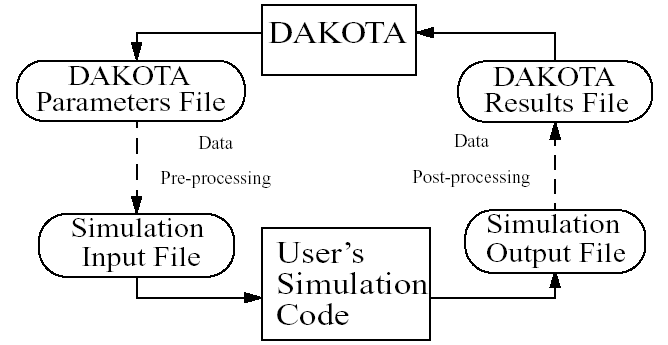
\includegraphics[scale=0.60]{images/dakota_flowchart}
  \caption{The loosely-coupled or ``black-box'' interface between
    Dakota and a user-supplied simulation code.}
  \label{introduction:bbinterface}
\end{figure}

The solid lines in Figure~\ref{introduction:bbinterface} denote file
input/output (I/O) operations that are part of Dakota or the user's
simulation code. The dotted lines indicate the passing/conversion of
information that must be implemented by the user. As Dakota runs, it
writes out a parameters file containing the current variable values.
Dakota then starts the user's simulation code (or, often, a short
driver script wrapping it), and when the simulation completes, reads
the response data from a results file. This process is repeated until
all of the simulation code runs required by the iterative study are
complete.

In some cases it is advantageous to have a close coupling between
Dakota and the simulation code. This close coupling is an advanced
feature of Dakota and is accomplished through either a direct
interface or a SAND (simultaneous analysis and design) interface. For
the direct interface, the user's simulation code is modified to behave
as a function or subroutine under Dakota. This interface can be
considered to be ``semi-intrusive'' in that it requires relatively
minor modifications to the simulation code. Its major advantage is the
elimination of the overhead resulting from file I/O and process
creation. It can also be a useful tool for parallel processing, by
encapsulating everything within a single executable. A SAND interface
approach is ``fully intrusive'' in that it requires further
modifications to the simulation code so that an optimizer has access
to the internal residual vector and Jacobian matrices computed by the
simulation code. In a SAND approach, both the optimization method and
a nonlinear simulation code are converged simultaneously. While this
approach can greatly reduce the computational expense of optimization,
considerable software development effort must be expended to achieve
this intrusive coupling between SAND optimization methods and the
simulation code.  SAND may be supported in future Dakota releases.

\section{Background and Mathematical Formulations}\label{introduction:background}

This section provides a basic introduction to the mathematical
formulation of optimization, nonlinear least squares, sensitivity
analysis, design of experiments, and uncertainty quantification
problems. The primary goal of this section is to introduce terms
relating to these topics, and is not intended to be a description of
theory or numerical algorithms. There are numerous sources of
information on these topics
(\cite{Aro89},~\cite{Gil81},~\cite{Haf92},~\cite{Hal00},~\cite{Noc99},~\cite{Van84}) and
the interested reader is advised to consult one or more of these
texts.

\subsection{Optimization}\label{introduction:background:optimization}

A general optimization problem is formulated as follows:

\begin{eqnarray}
  \hbox{minimize:} & & f(\mathbf{x})\nonumber\\
  & & \mathbf{x} \in \Re^{n}\nonumber\\
  \hbox{subject to:} & &
  \mathbf{g}_{L} \leq \mathbf{g(x)} \leq \mathbf{g}_U\nonumber\\
  & & \mathbf{h(x)}=\mathbf{h}_{t}\label{introduction:equation01}\\
  & & \mathbf{a}_{L} \leq \mathbf{A}_i\mathbf{x} \leq
  \mathbf{a}_U\nonumber\\
  & & \mathbf{A}_{e}\mathbf{x}=\mathbf{a}_{t}\nonumber\\
  & & \mathbf{x}_{L} \leq \mathbf{x} \leq \mathbf{x}_U\nonumber
\end{eqnarray}

where vector and matrix terms are marked in bold typeface. In this
formulation, $\mathbf{x}=[x_{1},x_{2},\ldots,x_{n}]$ is an
n-dimensional vector of real-valued \emph{design variables} or
\emph{design parameters}. The n-dimensional vectors, $\mathbf{x}_{L}$
and $\mathbf{x}_U$, are the lower and upper bounds, respectively, on
the design parameters. These bounds define the allowable values for
the elements of $\mathbf{x}$, and the set of all allowable values is
termed the \emph{design space} or the \emph{parameter space}. A
\emph{design point} or a \emph{sample point} is a particular set of 
values within the parameter space.

The optimization goal is to minimize the \emph{objective function},
$f(\mathbf{x})$, while satisfying the constraints.  Constraints can be
categorized as either linear or nonlinear and as either inequality or
equality. The \emph{nonlinear inequality constraints},
$\mathbf{g(x)}$, are ``2-sided,'' in that they have both lower and
upper bounds, $\mathbf{g}_L$ and $\mathbf{g}_U$, respectively. The
\emph{nonlinear equality constraints}, $\mathbf{h(x)}$, have target
values specified by $\mathbf{h}_{t}$.  The linear inequality
constraints create a linear system $\mathbf{A}_i\mathbf{x}$, where
$\mathbf{A}_i$ is the coefficient matrix for the linear system.  These
constraints are also 2-sided as they have lower and upper bounds,
$\mathbf{a}_L$ and $\mathbf{a}_U$, respectively. The linear equality
constraints create a linear system $\mathbf{A}_e\mathbf{x}$, where
$\mathbf{A}_e$ is the coefficient matrix for the linear system and
$\mathbf{a}_{t}$ are the target values.  The constraints partition the
parameter space into feasible and infeasible regions. A design point
is said to be \emph{feasible} if and only if it satisfies all of the
constraints. Correspondingly, a design point is said to be
\emph{infeasible} if it violates one or more of the constraints.

Many different methods exist to solve the optimization problem given
by Equation~\ref{introduction:equation01}, all of which iterate on
$\mathbf{x}$ in some manner.  That is, an initial value for each
parameter in $\mathbf{x}$ is chosen, the \emph{response quantities},
$f(\mathbf{x})$, $\mathbf{g(x)}$, $\mathbf{h(x)}$, are computed, often
by running a simulation, and some algorithm is applied to generate a
new $\mathbf{x}$ that will either reduce the objective function,
reduce the amount of infeasibility, or both.  To facilitate a general
presentation of these methods, three criteria will be used in the
following discussion to differentiate them: optimization problem type,
search goal, and search method.

The {\bf optimization problem type} can be characterized both by
the types of constraints present in the problem and by the linearity
or nonlinearity of the objective and constraint functions. For
constraint categorization, a hierarchy of complexity exists for
optimization algorithms, ranging from simple bound constraints,
through linear constraints, to full nonlinear constraints. By the
nature of this increasing complexity, optimization problem
categorizations are inclusive of all constraint types up to a
particular level of complexity. That is, an \emph{unconstrained
  problem} has no constraints, a \emph{bound-constrained problem} has
only lower and upper bounds on the design parameters, a
\emph{linearly-constrained problem} has both linear and bound
constraints, and a \emph{nonlinearly-constrained problem} may contain
the full range of nonlinear, linear, and bound constraints. If all of
the linear and nonlinear constraints are equality constraints, then
this is referred to as an \emph{equality-constrained problem}, and if
all of the linear and nonlinear constraints are inequality
constraints, then this is referred to as an
\emph{inequality-constrained problem}. Further categorizations can be
made based on the linearity of the objective and constraint functions.
A problem where the objective function and all constraints are linear
is called a \emph{linear programming (LP) problem}. These types of
problems commonly arise in scheduling, logistics, and resource
allocation applications. Likewise, a problem where at least some of
the objective and constraint functions are nonlinear is called a
\emph{nonlinear programming (NLP) problem}. These NLP problems
predominate in engineering applications and are the primary focus of
Dakota.

The {\bf search goal} refers to the ultimate objective of the
optimization algorithm, i.e., either global or local optimization. In
\emph{global optimization}, the goal is to find the design point that
gives the lowest feasible objective function value over the entire
parameter space. In contrast, in \emph{local optimization}, the goal
is to find a design point that is lowest relative to a ``nearby''
region of the parameter space. In almost all cases, global
optimization will be more computationally expensive than local
optimization. Thus, the user must choose an optimization algorithm
with an appropriate search scope that best fits the problem goals and
the computational budget.

The {\bf search method} refers to the approach taken in the
optimization algorithm to locate a new design point that has a lower
objective function or is more feasible than the current design point.
The search method can be classified as either \emph{gradient-based} or
\emph{nongradient-based}. In a gradient-based algorithm, gradients of
the response functions are computed to find the direction of
improvement.  Gradient-based optimization is the search method that
underlies many efficient local optimization methods. However, a
drawback to this approach is that gradients can be computationally
expensive, inaccurate, or even nonexistent. In such situations,
nongradient-based search methods may be useful. There are numerous
approaches to nongradient-based optimization. Some of the more well
known of these include pattern search methods (nongradient-based local
techniques) and genetic algorithms (nongradient-based global
techniques).  Because of the computational cost of running simulation
models, surrogate-based optimization (SBO) methods are often used to
reduce the number of actual simulation runs. In SBO, a surrogate or
approximate model is constructed based on a limited number of
simulation runs.  The optimization is then performed on the surrogate
model.  Dakota has an extensive framework for managing a variety of
local, multipoint, global, and hierarchical surrogates for use in
optimization.

The overview of optimization methods presented above underscores that
there is no single optimization method or algorithm that works best
for all types of optimization problems. Chapter~\ref{usage} provides
some guidelines on choosing which Dakota optimization algorithm is
best matched to your specific optimization problem.

\subsection{Nonlinear Least Squares for Parameter Estimation}\label{introduction:background:nonlinear}

Specialized least squares solution algorithms can exploit the
structure of a sum of the squares objective function for problems of
the form:

\begin{eqnarray}
  \hbox{minimize:} & & f(\mathbf{x}) =
  \sum_{i=1}^{n}[T_i(\mathbf{x})]^2\nonumber\\
  & & \mathbf{x} \in \Re^{n}\nonumber\\
  \hbox{subject to:} & &
  \mathbf{g}_L \leq \mathbf{g(x)} \leq \mathbf{g}_U\nonumber\\
  & & \mathbf{h(x)}=\mathbf{h}_{t}\label{introduction:equation02}\\
  & & \mathbf{a}_L \leq \mathbf{A}_i\mathbf{x} \leq
  \mathbf{a}_U\nonumber\\
  & & \mathbf{A}_e\mathbf{x}=\mathbf{a}_{t}\nonumber\\
  & & \mathbf{x}_L \leq \mathbf{x} \leq \mathbf{x}_U\nonumber
\end{eqnarray}

where $f(\mathbf{x})$ is the objective function to be minimized and
$T_i(\mathbf{x})$ is the i$^{\mathrm{th}}$ least squares term. The
bound, linear, and nonlinear constraints are the same as described
previously for (\ref{introduction:equation01}).  Specialized least
squares algorithms are generally based on the Gauss-Newton
approximation. When differentiating $f(\mathbf{x})$ twice, terms of
$T_i(\mathbf{x})T''_i(\mathbf{x})$ and $[T'_i(\mathbf{x})]^{2}$
result. By assuming that the former term tends toward zero near the
solution since $T_i(\mathbf{x})$ tends toward zero, then the Hessian
matrix of second derivatives of $f(\mathbf{x})$ can be approximated
using only first derivatives of $T_i(\mathbf{x})$.  As a result,
Gauss-Newton algorithms exhibit quadratic convergence rates near the
solution for those cases when the Hessian approximation is accurate,
i.e. the residuals tend towards zero at the solution.  Thus, by
exploiting the structure of the problem, the second order convergence
characteristics of a full Newton algorithm can be obtained using only
first order information from the least squares terms.

A common example for $T_i(\mathbf{x})$ might be the difference
between experimental data and model predictions for a response
quantity at a particular location and/or time step, i.e.:

\begin{equation}
  T_i(\mathbf{x}) = R_i(\mathbf{x})-\overline{R_i}
  \label{introduction:equation03}
\end{equation}

where $R_i(\mathbf{x})$ is the response quantity predicted by the
model and $\overline{R_i}$ is the corresponding experimental data.
In this case, $\mathbf{x}$ would have the meaning of model parameters
which are not precisely known and are being calibrated to match
available data. This class of problem is known by the terms parameter
estimation, system identification, model calibration, test/analysis
reconciliation, etc.

\subsection{Sensitivity Analysis and Parameter Studies}\label{introduction:background:sensitivity}

In many engineering design applications, sensitivity analysis
techniques and parameter study methods are useful in identifying which
of the design parameters have the most influence on the response
quantities. This information is helpful prior to an optimization study
as it can be used to remove design parameters that do not strongly
influence the responses. In addition, these techniques can provide
assessments as to the behavior of the response functions (smooth or
nonsmooth, unimodal or multimodal) which can be invaluable in
algorithm selection for optimization, uncertainty quantification, and
related methods. In a post-optimization role, sensitivity information
is useful is determining whether or not the response functions are
robust with respect to small changes in the optimum design point.

In some instances, the term sensitivity analysis is used in a local
sense to denote the computation of response derivatives at a point.
These derivatives are then used in a simple analysis to make design
decisions. Dakota supports this type of study through numerical
finite-differencing or retrieval of analytic gradients computed within
the analysis code. The desired gradient data is specified in the
responses section of the Dakota input file and the collection of this
data at a single point is accomplished through a parameter study
method with no steps. This approach to sensitivity analysis should be
distinguished from the activity of augmenting analysis codes to
internally compute derivatives using techniques such as direct or
adjoint differentiation, automatic differentiation (e.g., ADIFOR), or
complex step modifications. These sensitivity augmentation activities
are completely separate from Dakota and are outside the scope of this
manual. However, once completed, Dakota can utilize these analytic
gradients to perform optimization, uncertainty quantification, and
related studies more reliably and efficiently.

In other instances, the term sensitivity analysis is used in a more
global sense to denote the investigation of variability in the
response functions. Dakota supports this type of study through
computation of response data sets (typically function values only, but
all data sets are supported) at a series of points in the parameter
space. The series of points is defined using either a vector, list,
centered, or multidimensional parameter study method. For example, a
set of closely-spaced points in a vector parameter study could be used
to assess the smoothness of the response functions in order to select
a finite difference step size, and a set of more widely-spaced points
in a centered or multidimensional parameter study could be used to
determine whether the response function variation is likely to be
unimodal or multimodal. See Chapter~\ref{ps} for additional
information on these methods. These more global approaches to
sensitivity analysis can be used to obtain trend data even in
situations when gradients are unavailable or unreliable, and they are
conceptually similar to the design of experiments methods and sampling
approaches to uncertainty quantification described in the following
sections.

\subsection{Design of Experiments}\label{introduction:background:design}

Classical design of experiments (DoE) methods and the more modern
design and analysis of computer experiments (DACE) methods are both
techniques which seek to extract as much trend data from a parameter
space as possible using a limited number of sample points. Classical
DoE techniques arose from technical disciplines that assumed some
randomness and nonrepeatability in field experiments (e.g.,
agricultural yield, experimental chemistry). DoE approaches such as
central composite design, Box-Behnken design, and full and fractional
factorial design generally put sample points at the extremes of the
parameter space, since these designs offer more reliable trend
extraction in the presence of nonrepeatability. DACE methods are
distinguished from DoE methods in that the nonrepeatability component
can be omitted since computer simulations are involved. In these
cases, space filling designs such as orthogonal array sampling and
Latin hypercube sampling are more commonly employed in order to
accurately extract trend information. Quasi-Monte Carlo sampling 
techniques which are constructed to fill the unit hypercube with 
good uniformity of coverage can also be used for DACE.

Dakota supports both DoE and DACE techniques. In common usage, only
parameter bounds are used in selecting the samples within the
parameter space. Thus, DoE and DACE can be viewed as special cases of
the more general probabilistic sampling for uncertainty quantification
(see following section), in which the DoE/DACE parameters are treated
as having uniform probability distributions. The DoE/DACE techniques
are commonly used for investigation of global response trends,
identification of significant parameters (e.g., main effects), and as
data generation methods for building response surface approximations.

\subsection{Uncertainty Quantification}\label{introduction:background:uncertainty}

Uncertainty quantification (UQ) is the process of determining the
effect of input uncertainties on response metrics of interest (forward
propagating uncertainties through the model).  These input
uncertainties may be characterized as either aleatory uncertainties,
which are irreducible variabilities inherent in nature, or epistemic
uncertainties, which are reducible uncertainties resulting from a lack
of knowledge.  Since sufficient data is generally available for
aleatory uncertainties, probabilistic methods are commonly used for
computing response distribution statistics based on input probability
distribution specifications.  Conversely, for epistemic uncertainties,
data is generally sparse, making the use of probability theory
questionable and leading to nonprobabilistic methods based on interval
specifications.

UQ is related to sensitivity analysis in that the common goal is to
gain an understanding of how variations in the parameters affect the
response functions of the engineering design problem. However, for UQ,
some or all of the components of the parameter vector, $\mathbf{x}$,
are considered to be uncertain as specified by particular probability
distributions (e.g., normal, exponential, extreme value).  By
assigning specific distributional structure to the inputs,
distributional structure for the outputs (i.e., response statistics)
can be inferred.

Current Dakota methods for modeling aleatory uncertainty include
sampling methods, local and global reliability methods, and stochastic
expansion methods (polynomial chaos expansions and stochastic
collocation).  Current methods for modeling epistemic uncertainties
include Dempster-Shafer theory of evidence and local or global
interval estimation.  The sampling, reliability, stochastic expansion,
Dempster-Shafer, and interval UQ approaches are described in more
detail in Chapter~\ref{uq}.  Current methods for modeling mixed
aleatory/epistemic uncertainties include interval-valued probability,
second-order probability, and Dempster-Shafer theory of evidence, as
described in Section~\ref{adv_models:mixed_uq}.

%The impact on the response functions due to the probabilistic nature
%of the parameters is often estimated using a sampling-based approach
%such as Monte Carlo sampling or one of its variants (latin hypercube,
%quasi-Monte Carlo, Markov-chain Monte Carlo, etc.). In these sampling
%approaches, a random number generator is used to select different
%values of the parameters with probability specified by their
%probability distributions. This is the point that distinguishes UQ
%sampling from DoE/DACE sampling, in that the former supports general
%probabilistic descriptions of the parameter set and the latter
%generally supports only a bounded parameter space description.  A
%particular set of parameter values is often called a \emph{sample
%point}, or simply a \emph{sample}. With Monte Carlo and Latin
%Hypercube sampling, the user may specify correlations among the input
%sample points. After a user-selected number of sample points has been
%generated, the response functions for each sample are evaluated. Then,
%a statistical analysis is performed on the response function values to
%yield information on their characteristics. While this approach is
%straightforward, and readily amenable to parallel computing, it can be
%computationally expensive depending on the accuracy requirements of
%the statistical information (which links directly to the number of
%sample points).

%Finally, when the input uncertainties are poorly characterized, then
%epistemic uncertainty methods, such as second-order probability or
%Dempster-Shafer theory of evidence, can be used to compute intervals
%of potential probability values.  The second-order probability
%approach performs an ensemble of aleatory UQ analyses, one for each
%realization of the epistemic parameter set.  The ensemble of CDF/CCDF
%curves generates what is known as a ``horse-tail'' plot.
%Dempster-Shafer, on the other hand, directly generates probability
%bounds, known as the belief and plausibility functions.


\section{Using this Manual}\label{introduction:using}

The previous sections in this chapter provide a brief overview of the
capabilities in Dakota, and introduce some of the common terms that
are used in the fields of optimization, parameter estimation,
sensitivity analysis, design of experiments, and uncertainty
quantification. A Dakota user new to these techniques and terms is
advised to consult the cited references to obtain more detailed
descriptions of methods and algorithms in these disciplines.

Chapter~\ref{tutorial} provides information on how to obtain, install,
and use Dakota. In addition, example problems are presented in this
tutorial chapter to demonstrate some of Dakota's capabilities for
parameter studies, optimization, and UQ. Chapter~\ref{capabilities}
provides a brief overview of all of the different software packages
and capabilities in Dakota. Chapters~\ref{ps} through~\ref{sbm}
provide details on the iterative algorithms supported in Dakota,
Chapters~\ref{models} through~\ref{responses} provide information on
model components which are involved in parameter to response mappings,
and Chapters~\ref{input} and~\ref{output} describe the inputs to and
outputs from Dakota.  Several advanced topics are covered next, with
Chapter~\ref{strat} on strategies, Chapter~\ref{adv_models} on model
recursions, Chapter~\ref{advint} on interfacing Dakota with
engineering simulation codes, and Chapter~\ref{parallel} on Dakota's
parallel computing capabilities.  Next, Chapter~\ref{usage} provides
some usage guidelines for selecting from among Dakota's different
algorithms for solving particular classes of problems.  Finally,
Chapter~\ref{restart} through Chapter~\ref{additional} describe
restart utilities, failure capturing facilities, and additional test
problems, respectively.

\chapter{DAKOTA Tutorial}\label{tutorial}

\section{Getting Started}\label{tutorial:installation}

DAKOTA operates on most systems running Unix or Linux operating
systems as well as on Windows with the help of a MinGW or Cygwin
emulation layer.  DAKOTA is developed and most extensively tested on
Redhat Enterprise Linux with GNU compilers, but additional operating
systems / compiler combinations are tested nightly as well.  See the
DAKOTA website for more information on supported platforms for
particular DAKOTA versions.

Department of Energy users: DAKOTA may already be available on your
target system. Sandia users should visit
\url{http://dakota.sandia.gov/sandia_only/} for information on
supported DAKOTA installations on engineering networks and cluster
computers, as well as for Sandia-specific downloads.  At other DOE
institutions, contact your system administrator about DAKOTA
availability.  If not available for your target platform, you may
still download DAKOTA as described below.

\subsection {Quickstart}\label{tutorial:installation:quickstart}

Getting started with DAKOTA typically involves the following steps:
\begin{itemize}
  \item Download DAKOTA: binary executables and source code are
    available from\\
    \url{http://dakota.sandia.gov/}.

  \item After downloading, unpack the files, yielding a {\tt Dakota/}
    directory.  For tar.gz or .tgz files, e.g.,\\
    \texttt{Dakota\_5\_x.OSversion.tar.gz} either invoke
    \begin{small}
\begin{verbatim}
    gunzip Dakota_5_x.OSversion.tar.gz
    tar -xvf Dakota_5_x.OSversion.tar
\end{verbatim}
    \end{small}
    or (slightly faster and less demanding of disk space) invoke
    \begin{small}
\begin{verbatim}
    gzip -dc Dakota_5_x.OSversion.tar.gz | tar xf -
\end{verbatim}
    \end{small}
    A similar process applies to windows distributions which are
    packaged as .zip files.  These can be extracted with the Windows
    extractor or WinZIP, for example.

  \item For binary packages, {\tt Dakota/bin} contains executable
    files. Example input files and interfaces are in
    \texttt{Dakota/examples} (see \texttt{Dakota/examples/README}) and
    \texttt{Dakota/test}.  To get started, open a terminal shell or
    Command Prompt and set your PATH to include {\tt Dakota/bin} (and
    optionally DAKOTA's test or example directories).  On Linux:
    \begin{small}
\begin{verbatim}
    export PATH=/path/to/Dakota/bin:$PATH
\end{verbatim} %$
    \end{small}
    or on Windows:
    \begin{small}
\begin{verbatim}
    set PATH=C:\path\to\Dakota\bin:%PATH%
\end{verbatim}
    \end{small}
    then proceed with running as described below in 
    Section~\ref{tutorial:installation:running}.

  \item For source packages, configure and compile using either GNU
    configure/make or CMake/make.  For example, for configure:
    \begin{small}
\begin{verbatim}
    cd Dakota/
    configure
    make
    make install  # optional
\end{verbatim}
    \end{small}
    or for CMake
    \begin{small}
\begin{verbatim}
    cd Dakota/
    mkdir build && cd build/
    cmake ..
    make
    make install  # optional
\end{verbatim}
    \end{small}
    Detailed configuration options are available on the DAKOTA
    website, including the Developer Portal
    \url{http://dakota.sandia.gov/developer/}.
    
  \item Verify that DAKOTA runs; see
    Section~\ref{tutorial:installation:running}

  \item Joining mailing lists and get help: the most up to date
    guidance for downloading, compiling, installing, or running
    DAKOTA, or seeking help is available on the DAKOTA website \\
    (\url{http://dakota.sandia.gov/resources.html}). In addition,
    guidance is also included in files included with DAKOTA, including
    \texttt{Dakota/INSTALL}. Further platform/operating
    system-specific guidance can be found in {\tt
    Dakota/examples/platforms}.  For getting started on Windows, see
    the files \texttt{INSTALL.cygwin} and \texttt{INSTALL.mingw} in
    \texttt{Dakota/examples/platforms}.
\end{itemize}


\subsection{Running DAKOTA}\label{tutorial:installation:running}

The DAKOTA executable file is named {\tt dakota} ({\tt dakota.exe} on
Windows). If this command is entered at the command prompt without any
arguments, a usage message similar to the following appears:
\begin{small}
\begin{verbatim}
usage: dakota [options and <args>]
        -help (Print this summary)
        -version (Print DAKOTA version number)
        -input <$val> (REQUIRED DAKOTA input file $val)
        -output <$val> (Redirect DAKOTA standard output to file $val)
        -error <$val> (Redirect DAKOTA standard error to file $val)
        -parser <$val> (Parsing technology: nidr[strict][:dumpfile])
	-no_input_echo (Do not echo DAKOTA input file)
	-check (Perform input checks)
        -pre_run [$val] (Perform pre-run (variables generation) phase)
        -run [$val] (Perform run (model evaluation) phase)
        -post_run [$val] (Perform post-run (final results) phase)
        -read_restart [$val] (Read an existing DAKOTA restart file $val)
        -stop_restart <$val> (Stop restart file processing at evaluation $val)
        -write_restart [$val] (Write a new DAKOTA restart file $val)
\end{verbatim}
\end{small}
%$ this comment is here to trick xemacs into highlighting syntax correctly

Of these available command line inputs, only the ``\texttt{-input}''
option is required, and ``\texttt{-input}'' can be omitted if the
input file name is the final item on the command line; all other
command-line inputs are optional. The ``\texttt{-help}'' option prints
the usage message above. The ``\texttt{-version}'' option prints the
version number of the executable. The ``\texttt{-check}'' option
invokes a dry-run mode in which the input file is processed and
checked for errors, but the study is not performed. The
``\texttt{-input}'' option provides the name of the DAKOTA input file.
The ``\texttt{-output}'' and ``\texttt{-error}'' options provide file
names for redirection of the DAKOTA standard output (stdout) and
standard error (stderr), respectively.  By default, DAKOTA will echo
the input file to the output stream, but ``\texttt{-no_input_echo}''
can override this behavior.

The ``\texttt{-parser}'' input
is for debugging and will not be further described here.  The
``\texttt{-read\_restart}'' and ``\texttt{-write\_restart}'' command
line inputs provide the names of restart databases to read from and
write to, respectively. The ``\texttt{-stop\_restart}'' command line
input limits the number of function evaluations read from the restart
database (the default is all the evaluations) for those cases in which
some evaluations were erroneous or corrupted. Restart management is an
important technique for retaining data from expensive engineering
applications. This advanced topic is discussed in detail in
Chapter~\ref{usage}. Note that these command line inputs can be
abbreviated so long as the abbreviation is unique, so the following
are valid, unambiguous specifications: ``\texttt{-h}'',
``\texttt{-v}'', ``\texttt{-c}'', ``\texttt{-i}'', ``\texttt{-o}'',
``\texttt{-e}'', ``\texttt{-re}'', ``\texttt{-s}'', ``\texttt{-w}'',
``\texttt{-pr}'', ``\texttt{-ru}'', and ``\texttt{-po}'' and can be
used in place of the longer forms of the command line inputs.

To run DAKOTA with a particular input file, the following syntax can
be used:
\begin{small}
\begin{verbatim}
    dakota -i dakota.in
\end{verbatim}
\end{small}
or more simply
\begin{small}
\begin{verbatim}
    dakota dakota.in
\end{verbatim}
\end{small}

This will echo the standard output (stdout) and standard error
(stderr) messages to the terminal. To redirect stdout and stderr to
separate files, the \texttt{-o} and \texttt{-e} command line options
may be used:
\begin{small}
\begin{verbatim}
    dakota -i dakota.in -o dakota.out -e dakota.err
\end{verbatim}
\end{small}
or
\begin{small}
\begin{verbatim}
    dakota -o dakota.out -e dakota.err dakota.in
\end{verbatim}
\end{small}

Alternatively, any of a variety of Unix redirection variants can be
used. The simplest of these redirects stdout to another file:
\begin{small}
\begin{verbatim}
    dakota dakota.in > dakota.out
\end{verbatim}
\end{small}

To append to a file rather than overwrite it, ``\texttt{>>}'' is used
in place of ``\texttt{>}''. The syntax to redirect stderr as well as stdout
to the same file depends on the shell you are using.  With csh, simply append
``\texttt{\&}'' with no embedded space, i.e.,
``\texttt{>\&}'' or ``\texttt{>>\&}''. With the Bourne shell (sh or bash) use
``\texttt{>dakota.out 2>\&1}'' or ``\texttt{>>dakota.out 2>\&1}''.
With csh, if you have the noclobber environment variable set but
wish either to overwrite an existing output file or to append to a file that
does not yet exist, append ``\texttt{!}'' to the redirection operators
(with no intervening spaces), i.e.,
``\texttt{>!}'', ``\texttt{>\&!}'', ``\texttt{>>!}'', or
``\texttt{>>\&!}''.

To run the dakota process in the background, append an ampersand
symbol (\&) to the command with an embedded space, e.g.,
\begin{small}
\begin{verbatim}
    dakota dakota.in > dakota.out &
\end{verbatim}
\end{small}

Refer to~\cite{And86} for more information on Unix redirection and
background commands.

The ``\texttt{-pre\_run}'', ``\texttt{-run}'', and
``\texttt{-post\_run}'' switches instruct DAKOTA to run one or more
execution phases, excluding others.  For example pre-run might
generate variable sets, run (core run) invoke the simulation to
evaluate variables, producing responses, and post-run accepts
variable/response sets and analyzes the results (for example,
calculate correlations from a set of samples).  Currently only two
modes are supported and only for sampling, parameter study, and DACE
methods: (1) pre-run only with optional tabular output of variables:
\begin{small}
\begin{verbatim}
    dakota -i dakota.in -pre_run [::myvariables.dat]
\end{verbatim}
\end{small}
and (2) post-run only with required tabular input of variables/responses:
\begin{small}
\begin{verbatim}
    dakota -i dakota.in -post_run myvarsresponses.dat::
\end{verbatim}
\end{small}

 
\section{Rosenbrock and Textbook Test Problems}\label{tutorial:rosenbrock}

Many of the example problems in this chapter use the Rosenbrock
function \cite{Rosenbrock60} (also described in \cite{Gil81}, among
other places), which has the form:

\begin{equation}
f(x_1,x_2)=100(x_2-x_1^2)^2+(1-x_1)^2 \label{tutorial:rosen}
\end{equation}

A three-dimensional plot of this function is shown in
Figure~\ref{tutorial:rosenbrock_prob}(a), where both $x_1$ and
$x_2$ range in value from $-2$ to $2$.
Figure~\ref{tutorial:rosenbrock_prob}(b) shows a contour plot
for Rosenbrock's function. An optimization problem using Rosenbrock's
function is formulated as follows:

\begin{eqnarray}
\texttt{minimize }   & & f(x_1,x_2)          \nonumber\\
                     & & \mathbf{x} \in \Re^2\nonumber\\
\texttt{subject to } & & -2 \le x_1 \le 2    \\
                     & & -2 \le x_2 \le 2    \nonumber
\end{eqnarray}

\begin{figure}[htp!]
  \centering
  \begin{tabular}{cc}
  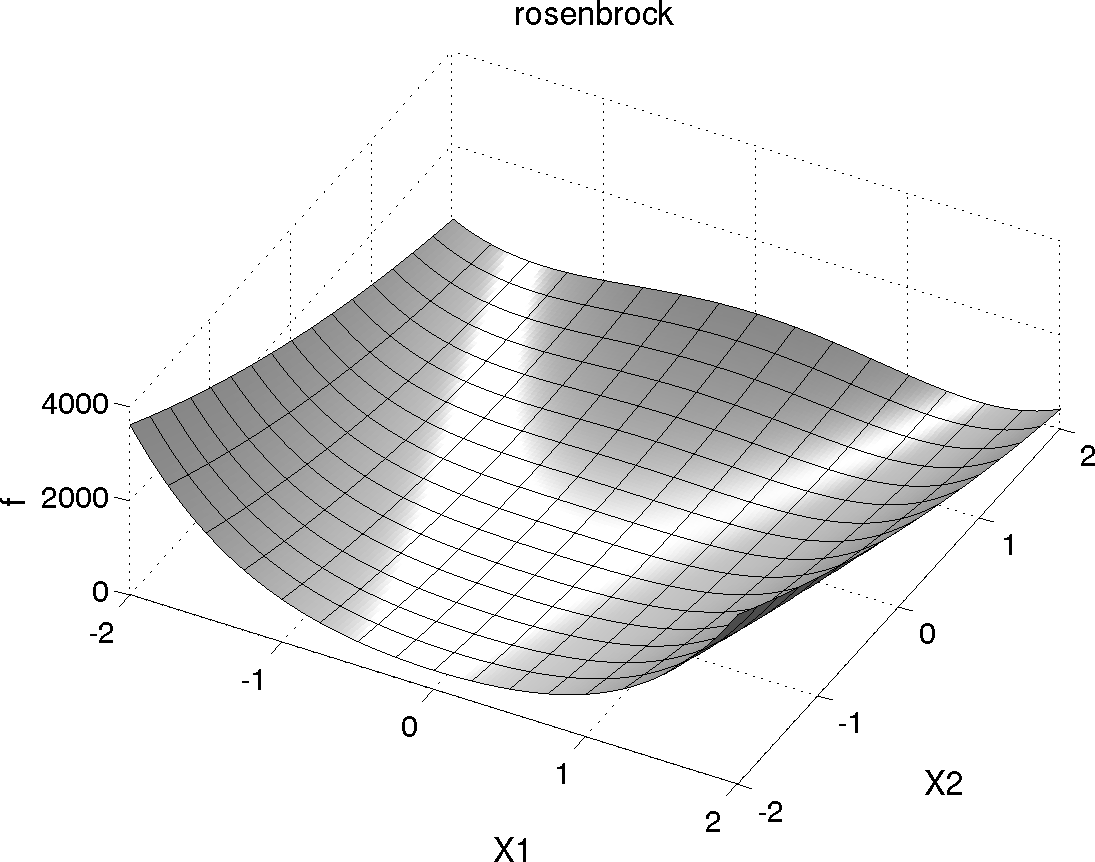
\includegraphics[height=2.5in]{images/rosen_3d_surf} &
  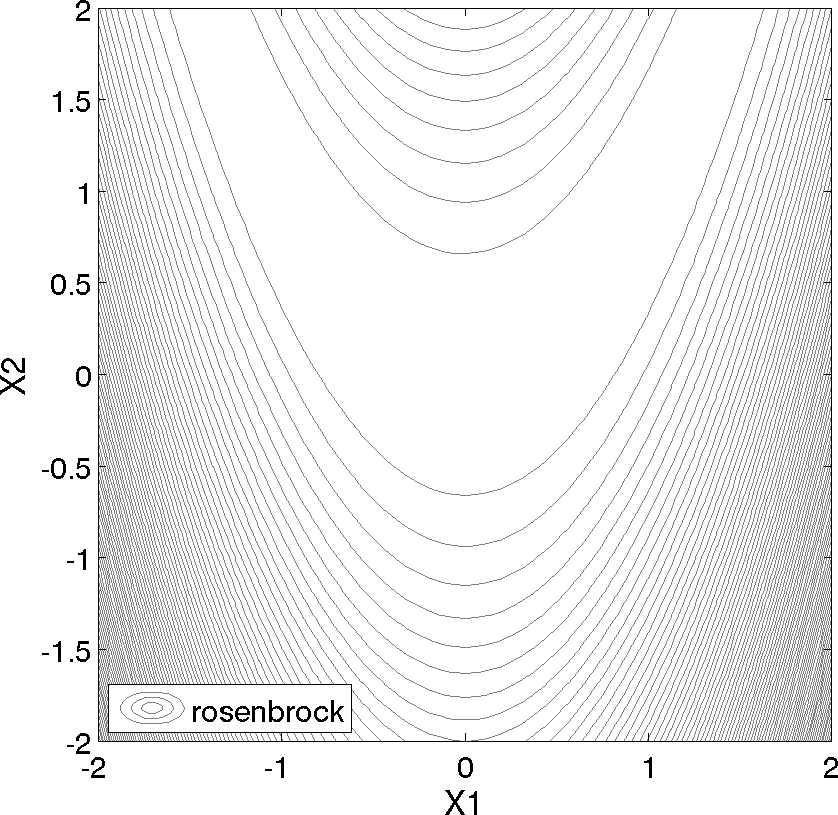
\includegraphics[height=2.5in]{images/rosen_2d_surf} \\
  (a) & (b) \\
  \end{tabular}
  \caption{Rosenbrock's function: (a) 3-D plot and (b) contours with
  $x_1$ on the bottom axis.}
  \label{tutorial:rosenbrock_prob}
\end{figure}

Note that there are no linear or nonlinear constraints in this
formulation, so this is a bound constrained optimization problem. The
unique solution to this problem lies at the point
$(x_1,x_2) = (1,1)$, where the function value is zero.

The two-variable version of the ``textbook'' example problem provides
a nonlinearly constrained optimization test case. It is formulated as:
\begin{eqnarray}
\texttt{minimize }
& & f = (x_1-1)^{4}+(x_2-1)^{4}     \nonumber \\
\texttt{subject to }
& & g_1 = x_1^2-\frac{x_2}{2} \le 0 \nonumber \\
& & g_2 = x_2^2-\frac{x_1}{2} \le 0 \label{tutorial:textbook_f} \\
& &  0.5 \le x_1 \le 5.8            \nonumber \\
& & -2.9 \le x_2 \le 2.9            \nonumber
\end{eqnarray}

Contours of this example problem are illustrated in
Figure~\ref{tutorial:textbook_prob}(a), with a close-up view of
the feasible region given in
Figure~\ref{tutorial:textbook_prob}(b).

\begin{figure}[htp!]
  \centering
  \begin{tabular}{cc}
  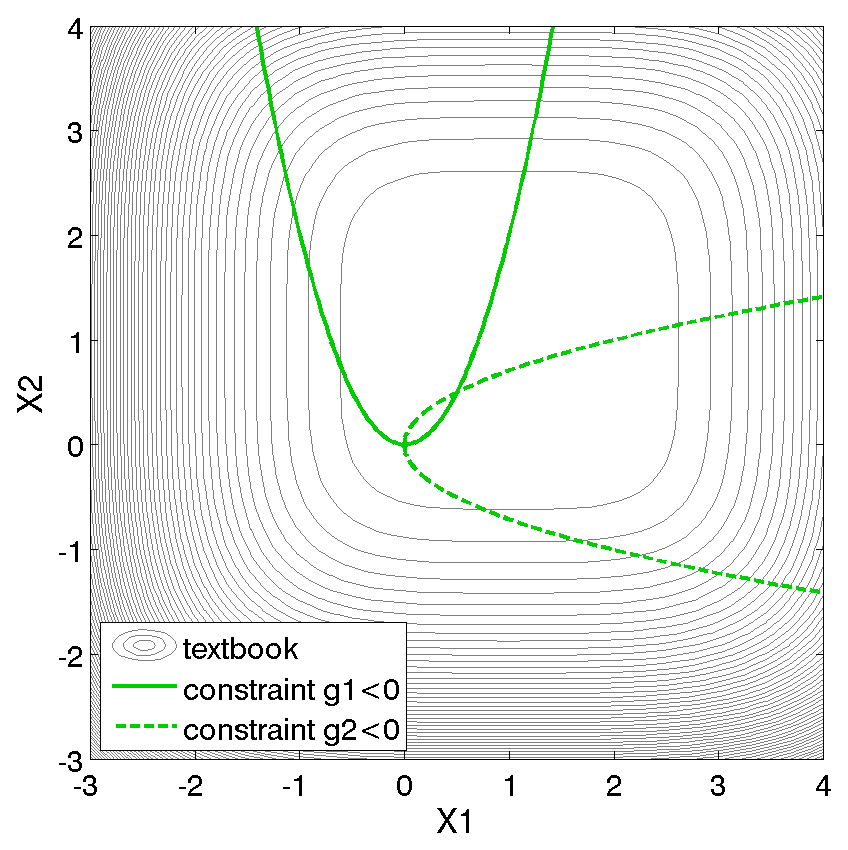
\includegraphics[height=2.5in]{images/textbook_contours} &
  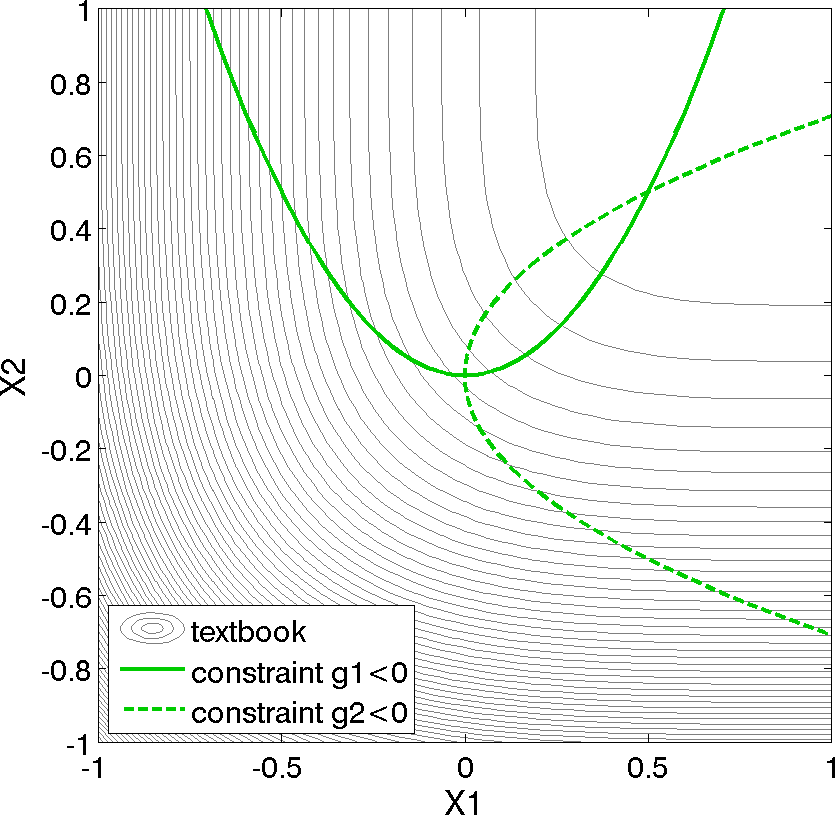
\includegraphics[height=2.5in]{images/textbook_closeup} \\
  (a) & (b) \\
  \end{tabular}
  \caption{Contours of the textbook problem (a) on the $[-3,4] \times
    [-3,4]$ domain and (b) zoomed into an area containing the
    constrained optimum point $(x_1,x_2) = (0.5,0.5)$. The
    feasible region lies at the intersection of the two constraints
    $g_1$ (solid) and $g_2$ (dashed).}
  \label{tutorial:textbook_prob}
\end{figure}

For the textbook example problem, the unconstrained minimum occurs at
$(x_1,x_2) = (1,1)$. However, the inclusion of the constraints
moves the minimum to $(x_1,x_2) = (0.5,0.5)$.

Several other example problems are available. See
Chapter~\ref{additional} for a description of these example problems
as well as further discussion of the Rosenbrock and textbook example
problems.

\section{DAKOTA Input File Format}\label{tutorial:dakota}

All of the DAKOTA input files for the simple example problems
presented here are included in the distribution tar files within
directory \texttt{Dakota/examples/tutorial}. A simple DAKOTA
input file (that is named \texttt{dakota\_rosenbrock\_2d.in})
for a two-dimensional parameter study on Rosenbrock's
function is shown in Figure~\ref{tutorial:rosenbrock_2d}.
This input file will be used to
describe the basic format and syntax used in all DAKOTA input files.

\begin{figure}[ht!]
  \centering
  \begin{bigbox}
    \begin{small}
      \verbatimtabinput[8]{dakota_rosenbrock_2d.in}
    \end{small}
  \end{bigbox}
  \caption{Rosenbrock 2-D parameter study example: the DAKOTA input
    file.}
  \label{tutorial:rosenbrock_2d}
\end{figure}

There are six specification blocks that may appear in DAKOTA input
files. These are identified in the input file using the following
keywords: variables, interface, responses, model, method, and strategy. These
keyword blocks can appear in any order in a DAKOTA input file. At
least one \emph{variables}, \emph{interface}, \emph{responses}, and
\emph{method} specification must appear, and no more than one
\emph{strategy} specification should appear. In Figure~
\ref{tutorial:rosenbrock_2d}, one of each of the keyword blocks is
used.  Additional syntax features include use of the \#
symbol to indicate a comment, use of single or double quotes for string inputs
(e.g., \texttt{'x1'}), the use of commas and/or white space for separation of
specifications, and the optional use of ``='' symbols to indicate
supplied data. See the DAKOTA Reference
Manual~\cite{RefMan} for additional details on this input file syntax.

The first section of the input file shown in
Figure~\ref{tutorial:rosenbrock_2d} is the \emph{strategy} section.
This keyword section is used to specify some of DAKOTA's advanced
meta-procedures such as hybrid optimization, 
multi-start optimization, and Pareto optimization.
See Chapter~\ref{strat} for more information on these
meta-procedures. The \emph{strategy} section also contains the
settings for DAKOTA's graphical output (via the \texttt{graphics}
flag) and the tabular data output (via the
\texttt{tabular\_graphics\_data} keyword).

The \emph{method} section of the input file specifies the iterative
technique that DAKOTA will employ, such as a parameter study,
optimization method, data sampling technique, etc.
The keyword \texttt{multidim\_parameter\_study}
in Figure~\ref{tutorial:rosenbrock_2d} calls for a multidimensional
parameter study, while the keyword \texttt{partitions} specifies the
number of intervals per variable. In this case, there will be eight
intervals (nine data points) evaluated between the lower and upper
bounds of both variables (bounds provided subsequently in the
\emph{variables} section), for a total of 81 response function
evaluations.

The \emph{model} section of the input file specifies the model that
DAKOTA will use.  A model provides the logical unit for determining
how a set of variables is mapped into a set of responses in support of
an iterative method.  The model allows one to specify a single
interface, or to manage more sophisticated mappings involving
surrogates or nested iteration.  For example, one might want to use
an approximate model for optimization or uncertainty quantification,
due to the lower computational cost.  The
\texttt{model} keyword allows one to specify if the iterator will be
operating on a data fit surrogate (such as a polynomial regression,
neural net, etc.), a hierarchical surrogate (which uses the corrected
results of a lower fidelity simulation model as an approximation to a
higher fidelity simulation), or a nested model. See
Chapter~\ref{models} for additional model specification details. If
these advanced facilities for surrogate modeling or nested iteration
are not required, then it is not necessary to specify the
\texttt{model} keyword at all, since the default behavior is the use
of a ``single'' model constructed with the last set of responses,
variables, and interface specified.  In
Figure~\ref{tutorial:rosenbrock_2d}, the keyword \texttt{single}
explicitly specifies the use of a single model in the parameter study,
even though this is the default.

The \emph{variables} section of the input file specifies the
characteristics of the parameters that will be used in the problem
formulation. The variables can be continuous or discrete, and can be
classified as design variables, uncertain variables, or state
variables. See Chapter~\ref{variables} for more information on the
types of variables supported by DAKOTA.  The \emph{variables} section
shown in Figure~\ref{tutorial:rosenbrock_2d} specifies that there are
two continuous design variables.  The sub-specifications for
continuous design variables
% use the abbreviation ``cdv'' in the input file and
provide the descriptors ``x1'' and ``x2'' as well as lower
and upper bounds for these variables. The information about the
variables is organized in column format for readability. So, both
variables $x_1$ and $x_2$ have a lower bound of -2.0 and an upper
bound of 2.0.

The \emph{interface} section of the input file specifies what approach
will be used to map variables into responses as well as details on how
DAKOTA will pass data to and from a simulation code.
In this example, the keyword \texttt{direct} is used to indicate the
use of a function linked directly into DAKOTA.
Alternatively, \texttt{fork} or \texttt{system} executions can be used
to invoke instances of a simulation code that is external to DAKOTA,
as explained in Section \ref{tutorial:example:user_supply:optimization2} 
and Chapter~\ref{advint}.
The \texttt{analysis\_driver} keyword indicates the name of the test
function.  With \texttt{fork} or \texttt{system}, default file names
would be used for passing data between DAKOTA and the simulation code.

The \emph{responses} section of the input file specifies the types of
data that the interface will return to DAKOTA. For the example shown
in Figure~\ref{tutorial:rosenbrock_2d}, the assignment
\texttt{num\_objective\_functions = 1}
indicates that there is only one objective
function.  Since there are no constraints
associated with Rosenbrock's function, the keywords for
constraint specifications are omitted. The keywords
\texttt{no\_gradients} and \texttt{no\_hessians} indicate that no
derivatives will be provided to the method; none are needed for
a parameter study.

\section{Example Problems}\label{tutorial:example}

This section serves to familiarize users about how to perform parameter 
studies, optimization, and uncertainty quantification through their common
DAKOTA interface.  The initial examples utilize simple built in driver 
functions; later we show how to utilize DAKOTA to drive the evaluation of 
user supplied black box code.  The examples presented in this chapter 
are intended to show the simplest use of DAKOTA for several methods of 
each type.  More advanced examples of using DAKOTA for specific purposes 
are provided in subsequent, topic-based, chapters.

\subsection{Parameter Studies}\label{tutorial:example:param_study}

Parameter study methods in the DAKOTA toolkit involve the computation 
of response data sets at a selection of points in the parameter space. 
These response data sets are not linked to any specific interpretation,
so they may consist of any allowable specification from the responses 
keyword block, i.e., objective and constraint functions, least squares 
terms and constraints, or generic response functions. This allows the 
use of parameter studies in direct coordination with optimization, least 
squares, and uncertainty quantification studies without significant
modification to the input file.  
The two examples given in this subsection are for a two-dimensional 
tensor product of sample points and a vector parameter study.

\subsubsection{Two-Dimensional Grid Parameter Study}\label{tutorial:example:param_study:two}

The 2-D parameter study example problem listed in Figure~
\ref{tutorial:rosenbrock_2d} is executed by DAKOTA using the
following command:
\begin{small}
\begin{verbatim}
    dakota dakota_rosenbrock_2d.in > 2d.out
\end{verbatim}
\end{small}

The output of the DAKOTA run is directed to the file named
\texttt{2d.out}. For comparison, a file named \texttt{2d.out.sav} is
included in the \texttt{Dakota/examples/tutorial} directory. As
for many of the examples, DAKOTA provides a report on the best design
point located during the study at the end of these output files.

This 2-D parameter study produces the grid of data samples shown in
Figure~\ref{tutorial:rosenbrock_2d_graphics}. In general, a multidimensional 
parameter study lets one generate a grid in multiple dimensions. 
The keyword \texttt{multidim\_parameter\_study} indicates that 
a grid will be generated over all variables.  The keyword 
\texttt{partitions} indicates the number of grid partitions in 
each dimension. For this example, the number of the grid partitions 
are the same in each dimension (8 partitions) but it would be possible 
to specify (partitions = 8 2), and have only two partitions 
over the second input variable.   Note that the
\texttt{graphics} flag in the \emph{strategy} section of the input
file could be commented out since, for this example, the iteration
history plots created by DAKOTA are not particularly instructive. More
interesting visualizations can be created by importing DAKOTA's
tabular data into an external graphics/plotting package. Common
graphics and plotting packages include Mathematica, Matlab, Microsoft
Excel, Origin, Tecplot, and many others. (Sandia National Laboratories
and the DAKOTA developers do not endorse any of these commercial
products.)

\begin{figure}[htb!]
  \centering
  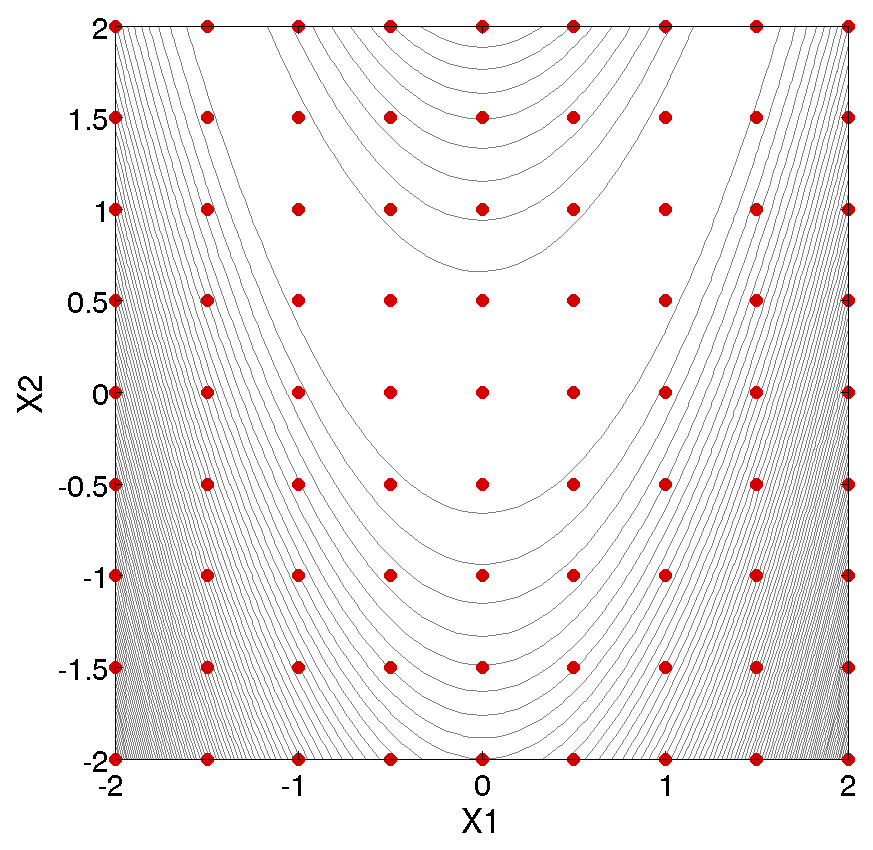
\includegraphics[height=2.5in]{images/rosen_2d_pts}
  \caption{Rosenbrock 2-D parameter study example:
  location of the design points (dots) evaluated.}
  \label{tutorial:rosenbrock_2d_graphics}
\end{figure}

\subsubsection{Vector Parameter Study}\label{tutorial:example:param_study:vector}

In addition to the multidimensional parameter study, DAKOTA can
perform a vector parameter study, i.e., a parameter study between any
two design points in an \emph{n}-dimensional parameter space.

An input file for the vector parameter study is shown in Figure~
\ref{tutorial:rosenbrock_vector}.  The primary differences
between this input file and the previous input file are found in the
\emph{variables} and \emph{method} sections. In the variables section,
the keywords for the bounds are removed and replaced with the keyword
\texttt{initial\_point} that specifies the starting point for the
parameter study. In the method section, the
\texttt{vector\_parameter\_study} keyword is used. The
\texttt{final\_point} keyword indicates the stopping point for the
parameter study, and \texttt{num\_steps} specifies the number of steps
taken between the initial and final points in the parameter study.

\begin{figure}[ht!]
  \centering
  \begin{bigbox}
    \begin{small}
      \verbatimtabinput[8]{dakota_rosenbrock_vector.in}
    \end{small}
  \end{bigbox}
  \caption{Rosenbrock vector parameter study example: the DAKOTA input
  file.}
  \label{tutorial:rosenbrock_vector}
\end{figure}

The vector parameter study example problem is executed using the command
\begin{small}
\begin{verbatim}
    dakota dakota_rosenbrock_vector.in > vector.out
\end{verbatim}
\end{small}

Figure~\ref{tutorial:rosenbrock_vector_graphics}(a) shows the
graphics output created by DAKOTA.  For this study, the simple DAKOTA
graphics are more useful for visualizing the
results. Figure~\ref{tutorial:rosenbrock_vector_graphics}(b)
shows the locations of the 11 sample points generated in this study.
It is evident from these figures that the parameter study starts
within the banana-shaped valley, marches up the side of the hill, and
then returns to the valley. The output file \texttt{vector.out.sav} is
provided in the \texttt{Dakota/examples/tutorial} directory.

In addition to the vector and multidimensional examples shown, DAKOTA
also supports list and centered parameter study methods. Refer to
Chapter~\ref{ps} for additional information.

\begin{figure}[htp!]
  \centering
  \begin{tabular}{c}
  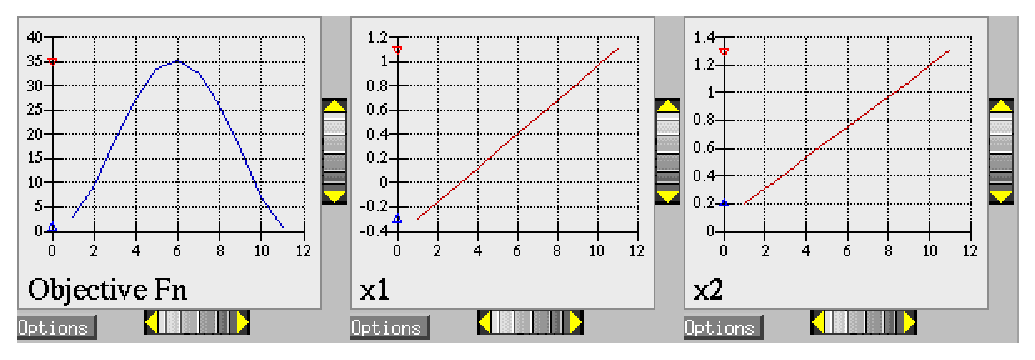
\includegraphics[width=\textwidth]{images/dak_graphics_vector}\\
  (a)\\
  \qquad\\
  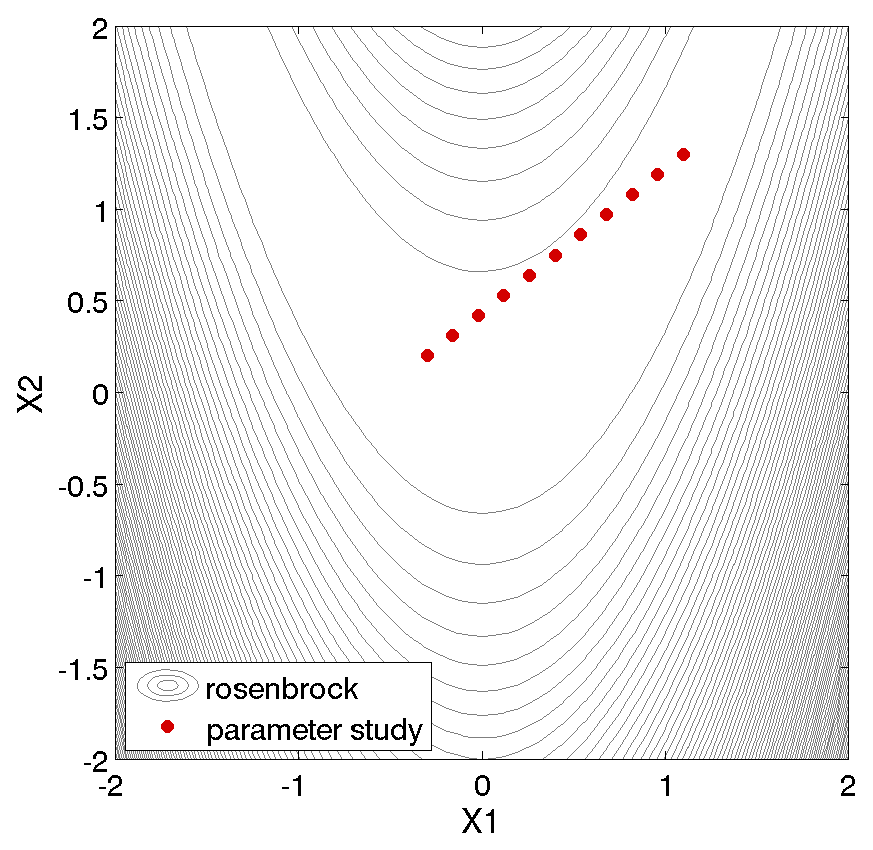
\includegraphics[height=2.5in]{images/rosen_vect_pts} \\
  (b)
  \end{tabular}
  \caption{Rosenbrock vector parameter study example: (a) screen
    capture of the DAKOTA graphics and (b) location of the design
    points (dots) evaluated.}
  \label{tutorial:rosenbrock_vector_graphics}
\end{figure}

\subsection{Optimization}\label{tutorial:example:optimization}

DAKOTA's optimization capabilities include a variety of gradient-based 
and nongradient-based optimization methods. This subsection demonstrates
the use of several such methods through the DAKOTA interface.

\subsubsection{Gradient-based Unconstrained Optimization}\label{tutorial:example:optimization:gradient1}

A DAKOTA input file for a gradient-based optimization of Rosenbrock's
function is listed in Figure~\ref{tutorial:rosenbrock_grad}. The
format of the input file is similar to that used for the parameter
studies, but there are some new keywords in the responses and method
sections.  First, in the responses section of the input file, the
keyword block starting with \texttt{numerical\_gradients} specifies
that a finite difference method will be used to compute gradients for
the optimization algorithm. Note that the Rosenbrock function
evaluation code inside DAKOTA has the ability to give analytical
gradient values.  (To switch from finite difference gradient estimates
to analytic gradients, uncomment the \texttt{analytic\_gradients}
keyword and comment out the four lines associated with the
\texttt{numerical\_gradients} specification.)
Next, in the method
section of the input file, several new keywords have been added. In
this section, the keyword \texttt{conmin\_frcg} indicates the use of
the Fletcher-Reeves conjugate gradient algorithm in the CONMIN
optimization software package~\cite{Van78} for bound-constrained
optimization.  The keyword \texttt{max\_iterations} is used to
indicate the computational budget for this optimization (in this case,
a single iteration includes multiple evaluations of Rosenbrock's
function for the gradient computation steps and the line search
steps). The keyword \texttt{convergence\_tolerance} is used to specify
one of CONMIN's convergence criteria (under which CONMIN terminates if the
objective function value differs by less than the absolute value of
the convergence tolerance for three successive iterations).
% And, finally, the \texttt{output} verbosity is set to \texttt{quiet}.

\begin{figure}
  \centering
  \begin{bigbox}
    \begin{small}
      \verbatimtabinput[8]{dakota_rosenbrock_grad_opt.in}
    \end{small}
  \end{bigbox}
  \caption{Rosenbrock gradient-based unconstrained optimization
  example: the DAKOTA input file.}
  \label{tutorial:rosenbrock_grad}
\end{figure}

This DAKOTA input file is executed using the following command:
\begin{small}
\begin{verbatim}
    dakota dakota_rosenbrock_grad_opt.in > grad_opt.out
\end{verbatim}
\end{small}

The sample file \texttt{grad\_opt.out.sav} is included in
\texttt{Dakota/examples/tutorial} for comparison. When this
example problem is executed, DAKOTA creates some iteration history
graphics similar to the screen capture shown in Figure~
\ref{tutorial:rosenbrock_grad_graphics}(a). These plots show
how the objective function and design parameters change in value
during the optimization steps. The scaling of the horizontal and
vertical axes can be changed by moving the scroll knobs on each plot.
Also, the ``Options'' button allows the user to plot the vertical axes
using a logarithmic scale.  Note that log-scaling is only allowed if
the values on the vertical axis are strictly greater than zero.

\begin{figure}[ht!]
  \centering
  \begin{tabular}{c}
  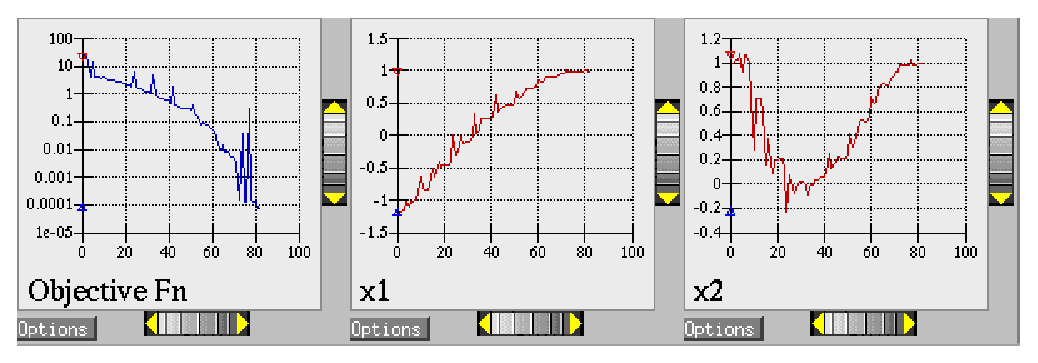
\includegraphics[width=\textwidth]{images/dak_graphics_grad_opt}\\
  (a)\\
  \qquad\\
  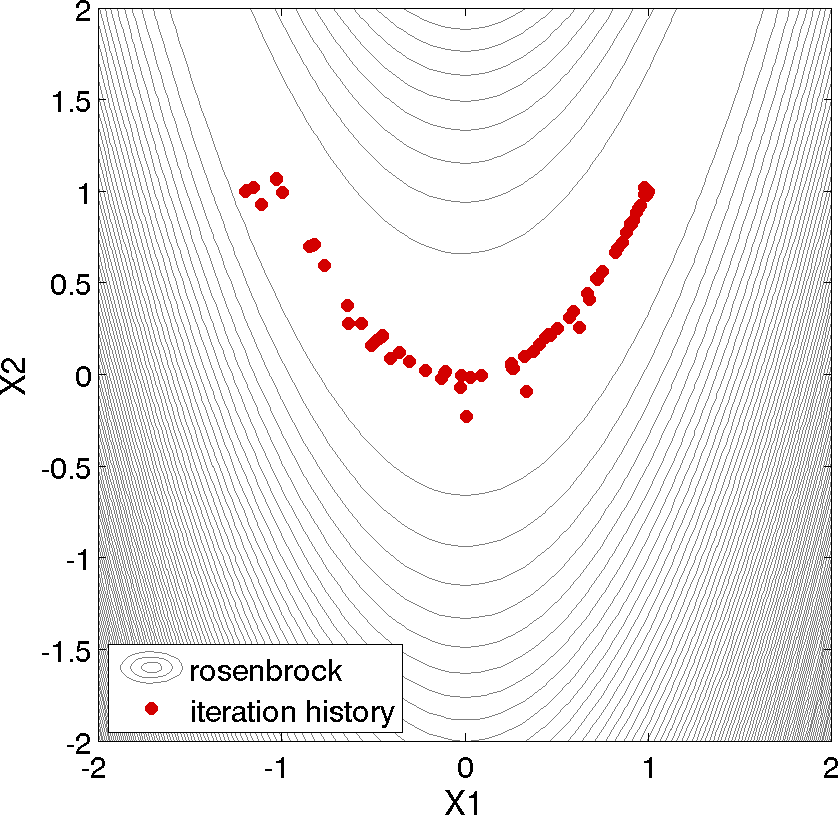
\includegraphics[height=2.5in]{images/rosen_grad_opt_pts} \\
  (b)
  \end{tabular}
  \caption{Rosenbrock gradient-based unconstrained optimization
    example: (a) screen capture of the DAKOTA graphics and (b)
    sequence of design points (dots) evaluated (line search points
    omitted).}
  \label{tutorial:rosenbrock_grad_graphics}
\end{figure}

Figure~\ref{tutorial:rosenbrock_grad_graphics}(b) shows the
iteration history of the optimization algorithm.  The optimization
starts at the point $(x_1,x_2) = (-1.2,1.0)$ as given in the
DAKOTA input file.  Subsequent iterations follow the banana-shaped
valley that curves around toward the minimum point at $(x_1,x_2) =
(1.0,1.0)$. Note that the function evaluations associated with the
line search phase of each CONMIN iteration are not shown on the plot.
At the end of the DAKOTA run, information is written to the output
file to provide data on the optimal design point. These data include
the optimum design point parameter values, the optimum objective and
constraint function values (if any), plus the number of function
evaluations that occurred and the amount of time that elapsed during
the optimization study.

\subsubsection{Gradient-based Constrained Optimization}\label{tutorial:example:gradient2}

This example demonstrates the use of a gradient-based optimization
algorithm on a nonlinearly constrained problem. The ``textbook''
example problem (see Section~\ref{tutorial:rosenbrock}) is used
for this purpose and the DAKOTA input file for this example problem is
shown in Figure~\ref{tutorial:textbook_grad_constr}.  This
input file is similar to the input file for the unconstrained
gradient-based optimization example problem involving the Rosenbrock
function.  Note the addition of commands in the responses section of
the input file that identify the number and type of constraints, along
with the upper bounds on these constraints.  The commands
\texttt{direct} and \texttt{analysis\_driver = 'text\_book'} specify
that DAKOTA will use its internal version of the textbook problem.

\begin{figure}[ht!]
  \centering
  \begin{bigbox}
    \begin{small}
      \verbatimtabinput[8]{dakota_textbook.in}
    \end{small}
  \end{bigbox}
  \caption{Textbook gradient-based constrained optimization example:
    the DAKOTA input file.}
  \label{tutorial:textbook_grad_constr}
\end{figure}

The following command runs this example problem:
\begin{small}
\begin{verbatim}
    dakota dakota_textbook.in > textbook.out
\end{verbatim}
\end{small}

The \texttt{conmin\_mfd} keyword in Figure~\ref{tutorial:textbook_grad_constr} 
tells DAKOTA to use the CONMIN package's implementation of the
Method of Feasible Directions (see Section~\ref{opt:software:conmin} 
for more details).  A significantly faster alternative is the DOT package's 
Modified Method of Feasible Directions, i.e. \texttt{dot\_mmfd} (see 
Section~\ref{opt:software:dot} for more details).  However, DOT is 
licensed software that may not be available on a particular system.  If it 
is installed on your system and DAKOTA has been compiled without the 
\texttt{--without-dot} flag, you may use it by commenting out the line with
\texttt{conmin\_mfd} and uncommenting the line with \texttt{dot\_mmfd}.

The file \texttt{textbook.out.sav} is included in
\texttt{Dakota/examples/tutorial} for comparison purposes. The
results of the optimization example problem are listed at the end of
the \texttt{textbook.out} file. This information shows that the
optimizer stopped at the point $(x_1,x_2) = (0.5,0.5)$, where both
constraints are approximately satisfied, and where the objective function value is
$0.128$. The progress of the optimization algorithm is shown in
Figure~\ref{tutorial:textbook_grad_constr_graphics}(a) where the
dots correspond to the end points of each iteration in the algorithm.  The
starting point is $(x_1,x_2) = (0.9,1.1)$, where both constraints
are violated. The optimizer takes a
sequence of steps to minimize the objective function while reducing
the infeasibility of the constraints.
The optimization graphics are also shown in
Figure~\ref{tutorial:textbook_grad_constr_graphics}(b).

\begin{figure}[ht!]
  \centering
  \begin{tabular}{c}
  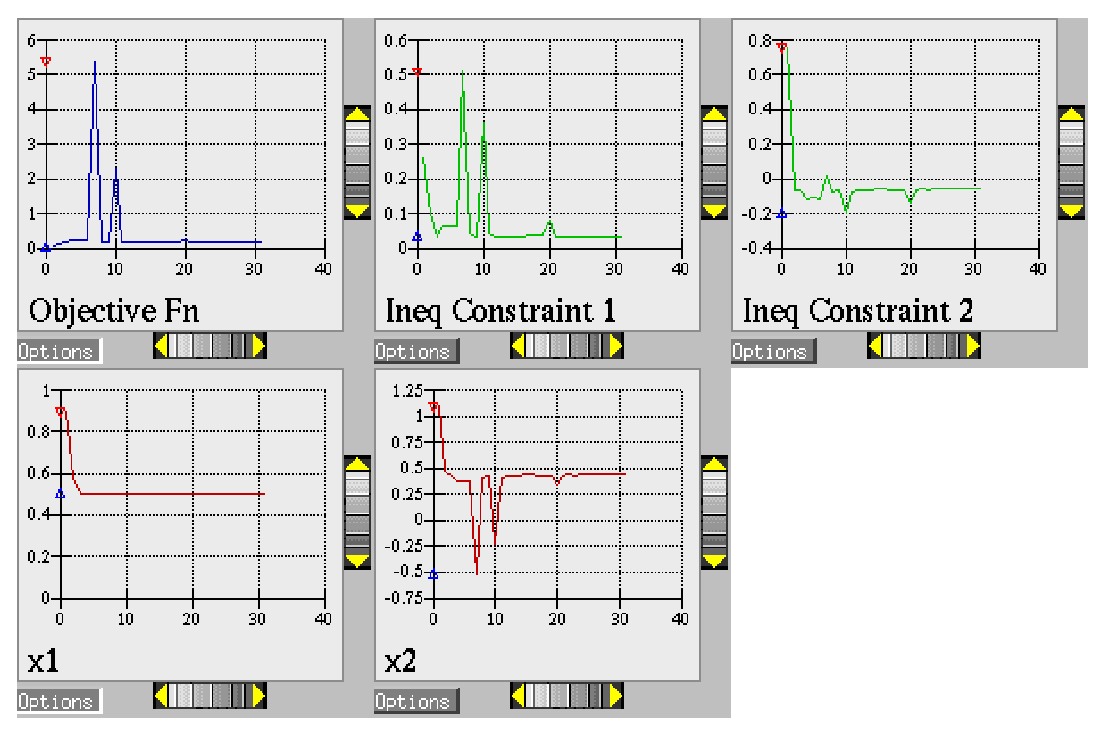
\includegraphics[width=\textwidth]{images/textbook_opt_hist}\\
  (a)\\
  \qquad\\
  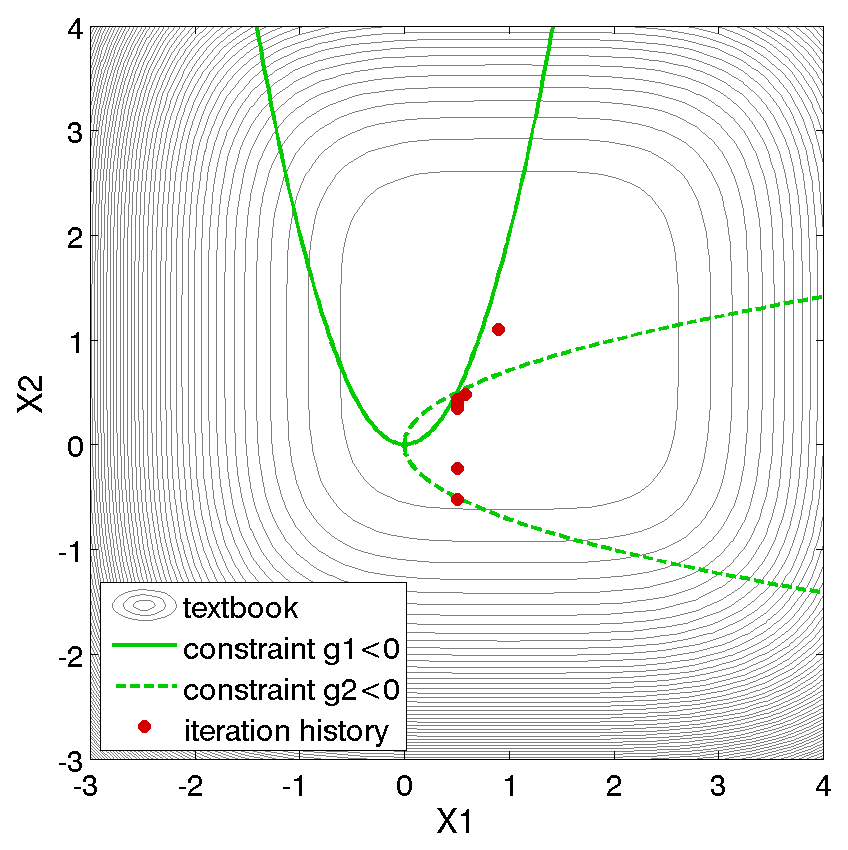
\includegraphics[height=2.5in]{images/textbook_history} \\
  (b)
  \end{tabular}
  \caption{Textbook gradient-based constrained optimization example:
    (a) screen capture of the DAKOTA graphics shows how the objective
    function was reduced during the search for a feasible design point
    and (b) iteration history (iterations marked by solid dots).}
  \label{tutorial:textbook_grad_constr_graphics}
\end{figure}

%\newpage
\subsubsection{Nonlinear Least Squares Methods for Optimization}\label{tutorial:example:nonlinear}

Both the Rosenbrock and textbook example problems can be formulated as
least-squares minimization problems (see
Section~\ref{additional:textbook} and
Section~\ref{additional:rosenbrock}). For example, the Rosenbrock
problem can be cast as:
\begin{equation}
\texttt{minimize } (f_1)^2 + (f_2)^2
\end{equation}

where $f_1 = 10(x_2-x_1^2)$ and $f_2 = (1-x_1)$. When
using a least-squares approach to minimize a function, each of the
least-squares terms $f_1, f_2,\ldots$ is driven toward zero. This
formulation permits the use of specialized algorithms that can be more
efficient than general purpose optimization algorithms. See
Chapter~\ref{nls} for more detail on the algorithms used for least-squares
minimization, as well as a discussion on the types of
engineering design problems (e.g., parameter estimation) that can make
use of the least-squares approach.

Figure~\ref{tutorial:rosenbrock_nls} is a listing of the DAKOTA input
file \texttt{dakota\_rosenbrock\_ls.in}. This input file differs from
the input file shown in Figure~\ref{tutorial:rosenbrock_grad} in
several key areas. The responses section of the input file uses the
keyword \texttt{num\_least\_squares\_terms = 2} instead of the
\texttt{num\_objective\_functions = 1}.
%The keywords in the interface section show that the Unix fork method
%is used to run the C++ analysis code named \texttt{rosenbrock}.
The method section of the input file shows that the NL2SOL
algorithm~\cite{Den81} (\texttt{nl2sol}) is used in this example.  (The
Gauss-Newton, NL2SOL, and NLSSOL SQP algorithms are currently
available for exploiting the special mathematical structure of least
squares minimization problems).

\begin{figure}[ht!]
  \centering
  \begin{bigbox}
    \begin{small}
      \verbatimtabinput[8]{dakota_rosenbrock_ls.in}
    \end{small}
  \end{bigbox}
  \caption{Rosenbrock nonlinear least squares example: the DAKOTA input file.}
  \label{tutorial:rosenbrock_nls}
\end{figure}

The input file listed in Figure~\ref{tutorial:rosenbrock_nls} is
executed using the command:
\begin{small}
\begin{verbatim}
    dakota dakota_rosenbrock_ls.in > leastsquares.out
\end{verbatim}
\end{small}

The file \texttt{leastsquares.out.sav} is included
\texttt{Dakota/examples/tutorial} for comparison purposes. The
optimization results at the end of this file show that the least
squares minimization approach has found the same optimum design point,
$(x1,x2) = (1.0,1.0)$, as was found using the conventional
gradient-based optimization approach. The iteration history of the
least squares minimization is given in
Figure~\ref{tutorial:rosenbrock_nls_graphics}, and shows that 14
function evaluations were needed for convergence. In this example the
least squares approach required about half the number of function
evaluations as did conventional gradient-based optimization.
In many cases a good least squares algorithm will converge more rapidly
in the vicinity of the solution.

\begin{figure}[ht!]
  \centering
  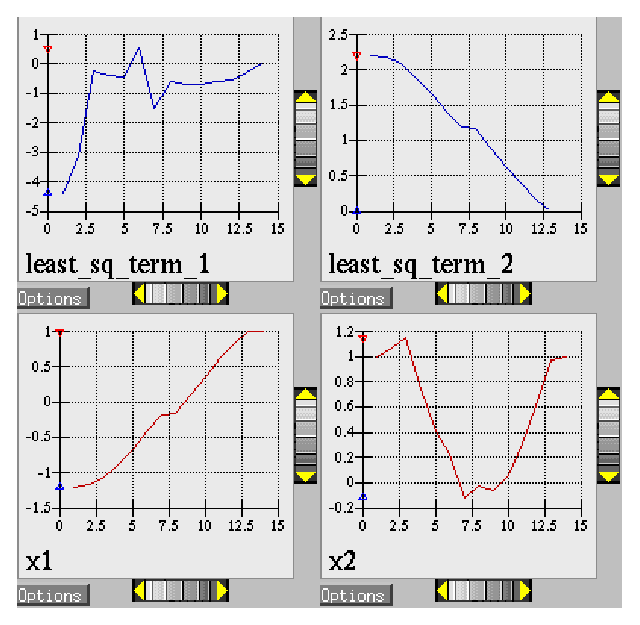
\includegraphics[height=4in]{images/nonlin_paramest_hist}
  \caption{Rosenbrock nonlinear least squares example: iteration
    history for least squares terms $f_1$ and $f_2$.}
  \label{tutorial:rosenbrock_nls_graphics}
\end{figure}

\subsubsection{Nongradient-based Optimization via Pattern Search}\label{tutorial:example:optimization:nongradient1}

In addition to gradient-based optimization algorithms, DAKOTA also
contains a variety of nongradient-based algorithms. One particular
nongradient-based algorithm for local optimization is known as pattern
search (see Chapter~\ref{introduction} for a discussion of local
versus global optimization). The DAKOTA input file shown in
Figure~\ref{tutorial:rosenbrock_patternsearch} applies a pattern
search method to minimize the Rosenbrock function.  While this
provides for an interesting comparison to the previous example
problems in this chapter, the Rosenbrock function is not the best test
case for a pattern search method. That is, pattern search methods are
better suited to problems where the gradients are too expensive to
evaluate, inaccurate, or nonexistent --- situations common among many
engineering optimization problems. It also should be noted that
nongradient-based algorithms generally are applicable only to
unconstrained or bound-constrained optimization problems, although the
inclusion of general linear and nonlinear constraints in
nongradient-based algorithms is an active area of research in the
optimization community. For most users who wish to use
nongradient-based algorithms on constrained optimization problems, the
easiest route is to create a penalty function, i.e., a composite
function that contains the objective function and the constraints,
external to DAKOTA and then optimize on this penalty function. Most
optimization textbooks will provide guidance on selecting and using
penalty functions.

The DAKOTA input file shown in
Figure~\ref{tutorial:rosenbrock_patternsearch} is similar to the
input file for the gradient-based optimization, except it has a
different set of keywords in the method section of the input file, and
the gradient specification in the responses section has been changed
to \texttt{no\_gradients}. The pattern search optimization algorithm
used is part of the SCOLIB library~\cite{Har06}.  See the DAKOTA
Reference Manual~\cite{RefMan} for more information on the
\emph{methods} section commands that can be used with SCOLIB
algorithms.

\begin{figure}[ht!]
  \centering
  \begin{bigbox}
    \begin{small}
      \verbatimtabinput[8]{dakota_rosenbrock_ps_opt.in}
    \end{small}
  \end{bigbox}
  \caption{Rosenbrock pattern search optimization example: the DAKOTA input file.}
  \label{tutorial:rosenbrock_patternsearch}
\end{figure}

This DAKOTA input file is executed using the following command:
\begin{small}
\begin{verbatim}
    dakota dakota_rosenbrock_ps_opt.in > ps_opt.out
\end{verbatim}
\end{small}

The file \texttt{ps\_opt.out.sav} is included in the
\texttt{Dakota/examples/tutorial} directory. For this run, the
optimizer was given an initial design point of $(x_1,x_2)
  = (0.0,0.0)$ and was limited to 2000 function evaluations. In this
case, the pattern search algorithm stopped short of the optimum at
$(x_1,x_2) = (1.0,1,0)$, although it was making progress
in that direction when it was terminated.  (It would have
reached the minimum point eventually.)

The iteration history is provided in Figures~
\ref{tutorial:rosenbrock_patternsearch_graphics}(a) and (b), which show
the locations of the function evaluations used in the pattern search
algorithm.
Figure~\ref{tutorial:rosenbrock_patternsearch_graphics}(c)
provides a close-up view of the pattern search function evaluations
used at the start of the algorithm. The coordinate pattern is clearly
visible at the start of the iteration history, and the decreasing size
of the coordinate pattern is evident at the design points move toward
$(x_1,x_2) = (1.0,1.0)$.

\begin{figure}[ht!]
  \centering
  \begin{tabular}{cc}
  \multicolumn{2}{c}
	      {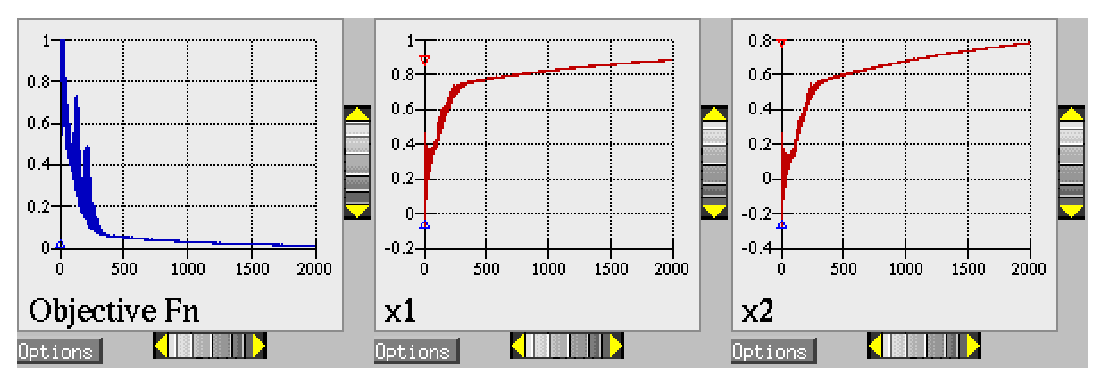
\includegraphics[width=\textwidth]{images/dak_graphics_ps_opt}}\\
  \multicolumn{2}{c}{(a)}\\
  \qquad\\
  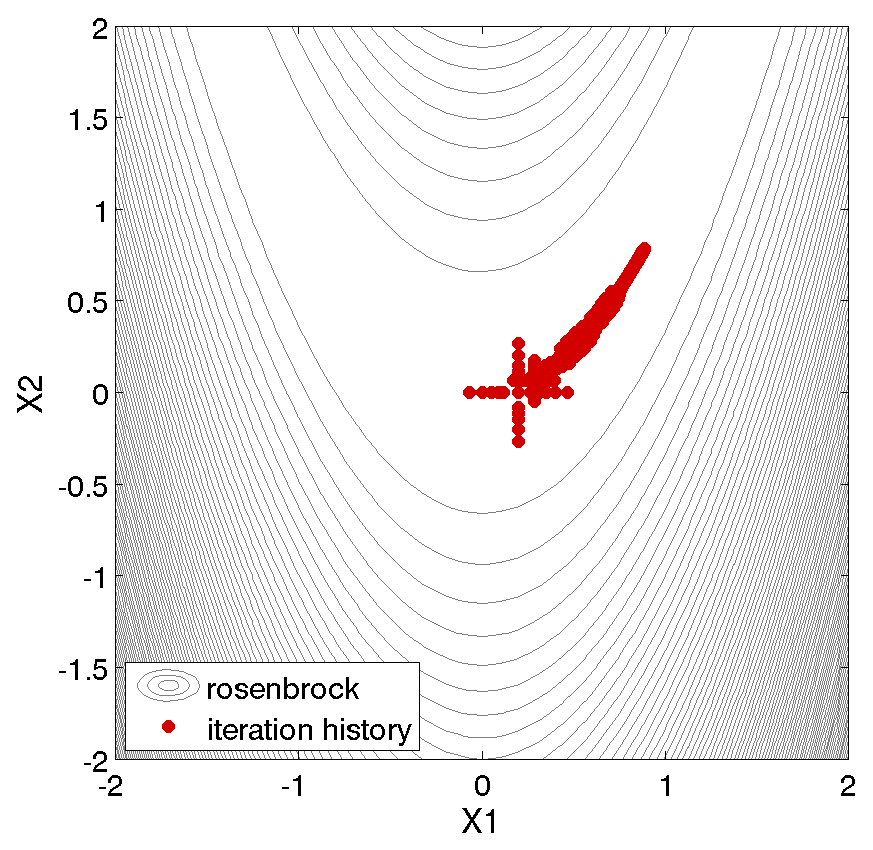
\includegraphics[height=2.5in]{images/rosen_ps_opt_pts} &
  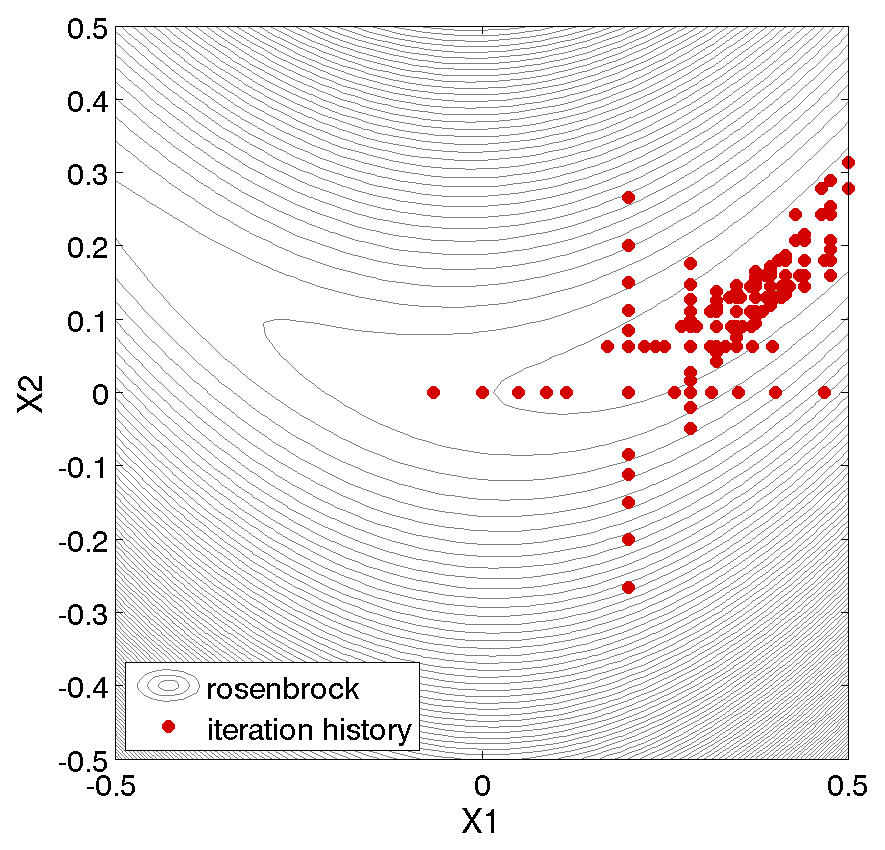
\includegraphics[height=2.5in]{images/rosen_ps_opt_pts2} \\
  (b) & (c)
  \end{tabular}
  \caption{Rosenbrock pattern search optimization example: (a) screen
    capture of the DAKOTA graphics, (b) sequence of design points
    (dots) evaluated and (c) close-up view illustrating the shape of
    the coordinate pattern used. }
  \label{tutorial:rosenbrock_patternsearch_graphics}
\end{figure}

While pattern search algorithms are useful in many optimization
problems, this example shows some of the drawbacks to this algorithm.
While a pattern search method may make good initial progress towards
an optimum, it is often slow to converge. On a smooth, differentiable
function such as Rosenbrock's function, a nongradient-based method
will not be as efficient as a gradient-based method. However, there
are many engineering design applications where gradient information is
inaccurate or unavailable, which renders gradient-based optimizers
ineffective. Thus, pattern search algorithms (and other
nongradient-based algorithms such as genetic algorithms as discussed in the
next section) are often good choices in complex engineering applications
when the quality of gradient data is suspect.

\subsubsection{Nongradient-based Optimization via Evolutionary Algorithm}\label{tutorial:example:optimization:nongradient2}

In contrast to pattern search algorithms, which are local optimization
methods, evolutionary algorithms (EA) are global optimization
methods. As was described above for the pattern search algorithm, the
Rosenbrock function is not an ideal test problem for showcasing the
capabilities of evolutionary algorithms. Rather, EAs are best suited
to optimization problems that have multiple local optima, and where
gradients are either too expensive to compute or are not readily available.

Evolutionary algorithms are based on Darwin's theory of survival of
the fittest. The EA algorithm starts with a randomly selected
population of design points in the parameter space, where the values
of the design parameters form a ``genetic string,'' analogous
to DNA in a biological system, that uniquely represents each design
point in the population. The EA then follows a sequence of
generations, where the best design points in the population (i.e.,
those having low objective function values) are considered to be the
most ``fit'' and are allowed to survive and reproduce. The EA
simulates the evolutionary process by employing the mathematical
analogs of processes such as natural selection, breeding, and
mutation. Ultimately, the EA identifies a design point (or a family of
design points) that minimizes the objective function of the
optimization problem. An extensive discussion of EAs is beyond the
scope of this text, but may be found in a variety of sources (cf.,
~\cite{Haf92} pp. 149-158;~\cite{Gol89}). Currently, the EAs available
in DAKOTA include a genetic algorithm for problems involving discrete
variables and an evolution strategy with self-adaptation for problems
with continuous variables. Details of these algorithms are given in
the DAKOTA Reference Manual~\cite{RefMan}. The SCOLIB library, which
provides the EA software that has been linked into DAKOTA, is
described in~\cite{Har06}.

\begin{figure}[ht!]
  \centering
  \begin{bigbox}
    \begin{small}
      \verbatimtabinput[8]{dakota_rosenbrock_ea_opt.in}
    \end{small}
  \end{bigbox}
  \caption{Rosenbrock evolutionary algorithm optimization example: the
  DAKOTA input file.}
  \label{tutorial:rosenbrock_ea}
\end{figure}

Figure~\ref{tutorial:rosenbrock_ea} shows a DAKOTA input file that
uses an EA to minimize the Rosenbrock function. For this
example the EA has a population size of 50. At the start of the first
generation, a random number generator is used to select 50 design
points that will comprise the initial population. \emph{[A specific
  seed value is used in this example to generate repeatable results,
  although, in general, one should use the default setting which
  allows the EA to choose a random seed.]} A two-point crossover
technique is used to exchange genetic string values between the
members of the population during the EA breeding process. The result
of the breeding process is a population comprised of the 10 best
``parent'' design points (elitist strategy) plus 40 new ``child''
design points. The EA optimization process will be terminated after
either 100 iterations (generations of the EA) or 2,000 function
evaluations. The EA software available in DAKOTA provides the user
with much flexibility in choosing the settings used in the
optimization process. See~\cite{RefMan} and~\cite{Har06} for details on these
settings.

The following command runs DAKOTA on the input file:
\begin{small}
\begin{verbatim}
    dakota dakota_rosenbrock_ea_opt.in > ea_opt.out
\end{verbatim}
\end{small}

A corresponding output file named \texttt{ea\_opt.out.sav} appears in
\texttt{Dakota/examples/tutorial}. The EA optimization results
printed at the end of this file show that the best design point found
was $(x_1,x_2) = (0.98,0.95)$. The file
\texttt{ea\_tabular.dat.sav} provides a listing of the design
parameter values and objective function values for all 2,000 design
points evaluated during the running of the EA.  Figure~
\ref{tutorial:rosenbrock_ea_graphics}(a) shows the population of
50 randomly selected design points that comprise the first generation
of the EA, and Figure~\ref{tutorial:rosenbrock_ea_graphics}(b)
shows the final population of 50 design points, where most of the 50
points are clustered near $(x_1,x_2) = (0.98,0.95)$.

\begin{figure}[hbt!]
  \centering
  \begin{tabular}{cc}
  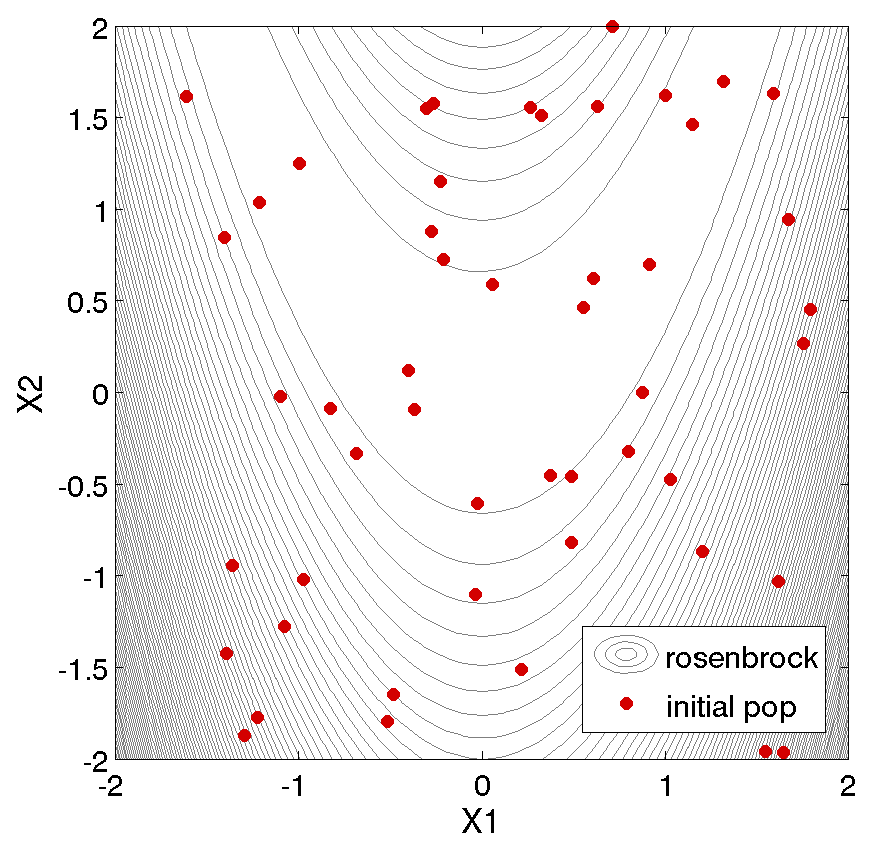
\includegraphics[height=2.5in]{images/rosen_ea_init} &
  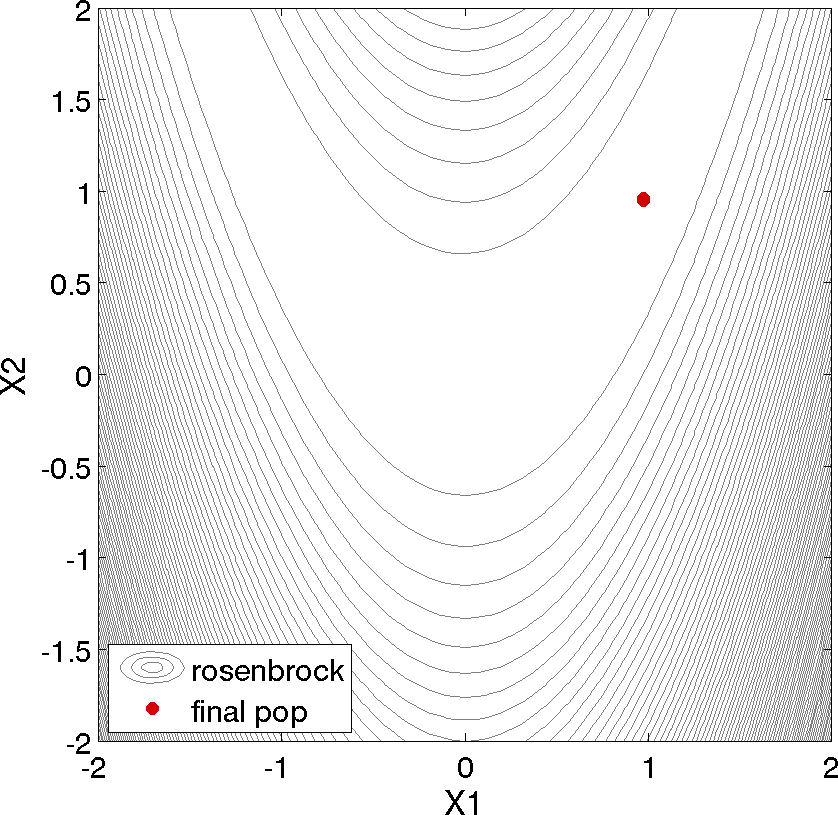
\includegraphics[height=2.5in]{images/rosen_ea_final} \\
  (a) & (b)
  \end{tabular}
  \caption{Rosenbrock evolutionary algorithm optimization example: 50
    design points in the (a) initial and (b) final populations
    selected by the evolutionary algorithm. }
  \label{tutorial:rosenbrock_ea_graphics}
\end{figure}

As described above, an EA is not well-suited to an optimization
problem involving a smooth, differentiable objective such as the
Rosenbrock function. Rather, EAs are better suited to optimization
problems where conventional gradient-based optimization fails, such as
situations where there are multiple local optima and/or gradients are
not available. In such cases, the computational expense of an EA is
warranted since other optimization methods are not applicable or
impractical. In many optimization problems, EAs often quickly identify
promising regions of the design space where the global minimum may be
located. However, an EA can be slow to converge to the optimum. For
this reason, it can be an effective approach to combine the global
search capabilities of a EA with the efficient local search of a
gradient-based algorithm in a \emph{hybrid optimization} strategy.  In
this approach, the optimization starts by using a few iterations of a
EA to provide the initial search for a good region of the parameter
space (low objective function and/or feasible constraints), and then
it switches to a gradient-based algorithm (using the best design point
found by the EA as its starting point) to perform an efficient local
search for an optimum design point. More information on this hybrid
approach is provided in Chapter~\ref{strat}.

In addition to the evolutionary algorithm capabilities in the
\texttt{coliny\_ea} method, there is a single-objective genetic algorithm
method called \texttt{soga}.
%The major differences are that
%\texttt{soga} allows a warm start (e.g., you can read in starting
%solutions from a file), and it allows one to specify a mix of
%continuous and discrete design variables.
For more information on \texttt{soga}, see Chapter~\ref{opt}.

\subsubsection{Multiobjective Optimization}\label{tutorial:example:optimization:multiobjective}

Multiobjective optimization means that there are two or more
objective functions that you wish to optimize simultaneously.  Often
these are conflicting objectives, such as cost and performance.  The
answer to a multi-objective problem is usually not a single point.
Rather, it is a set of points called the Pareto front.  Each point
on the Pareto front satisfies the Pareto optimality criterion, i.e.,
locally there exists no other feasible vector that would improve some
objective without causing a simultaneous worsening in at least one
other objective.  Thus a feasible point $X^\prime$ from which
small moves improve one or more objectives without worsening
any others is not Pareto optimal: it is said to be ``dominated''
and the points along the Pareto front are said to be
``non-dominated''.

Often multi-objective problems are addressed by simply assigning
weights to the individual objectives, summing the weighted
objectives, and turning the problem into a single-objective one
which can be solved with a variety of optimization techniques. While
this approach provides a useful ``first cut'' analysis (and is
supported within DAKOTA---see Section~\ref{opt:additional}), this
approach has many limitations.  The major limitation is that a
local solver with a weighted sum objective will only find one
% optimal solutions if the true Pareto front is nonconvex. %Hogwash!
point on the Pareto front; if one wants to understand
the effects of changing weights, this method can be computationally
expensive.  Since each optimization of a single weighted objective
will find only one point on the Pareto front, many
optimizations must be performed to get a good parametric
understanding of the influence of the weights and to achieve a good
sampling of the entire Pareto frontier.

Starting with version 3.2 of DAKOTA, a capability to perform
multi-objective optimization based on a genetic algorithm method has
been available.  This method is called \texttt{moga}.  It is based on
the idea that as the population evolves in a GA, solutions that are
non-dominated are chosen to remain in the population.  Until version
4.0 of DAKOTA, there was a selection\_type choice of domination\_count
that performed a custom fitness assessment and selection operation
together.  As of version 4.0 of DAKOTA, that functionality has been
broken into separate, more generally usable fitness assessment and
selection operators called the domination\_count fitness assessor and
below\_limit selector respectively.  The effect of using these two
operators is the same as the previous behavior of the
domination\_count selector.  This means of selection works especially
well on multi-objective problems because it has been specifically
designed to avoid problems with aggregating and scaling objective
function values and transforming them into a single
objective. Instead, the fitness assessor works by ranking population
members such that their resulting fitness is a function of the number
of other designs that dominate them.  The below\_limit selector then
chooses designs by considering the fitness of each. If the fitness of
a design is above a certain limit, which in this case corresponds to a
design being dominated by more than a specified number of other
designs, then it is discarded. Otherwise it is kept and selected to go
to the next generation. The one catch is that this selector will
require that a minimum number of selections take
place. The \texttt{shrinkage\_percentage} determines the minimum number of
selections that will take place if enough designs are available. It is
interpreted as a percentage of the population size that must go on to
the subsequent generation. To enforce this, the below\_limit selector
makes all the selections it would make anyway and if that is not
enough, it relaxes its limit and makes selections from the remaining
designs.  It continues to do this until it has made enough selections.
The moga method has many other important features.  Complete
descriptions can be found in the DAKOTA Reference Manual~\cite{RefMan}.

Figure~\ref{tutorial:moga} shows an example input file that
demonstrates some of the multi-objective capabilities available with
the moga method.
\begin{figure}[htp!]
  \centering
  \begin{bigbox}
    \begin{small}
      \verbatimtabinput[8]{dakota_mogatest1.in}
    \end{small}
  \end{bigbox}
  \caption{Multiple objective genetic algorithm (MOGA) example: the
    DAKOTA input file.}
  \label{tutorial:moga}
\end{figure}

This example has three input variables and two objectives.
The example uses objectives different from the Rosenbrock
function because we wanted to demonstrate the capability on a problem
with two conflicting objectives.  This example is taken from a testbed
of multi-objective problems~\cite{Coe02}. In this example, the three best solutions (as specified by \texttt{final\_solutions} =3) are written to the output.  Additionally, final results from moga
are output to a file called \texttt{finaldata1.dat} in the directory in
which you are running. This \texttt{finaldata1.dat} file is simply a
list of inputs and outputs. Plotting the output columns against each
other allows one to see the Pareto front generated by \texttt{moga}.
Figure~\ref{tutorial:moga_pareto} shows an example of the Pareto
front for this problem. Note that a Pareto front easily shows the
tradeoffs between Pareto optimal solutions.  For example, look at the
point with f1 and f2 values equal to (0.9, 0.23). One cannot improve
(minimize) the value of objective function f1 without increasing the
value of f2: another point on the Pareto front, (0.63, 0.63) represents
a better value of objective f1 but a worse value of objective f2.
\begin{figure}[ht!]
  \centering
  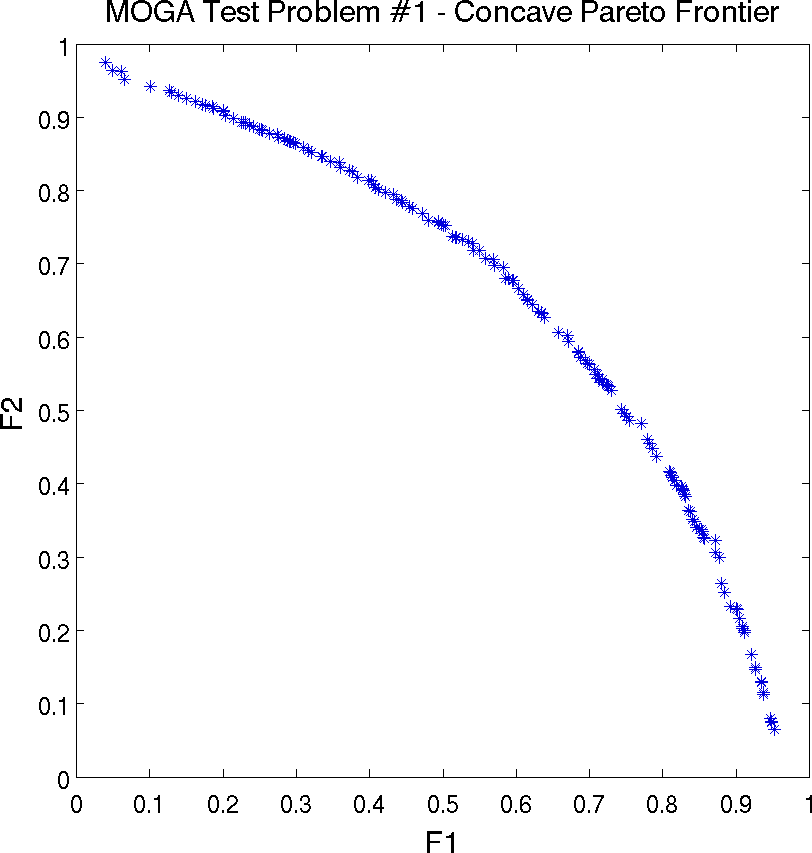
\includegraphics[scale=0.75]{images/dakota_mogatest1_pareto_front}
  \caption{Multiple objective genetic algorithm (MOGA) example: Pareto
  front showing tradeoffs between functions f1 and f2.}
  \label{tutorial:moga_pareto}
\end{figure}

Sections~\ref{opt:software} and~\ref{opt:additional} provide more
information on multiobjective optimization.  There are three detailed
examples provided in Section~\ref{additional:multiobjective}.

\subsection{Uncertainty Quantification}\label{tutorial:example:uncert_quant}

Uncertainty quantification (UQ) is the process of determining the
effect of input uncertainties on response metrics of interest.  These
input uncertainties may be characterized as either aleatory
uncertainties, which are irreducible variabilities inherent in nature,
or epistemic uncertainties, which are reducible uncertainties
resulting from a lack of knowledge.  Since sufficient data is
generally available for aleatory uncertainties, probabilistic methods
are commonly used for computing response distribution statistics based
on input probability distribution specifications.  Conversely, for
epistemic uncertainties, data is generally sparse, making the use of
probability theory questionable and leading to nonprobabilistic
methods based on interval specifications.

The subsection demonstrates the use of several methods of uncertainty 
quantification methods built into DAKOTA.  These examples include 
Monte Carlo random sampling, reliability methods, the representation 
of a stochastic process by a polynomial chaos expansion, 
and interval analysis.  

\subsubsection{Monte Carlo Sampling}\label{tutorial:example:uncert_quant:monte_carlo}

Figure~\ref{tutorial:rosenbrock_mc} shows the DAKOTA input file for
an example problem that demonstrates some of the random sampling
capabilities available in DAKOTA. In this example, the design
parameters, x1 and x2, will be treated as uncertain parameters that
have uniform distributions over the interval [-2, 2]. This is
specified in the variables section of the input file, beginning with
the keyword \texttt{uniform\_uncertain}.
% Not true: For comparison, the keywords
% from the previous examples are retained, but have been commented out.
Another change from earlier input files, such as
Figure~\ref{tutorial:rosenbrock_vector},
occurs in the responses section, where
the keyword \texttt{num\_response\_functions} is used in place of
\texttt{num\_objective\_functions}. The final changes to the input
file occur in the method section, where the keyword
\texttt{sampling} is used; ``nond'' is an abbreviation for 
nondeterministic.
The other keywords in the methods section of the input file
specify the number of samples (200), the seed for the random number
generator (17), the sampling method (random), and the response
threshold (100.0). The \texttt{seed} specification allows a user to
obtain repeatable results from multiple runs. If a seed value is not
specified, then DAKOTA's sampling methods are designed to generate
nonrepeatable behavior (by initializing the seed using a system
clock). The keyword \texttt{response\_thresholds} allows the user to
specify threshold values for which DAKOTA will compute statistics on
the response function output.  Note that a unique threshold value can
be specified for each response function.

In this example, DAKOTA will select 200 design points from within the
parameter space, evaluate the value of Rosenbrock's function at all
200 points, and then perform some basic statistical calculations on
the 200 response values.

This DAKOTA input file is executed using the following command:
\begin{small}
\begin{verbatim}
         dakota dakota_rosenbrock_nond.in > nond.out
\end{verbatim}
\end{small}

Figure~\ref{tutorial:results_mc} shows example results from this 
sampling method.  See the \texttt{nond.out.sav} file in directory
\texttt{Dakota/examples/tutorial} for comparison with results
produced by DAKOTA. Note that your results will differ from those in
this file if your \texttt{seed} value differs or if no \texttt{seed}
is specified.


As shown in Figure~\ref{tutorial:results_mc}, 
the statistical data on the 200 Monte Carlo samples is printed at the
end of the output file in the section that starts with ``Statistics
based on 200 samples.'' In this section summarizing 
moment-based statistics, DAKOTA outputs the
mean, standard deviation, skewness, and kurtosis estimates 
for each of the response functions.  For example, 
the mean of the Rosenbrock function given uniform input uncertainties 
on the input variables is 455.4 and the standard deviation is 536.8. 
This is a very large standard deviation, due to the fact that the 
Rosenbrock function varies by three orders of magnitude over the input 
domain.  The skewness is positive, meaning this is a right-tailed distribution, not a symmetric distribution.  Finally, the kurtosis (a measure of the ``peakedness'' of the distribution) indicates that 
this is a strongly peaked distribution (note that we use a central, standardized kurtosis so that the kurtosis of a normal is zero).  After the moment-related statistics, the 95\% confidence intervals on the mean and standard deviations are printed.  This is followed by
the fractions (``Probability Level'') of the response function values 
that are below the response threshold values specified in the input file. 
For example, 34 percent of the sample inputs resulted in a Rosenbrock 
function value that was less than or equal to 100, as shown in the line 
listing the cumulative distribution function values.  
Finally, there are several 
correlation matrices printed at the end, showing simple and partial 
raw and rank correlation matrices.  Correlations provide an indication 
of the strength of a monotonic relationship between input and outputs.  
More detail on correlation coefficients and their interpretation can be 
found in Section~\ref{uq:uncertainty1}. 
More detail about sampling methods in general can be found in 
Section~\ref{uq:sampling}.  Finally,  
Figure~\ref{tutorial:rosenbrock_mc_points} shows the locations
of the 200 sample sites within the parameter space of the Rosenbrock
function for this example.

\begin{figure}[ht!]
  \centering
  \begin{bigbox}
    \begin{small}
      \verbatimtabinput[8]{dakota_rosenbrock_nond.in}
    \end{small}
  \end{bigbox}
  \caption{Monte Carlo sampling example: the DAKOTA input file.}
  \label{tutorial:rosenbrock_mc}
\end{figure}

\begin{figure}
\centering
\begin{bigbox}
\begin{footnotesize}
\begin{verbatim}
Statistics based on 200 samples:

Moment-based statistics for each response function:
                            Mean           Std Dev          Skewness          Kurtosis
 response_fn_1  4.5540183516e+02  5.3682678089e+02  1.6661798252e+00  2.7925726822e+00

95% confidence intervals for each response function:
                    LowerCI_Mean      UpperCI_Mean    LowerCI_StdDev    UpperCI_StdDev
 response_fn_1  3.8054757609e+02  5.3025609422e+02  4.8886795789e+02  5.9530059589e+02

Level mappings for each response function:
Cumulative Distribution Function (CDF) for response_fn_1:
     Response Level  Probability Level  Reliability Index  General Rel Index
     --------------  -----------------  -----------------  -----------------
   1.0000000000e+02   3.4000000000e-01

Probability Density Function (PDF) histograms for each response function:
PDF for response_fn_1:
          Bin Lower          Bin Upper      Density Value
          ---------          ---------      -------------
   1.1623549854e-01   1.0000000000e+02   3.4039566059e-03
   1.0000000000e+02   2.7101710856e+03   2.5285698843e-04

Simple Correlation Matrix among all inputs and outputs:
                       x1           x2 response_fn_1 
          x1  1.00000e+00 
          x2 -5.85097e-03  1.00000e+00 
response_fn_1 -9.57746e-02 -5.08193e-01  1.00000e+00 

Partial Correlation Matrix between input and output:
             response_fn_1 
          x1 -1.14659e-01 
          x2 -5.11111e-01 

Simple Rank Correlation Matrix among all inputs and outputs:
                       x1           x2 response_fn_1 
          x1  1.00000e+00 
          x2 -6.03315e-03  1.00000e+00 
response_fn_1 -1.15360e-01 -5.04661e-01  1.00000e+00 

Partial Rank Correlation Matrix between input and output:
             response_fn_1 
          x1 -1.37154e-01 
          x2 -5.08762e-01 
\end{verbatim}
\end{footnotesize}
\end{bigbox}
\caption{Results of Monte Carlo Sampling on the Rosenbrock Function}
\label{tutorial:results_mc}
\end{figure}


\begin{figure}[ht!]
  \centering
  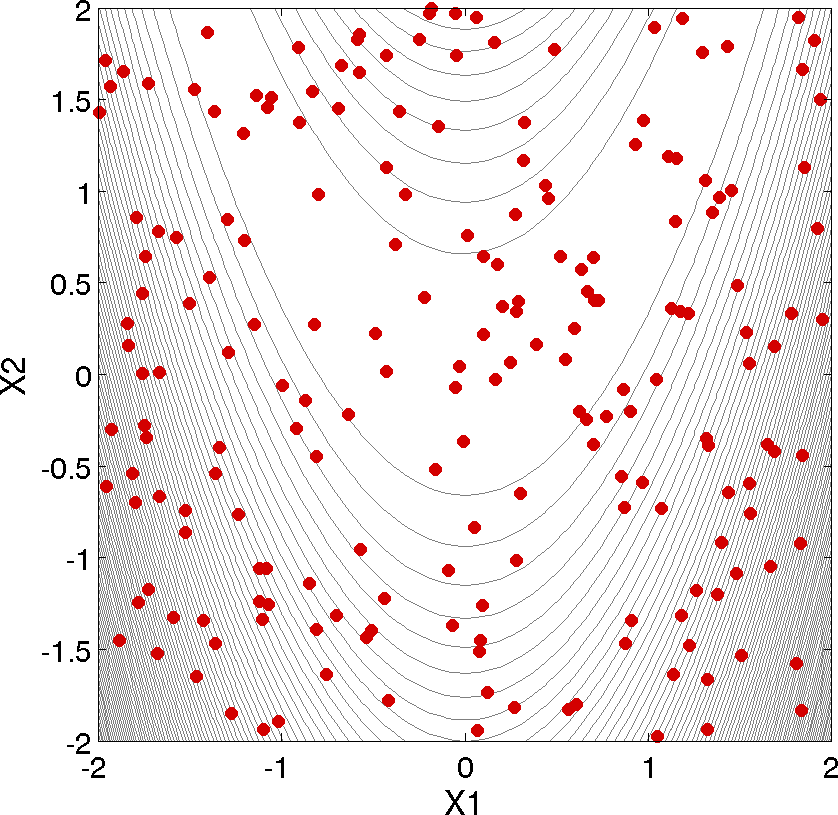
\includegraphics[height=2.5in]{images/rosen_nond_pts}
  \caption{Monte Carlo sampling example: locations in the parameter
    space of the 200 Monte Carlo samples using a uniform distribution
    for both $x_1$ and $x_2$.}
  \label{tutorial:rosenbrock_mc_points}
\end{figure}

%\newpage

\subsubsection{Reliability Methods - via the Mean Value Method}\label{tutorial:example:uncert_quant:reliability}

Reliability methods provide an alternative approach to uncertainty
quantification which can be less computationally demanding than
sampling techniques.  Reliability methods for uncertainty
quantification are based on probabilistic approaches that compute
approximate response function distribution statistics based on
specified uncertain variable distributions.  These response statistics
include response mean, response standard deviation, and cumulative or
complementary cumulative distribution functions (CDF/CCDF).  These
methods are often more efficient at computing statistics in the tails
of the response distributions (events with low probability) than
sampling based approaches since the number of samples required to
resolve a low probability can be prohibitive.

Figure~\ref{tutorial:textbook_mv} shows the DAKOTA input file for an
example problem that demonstrates the simplest reliability method,
called the mean value method (also referred to as the Mean Value First
Order Second Moment method).  It is specified with method keyword
\texttt{local\_reliability}.  This method calculates the mean and
variance of the response function based on information about the mean
and variance of the inputs and gradient information at the mean of the
inputs. The mean value method is extremely cheap computationally (only
five runs were required for the textbook function), but can be quite
inaccurate, especially for nonlinear problems and/or problems with
uncertain inputs that are significantly non-normal. More detail on the
mean value method can be found in the Local Reliability Methods
section of the DAKOTA Theory Manual~\cite{TheoMan}, and more detail on
reliability methods in general (including the more advanced methods)
is found in Section~\ref{uq:reliability}.

Example output from the mean value method is displayed in 
Figure~\ref{tutorial:results_mv}. Note that since the mean of both inputs
is 1, the mean value of the output for response 1 is zero. 
However, the mean values of the constraints are both 0.5. 
The mean value results indicate that variable x1 is more 
important in constraint 1 while x2 is more important in constraint 2, 
which is the case based on Equation~\ref{tutorial:textbook_f}.

This DAKOTA input file is executed using the following command:
\begin{small}
\begin{verbatim}
         dakota dakota_mv.in > mv.out
\end{verbatim}
\end{small}
See the file \texttt{mv.out.sav} in \texttt{Dakota/examples/tutorial} 
for comparison with results from DAKOTA. 

\begin{figure}[ht!]
  \centering
  \begin{bigbox}
    \begin{small}
      \verbatimtabinput[8]{dakota_mv.in}
    \end{small}
  \end{bigbox}
  \caption{Mean Value Reliability Method: the DAKOTA input file.}
  \label{tutorial:textbook_mv}
\end{figure}

\begin{figure}
\centering
\begin{bigbox}
\begin{small}
\begin{verbatim}
-----------------------------------------------------------------
MV Statistics for response_fn_1:
  Approximate Mean Response                  =  0.0000000000e+00
  Approximate Standard Deviation of Response =  0.0000000000e+00
  Importance Factors not available.
MV Statistics for response_fn_2:
  Approximate Mean Response                  =  5.0000000000e-01
  Approximate Standard Deviation of Response =  1.0307764064e+00
  Importance Factor for variable TF1ln       =  9.4117647059e-01
  Importance Factor for variable TF2ln       =  5.8823529412e-02
MV Statistics for response_fn_3:
  Approximate Mean Response                  =  5.0000000000e-01
  Approximate Standard Deviation of Response =  1.0307764064e+00
  Importance Factor for variable TF1ln       =  5.8823529412e-02
  Importance Factor for variable TF2ln       =  9.4117647059e-01
-----------------------------------------------------------------
\end{verbatim}
\end{small}
\end{bigbox}
\caption{Results of the Mean Value Method on the Textbook Function}
\label{tutorial:results_mv}
\end{figure}


\subsubsection{Polynomial Chaos}\label{tutorial:example:uncert_quant:poly_chaos}
The term ``Polynomial Chaos'' refers to the representation of a stochastic 
process as a polynomial expansion in random (or stochastic) variables. This 
representation acts as a response surface that maps stochastic inputs to 
stochastic outputs.  Desired statistics can then be obtained from the 
response surface either analytically or by re-sampling the fast surrogate.
Exponential convergence of the error with increasing polynomial order can 
be obtained by using (an) orthogonal polynomial series whose weighting 
function(s) is/are the probability density functions of the stochastic 
inputs. Coefficients in the Chaos expansion are determined through
orthogonal projection. For non-intrusive implementations, such as in DAKOTA,
numerical integration via quadrature or cubature is used to evaluate the 
orthogonal projections.  Additional details regarding the method are 
provided in Section~\ref{uq:expansion}.

A typical DAKOTA input file for performing an uncertainty
quantification using polynomial chaos expansions is shown in
Figure~\ref{tutorial:pce}, \texttt{dakota\_pce.in}.
In this example, we compute CDF
probabilities for six response levels of Rosenbrock's function.  Since
Rosenbrock is a fourth order polynomial and we employ a fourth-order
expansion using an optimal basis (Legendre for uniform random
variables), we can readily obtain a polynomial expansion which exactly
matches the Rosenbrock function.  In this example, we select Gaussian
quadratures using an anisotropic approach (fifth-order quadrature in
$x_1$ and third-order quadrature in $x_2$), resulting in a total of
15 function evaluations to compute the PCE coefficients.

\begin{figure}
  \centering
  \begin{bigbox}
    \begin{small}
      \verbatimtabinput[8]{dakota_pce.in}
    \end{small}
  \end{bigbox}
\caption{DAKOTA input file for performing UQ using polynomial chaos expansions.}
\label{tutorial:pce}
\end{figure}

The tensor product quadature points upon which the expansion is calculated 
are shown in Figure~\ref{tutorial:rosen_pce_points}.  
The tensor product generates
all combinations of values from each individual dimension: it is an 
all-way pairing of points.

\begin{figure}[ht!]
  \centering
  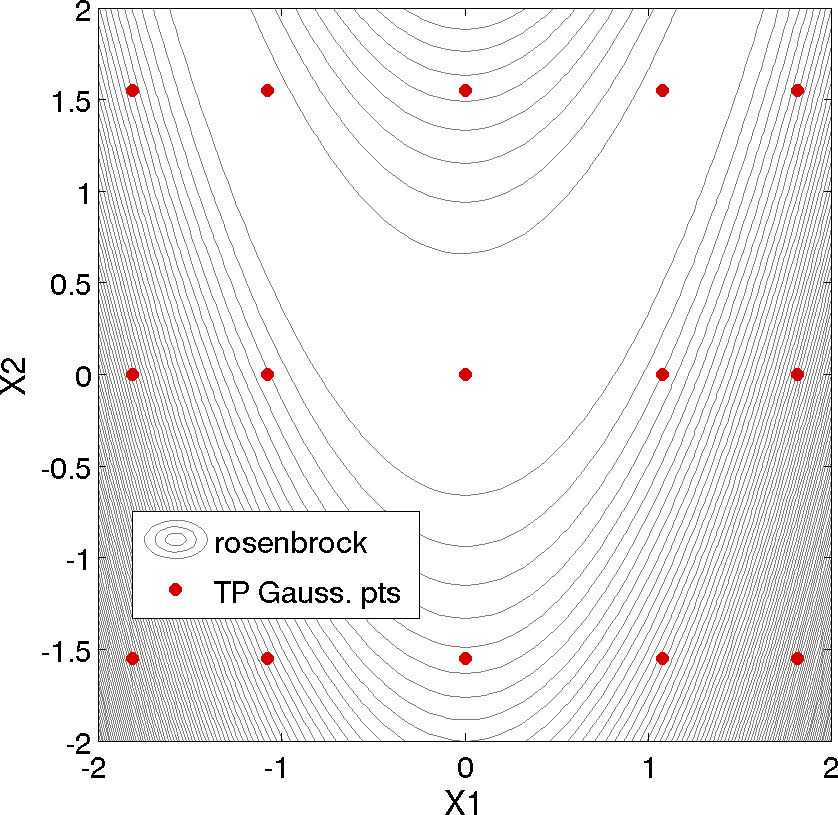
\includegraphics[height=2.5in]{images/rosen_pce_pts}
  \caption{Rosenbrock polynomial chaos example: tensor product quadrature points.}
  \label{tutorial:rosen_pce_points}
\end{figure}

Once the expansion coefficients have been calculated, some statistics
are available analytically and others must be evaluated numerically.
For the numerical portion, the input file specifies the use of 10000
samples, which will be evaluated on the expansion to compute the CDF
probabilities.  In Figure~\ref{tutorial:pce_out}, excerpts from the results
summary are presented, where we first see a summary of the PCE
coefficients which exactly reproduce Rosenbrock for a Legendre
polynomial basis.  The analytic statistics for mean, standard
deviation, and COV are then presented.  For example, the mean is 455.66 
and the standard deviation is 606.56.  The moments are followed 
by global sensitivity indices (Sobol indices).This example shows that variable 
x1 has the largest main effect (0.497) as compared with variable 
x2 (0.296) or the interaction between x1 and x2 (0.206). 
After the global sensitivity indices, the local, analytic random 
variable sensitivities are presented, evaluated at the mean values.
Finally, we see the numerical results for the CDF probabilities based
on 10000 samples performed on the expansion. For example, 
the probability that the Rosenbrock function is less than 100 
over these two uncertain variables is 0.342. Note that this is a very similar 
estimate to what was obtained using 200 Monte Carlo samples, with 
fewer function evaluations.
\begin{figure}
\centering
\begin{bigbox}
%\begin{footnotesize}
\begin{scriptsize}
\begin{verbatim}
Polynomial Chaos coefficients for response_fn_1:
        coefficient   u1   u2
        ----------- ---- ----
   4.5566666667e+02   P0   P0
  -4.0000000000e+00   P1   P0
   9.1695238095e+02   P2   P0
  -9.9475983006e-14   P3   P0
   3.6571428571e+02   P4   P0
  -5.3333333333e+02   P0   P1
  -3.9968028887e-14   P1   P1
  -1.0666666667e+03   P2   P1
  -3.3573144265e-13   P3   P1
   1.2829737273e-12   P4   P1
   2.6666666667e+02   P0   P2
   2.2648549702e-13   P1   P2
   4.8849813084e-13   P2   P2
   2.8754776338e-13   P3   P2
  -2.8477220582e-13   P4   P2
-------------------------------------------------------------------
Statistics derived analytically from polynomial expansion:

Moment-based statistics for each response function:
                            Mean           Std Dev          Skewness          Kurtosis
response_fn_1
  expansion:    4.5566666667e+02  6.0656024184e+02
  numerical:    4.5566666667e+02  6.0656024184e+02  1.9633285271e+00  3.3633861456e+00

Covariance among response functions:
[[  3.6791532698e+05 ]] 

Local sensitivities for each response function evaluated at uncertain variable means:
response_fn_1:
 [ -2.0000000000e+00  2.4055757386e-13 ] 

Global sensitivity indices for each response function:
response_fn_1 Sobol indices:
                                  Main             Total
                      4.9746891383e-01  7.0363551328e-01 x1
                      2.9636448672e-01  5.0253108617e-01 x2
                           Interaction
                      2.0616659946e-01 x1 x2 

Statistics based on 10000 samples performed on polynomial expansion:

Probability Density Function (PDF) histograms for each response function:
PDF for response_fn_1:
          Bin Lower          Bin Upper      Density Value
          ---------          ---------      -------------
   6.8311107124e-03   1.0000000000e-01   2.0393073423e-02
   1.0000000000e-01   1.0000000000e+00   1.3000000000e-02
   1.0000000000e+00   5.0000000000e+01   4.7000000000e-03
   5.0000000000e+01   1.0000000000e+02   1.9680000000e-03
   1.0000000000e+02   5.0000000000e+02   9.2150000000e-04
   5.0000000000e+02   1.0000000000e+03   2.8300000000e-04
   1.0000000000e+03   3.5755437782e+03   5.7308286215e-05

Level mappings for each response function:
Cumulative Distribution Function (CDF) for response_fn_1:
     Response Level  Probability Level  Reliability Index  General Rel Index
     --------------  -----------------  -----------------  -----------------
   1.0000000000e-01   1.9000000000e-03
   1.0000000000e+00   1.3600000000e-02
   5.0000000000e+01   2.4390000000e-01
   1.0000000000e+02   3.4230000000e-01
   5.0000000000e+02   7.1090000000e-01
   1.0000000000e+03   8.5240000000e-01
-------------------------------------------------------------------
\end{verbatim}
\end{scriptsize}
%\end{footnotesize}
\end{bigbox}
\caption{Excerpt of UQ output for polynomial chaos example.}
\label{tutorial:pce_out}
\end{figure}

\subsubsection{Interval Analysis}\label{tutorial:example:uncert_quant:interval}

Interval analysis is often used to model epistemic uncertainty. 
In interval analysis, one assumes that nothing is known about 
an epistemic uncertain variable except that its value lies 
somewhere within an interval.  In this situation, it is NOT 
assumed that the value has a uniform probability of occuring 
within the interval.  Instead, the interpretation is that 
any value within the interval is a possible value or a potential 
realization of that variable.  In interval analysis, the 
uncertainty quantification problem is one of determining the 
resulting bounds on the output (defining the output interval) 
given interval bounds on the inputs. Again, any output response 
that falls within the output interval is a possible output 
with no frequency information assigned to it.

We can do interval analysis using either
\texttt{global\_interval\_est} or \texttt{local\_interval\_est}.
In the global approach, one uses either a global optimization 
method or a sampling method to assess the bounds, whereas the 
local method uses gradient information in a derivative-based 
optimization approach. 
 
An example of interval estimation 
is found in the test file \texttt{dakota\_uq\_interval.in}, 
and also in Figure~\ref{tutorial:interval}, with example results in 
Figure~\ref{tutorial:interval_out}. This example is a demonstration 
of calculating interval bounds for three outputs of the cantilever beam 
problem. The cantilever beam problem is described in detail in 
Section~\ref{additional:cantilever}. Given input intervals of [1,10] on 
beam width and beam thickness, we can see that the interval estimate of 
beam weight is approximately [1,100].

\begin{figure}
  \centering
  \begin{bigbox}
    \begin{small}
      \verbatimtabinput[8]{dakota_uq_interval.in}
    \end{small}
  \end{bigbox}
\caption{DAKOTA input file for performing UQ using interval analysis.}
\label{tutorial:interval}
\end{figure}

\begin{figure}
\centering
\begin{bigbox}
\begin{small}
\begin{verbatim}
------------------------------------------------------------------
Min and Max estimated values for each response function:
weight:  Min = 1.0000169352e+00  Max = 9.9999491948e+01
stress:  Min = -9.7749994284e-01  Max = 2.1499428450e+01
displ:  Min = -9.9315672724e-01  Max = 6.7429714485e+01
-----------------------------------------------------------------
\end{verbatim}
\end{small}
\end{bigbox}
\caption{Excerpt of UQ output for interval example.}
\label{tutorial:interval_out}
\end{figure}

\subsection{User Supplied Simulation Code Examples}\label{tutorial:example:user_supply}
This subsection provides examples of how to use DAKOTA to drive user 
supplied black box code.

\subsubsection{Optimization with a User-Supplied Simulation Code - Case 1}\label{tutorial:example:user_supply:optimization1}

Many of the previous examples made use of the direct interface to
access the Rosenbrock and textbook test functions that are compiled
into DAKOTA. In engineering applications, it is much more common to
use the \texttt{system} or \texttt{fork} interface approaches within
DAKOTA to manage external simulation codes. In both of these cases,
the communication between DAKOTA and the external code is conducted
through the reading and writing of short text files. For this example,
the C++ program \texttt{rosenbrock.C} in \texttt{Dakota/test} is used
as the simulation code.  This file is compiled to create the
stand-alone \texttt{rosenbrock} executable that is referenced as the
\texttt{analysis\_driver} in Figure~\ref{tutorial:rosenbrock_user}.
This stand-alone program performs the same function evaluations as
DAKOTA's internal Rosenbrock test function.

Figure~\ref{tutorial:rosenbrock_user} shows the text of the DAKOTA
input file named \texttt{dakota\_rosenbrock\_syscall.in} that is
provided in the directory \texttt{Dakota/examples/tutorial}.
The only differences between this input file and the one in Figure~
\ref{tutorial:rosenbrock_grad} occur in the \emph{interface} keyword
section. The keyword \texttt{system} indicates that DAKOTA will use
system calls to create separate Unix processes for executions of the
user-supplied simulation code. The name of the simulation code, and
the names for DAKOTA's parameters and results file are specified using
the \texttt{analysis\_driver}, \texttt{parameters\_file}, and
\texttt{results\_file} keywords, respectively.

This example problem is executed using the command:
\begin{small}
\begin{verbatim}
    dakota dakota_rosenbrock_syscall.in > syscall.out
\end{verbatim}
\end{small}

This run of DAKOTA takes longer to complete than the previous
gradient-based optimization example since the \texttt{system}
interface method has additional process creation and file I/O
overhead, as compared to the internal communication that occurs when
the \texttt{direct} interface method is used. File
\texttt{syscall.out.sav} in the
\texttt{Dakota/examples/tutorial} directory permits comparison with
output results you get by executing the command given above.

To gain a better understanding of what exactly DAKOTA is doing with
the \texttt{system} interface approach, add the keywords
\texttt{file\_tag} and \texttt{file\_save} to the interface
specification and re-run DAKOTA. Check the listing of the local
directory and you will see many new files with names such as
\texttt{params.in.1}, \texttt{params.in.2}, etc., and
\texttt{results.out.1}, \texttt{results.out.2}, etc. There is one
\texttt{params.in.X} file and one \texttt{results.out.X} file for each
of the function evaluations performed by DAKOTA. This is the file
listing for \texttt{params.in.1}:
%\newpage
\begin{small}
\begin{verbatim}
                                          2 variables
                     -1.200000000000000e+00 x1
                      1.000000000000000e+00 x2
                                          1 functions
                                          1 ASV_1:obj_fn
                                          2 derivative_variables
                                          1 DVV_1:x1
                                          2 DVV_2:x2
                                          0 analysis_components
\end{verbatim}
\end{small}

\begin{figure}[b!]
  \begin{bigbox}
    \begin{small}
      \verbatimtabinput[8]{dakota_rosenbrock_syscall.in}
    \end{small}
  \end{bigbox}
  \caption{DAKOTA input file for gradient-based optimization using the
    system call interface to an external rosenbrock simulator.}
  \label{tutorial:rosenbrock_user}
\end{figure}

The basic pattern is that of array lengths and string identifiers
followed by listings of the array entries, where the arrays consist of
the variables, the active set vector (ASV), the derivative values
vector (DVV), and the analysis components (AC).  For the variables
array, the first line gives the total number of variables (2) and the
``variables'' string identifier, and the subsequent two lines provide
the array listing for the two variable values (-1.2 and 1.0) and
descriptor tags (``x1'' and ``x2'' from the DAKOTA input file).  The
next array conveys the ASV, which indicates what
simulator outputs are needed.  The first line of the array gives the total number
of response functions (1) and the ``functions'' string identifier,
followed by one ASV code and descriptor tag
(``ASV\_1'') for each function.  In this case, the ASV value of 1 indicates that DAKOTA
is requesting that the simulation code return the response function
value in the file \texttt{results.out.X}. (Possible ASV values: 1 = value of
response function value, 2 = response function gradient, 4 = response
function Hessian, and any sum of these for combinations up to
7 = response function value, gradient, and Hessian; see ~\ref{variables:asv} for
more detail.)  The next array provides the DVV, which defines the
variable identifiers used in computing derivatives.  The first line of
the array gives the number of derivative variables (2) and the
``derivative\_variables'' string identifier, followed by the listing of
the two DVV variable identifiers (the first and second variables) and
descriptor tags (``DVV\_1'' and ``DVV\_2'').  The final array provides
the AC array used to provide additional strings for use by the
simulator (e.g., to provide the name of a particular mesh file).  The
first line of the array gives the total number of analysis components
(0) and the ``analysis\_components'' string identifier, followed by the
listing of the array, which is empty in this case.

The executable program rosenbrock reads in the \texttt{params.in.X}
file and evaluates the objective function at the given values for
$x_1$ and $x_2$.  Then, rosenbrock writes out
the objective function data to the \texttt{results.out.X} file. Here
is the listing for the file \texttt{results.out.1}:
\begin{small}
\begin{verbatim}
                     2.420000000000000e+01 f
\end{verbatim}
\end{small}

The value shown above is the value of the objective function, and the
descriptor `f' is an optional tag returned by the simulation code.
When the system call has completed, DAKOTA reads in the data from the
\texttt{results.in.X} file and processes the results. DAKOTA then
continues with additional executions of the rosenbrock program until
the optimization process is complete.

\subsubsection{Optimization with a User-Supplied Simulation Code - Case 2}\label{tutorial:example:user_supply:optimization2}

In many situations the user-supplied simulation code cannot be
modified to read and write the \texttt{params.in.X file} and the
\texttt{results.out.X} file, as described above. Typically, this
occurs when the simulation code is a commercial or proprietary
software product that has specific input file and output file formats.
In such cases, it is common to replace the executable program name in
the DAKOTA input file with the name of a Unix shell script containing
a sequence of commands that read and write the necessary files and run
the simulation code. For example, the executable program named
\texttt{rosenbrock} listed in Figure~\ref{tutorial:rosenbrock_user}
could be replaced by a Unix C-shell script named
\texttt{simulator\_script}, with the script containing a sequence of
commands to perform the following steps: insert the data from the
\texttt{parameters.in.X} file into the input file of the simulation
code, execute the simulation code, post-process the files generated by
the simulation code to compute response data, and return the response
data to DAKOTA in the \texttt{results.out.X} file. The steps that are
typically used in constructing and using a Unix shell script are
described in Section~\ref{advint:building}.

\section{Where to Go from Here}\label{tutorial:where}

This chapter has provided an introduction to the basic capabilities of
DAKOTA including parameter studies, various types of optimization, and
uncertainty quantification sampling. More information on the DAKOTA
input file syntax is provided in the remaining chapters in this manual
and in the DAKOTA Reference Manual~\cite{RefMan}. Additional example
problems that demonstrate some of DAKOTA's advanced capabilities are
provided in Chapter~\ref{uq}, Chapter~\ref{sbm}, Chapter~\ref{strat},
Chapter~\ref{advint}, and Chapter~\ref{additional}.

Here are a few pointers to sections of this manual that many new users
find useful:

\begin{itemize}
\item Chapter~\ref{output} describes the different DAKOTA output file
  formats, including commonly encountered error messages.
\item Chapter~\ref{advint} demonstrates how to employ DAKOTA with a
  user-supplied simulation code.\\
  \emph{Most DAKOTA users will follow the approach described in Chapter~\ref{advint}.}
\item Chapter~\ref{usage} provides guidelines on how to choose an
  appropriate optimization, uncertainty quantification, or parameter
  study method based on the characteristics of your application.
\item Chapter~\ref{restart} describes the file restart and data re-use
  capabilities of DAKOTA.
\end{itemize}

\chapter{DAKOTA Capability Overview}\label{capabilities}

\section{Purpose}\label{capabilities:purpose}

This chapter provides a brief, but comprehensive, overview of DAKOTA's
capabilities. Additional details and example problems are provided in
subsequent chapters in this manual.

\section{Parameter Study Methods}\label{capabilities:parameter}

Parameter studies are often performed to explore the effect of
parametric changes within simulation models. DAKOTA users may select
from four parameter study methods.

\textbf{Multidimensional}: Forms a regular lattice or grid in an
n-dimensional parameter space, where the user specifies the number of
intervals used for each parameter.

\textbf{Vector}: Performs a parameter study along a line between any two
points in an n-dimensional parameter space, where the user specifies
the number of steps used in the study.

\textbf{Centered}: Given a point in an n-dimensional parameter space,
this method evaluates nearby points along the coordinate axes of the
parameter space. The user selects the number of steps and the step
size.

\textbf{List}: The user supplies a list of points in an n-dimensional
space where DAKOTA will evaluate response data from the simulation
code.

Additional information on these methods is provided in Chapter~\ref{ps}.

\section{Design of Experiments}\label{capabilities:sampling}

Design of experiments are often used to explore the parameter space of
an engineering design problem, for example to perform global
sensitivity analysis.  In design of experiments, especially design of
computer experiments, one wants to generate input points that provide
good coverage of the input parameter space.  There is significant
overlap between design of experiments and sampling methods, and both
techniques can yield similar results about response function behavior
and the relative importance of the input variables.  We consider
design of experiment methods to generate sets of uniform random
variables on the interval $[0,1]$, with the goal of characterizing the
behavior of the response functions over the input parameter ranges of
interest. Uncertainty quantification, in contrast, involves
characterizing the uncertain input variables with probability
distributions such as normal, Weibull, triangular, etc., sampling from
the input distributions, and propagating the input uncertainties to
obtain a cumulative distribution function on the output or system
response.  We typically use the Latin Hypercube Sampling software
(also developed at Sandia) for generating samples on input
distributions used in uncertainty quantification.  LHS is explained in
more detail in the subsequent section ~\ref{capabilities:uncertainty}.
Two software packages are available in DAKOTA for design of computer
experiments, DDACE (developed at Sandia Labs) and FSUDACE (developed
at Florida State University).

\textbf{DDACE (Distributed Design and Analysis of Computer Experiments)}:
The DACE package includes both stochastic sampling methods and
classical design of experiments methods~\cite{TonXX}. The stochastic
methods are Monte Carlo (random) sampling, Latin Hypercube sampling,
orthogonal array sampling, and orthogonal array-latin hypercube
sampling. The orthogonal array sampling allows for the calculation
of main effects. The DDACE package currently supports variables that have
either normal or uniform distributions.  However, only the uniform
distribution is available in the DAKOTA interface to DDACE. The
classical design of experiments methods in DDACE are central composite
design (CCD) and Box-Behnken (BB) sampling. A grid-based sampling
method also is available. DDACE is available under a GNU Lesser
General Public License and is distributed with DAKOTA.

\textbf{FSUDace (Florida State University Design and Analysis of
Computer Experiments)}: The FSUDace package provides quasi-Monte Carlo
sampling (Halton and Hammersley) and Centroidal Voronio Tesselation
(CVT) methods.  The quasi-Monte Carlo and CVT methods are
designed with the goal of low discrepancy. Discrepancy refers to the
nonuniformity of the sample points within the unit hypercube. Low
discrepancy sequences tend to cover the unit hypercube reasonably
uniformly. Quasi-Monte Carlo methods produce low discrepancy
sequences, especially if one is interested in the uniformity of
projections of the point sets onto lower dimensional faces of the
hypercube. CVT does very well volumetrically: it spaces
the points fairly equally throughout the space, so that the points
cover the region and are isotropically distributed with no directional
bias in the point placement.
FSUDace is available under a GNU Lesser General Public
License and is distributed with DAKOTA.

\textbf{PSUADE (Problem Solving Environment for Uncertainty Analysis
and Design Exploration)}: PSUADE is a Lawrence Livermore National
Laboratory tool for metamodeling, sensitivity analysis, uncertainty
quantification, and optimization.  Its features include non-intrusive
and parallel function evaluations, sampling and analysis methods, an
integrated design and analysis framework, global optimization,
numerical integration, response surfaces (MARS and higher order
regressions), graphical output with Pgplot or Matlab, and fault
tolerance~\cite{Ton05}.  \emph{While PSUADE is only available
internally at LLNL,} DAKOTA includes a prototype interface to its MOAT
sampling method, a valuable tool for global sensitivity analysis.

Additional information on these methods is provided in Chapter~\ref{dace}.

\section{Uncertainty Quantification}\label{capabilities:uncertainty}

Uncertainty quantification methods (also referred to as
nondeterministic analysis methods) involve the computation of
probabilistic information about response functions based on sets of
simulations taken from the specified probability distributions for
uncertain input parameters. Put another way, these methods perform a
forward uncertainty propagation in which probability information for
input parameters is mapped to probability information for output
response functions. We usually distinguish the UQ methods in terms of 
their capability to handle aleatory or epistemic uncertainty. 
Input uncertainties may be characterized as either aleatory
uncertainties, which are irreducible variabilities inherent in nature,
or epistemic uncertainties, which are reducible uncertainties
resulting from a lack of knowledge.  Since sufficient data is
generally available for aleatory uncertainties, probabilistic methods
are commonly used for computing response distribution statistics based
on input probability distribution specifications.  Conversely, for
epistemic uncertainties, data is generally sparse, making the use of
probability theory questionable and leading to nonprobabilistic
methods based on interval specifications.
The aleatory UQ methods in DAKOTA include various
sampling-based approaches (e.g., Monte Carlo and Latin Hypercube
sampling), local and global reliability methods, and stochastic expansion
approaches.  The epistemic UQ methods include interval 
analysis and Dempster-Shafer evidence theory.

\textbf{LHS (Latin Hypercube Sampling)}: This package provides both
Monte Carlo (random) sampling and Latin Hypercube sampling methods,
which can be used with probabilistic variables in DAKOTA that have the
following distributions: normal, lognormal, uniform, loguniform,
triangular, exponential, beta, gamma, gumbel, frechet, weibull, poisson, 
binomial, negative binomial, geometric, hypergeometric, and
user-supplied histograms. In addition, LHS accounts for correlations
among the variables~\cite{Ima84}, which can be used to accommodate a
user-supplied correlation matrix or to minimize correlation when a
correlation matrix is not supplied. The LHS package currently serves
two purposes: (1) it can be used for uncertainty quantification by
sampling over uncertain variables characterized by probability
distributions, or (2) it can be used in a DACE mode in which any
design and state variables are treated as having uniform distributions
(see the \texttt{all\_variables} flag in the DAKOTA Reference
Manual~\cite{RefMan}). The LHS package historically came in two
versions: ``old'' (circa 1980) and ``new'' (circa 1998), but presently
only the latter is supported in DAKOTA, requiring a Fortran 90
compiler.  This ``new'' LHS is available under a separate GNU Lesser
General Public License and is distributed with DAKOTA.  In addition 
to a standard sampling study, we support the capability to perform 
``incremental'' LHS, where a user can specify an initial LHS study 
of N samples, and then re-run an additional incremental study which 
will double the number of samples (to 2N, with the first N being 
carried from the initial study).  The full incremental sample of 
size 2N is also a Latin Hypercube, with proper stratification and 
correlation.  Finally, DAKOTA offers preliminary support for 
importance sampling using LHS, specified with \texttt{nond\_importance}.

\textbf{Reliability Methods}: This suite of methods includes both
local and global reliability methods.  Local methods include first-
and second-order versions of the Mean Value method (MVFOSM and MVSOSM)
and a variety of most probable point (MPP) search methods, including
the Advanced Mean Value method (AMV and AMV$^2$), the iterated
Advanced Mean Value method (AMV+ and AMV$^2$+), the Two-point Adaptive
Nonlinearity Approximation method (TANA-3), and the traditional First
Order and Second Order Reliability Methods (FORM and
SORM)~\cite{Hal00}.  Each of the MPP search techniques solve local
optimization problems in order to locate the MPP, which is then used
as the point about which approximate probabilities are integrated
(using first- or second-order integrations in combination with
refinements based on importance sampling). Reliability mappings may
involve computing reliability and probability levels for prescribed
response levels (forward reliability analysis, commonly known as the
reliability index approach or RIA) or computing response levels for
prescribed reliability and probability levels (inverse reliability
analysis, commonly known as the performance measure approach or PMA).
Approximation-based MPP search methods (AMV, AMV$^2$, AMV+, AMV$^2$+,
and TANA) may be applied in either x-space or u-space, and mappings
may involve either cumulative or complementary cumulative distribution
functions.  Global reliability methods are designed to handle
nonsmooth and multimodal failure surfaces, by creating global
approximations based on Gaussian process models.  They accurately
resolve a particular contour of a response function and then estimate
probabilities using multimodal adaptive importance sampling.

\textbf{Stochastic Expansion Methods}: The objective of these
techniques is to characterize the response of systems whose governing
equations involve stochastic coefficients. The development of these
techniques mirrors that of deterministic finite element analysis
utilizing the notions of projection, orthogonality, and weak
convergence~\cite{Gha99},~\cite{Gha91}.  Rather than estimating point
probabilities, they form an approximation to the functional
relationship between response functions and their random inputs, which
provides a more complete uncertainty representation for use in
multi-code simulations.  Expansion methods include the Wiener-Askey
generalized polynomial chaos expansion (PCE), which employs a family
of multivariate orthogonal polynomials that are well matched to
particular input probability distributions, and stochastic collocation
(SC), which employs multivariate Lagrange interpolation polynomials.
For PCE, expansion coefficients may be evaluated using a spectral
projection approach (based on sampling, quadrature, or sparse grid
methods for integration) or a point collocation approach (based on
linear regression).  For SC, interpolants may be formed over
tensor-product quadrature grids or Smolyak sparse grids.  Both methods
provide analytic response moments; however, CDF/CCDF probabilities are
evaluated by sampling on the expansion.

\textbf{Interval Analysis}: Interval analysis is often used to model 
epistemic uncertainty. In interval analysis, one assumes that nothing 
is known about an epistemic uncertain variable except that its value lies 
somewhere within an interval.  In this situation, it is NOT 
assumed that the value has a uniform probability of occuring 
within the interval.  Instead, the interpretation is that 
any value within the interval is a possible value or a potential 
realization of that variable.  In interval analysis, the 
uncertainty quantification problem is one of determining the 
resulting bounds on the output (defining the output interval) 
given interval bounds on the inputs. Again, any output response 
that falls within the output interval is a possible output 
with no frequency information assigned to it.

We have the capability to perform interval analysis using either
global or local methods. In the global approach, one uses either a 
global optimization method (based on a Gaussian process surrogate model)
or a sampling method to assess the bounds. The
local method uses gradient information in a derivative-based 
optimization approach, using either SQP (sequential quadratic 
programming) or a NIP (nonlinear interior point) method to obtain bounds. 
 
\textbf{Dempster-Shafer Theory of Evidence}: The objective of Evidence
theory is to model the effects of epistemic uncertainties.  Epistemic
uncertainty refers to the situation where one does not know enough
to specify a probability distribution on a variable.  Sometimes epistemic
uncertainty is referred to as subjective, reducible, or lack of knowledge
uncertainty.  In contrast, aleatory uncertainty refers to the situation
where one does have enough information to specify a probability distribution.
In Dempster-Shafer theory of evidence, the uncertain input variables
are modeled as sets of intervals.  The user assigns a basic probability
assignment (BPA) to each interval, indicating how likely it is that the
uncertain input falls within the interval.  The intervals may be
overlapping, contiguous, or have gaps.  The intervals and their associated
BPAs are then propagated through the simulation to obtain cumulative
distribution functions on belief and plausibility.  Belief is the lower
bound on a probability estimate that is consistent with the evidence, and
plausibility is the uppder bound on a probability estimate that is consistent
with the evidence. In addition to the full evidence theory structure, 
we have a simplified capability for users wanting to perform pure 
interval analysis (e.g. what is the interval on the output given 
intervals on the input) using either global or local optimization methods. 
Interval analysis is often used to model epistemic variables in 
nested analyses, where probability theory is used to model aleatory variables.

Additional information on these methods is provided in Chapter~\ref{uq}.

\section{Optimization}\label{capabilities:optimization1}

Several optimization software packages have been integrated with
DAKOTA. These include freely-available software packages developed by
research groups external to Sandia Labs, Sandia-developed software
that has been released to the public under GNU licenses, and
commercially-developed software. These optimization software packages
provide the DAKOTA user with access to well-tested, proven methods for
use in engineering design applications, as well as access to some of
the newest developments in optimization algorithm research.

\textbf{APPSPACK}: is a derivative-free optimization
library~\cite{GrKo06}.  More specifically, it is an asynchronous
implementation of generating set search.  APPSPACK can handle
unconstrained problems as well as those with bound constraints, linear
constraints~\cite{GrKoLe08}, and general nonlinear
constraints~\cite{GrKo07}.  APPSPACK was previously integrated with
DAKOTA via COLINY, but is now directly integrated.  APPSPACK is
available to the public under the GNU LGPL and the source code is
included with DAKOTA (web page:
\url{http://software.sandia.gov/appspack}).

\textbf{COLINY}: Methods for nongradient-based local and global
optimization which utilize the Common Optimization Library INterface
(COLIN). %This algorithm library supersedes the SGOPT library. 
COLINY currently includes evolutionary algorithms (including several
genetic algorithms and Evolutionary Pattern Search), simple pattern
search, Monte Carlo sampling, and the DIRECT and Solis-Wets
algorithms. COLINY also include interfaces to third-party optimizer
COBYLA2.  This software is available to the public under a GNU Lesser
General Public License (LGPL) through ACRO (A Common Repository for
Optimizers) and the source code for COLINY is included with DAKOTA
(web page: \url{http://www.cs.sandia.gov/Acro}).

\textbf{CONMIN (CONstrained MINimization)}: Methods for gradient-based
constrained and unconstrained optimization~\cite{Van78}. The constrained
optimization algorithm is the method of feasible directions (MFD) and
the unconstrained optimization algorithm is the Fletcher-Reeves
conjugate gradient (CG) method. This software is freely available to
the public from NASA, and the CONMIN source code is included with
DAKOTA.

\textbf{DOT (Design Optimization Tools)}: Methods for gradient-based
optimization for constrained and unconstrained optimization problems
~\cite{Van95}. The algorithms available for constrained optimization are
modified-MFD, SQP, and sequential linear programming (SLP). The
algorithms available for unconstrained optimization are the
Fletcher-Reeves CG method and the Broyden-Fletcher-Goldfarb-Shanno
(BFGS) quasi-Newton technique. DOT is a commercial software product of
Vanderplaats Research and Development, Inc. (web page:
\url{http://www.vrand.com}). Sandia National Laboratories and Los
Alamos National Laboratory have limited seats for DOT. \emph{Other
users may obtain their own copy of DOT and compile it with the DAKOTA
source code by following the steps given in the file {\tt Dakota/INSTALL}.}

\textbf{JEGA}: provides SOGA and MOGA (single- and multi-objective
genetic algorithms) optimization methods. The SOGA method provides a
basic GA optimization capability that uses many of the same software
elements as the MOGA method. The MOGA package allows for the
formulation of multiobjective optimization problems without the need
to specify weights on the various objective function values. The MOGA
method directly identifies non-dominated design points that lie on the
Pareto front through tailoring of its genetic search operators.  The
advantage of the MOGA method versus conventional multiobjective
optimization with weight factors (see
Section~\ref{capabilities:additional}), is that MOGA finds points
along the entire Pareto front whereas the multiobjective optimization
method produces only a single point on the Pareto front. The advantage
of the MOGA method versus the Pareto-set optimization strategy (see
Section~\ref{capabilities:optimization2}) is that MOGA is better able
to find points on the Pareto front when the Pareto front is
nonconvex. However, the use of a GA search method in MOGA causes the
MOGA method to be much more computationally expensive than
conventional multiobjective optimization using weight factors.

%\textbf{MOOCHO (Multifunctional Object-Oriented arCHitecture for
%Optimization)}: formerly known as rSQP++, MOOCHO provides both
%general-purpose gradient-based algorithms for nested analysis and
%design (NAND) and large-scale gradient-based optimization algorithms
%for simultaneous analysis and design (SAND). This software is not yet
%distributed with DAKOTA.

\textbf{NCSUOpt}: Nongradient-based optimizers from North Carolina
State University, including DIRECT and, eventually, impicit filtering
(web site: \url{http://www4.ncsu.edu/~ctk/matlab_darts.html}).  We
currently incorporate only an implementation of the DIRECT (DIviding
RECTangles) algorithm~\cite{Gab01}.  While this is somewhat redundant
with DIRECT supplied by Coliny, we have found that NCCSU DIRECT
performs better in some cases, and presently we maintain both versions
in DAKOTA.

\textbf{NLPQLP}: Methods for gradient-based constrained and
unconstrained optimization problems using a sequential quadratic
programming (SQP) algorithm~\cite{Sch04}.  NLPQLP is a commercial
software product of Prof. Klaus Schittkowski (web site:
\url{http://www.uni-bayreuth.de/departments/math/~kschittkowski/nlpqlp20.htm}).
\emph{Users may obtain their own copy of NLPQLP and compile it with the
DAKOTA source code by following the steps given in the file {\tt Dakota/INSTALL}.}

\textbf{NPSOL}: Methods for gradient-based constrained and
unconstrained optimization problems using a sequential quadratic
programming (SQP) algorithm~\cite{Gil86}. NPSOL is a commercial software
product of Stanford University (web site: www.sbsi-sol-optimize.com).
Sandia National Laboratories, Lawrence Livermore National Laboratory,
and Los Alamos National Laboratory all have site licenses for NPSOL.
\emph{Other users may obtain their own copy of NPSOL and compile it
with the DAKOTA source code by following the steps given in the file
{\tt Dakota/INSTALL}.}

\textbf{OPT++}: Methods for gradient-based and nongradient-based
optimization of unconstrained, bound-constrained, and nonlinearly
constrained optimization problems~\cite{MeOlHoWi07}. OPT++ includes a
variety of Newton-based methods (quasi-Newton, finite-difference
Newton, Gauss-Newton, and full-Newton), as well as the Polak-Ribeire
CG method and the parallel direct search (PDS) method. OPT++ now
contains a nonlinear interior point algorithm for handling general
constraints.  OPT++ is available to the public under the GNU LGPL and
the source code is included with DAKOTA (web page:
\url{http://csmr.ca.sandia.gov/opt++}).

\textbf{PICO (Parallel Integer Combinatorial Optimization)}: PICO's
branch-and-bound algorithm can be applied to nonlinear optimization
problems involving discrete variables or a combination of continuous
and discrete variables~\cite{Eck01}. The discrete variables must be
noncategorical (see Section~\ref{variables:design:ddv}).  PICO is
available to the public under the GNU LGPL (web page:
\url{http://www.cs.sandia.gov/PICO}) and the source code is included
with DAKOTA as part of the Acro package.  \emph{Notes: (1) PICO's linear
programming solvers are not included with DAKOTA, (2) PICO is being
migrated into COLINY and is not operational in DAKOTA 5.0.}

%\textbf{SGOPT (Stochastic Global OPTimization)}: Access to this
%library within DAKOTA has been deprecated; the methods have been
%migrated to the COLINY library.

Additional information on these methods is provided in Chapter~\ref{opt},
as is a facility for using other solvers made available to DAKOTA
via shared libraries.

\section{Additional Optimization Capabilities}\label{capabilities:additional}

The optimization software packages described above provide algorithms
to handle a wide variety of optimization problems. This includes
algorithms for constrained and unconstrained optimization, as well as
algorithms for gradient-based and nongradient-based
optimization. Listed below are additional optimization capabilities
that are available in DAKOTA.

\textbf{Multiobjective Optimization}:
There are three capabilities for multiobjective optimization in
DAKOTA.  First, there is the MOGA capability described previously in
Section~\ref{capabilities:optimization1}.  This is a specialized
algorithm capability.  The second capability involves the use of
response data transformations to recast a multiobjective problem as a
single-objective problem.  Currently, DAKOTA supports the weighting
factor approach for this transformation, in which a composite
objective function is constructed from a set of individual objective
functions using a user-specified set of weighting factors.  This
approach is optimization algorithm independent, in that it works with
any of the optimization methods listed in
Section~\ref{capabilities:optimization1}.  Constraints are not
affected by the weighting factor mapping; therefore, both constrained
and unconstrained multiobjective optimization problems can be
formulated and solved with DAKOTA, assuming selection of an
appropriate constrained or unconstrained single-objective optimization
algorithm.  Future multiobjective response data transformations for
goal programming, normal boundary intersection, etc. are planned.  The
third capability is the Pareto-set optimization strategy described in
Section~\ref{capabilities:optimization2}.  This capability also
utilizes the multiobjective response data transformations to allow
optimization algorithm independence; however, it builds upon the basic
approach by computing sets of optima in order to generate a Pareto
trade-off surface.

%\textbf{Simultaneous Analysis and Design (SAND)}: In SAND, one
%converges the optimization process at the same time as converging a
%nonlinear simulation code. In this approach, the solution of the
%simulation code (often a system of ordinary or partial differential
%equations) is posed as a set of equality constraints in the
%optimization problem and these equality constraints are only satisfied
%by the optimizer in the limit. This formulation necessitates a close
%coupling between DAKOTA and the simulation code so that the internal
%vectors and matrices from the simulation code (in particular, the
%residual vector and its state and design Jacobian matrices) are
%available to the SAND optimizer. This approach has the potential to
%reduce the cost of optimization significantly since the nonlinear
%simulation is only converged once, instead of on every function
%evaluation. The drawback is that this approach requires substantial
%software modifications to the simulation code; something that can be
%impractical in some cases and impossible in others. A new SAND
%capability employing the MOOCHO library is under development that will
%intrusively couple DAKOTA with multiphysics simulation frameworks
%under development at Sandia.

\textbf{User-Specified or Automatic Scaling}: Some optimization
algorithms are sensitive to the relative scaling of problem inputs and
outputs.  With any optimizer or least squares solver, user-specified
(and in some cases automatic or logarithmic) scaling may be applied to
continuous design variables, responses (objectives or residuals),
nonlinear inequality and equality constraints, and/or linear
inequality and equality constraints.

Additional information on these capabilities is provided in Chapter~\ref{opt}.

\section{Nonlinear Least Squares for Parameter Estimation}\label{capabilities:nonlinear}

Nonlinear least squares methods are optimization algorithms which
exploit the special structure of a least squares objective function
(see Section~\ref{introduction:background:nonlinear}). These problems
commonly arise in parameter estimation and test/analysis
reconciliation. In practice, least squares solvers will tend to
converge more rapidly than general-purpose optimization algorithms
when the residual terms in the least squares formulation tend towards
zero at the solution. Least squares solvers may experience difficulty
when the residuals at the solution are significant, although
experience has shown that the NL2SOL method can handle some problems
that are highly nonlinear and have nonzero residuals at the solution.

\textbf{NL2SOL}: The NL2SOL algorithm~\cite{Den81} uses a secant-based
algorithm to solve least-squares problems. In practice, it is more
robust to nonlinear functions and nonzero residuals than conventional
Gauss-Newton algorithms.

\textbf{Gauss-Newton}: DAKOTA's Gauss-Newton algorithm utilizes the
Hessian approximation described in
Section~\ref{introduction:background:nonlinear}. The exact objective
function value, exact objective function gradient, and the approximate
objective function Hessian are defined from the least squares term
values and gradients and are passed to the full-Newton optimizer from
the OPT++ software package. As for all of the Newton-based
optimization algorithms in OPT++, unconstrained, bound-constrained,
and generally-constrained problems are supported. However, for the
generally-constrained case, a derivative order mismatch exists in that
the nonlinear interior point full Newton algorithm will require
second-order information for the nonlinear constraints whereas the
Gauss-Newton approximation only requires first order information for
the least squares terms.

\textbf{NLSSOL}: The NLSSOL algorithm is a commercial software product
of Stanford University (web site: \url{http://www.sbsi-sol-optimize.com})
that is bundled with current versions of the NPSOL library. It uses an
SQP-based approach to solve generally-constrained nonlinear least
squares problems. It periodically employs the Gauss-Newton Hessian
approximation to accelerate the search. It requires only first-order
information for the least squares terms and nonlinear constraints.
Sandia National Laboratories, Lawrence Livermore National Laboratory,
and Los Alamos National Laboratory all have site licenses for NLSSOL.
\emph{Other users may obtain their own copy of NLSSOL and compile it with
the DAKOTA source code by following the NPSOL installation steps given
in the file {\tt Dakota/INSTALL}.}

Additional information on these methods is provided in Chapter~\ref{nls}.

\section{Surrogate-Based Minimization}\label{capabilities:sbm}

\textbf{Surrogate-Based Local Minimization}: This method combines
the design of experiments methods, surrogate models, and optimization
capabilities of DAKOTA.
%The SBO strategy is particularly effective on
%real-world engineering design problems that contain nonsmooth features
%(e.g., slope discontinuities, multiple local minima) where
%gradient-based optimization methods often have trouble.
In SBO, the optimization algorithm operates on a surrogate model
instead of directly operating on the computationally expensive
simulation model.  The surrogate model can be formed from data fitting
methods (local, multipoint, or global), from a lower fidelity version
of the computational model, or from a mathematically-generated
reduced-order model (see Section~\ref{capabilities:surrogate}). For
each of these surrogate model types, the SBO algorithm periodically
validates the progress using the surrogate model against the original
high-fidelity model.  The SBO strategy in DAKOTA can be configured to
employ heuristic rules (less expensive) or to be provably convergent
to the optimum of the original model (more expensive). The development
of SBO strategies is an area of active research in the DAKOTA project.

\textbf{Surrogate-Based Global Minimization}: Similar to surrogate-based
local minimization, this method combines design of experiments and
surrogate modeling with optimization.  However, rather than employing
trust region model management to localize and control the extent of
the approximation in order to ensure convergence to a local minimum,
the surrogate-based global method sequentially refines the full range
of a global approximation using global optimizers.

\textbf{Efficient Global Minimization}: Methods for nongradient-based
constrained and unconstrained optimization and nonlinear least squares
based on Gaussian process models.  This approach uses an expected
improvement function derived from the expected value and variance
estimators in Gaussian process models, and is designed to balance
exploitation of regions with good solutions and exploration of regions
with limited data.~\cite{Jon98}

Additional information on these methods is provided in Chapter~\ref{sbm}.

\section{Optimization Strategies}\label{capabilities:optimization2}

Due to the flexibility of DAKOTA's object-oriented design, it is
relatively easy to create algorithms that combine several of DAKOTA's
capabilities. These algorithms are referred to as \emph{strategies}:

\textbf{Multilevel Hybrid Optimization}: This strategy allows the user to
specify a sequence of optimization methods, with the results from one
method providing the starting point for the next method in the
sequence. An example which is useful in many engineering design
problems involves the use of a nongradient-based global optimization
method (e.g., genetic algorithm) to identify a promising region of the
parameter space, which feeds its results into a gradient-based method
(quasi-Newton, SQP, etc.) to perform an efficient local search for the
optimum point.

\textbf{Multistart Local Optimization}: This strategy uses many local
optimization runs (often gradient-based), each of which is started
from a different initial point in the parameter space. This is an
attractive strategy in situations where multiple local optima are
known to exist or may potentially exist in the parameter space. This
approach combines the efficiency of local optimization methods with
the parameter space coverage of a global stratification technique.

\textbf{Pareto-Set Optimization}: The Pareto-set optimization strategy
allows the user to specify different sets of weights for the
individual objective functions in a multiobjective optimization
problem. DAKOTA executes each of these weighting sets as a separate
optimization problem, serially or in parallel, and then outputs the
set of optimal designs which define the Pareto set. Pareto set
information can be useful in making trade-off decisions in engineering
design problems.  \emph{[Refer to~\ref{capabilities:additional} for
additional information on multiobjective optimization methods.]}

\textbf{Mixed Integer Nonlinear Programming (MINLP)}: This strategy uses
the branch and bound capabilities of the PICO package to perform
optimization on problems that have both discrete and continuous design
variables. PICO provides a branch and bound engine targeted at mixed
integer linear programs (MILP), which when combined with DAKOTA's
nonlinear optimization methods, results in a MINLP capability. In
addition, the multiple NLPs solved within MINLP provide an opportunity
for concurrent execution of multiple optimizations.
\emph{For DAKOTA 5.0, branch and bound is currently inoperative due to 
ongoing restructuring of PICO and its incorporation into COLINY.
This will be supported again in future releases.}

These strategies are covered in more detail in Chapter~\ref{strat}.

\section{Surrogate Models}\label{capabilities:surrogate}

Surrogate models are inexpensive approximate models that are intended
to capture the salient features of an expensive high-fidelity model.
They can be used to explore the variations in response quantities over
regions of the parameter space, or they can serve as inexpensive
stand-ins for optimization or uncertainty quantification studies (see,
for example, the surrogate-based optimization strategy in
Section~\ref{capabilities:optimization2}).  The surrogate models
supported in DAKOTA can be categorized into three types: data fits,
multifidelity, and reduced-order model surrogates.

Data fitting methods involve construction of an approximation or
surrogate model using data (response values, gradients, and Hessians)
generated from the original truth model.  Data fit methods can be
further categorized as local, multipoint, and global approximation
techniques, based on the number of points used in generating the data
fit.  Local methods involve response data from a single point in
parameter space.  Available techniques currently include:

\textbf{Taylor Series Expansion}: This is a local first-order or
second-order expansion centered at a single point in the parameter space.

Multipoint approximations involve response data from two or more
points in parameter space, often involving the current and previous
iterates of a minimization algorithm.  Available techniques currently
include:

\textbf{TANA-3}: This multipoint approximation uses a two-point
exponential approximation~\cite{Xu98,Fad90} built with response value
and gradient information from the current and previous iterates.

Global methods, often referred to as \emph{response surface methods},
involve many points spread over the parameter ranges of interest.
These surface fitting methods work in conjunction with the sampling
methods and design of experiments methods described in
Section~\ref{capabilities:sampling}.

\textbf{Polynomial Regression}: First-order (linear), second-order
(quadratic), and third-order (cubic) polynomial response surfaces
computed using linear least squares regression methods. Note: there is
currently no use of forward- or backward-stepping regression methods
to eliminate unnecessary terms from the polynomial model.

\textbf{Kriging Interpolation}: An implementation of spatial
interpolation using kriging methods and Gaussian correlation functions
~\cite{Giu98}. The algorithm used in the kriging process generates a
$C^2$-continuous surface that exactly interpolates the data values.

\textbf{Gaussian Process (GP)}: Closely related to kriging, this
technique is a spatial interpolation method that assumes the outputs
of the simulation model follow a multivariate normal distribution.
The implementation of a Gaussian process currently in DAKOTA assumes
a constant mean function.  The hyperparameters governing the covariance
matrix are obtained through Maximum Likelihood Estimation (MLE). We also use
a jitter term to better condition the covariance matrix, so the Gaussian
process may not exactly interpolate the data values.

\textbf{Artificial Neural Networks}: An implementation of the
stochastic layered perceptron neural network developed by Prof. D. C.
Zimmerman of the University of Houston~\cite{Zim96}. This neural network
method is intended to have a lower training (fitting) cost than
typical back-propagation neural networks.

\textbf{Multivariate Adaptive Regression Splines (MARS)}: Software
developed by Prof. J. H. Friedman of Stanford University~\cite{Fri91}.
The MARS method creates a $C^2$-continuous patchwork of splines in the
parameter space.

\textbf{Radial Basis Functions (RBF)}:  Radial basis functions are 
functions whose value typically depends on the distance from a center point, 
called the centroid.  The surrogate model approximation is constructed
as the weighted sum of individual radial basis functions. 

\textbf{Moving Least Squares (MLS)}: Moving Least Squares can be 
considered a more specialized version of linear regression models.
MLS is a weighted least squares approach where the weighting is 
``moved'' or recalculated for every new point where 
a prediction is desired.~\cite{Nea04} 

%\textbf{Orthogonal Polynomials}: This technique involves the use of
%multivariate orthogonal polynomials as a global basis for surrogate
%modeling.  These multivariate polynomials are constructed as a product
%of particular univariate orthogonal polynomials, including Hermite,
%Legendre, Laguerre, Jacobi, and generalized Laguerre polynomials,
%which are defined as functions of standard normal, standard uniform,
%standard exponential, standard beta, and standard gamma random
%variables, respectively.  Given the probabilistic interpretation of
%the approximation variables, this data fit is primarily used for
%uncertainty quantification, and in particular, polynomial chaos
%expansions.

In addition to data fit surrogates, DAKOTA supports multifidelity 
and reduced-order model approximations:

\textbf{Multifidelity Surrogates}: Multifidelity modeling involves the
use of a low-fidelity physics-based model as a surrogate for the
original high-fidelity model.  The low-fidelity model typically
involves a coarsher mesh, looser convergence tolerances, reduced
element order, or omitted physics.  It is a separate model in its own
right and does not require data from the high-fidelity model for
construction.  Rather, the primary need for high-fidelity evaluations
is for defining correction functions that are applied to the
low-fidelity results.

\textbf{Reduced Order Models}: A reduced-order model (ROM) is
mathematically derived from a high-fidelity model using the technique
of Galerkin projection.  By computing a set of basis functions (e.g.,
eigenmodes, left singular vectors) that capture the principal dynamics
of a system, the original high-order system can be projected to a much
smaller system, of the size of the number of retained basis functions.

Additional information on these surrogate methods is provided in
Sections~\ref{models:surrogate:datafit} through~\ref{models:surrogate:rom}.

\section{Nested Models}\label{capabilities:nested}
Nested models utilize a sub-iterator and a sub-model to perform a
complete iterative study as part of every evaluation of the model.
This sub-iteration accepts variables from the outer level, performs
the sub-level analysis, and computes a set of sub-level responses
which are passed back up to the outer level.  The nested model
constructs admit a wide variety of multi-iterator, multi-model
solution approaches.  For example, optimization within optimization
(for hierarchical multidisciplinary optimization), uncertainty
quantification within uncertainty quantification (for second-order
probability), uncertainty quantification within optimization (for
optimization under uncertainty), and optimization within uncertainty
quantification (for uncertainty of optima) are all supported, with and
without surrogate model indirection.  Three important examples are
highlighted: mixed epistemic-aleatory uncertainty quantification, 
optimization under uncertainty, and surrogate-based uncertainty quantification.

\textbf{Mixed Epistemic-Aleatory Uncertainty Quantification}: 
Mixed uncertainty quantification (UQ) refers to capabilities for 
performing UQ calculations on both epistemic uncertainties (also 
known as reducible uncertainties resulting from a lack of knowledge) 
and aleatory uncertainties (also known as irreducible uncertainties 
that are inherent variabilities).  Mixed UQ approaches employ nested 
models to embed one uncertainty quantification
within another.  The outer level UQ is commonly linked to epistemic
uncertainties, and the inner UQ is commonly linked to aleatory
uncertainties.  We have two 
main approaches: second-order probability and nested Dempster-Shafer. 
In second-order probability, the outer level generates sets of realizations,
typically from sampling within interval distributions.  These
realizations define values for distribution parameters used in a
probabilistic analysis for the inner level UQ.  The term
``second-order'' derives from this use of distributions on
distributions and the generation of statistics on statistics.
In DAKOTA release 5.0, we have the capability to use interval 
analysis to perform the outer loop calculations (e.g. find intervals 
on inner loop statistics).  Interval analysis can use efficient optimization 
methods to obtain interval bound estimates.  Nested 
Dempster-Shafer refers to using Dempster-Shafer evidence theory on the 
outer loop, and an aleatory UQ method such as sampling or 
stochastic expansions on the inner loop.  Evidence theory 
results in measures of belief and plausbility, so in a nested context, 
this produces belief and plausibility bounds on inner loop statistics.

\textbf{Optimization Under Uncertainty (OUU)}: Many real-world
engineering design problems contain stochastic features and must be
treated using OUU methods such as robust design and reliability-based
design. For OUU, the uncertainty quantification methods of DAKOTA are
combined with optimization algorithms. This allows the user to
formulate problems where one or more of the objective and constraints
are stochastic. Due to the computational expense of both optimization
and UQ, the simple nesting of these methods in OUU can be
computationally prohibitive for real-world design problems. For this
reason, surrogate-based optimization under uncertainty (SBOUU),
reliability-based design optimization (RBDO), polynomial chaos-based
design optimization (PCBDO), and stochastic collocation-based design
optimization (SCBDO) methods have been developed which can reduce the
overall expense by orders of magnitude. OUU methods are an active
research area.

\textbf{Surrogate-Based Uncertainty Quantification (SBUQ)}: 
Since many uncertainty quantification (UQ) methods are computationally
costly, requiring many function evaluations to obtain accurate
estimates of moments or percentile values of an output distribution,
one may wish to embed surrogate models within the UQ process in order
to reduce expense.  By evaluating the true function on a fixed, small
set of samples and using these sample evaluations to create a response
surface approximation (e.g. a surrogate model or meta-model) of the
underlying ``true'' function, the subsequent evaluation of the UQ
results (using thousands or millions of samples) based on the
approximation can obtain estimates of the mean, variance, and
percentiles of the response at much lower overall cost.

Additional information on these nested approaches is provided in
Sections~\ref{models:nested}-\ref{models:ex}.

\section{Parallel Computing}\label{capabilities:parallel}

The methods and strategies in DAKOTA are designed to exploit parallel
computing resources such as those found in a desktop multiprocessor
workstation, a network of workstations, or a massively parallel
computing platform. This parallel computing capability is a critical
technology for rendering real-world engineering design problems
computationally tractable. DAKOTA employs the concept of
\emph{multilevel parallelism}, which takes simultaneous advantage of
opportunities for parallel execution from multiple sources:

\textbf{Parallel Simulation Codes}: DAKOTA works equally well with both
serial and parallel simulation codes.

\textbf{Concurrent Execution of Analyses within a Function Evaluation}:
Some engineering design applications call for the use of multiple
simulation code executions (different disciplinary codes, the same
code for different load cases or environments, etc.) in order to
evaluate a single response data set (e.g., abjective functions and
constraints) for a single set of parameters. If these simulation code
executions are independent (or if coupling is enforced at a higher
level), DAKOTA can perform them in parallel.

\textbf{Concurrent Execution of Function Evaluations within an Iterator}:
With very few exceptions, the iterative algorithms described in
Section~\ref{capabilities:parameter} through
Section~\ref{capabilities:nonlinear} all provide opportunities for the
concurrent evaluation of response data sets for different parameter
sets. Whenever there exists a set of design point evaluations that are
independent, DAKOTA can perform them in parallel.

\textbf{Concurrent Execution of Iterators within a Strategy}: Some of
the DAKOTA strategies described in
Section~\ref{capabilities:optimization2} generate a sequence of
iterator subproblems. For example, the MINLP, Pareto-set, and
multi-start strategies generate sets of optimization subproblems, and
the optimization under uncertainty strategy generates sets of
uncertainty quantification subproblems. Whenever these subproblems are
independent, DAKOTA can perform them in parallel.

It is important to recognize that these four parallelism levels are
nested, in that a strategy can schedule and manage concurrent
iterators, each of which may manage concurrent function evaluations,
each of which may manage concurrent analyses, each of which may
execute on multiple processors. Additional information on parallel
computing with DAKOTA is provided in Chapter~\ref{parallel}.

\section{Summary}\label{capabilities:summary}

DAKOTA is both a production tool for engineering design and analysis
activities and a research tool for the development of new algorithms
in optimization, uncertainty quantification, and related areas.
Because of the extensible, object-oriented design of DAKOTA, it is
relatively easy to add new iterative algorithms, strategies,
simulation interfacing approaches, surface fitting methods, etc. In
addition, DAKOTA can serve as a rapid prototyping tool for algorithm
development. That is, by having a broad range of building blocks
available (i.e., parallel computing, surrogate models, simulation
interfaces, fundamental algorithms, etc.), new capabilities can be
assembled rapidly which leverage the previous software investments.
For additional discussion on framework extensibility, refer to the
DAKOTA Developers Manual~\cite{DevMan}.

The capabilities of DAKOTA have been used to solve engineering design
and optimization problems at Sandia Labs, at other Department of
Energy labs, and by our industrial and academic collaborators. Often,
this real-world experience has provided motivation for research into
new areas of optimization. The DAKOTA development team welcomes
feedback on the capabilities of this software toolkit, as well as
suggestions for new areas of research.

\chapter{Parameter Study Capabilities}\label{ps}

\section{Overview}\label{ps:overview}

Dakota parameter studies explore the effect of parametric changes
within simulation models by computing response data sets at a
selection of points in the parameter space, yielding one type of
sensitivity analysis. (For a comparison with DACE-based sensitivity
analysis, see Section~\ref{dace:sa}.) The selection of points is
deterministic and structured, or user-specified, in each of the four
available parameter study methods:
\begin{itemize}
\item \textbf{Vector}: Performs a parameter study along a line between
  any two points in an $n$-dimensional parameter space, where the user
  specifies the number of steps used in the study.

\item \textbf{List}: The user supplies a list of points in an
  $n$-dimensional space where Dakota will evaluate response data from
  the simulation code.

\item \textbf{Centered}: Given a point in an $n$-dimensional parameter
  space, this method evaluates nearby points along the coordinate axes
  of the parameter space. The user selects the number of steps and the
  step size.

\item \textbf{Multidimensional}: Forms a regular lattice or hypergrid
  in an $n$-dimensional parameter space, where the user specifies the
  number of intervals used for each parameter.
\end{itemize}
More detail on these parameter studies is found in
Sections~\ref{ps:vector} through~\ref{ps:multidimensional} below.

When used in parameter studies, the response data sets are not linked
to any specific interpretation, so they may consist of any allowable
specification from the responses keyword block, i.e., objective and
constraint functions, least squares terms and constraints, or generic
response functions. This allows the use of parameter studies in
alternation with optimization, least squares, and uncertainty
quantification studies with only minor modification to the input
file. In addition, the response data sets may include gradients and
Hessians of the response functions, which will be catalogued by the
parameter study.  This allows for several different approaches to
``sensitivity analysis'': (1) the variation of function values over
parameter ranges provides a global assessment as to the sensitivity of
the functions to the parameters, (2) derivative information can be
computed numerically, provided analytically by the simulator, or both
(mixed gradients) in directly determining local sensitivity
information at a point in parameter space, and (3) the global and
local assessments can be combined to investigate the variation of
derivative quantities through the parameter space by computing
sensitivity information at multiple points.

In addition to sensitivity analysis applications, parameter studies
can be used for investigating nonsmoothness in simulation response
variations (so that models can be refined or finite difference step
sizes can be selected for computing numerical gradients),
interrogating problem areas in the parameter space, or performing
simulation code verification (verifying simulation robustness) through
parameter ranges of interest. A parameter study can also be used in
coordination with minimization methods as either a pre-processor (to
identify a good starting point) or a post-processor (for
post-optimality analysis).

Parameter study methods will iterate any combination of design,
uncertain, and state variables defined over continuous and discrete
domains into any set of responses (any function, gradient, and Hessian
definition). Parameter studies draw no distinction among the different
types of continuous variables (design, uncertain, or state) or among
the different types of response functions. They simply pass all of the
variables defined in the variables specification into the interface,
from which they expect to retrieve all of the responses defined in the
responses specification. As described in
Section~\ref{responses:active}, when gradient and/or Hessian
information is being catalogued in the parameter study, it is assumed
that derivative components will be computed with respect to all of the
\emph{continuous} variables (continuous design, continuous uncertain,
and continuous state variables) specified, since derivatives with
respect to discrete variables are assumed to be undefined.  The
specification of initial values or bounds is important for parameter
studies.

\subsection{Initial Values}\label{ps:overview:initial}

The vector and centered parameter studies use the initial values of
the variables from the \texttt{variables} keyword block as the
starting point and the central point of the parameter studies,
respectively. In the case of design variables, the
\texttt{initial\_point} is used, and in the case of state variables, 
the \texttt{initial\_state} is used (see the Dakota Reference
Manual~\cite{RefMan} for default values when \texttt{initial\_point} or
\texttt{initial\_state} are unspecified). In the case of uncertain
variables, initial values are inferred from the distribution
specification: all uncertain initial values are set to their means,
where mean values for bounded normal and bounded lognormal are
repaired of needed to satisfy the specified distribution bounds, mean
values for discrete integer range distributions are rounded down to
the nearest integer, and mean values for discrete set distributions
are rounded to the nearest set value.  These parameter study starting
values for design, uncertain, and state variables are referenced in
the following sections using the identifier ``Initial Values.''

\subsection{Bounds}\label{ps:overview:bounds}

The multidimensional parameter study uses the bounds of the variables
from the \texttt{variables} keyword block to define the range of
parameter values to study. In the case of design and state variables,
the \texttt{lower\_bounds} and \texttt{upper\_bounds} specifications
are used (see the Dakota Reference Manual~\cite{RefMan} for default
values when \texttt{lower\_bounds} or \texttt{upper\_bounds} are
unspecified). In the case of uncertain variables, these values are
either drawn or inferred from the distribution specification.
Distribution lower and upper bounds can be drawn directly from
required bounds specifications for uniform, loguniform, triangular,
and beta distributions, as well as from optional bounds specifications
for normal and lognormal.  Distribution bounds are implicitly defined
for histogram bin, histogram point, and interval variables (from the
extreme values within the bin/point/interval specifications) as well
as for binomial (0 to \texttt{num\_trials}) and hypergeometric (0 to
min(\texttt{num\_drawn},\texttt{num\_selected})) variables.  Finally,
distribution bounds are inferred for normal and lognormal if optional
bounds are unspecified, as well as for exponential, gamma, gumbel,
frechet, weibull, poisson, negative binomial, and geometric (which
have no bounds specifications); these bounds are [0, $\mu + 3 \sigma$]
for exponential, gamma, frechet, weibull, poisson, negative binomial,
geometric, and unspecified lognormal, and [$\mu - 3\sigma$, 
$\mu + 3\sigma$] for gumbel and unspecified normal.


\section{Vector Parameter Study}\label{ps:vector}

The vector parameter study computes response data sets at selected
intervals along an $n$-dimensional vector in parameter space. This
capability encompasses both single-coordinate parameter studies (to
study the effect of a single variable on a response set) as well as
multiple coordinate vector studies (to investigate the response
variations along some arbitrary vector; e.g., to investigate a
search direction failure).

Dakota's vector parameter study includes two possible specification
formulations which are used in conjunction with the Initial Values
(see Section~\ref{ps:overview:initial}) to define the vector and steps
of the parameter study:
\begin{small}
\begin{verbatim}
    final_point (vector of reals) and num_steps (integer)
    step_vector (vector of reals) and num_steps (integer)
\end{verbatim}
\end{small}

In both of these cases, the Initial Values are used as the parameter
study starting point and the specification selection above defines the
orientation of the vector and the increments to be evaluated along the
vector. In the former case, the vector from initial to final point is
partitioned by \texttt{num\_steps}, and in the latter case, the 
\texttt{step\_vector} is added \texttt{num\_steps} times.  In the case
of discrete range variables, both \texttt{final\_point} and 
\texttt{step\_vector} are specified in the actual values; and in the
case of discrete sets (integer or real), \texttt{final\_point} is
specified in the actual values but \texttt{step\_vector} must instead
specify index offsets for the (ordered, unique) set.  In all cases,
the number of evaluations is \texttt{num\_steps}+1. Two examples are
included below:

Three continuous parameters with initial values of (1.0, 1.0, 1.0), 
\texttt{num\_steps} = 4, and either \texttt{final\_point} = 
(1.0, 2.0, 1.0) or \texttt{step\_vector} = (0, .25, 0):
\begin{small}
\begin{verbatim}
    Parameters for function evaluation 1:
                          1.0000000000e+00 c1   
                          1.0000000000e+00 c2   
                          1.0000000000e+00 c3   
    Parameters for function evaluation 2:
                          1.0000000000e+00 c1   
                          1.2500000000e+00 c2   
                          1.0000000000e+00 c3   
    Parameters for function evaluation 3:
                          1.0000000000e+00 c1   
                          1.5000000000e+00 c2   
                          1.0000000000e+00 c3   
    Parameters for function evaluation 4:
                          1.0000000000e+00 c1   
                          1.7500000000e+00 c2   
                          1.0000000000e+00 c3   
    Parameters for function evaluation 5:
                          1.0000000000e+00 c1   
                          2.0000000000e+00 c2   
                          1.0000000000e+00 c3   
\end{verbatim}
\end{small}

Two continuous parameters with initial values of (1.0, 1.0), one
discrete range parameter with initial value of 5, one discrete real
set parameter with set values of (10., 12., 18., 30., 50.) and initial
value of 10., \texttt{num\_steps} = 4, and either \texttt{final\_point}
= (2.0, 1.4, 13, 50.) or \texttt{step\_vector} = (.25, .1, 2, 1):
\begin{small}
\begin{verbatim}
    Parameters for function evaluation 1:
                          1.0000000000e+00 c1
                          1.0000000000e+00 c2
                                         5 di1
                          1.0000000000e+01 dr1
    Parameters for function evaluation 2:
                          1.2500000000e+00 c1   
                          1.1000000000e+00 c2   
                                         7 di1
                          1.2000000000e+01 dr1
    Parameters for function evaluation 3:
                          1.5000000000e+00 c1   
                          1.2000000000e+00 c2   
                                         9 di1
                          1.8000000000e+01 dr1
    Parameters for function evaluation 4:
                          1.7500000000e+00 c1   
                          1.3000000000e+00 c2   
                                        11 di1
                          3.0000000000e+01 dr1
    Parameters for function evaluation 5:
                          2.0000000000e+00 c1   
                          1.4000000000e+00 c2   
                                        13 di1
                          5.0000000000e+01 dr1
\end{verbatim}
\end{small}

An example using a vector parameter study is described in 
Section~\ref{additional:rosenbrock:examples:vector}.

\section{List Parameter Study}\label{ps:list}

The list parameter study computes response data sets at selected
points in parameter space. These points are explicitly specified by
the user and are not confined to lie on any line or surface. Thus,
this parameter study provides a general facility that supports the
case where the desired set of points to evaluate does not fit the
prescribed structure of the vector, centered, or multidimensional
parameter studies.

The user input consists of a \texttt{list\_of\_points} specification
which lists the requested parameter sets in succession. The list
parameter study simply performs a simulation for the first parameter
set (the first $n$ entries in the list), followed by a simulation for
the next parameter set (the next $n$ entries), and so on, until the
list of points has been exhausted. Since the Initial Values will not
be used, they need not be specified.  In the case of discrete range or
discrete set variables, list values are specified using the actual
values (not set indices).

An example specification that would result in the same parameter sets
as in the second example in Section~\ref{ps:vector} would be:
\begin{small}
\begin{verbatim}
    list_of_points = 1.0  1.0  5 10.
                     1.25 1.1  7 12.
                     1.5  1.2  9 18.
                     1.75 1.3 11 30.
                     2.0  1.4 13 50.
\end{verbatim}
\end{small}

\section{Centered Parameter Study}\label{ps:centered}

The centered parameter study executes multiple coordinate-based
parameter studies, one per parameter, centered about the specified
Initial Values. This is useful for investigation of function contours
in the vicinity of a specific point. For example, after computing an
optimum design, this capability could be used for post-optimality
analysis in verifying that the computed solution is actually at a
minimum or constraint boundary and in investigating the shape of this
minimum or constraint boundary.

This method requires \texttt{step\_vector} (list of reals) and
\texttt{steps\_per\_variable} (list of integers) specifications, where 
the former specifies the size of the increments per variable (employed
sequentially, not all at once as for the vector study in
Section~\ref{ps:vector}) and the latter specifies the number of
increments per variable (employed sequentially, not all at once) for
each of the positive and negative step directions.  As for the vector
study described in Section~\ref{ps:vector}, \texttt{step\_vector}
includes actual variable steps for continuous and discrete range
variables, but employs index offsets for discrete set variables
(integer or real).

For example, with Initial Values of (1.0, 1.0), a \texttt{step\_vector} 
of (0.1, 0.1), and a \texttt{steps\_per\_variable} of (2, 2), the 
center point is evaluated followed by four function evaluations (two 
negative deltas and two positive deltas) per variable:
\begin{small}
\begin{verbatim}
    Parameters for function evaluation 1:
                          1.0000000000e+00 d1
                          1.0000000000e+00 d2
    Parameters for function evaluation 2:
                          8.0000000000e-01 d1
                          1.0000000000e+00 d2
    Parameters for function evaluation 3:
                          9.0000000000e-01 d1
                          1.0000000000e+00 d2
    Parameters for function evaluation 4:
                          1.1000000000e+00 d1
                          1.0000000000e+00 d2
    Parameters for function evaluation 5:
                          1.2000000000e+00 d1
                          1.0000000000e+00 d2
    Parameters for function evaluation 6:
                          1.0000000000e+00 d1
                          8.0000000000e-01 d2
    Parameters for function evaluation 7:
                          1.0000000000e+00 d1
                          9.0000000000e-01 d2
    Parameters for function evaluation 8:
                          1.0000000000e+00 d1
                          1.1000000000e+00 d2
    Parameters for function evaluation 9:
                          1.0000000000e+00 d1
                          1.2000000000e+00 d2
\end{verbatim}
\end{small}

This set of points in parameter space is depicted in Figure~\ref{ps:figure01}.
\begin{figure}
  \centering
  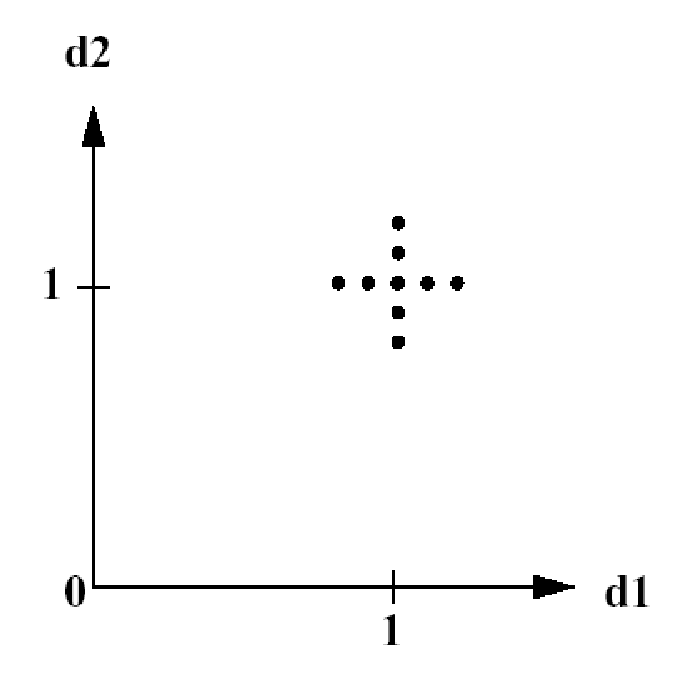
\includegraphics[scale=0.5]{images/centered_pstudy}
  \caption{Example centered parameter study.}
  \label{ps:figure01}
\end{figure}


\section{Multidimensional Parameter Study}\label{ps:multidimensional}

The multidimensional parameter study computes response data sets for
an $n$-dimensional hypergrid of points. Each variable is partitioned
into equally spaced intervals between its upper and lower bounds (see
Section~\ref{ps:overview:bounds}), and each combination of the values
defined by these partitions is evaluated.  As for the vector and
centered studies described in Sections~\ref{ps:vector}
and~\ref{ps:centered}, partitioning occurs using the actual variable
values for continuous and discrete range variables, but occurs within
the space of valid indices for discrete set variables (integer or
real).  The number of function evaluations performed in the study is:
\begin{equation}
  \prod_{i=1}^{n}(\hbox{\texttt{partitions}}_{i}+1)
  \label{ps:equation01}
\end{equation}

The partitions information is specified using the \texttt{partitions}
specification, which provides an integer list of the number of
partitions for each variable (i.e., \texttt{partitions}$_{i}$). Since
the Initial Values will not be used, they need not be specified.

In a two variable example problem with \texttt{d1} $\in$ [0,2] and 
\texttt{d2} $\in$ [0,3] (as defined by the upper and lower bounds 
from the variables specification) and with \texttt{partitions} =
(2,3), the interval [0,2] is divided into two equal-sized partitions
and the interval [0,3] is divided into three equal-sized partitions. 
This two-dimensional grid, shown in Figure~\ref{ps:figure02}, would 
result in the following twelve function evaluations:
\begin{figure}
  \centering
  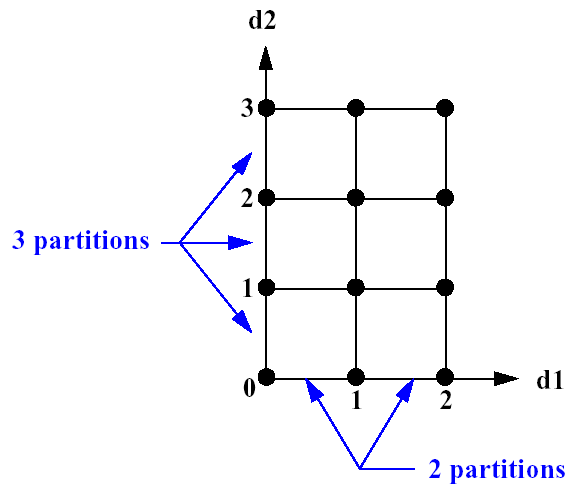
\includegraphics[scale=0.5]{images/multi_d_pstudy}
  \caption{Example multidimensional parameter study}
  \label{ps:figure02}
\end{figure}

\begin{small}
\begin{verbatim}
    Parameters for function evaluation 1:
                          0.0000000000e+00 d1   
                          0.0000000000e+00 d2   
    Parameters for function evaluation 2:
                          1.0000000000e+00 d1   
                          0.0000000000e+00 d2   
    Parameters for function evaluation 3:
                          2.0000000000e+00 d1   
                          0.0000000000e+00 d2   
    Parameters for function evaluation 4:
                          0.0000000000e+00 d1   
                          1.0000000000e+00 d2   
    Parameters for function evaluation 5:
                          1.0000000000e+00 d1   
                          1.0000000000e+00 d2   
    Parameters for function evaluation 6:
                          2.0000000000e+00 d1   
                          1.0000000000e+00 d2   
    Parameters for function evaluation 7:
                          0.0000000000e+00 d1   
                          2.0000000000e+00 d2   
    Parameters for function evaluation 8:
                          1.0000000000e+00 d1   
                          2.0000000000e+00 d2   
    Parameters for function evaluation 9:
                          2.0000000000e+00 d1   
                          2.0000000000e+00 d2   
    Parameters for function evaluation 10:
                          0.0000000000e+00 d1   
                          3.0000000000e+00 d2   
    Parameters for function evaluation 11:
                          1.0000000000e+00 d1   
                          3.0000000000e+00 d2   
    Parameters for function evaluation 12:
                          2.0000000000e+00 d1   
                          3.0000000000e+00 d2
\end{verbatim}
\end{small}

The first example shown in this User's Manual is a multi-dimensional
parameter study. See Section~\ref{tutorial:examples:param_study}.

\section{Usage Guidelines}\label{ps:usage}

Parameter studies, classical design of experiments (DOE),
design/analysis of computer experiments (DACE), and sampling methods
share the purpose of exploring the parameter space.  If directed
studies with a defined structure are desired, then parameter study
methods are recommended. For example, a quick assessment of the
smoothness of a response function is best addressed with a vector or
centered parameter study. Also, performing local sensitivity analysis
is best addressed with these methods. A multi-dimensional parameter 
study may be used to generate grid points for plotting response surfaces.
For guidance on DACE and sampling methods, in contrast to parameter 
studies, see Section~\ref{dace:usage}.
 
\section{Example: Vector Parameter Study with Rosenbrock}

This section demonstrates vector on the Rosenbrcok test function
described in Additional Examples.  An example of multidim is in
tutorial.

In addition to the multidimensional parameter study, Dakota can
perform a vector parameter study, i.e., a parameter study between any
two design points in an \emph{n}-dimensional parameter space.

An input file for the vector parameter study is shown in Figure~
\ref{additional:rosenbrock_vector}. The primary differences
between this input file and the previous input file are found in the
\emph{variables} and \emph{method} sections. In the variables section,
the keywords for the bounds are removed and replaced with the keyword
\texttt{initial\_point} that specifies the starting point for the
parameter study. In the method section, the
\texttt{vector\_parameter\_study} keyword is used. The
\texttt{final\_point} keyword indicates the stopping point for the
parameter study, and \texttt{num\_steps} specifies the number of steps
taken between the initial and final points in the parameter study.

\begin{figure}[ht!]
  \centering
  \begin{bigbox}
    \begin{small}
      \verbatimtabinput[8]{dakota_rosenbrock_vector.in}
    \end{small}
  \end{bigbox}
  \caption{Rosenbrock vector parameter study example: the Dakota input
  file.}
  \label{additional:rosenbrock_vector}
\end{figure}

The vector parameter study example problem is executed using the command
\begin{small}
\begin{verbatim}
    dakota dakota_rosenbrock_vector.in > vector.out
\end{verbatim}
\end{small}

Figure~\ref{additional:rosenbrock_vector_graphics}(a) shows the
graphics output created by Dakota. For this study, the simple Dakota
graphics are more useful for visualizing the
results. Figure~\ref{additional:rosenbrock_vector_graphics}(b)
shows the locations of the 11 sample points generated in this study.
It is evident from these figures that the parameter study starts
within the banana-shaped valley, marches up the side of the hill, and
then returns to the valley. The output file \texttt{vector.out.sav} is
provided in the \texttt{Dakota/examples/tutorial} directory.

In addition to the vector and multidimensional examples shown, Dakota
also supports list and centered parameter study methods. Refer to
Chapter~\ref{ps} for additional information.

\begin{figure}[htp!]
  \centering
  \begin{tabular}{c}
  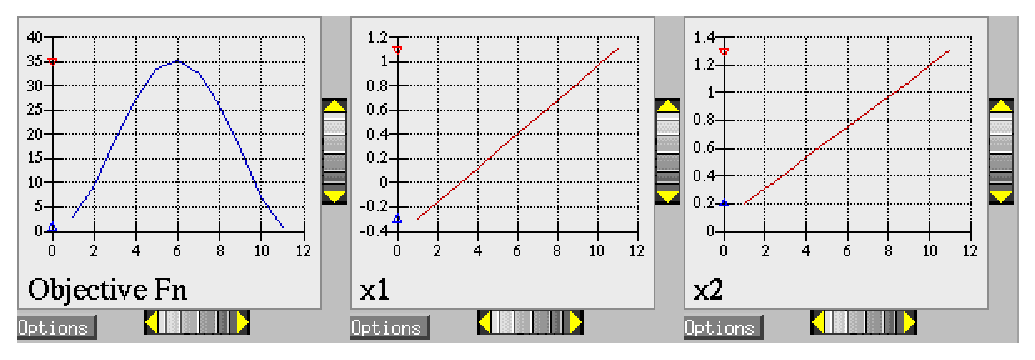
\includegraphics[width=\textwidth]{images/dak_graphics_vector}\\
  (a)\\
  \qquad\\
  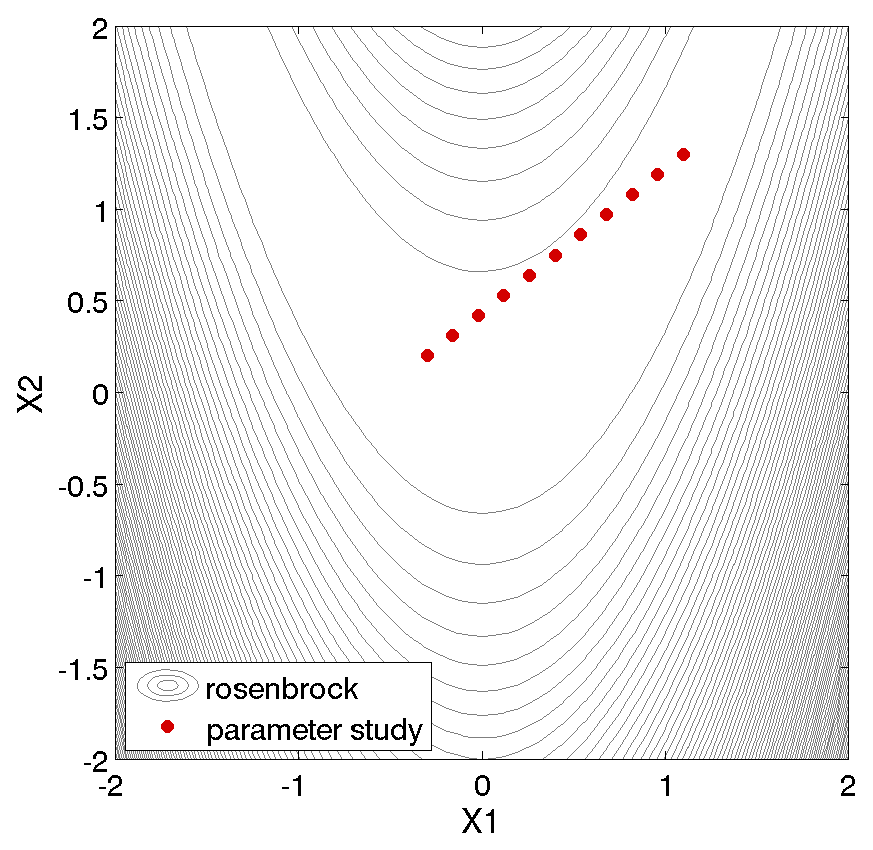
\includegraphics[height=2.5in]{images/rosen_vect_pts} \\
  (b)
  \end{tabular}
  \caption{Rosenbrock vector parameter study example: (a) screen
    capture of the Dakota graphics and (b) location of the design
    points (dots) evaluated.}
  \label{additional:rosenbrock_vector_graphics}
\end{figure}

\chapter{Design of Experiments Capabilities}\label{dace}

\section{Overview}\label{dace:overview}

Classical design of experiments (DoE) methods and the more modern
design and analysis of computer experiments (DACE) methods are both
techniques which seek to extract as much trend data from a parameter
space as possible using a limited number of sample points. Classical
DoE techniques arose from technical disciplines that assumed some
randomness and nonrepeatability in field experiments (e.g.,
agricultural yield, experimental chemistry). DoE approaches such as
central composite design, Box-Behnken design, and full and fractional
factorial design generally put sample points at the extremes of the
parameter space, since these designs offer more reliable trend
extraction in the presence of nonrepeatability. DACE methods are
distinguished from DoE methods in that the nonrepeatability component
can be omitted since computer simulations are involved. In these
cases, space filling designs such as orthogonal array sampling and
Latin hypercube sampling are more commonly employed in order to
accurately extract trend information. Quasi-Monte Carlo sampling
techniques which are constructed to fill the unit hypercube with good
uniformity of coverage can also be used for DACE.

Dakota supports both DoE and DACE techniques. In common usage, only
parameter bounds are used in selecting the samples within the
parameter space. Thus, DoE and DACE can be viewed as special cases of
the more general probabilistic sampling for uncertainty quantification
(see following section), in which the DoE/DACE parameters are treated
as having uniform probability distributions. The DoE/DACE techniques
are commonly used for investigation of global response trends,
identification of significant parameters (e.g., main effects), and as
data generation methods for building response surface approximations.

Dakota includes several approaches sampling and design of experiments,
all implemented in included third-party software libraries. LHS
(Latin hypercube sampling)~\cite{Swi04} is a general-purpose sampling
package developed at Sandia that has been used by the DOE national
labs for several decades. DDACE (distributed design and analysis for
computer experiments) is a more recent package for computer
experiments developed at Sandia Labs~\cite{TonXX}. DDACE provides the
capability for generating orthogonal arrays, Box-Behnken designs,
Central Composite designs, and random designs. The FSUDace (Florida
State University's Design and Analysis of Computer Experiments)
package provides the following sampling techniques: quasi-Monte Carlo
sampling based on Halton or Hammersley sequences, and Centroidal
Voronoi Tessellation. Lawrence Livermore National Lab's PSUADE
(Problem Solving Environment for Uncertainty Analysis and Design
Exploration)~\cite{Ton05} includes several methods for model
exploration, but only the Morris screening method is exposed in
Dakota.

This chapter describes DDACE, FSUDace, and PSUADE, with a focus on
designing computer experiments. Latin Hypercube Sampling, also used in
uncertainty quantification, is discussed in Section~\ref{uq:sampling}.
\begin{comment}
The differences between sampling used in design of experiments and
sampling used in uncertainty quantification is discussed in more
detail in the following paragraphs. In brief, we consider design of
experiment methods to generate sets of uniform random variables on the
interval $[0,1]$. These sets are mapped to the lower/upper bounds of
the problem variables and then the response functions are evaluated at
the sample input points with the goal of characterizing the behavior
of the response functions over the input parameter ranges of
interest. Uncertainty quantification via LHS sampling, in contrast,
involves characterizing the uncertain input variables with probability
distributions such as normal, Weibull, triangular, etc., sampling from
the input distributions, and propagating the input uncertainties to
obtain a cumulative distribution function on the output. There is
significant overlap between design of experiments and sampling. Often,
both techniques can be used to obtain similar results about the
behavior of the response functions and about the relative importance
of the input variables.
\end{comment}

\section{Design of Computer Experiments}\label{dace:background}

What distinguishes design of {\em computer} experiments?  Computer
experiments are often different from physical experiments, such as
those performed in agriculture, manufacturing, or biology. In
physical experiments, one often applies the same \emph{treatment} or
\emph{factor level} in an experiment several times to get an
understanding of the variability of the output when that treatment is
applied. For example, in an agricultural experiment, several fields
(e.g., 8) may be subject to a low level of fertilizer and the same
number of fields may be subject to a high level of fertilizer to see
if the amount of fertilizer has a significant effect on crop
output. In addition, one is often interested in the variability of the
output within a treatment group: is the variability of the crop yields
in the low fertilizer group much higher than that in the high
fertilizer group, or not?

In physical experiments, the process we are trying to examine is stochastic:  
that is, the same treatment may result in different outcomes. 
By contrast, in computer experiments, often we have a deterministic code. 
If we run the code with a particular set of input parameters, the code 
will always produce the same output. There certainly are stochastic codes, 
but the main focus of computer experimentation has been on deterministic codes. 
Thus, in computer experiments we often do not have the need to do replicates 
(running the code with the exact same input parameters several times to see 
differences in outputs). Instead, a major concern in computer experiments is 
to create an experimental design which can sample a high-dimensional space 
in a representative way with a minimum number of samples. 
The number of factors or parameters that we wish to explore in computer 
experiments is usually much higher than physical experiments. 
In physical experiments, one may be interested in varying a few parameters, 
usually five or less, while in computer experiments we often have 
dozens of parameters of interest. Choosing the levels of these parameters 
so that the samples adequately explore the input space is a challenging 
problem. There are many experimental designs and sampling methods 
which address the issue of adequate and representative sample selection. 
%Classical experimental designs which are often used in physical experiments 
%include Central Composite designs and Box-Behnken designs.

There are many goals of running a computer experiment: one may want to 
explore the input domain or the design space and get a better understanding 
of the range in the outputs for a particular domain. Another objective is 
to determine which inputs have the most influence on the output, or how 
changes in the inputs change the output. This is usually called 
\emph{sensitivity analysis}. 
%Another goal is to compare the relative 
%importance of model input uncertainties on the uncertainty in the model 
%outputs, \emph{uncertainty analysis}. 
Another goal is to use the 
sampled input points and their corresponding output to create a 
\emph{response surface approximation} for the computer code. The response 
surface approximation (e.g., a polynomial regression model, a 
Gaussian-process/Kriging model, a neural net) can then be used to emulate 
the computer code. 
Constructing a response surface approximation is particularly important 
for applications where running a computational model is extremely expensive:  
the computer model may take 10 or 20 hours to run on a high performance 
machine, whereas the response surface model may only take a few seconds. 
Thus, one often optimizes the response surface model or uses it within a 
framework such as surrogate-based optimization. Response surface models 
are also valuable in cases where the gradient (first derivative) and/or 
Hessian (second derivative) information required by optimization techniques 
are either not available, expensive to compute, or inaccurate because the 
derivatives are poorly approximated or the function evaluation is itself 
noisy due to roundoff errors. Furthermore, many optimization methods 
require a good initial point to ensure fast convergence or to converge to 
good solutions (e.g. for problems with multiple local minima). Under these 
circumstances, a good design of computer experiment framework coupled with 
response surface approximations can offer great advantages. 

In addition to the sensitivity analysis and response 
surface modeling mentioned above, we also may want to do 
\emph{uncertainty quantification} on a computer model. 
Uncertainty quantification (UQ) refers to taking a particular set of 
distributions on the inputs, and propagating them through the model to 
obtain a distribution on the outputs. For example, if input parameter A 
follows a normal with mean 5 and variance 1, the computer produces a random 
draw from that distribution. If input parameter B follows a weibull 
distribution with alpha = 0.5 and beta = 1, the computer produces a random 
draw from that distribution. When all of the uncertain variables have 
samples drawn from their input distributions, we run the model with the 
sampled values as inputs. We do this repeatedly to build up a distribution 
of outputs. We can then use the cumulative distribution function of the 
output to ask questions such as:  what is the probability that the output is 
greater than 10?   What is the 99th percentile of the output?  

Note that sampling-based uncertainty quantification and design of
computer experiments are very similar. \emph{There is significant
overlap} in the purpose and methods used for UQ and for DACE. We have
attempted to delineate the differences within Dakota as follows: we
use the methods DDACE, FSUDACE, and PSUADE primarily for design of
experiments, where we are interested in understanding the main effects
of parameters and where we want to sample over an input domain to
obtain values for constructing a response surface. We use the
nondeterministic sampling methods \texttt{(sampling)} for
uncertainty quantification, where we are propagating specific input
distributions and interested in obtaining (for example) a cumulative
distribution function on the output. If one has a problem with no
distributional information, we recommend starting with a design of
experiments approach. Note that DDACE, FSUDACE, and PSUADE currently
do \emph{not} support distributional information: they take an upper
and lower bound for each uncertain input variable and sample within
that. The uncertainty quantification methods in
\texttt{sampling} (primarily Latin Hypercube sampling) offer the
capability to sample from many distributional types. The distinction
between UQ and DACE is somewhat arbitrary: both approaches often can
yield insight about important parameters and both can determine sample
points for response surface approximations.

Three software packages are available in Dakota for design of computer
experiments, DDACE (developed at Sandia Labs), FSUDACE (developed at
Florida State University), and PSUADE (LLNL).

\section{DDACE}\label{dace:ddace}

The Distributed Design and Analysis of Computer Experiments (DDACE)
package includes both classical design of experiments
methods~\cite{TonXX} and stochastic sampling methods. The classical
design of experiments methods in DDACE are central composite design
(CCD) and Box-Behnken (BB) sampling. A grid-based sampling
(full-factorial) method is also available. The stochastic methods are
orthogonal array sampling~\cite{Koe96} (which permits main effects
calculations), Monte Carlo (random) sampling, Latin hypercube
sampling, and orthogonal array-Latin hypercube sampling. While DDACE
LHS supports variables with normal or uniform distributions, only
uniform are supported through Dakota. Also DDACE does not allow
enforcement of user-specified correlation structure among the
variables.

The sampling methods in DDACE can be used alone or in conjunction with
other methods. For example, DDACE sampling can be used with both the
surrogate-based optimization strategy and the optimization under
uncertainty strategy. See Figure~\ref{adv_models:figure09} for an
example of how the DDACE settings are used in Dakota.

%More information on DDACE is available on the web at:
%\url{http://csmr.ca.sandia.gov/projects/ddace}

The following sections provide more detail about the sampling 
methods available for design of experiments in DDACE. 

\subsection{Central Composite Design}\label{dace:ccd}

A Box-Wilson Central Composite Design, commonly called a central
composite design (CCD), contains an embedded factorial or fractional
factorial design with center points that is augmented with a group of
'star points' that allow estimation of curvature. If the distance
from the center of the design space to a factorial point is $\pm$1
unit for each factor, the distance from the center of the design space
to a star point is $\pm\alpha$ with $\mid\alpha\mid > 1$. The precise
value of $\alpha$ depends on certain properties desired for the design and on
the number of factors involved. The CCD design is specified in Dakota
with the method command \texttt{dace central\_composite}.

As an example, with two input variables or factors, each having two 
levels, the factorial design is shown in Table~\ref{dace:table01} . 

\begin{table}[ht]
 \caption{Simple Factorial Design}
 \label{dace:table01}	
 \begin{center}
  \begin{tabular}{c|c}
  \hline
  Input 1            & Input 2         \\ \hline \hline 
  -1                 & -1             \\ \hline 
  -1                 & +1           \\ \hline
  +1                 & -1      \\ \hline
  +1                 & +1        \\ \hline
  \end{tabular}
\end{center}
\end{table}


With a CCD, the design in Table~\ref{dace:table01} would be augmented 
with the following points shown in Table~\ref{dace:table02} 
if $\alpha$ = 1.3. These points define a circle around the original  
factorial design.

\begin{table}[ht]
 \caption{Additional Points to make the factorial design a CCD}
 \label{dace:table02}
 \begin{center}
  \begin{tabular}{c|c}
  \hline
  Input 1            & Input 2         \\ \hline \hline 
  0                 & +1.3             \\ \hline 
  0                 & -1.3           \\ \hline
  1.3                 & 0     \\ \hline
  -1.3                 & 0       \\ \hline
  0                  & 0          \\ \hline
  \end{tabular}
\end{center}
\end{table}

Note that the number of sample points specified in a CCD,\texttt{samples},
is a function of the number of variables in the problem: 

\[
samples = 1 + 2*NumVar + 2^{NumVar}
\]

\subsection{Box-Behnken Design}\label{dace:bb}

The Box-Behnken design is similar to a Central Composite design, with
some differences. The Box-Behnken design is a quadratic design in
that it does not contain an embedded factorial or fractional factorial
design. In this design the treatment combinations are at the midpoints
of edges of the process space and at the center, as compared with CCD
designs where the extra points are placed at 'star points' on a circle
outside of the process space. Box-Behken designs are rotatable (or
near rotatable) and require 3 levels of each factor. The designs have
limited capability for orthogonal blocking compared to the central
composite designs. Box-Behnken requires fewer runs than CCD for 3
factors, but this advantage goes away as the number of factors
increases. The Box-Behnken design is specified in Dakota with the
method command \texttt{dace box\_behnken}.

Note that the number of sample points specified in a Box-Behnken design,
\texttt{samples}, is a function of the number of variables in the problem: 

\[
samples = 1 + 4*NumVar + (NumVar-1)/2
\]

\subsection{Orthogonal Array Designs}\label{dace:oas}

Orthogonal array (OA) sampling is a widely used technique for 
running experiments and systematically testing factor effects~\cite{Hed99}. 
An orthogonal array sample can be described as a 4-tuple $(m,n,s,r)$,
where $m$ is the number of sample points, $n$ is the number of input variables, 
$s$ is the number of symbols, and $r$ is the strength of the orthogonal array. 
The number of sample points, $m$, must be a multiple of the number of symbols, 
$s$. The number of symbols refers to the number of levels per input variable. 
The strength refers to the number of columns where we are guaranteed to 
see all the possibilities an equal number of times.

For example, Table~\ref{dace:table03} shows an orthogonal array of strength 2 for $m$ = 8, with 7 variables:

\begin{table}[ht]
 \caption{Orthogonal Array for Seven Variables}
 \label{dace:table03}
 \begin{center}
  \begin{tabular}{c|c|c|c|c|c|c}
  \hline
  Input 1 & Input 2 & Input 3 & Input 4 & Input 5 & Input 6 & Input 7\\ \hline \hline 
0 & 	0 &	0 &	0 & 	0 &	0 &	0  \\ \hline
0 &	0 &	0 &	1 &	1 &	1 &	1   \\ \hline
0 &	1 & 	1 & 	0 & 	0 &	1 &	1   \\ \hline
0 &	1 &	1 &	1 &	1 &	0 &	0    \\ \hline
1 &	0 &	1 &	0 &	1 &	0 &	1   \\ \hline
1 &	0 &	1 &	1 &	0 &	1 &	0 \\ \hline
1 &	1 &	0 &	0 &	1 &	1 &	0 \\ \hline
1 &	1 &	0 &	1 &	0 &	0 &	1 \\ \hline

  \end{tabular}
\end{center}
\end{table}


If one picks any two columns, say the first and the third, note that 
each of the four possible rows we might see there,
0 0,       0 1,       1 0,       1 1,
appears exactly the same number of times, twice in this case.

DDACE creates orthogonal arrays of strength 2. Further, 
the OAs generated by DDACE do not treat the factor levels as one 
fixed value (0 or 1 in the above example). Instead, once a level 
for a variable is determined in the array,  DDACE 
samples a random variable from within that level.
The orthogonal array design is specified in 
Dakota with the method command \texttt{dace oas}. 

The orthogonal array method in DDACE is the only method that 
allows for the calculation of main effects, specified with the 
command \texttt{main\_effects}. Main effects is a sensitivity analysis 
method which identifies the input variables that have the most 
influence on the output. In main effects, the idea is to look 
at the mean of the response function when variable A (for example) 
is at level 1 vs. when variable A is at level 2 or level 3. 
If these mean responses of the output are statistically significantly 
different at different levels of variable A, this is an indication that 
variable A has a significant effect on the response. 
The orthogonality of the columns is critical in performing 
main effects analysis, since the column orthogonality means 
that the effects of the other variables 'cancel out' when 
looking at the overall effect from one variable at its different 
levels. There are ways of developing orthogonal arrays to calculate 
higher order interactions, such as two-way interactions (what 
is the influence of Variable A * Variable B on the output?), but this is 
not available in DDACE currently. At present, one way interactions 
are supported in the calculation of orthogonal array main effects within DDACE.
The main effects are presented as a series of ANOVA tables. 
For each objective function and constraint, the decomposition of variance 
of that objective or constraint is presented as a function of the 
input variables. The p-value in the ANOVA table is used to indicate 
if the input factor is significant. The p-value is the probability that 
you would have obtained samples more extreme than you did if the input 
factor has no effect on the response. For example, if you set a level 
of significance at 0.05 for your p-value, and the actual p-value is 0.03, 
then the input factor has a significant effect on the response. 

\subsection{Grid Design}\label{dace:grid}

In a grid design, a grid is placed over the input variable space. 
This is very similar to a multi-dimensional parameter study where 
the samples are taken over a set of partitions on each variable 
(see Section~\ref{ps:multidimensional}). The main difference is 
that in grid sampling, a small random perturbation is added 
to each sample value so that the grid points are not on a perfect grid. 
This is done to help capture certain features in the output such as periodic
functions. A purely structured grid, with the samples exactly on the grid 
points, has the disadvantage of not being able to capture important features 
such as periodic functions with relatively high frequency (due to aliasing). 
Adding a random perturbation to the grid samples helps remedy this problem.

Another disadvantage with grid sampling is that the number of sample points 
required depends exponentially on the input dimensions. In grid sampling, 
the number of samples is the number of symbols (grid partitions) raised 
to the number of variables. For example, if there are 2 variables, each 
with 5 partitions, the number of samples would be $5^2$. In this 
case, doubling the number of variables squares the sample size. 
The grid design is specified in 
Dakota with the method command \texttt{dace grid}.

\subsection{Monte Carlo Design}\label{dace:mc}

Monte Carlo designs simply involve pure Monte-Carlo random sampling 
from uniform distributions between the lower and upper bounds on each 
of the input variables. Monte Carlo designs, specified by 
\texttt{dace random}, are a way to generate a set of random samples 
over an input domain.

\subsection{LHS Design}\label{dace:lhs}

DDACE offers the capability to generate Latin Hypercube designs. 
For more information on Latin Hypercube sampling, see 
Section~\ref{uq:sampling}. Note that the version of LHS in DDACE 
generates uniform samples (uniform between the variable bounds). 
The version of LHS offered with nondeterministic sampling can generate 
LHS samples according to a number of distribution types, including 
normal, lognormal, weibull, beta, etc. To specify the DDACE version 
of LHS, use the method command \texttt{dace lhs}.

\subsection{OA-LHS Design}\label{dace:oalhs}

DDACE offers a hybrid design which is combination of an orthogonal
array and a Latin Hypercube sample. This design is specified with the
method command \texttt{dace oa\_lhs}. This design has the advantages
of both orthogonality of the inputs as well as stratification of the
samples (see~\cite{Owe92}).

\section{FSUDace}\label{dace:fsudace}

The Florida State University Design and Analysis of Computer
Experiments (FSUDace) package provides quasi-Monte Carlo sampling
(Halton and Hammersley) and Centroidal Voronoi Tessellation (CVT)
methods. All three methods natively generate sets of uniform random
variables on the interval $[0,1]$ (or in Dakota, on user-specified
uniform intervals).

The quasi-Monte Carlo and CVT methods are designed with the goal of
low discrepancy. Discrepancy refers to the nonuniformity of the sample
points within the unit hypercube. Low discrepancy sequences tend to
cover the unit hypercube reasonably uniformly. Quasi-Monte Carlo
methods produce low discrepancy sequences, especially if one is
interested in the uniformity of projections of the point sets onto
lower dimensional faces of the hypercube (usually 1-D: how well do the
marginal distributions approximate a uniform?) CVT does very well
volumetrically: it spaces the points fairly equally throughout the
space, so that the points cover the region and are isotropically
distributed with no directional bias in the point placement. There are
various measures of volumetric uniformity which take into account the
distances between pairs of points, regularity measures, etc. Note that
CVT does not produce low-discrepancy sequences in lower dimensions,
however: the lower-dimension (such as 1-D) projections of CVT can have
high discrepancy.

The quasi-Monte Carlo sequences of Halton and Hammersley are
deterministic sequences determined by a set of prime bases.
A Halton design is specified in Dakota with the method command 
\texttt{fsu\_quasi\_mc halton}, and the Hammersley design is 
specified with the command \texttt{fsu\_quasi\_mc hammersley}.
For more details about the input specification, see the Reference Manual.
CVT points tend to arrange themselves in a pattern
of cells that are roughly the same shape. To produce CVT
points, an almost arbitrary set of initial points is chosen, and then
an internal set of iterations is carried out. These iterations
repeatedly replace the current set of sample points by an estimate of
the centroids of the corresponding Voronoi subregions~\cite{Du99}.
A CVT design is specified in Dakota with the method command
\texttt{fsu\_cvt}.

The methods in FSUDace are useful for design of experiments because 
they provide good coverage of the input space, thus allowing global 
sensitivity analysis. 

\section{PSUADE MOAT}\label{dace:psuade}

PSUADE (Problem Solving Environment for Uncertainty Analysis and
Design Exploration) is a Lawrence Livermore National Laboratory tool
for metamodeling, sensitivity analysis, uncertainty quantification,
and optimization. Its features include non-intrusive and parallel
function evaluations, sampling and analysis methods, an integrated
design and analysis framework, global optimization, numerical
integration, response surfaces (MARS and higher order regressions),
graphical output with Pgplot or Matlab, and fault
tolerance~\cite{Ton05}. Dakota includes a prototype interface to its
Morris One-At-A-Time (MOAT) screening method, a valuable tool for
global sensitivity (including interaction) analysis.

The Morris One-At-A-Time method, originally proposed by
M.~D. Morris~\cite{Mor91}, is a screening method, designed to explore
a computational model to distinguish between input variables that have
negligible, linear and additive, or nonlinear or interaction effects
on the output. The computer experiments performed consist of
individually randomized designs which vary one input factor at a time
to create a sample of its elementary effects.

With MOAT, each dimension of a $k-$dimensional input space is
uniformly partitioned into $p$ levels, creating a grid of $p^k$ points
${\bf x} \in \mathbb{R}^k$ at which evaluations of the model $y({\bf
x})$ might take place. An elementary effect corresponding to input
$i$ is computed by a forward difference
\begin{equation}
d_i({\bf x}) = \frac{y({\bf x} + \Delta {\bf e}_i) - y({\bf x})}{\Delta},
\end{equation}
where $e_i$ is the $i^{\mbox{\scriptsize th}}$ coordinate vector, and
the step $\Delta$ is typically taken to be large (this is not intended
to be a local derivative approximation). In the present
implementation of MOAT, for an input variable scaled to $[0,1]$,
$\Delta = \frac{p}{2(p-1)}$, so the step used to find elementary
effects is slightly larger than half the input range.

The distribution of elementary effects $d_i$ over the input space
characterizes the effect of input $i$ on the output of interest.
After generating $r$ samples from this distribution, their mean,
\begin{equation}
\mu_i = \frac{1}{r}\sum_{j=1}^{r}{d_i^{(j)}},
\end{equation}
modified mean
\begin{equation}
\mu_i^* = \frac{1}{r}\sum_{j=1}^{r}{|d_i^{(j)}|},
\end{equation}
(using absolute value) and standard deviation
\begin{equation}
\sigma_i = \sqrt{ \frac{1}{r}\sum_{j=1}^{r}{ \left(d_i^{(j)} - \mu_i
\right)^2} }
\end{equation}
are computed for each input $i$. The mean and modified mean give an
indication of the overall effect of an input on the output. Standard
deviation indicates nonlinear effects or interactions, since it is an
indicator of elementary effects varying throughout the input space.

The MOAT method is selected with method keyword {\tt psuade\_moat} as
shown in the sample Dakota input deck in Figure~\ref{FIG:moat_input}.
The number of samples ({\tt samples}) must be a positive integer
multiple of (number of continuous design variables $k$ + 1) and will
be automatically adjusted if misspecified. The number of partitions
({\tt partitions}) applies to each variable being studied and must be
odd (the number of MOAT levels $p$ per variable is partitions + 1,
similar to Dakota multidimensional parameter studies). This will also
be adjusted at runtime as necessary. Finite user-specified lower and
upper bounds are required and will be scaled as needed by the method.
For more information on use of MOAT sampling, see the Morris example
in Section~\ref{additional:morris}, or Saltelli, et al.~\cite{Sal04}.

\begin{figure}
  \centering \begin{bigbox} \begin{small}
  \verbatimtabinput[8]{morris_ps_moat.in} \end{small} \end{bigbox}
\caption{Dakota input file showing the Morris One-at-a-Time method --
see {\tt Dakota/examples/users/morris\_ps\_moat.in} }
\label{FIG:moat_input}
\end{figure}

\section{Sensitivity Analysis}\label{dace:sa}

\subsection{Sensitivity Analysis Overview}\label{dace:sa:overview}

In many engineering design applications, sensitivity analysis
techniques and parameter study methods are useful in identifying which
of the design parameters have the most influence on the response
quantities. This information is helpful prior to an optimization study
as it can be used to remove design parameters that do not strongly
influence the responses. In addition, these techniques can provide
assessments as to the behavior of the response functions (smooth or
nonsmooth, unimodal or multimodal) which can be invaluable in
algorithm selection for optimization, uncertainty quantification, and
related methods. In a post-optimization role, sensitivity information
is useful is determining whether or not the response functions are
robust with respect to small changes in the optimum design point.

In some instances, the term sensitivity analysis is used in a local
sense to denote the computation of response derivatives at a point.
These derivatives are then used in a simple analysis to make design
decisions. Dakota supports this type of study through numerical
finite-differencing or retrieval of analytic gradients computed within
the analysis code. The desired gradient data is specified in the
responses section of the Dakota input file and the collection of this
data at a single point is accomplished through a parameter study
method with no steps. This approach to sensitivity analysis should be
distinguished from the activity of augmenting analysis codes to
internally compute derivatives using techniques such as direct or
adjoint differentiation, automatic differentiation (e.g., ADIFOR), or
complex step modifications. These sensitivity augmentation activities
are completely separate from Dakota and are outside the scope of this
manual. However, once completed, Dakota can utilize these analytic
gradients to perform optimization, uncertainty quantification, and
related studies more reliably and efficiently.

In other instances, the term sensitivity analysis is used in a more
global sense to denote the investigation of variability in the
response functions. Dakota supports this type of study through
computation of response data sets (typically function values only, but
all data sets are supported) at a series of points in the parameter
space. The series of points is defined using either a vector, list,
centered, or multidimensional parameter study method. For example, a
set of closely-spaced points in a vector parameter study could be used
to assess the smoothness of the response functions in order to select
a finite difference step size, and a set of more widely-spaced points
in a centered or multidimensional parameter study could be used to
determine whether the response function variation is likely to be
unimodal or multimodal. See Chapter~\ref{ps} for additional
information on these methods. These more global approaches to
sensitivity analysis can be used to obtain trend data even in
situations when gradients are unavailable or unreliable, and they are
conceptually similar to the design of experiments methods and sampling
approaches to uncertainty quantification described in the following
sections.

\subsection{Assessing Sensitivity with DACE}\label{dace:sa:assessing}

Like parameter studies (see Chapter~\ref{ps}), the DACE techniques are
useful for characterizing the behavior of the response functions of
interest through the parameter ranges of interest. In addition to
direct interrogation and visualization of the sampling results, a
number of techniques have been developed for assessing the parameters
which are most influential in the observed variability in the response
functions. One example of this is the well-known technique of scatter
plots, in which the set of samples is projected down and plotted
against one parameter dimension, for each parameter in turn. Scatter
plots with a uniformly distributed cloud of points indicate parameters
with little influence on the results, whereas scatter plots with a
defined shape to the cloud indicate parameters which are more
significant. Related techniques include analysis of variance
(ANOVA)~\cite{Mye95} and main effects analysis, in which the parameters
which have the greatest influence on the results are identified from
sampling results. Scatter plots and ANOVA may be accessed through
import of Dakota tabular results (see Section~\ref{output:tabular})
into external statistical analysis programs such as S-plus, Minitab,
etc.

Running any of the design of experiments or sampling methods allows
the user to save the results in a tabular data file, which then can be
read into a spreadsheet or statistical package for further analysis.
In addition, we have provided some functions to help determine the
most important variables.

We take the definition of uncertainty analysis from~\cite{Sal04}: 
``The study of how uncertainty in the output of a model can be 
apportioned to different sources of uncertainty in the model input.''

As a default, Dakota provides correlation analyses when running LHS.
Correlation tables are printed with the simple, partial, and rank
correlations between inputs and outputs. These can be useful to get a
quick sense of how correlated the inputs are to each other, and how
correlated various outputs are to inputs. The correlation analyses are
explained further in Chapter~\ref{uq:sampling}.

We also have the capability to calculate sensitivity indices through
Variance-based Decomposition (VBD). Variance-based decomposition 
is a global sensitivity method that summarizes how the uncertainty 
in model output can be apportioned to uncertainty in individual 
input variables. VBD uses two primary measures, the main effect 
sensitivity index $S_{i}$ and the total effect index $T_{i}$. The 
main effect sensitivity 
index corresponds to the fraction of the uncertainty in the output, $Y$, 
that can be attributed to input $x_{i}$ alone. The total effects index 
corresponds to the fraction of the uncertainty in 
the output, $Y$, that can be attributed to input $x_{i}$ and its 
interactions with other variables. The main effect sensitivity index
compares the variance of the conditional expectation
$Var_{x_{i}}[E(Y|x_{i})]$ against the total variance $Var(Y)$.
Formulas for the indices are: 

\begin{equation}
S_{i}=\frac{Var_{x_{i}}[E(Y|x_{i})]}{Var(Y)} \label{eq:VBD_Si}
\end{equation}

and 
\begin{equation}
T_{i}=\frac{E(Var(Y|x_{-i}))}{Var(Y)}=\frac{Var(Y)-Var(E[Y|x_{-i}])}{Var(Y)} \label{eq:VBD_Ti}
\end{equation}

where $Y=f({\bf x})$ and ${x_{-i}=(x_{1},...,x_{i-1},x_{i+1},...,x_{m})}$.

The calculation of $S_{i}$ and $T_{i}$ requires the evaluation of 
m-dimensional integrals which are typically approximated by Monte-Carlo 
sampling. More details on the
calculations and interpretation of the sensitivity indices can be
found in~\cite{Sal04}. In Dakota version 5.1, we have 
improved calculations for the calculation of the $S_{i}$ and $T_{i}$ 
indices when using sampling. The implementation details of these 
calculatiosn are provided in~\cite{Weirs10}. 
VBD can be specified for any of the sampling or DACE methods using the 
command \texttt{variance\_based\_decomposition}.
Note that VBD is extremely computationally intensive when using sampling 
since replicated sets of sample values are evaluated. If the
user specified a number of samples, $N$, and a number of
nondeterministic variables, $M$, variance-based decomposition
requires the evaluation of $N(M+2)$ samples. To obtain
sensitivity indices that are reasonably accurate, we recommend that
$N$, the number of samples, be at least one hundred and
preferably several hundred or thousands. Because of the computational
cost, variance-based decomposition is turned off as a default
for sampling or DACE. Another alternative, however, is to obtain 
these indices using one of the stochastic expansion methods 
described in Section~\ref{uq:expansion}. The calculation 
of the indices using expansion methods is much more efficient 
since the VBD indices are analytic functions of the coefficients 
in the stochastic expansion. The paper by Weirs et al.~\cite{Weirs10}
compares different methods for calculating the sensitivity 
indices for nonlinear problems with significant interaction effects.

In terms of interpretation of the sensitivity indices, a larger value of
the sensitivity index, $S_{i}$,
means that the uncertainty in the input variable $i$ has a
larger effect on the variance of the output. Note that the 
sum of the main effect indices will be less than or equal to one. 
If the sum of the main effect indices is much less than one, 
it indicates that there are significant two-way, three-way, or higher
order interactions that contribute significantly to the variance. 
There is no requirement that the sum of the total effect indices 
is one:  in most cases, the sum of the total effect indices will be 
greater than one. An example of the Main and Total effects 
indices as calculated by Dakota using sampling is shown 
in Figure~\ref{fig:dace:vbd}

\begin{figure}[ht!]
\centering
\begin{bigbox}
\begin{small}
\begin{verbatim}
Global sensitivity indices for each response function:
response_fn_1 Sobol indices:
                                  Main             Total
                      4.7508913283e-01  5.3242162037e-01 uuv_1
                      3.8112392892e-01  4.9912486515e-01 uuv_2
\end{verbatim}
\end{small}
\end{bigbox}
\caption{Dakota output for Variance-based Decomposition} 
\label{fig:dace:vbd}
\end{figure}

Finally, we have the capability to calculate a set of quality metrics 
for a particular input sample. These quality metrics measure 
various aspects relating to the volumetric spacing of the samples: 
are the points equally spaced, do they cover the region, are they 
isotropically distributed, do they have directional bias, etc.? 
The quality metrics are explained in more detail in the Reference Manual.

\section{DOE Usage Guidelines}\label{dace:usage}

Parameter studies, classical design of experiments (DOE),
design/analysis of computer experiments (DACE), and sampling methods
share the purpose of exploring the parameter space. When a global
space-filling set of samples is desired, then the DOE, DACE, and
sampling methods are recommended. These techniques are useful for
scatter plot and variance analysis as well as surrogate model
construction. 

The distinction between DOE and DACE methods is that the
former are intended for physical experiments containing an element of
nonrepeatability (and therefore tend to place samples at the extreme
parameter vertices), whereas the latter are intended for repeatable
computer experiments and are more space-filling in nature. 

The distinction between DOE/DACE and sampling is drawn based on the
distributions of the parameters. DOE/DACE methods typically assume
uniform distributions, whereas the sampling approaches in Dakota
support a broad range of probability distributions. 

To use \texttt{sampling} in design of experiments mode (as opposed to 
uncertainty quantification mode), the \texttt{all\_variables} flag
should be included in the method specification of the Dakota input
file.

Design of experiments method selection recommendations are summarized
in Table~\ref{dace:usage:table}.

\begin{table}[hbp]
\centering
\caption{Guidelines for selection of parameter study, DOE, DACE, and
sampling methods.}
\label{dace:usage:table}\vspace{2mm}
\begin{tabular}{|c|c|c|}
\hline
\textbf{Method} & \textbf{Applications} & \textbf{Applicable Methods} \\
\textbf{Classification} & & \\
\hline
parameter study & sensitivity analysis,                       & centered\_parameter\_study, \\
                & directed parameter space investigations     & list\_parameter\_study, \\
                &                                             & multidim\_parameter\_study, \\
                &                                             & vector\_parameter\_study \\
                   &                                             & \\
\hline
classical design & physical experiments                       & dace (box\_behnken, \\
of experiments   & (parameters are uniformly distributed)     & central\_composite) \\
                   &                                             & \\
\hline
design of computer & variance analysis,                       & dace (grid, random,
                                                                oas, lhs, oa\_lhs), \\
experiments        & space filling designs                    & fsu\_quasi\_mc (halton, 
                                                                hammersley), \\
                   & (parameters are uniformly distributed)   & fsu\_cvt, psuade\_moat \\
                   &                                             & \\
\hline
sampling           & space filling designs                    & sampling (Monte Carlo or LHS) \\
                   & (parameters have general probability distributions) & with all\_variables flag \\
                   &                                             & \\
\hline
\end{tabular}
\end{table}

\chapter{Uncertainty Quantification Capabilities}\label{uq}

\section{Overview}\label{uq:overview}

At a high level, uncertainty quantification (UQ) or nondeterministic
analysis is the process of characterizing input uncertainties, forward
propagating these uncertainties through a computational model, and
performing statistical or interval assessments on the resulting
responses. This process determines the effect of uncertainties and
assumptions on model outputs or results. In Dakota, uncertainty
quantification methods specifically focus on the forward propagation
part of the process, where probabilistic or interval information on
parametric inputs are mapped through the computational model to assess
statistics or intervals on outputs. For an overview of these
approaches for engineering applications, consult~\cite{Hal00}.

UQ is related to sensitivity analysis in that the common goal is to
gain an understanding of how variations in the parameters affect the
response functions of the engineering design problem. However, for UQ,
some or all of the components of the parameter vector, are considered
to be uncertain as specified by particular probability distributions
(e.g., normal, exponential, extreme value), or other uncertainty
structures. By assigning specific distributional structure to the
inputs, distributional structure for the outputs (i.e, response
statistics) can be inferred.  This migrates from an analysis that is
more {\em qualitative} in nature, in the case of sensitivity analysis,
to an analysis that is more rigorously {\em quantitative}.

UQ methods are often distinguished by their ability to propagate
aleatory or epistemic input uncertainty characterizations, where
aleatory uncertainties are irreducible variabilities inherent in
nature and epistemic uncertainties are reducible uncertainties
resulting from a lack of knowledge. Since sufficient data is generally
available for aleatory uncertainties, probabilistic methods are
commonly used for computing response distribution statistics based on
input probability distribution specifications. Conversely, for
epistemic uncertainties, any use of probability distributions is based
on subjective knowledge rather than objective data, and we may
alternatively explore nonprobabilistic methods based on interval
specifications.

\subsection{Summary of Dakota UQ Methods}\label{uq:overview:methods}

Dakota contains capabilities for performing nondeterministic analysis
with both types of input uncertainty. These UQ methods have been
developed by Sandia Labs, in conjunction with collaborators in
academia~\cite{Gha99,Gha91,Eld05,Tang10a}.

The aleatory UQ methods in Dakota include various sampling-based
approaches (e.g., Monte Carlo and Latin Hypercube sampling), local and
global reliability methods, and stochastic expansion (polynomial chaos
expansions and stochastic collocation) approaches. The epistemic UQ
methods include local and global interval analysis and Dempster-Shafer
evidence theory. These are summarized below and then described in more
depth in subsequent sections of this chapter. Dakota additionally
supports mixed aleatory/epistemic UQ via interval-valued probability,
second-order probability, and Dempster-Shafer theory of
evidence. These involve advanced model recursions and are described in
Section~\ref{adv_models:mixed_uq}.

%In addition, future extensions to the DDACE package will make it 
%applicable to general UQ problems, which will augment the Dakota/UQ 
%capabilities.
%Uncertainty quantification methods (also referred to as
%nondeterministic analysis methods) in the Dakota/UQ system involve the
%computation of probabilistic information about response functions
%based on sets of simulations taken from the specified probability
%distributions for uncertain parameters. That is, 

%The impact on the response functions due to the probabilistic nature
%of the parameters is often estimated using a sampling-based approach
%such as Monte Carlo sampling or one of its variants (latin hypercube,
%quasi-Monte Carlo, Markov-chain Monte Carlo, etc.). In these sampling
%approaches, a random number generator is used to select different
%values of the parameters with probability specified by their
%probability distributions. This is the point that distinguishes UQ
%sampling from DoE/DACE sampling, in that the former supports general
%probabilistic descriptions of the parameter set and the latter
%generally supports only a bounded parameter space description. A
%particular set of parameter values is often called a \emph{sample
%point}, or simply a \emph{sample}. With Monte Carlo and Latin
%Hypercube sampling, the user may specify correlations among the input
%sample points. After a user-selected number of sample points has been
%generated, the response functions for each sample are evaluated. Then,
%a statistical analysis is performed on the response function values to
%yield information on their characteristics. While this approach is
%straightforward, and readily amenable to parallel computing, it can be
%computationally expensive depending on the accuracy requirements of
%the statistical information (which links directly to the number of
%sample points).

%Finally, when the input uncertainties are poorly characterized, then
%epistemic uncertainty methods, such as second-order probability or
%Dempster-Shafer theory of evidence, can be used to compute intervals
%of potential probability values. The second-order probability
%approach performs an ensemble of aleatory UQ analyses, one for each
%realization of the epistemic parameter set. The ensemble of CDF/CCDF
%curves generates what is known as a ``horse-tail'' plot.
%Dempster-Shafer, on the other hand, directly generates probability
%bounds, known as the belief and plausibility functions.

%This chapter has extensive details on various Dakota UQ methods, but
%here is a high-level summary of available capabilities:

% BMA TODO: Considerably shorten the following descriptions, moving
% text to later sections if needed.

\textbf{LHS (Latin Hypercube Sampling)}: This package provides both
Monte Carlo (random) sampling and Latin Hypercube sampling methods,
which can be used with probabilistic variables in Dakota that have the
following distributions: normal, lognormal, uniform, loguniform,
triangular, exponential, beta, gamma, gumbel, frechet, weibull, poisson, 
binomial, negative binomial, geometric, hypergeometric, and
user-supplied histograms. In addition, LHS accounts for correlations
among the variables~\cite{Ima84}, which can be used to accommodate a
user-supplied correlation matrix or to minimize correlation when a
correlation matrix is not supplied. 
%The LHS package currently serves
%two purposes: (1) it can be used for uncertainty quantification by
%sampling over uncertain variables characterized by probability
%distributions, or (2) it can be used in a DACE mode in which any
%design and state variables are treated as having uniform distributions
%(see the \texttt{active all} view override in the Dakota Reference
%Manual~\cite{RefMan}). The LHS package historically came in two
%versions: ``old'' (circa 1980) and ``new'' (circa 1998), but presently
%only the latter is supported in Dakota, requiring a Fortran 90
%compiler. This ``new'' LHS is available under a separate GNU Lesser
%General Public License and is distributed with Dakota. 
In addition to a standard sampling study, we support the capability to perform 
``incremental'' LHS, where a user can specify an initial LHS study 
of N samples, and then re-run an additional incremental study which 
will double the number of samples (to 2N, with the first N being 
carried from the initial study). The full incremental sample of 
size 2N is also a Latin Hypercube, with proper stratification and 
correlation. 

\textbf{Reliability Methods}: This suite of methods includes both
local and global reliability methods. Local methods include first- and
second-order versions of the Mean Value method (MVFOSM and MVSOSM) and
a variety of most probable point (MPP) search methods, including the
Advanced Mean Value method (AMV and AMV$^2$), the iterated Advanced
Mean Value method (AMV+ and AMV$^2$+), the Two-point Adaptive
Nonlinearity Approximation method (TANA-3), and the traditional First
Order and Second Order Reliability Methods (FORM and
SORM)~\cite{Hal00}. The MPP search methods may be used in forward
(Reliability Index Approach (RIA)) or inverse (Performance Measure
Approach (PMA)) modes, as dictated by the type of level mappings. Each
of the MPP search techniques solve local optimization problems in
order to locate the MPP, which is then used as the point about which
approximate probabilities are integrated (using first- or second-order
integrations in combination with refinements based on importance
sampling).
% Reliability mappings may involve computing reliability and
% probability levels for prescribed response levels (forward
% reliability analysis, commonly known as the reliability index
% approach or RIA) or computing response levels for prescribed
% reliability and probability levels (inverse reliability analysis,
% commonly known as the performance measure approach or PMA).
% Approximation-based MPP search methods (AMV, AMV$^2$, AMV+,
% AMV$^2$+, and TANA) may be applied in either x-space or u-space, and
% mappings may involve either cumulative or complementary cumulative
% distribution functions.
Global reliability methods are designed to handle
nonsmooth and multimodal failure surfaces, by creating global
approximations based on Gaussian process models. They accurately
resolve a particular contour of a response function and then estimate
probabilities using multimodal adaptive importance sampling.

\textbf{Stochastic Expansion Methods}: %The objective of these
%techniques is to characterize the response of systems whose governing
%equations involve stochastic coefficients. 
The development of these techniques mirrors that of deterministic
finite element analysis utilizing the notions of projection,
orthogonality, and weak convergence~\cite{Gha99},~\cite{Gha91}. Rather
than estimating point probabilities, they form an approximation to the
functional relationship between response functions and their random
inputs, which provides a more complete uncertainty representation for
use in multi-code simulations. Expansion methods include polynomial
chaos expansions (PCE), which employ multivariate orthogonal
polynomials that are tailored to representing particular input
probability distributions, and stochastic collocation (SC), which
employs multivariate interpolation polynomials.  For PCE, expansion
coefficients may be evaluated using a spectral projection approach
(based on sampling, tensor-product quadrature, Smolyak sparse grid, or
cubature methods for numerical integration) or a regression approach
(least squares or compressive sensing). For SC, interpolants are
formed over tensor-product or sparse grids and may be local or global,
value-based or gradient-enhanced, and nodal or hierarchical. In global
value-based cases (Lagrange polynomials), the barycentric formulation
is used~\cite{BerTref04,Klimke05,Higham04} to improve numerical
efficiency and stability.  Both sets of methods provide analytic
response moments and variance-based metrics; however, CDF/CCDF
probabilities are evaluated numerically by sampling on the expansion.

\textbf{Importance Sampling}: Importance sampling is a method that 
allows one to estimate statistical quantities such as failure 
probabilities in a way that is more efficient than Monte Carlo 
sampling. The core idea in importance sampling is that one generates 
samples that are preferentially placed in important regions of the 
space (e.g. in or near the failure region or user-defined region
of interest), then appropriately weights the samples to obtain an 
unbiased estimate of the failure probability.

\textbf{Adaptive Sampling}: The goal in performing adaptive 
sampling is to construct a surrogate
model that can be used as an accurate predictor of an expensive 
simulation. The aim is to build a surrogate that minimizes the error
over the entire domain of interest using as little data as possible 
from the expensive simulation. The adaptive sampling methods start
with an initial LHS sample, and then adaptively choose samples that 
optimize a particular criteria. For example, if a set of additional 
possible sample points are generated, one criteria is to pick the
next sample point as the point which maximizes the minimum distance 
to the existing points (maximin). Another criteria is to pick the 
sample point where the surrogate indicates the most uncertainty 
in its prediction. 

Recently, Dakota added a new method to assess failure probabilities 
based on ideas from computational geometry.  Part of the idea
underpinning this method is the idea of throwing ``darts'' which 
are higher dimensional objects than sample points (e.g. lines, planes, etc.) 
The POF (Probability-of-Failure) darts method uses these objects 
to estimate failure probabilities. 
 
\textbf{Interval Analysis}: Interval analysis is often used to model 
epistemic uncertainty. In interval analysis, one assumes that nothing 
is known about an epistemic uncertain variable except that its value lies 
somewhere within an interval. In this situation, it is NOT 
assumed that the value has a uniform probability of occurring 
within the interval. Instead, the interpretation is that 
any value within the interval is a possible value or a potential 
realization of that variable. In interval analysis, the 
uncertainty quantification problem is one of determining the 
resulting bounds on the output (defining the output interval) 
given interval bounds on the inputs. Again, any output response 
that falls within the output interval is a possible output 
with no frequency information assigned to it.

We have the capability to perform interval analysis using either
global or local methods. In the global approach, one uses either a 
global optimization method (based on a Gaussian process surrogate model)
or a sampling method to assess the bounds. The
local method uses gradient information in a derivative-based 
optimization approach, using either SQP (sequential quadratic 
programming) or a NIP (nonlinear interior point) method to obtain bounds. 
 
\textbf{Dempster-Shafer Theory of Evidence}: The objective of evidence
theory is to model the effects of epistemic uncertainties. Epistemic
uncertainty refers to the situation where one does not know enough
to specify a probability distribution on a variable. Sometimes epistemic
uncertainty is referred to as subjective, reducible, or lack of knowledge
uncertainty. In contrast, aleatory uncertainty refers to the situation
where one does have enough information to specify a probability distribution.
In Dempster-Shafer theory of evidence, the uncertain input variables
are modeled as sets of intervals. The user assigns a basic probability
assignment (BPA) to each interval, indicating how likely it is that the
uncertain input falls within the interval. The intervals may be
overlapping, contiguous, or have gaps. The intervals and their associated
BPAs are then propagated through the simulation to obtain cumulative
distribution functions on belief and plausibility. Belief is the lower
bound on a probability estimate that is consistent with the evidence, and
plausibility is the upper bound on a probability estimate that is consistent
with the evidence. In addition to the full evidence theory structure, 
we have a simplified capability for users wanting to perform pure 
interval analysis (e.g. what is the interval on the output given 
intervals on the input) using either global or local optimization methods. 
Interval analysis is often used to model epistemic variables in 
nested analyses, where probability theory is used to model aleatory variables.

\textbf{Bayesian Calibration}:  In Bayesian calibration, uncertain 
input parameters are described by a ``prior'' distribution. The priors
are updated with experimental data, in a Bayesian framework that 
involves the experimental data and a likelihood function which describes 
how well each parameter value is supported by the data. After the process
of Bayesian calibration, the prior distribution becomes a posterior 
distribution. The posterior distribution of the parameters represents
the parameter values that have been updated with the data (e.g. the 
model, when run at these parameters, should yield results that are 
consistent with the observational data). 
 

\subsection{Variables and Responses for UQ}\label{uq:overview:varsresp}

All the UQ methods perform a forward uncertainty propagation in which
probability or interval information for input parameters is mapped to
probability or interval information for output response functions. The
$m$ functions in the Dakota response data set are interpreted as $m$
general response functions by the Dakota methods (with no specific
interpretation of the functions as for optimization and least
squares).

Within the variables specification, uncertain variable descriptions
are employed to define the parameter probability distributions (see
Section~\ref{variables:uncertain}). The continuous aleatory
distribution types include: normal (Gaussian), lognormal, uniform,
loguniform, triangular, exponential, beta, gamma, gumbel, frechet,
weibull, and histogram bin. The discrete aleatory distribution types
include: poisson, binomial, negative binomial, geometric,
hypergeometric, and histogram point. The epistemic distribution type
is interval for continuous variables. For epistemic discrete
variables, there are three types: integer range, integer set, and real
set.  When gradient and/or Hessian information is used in an
uncertainty assessment, derivative components are normally computed
with respect to the active continuous variables, which could be
aleatory uncertain, epistemic uncertain, aleatory and epistemic
uncertain, or all continuous variables, depending on the active view
(see Section~\ref{variables:mixed}).

\section{Sampling Methods}\label{uq:sampling}

Sampling techniques are selected using the \texttt{sampling}
method selection. This method generates sets of samples according to
the probability distributions of the uncertain variables and maps them
into corresponding sets of response functions, where the number of
samples is specified by the \texttt{samples} integer specification.
Means, standard deviations, coefficients of variation (COVs), and 95\%
confidence intervals are computed for the response functions.
Probabilities and reliabilities may be computed for 
\texttt{response\_levels} specifications, and response levels may be
computed for either \texttt{probability\_levels} or
\texttt{reliability\_levels} specifications (refer to the Method
Commands chapter in the Dakota Reference Manual~\cite{RefMan} for
additional information).

Currently, traditional Monte Carlo (MC) and Latin hypercube sampling
(LHS) are supported by Dakota and are chosen by specifying
\texttt{sample\_type} as \texttt{random} or \texttt{lhs}. In Monte
Carlo sampling, the samples are selected randomly according to the
user-specified probability distributions. Latin hypercube sampling is
a stratified sampling technique for which the range of each uncertain
variable is divided into $N_{s}$ segments of equal probability, where
$N_{s}$ is the number of samples requested. The relative lengths of
the segments are determined by the nature of the specified probability
distribution (e.g., uniform has segments of equal width, normal has
small segments near the mean and larger segments in the tails). For
each of the uncertain variables, a sample is selected randomly from
each of these equal probability segments. These $N_{s}$ values for
each of the individual parameters are then combined in a shuffling
operation to create a set of $N_{s}$ parameter vectors with a
specified correlation structure. A feature of the resulting sample set
is that 
\emph{every row and column in the hypercube of partitions has exactly one sample}.
Since the total number of samples is exactly equal
to the number of partitions used for each uncertain variable, an
arbitrary number of desired samples is easily accommodated (as
compared to less flexible approaches in which the total number of
samples is a product or exponential function of the number of
intervals for each variable, i.e., many classical design of
experiments methods).

Advantages of sampling-based methods include their relatively simple
implementation and their independence from the scientific disciplines
involved in the analysis. The main drawback of these techniques is the
large number of function evaluations needed to generate converged
statistics, which can render such an analysis computationally very
expensive, if not intractable, for real-world engineering
applications. LHS techniques, in general, require fewer samples than
traditional Monte Carlo for the same accuracy in statistics, but they
still can be prohibitively expensive. For further information on the
method and its relationship to other sampling techniques, one is
referred to the works by McKay, et al.~\cite{Mck79}, Iman and
Shortencarier~\cite{Ima84}, and Helton and Davis~\cite{Hel00}.
Note that under certain separability conditions associated with the 
function to be sampled,
Latin hypercube sampling provides a more accurate estimate of the mean
value than does random sampling. That is, given an equal number of
samples, the LHS estimate of the mean will have less variance than the
mean value obtained through random sampling.

Figure~\ref{dace:figure01} demonstrates Latin hypercube sampling on a
two-variable parameter space. Here, the range of both parameters,
$x_1$ and $x_2$, is $[0,1]$. Also, for this example both $x_1$
and $x_2$ have uniform statistical distributions. For Latin
hypercube sampling, the range of each parameter is divided into $p$
``bins'' of equal probability. For parameters with uniform
distributions, this corresponds to partitions of equal size. For $n$
design parameters, this partitioning yields a total of $p^{n}$ bins in
the parameter space. Next, $p$ samples are randomly selected in the
parameter space, with the following restrictions: (a) each sample is
randomly placed inside a bin, and (b) for all one-dimensional
projections of the $p$ samples and bins, there will be one and only
one sample in each bin. In a two-dimensional example such as that
shown in Figure~\ref{dace:figure01}, these LHS rules guarantee that
only one bin can be selected in each row and column. For $p=4$, there
are four partitions in both $x_1$ and $x_2$. This gives a total of
16 bins, of which four will be chosen according to the criteria
described above. Note that there is more than one possible arrangement
of bins that meet the LHS criteria. The dots in
Figure~\ref{dace:figure01} represent the four sample sites in this
example, where each sample is randomly located in its bin. There is
no restriction on the number of bins in the range of each parameter,
however, all parameters must have the same number of bins.

\begin{figure}[htbp!]
  \centering
  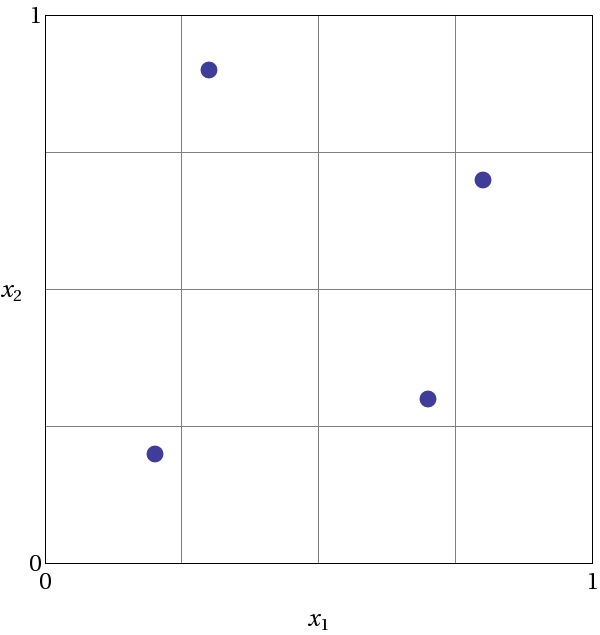
\includegraphics[scale=0.35]{images/lhs_graphic}
  \caption{An example of Latin hypercube sampling with four bins in
    design parameters $x_1$ and $x_2$. The dots
    are the sample sites.}
  \label{dace:figure01}
\end{figure}

The actual algorithm for generating Latin hypercube samples is more
complex than indicated by the description given above. For example,
the Latin hypercube sampling method implemented in the LHS
code~\cite{Swi04} takes into account a user-specified correlation
structure when selecting the sample sites. For more details on the
implementation of the LHS algorithm, see Reference~\cite{Swi04}.

\subsection{Uncertainty Quantification Example using Sampling Methods}\label{uq:uncertainty1}

The input file in Figure~\ref{uq:figure01} 
demonstrates the use of Latin hypercube Monte Carlo sampling for
assessing probability of failure as measured by specified response
levels.  The two-variable Textbook example problem (see
Equation~\ref{additional:textbook_f}) will be used to demonstrate
the application of sampling methods for uncertainty quantification
where it is assumed that $x_1$ and $x_2$ are uniform uncertain
variables on the interval $[0,1]$. 

The number of samples to
perform is controlled with the \texttt{samples} specification, the
type of sampling algorithm to use is controlled with the
\texttt{sample\_type} specification, the levels used for computing
statistics on the response functions is specified with the
\texttt{response\_levels} input, and the \texttt{seed} specification
controls the sequence of the pseudo-random numbers generated by the
sampling algorithms. The input samples generated are shown in
Figure~\ref{uq:figure02} for the case where \texttt{samples} = 5 and
\texttt{samples} = 10 for both \texttt{random} ($\circ$) and 
\texttt{lhs} ($+$) sample types.

\begin{figure}[htbp!]
  \centering \begin{bigbox} \begin{small}
  \verbatimtabinput[8]{textbook_uq_sampling.in} \end{small} \end{bigbox}
\caption{Dakota input file for UQ example using LHS --
see \texttt{Dakota/examples/users/textbook\_uq\_sampling.in} }
\label{uq:figure01}
\end{figure}

\begin{figure}[htbp!]
  \centering
  \subfigure{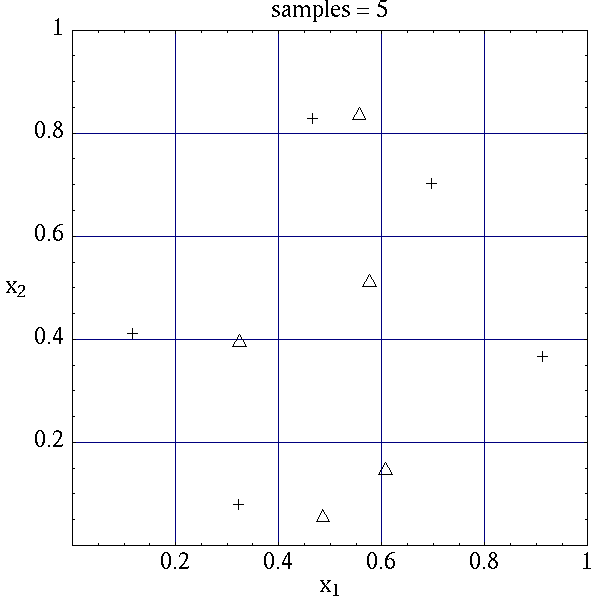
\includegraphics[scale=0.35]{images/input_samples5}}
  \subfigure{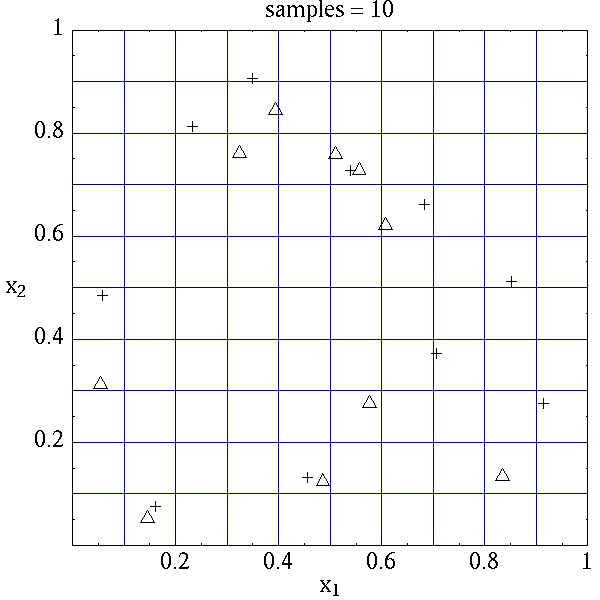
\includegraphics[scale=0.35]{images/input_samples10}}
  \caption{Distribution of input sample points for random ($\triangle$)
    and lhs ($+$) sampling for \texttt{samples=5} and \texttt{10}.}
  \label{uq:figure02}
\end{figure}

Latin hypercube sampling ensures full coverage of the range of the
input variables, which is often a problem with Monte Carlo sampling
when the number of samples is small. In the case of \texttt{samples =
5}, poor stratification is evident in $x_1$ as four out of the five
Monte Carlo samples are clustered in the range $0.35 < x_1 < 0.55$,
and the regions $x_1 < 0.3$ and $0.6 < x_1 < 0.9$ are completely
missed. For the case where \texttt{samples = 10}, some clustering in
the Monte Carlo samples is again evident with \texttt{4} samples in
the range $0.5 < x_1 < 0.55$. In both cases, the stratification with
LHS is superior. The response function statistics returned by Dakota
are shown in Figure~\ref{uq:figure03}. The first two blocks of output
specify the response sample means and sample standard deviations and
confidence intervals for these statistics, as well as coefficients of
variation. The last section of the output defines CDF pairs
(\texttt{distribution cumulative} was specified) for the response
functions by presenting the probability levels corresponding to the
specified response levels (\texttt{response\_levels} were set and the
default \texttt{compute probabilities} was used). Alternatively,
Dakota could have provided CCDF pairings, reliability levels
corresponding to prescribed response levels, or response levels
corresponding to prescribed probability or reliability levels.

\begin{figure}[htbp!]
\centering
\begin{bigbox}
\begin{small}
\begin{verbatim}
Statistics based on 10 samples:

Moments for each response function:
response_fn_1:  Mean = 3.83840e-01  Std. Dev. = 4.02815e-01
                Coeff. of Variation = 1.04944e+00
response_fn_2:  Mean = 7.47987e-02  Std. Dev. = 3.46861e-01
                Coeff. of Variation = 4.63726e+00
response_fn_3:  Mean = 7.09462e-02  Std. Dev. = 3.41532e-01
                Coeff. of Variation = 4.81397e+00

95% confidence intervals for each response function:
response_fn_1:  Mean = (  9.56831e-02, 6.71997e-01 ),
             Std Dev = (  2.77071e-01, 7.35384e-01 )
response_fn_2:  Mean = ( -1.73331e-01, 3.22928e-01 ),
             Std Dev = (  2.38583e-01, 6.33233e-01 )
response_fn_3:  Mean = ( -1.73371e-01, 3.15264e-01 ),
             Std Dev = (  2.34918e-01, 6.23505e-01 )

Probabilities for each response function:
Cumulative Distribution Function (CDF) for response_fn_1:
     Response Level  Probability Level  Reliability Index
     --------------  -----------------  -----------------
   1.0000000000e-01   3.0000000000e-01
   2.0000000000e-01   5.0000000000e-01
   6.0000000000e-01   7.0000000000e-01
Cumulative Distribution Function (CDF) for response_fn_2:
     Response Level  Probability Level  Reliability Index
     --------------  -----------------  -----------------
   1.0000000000e-01   5.0000000000e-01
   2.0000000000e-01   7.0000000000e-01
   6.0000000000e-01   9.0000000000e-01
Cumulative Distribution Function (CDF) for response_fn_3:
     Response Level  Probability Level  Reliability Index
     --------------  -----------------  -----------------
   1.0000000000e-01   6.0000000000e-01
   2.0000000000e-01   6.0000000000e-01
   6.0000000000e-01   9.0000000000e-01
\end{verbatim}
\end{small}
\end{bigbox}
\caption{Dakota response function statistics from UQ sampling example.}
\label{uq:figure03}
\end{figure}

In addition to obtaining statistical summary information of the type
shown in Figure~\ref{uq:figure03}, the results of LHS sampling also
include correlations. Four types of correlations are returned in the
output: simple and partial ``raw'' correlations, and simple and
partial ``rank'' correlations. The raw correlations refer to
correlations performed on the actual input and output data. Rank
correlations refer to correlations performed on the ranks of the data.
Ranks are obtained by replacing the actual data by the ranked values,
which are obtained by ordering the data in ascending order. For
example, the smallest value in a set of input samples would be given a
rank 1, the next smallest value a rank 2, etc. Rank correlations are
useful when some of the inputs and outputs differ greatly in
magnitude: then it is easier to compare if the smallest ranked input
sample is correlated with the smallest ranked output, for example.

Correlations are always calculated between two sets of sample data.
One can calculate correlation coefficients between two input
variables, between an input and an output variable (probably the most
useful), or between two output variables. The simple correlation
coefficients presented in the output tables are Pearson's correlation
coefficient, which is defined for two variables $x$ and $y$ as:
$\mathtt{Corr}(x,y) = \frac{\sum_{i}(x_{i}-\bar{x})(y_{i}-\bar{y})}
{\sqrt{\sum_{i}(x_{i}-\bar{x})^2\sum_{i}(y_{i}-\bar{y})^2}}$.
Partial correlation coefficients are similar to simple correlations,
but a partial correlation coefficient between two variables measures
their correlation while adjusting for the effects of the other
variables. For example, say one has a problem with two inputs and one
output; and the two inputs are highly correlated. Then the
correlation of the second input and the output may be very low after
accounting for the effect of the first input. The rank correlations
in Dakota are obtained using Spearman's rank correlation. Spearman's
rank is the same as the Pearson correlation coefficient except that it
is calculated on the rank data.

Figure~\ref{uq:figure04} shows an example of the correlation output
provided by Dakota for the input file in Figure~\ref{uq:figure01}.
Note that these correlations are presently only available when one
specifies \texttt{lhs} as the sampling method under \texttt{sampling}.
Also note that the simple and partial correlations should be similar in most
cases (in terms of values of correlation coefficients). This is
because we use a default ``restricted pairing'' method in the LHS
routine which forces near-zero correlation amongst uncorrelated
inputs.

\begin{figure}[htbp!]
\centering
\begin{bigbox}
\begin{small}
\begin{verbatim}
Simple Correlation Matrix between input and output:
                       x1           x2 response_fn_1 response_fn_2 response_fn_3
          x1  1.00000e+00
          x2 -7.22482e-02  1.00000e+00
response_fn_1 -7.04965e-01 -6.27351e-01  1.00000e+00
response_fn_2  8.61628e-01 -5.31298e-01 -2.60486e-01  1.00000e+00
response_fn_3 -5.83075e-01  8.33989e-01 -1.23374e-01 -8.92771e-01  1.00000e+00

Partial Correlation Matrix between input and output:
             response_fn_1 response_fn_2 response_fn_3
          x1 -9.65994e-01  9.74285e-01 -9.49997e-01
          x2 -9.58854e-01 -9.26578e-01  9.77252e-01

Simple Rank Correlation Matrix between input and output:
                       x1           x2 response_fn_1 response_fn_2 response_fn_3
          x1  1.00000e+00
          x2 -6.66667e-02  1.00000e+00
response_fn_1 -6.60606e-01 -5.27273e-01  1.00000e+00
response_fn_2  8.18182e-01 -6.00000e-01 -2.36364e-01  1.00000e+00
response_fn_3 -6.24242e-01  7.93939e-01 -5.45455e-02 -9.27273e-01  1.00000e+00

Partial Rank Correlation Matrix between input and output:
             response_fn_1 response_fn_2 response_fn_3
          x1 -8.20657e-01  9.74896e-01 -9.41760e-01
          x2 -7.62704e-01 -9.50799e-01  9.65145e-01
\end{verbatim}
\end{small}
\end{bigbox}
\caption{Correlation results using LHS Sampling.}
\label{uq:figure04}
\end{figure}

Finally, note that the LHS package can be used for design of
experiments over design and state variables by including an active
view override in the variables specification section of the Dakota
input file (see Section~\ref{variables:mixedview}). Then, instead of
iterating on only the uncertain variables, the LHS package will sample
over all of the active variables. In the \texttt{active all} view,
continuous design and continuous state variables are treated as having
uniform probability distributions within their upper and lower bounds,
discrete design and state variables are sampled uniformly from within
their sets or ranges, and any uncertain variables are sampled within
their specified probability distributions.

\subsection{Incremental Sampling}\label{uq:incremental}

In many situations, one may run an initial sample set and then need to
perform further sampling to get better estimates of the mean,
variance, and percentiles, and to obtain more comprehensive sample
coverage. We call this capability incremental sampling. Currently,
the LHS incremental sampling capability we have in Dakota requires that
the incremental samples are double the sample size of the previous
sample. That is, if one starts with a very small sample size of 10,
then one can use the incremental sampling capability to generate
sample sizes of 20, 40, 80, etc. Also, a Dakota restart file
(dakota.rst) must be available from the original sample. There are two
cases, random incremental and Latin Hypercube incremental sampling.
We assume that LHS incremental will be most frequently used. One
major advantage of LHS incremental sampling is that it maintains the
stratification and correlation structure of the original LHS sample.
That is, if one generated 2 independent LHS samples and just merged
them, the calculation of the accuracy of statistical measures such as
the mean and the variance would be slightly incorrect. However, in
the incremental case, the full sample (double the original size) is a
Latin Hypercube sample itself and statistical measures and their
accuracy can be properly calculated. The incremental sampling
capability is most useful when one is starting off with very small
samples. Once the sample size is more than a few hundred, the benefit
of incremental sampling diminishes.

\begin{enumerate}

\item Incremental Random Sampling. With incremental random sampling, 
the original sample set with N samples must be 
generated using \texttt{sample\_type} as \texttt{random}.
Then, the user can create a new Dakota input file that is very similar to the 
original one except the \texttt{sample\_type} should be defined to be 
\texttt{incremental\_random}. Random incremental sampling does not 
require a doubling of samples each time. Thus, the user 
can specify the number of samples (\texttt{samples}) to be a desired 
number (it can range from an additional one sample to a large integer), 
and the \texttt{previous\_samples} should be specified as N. For example, if
the first sample has 50 samples, and 10 more samples are desired, 
in the second Dakota run, the number
of samples should be set to 60 and the number of previous samples set
to 50. In this situation, only 10 new samples will be generated and
the final statistics will be reported on the full sample of 60. The
command line syntax for running the second sample is \texttt{dakota -i
input2.in -r dakota.rst} where input2.in is the input file with the
incremental sampling specification and dakota.rst is the restart file.
Note that if the restart file has a different name, that is fine; the
correct restart file name should be used.

\item Incremental Latin Hypercube Sampling. With incremental LHS sampling, 
the original sample set with N samples must be 
generated using \texttt{sample\_type} as \texttt{lhs}.
Then, the user can create a new Dakota input file that is very similar to the 
original one except the \texttt{sample\_type} should be defined to be 
\texttt{incremental\_lhs}, the number of samples (\texttt{samples}) should 
be 2N (twice the number of original samples), and
\texttt{previous\_samples} should be specified as N. For example, if
the first sample has 50 samples, in the second Dakota run, the number
of samples should be set to 100 and the number of previous samples set
to 50. In this situation, only 50 new samples will be generated and
the final statistics will be reported on the full sample of 100. The
command line syntax for running the second sample is \texttt{dakota -i
input2.in -r dakota.rst}, where input2.in is the input file with the
incremental sampling specification and dakota.rst is the restart file.
Note that if the restart file has a different name, that is fine; the
correct restart file name should be used.

\end{enumerate}

\section{Reliability Methods}\label{uq:reliability}

Reliability methods provide an alternative approach to uncertainty
quantification which can be less computationally demanding than
sampling techniques. Reliability methods for uncertainty
quantification are based on probabilistic approaches that compute
approximate response function distribution statistics based on
specified uncertain variable distributions. These response statistics
include response mean, response standard deviation, and cumulative or
complementary cumulative distribution functions (CDF/CCDF). These
methods are often more efficient at computing statistics in the tails
of the response distributions (events with low probability) than
sampling based approaches since the number of samples required to
resolve a low probability can be prohibitive.

The methods all answer the fundamental question: ``Given a set of
uncertain input variables, $\mathbf{X}$, and a scalar response
function, $g$, what is the probability that the response function is
below or above a certain level, $\bar{z}$?'' The former can be written
as $P[g(\mathbf{X}) \le \bar{z}] = \mathit{F}_{g}(\bar{z})$ where
$\mathit{F}_{g}(\bar{z})$ is the cumulative distribution function
(CDF) of the uncertain response $g(\mathbf{X})$ over a set of response
levels. The latter can be written as $P[g(\mathbf{X}) > \bar{z}]$ and
defines the complementary cumulative distribution function (CCDF).

This probability calculation involves a multi-dimensional integral
over an irregularly shaped domain of interest, $\mathbf{D}$, where
$g(\mathbf{X}) < z$ as displayed in Figure~\ref{uq:figure05} for the
case of two variables. The reliability methods all involve the
transformation of the user-specified uncertain variables,
$\mathbf{X}$, with probability density function, $p(x_1,x_2)$, which
can be non-normal and correlated, to a space of independent Gaussian
random variables, $\mathbf{u}$, possessing a mean value of zero and
unit variance (i.e., standard normal variables). The region of
interest, $\mathbf{D}$, is also mapped to the transformed space to
yield, $\mathbf{D_{u}}$ , where $g(\mathbf{U}) < z$ as shown in
Figure~\ref{uq:figure06}. The Nataf transformation~\cite{Der86},
which is identical to the Rosenblatt transformation~\cite{Ros52} in
the case of independent random variables, is used in Dakota to
accomplish this mapping. This transformation is performed to make the
probability calculation more tractable. In the transformed space,
probability contours are circular in nature as shown in
Figure~\ref{uq:figure06} unlike in the original uncertain variable
space, Figure~\ref{uq:figure05}. Also, the multi-dimensional integrals
can be approximated by simple functions of a single parameter,
$\beta$, called the reliability index. $\beta$ is the minimum
Euclidean distance from the origin in the transformed space to the
response surface. This point is also known as the most probable point
(MPP) of failure. Note, however, the methodology is equally applicable
for generic functions, not simply those corresponding to failure
criteria; this nomenclature is due to the origin of these methods
within the disciplines of structural safety and reliability.
Note that there are local and global reliability methods. The majority 
of the methods available are local, meaning that a local optimization 
formulation is used to locate one MPP. In contrast, global methods
can find multiple MPPs if they exist.
\begin{figure}[htbp!]
  \centering
  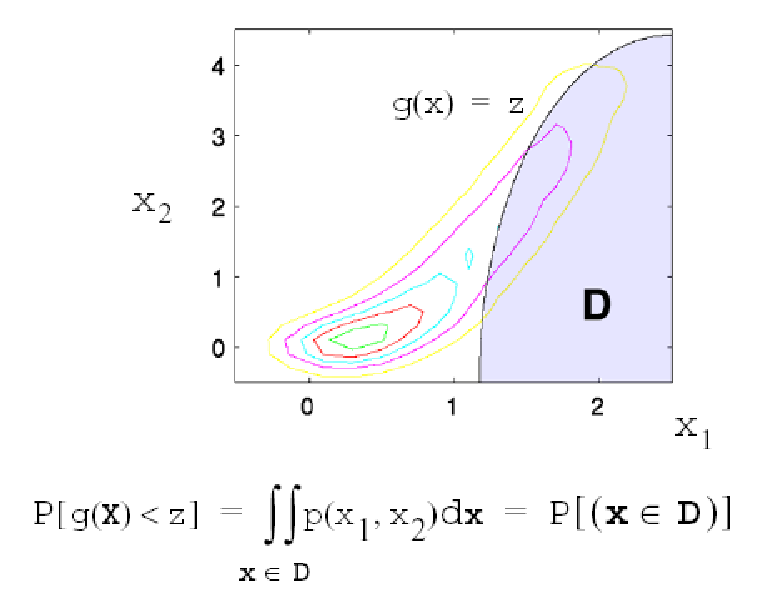
\includegraphics[scale=0.75]{images/cdf_orig_graphic}
  \caption{Graphical depiction of calculation of cumulative
    distribution function in the original uncertain variable space.}
  \label{uq:figure05}
\end{figure}

\begin{figure}[htbp!]
  \centering
  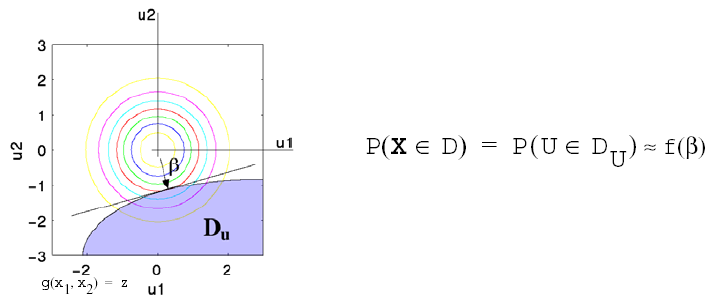
\includegraphics[scale=0.75]{images/cdf_tran_graphic}
  \caption{Graphical depiction of integration for the calculation of
    cumulative distribution function in the transformed uncertain
    variable space.}
  \label{uq:figure06}
\end{figure}

\subsection{Local Reliability Methods}\label{uq:reliability:local}

The Dakota Theory Manual~\cite{TheoMan} provides the algorithmic
details for the local reliability methods, including the Mean Value
method and the family of most probable point (MPP) search methods.


\subsubsection{Method mapping} \label{uq:reliability:local:map}

Given settings for limit state approximation, approximation order,
integration approach, and other details presented to this point, it is
evident that the number of algorithmic combinations is high.
Table~\ref{tab:rel_meth_map} provides a succinct mapping for some of
these combinations to common method names from the reliability
literature, where blue indicates the most well-known combinations and
gray indicates other supported combinations.
\begin{table}
\centering
\caption{Mapping from Dakota options to standard reliability methods.}
\label{tab:rel_meth_map}
\begin{tabular}{|c|c|c|}
\hline
& \multicolumn{2}{c|}{Order of approximation and integration} \\ \cline{2-3}
MPP search      & First order & Second order                        \\ \hline
none            & \cellcolor{blue}\textcolor{white}{MVFOSM}
                & \cellcolor[gray]{0.5}\textcolor{black}{MVSOSM}   \\ \hline
x\_taylor\_mean & \cellcolor{blue}\textcolor{white}{AMV}
                & \cellcolor[gray]{0.5}\textcolor{black}{AMV$^2$}  \\ \hline
u\_taylor\_mean & \cellcolor[gray]{0.5}\textcolor{black}{u-space AMV}
                & \cellcolor[gray]{0.5}\textcolor{black}{u-space AMV$^2$} \\
\hline
x\_taylor\_mpp  & \cellcolor{blue}\textcolor{white}{AMV+}
                & \cellcolor[gray]{0.5}\textcolor{black}{AMV$^2$+} \\ \hline
u\_taylor\_mpp  & \cellcolor[gray]{0.5}\textcolor{black}{u-space AMV+}
                & \cellcolor[gray]{0.5}\textcolor{black}{u-space AMV$^2$+} \\
\hline
x\_two\_point   & \cellcolor{blue}\textcolor{white}{TANA}
                & \cellcolor[gray]{0.5}                             \\ \hline
u\_two\_point   & \cellcolor[gray]{0.5}\textcolor{black}{u-space TANA}
                & \cellcolor[gray]{0.5}                             \\ \hline
no\_approx      & \cellcolor{blue}\textcolor{white}{FORM}
                & \cellcolor{blue}\textcolor{white}{SORM}           \\ \hline
\end{tabular}
\end{table}

Within the Dakota specification (refer to the Method Commands chapter
within the Reference Manual), the MPP search and integration order
selections are explicit in the method specification, but the order of
the approximation is inferred from the associated response
specification (as is done with local taylor series approximations
described in Section~\ref{models:surf:taylor}). Thus, reliability
methods do not have to be synchronized in approximation and
integration order as shown in the table; however, it is often
desirable to do so.


\subsection{Global Reliability Methods}\label{uq:reliability:global}

Global reliability methods are designed to handle nonsmooth and
multimodal failure surfaces, by creating global approximations based
on Gaussian process models. They accurately resolve a particular
contour of a response function and then estimate probabilities using
multimodal adaptive importance sampling.

The global reliability method in Dakota is called 
Efficient Global Reliability Analysis (EGRA) ~\cite{Bichon2008}. 
The name is due to its 
roots in efficient global optimization (EGO) ~\cite{Jon98,Hua06}.
The main idea in EGO-type optimization methods is that a global 
approximation is made of the underlying function. This approximation, 
which is a Gaussian process model, is used to guide the search by finding 
points which maximize the expected improvement function (EIF). 
The EIF is used to select the location at which a new training point should be
added to the Gaussian process model by maximizing the amount of improvement 
in the objective function that can be expected by adding that point.
A point could be expected to produce an improvement in the objective function 
if its predicted value is better than the current best solution, or if the 
uncertainty in its prediction is such that the probability of it producing
a better solution is high.
Because the uncertainty is higher in regions of the design space with fewer
observations, this provides a balance between exploiting areas of the
design space that predict good solutions, and exploring areas where more
information is needed.

The general procedure of these EGO-type methods is:
\begin{enumerate}
\item Build an initial Gaussian process model of the objective function.
%\item Use cross validation to ensure that the GP model is satisfactory.
\item Find the point that maximizes the EIF.
      If the EIF value at this point is sufficiently small, stop.
\item Evaluate the objective function at the point where the EIF is maximized.
      Update the Gaussian process model using this new point.
      Go to Step 2.
\end{enumerate}

Gaussian process (GP) models are used because
they provide not just a predicted value at an unsampled point, but also an
estimate of the prediction variance.
This variance gives an indication of the uncertainty in the GP model, which
results from the construction of the covariance function.
This function is based on the idea that when input points are near one another,
the correlation between their corresponding outputs will be high.
As a result, the uncertainty associated with the model's predictions will be
small for input points which are near the points used to train the model,
and will increase as one moves further from the training points.

The expected improvement function is used in EGO algorithms 
to select the location at which a new training point should be added.
The EIF is defined as the expectation that any point in the search
space will provide a better solution than the current best solution
based on the expected values and variances predicted by the GP model.
It is important to understand how the use of this EIF leads to optimal
solutions. The EIF indicates how much the objective function value at 
a new potential location 
is expected to be less than the predicted value at the current best solution.
Because the GP model provides a Gaussian distribution at each predicted
point, expectations can be calculated.
Points with good expected values and even a small variance will
have a significant expectation of producing a better solution (exploitation),
but so will points that have relatively poor expected values and greater
variance (exploration).
 
The application of EGO to reliability analysis, however, is made more
complicated due to the inclusion of equality constraints.
In forward reliability analysis, the response function appears as a 
constraint rather than the objective. That is, we want to satisfy 
the constraint that the response equals a threshold value 
and is on the limit state:  $G({\bf u})\!=\!\bar{z}$.
Therefore, the EIF function was modified to focus on feasibility, 
and instead of using an expected improvement function, we use an 
expected feasibility function (EFF) ~\cite{Bichon2008}. 
The EFF provides an indication of how well the response is expected 
to satisfy the equality constraint. 
Points where the expected value is close to the threshold
($\mu_G\!\approx\!\bar{z}$) and points with a large uncertainty in the
prediction will have large expected feasibility values.

The general outline of the EGRA algorithm is as follows:  LHS sampling 
is used to generate a small number of samples from the true response 
function. Then, an initial Gaussian process model is constructed. 
Based on the EFF, the point with maximum EFF is found using 
the global optimizer DIRECT. The true response function is then 
evaluated at this new point, and this point is added to the sample set 
and the process of building a new GP model and maximizing the EFF is 
repeated until the maximum EFF is small. At this stage, the GP model 
is accurate in the vicinity of the limit state. The GP model 
is then used to calculate the probability of failure 
using multimodal importance sampling, which is explained below. 

One method to calculate the probability of failure is 
to directly perform the probability 
integration numerically by sampling the response function.
Sampling methods can be 
prohibitively expensive because they generally require a large 
number of response function evaluations.
Importance sampling methods reduce this expense by focusing the samples in 
the important regions of the uncertain space.
They do this by centering the sampling density function at the MPP rather
than at the mean.
This ensures the samples will lie the region of interest, 
thus increasing the efficiency of the sampling method.
Adaptive importance sampling (AIS) further improves the efficiency by 
adaptively updating the sampling density function.
Multimodal adaptive importance sampling~\cite{Dey98} is a 
variation of AIS that allows for the use of multiple sampling densities 
making it better suited for cases where multiple sections of the limit state 
are highly probable.

Note that importance sampling methods require that the location of at least 
one MPP be known because it is used to center the initial sampling density.
However, current gradient-based, local search methods used in MPP search may 
fail to converge or may converge to poor solutions for 
highly nonlinear problems, possibly making these methods inapplicable.
The EGRA algorithm described above does 
not depend on the availability of accurate gradient information, making
convergence more reliable for nonsmooth response functions.
Moreover, EGRA has the ability to locate multiple failure points, which 
can provide multiple starting points and thus a good multimodal sampling density for the initial steps of multimodal AIS. The probability assessment 
using multimodal AIS thus incorporates probability of failure at 
multiple points.

\subsection{Uncertainty Quantification Examples using Reliability Analysis} \label{uq:reliability:ex}

%Reliability methods provide an alternative approach to uncertainty
%quantification which can be less computationally demanding than
%sampling techniques. 

In summary, the user can choose to perform either forward (RIA) or
inverse (PMA) mappings when performing a reliability analysis. With
either approach, there are a variety of methods from which to choose
in terms of limit state approximations (MVFOSM, MVSOSM, x-/u-space
AMV, x-/u-space AMV$^2$, x-/u-space AMV+, x-/u-space AMV$^2$+,
x-/u-space TANA, and FORM/SORM), probability integrations
(first-order or second-order), limit state Hessian selection
(analytic, finite difference, BFGS, or SR1), and MPP optimization
algorithm (SQP or NIP) selections.

All reliability methods output approximate values of the CDF/CCDF
response-probability-reliability levels for prescribed response levels
(RIA) or prescribed probability or reliability levels (PMA). In
addition, the MV methods additionally output estimates of the mean and
standard deviation of the response functions along with importance
factors for each of the uncertain variables in the case of independent
random variables.

\subsubsection{Mean-value Reliability with Textbook}
\label{uq:examples:mv}

Figure~\ref{uq:examples:mv_input} shows the Dakota input file for an
example problem that demonstrates the simplest reliability method,
called the mean value method (also referred to as the Mean Value First
Order Second Moment method). It is specified with method keyword
\texttt{local\_reliability}. This method calculates the mean and
variance of the response function based on information about the mean
and variance of the inputs and gradient information at the mean of the
inputs. The mean value method is extremely cheap computationally (only
five runs were required for the textbook function), but can be quite
inaccurate, especially for nonlinear problems and/or problems with
uncertain inputs that are significantly non-normal. More detail on the
mean value method can be found in the Local Reliability Methods
section of the Dakota Theory Manual~\cite{TheoMan}, and more detail on
reliability methods in general (including the more advanced methods)
is found in Section~\ref{uq:reliability}.

Example output from the mean value method is displayed in 
Figure~\ref{uq:examples:mv_results}. Note that since the mean of both inputs
is 1, the mean value of the output for response 1 is zero. 
However, the mean values of the constraints are both 0.5. 
The mean value results indicate that variable x1 is more 
important in constraint 1 while x2 is more important in constraint 2, 
which is the case based on Equation~\ref{additional:textbook_f}.

\begin{figure}[htbp!]
  \centering
  \begin{bigbox}
    \begin{small}
      \verbatimtabinput[8]{textbook_uq_meanvalue.in}
    \end{small}
  \end{bigbox}
  \caption{Mean Value Reliability Method: the Dakota input file --
see \texttt{Dakota/examples/users/textbook\_uq\_meanvalue.in} }
  \label{uq:examples:mv_input}
\end{figure}

\begin{figure}[htbp!]
\centering
\begin{bigbox}
\begin{small}
\begin{verbatim}
-----------------------------------------------------------------
MV Statistics for response_fn_1:
  Approximate Mean Response                  =  0.0000000000e+00
  Approximate Standard Deviation of Response =  0.0000000000e+00
  Importance Factors not available.
MV Statistics for response_fn_2:
  Approximate Mean Response                  =  5.0000000000e-01
  Approximate Standard Deviation of Response =  1.0307764064e+00
  Importance Factor for variable TF1ln       =  9.4117647059e-01
  Importance Factor for variable TF2ln       =  5.8823529412e-02
MV Statistics for response_fn_3:
  Approximate Mean Response                  =  5.0000000000e-01
  Approximate Standard Deviation of Response =  1.0307764064e+00
  Importance Factor for variable TF1ln       =  5.8823529412e-02
  Importance Factor for variable TF2ln       =  9.4117647059e-01
-----------------------------------------------------------------
\end{verbatim}
\end{small}
\end{bigbox}
\caption{Results of the Mean Value Method on the Textbook Function}
\label{uq:examples:mv_results}
\end{figure}

\subsubsection{FORM Reliability with Lognormal Ratio}

This example quantifies the uncertainty in the ``log ratio'' response
function:
\begin{equation}
g(x_1,x_2) = \frac{x_1}{x_2}
\end{equation}
by computing approximate response statistics using reliability
analysis to determine the response cumulative distribution function:
\begin{equation}
P[g(x_1,x_2) < \bar{z}]
\end{equation}
where $X_1$ and $X_2$ are identically distributed lognormal random
variables with means of \texttt{1}, standard deviations of
\texttt{0.5}, and correlation coefficient of \texttt{0.3}.

A Dakota input file showing RIA using FORM (option 7 in limit state
approximations combined with first-order integration) is listed in
Figure~\ref{uq:rel_input_form}.
The user first specifies the \texttt{local\_reliability}
method, followed by the MPP search approach and integration order. In
this example, we specify \texttt{mpp\_search no\_approx} and utilize
the default first-order integration to select FORM. Finally, the user
specifies response levels or probability/reliability levels to
determine if the problem will be solved using an RIA approach or a PMA
approach. In the example figure of~\ref{uq:rel_input_form}, we use
RIA by specifying a range of \texttt{response\_levels} for the
problem. The resulting output for this input is shown in
Figure~\ref{uq:rel_output_form}, with probability and reliability
levels listed for each response level. Figure~\ref{uq:rel_form_compare} 
shows that FORM compares favorably to an exact analytic solution for
this problem. Also note that FORM does have some error in the
calculation of CDF values for this problem, but it is a very small
error (on the order of e-11), much smaller than the error obtained
when using a Mean Value method, which will be discussed next.
\begin{figure}[htbp!]
  \centering
  \begin{bigbox}
    \begin{small}
      \verbatimtabinput[8]{logratio_uq_reliability.in}
    \end{small}
  \end{bigbox}
\caption{Dakota input file for Reliability UQ example using FORM --
see \texttt{Dakota/examples/users/logratio\_uq\_reliability.in} }
\label{uq:rel_input_form}
\end{figure}

\begin{figure}[htbp!]
\centering
\begin{bigbox}
\begin{small}
\begin{verbatim}
Cumulative Distribution Function (CDF) for response_fn_1:
     Response Level  Probability Level  Reliability Index
     --------------  -----------------  -----------------
   4.0000000000e-01   4.7624085962e-02   1.6683404020e+00
   5.0000000000e-01   1.0346525475e-01   1.2620507942e+00
   5.5000000000e-01   1.3818404972e-01   1.0885143628e+00
   6.0000000000e-01   1.7616275822e-01   9.3008801339e-01
   6.5000000000e-01   2.1641741368e-01   7.8434989943e-01
   7.0000000000e-01   2.5803428381e-01   6.4941748143e-01
   7.5000000000e-01   3.0020938124e-01   5.2379840558e-01
   8.0000000000e-01   3.4226491013e-01   4.0628960782e-01
   8.5000000000e-01   3.8365052982e-01   2.9590705956e-01
   9.0000000000e-01   4.2393548232e-01   1.9183562480e-01
   1.0000000000e+00   5.0000000000e-01   6.8682233460e-12
   1.0500000000e+00   5.3539344228e-01  -8.8834907167e-02
   1.1500000000e+00   6.0043460094e-01  -2.5447217462e-01
   1.2000000000e+00   6.3004131827e-01  -3.3196278078e-01
   1.2500000000e+00   6.5773508987e-01  -4.0628960782e-01
   1.3000000000e+00   6.8356844630e-01  -4.7770089473e-01
   1.3500000000e+00   7.0761025532e-01  -5.4641676380e-01
   1.4000000000e+00   7.2994058691e-01  -6.1263331274e-01
   1.5000000000e+00   7.6981945355e-01  -7.3825238860e-01
   1.5500000000e+00   7.8755158269e-01  -7.9795460350e-01
   1.6000000000e+00   8.0393505584e-01  -8.5576118635e-01
   1.6500000000e+00   8.1906005158e-01  -9.1178881995e-01
   1.7000000000e+00   8.3301386860e-01  -9.6614373461e-01
   1.7500000000e+00   8.4588021938e-01  -1.0189229206e+00
\end{verbatim}
\end{small}
\end{bigbox}
\caption{Output from Reliability UQ example using FORM.}
\label{uq:rel_output_form}
\end{figure}

\begin{figure}[htbp!]
  \centering
  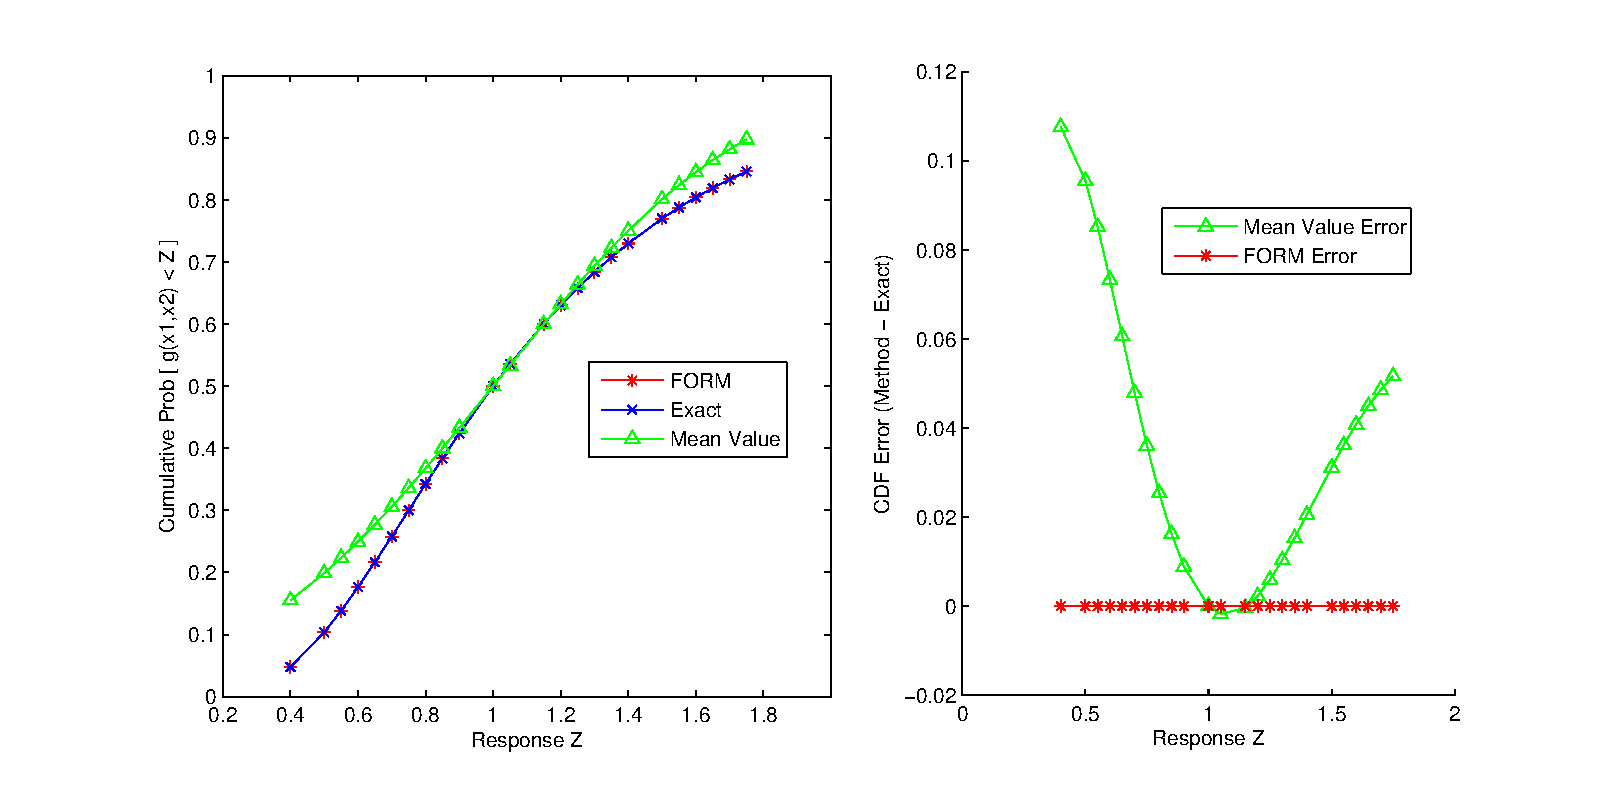
\includegraphics[scale=0.5]{images/cdf_form}
\caption{Comparison of the cumulative distribution function (CDF) computed by
FORM, the Mean Value method, and the exact CDF for $g(x_1,x_2)=\frac{x_1}{x_2}$}
\label{uq:rel_form_compare}
\end{figure}

If the user specifies \texttt{local\_reliability} as a method with no
additional specification on how to do the MPP search, then no MPP
search is done: the Mean Value method is used. The MV results are
shown in Figure~\ref{uq:rel_output_mv} and consist of approximate mean
and standard deviation of the response, the importance factors for
each uncertain variable, and approximate probability/reliability
levels for the prescribed response levels that have been inferred from
the approximate mean and standard deviation (see Mean Value section in
Reliability Methods Chapter of Dakota Theory
Manual~\cite{TheoMan}). It is evident that the statistics are
considerably different from the fully converged FORM results; however,
these rough approximations are also much less expensive to
calculate. The importance factors are a measure of the sensitivity of
the response function(s) to the uncertain input variables, but in this
case, are not separable due to the presence of input correlation
coefficients. A comparison of the mean value results with the FORM
results is shown in Figure~\ref{uq:rel_form_compare}. The mean value
results are not accurate near the tail values of the CDF, and can
differ from the exact solution by as much as 0.11 in CDF estimates. A
comprehensive comparison of various reliability methods applied to the
logratio problem is provided in ~\cite{Eld06a}.

\begin{figure}[htbp!] % Imp factors only if uncorrelated
\begin{bigbox}
\begin{small}
\begin{verbatim}
MV Statistics for response_fn_1:
  Approximate Mean Response                  =  1.0000000000e+00
  Approximate Standard Deviation of Response =  5.9160798127e-01
  Importance Factors not available.
Cumulative Distribution Function (CDF) for response_fn_1:
     Response Level  Probability Level  Reliability Index
     --------------  -----------------  -----------------
   4.0000000000e-01   1.5524721837e-01   1.0141851006e+00
   5.0000000000e-01   1.9901236093e-01   8.4515425050e-01
   5.5000000000e-01   2.2343641149e-01   7.6063882545e-01
   6.0000000000e-01   2.4948115037e-01   6.7612340040e-01
   6.5000000000e-01   2.7705656603e-01   5.9160797535e-01
   7.0000000000e-01   3.0604494093e-01   5.0709255030e-01
   7.5000000000e-01   3.3630190949e-01   4.2257712525e-01
   8.0000000000e-01   3.6765834596e-01   3.3806170020e-01
   8.5000000000e-01   3.9992305332e-01   2.5354627515e-01
   9.0000000000e-01   4.3288618783e-01   1.6903085010e-01
   1.0000000000e+00   5.0000000000e-01   0.0000000000e+00
   1.0500000000e+00   5.3367668035e-01  -8.4515425050e-02
   1.1500000000e+00   6.0007694668e-01  -2.5354627515e-01
   1.2000000000e+00   6.3234165404e-01  -3.3806170020e-01
   1.2500000000e+00   6.6369809051e-01  -4.2257712525e-01
   1.3000000000e+00   6.9395505907e-01  -5.0709255030e-01
   1.3500000000e+00   7.2294343397e-01  -5.9160797535e-01
   1.4000000000e+00   7.5051884963e-01  -6.7612340040e-01
   1.5000000000e+00   8.0098763907e-01  -8.4515425050e-01
   1.5500000000e+00   8.2372893005e-01  -9.2966967555e-01
   1.6000000000e+00   8.4475278163e-01  -1.0141851006e+00
   1.6500000000e+00   8.6405064339e-01  -1.0987005257e+00
   1.7000000000e+00   8.8163821351e-01  -1.1832159507e+00
   1.7500000000e+00   8.9755305196e-01  -1.2677313758e+00
\end{verbatim}
\end{small}
\end{bigbox}
\caption{Output from Reliability UQ example using MV.}
\label{uq:rel_output_mv}
\end{figure}

Additional reliability analysis and design results are provided in 
Sections~\ref{additional:logratio}-\ref{additional:steel_column}.


\section{Stochastic Expansion Methods}\label{uq:expansion}


%The objective of these techniques is to characterize the response of
%systems whose governing equations involve stochastic coefficients. 
The development of these techniques mirrors that of deterministic
finite element analysis through the utilization of the concepts of
projection, orthogonality, and weak convergence. The polynomial chaos
expansion is based on a multidimensional orthogonal polynomial
approximation and the stochastic collocation approach is based on a
multidimensional interpolation polynomial approximation, both formed
in terms of standardized random variables. A distinguishing feature of
these two methodologies is that the final solution is expressed as a
functional mapping, and not merely as a set of statistics as is the
case for many nondeterministic methodologies.  This makes these
techniques particularly attractive for use in multi-physics
applications which link different analysis packages.  The first
stochastic expansion method is the polynomial chaos expansion
(PCE)~\cite{Gha99,Gha91}. For smooth functions (i.e.,
analytic, infinitely-differentiable) in $L^2$ (i.e., possessing finite
variance), exponential convergence rates can be obtained under order
refinement for integrated statistical quantities of interest such as
mean, variance, and probability. Dakota implements the generalized
PCE approach using the Wiener-Askey
scheme~\cite{XiuKarn02}, in which Hermite, Legendre, Laguerre, Jacobi,
and generalized Laguerre orthogonal polynomials are used for modeling
the effect of continuous random variables described by normal,
uniform, exponential, beta, and gamma probability distributions,
respectively\footnote{Orthogonal polynomial selections also exist for
  discrete probability distributions, but are not yet supported in
  Dakota.}. These orthogonal polynomial selections are optimal for
these distribution types since the inner product weighting function
corresponds\footnote{Identical support range; weight differs by at
  most a constant factor.} to the probability density functions for
these continuous distributions. Orthogonal polynomials can be computed
for any positive weight function, so these five classical orthogonal
polynomials may be augmented with numerically-generated polynomials
for other probability distributions (e.g., for lognormal, extreme
value, and histogram distributions).  When independent standard random
variables are used (or computed through transformation), the variable
expansions are uncoupled, allowing the polynomial orthogonality
properties to be applied on a per-dimension basis. This allows one to
mix and match the polynomial basis used for each variable without
interference with the spectral projection scheme for the response.

In non-intrusive PCE, simulations are used as black boxes and the
calculation of chaos expansion coefficients for response metrics of
interest is based on a set of simulation response evaluations. To
calculate these response PCE coefficients, two primary classes of
approaches have been proposed: spectral projection and regression. The
spectral projection approach projects the response against each basis
function using inner products and employs the polynomial orthogonality
properties to extract each coefficient. Each inner product involves a
multidimensional integral over the support range of the weighting
function, which can be evaluated numerically using sampling,
tensor-product quadrature, Smolyak sparse grid~\cite{Smolyak_63}, or
cubature~\cite{stroud} approaches. The regression approach finds a set
of PCE coefficients which best match a set of response values obtained
from either a design of computer experiments (``point
collocation''~\cite{pt_colloc1}) or from a randomly selected subset of
tensor Gauss points (``probabilistic
collocation''~\cite{Tat95}). Various methods can be used to solve the
resulting linear system, including least squares methods for
over-determined systems and compressed sensing methods for
under-determined systems. Details of these methods are documented in
the Linear regression section of the Dakota Theory
Manual~\cite{TheoMan} and the necessary specifications needed to
activate these techniques are listed in the Methods chapter of the
Dakota Reference Manual~\cite{RefMan}.

Stochastic collocation (SC) is another stochastic expansion technique
for UQ that is closely related to PCE. As for PCE, exponential
convergence rates can be obtained under order refinement for
integrated statistical quantities of interest, provided that the
response functions are smooth with finite variance. The primary
distinction is that, whereas PCE estimates coefficients for known
multivariate orthogonal polynomial basis functions, SC forms
multivariate interpolation polynomial bases for known coefficients.
The interpolation polynomials may be either local or global and either
value-based or gradient-enhanced (four combinations: Lagrange,
Hermite, piecewise linear spline, and piecewise cubic spline), and may
be used within nodal or hierarchical interpolation
formulations. Interpolation is performed on structured grids such as
tensor-product or sparse grids. Starting from a tensor-product
multidimensional interpolation polynomial in the value-based case
(Lagrange or piecewise linear spline), we have the feature that the
$i^{th}$ interpolation polynomial has a value of 1 at collocation
point $i$ and a value of 0 for all other collocation points, leading
to the use of expansion coefficients that are just the response values
at each of the collocation points. In the gradient-enhanced case
(Hermite or piecewise cubic spline), SC includes both type 1 and type
2 interpolation polynomials, where the former interpolate the values
while producing zero gradients and the latter interpolate the
gradients while producing zero values (refer to~\cite{TheoMan} for
additional details). Sparse interpolants are weighted sums of these
tensor interpolants;
%and retain the use of response values as expansion coefficients;
however, they are only interpolatory for sparse grids based on fully 
nested rules and will exhibit some interpolation error at the 
collocation points for sparse grids based on non-nested rules.
A key to maximizing performance with SC is performing collocation
using the Gauss points and weights from the same optimal orthogonal
polynomials used in PCE. 
For use of standard Gauss integration rules (not nested variants such
as Gauss-Patterson or Genz-Keister) within tensor-product quadrature,
tensor PCE expansions and tensor SC interpolants are equivalent in
that identical polynomial approximations are
generated~\cite{ConstTPQ}. Moreover, this equivalence can be extended
to sparse grids based on standard Gauss rules, provided that a sparse
PCE is formed based on a weighted sum of tensor expansions~\cite{ConstSSG}.

The Dakota Theory Manual~\cite{TheoMan} provides full algorithmic
details for the PCE and SC methods.


\subsection{Uncertainty Quantification Examples using Stochastic Expansions} \label{uq:stoch_exp:ex}

\subsubsection{Polynomial Chaos Expansion for Rosenbrock}
\label{uq:stoch_exp:ex:pce}

%The term ``Polynomial Chaos'' refers to the representation of a stochastic 
%process as a polynomial expansion in random (or stochastic) variables. This 
%representation acts as a response surface that maps stochastic inputs to 
%stochastic outputs. Desired statistics can then be obtained from the 
%response surface either analytically or by re-sampling the fast surrogate.
%Additional details regarding the method are provided in

A typical Dakota input file for performing an uncertainty
quantification using PCE is shown in
Figure~\ref{uq:examples:pce_input}.  In this example, we compute CDF
probabilities for six response levels of Rosenbrock's function. Since
Rosenbrock is a fourth order polynomial and we employ a fourth-order
expansion using an optimal basis (Legendre for uniform random
variables), we can readily obtain a polynomial expansion which exactly
matches the Rosenbrock function. In this example, we select Gaussian
quadratures using an anisotropic approach (fifth-order quadrature in
$x_1$ and third-order quadrature in $x_2$), resulting in a total of 15
function evaluations to compute the PCE coefficients.

\begin{figure}[htbp!]
  \centering
  \begin{bigbox}
    \begin{small}
      \verbatimtabinput[8]{rosen_uq_pce.in}
    \end{small}
  \end{bigbox}
\caption{Dakota input file for performing UQ using polynomial chaos expansions --
see \texttt{Dakota/examples/users/rosen\_uq\_pce.in} }
\label{uq:examples:pce_input}
\end{figure}

The tensor product quadature points upon which the expansion is calculated 
are shown in Figure~\ref{uq:examples:rosen_pce_points}. 
The tensor product generates
all combinations of values from each individual dimension: it is an 
all-way pairing of points.

\begin{figure}[htbp!]
  \centering
  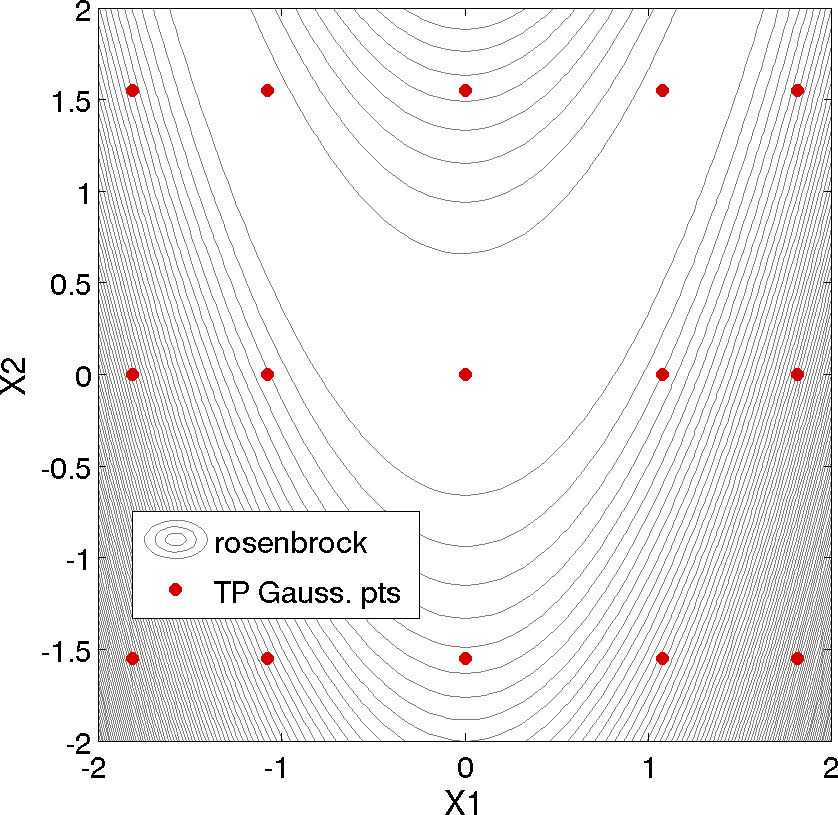
\includegraphics[height=2.5in]{images/rosen_pce_pts}
  \caption{Rosenbrock polynomial chaos example: tensor product quadrature points.}
  \label{uq:examples:rosen_pce_points}
\end{figure}

Once the expansion coefficients have been calculated, some statistics
are available analytically and others must be evaluated numerically.
For the numerical portion, the input file specifies the use of 10000
samples, which will be evaluated on the expansion to compute the CDF
probabilities. In Figure~\ref{uq:examples:pce_out}, excerpts from the
results summary are presented, where we first see a summary of the PCE
coefficients which exactly reproduce Rosenbrock for a Legendre
polynomial basis. The analytic statistics for mean, standard
deviation, and COV are then presented. For example, the mean is 455.66
and the standard deviation is 606.56. The moments are followed by
global sensitivity indices (Sobol' indices).This example shows that
variable x1 has the largest main effect (0.497) as compared with
variable x2 (0.296) or the interaction between x1 and x2 (0.206).
After the global sensitivity indices, the local sensitivities are
presented, evaluated at the mean values.  Finally, we see the
numerical results for the CDF probabilities based on 10000 samples
performed on the expansion. For example, the probability that the
Rosenbrock function is less than 100 over these two uncertain
variables is 0.342. Note that this is a very similar estimate to what
was obtained using 200 Monte Carlo samples, with fewer true function
evaluations.
\begin{figure}[htbp!]
\centering
\begin{bigbox}
%\begin{footnotesize}
\begin{scriptsize}
\begin{verbatim}
Polynomial Chaos coefficients for response_fn_1:
        coefficient   u1   u2
        ----------- ---- ----
   4.5566666667e+02   P0   P0
  -4.0000000000e+00   P1   P0
   9.1695238095e+02   P2   P0
  -9.9475983006e-14   P3   P0
   3.6571428571e+02   P4   P0
  -5.3333333333e+02   P0   P1
  -3.9968028887e-14   P1   P1
  -1.0666666667e+03   P2   P1
  -3.3573144265e-13   P3   P1
   1.2829737273e-12   P4   P1
   2.6666666667e+02   P0   P2
   2.2648549702e-13   P1   P2
   4.8849813084e-13   P2   P2
   2.8754776338e-13   P3   P2
  -2.8477220582e-13   P4   P2
-------------------------------------------------------------------
Statistics derived analytically from polynomial expansion:

Moment-based statistics for each response function:
                            Mean           Std Dev          Skewness          Kurtosis
response_fn_1
  expansion:    4.5566666667e+02  6.0656024184e+02
  numerical:    4.5566666667e+02  6.0656024184e+02  1.9633285271e+00  3.3633861456e+00

Covariance among response functions:
[[  3.6791532698e+05 ]] 

Local sensitivities for each response function evaluated at uncertain variable means:
response_fn_1:
 [ -2.0000000000e+00  2.4055757386e-13 ] 

Global sensitivity indices for each response function:
response_fn_1 Sobol indices:
                                  Main             Total
                      4.9746891383e-01  7.0363551328e-01 x1
                      2.9636448672e-01  5.0253108617e-01 x2
                           Interaction
                      2.0616659946e-01 x1 x2 

Statistics based on 10000 samples performed on polynomial expansion:

Probability Density Function (PDF) histograms for each response function:
PDF for response_fn_1:
          Bin Lower          Bin Upper      Density Value
          ---------          ---------      -------------
   6.8311107124e-03   1.0000000000e-01   2.0393073423e-02
   1.0000000000e-01   1.0000000000e+00   1.3000000000e-02
   1.0000000000e+00   5.0000000000e+01   4.7000000000e-03
   5.0000000000e+01   1.0000000000e+02   1.9680000000e-03
   1.0000000000e+02   5.0000000000e+02   9.2150000000e-04
   5.0000000000e+02   1.0000000000e+03   2.8300000000e-04
   1.0000000000e+03   3.5755437782e+03   5.7308286215e-05

Level mappings for each response function:
Cumulative Distribution Function (CDF) for response_fn_1:
     Response Level  Probability Level  Reliability Index  General Rel Index
     --------------  -----------------  -----------------  -----------------
   1.0000000000e-01   1.9000000000e-03
   1.0000000000e+00   1.3600000000e-02
   5.0000000000e+01   2.4390000000e-01
   1.0000000000e+02   3.4230000000e-01
   5.0000000000e+02   7.1090000000e-01
   1.0000000000e+03   8.5240000000e-01
-------------------------------------------------------------------
\end{verbatim}
\end{scriptsize}
%\end{footnotesize}
\end{bigbox}
\caption{Excerpt of UQ output for polynomial chaos example.}
\label{uq:examples:pce_out}
\end{figure}

\subsubsection{Uncertainty Quantification Example using Stochastic Collocation}
\label{uq:stoch_exp:ex:sc}

%A typical Dakota input file for performing an uncertainty
%quantification using polynomial chaos expansions is shown in
%Section~\ref{uq:stoch_exp:ex:pce}, which illustrates PCE defined from an
%anisotropic tensor-product quadrature grid. The uncertain variables
%are uniforms, so the expansion is built using classical Legendre
%polynomials. 

Compared to the previous PCE example, this section presents a more
sophisticated example, where we use stochastic collocation built on an
anisotropic sparse grid defined from numerically-generated orthogonal
polynomials. The uncertain variables are lognormal in this example and
the orthogonal polynomials are generated from Gauss-Wigert recursion
coefficients~\cite{simpson_gw} in combination with the Golub-Welsch
procedure~\cite{GolubWelsch69}.  The input file is shown in
Figure~\ref{uq:figure11}.  Note that the dimension preference of
$(2,1)$ is inverted to define a $\gamma$ weighting vector of $(0.5,1)$
(and $\underline{\gamma}$ of $0.5$) for use in the anisotropic Smolyak
index set constraint (see Smolyak sparse grids section in Stochastic
Expansion Methods chapter in Dakota Theory Manual~\cite{TheoMan}). In
this example, we compute CDF probabilities for six response levels of
Rosenbrock's function. This example requires 19 function evaluations
to calculate the interpolating polynomials in stochastic collocation
and the resulting expansion exactly reproduces Rosenbrock's function.
The placement of the points generated by the sparse grid is shown in
Figure~\ref{uq:figure11b}.

\begin{figure}[htbp!]
  \centering
  \begin{bigbox}
    \begin{small}
      \verbatimtabinput[8]{rosen_uq_sc.in}
    \end{small}
  \end{bigbox}
\caption{Dakota input file for performing UQ using stochastic collocation --
see \texttt{Dakota/examples/users/rosen\_uq\_sc.in} }
\label{uq:figure11}
\end{figure}

\begin{figure}[htbp!]
  \centering
  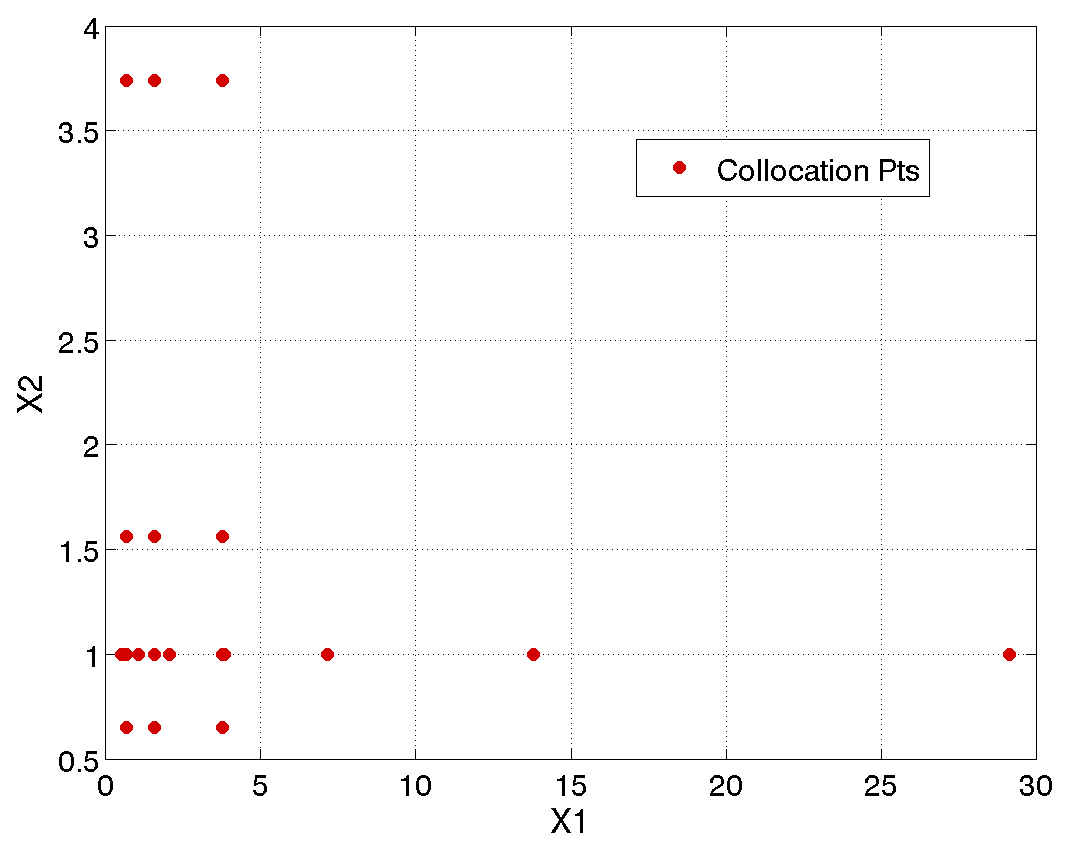
\includegraphics[height=2.5in]{images/rosen_sc_pts}
  \caption{Rosenbrock stochastic collocation example: sparse grid points.}
  \label{uq:figure11b}
\end{figure}

Once the expansion coefficients have been calculated, some statistics
are available analytically and others must be evaluated numerically.
For the numerical portion, the input file specifies the use of 10000
samples, which will be evaluated on the expansion to compute the CDF
probabilities. In Figure~\ref{uq:figure12}, excerpts from the results
summary are presented. We first see the moment statistics for mean,
standard deviation, skewness, and kurtosis computed by numerical
integration (see Analytic moments section in Stochastic Expansion
Methods chapter in Dakota Theory Manual~\cite{TheoMan}), where the
numerical row corresponds to integration using the original response
values and the expansion row corresponds to integration using values
from the interpolant. The response covariance (collapsing to a single
variance value for one response function) and global sensitivity
indices (Sobol' indices) are presented next. This example shows that
variable x1 has the largest main effect (0.99) as compared with
variable x2 (0.0007) or the interaction between x1 and x2 (0.005).
%After the global sensitivity indices, the local, analytic random 
%variable sensitivities are presented, as computed from
%Eqs.~\ref{eq:dR_dx}-\ref{eq:dR_dxi_sc}, evaluated at the mean values.
Finally, we see the numerical results for the CDF probabilities based
on 10000 samples performed on the expansion. For example, the probability 
that the Rosenbrock function is less than 100 is 0.7233. Note that these 
results are significantly different than the ones presented in 
Section~\ref{uq:stoch_exp:ex:pce} because of 
the different assumptions about the inputs: uniform[-2,2] versus
lognormals with means of 1.0 and standard deviations of 0.5. 
\begin{figure}[htbp!]
\centering
\begin{bigbox}
\begin{footnotesize}
\begin{verbatim}
Statistics derived analytically from polynomial expansion:

Moment-based statistics for each response function:
                            Mean           Std Dev          Skewness          Kurtosis
response_fn_1
  expansion:    2.5671972656e+02  2.0484189184e+03  2.7419241630e+02  1.9594567379e+06
  numerical:    2.5671972656e+02  2.0484189184e+03  2.7419241630e+02  1.9594567379e+06

Covariance among response functions:
[[  4.1960200651e+06 ]] 

Global sensitivity indices for each response function:
response_fn_1 Sobol indices:
                                  Main             Total
                      9.9391978710e-01  9.9928724777e-01 x1
                      7.1275222945e-04  6.0802128961e-03 x2
                           Interaction
                      5.3674606667e-03 x1 x2 

Statistics based on 10000 samples performed on polynomial expansion:

Level mappings for each response function:
Cumulative Distribution Function (CDF) for response_fn_1:
     Response Level  Probability Level  Reliability Index  General Rel Index
     --------------  -----------------  -----------------  -----------------
   1.0000000000e-01   1.8100000000e-02
   1.0000000000e+00   8.7800000000e-02
   5.0000000000e+01   5.8410000000e-01
   1.0000000000e+02   7.2330000000e-01
   5.0000000000e+02   9.2010000000e-01
   1.0000000000e+03   9.5660000000e-01
\end{verbatim}
\end{footnotesize}
\end{bigbox}
\caption{Excerpt of UQ output for stochastic collocation example.}
\label{uq:figure12}
\end{figure}

\section{Importance Sampling Methods}\label{uq:importance}

Importance sampling is a method that allows one to estimate statistical
quantities such as failure probabilities (e.g. the probability that
a response quantity will exceed a threshold or fall below a threshold value)
in a way that is more efficient than Monte Carlo sampling. The core idea
in importance sampling is that one generates samples that preferentially
samples important regions in the space (e.g. in or near the failure region
or user-defined region of interest), and then appropriately weights
the samples to obtain an unbiased estimate of the failure probability
~\cite{Srinivasan2002}.
In importance sampling, the samples are generated from a density which is
called the importance density:  it is not the original probability density
of the input distributions. The importance density should be centered near the
failure region of interest. For black-box simulations such as those commonly
interfaced with Dakota, it is difficult to specify the importance density a priori:
the user often does not know where the failure region lies, especially in a high-dimensional
space.~\cite{Swiler2010}

More formally, we define the objective of importance sampling as calculating the probability, $P$, that the output will exceed a threshold level. This is a failure 
probability, where the failure probability is defined as some scalar function, 
$y\left(\textbf{X}\right)$, exceeding a threshold, $T$, 
where the inputs, $\textbf{X}$, are randomly distributed with density, $\rho\left(\textbf{X}\right)$. 
When evaluating $y\left(\textbf{X}\right)$ is sufficiently expensive or $P$ is sufficiently small, Monte Carlo (MC) sampling methods to estimate $P$ will be infeasible due to the large number of function evaluations required
for a specified accuracy. 

The probability of failure can be thought of as the mean rate of occurrence
of failure. The Monte Carlo (MC) estimate of $P$ is therefore the sample
mean of the indicator function, $I\left(\textbf{X}\right)$,
\begin{equation}
P_{MC}=\frac{1}{N}\sum_{i=1}^{N}I\left(\mathbf{X_i}\right)\ \ \textbf{X}\sim \rho\left(\textbf{X}\right),
\label{mc_ind}
\end{equation}
where $N$ samples, $\mathbf{X_i}$, are drawn from
$\rho\left(\textbf{X}\right)$,
and the indicator function $I\left(\textbf{X}\right)$
is 1 if failure occurs and zero otherwise.

Importance sampling draws samples from the importance density 
$\rho'\left(\textbf{X}\right)$ and scales the sample mean by the importance density:
\begin{equation}
P_{IS}=\frac{1}{N}\sum_{i=1}^N \left(I\left(\mathbf{X_i}\right)\frac{\rho\left(\mathbf{X_i}\right)}{\rho'\left(\mathbf{X_i}\right)}\right)\ \ \textbf{X}\sim\rho'\left(\textbf{X}\right).\label{eqn:ispfail}
\end{equation}
This reduces the asymptotic error variance from:
\begin{equation}
\sigma_{err_{MC}}^2=\frac{{\rm E}\left[\left(I\left(\textbf{X}\right)-P\right)^2\right]}{N}
\end{equation}
to
\begin{equation}
\sigma_{err_{IS}}^2=\frac{{\rm E}\left[\left(I\left(\textbf{X}\right)\frac{\rho\left(\textbf{X}\right)}{\rho'\left(\textbf{X}\right)}
-P\right)^2\right]}{N}.
\label{eqn:iserrorvar}
\end{equation}
Inspection of Eq. ~\ref{eqn:iserrorvar} reveals $\sigma_{err_{IS}}^2=0$ if
$\rho'\left(\textbf{X}\right)$ equals the ideal importance density
$\rho^*\left(\textbf{X}\right)$,
\begin{equation}
\rho^*\left(\textbf{X}\right)=\frac{I\left(\textbf{X}\right)\rho\left(\textbf{X}\right)}{P}.\end{equation}
 
However, $\rho^*\left(\textbf{X}\right)$ is unknown a priori because
$I\left(\textbf{X}\right)$ is only known where it has been evaluated. 
Therefore, the required $P$ in the denominator is also unknown:  this is what we are trying to estimate.
 
If importance sampling is to be effective, the practitioner must be able to
choose a good $\rho'\left(\textbf{X}\right)$ without already knowing
$I\left(\textbf{X}\right)$ everywhere. 
There is a danger: a poor choice for $\rho'\left(\textbf{X}\right)$ can put most of the samples in
unimportant regions and make $\sigma_{err_{IS}}^2$ much greater than
$\sigma_{err_{MC}}^2$.
In particular, importance sampling can be challenging for very low probability events in high-dimensional spaces where
the output $y$ is calculated by a simulation. In these cases, usually one
does not know anything a priori about where the failure region exists
in input space. 
We have developed two importance sampling approaches which do not
rely on the user explicitly specifying an importance density.

\subsection{Importance Sampling Method based on Reliability Approach}\label{uq:importance_rel}
The first method is based on ideas in reliability modeling ~\ref{uq:reliability:local}.
An initial Latin Hypercube sampling is performed to generate an initial set of samples.
These initial samples are augmented with samples from an importance density as follows:
The variables are transformed to standard normal space. In the transformed space,
the importance density is a set of normal densities centered around points which
are in the failure region. Note that this is similar in spirit to the reliability
methods, in which importance sampling is centered around a Most Probable Point (MPP).
In the case of the LHS samples, the importance sampling density will simply by
a mixture of normal distributions centered around points in the failure region.

This method is specified by the keyword \texttt{importance\_sampling}.
The options for importance sampling are as follows:  \texttt{import} 
centers a sampling
density at one of the initial LHS samples identified in the failure region.
It then generates the importance samples, weights them by their probability of occurence
given the original density, and calculates the required probability (CDF or CCDF level).
\texttt{adapt\_import} is the same as \texttt{import} but is performed iteratively until the
failure probability estimate converges.
\texttt{mm\_adapt\_import} starts with all of the samples located in the failure region
to build a multimodal sampling density. First, it uses a small number of samples around
each of the initial samples in the failure region. Note that these samples
are allocated to the different points based on their relative probabilities of occurrence:
more probable points get more samples. This early part of the approach is done to 
search for ``representative'' points. Once these are located, the multimodal sampling density is set and then the multi-modal adaptive method proceeds similarly to the 
adaptive method (sample until convergence).
 
\subsection{Gaussian Process Adaptive Importance Sampling Method}\label{uq:gpais}
The second importance sampling method in Dakota is the one we recommend,
at least for problems that have a relatively small number of input variables (e.g.
less than 10). This method, Gaussian Process Adaptive Importance Sampling,
is outlined in the paper ~\cite{Dalbey2014}.
This method  starts with an initial set of LHS samples and adds samples one at a time, 
with the goal of adaptively improving the estimate of the ideal importance density
during the process. The approach uses a mixture of component densities. An
iterative process is used
to construct the sequence of improving component densities. At each
iteration, a Gaussian process (GP) surrogate is used to help identify areas
in the space where failure is likely to occur. The GPs are not used to
directly calculate the failure probability; they are only used to approximate
the importance density. Thus, the Gaussian process adaptive importance
sampling algorithm overcomes limitations involving using a potentially
inaccurate surrogate model directly in importance sampling calculations.

This method is specified with the keyword \texttt{gpais}. There are three 
main controls which govern the behavior of the algorithm. 
\texttt{samples} specifies the initial number of Latin Hypercube samples 
which are used to create the initial Gaussian process surrogate. 
\texttt{emulator\_samples} specifies the number of samples taken on the 
latest Gaussian process model each iteration of the algorithm. 
These samples are used in the construction of the next importance 
sampling density. The default is 10,000 samples. The third control 
is \texttt{max\_iterations}, which controls the number of iterations 
of the algorithm. Each iteration, one additional sample of the ``true'' 
simulation is taken. Thus, if \texttt{samples} were set at 100 and 
\texttt{max\_iterations} were set to 200, there would be a total of 
300 function evaluations of the simulator model taken. 

\section{Adaptive Sampling Methods}\label{uq:adaptive}
The goal in performing adaptive sampling is to construct a surrogate model that
can be used as an accurate predictor to some expensive simulation, thus it is
to one's advantage to build a surrogate that minimizes the error over the entire
domain of interest using as little data as possible from the expensive
simulation. The adaptive part alludes to the fact that the surrogate will be
refined by focusing samples of the expensive simulation on particular areas of
interest rather than rely on random selection or standard space-filling
techniques. 

\subsection{Adaptive sampling based on surrogates}\label{uq:adaptive:surrogate}

At a high-level, the adaptive sampling pipeline is a four-step process:
\begin{enumerate}
\item Evaluate the expensive simulation (referred to as the true model) at
initial sample points
\item Fit/refit a surrogate model
\item Create a candidate set and score based on information from surrogate
\item Select a candidate point to evaluate the true model and Repeat 2-4
\end{enumerate}

In terms of the Dakota implementation, the adaptive sampling method 
currently uses Latin Hypercube sampling (LHS) to generate the initial 
points in Step 1 above. For Step 2, we use a Gaussian process model. 
The user can specify the scoring metric used to select the 
next point (or points) to evaluate and add to the set. 
We have investigated several scoring metrics with which to evaluate 
candidate points for Step 3. There are some classical ones such as distance 
(e.g. add a point which maximizes the minimum distance to all of 
the existing points). This distance metric tends to generate 
points that are space-fillinlg. We have investigated several 
methods that involve interesting topological features of the 
space (e.g. points that are near saddle points). These are 
an area of active investigation but are not currently included 
in Dakota. The fitness metrics for scoring 
candidate points currently include: 
\begin{description}
\item[Predicted Variance]
First introduced in \cite{MacKay} and later
used in \cite{Seo}, this method uses the predicted
variance of the Gaussian process surrogate as the score of a candidate 
point. Thus, the adaptively chosen points will be in areas of highest 
uncertainty according to the Gaussian process model.
\item[Distance]
A candidate's score is the Euclidean distance in domain space between the
candidate and its nearest neighbor in the set of points already evaluated on the
true model. Therefore, the most undersampled area of the domain will always be
selected. The adaptivity of this method could be brought to question as it would
chose the exact same points regardless of the surrogate model used. However, it
is useful to use to compare other adaptive metrics to one that relies purely on
space-filling in an equivalent context.
\item[Gradient]
%DPM: PROBABLY WANT TO CHANGE THE NAME OF THIS METRIC
Similar to the above metric, a candidate's nearest neighbor is determined as in
the distance metric, only now the score is the absolute value of the difference
in range space of the two points. The range space values used are predicted
from the surrogate model. Though this method is called the gradient metric, it
actually does not take into account how close the candidate and its neighbor are
in domain space. This method attempts to evenly fill the range space of the
surrogate.
\end{description}

Note that in our approach, a Latin Hypercube sample is generated (a new one, 
different from the initial sample) and the surrogate model is evaluated 
at this points. These are the ``candidate points'' that are then evaluated 
according to the fitness metric outlined above. The number of candidates used 
in practice should be high enough to fill most
of the input domain: we recommend at least hundreds of points for a low-
dimensional problem. 
All of the candidates (samples on the emulator) are 
given a score and then the highest-scoring candidate is selected to be evaluated
on the true model. 

The adaptive sampling method also can generate batches of points 
to add at a time. With batch or  multi-point 
selection, the true model can be evaluated in parallel and thus
increase throughput before refitting our surrogate model. This proposes a new
challenge as the problem of choosing a single point and choosing multiple points
off a surrogate are fundamentally different. Selecting the $n$ best scoring
candidates is more than likely to generate a set of points clustered in one
area which will not be conducive to adapting the surrogate.
We have implemented several strategies for batch selection of points: 
\begin{description}
\item[\bf Naive Selection]  
This strategy will select the $n$ highest scoring candidates regardless of their
position. This tends to group an entire round of points in the same area.
\item[\bf Distance Penalized Re-weighted Scoring] 
In this strategy, the highest 
scoring candidate is selected and then all
remaining candidates are re-scored with a distance penalization factor added in
to the score. Only points selected within a round are used for the distance
penalization. The factor is the same as used in the distance penalization
 scoring metrics from \cite{Maljovec}. First, compute all of the minimum
distances from each remaining candidate to the selected candidates. Then,
determine the median value of these distances. If the smallest distance, $d$,
between a point and the selected set is less than the computed median distance
its score is unaltered, otherwise the score is multiplied by a value $\rho$
determined by the following equation:
\begin{equation}
\rho = 1.5*d - 0.5*d^3
\end{equation}
\item[\bf Topological Maxima of Scoring Function]  
In this strategy we look at the topology of the scoring function and select the
$n$ highest maxima in the topology. To determine local maxima, we construct the
approximate Morse-Smale complex. If the number of local maxima is less than $n$,
 we revert to the distance strategy above. As a further extension, one may
want to filter low-persistence maxima, but to keep the framework general, we
chose to omit this feature as defining a threshold for what deems a critical
point as "low persistence" can vary drastically from problem to problem.
\item[\bf Constant Liar]  
We adapt the constant liar strategy presented in \cite{Ginsbourger} with the
scoring metrics. The strategy first selects
the highest scoring candidate, and then refits the surrogate using a ``lie'' value
at the point selected and repeating until $n$ points have been selected
whereupon the lie values are removed from the surrogate and the selected points
are evaluated on the true model and the surrogate is refit with these values.
\end{description}

The adaptive sampling method is specified by the method keyword 
\texttt{adaptive\_sampling}. There are many controls, including 
the number of candidate samples to investigate each iteration 
(\texttt{emulator\_samples}), the fitness metric used in scoring 
candidates (\texttt{fitness\_metric}), and the number of iterations 
to perform the adaptive sampling (\texttt{max\_iterations}). 
For batch selection of points, one specifies a \texttt{batch\_selection} 
strategy and a \texttt{batch\_size}. 
The details of the specification are provided in the Dakota 
reference manual. 

\subsection{Adaptive sampling based on dart throwing}\label{uq:adaptive:darts}
\texttt{pof\_darts} is a novel method for estimating the probability of failure based on random sphere-packing. Random spheres are sampled from the domain with the constraint that each new sphere center has to be outside prior disks~\cite{Ebeida14}. The radius of each sphere is chosen such that the entire sphere lies either in the failure or the non-failure region. This radius depends of the function evaluation at the disk center, the failure threshold and an estimate of the function gradient at the disk center. 
After exhausting the sampling budget specified by \texttt{samples}, which is the number of spheres per failure threshold, the domain is decomposed into two regions.  These regions correspond to failure and non-failure, each represented by the union of the spheres of each type. The volume of the union of failure spheres gives a lower bound on the required estimate of the probability of failure, while the volume of the union of the non-failure spheres subtracted from the volume of the domain gives an upper estimate. 
After the spheres are constructed, we construct a surrogate model and sample the surrogate model extensively to estimate the probability of failure for each threshold. 
%We currently report the average of both estimates.

\texttt{pof\_darts} handles multiple response functions and allows each to have multiple failure thresholds. For each failure threshold \texttt{pof\_darts} will insert a number of spheres specified by the user-input parameter "samples". However, estimating the probability of failure for each failure threshold would utilize the total number of disks sampled for all failure thresholds. For each failure threshold, the sphere radii changes to generate the right spatial decomposition.

The POF-Darts method is specified by the method keyword 
\texttt{pof\_darts}. The sample budget is specified by \texttt{samples}.
The user can either use a local or global approach to estimate the Lipschitz constant per sphere. 
The local approach is specified with \texttt{lipschitz local} and the global approach with \texttt{lipschitz global}. 

The surrogate model used by the \texttt{pof\_darts} method for extensive sampling is typically a global surrogate that uses all available sample points to approximate the surrogate anywhere, or optionally a piecewise-decomposed one that uses small sample sets to build local patches of the global surrogate. The piecewise decomposition option is a new capability added to Dakota to help construct high-dimensional surrogates fitting a few data points with cheap polynomial evaluations. The piecewise decomposition option currently supports polynomial, Gaussian Process (GP), and Radial Basis Functions (RBF) surroagte models. It requires a \texttt{cell\_type}, set by default to Voronoi cells, an optional number of \texttt{support\_layers}, and an optional \texttt{discontinuity\_detection} parameter; see~\ref{models:surf:piecewise_decomp} for more details.

In terms of specifying which surrogate to use, for example: the GP global surrogate is specified with \texttt{emulator gaussian\_process}, and the piecewise decomposition option is specified with \texttt{piecewise\_decomp}. The number of samples taken on the emulator to estimate the probability of failure is specified with \texttt{emulator\_samples}.

\section{Epistemic Nondeterministic Methods}\label{uq:epistemic}

Uncertainty quantification is often used as part of the risk
assessment of performance, reliability, and safety of engineered
systems. Increasingly, uncertainty is separated into two categories
for analysis purposes: aleatory and epistemic
uncertainty~\cite{Obe03,Hel07}. Aleatory uncertainty is also referred to as
variability, irreducible or inherent uncertainty, or uncertainty due
to chance. Examples of aleatory uncertainty include the height of
individuals in a population, or the temperature in a processing
environment. Aleatory uncertainty is usually modeled with probability
distributions, and sampling methods such as Latin Hypercube sampling
in Dakota can be used to model aleatory uncertainty. In contrast,
epistemic uncertainty refers to lack of knowledge or lack of
information about a particular aspect of the simulation model,
including the system and environment being modeled. An increase in
knowledge or information relating to epistemic uncertainty will lead
to a reduction in the predicted uncertainty of the system response or
performance. For epistemic uncertain variables, typically one does not
know enough to specify a probability distribution on a variable.
Epistemic uncertainty is referred to as subjective, reducible, or lack
of knowledge uncertainty. Examples of epistemic uncertainty include
little or no experimental data for a fixed but unknown physical
parameter, incomplete understanding of complex physical phenomena,
uncertainty about the correct model form to use, etc.

There are many approaches which have been developed to model epistemic
uncertainty, including fuzzy set theory, possibility theory, and
evidence theory. It is also possible to use simple interval analysis in 
an epistemic context. Interval analysis and evidence theory are 
described in more detail below.

\subsection{Interval Methods for Epistemic Analysis}\label{uq:interval}

In interval analysis, one assumes that nothing is known about 
an epistemic uncertain variable except that its value lies 
somewhere within an interval. In this situation, it is NOT 
assumed that the value has a uniform probability of occuring 
within the interval. Instead, the interpretation is that 
any value within the interval is a possible value or a potential 
realization of that variable. In interval analysis, the 
uncertainty quantification problem is one of determining the 
resulting bounds on the output (defining the output interval) 
given interval bounds on the inputs. Again, any output response 
that falls within the output interval is a possible output 
with no frequency information assigned to it.

We have the capability to perform interval analysis using either
\texttt{global\_interval\_est} or \texttt{local\_interval\_est}.  In
the global approach, one uses either a global optimization method or a
sampling method to assess the bounds.  \texttt{global\_interval\_est}
allows the user to specify either \texttt{lhs}, which performs Latin
Hypercube Sampling and takes the minimum and maximum of the samples as
the bounds (no optimization is performed) or \texttt{ego}. In the case
of \texttt{ego}, the efficient global optimization method is used to
calculate bounds. The ego method is described in
Section~\ref{opt:methods:gradientfree:global}.  If the problem is
amenable to local optimization methods (e.g. can provide derivatives
or use finite difference method to calculate derivatives), then one
can use local methods to calculate these
bounds. \texttt{local\_interval\_est} allows the user to specify
either \texttt{sqp} which is sequential quadratic programming, or
\texttt{nip} which is a nonlinear interior point method.

Note that when performing interval analysis, it is necessary to define
interval uncertain variables as described in
Section~\ref{variables:uncertain}. For interval analysis, one must
define only one interval per input variable, in contrast with
Dempster-Shafer evidence theory, where an input can have several
possible intervals. Interval analysis can be considered a special
case of Dempster-Shafer evidence theory where each input is defined by
one input interval with a basic probability assignment of one. In
Dakota, however, the methods are separate and semantic differences
exist in the output presentation. If you are performing a pure
interval analysis, we recommend using either
\texttt{global\_interval\_est} or \texttt{local\_interval\_est}
instead of \texttt{global\_evidence} or \texttt{local\_evidence}, for
reasons of simplicity. %An example of interval estimation is found in
%the \texttt{Dakota/examples/users/cantilever\_uq\_global\_interval.in}, 
%and also in Section~\ref{uq:examples:interval}.

%Note that we have kept separate implementations of interval analysis and
%Dempster-Shafer evidence theory because our users often want to couple
%interval analysis on an ``outer loop'' with an aleatory, probabilistic
%analysis on an ``inner loop'' for nested, second-order probability
%calculations. See Section~\ref{adv_models:mixed_uq} for additional
%details on these nested approaches.
These interval methods can also be used as the outer loop within an
interval-valued probability analysis for propagating mixed aleatory
and epistemic uncertainty -- refer to
Section~\ref{adv_models:mixed_uq:ivp} for additional details.

%\subsubsection{Interval Analysis for Cantilever}\label{uq:examples:interval}

%Interval analysis is often used to model epistemic uncertainty. 
%In interval analysis, the 
%uncertainty quantification problem is one of determining the 
%resulting bounds on the output (defining the output interval) 
%given interval bounds on the inputs. 

%We can do interval analysis using either
%\texttt{global\_interval\_est} or \texttt{local\_interval\_est}.
%In the global approach, one uses either a global optimization 
%method or a sampling method to assess the bounds, whereas the 
%local method uses gradient information in a derivative-based 
%optimization approach. 
 
An example of interval estimation 
is shown in Figure~\ref{uq:examples:interval_input}, with example results in 
Figure~\ref{uq:examples:interval_out}. This example is a demonstration 
of calculating interval bounds for three outputs of the cantilever beam 
problem. The cantilever beam problem is described in detail in 
Section~\ref{additional:cantilever}. Given input intervals of [1,10] on 
beam width and beam thickness, we can see that the interval estimate of 
beam weight is approximately [1,100].

\begin{figure}[htbp!]
  \centering
  \begin{bigbox}
    \begin{small}
      \verbatimtabinput[8]{cantilever_uq_global_interval.in}
    \end{small}
  \end{bigbox}
\caption{Dakota input file for performing UQ using interval analysis --
see \texttt{Dakota/examples/users/cantilever\_uq\_global\_interval.in} }
\label{uq:examples:interval_input}
\end{figure}

\begin{figure}[htbp!]
\centering
\begin{bigbox}
\begin{small}
\begin{verbatim}
------------------------------------------------------------------
Min and Max estimated values for each response function:
weight:  Min = 1.0000169352e+00  Max = 9.9999491948e+01
stress:  Min = -9.7749994284e-01  Max = 2.1499428450e+01
displ:  Min = -9.9315672724e-01  Max = 6.7429714485e+01
-----------------------------------------------------------------
\end{verbatim}
\end{small}
\end{bigbox}
\caption{Excerpt of UQ output for interval example.}
\label{uq:examples:interval_out}
\end{figure}


\subsection{Dempster-Shafer Theory of Evidence}\label{uq:dempshaf}

We have chosen to pursue evidence theory at Sandia as a way to model
epistemic uncertainty, in part because evidence theory is a
generalization of probability theory. Evidence theory is also
referred to as Dempster-Shafer theory or the theory of random
sets~\cite{Obe03}. This section focuses on the use of Dempster-Shafer
evidence theory for propagating epistemic uncertainties. When
aleatory uncertainties are also present, we may choose either to
discretize the aleatory probability distributions into sets of
intervals and treat them as well-characterized epistemic variables, or
we may choose to segregate the aleatory uncertainties and treat them
within an inner loop. A nested Dempster-Shafer approach for
propagating mixed aleatory and epistemic uncertainty is described in
Section~\ref{adv_models:mixed_uq:dste}.
%We also use a technique called second-order probability to perform
%uncertainty quantification when there is both epistemic and aleatory
%uncertainty present. Second-order probability is a nested technique
%with two levels of uncertainty quantification. The outer level UQ is
%typically linked to epistemic uncertainties and the inner level UQ is
%commonly associated with aleatory uncertainties. A common approach
%used is to sample possible realizations of epistemic variables in the
%outer loop, then send these to the inner loop for additional sampling
%over the aleatory variables. In this way one generates ``families''
%or ensembles of cumulative distribution functions, where each
%individual CDF is based on aleatory uncertainty, and the ensemble is
%based on epistemic uncertainty. See Section~\ref{adv_models:mixed_uq}
%for more details.

In evidence theory, there are two complementary measures of
uncertainty: belief and plausibility. Together, belief and
plausibility can be thought of as defining lower and upper bounds,
respectively, on probabilities. Belief and plausibility define the
lower and upper limits or intervals on probability values. Typical
plots of cumulative and complementary cumulative belief and
plausibility functions are shown in Figure~\ref{uq:figure15}~\cite{Hel07}.
\begin{figure}[htbp!]
  \centering 
  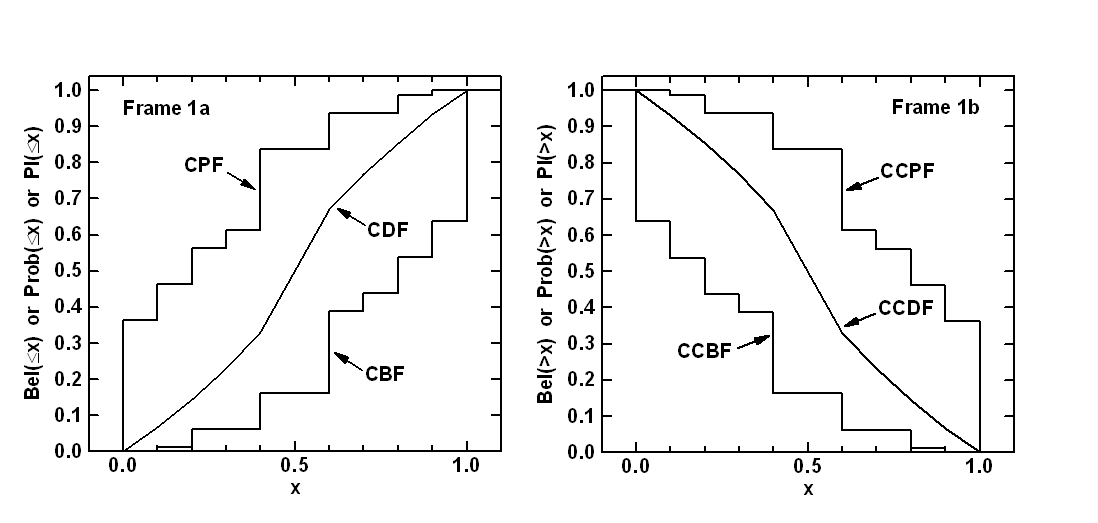
\includegraphics[scale=0.8]{images/belief_plaus} 
  \caption{Example cumulative belief and plausibility distribution functions on left; complementary cumulative belief and plausibility distribution functions on right}
  \label{uq:figure15}
\end{figure}
In evidence theory, it is not possible to specify one probability value.
Instead, there is a range of values that is consistent with the
evidence. The range of values is defined by belief and
plausibility. Note that no statement or claim is made about one value
within an interval being more or less likely than any other value.

In Dempster-Shafer evidence theory, the uncertain input variables are
modeled as sets of intervals. The user assigns a basic probability
assignment (BPA) to each interval, indicating how likely it is that
the uncertain input falls within the interval. The BPAs for a
particular uncertain input variable must sum to one. The intervals
may be overlapping, contiguous, or have gaps. In Dakota, an interval
uncertain variable is specified as \texttt{interval\_uncertain}. When
one defines an interval type variable in Dakota, it is also necessary
to specify the number of intervals defined for each variable with
\texttt{iuv\_num\_intervals} as well the basic probability assignments
per interval, \texttt{iuv\_interval\_probs}, and the associated bounds
per each interval, \texttt{iuv\_interval\_bounds}. 
Figure~\ref{uq:figure16} shows the input specification for interval
uncertain variables. 
The example has two epistemic uncertain interval variables. 
The first uncertain
variable has three intervals and the second has two. The basic
probability assignments for the first variable are 0.5, 0.1, and 0.4,
while the BPAs for the second variable are 0.7 and 0.3. Note that it
is possible (and often the case) to define an interval uncertain
variable with only ONE interval. This means that you only know that
the possible value of that variable falls within the interval, and the
BPA for that interval would be 1.0. In the case we have shown, the
interval bounds on the first interval for the first variable are 0.6
and 0.9, and the bounds for the second interval for the first variable
are 0.1 to 0.5, etc.

\begin{figure}[htbp!]
  \centering
  \begin{bigbox}
    \begin{small}
      \verbatimtabinput[8]{textbook_uq_glob_evidence.in}
    \end{small}
  \end{bigbox}
\caption{Dakota input file for UQ example using Evidence Theory --
see \texttt{Dakota/examples/users/textbook\_uq\_glob\_evidence.in} }
\label{uq:figure16}
\end{figure}

Once the intervals, the BPAs, and the interval bounds are defined, 
the user can run an epistemic analysis by specifying the method as 
either \texttt{global\_evidence} or 
\texttt{local\_evidence} in the Dakota input file. 
Both of these methods perform Dempster-Shafer calculations:  
the difference is that the local method uses a local optimization 
algorithm to calculate the interval bounds and the global 
method uses either sampling or a global optimization approach to 
calculate an interval bound. These differences are discussed in 
more detail below. 
The intervals and their associated BPAs are then propagated through
the simulation to obtain cumulative distribution functions on belief
and plausibility. As mentioned above, belief is the lower bound on a
probability estimate that is consistent with the evidence, and
plausibility is the upper bound on a probability estimate that is
consistent with the evidence. 

Figure~\ref{uq:figure17} shows
results for the first response function obtained when running the
example in Figure~\ref{uq:figure16}. In this example, there are 6
output intervals (as a result of the 2 interval input variables with 3
and 2 intervals, respectively). 
The output intervals are ordered to obtain cumulative
bound functions for both belief and plausibility. The
cumulative distribution function is presented for both belief (CBF) and
plausibility (CPF). The CBF value is the cumulative belief
corresponding to a certain output value. For example, the belief that
the output value is less than or equal to 0.2 for response 1 is 0.27, 
and the plausibility that the output is less than
or equal to 0.2 is 1 for response 1. The belief that the 
output value is less than 0.6217 is 0.75, while the plausbility that 
the output is less than  0.0806 is 0.75. 
The CBF and CPF may be plotted on a graph and
interpreted as bounding the cumulative distribution
function (CDF), which is the probability that the output is less than or equal
to a certain value. The interval bounds on probability values show
the value of epistemic uncertainty analysis: the intervals are usually
much larger than expected, giving one a truer picture of the total
output uncertainty caused by lack of knowledge or information about
the epistemic input quantities.

\begin{figure}[htbp!]
\centering
\begin{bigbox}
\begin{small}
\begin{verbatim}
Belief and Plausibility for each response function:
Cumulative Belief/Plausibility Functions (CBF/CPF) for response_fn_1:
     Response Level  Belief Prob Level   Plaus Prob Level
     --------------  -----------------   ----------------
   1.0000000000e-03   0.0000000000e+00   0.0000000000e+00
   3.0000000000e-02   0.0000000000e+00   2.7000000000e-01
   2.0000000000e-01   2.7000000000e-01   1.0000000000e+00
   8.0000000000e-01   9.3000000000e-01   1.0000000000e+00
  Probability Level  Belief Resp Level   Plaus Resp Level
  -----------------  -----------------   ----------------
   2.5000000000e-01   2.6187288772e-01   6.2609206069e-02
   5.0000000000e-01   2.9829775860e-01   6.3736734971e-02
   7.5000000000e-01   6.2173551556e-01   8.0596931719e-02
\end{verbatim}
\end{small}
\end{bigbox}
\caption{Results of an Epistemic Uncertainty Quantification using Evidence Theory.}
\label{uq:figure17}
\end{figure}

As in other nondeterministic methods, with \texttt{local\_evidence}
or \texttt{global\_evidence},
one can specify probability levels and response levels. 
If response levels are specified, the belief and plausibility 
function values corresponding to those response levels are calculated 
(see Belief Prob Level and Plaus Prob Level in the tables shown in 
Figure~\ref{uq:figure17}). Similarly, if probability levels are 
specified, these are first interpreted to be belief values, and the 
corresponding response levels are calculated (see Belief Resp Level); 
then they are interpreted to be plausibility values and the 
corresponding response levels are calculated (see Plaus Resp Level in 
the table in Figure~\ref{uq:figure17}). We have recently added the 
capability to support generalized reliability mappings in 
the evidence methods. If the user specifies a generalized 
reliability level, it will be first converted to a probability, 
then interpreted as a belief and plausibility and the corresponding 
response levels will be calculated. Likewise, if response levels 
are specified, the corresponding belief and plausibility values 
will be mapped to bounds on the generalized reliability levels. 

To elaborate on the differences between \texttt{global\_evidence} and
\texttt{local\_evidence}: both of these methods take the
Dempster-Shafer structures specified on the inputs and calculate a
resulting Dempster-Shafer structure on the outputs (e.g. a cumulative
belief and plausibility function).  To calculate the belief and
plausibility measures, it is necessary to calculate the minimum and
maximum of the response function in each ``interval cell
combination.''  For example, in a two variable problem, if the first
variable had three intervals and associated BPAs assigned and the
second variable had two intervals and associated BPAs assigned, there
would be 6 interval cells in total.  In each of these six cells, one
needs to identify a minimum and maximum value of the response
function. This is easy to do if the function is monotonic in both
variables, but in general it is not. We offer the capability to use
local optimization methods to calculate these bounds:
\texttt{local\_evidence} allows the user to specify either
\texttt{sqp} which is sequential quadratic programming, or
\texttt{nip} which is a nonlinear interior point method. We also offer
the capability to use global methods to assess these interval cell
bounds. \texttt{global\_evidence} allows the user to specify either
\texttt{lhs}, which performs Latin Hypercube Sampling and takes the
minimum and maximum of the samples within each cell as the bounds (no
optimization is performed) or \texttt{ego}. In the case of
\texttt{ego}, the efficient global optimization method is used to
calculate bounds. The ego method is described in
Section~\ref{opt:methods:gradientfree:global}.  Note that for a
situation with many uncertain variables, each with a fairly
complicated Dempster-Shafer structure described by many intervals,
there will be a huge number of interval calls, and the overall process
of performing Dempster-Shafer analysis will be extremely expensive.
Reference~\cite{Tang10b} provides more details about the
implementation of the optimization methods to perform Dempster-Shafer
calculations, as well as comparisons on test problems.

\section{Bayesian Calibration Methods}\label{uq:bayesian}

There are three implementations of Bayesian calibration methods 
in Dakota, where a ``prior distribution'' on a parameter is 
updated through a Bayesian framework involving experimental data and 
a likelihood function. 
The theory behind Bayesian methods is best described in other sources 
~\cite{Kenn01} and only a brief summary is given here. 
In Bayesian methods, uncertain parameters are characterized by probability 
density functions. These probability densities functions define the 
permissible parameter values - the support, as well as the relative
 plausibility of each permissible parameter value. In the context of 
calibration or any inference step, the probability density function 
that describes knowledge before the incorporation of data is called 
the prior, $f_{\boldsymbol{\Theta}}\left( \boldsymbol{\theta}  \right)$.
 
When data is available, the likelihood function describes how well 
each parameter value is supported by the data. Bayes Theorem~\cite{Jaynes}, 
shown in Equation~\ref{eqn:BayesThm}, is used for inference:  to 
derive the plausible parameter values, based on the prior probability 
density and the data $\boldsymbol{d}$. The result is the posterior parameter density 
of the parameters $f_{\boldsymbol{{\Theta |D}}}\left( \boldsymbol{{\theta |d}} \right)$. It is 
interpreted the same way as the prior, but includes the information 
derived from the data.
 
\begin{equation}
{f_{\boldsymbol{\Theta |D}}}\left( \boldsymbol{\theta |d} \right) = \frac{{{f_{\boldsymbol{\Theta}}}\left( \boldsymbol{\theta}  \right)\mathcal{L}\left( \boldsymbol{\theta;d} \right)}}{{{f_{\boldsymbol{D}}}\left( \boldsymbol{d} \right)}} \label{eq:BayesThm}
\end{equation}


%\begin{equation}
%  \label{eqn:BayesThm}
%  {f_{\Theta |D}}\left( {\theta |d} \right) = \frac{{{f_\Theta }\left( \theta  \right)\mathcal{L}\left( {\theta ;d} \right)}}{{{f_D}\left( d \right)}}
%\end{equation}

The likelihood function is used to describe how well a model's 
predictions are supported by the data. 
The likelihood function can be written generally as:
\begin{equation*}
  \mathcal{L}\left(\boldsymbol{{\theta ;d}} \right) =  \mathcal{F}(q(\boldsymbol{\theta)} -\boldsymbol{d})
\end{equation*}
where $\boldsymbol{\theta}$ are the parameters of model quantity of interest $q$. 
The form of the function $\mathcal{F}$ can greatly influence the results. 
The specific likelihood function used in Dakota is based on 
Gaussian probability density functions. This means that we assume 
the difference between the model quantity (e.g. quantity of interest returned from a computer simulation)
and the experimental observations are Gaussian: 
\begin{equation}\label{eq:model}
d_i = q_i(\boldsymbol{\theta}) + \epsilon_i,
\end{equation}
where $\epsilon_i$ is a random variable that can encompass both
measurement errors on $d_i$ and modeling errors associated with the
simulation quantity of interest $q_i$, for each of $n$ observations.

If we assume that all experiments and observations are independent,
then the probabilistic model defined by Eq.~(\ref{eq:model}) results
in a likelihood function for $\boldsymbol{\theta}$ that is the product of $n$
normal probability density functions:
%as shown in Equation~\ref{eqn:Likelihood}.
\begin{equation}\label{eqn:Likelihood}  
\mathcal{L}(\boldsymbol{{\theta};d}) = \prod_{i=1}^n
\frac{1}{\sigma_d \sqrt{2\pi}} \exp
\left[ - \frac{\left(d_i-q_i(\boldsymbol{{\theta}})\right)^2}{2{\sigma_d}^2} \right],
%\mathcal{L}\left( {{\theta};d} \right) = \prod\limits_{i = 1}^n {\frac{1}{{\sigma \sqrt {2\pi } }}  \exp \left[  - \frac{\left(d_i - \mathcal{M}({\theta})\right)^2}{2\sigma^2} \right]
\end{equation}
where ${\sigma_d}^2$ refers to the measurement error of the data,
assumed constant across all data observations in this case.

We also support the more general case of a full covariance matrix, $\boldsymbol{\Sigma}_d$, that specifies the covariance between each observation $i$ and $j$. 
In this case, the likelihood is commonly written in log form, where the log-likelihood is: %given in Equation~\ref{eqn:LogLikelihood}. 
\begin{equation}\label{eqn:LogLikelihood}  
\log{\mathcal{L}(\boldsymbol{{\theta};d})} \propto % =-0.5 {R}^{T} {\Sigma}^{-1} {R}
-\frac{1}{2} \boldsymbol{r}^T \boldsymbol{\Sigma}_d^{-1} \boldsymbol{r},
\end{equation}
where $\boldsymbol{r}$ is the vector of residuals between the data
points and the model quantity of interest, $q(\boldsymbol{\theta})-\boldsymbol{d}$.

There are now four options to specify the measurement error for
Bayesian calibration methods, with \texttt{variance\_type} being equal
to \texttt{none} for no measurement error specified (in this case, the
variance is one), \texttt{scalar} where a constant value
${\sigma_d}^2$ is given for all observations, \texttt{diagonal} where
a value is specified for the diagonal elements of the covariance
matrix $\Sigma_d$ meaning that each observation has its own
measurement error but there are no cross terms, and \texttt{matrix}
where the full covariance matrix $\Sigma_d$ is specified.  Note that
the \texttt{diagonal} and \texttt{matrix} terms are only available for
field response data.  For scalar responses, variance types
can be specified to be \texttt{none} or \texttt{scalar}.  %Finally,
%all the sigma values should be given as variances (${\sigma_d}^2$).

Markov Chain Monte Carlo (MCMC) is the standard method used to compute
posterior parameter densities, given the observational data and the
priors. There are many references that describe the basic
algorithm~\cite{Gilks}, and in addition, the algorithms are an active
research area.  Note that
MCMC algorithms may require hundreds of thousands of steps to
converge, depending on dimensionality, response nonlinearity, and the
desired set of posterior statistics.  Since each iteration involves an
evaluation of the model to obtain $q(\boldsymbol{\theta})$, surrogate models of
expensive simulations are often employed to make the MCMC process
tractable.
 
As mentioned above, we have three implementations for Bayesian
calibration: QUESO, DREAM, and GPMSA.  They are specified with the
\texttt{bayes\_calibration} keyword in combination with the
\texttt{queso}, \texttt{dream}, or \texttt{gpmsa} selections,
respectively.  The QUESO method uses components from the QUESO library
(Quantification of Uncertainty for Estimation, Simulation, and
Optimization) developed at The University of Texas at Austin.  It
implements the DRAM algorithm, among others.  DRAM indicates the use
of Delayed Rejection and Adaptive Metropolis~\cite{Haario}, where
these two algorithm options can be activated in any combination.
%
DREAM uses an implementation of DiffeRential Evolution Adaptive Metropolis
developed by John Burkardt.  The DREAM approach runs multiple
different chains simultaneously for global exploration, and
automatically tunes the proposal covariance during the process by a
self-adaptive randomized subspace sampling~\cite{Vrugt}.  
%
The GPMSA capability is based on the GPMSA Matlab toolbox developed at
Los Alamos National Laboratory. At this point, the QUESO
implementation is the most well-developed within Dakota and is the one
that we recommend.

In the QUESO method, the user can run the MCMC sampling with 
the simulation model directly. However, 
if the model is expensive, we recommend that the user employs 
a surrogate model (an emulator) because the Monte Carlo Markov Chain 
will be much faster: the MCMC can generate thousands of samples 
on the emulator in very little time. One can specify a Gaussian process,
a polynomial chaos expansion, or a stochastic collocation expansion
as the emulator for the \texttt{queso} method. The specification 
details for these are listed in the Reference Manual. 
One can also specify various settings for the MCMC sampling: 
the sampling can use a standard Metropolis-Hastings algorithm (\texttt{metropolis\_hastings}), adaptive Metropolis (\texttt{adaptive\_metropolis}) for adapting the proposal covariance during the sampling, delayed rejection (\texttt{delayed\_rejection}) for backtracking from sample rejections, the full DRAM (\texttt{dram}) which involves both delayed rejection and adaptive Metropolis, or a multi-level algorithm (\texttt{multilevel}).

There are also controls to specify the proposal covariance which governs how the samples 
are generated in the chain.  
The proposal covariance specifies the covariance structure of a multivariate normal distribution. 
The user can specify \texttt{proposal\_covariance}, followed by \texttt{derivatives}, \texttt{prior}, 
\texttt{values}, or \texttt{filename}.  The derivative specification involves 
forming the Hessian of the misfit function (the negative
log likelihood).  When derivative information is available inexpensively (e.g. from an emulator), 
the derivative-based proposal covariance forms a more
accurate proposal distribution, resulting in lower rejection rates and
faster chain mixing.  Note that the derivative-based proposal covariance 
should be updated periodically based on a \texttt{proposal\_updates} specification.
%may also be updated by adding high-likelihood evaluations of the actual simulation to the emulator build points in an adaptive fashion, thus refining the Hessian.  
The \texttt{prior} setting means that Dakota will form the proposal from the variance of the prior distributions of the 
parameters being calibrated.  When specifying the proposal covariance with values or from a file, the user 
can choose to specify only the diagonals of the covariance matrix or to specify the full covariance matrix.
An additional control for QUESO is to perform a logit transformation (\texttt{logit\_transform}) which 
performs an internal variable transformation from bounded domains to unbounded domains. %in order to reduce sample rejection due to an out-of-bounds condition.
This option can be helpful when regions of high posterior density exist
in the corners of a multi-dimensional bounded domain.  In these cases,
it may be difficult to generate feasible samples from the proposal density,
such that transformation to unbounded domains may greatly reduce sample
rejection rates.
The specification details for keywords governing the proposal covariance are listed in the Reference Manual. 
For more detail about derivative-based formulations involving the misfit Hessian, refer to the Theory Manual. 
    
For the DREAM method, one can define the number of chains used with the
\texttt{chains} specification.  The total number of generations per chain in DREAM is
the number of samples divided by the number of chains.
%The minimum number of chains is three.
The number of chains randomly selected to be used in the crossover
each time a crossover occurs is \texttt{crossover\_chain\_pairs}.
There is an extra adaptation during burn-in, in which DREAM estimates a
distribution of crossover probabilities that favors large jumps over
smaller ones in each of the chains.
Normalization is required to ensure that all of the input dimensions contribute
equally.  In this process, a discrete number of candidate points for
each crossover value is generated, which can be specified with \texttt{num\_cr}.
The \texttt{gr\_threshold} control is the convergence tolerance for the Gelman-Rubin
statistic, which governs the convergence of the multiple chain
process.  The integer \texttt{jump\_step} forces a long jump every 
\texttt{jump\_step} generations.
For more details about these parameters, refer to \cite{Vrugt}. 

For the GPMSA capability, a key part of the algorithm involves the 
construction of an emulator from simulation runs 
collected at various settings of input parameters. The emulator is a 
statistical model of the system response, and it is used to incorporate 
the observational data to improve system predictions and constrain or 
calibrate the unknown parameters. The GPMSA code draws heavily 
on the theory developed in the seminal Bayesian calibration paper 
by Kennedy and O'Hagan~\cite{Kenn01}. The particular approach developed 
by the Los Alamos group is provided in~\cite{Hig08}. GPMSA uses 
Gaussian process models in the emulation, but the emulator is 
actually a set of basis functions (e.g. from a singular value 
decomposition) which have GPs as the coefficients. 
At this point, the GPMSA implementation in Dakota is an early 
prototype. The user will have to edit the GPMSA class in the Dakota 
source to tailor it to their problem and recompile before running GPMSA.
%One major difference between the GPMSA toolbox and the current
%implementation in Dakota is that the current Dakota implementation
%does not have an explicit ``discrepancy'' function $\delta$ which
%models the difference between the simulation and the observational
%data results in addition to the error term $\epsilon$, but GPMSA has a
%sophisticated model for the discrepancy term.

%At this point, the GPMSA library is a standalone C++ library which has 
%its own methods to create Gaussian process models, perform MCMC updating, 
%etc. The GPMSA C++ library is an alpha-version and undergoing development, 
%so a user is cautioned to obtain the latest version (e.g. Version-of-the-Day)
%to have the latest updates. We expect that future Dakota-GPMSA integration 
%will involve more interoperability and sharing of optimization 
%algorithms and surrogate models between Dakota and GPMSA, for example. 

\subsection{Bayesian Calibration Example}\label{uq:bayesian:ex}

We briefly describe the process of running QUESO from Dakota.
The user will create a Dakota input file such as the one shown 
in~\ref{uq:figure18}. 
Note that the method is \texttt{bayes\_calibration queso}, 
specifying the QUESO algorithm with the DRAM (delayed
rejection adaptive metropolis) solver. The number of 
samples indicates the number of samples that the MCMC algorithm 
will generate in its acceptance chain\footnote{If delayed rejection is active, the number of simulation evaluations will typically be higher due to backtracking.}, in this case 1000 (this usually will need to be larger). 
For this example, we are using the \texttt{cantilever3} analytic 
example, so we do not need to specify an emulator, but the lines 
commented out give an idea of the options if the user wanted to 
specify an emulator.  The proposal covariance 
used has diagonal element values of 1.e6 and 0.1.  
The calibration terms in the responses section refers to the 
number of outputs that will be used in the calibration process:  
in this case, it is just two. The calibration data file 
has the observational data:  in this case, it is a freeform file 
(e.g. no header or annotation) with ten experiments. For each 
experiment, there are two experiment values, one for stress and one for displacement, followed 
by two variance values for the error associated with that experiment for each quantity of interest. 

\begin{figure}[htbp!]
\centering
\begin{bigbox}
\begin{small}
\begin{verbatim}
method,
       bayes_calibration queso
#       emulator
#       gp
#        emulator_samples = 50
#        points_file = 'ros.txt' freeform
#       pce 
#        sparse_grid_level = 3 
        samples = 1000  seed = 348                                    
        dram 
        proposal_covariance
         diagonal values 1.0e6 1.0e-1
        logit_transform
         output verbose
 
variables,
       uniform_uncertain = 2
         lower_bounds = 1.0e6 0.1
         upper_bounds = 1.0e8 10.0
         initial_point = 2.85e7 2.5
       continuous_state = 4
          initial_state 3 40000 500 1000
          descriptors 't' 'R' 'X' 'Y'

interface,
         system
           analysis_driver = 'cantilever3'

responses,
        calibration_terms = 2
        calibration_data_file = 'dakota_cantilever_queso.withsigma.dat'
          freeform
          num_experiments = 10
          variance_type = 'scalar'
        descriptors = 'stress' 'displacement'
        no_gradients
        no_hessians
\end{verbatim}
\end{small}
\end{bigbox}
\caption{Dakota input file for UQ example using Bayesian Calibration}
\label{uq:figure18}
\end{figure}

When the input file shown in~\ref{uq:figure18} is run, Dakota will run
the MCMC algorithm and generate a posterior sample of $\boldsymbol{\theta}$ in
accordance with Bayes Theorem~\ref{eqn:BayesThm} and the likelihood
function~\ref{eqn:Likelihood}. Dakota's final output summary will
currently report an evaluation count summary and the best sample point
that was visited during the MCMC process, as measured by maximum
posterior probability (an estimate of the MAP point).

A variety of auxilliary output also exists.  The MCMC sample output is
put into a directory called \texttt{outputData} in the directory from
which Dakota is run.  The file \texttt{display\_sub0.txt} contains
information regarding the MCMC process.  The Matlab files contained in
the \texttt{outputData} directory contain the chain files.  The files
to load in Matlab are \texttt{raw\_chain.m} or
\texttt{filtered\_chain.m}, containing the full chain or the filtered
chain values of the parameters\footnote{The full chain will be output
  in cases of adaptive posterior refinement or proposal updating,
  since these use cases access the entire acceptance chain to identify
  refinement data or restarting points, respectively.}.  There are
corresponding files containing the log likelihood values.  In
addition, if verbose output is specified, the values that Dakota
generates are written to a file in the run directory called
QuesoOutput.txt.  The first columns of this file are the sample
inputs, the next columns are the responses, and the final column is
the log-likelihood.  Note that this file contains ALL values
generated, including the ones rejected, so it is not the actual MCMC
chain which contains only the accepted points.

%We expect to continue development of Bayesian calibration methods, 
%so check for updates to this capability. The QUESO and GPMSA capabilities
%in Dakota currently rely on the QUESO library developed by The University of 
%Texas at Austin. This integrated capability is still in prototype form and 
%available to close collaborators of the Dakota team.  DREAM is distributed 
%with Dakota.
%
%Bayesian methods are currently an active development area within
%Dakota, so we recommend monitoring our updates to these capabilities.
%If you would like additional information on emerging capabilities, 
%contact the Dakota developers at dakota-developers@development.sandia.gov.
  
\section{Uncertainty Quantification Usage Guidelines} \label{usage:uq}

The choice of uncertainty quantification method depends on how the
input uncertainty is characterized, the computational budget, and the
desired output accuracy.  The recommendations for UQ methods are
summarized in Table~\ref{usage:guideuq} and are discussed in the
remainder of the section.

\begin{table}[hbp]
\centering
\caption{Guidelines for UQ method selection.} \label{usage:guideuq}\vspace{2mm}
\begin{tabular}{|c|c|c|}
\hline
\textbf{Method} & \textbf{Desired Problem} & \textbf{Applicable Methods} \\
\textbf{Classification} & \textbf{Characteristics} & \\
\hline
Sampling & nonsmooth, multimodal response functions;       & sampling 
(Monte Carlo or LHS) \\
         & response evaluations are relatively inexpensive & \\
\hline
Local       & smooth, unimodal response functions; & local\_reliability
(MV, AMV/AMV$^2$,\\
reliability & larger sets of random variables;     & AMV+/AMV$^2$+, TANA, 
FORM/SORM) \\
            & estimation of tail probabilities     & \\
\hline
Global      & smooth or limited nonsmooth response; & global\_reliability \\
reliability & multimodal response; low dimensional; & \\
            & estimation of tail probabilities      & \\
\hline
Adaptive    & smooth or limited nonsmooth response; & importance\_sampling, \\
Sampling    & multimodal response; low dimensional; & gpais, adaptive\_sampling, \\
            & estimation of tail probabilities      & pof\_darts \\
\hline
Stochastic & smooth or limited nonsmooth response; & polynomial\_chaos, \\
expansions & multimodal response; low dimensional; & stoch\_collocation\\
           & estimation of moments or moment-based metrics & \\
\hline
Epistemic & uncertainties are poorly characterized &
interval: local\_interval\_est, \\
 & & global\_interval\_est, sampling; \\
 & & BPA: local\_evidence, global\_evidence \\
\hline
Mixed UQ  & some uncertainties are poorly characterized &
nested UQ (IVP, SOP, DSTE) with epistemic \\
 & & outer loop and aleatory inner loop, sampling \\
\hline
\end{tabular}
\end{table}


{\bf Sampling Methods} \\
Sampling-based methods are the most robust uncertainty techniques
available, are applicable to almost all simulations, and possess
rigorous error bounds; consequently, they should be used whenever the
function is relatively inexpensive to compute and adequate sampling
can be performed. In the case of terascale computational simulations,
however, the number of function evaluations required by traditional
techniques such as Monte Carlo and Latin hypercube sampling (LHS)
quickly becomes prohibitive, especially if tail statistics are
needed. %Additional sampling options include quasi-Monte Carlo (QMC)
%sampling and importance sampling (IS),
%or Markov Chain Monte Carlo (MCMC) sampling
%and incremental sampling may also be used to incrementally add samples 
%to an existing sample set.

Alternatively, one can apply the traditional sampling techniques to a
surrogate function approximating the expensive computational
simulation (see Section~\ref{adv_models:sbuq}). However, if this
approach is selected, the user should be aware that it is very
difficult to assess the accuracy of the results obtained. Unlike
the case of surrogate-based local minimization (see
Section~\ref{adv_meth:sbm:sblm}), there is no simple pointwise calculation to
verify the accuracy of the approximate results. This is due to the
functional nature of uncertainty quantification, i.e. the accuracy of
the surrogate over the entire parameter space needs to be considered,
not just around a candidate optimum as in the case of surrogate-based
local. This issue especially manifests itself when trying to estimate
low probability events such as the catastrophic failure of a system.

{\bf Reliability Methods} \\
Local reliability methods (e.g., MV, AMV/AMV$^2$, AMV+/AMV$^2$+, TANA,
and FORM/SORM) are more computationally efficient in general than the
sampling methods and are effective when applied to reasonably
well-behaved response functions; i.e., functions that are smooth,
unimodal, and only mildly nonlinear. They can be used to provide
qualitative sensitivity information concerning which uncertain
variables are important (with relatively few function evaluations), or
compute full cumulative or complementary cumulative response functions
(with additional computational effort). Since they rely on gradient
calculations to compute local optima (most probable points of
failure), they scale well for increasing numbers of random variables,
but issues with nonsmooth, discontinuous, and multimodal response
functions are relevant concerns. In addition, even if there is a
single MPP and it is calculated accurately, first-order and
second-order integrations may fail to accurately capture the shape of
the failure domain. In these cases, adaptive importance sampling
around the MPP can be helpful. Overall, local reliability methods
should be used with some care and their accuracy should be verified
whenever possible.

An effective alternative to local reliability analysis when confronted
with nonsmooth, multimodal, and/or highly nonlinear response functions
is efficient global reliability analysis (EGRA). This technique
employs Gaussian process global surrogate models to accurately resolve
the failure domain and then employs multimodal adaptive importance
sampling to resolve the probabilities. For relatively low dimensional
problems (i.e, on the order of 10 variables), this method displays the
efficiency of local reliability analysis with the accuracy of
exhaustive sampling. While extremely promising, this method is still
relatively new and is the subject of ongoing refinements as we deploy
it to additional applications.

{\bf Adaptive Sampling Methods} \\
There are now a number of methods in Dakota which are tailored to 
estimating tail probabilities.
These methods include both standard importance sampling and 
Gaussian Process Adaptive Importance Sampling, as well as 
adaptive sampling and the POF-darts method. These methods 
are suitable for smooth or limited non-smooth responses, 
and work well in low dimensions. GPAIS and POF-darts utilize 
a Gaussian process surrogate model.  
 
{\bf Stochastic Expansions Methods} \\
The next class of UQ methods available in Dakota is comprised of
stochastic expansion methods (polynomial chaos and stochastic
collocation), which are general purpose techniques provided that the
response functions possess finite second order moments. Further, these
methods capture the underlying functional relationship between a key
response metric and its random variables, rather than just
approximating statistics such as mean and standard deviation. This
class of methods parallels traditional variational methods in
mechanics; in that vein, efforts are underway to compute rigorous
error bounds of the approximations produced by the methods. Another
strength of these methods is their potential use in a multiphysics
environment as a means to propagate the uncertainty through a series
of simulations while retaining as much information as possible at each
stage of the analysis. The current challenge in the development of
these methods, as for other global surrogate-based methods, is
effective scaling for large numbers of random variables. Recent
advances in adaptive collocation and sparsity detection methods
address some of the scaling issues for stochastic expansions.

{\bf Epistemic Uncertainty Quantification Methods} \\
The final class of UQ methods available in Dakota are focused on
epistemic uncertainties, or uncertainties resulting from a lack of
knowledge. In these problems, the assignment of input probability
distributions when data is sparse can be somewhat suspect. One
approach to handling epistemic uncertainties is interval analysis
(\texttt{local\_interval\_est} and \texttt{global\_interval\_est}),
where a set of intervals on inputs, one interval for each input
variable, is mapped to a set of intervals on outputs.  To perform this
process efficiently, optimization methods can be used.  Another
related technique is Dempster-Shafer theory of evidence (Dakota
methods \texttt{local\_evidence} and \texttt{global\_evidence}), where
multiple intervals per input variable (which can be overlapping,
contiguous, or disjoint) are propagated, again potentially using
optimization methods.  The choice between local or global optimization
methods for interval computation is governed by the same issues
described in Section~\ref{opt:usage}.

{\bf Mixed Aleatoric and Epistemic Methods} \\
For problems with a mixture of epistemic and aleatoric uncertainties,
it is desirable to segregate the two uncertainty types within a nested
analysis, allowing stronger probabilistic inferences for the portion
of the problem where they are appropriate. In this nested approach, an
outer epistemic level selects realizations of epistemic parameters
(augmented variables) and/or realizations of random variable
distribution parameters (inserted variables). These realizations
define the objective probabilistic analysis to be performed on the
inner aleatoric level. In the case where the outer loop involves
propagation of subjective probability, the nested approach is known as
second-order probability and the study generates a family of CDF/CCDF
respresentations known as a ``horse tail'' plot.  In the case where
the outer loop is an interval propagation approach
(\texttt{local\_interval\_est} or \texttt{global\_interval\_est}), the
nested approach is known as interval-valued probability (see also
Section~\ref{models:nested}) . In the case where the outer loop is an
evidence-based approach (\texttt{local\_evidence} or
\texttt{global\_evidence}), the approach generates epistemic belief
and plausibility bounds on aleatory statistics.


\begin{comment}
\section{Future Nondeterministic Methods}\label{uq:future}

Uncertainty analysis methods under investigation for future inclusion
into the Dakota framework include extensions to the stochastic
expansion methods and sampling capabilities currently supported.
In particular, smart adaptive methods that can mitigate the curse
of dimensionality are a research emphasis.
%
%Advanced ``smart sampling'' techniques such as bootstrap sampling (BS)
%and Markov chain Monte Carlo simulation (McMC) are being considered.
%We also have an active research focus on adaptive sparse grid methods,
%to more efficiently construct stochastic expansions. 
%
%Efforts have been initiated to allow for non-traditional
%representations of uncertainty. We have implemented Dempster-Shafer
%theory of evidence, and other non-traditional approaches may follow. 
%
We are also currently emphasizing the development of Bayesian methods,
specifically focusing on surrogate-modeling, discrepancy, 
post-processing, and multi-model extensions to the Bayesian
calibration capabilities.
%
%, where a ``prior
%distribution'' on a parameter is updated through a Bayesian framework
%involving experimental data and a likelihood function.
%
%Finally, the tractability and efficacy of the more intrusive
%variant of stochastic finite element/polynomial chaos expansion
%methods, previously mentioned, is being assessed for possible
%implementation in Dakota.
\end{comment}

\chapter{Optimization Capabilities}
\label{opt}

Optimization algorithms work to minimize (or maximize) an objective
function, typically calculated by the user simulation code, subject to
constraints on design variables and responses. Available approaches in
Dakota include well-tested, proven gradient-based, derivative-free
local, and global methods for use in science and engineering design
applications. Dakota also offers more advanced algorithms, e.g., to
manage multi-objective optimization or perform surrogate-based
minimization.  This chapter summarizes optimization problem
formulation, standard algorithms available in Dakota (mostly through
included third-party libraries, see~\ref{opt:libraries}), some
advanced capabilities, and offers usage guidelines.

\section{Optimization Formulations}
\label{opt:formulations}

This section provides a basic introduction to the mathematical
formulation of optimization, problems. The primary goal of this
section is to introduce terms relating to these topics, and is not
intended to be a description of theory or numerical algorithms. For
further details,
consult~\cite{Aro89},~\cite{Gil81},~\cite{Haf92},~\cite{Noc99}, and
~\cite{Van84}.

A general optimization problem is formulated as follows:

\begin{eqnarray}
  \hbox{minimize:} & & f(\mathbf{x})\nonumber\\
  & & \mathbf{x} \in \Re^{n}\nonumber\\
  \hbox{subject to:} & &
  \mathbf{g}_{L} \leq \mathbf{g(x)} \leq \mathbf{g}_U\nonumber\\
  & & \mathbf{h(x)}=\mathbf{h}_{t}\label{opt:formulations:equation01}\\
  & & \mathbf{a}_{L} \leq \mathbf{A}_i\mathbf{x} \leq
  \mathbf{a}_U\nonumber\\
  & & \mathbf{A}_{e}\mathbf{x}=\mathbf{a}_{t}\nonumber\\
  & & \mathbf{x}_{L} \leq \mathbf{x} \leq \mathbf{x}_U\nonumber
\end{eqnarray}

where vector and matrix terms are marked in bold typeface. In this
formulation, $\mathbf{x}=[x_{1},x_{2},\ldots,x_{n}]$ is an
n-dimensional vector of real-valued \emph{design variables} or
\emph{design parameters}. The n-dimensional vectors, $\mathbf{x}_{L}$
and $\mathbf{x}_U$, are the lower and upper bounds, respectively, on
the design parameters. These bounds define the allowable values for
the elements of $\mathbf{x}$, and the set of all allowable values is
termed the \emph{design space} or the \emph{parameter space}. A
\emph{design point} or a \emph{sample point} is a particular set of 
values within the parameter space.

The optimization goal is to minimize the \emph{objective function},
$f(\mathbf{x})$, while satisfying the constraints. Constraints can be
categorized as either linear or nonlinear and as either inequality or
equality. The \emph{nonlinear inequality constraints},
$\mathbf{g(x)}$, are ``2-sided,'' in that they have both lower and
upper bounds, $\mathbf{g}_L$ and $\mathbf{g}_U$, respectively. The
\emph{nonlinear equality constraints}, $\mathbf{h(x)}$, have target
values specified by $\mathbf{h}_{t}$. The linear inequality
constraints create a linear system $\mathbf{A}_i\mathbf{x}$, where
$\mathbf{A}_i$ is the coefficient matrix for the linear system. These
constraints are also 2-sided as they have lower and upper bounds,
$\mathbf{a}_L$ and $\mathbf{a}_U$, respectively. The linear equality
constraints create a linear system $\mathbf{A}_e\mathbf{x}$, where
$\mathbf{A}_e$ is the coefficient matrix for the linear system and
$\mathbf{a}_{t}$ are the target values. The constraints partition the
parameter space into feasible and infeasible regions. A design point
is said to be \emph{feasible} if and only if it satisfies all of the
constraints. Correspondingly, a design point is said to be
\emph{infeasible} if it violates one or more of the constraints.

Many different methods exist to solve the optimization problem given
by Equation~\ref{opt:formulations:equation01}, all of which iterate on
$\mathbf{x}$ in some manner. That is, an initial value for each
parameter in $\mathbf{x}$ is chosen, the \emph{response quantities},
$f(\mathbf{x})$, $\mathbf{g(x)}$, $\mathbf{h(x)}$, are computed, often
by running a simulation, and some algorithm is applied to generate a
new $\mathbf{x}$ that will either reduce the objective function,
reduce the amount of infeasibility, or both. To facilitate a general
presentation of these methods, three criteria will be used in the
following discussion to differentiate them: optimization problem type,
search goal, and search method.

The {\bf optimization problem type} can be characterized both by
the types of constraints present in the problem and by the linearity
or nonlinearity of the objective and constraint functions. For
constraint categorization, a hierarchy of complexity exists for
optimization algorithms, ranging from simple bound constraints,
through linear constraints, to full nonlinear constraints. By the
nature of this increasing complexity, optimization problem
categorizations are inclusive of all constraint types up to a
particular level of complexity. That is, an \emph{unconstrained
  problem} has no constraints, a \emph{bound-constrained problem} has
only lower and upper bounds on the design parameters, a
\emph{linearly-constrained problem} has both linear and bound
constraints, and a \emph{nonlinearly-constrained problem} may contain
the full range of nonlinear, linear, and bound constraints. If all of
the linear and nonlinear constraints are equality constraints, then
this is referred to as an \emph{equality-constrained problem}, and if
all of the linear and nonlinear constraints are inequality
constraints, then this is referred to as an
\emph{inequality-constrained problem}. Further categorizations can be
made based on the linearity of the objective and constraint functions.
A problem where the objective function and all constraints are linear
is called a \emph{linear programming (LP) problem}. These types of
problems commonly arise in scheduling, logistics, and resource
allocation applications. Likewise, a problem where at least some of
the objective and constraint functions are nonlinear is called a
\emph{nonlinear programming (NLP) problem}. These NLP problems
predominate in engineering applications and are the primary focus of
Dakota.

The {\bf search goal} refers to the ultimate objective of the
optimization algorithm, i.e., either global or local optimization. In
\emph{global optimization}, the goal is to find the design point that
gives the lowest feasible objective function value over the entire
parameter space. In contrast, in \emph{local optimization}, the goal
is to find a design point that is lowest relative to a ``nearby''
region of the parameter space. In almost all cases, global
optimization will be more computationally expensive than local
optimization. Thus, the user must choose an optimization algorithm
with an appropriate search scope that best fits the problem goals and
the computational budget.

The {\bf search method} refers to the approach taken in the
optimization algorithm to locate a new design point that has a lower
objective function or is more feasible than the current design point.
The search method can be classified as either \emph{gradient-based} or
\emph{nongradient-based}. In a gradient-based algorithm, gradients of
the response functions are computed to find the direction of
improvement. Gradient-based optimization is the search method that
underlies many efficient local optimization methods. However, a
drawback to this approach is that gradients can be computationally
expensive, inaccurate, or even nonexistent. In such situations,
nongradient-based search methods may be useful. There are numerous
approaches to nongradient-based optimization. Some of the more well
known of these include pattern search methods (nongradient-based local
techniques) and genetic algorithms (nongradient-based global
techniques). 

Because of the computational cost of running simulation
models, surrogate-based optimization (SBO) methods are often used to
reduce the number of actual simulation runs. In SBO, a surrogate or
approximate model is constructed based on a limited number of
simulation runs. The optimization is then performed on the surrogate
model. Dakota has an extensive framework for managing a variety of
local, multipoint, global, and hierarchical surrogates for use in
optimization. Finally, sometimes there are multiple objectives that 
one may want to optimize simultaneously instead of a single scalar 
objective.  In this case, one may employ multi-objective methods 
that are described in Section~\ref{opt:additional:multiobjective}.

This overview of optimization approaches underscores that no single
optimization method or algorithm works best for all types of
optimization problems. Section~\ref{opt:usage} offers guidelines for
choosing a Dakota optimization algorithm best matched to your specific
optimization problem.

\subsection{Constraint Considerations}
\label{opt:formulations:constraints}

Dakota's input commands permit the user to specify two-sided nonlinear
inequality constraints of the form $g_{L_{i}} \leq g_{i}(\mathbf{x})
\leq g_{U_{i}}$, as well as nonlinear equality constraints of the form
$h_{j}(\mathbf{x}) = h_{t_{j}}$. Some optimizers (e.g.,
\texttt{npsol\_}, \texttt{optpp\_}, \texttt{soga}, and \texttt{moga}
methods) can handle these constraint forms directly, whereas other
optimizers (e.g., \texttt{asynch\_pattern\_search}, \texttt{dot\_},
and \texttt{conmin\_}, \texttt{mesh\_adaptive\_search}) require Dakota
to perform an internal conversion of all constraints to one-sided
inequality constraints of the form $g_{i}(\mathbf{x}) \leq 0$. In the
latter case, the two-sided inequality constraints are treated as
$g_{i}(\mathbf{x}) - g_{U_{i}} \leq 0$ and $g_{L_{i}} -
g_{i}(\mathbf{x}) \leq 0$ and the equality constraints are treated as
$h_{j}(\mathbf{x}) - h_{t_{j}} \leq 0$ and $h_{t_{j}} -
h_{j}(\mathbf{x}) \leq 0$. The situation is similar for linear
constraints: \texttt{asynch\_pattern\_search}, \texttt{npsol\_},
\texttt{optpp\_}, \texttt{soga}, and \texttt{moga} methods support
them directly, whereas \texttt{dot\_} and \texttt{conmin\_} methods do
not. For linear inequalities of the form $a_{L_{i}} \leq
\mathbf{a}_{i}^{T}\mathbf{x} \leq a_{U_{i}}$ and linear equalities of
the form $\mathbf{a}_{i}^{T}\mathbf{x} = a_{t_{j}}$, the nonlinear
constraint arrays in \texttt{dot\_} and \texttt{conmin\_} methods are
further augmented to include $\mathbf{a}_{i}^{T}\mathbf{x} - a_{U_{i}}
\leq 0$ and $a_{L_{i}} - \mathbf{a}_{i}^{T}\mathbf{x} \leq 0$ in the
inequality case and $\mathbf{a}_{i}^{T}\mathbf{x} - a_{t_{j}} \leq 0$
and $a_{t_{j}} - \mathbf{a}_{i}^{T}\mathbf{x} \leq 0$ in the equality
case. Awareness of these constraint augmentation procedures can be
important for understanding the diagnostic data returned from the
\texttt{dot\_} and \texttt{conmin\_} methods. Other optimizers fall
somewhere in between.  \texttt{nlpql\_} methods support nonlinear
equality constraints $h_{j}(\mathbf{x}) = 0$ and nonlinear one-sided
inequalities $g_{i}(\mathbf{x}) \geq 0$, but does not natively support
linear constraints. Constraint mappings are used with NLPQL for both
linear and nonlinear cases. Most \texttt{coliny\_} methods now support
two-sided nonlinear inequality constraints and nonlinear constraints
with targets, but do not natively support linear constraints.

When gradient and Hessian information is used in the optimization,
derivative components are most commonly computed with respect to the
active continuous variables, which in this case are the
\emph{continuous design variables}. This differs from parameter study
methods (for which all continuous variables are active) and from
nondeterministic analysis methods (for which the uncertain variables
are active). Refer to Section~\ref{responses:active} for additional
information on derivative components and active continuous variables.

\section{Optimizing with Dakota: Choosing a Method}
\label{opt:methods}

This section summarizes the optimization methods available in
Dakota. We group them according to search method and search goal and
establish their relevance to types of problems. For a summary of this
discussion, see Section~\ref{opt:usage}.

\subsection{Gradient-Based Local Methods}
\label{opt:methods:gradient}

Gradient-based optimizers are best suited for efficient navigation to
a local minimum in the vicinity of the initial point.  They are not
intended to find global optima in nonconvex design spaces.  For global
optimization methods, see~\ref{opt:methods:gradientfree:global}.
Gradient-based optimization methods are highly efficient, with the
best convergence rates of all of the local optimization methods, and
are the methods of choice when the problem is smooth, unimodal, and
well-behaved. However, these methods can be among the least robust
when a problem exhibits nonsmooth, discontinuous, or multimodal
behavior.  The derivative-free methods described
in~\ref{opt:methods:gradientfree:local} are more appropriate for
problems with these characteristics.

Gradient accuracy is a critical factor for gradient-based optimizers,
as inaccurate derivatives will often lead to failures in the search or
pre-mature termination of the method.  Analytic gradients and Hessians
are ideal but often unavailable.  If analytic gradient and Hessian
information can be provided by an application code, a full Newton
method will achieve quadratic convergence rates near the solution. If
only gradient information is available and the Hessian information is
approximated from an accumulation of gradient data, the superlinear
convergence rates can be obtained.  It is most often the case for
engineering applications, however, that a finite difference method
will be used by the optimization algorithm to estimate gradient
values. Dakota allows the user to select the step size for these
calculations, as well as choose between forward-difference and
central-difference algorithms. The finite difference step size should
be selected as small as possible, to allow for local accuracy and
convergence, but not so small that the steps are ``in the noise.''
This requires an assessment of the local smoothness of the response
functions using, for example, a parameter study method. Central
differencing will generally produce more reliable gradients than
forward differencing but at roughly twice the expense.

Gradient-based methods for nonlinear optimization problems can be
described as iterative processes in which a sequence of subproblems,
usually which involve an approximation to the full nonlinear problem,
are solved until the solution converges to a local optimum of the full
problem.  The optimization methods available in Dakota fall into
several categories, each of which is characterized by the nature of
the subproblems solved at each iteration.

\subsubsection{Method Descriptions}
\label{opt:methods:gradient:descriptions}

{\bf Conjugate Gradient} methods require first derivative information
and can only be applied to \emph{unconstrained} problems.  The
subproblems entail minimizing a quadratic function over a space
defined by the gradient and directions that are mutually conjugate
with respect to the Hessian, though the Hessian is never computed.
There are several variants of how those directions are defined.  Those
available in Dakota are the Fletcher-Reeves conjugate gradient method
(\texttt{conmin\_frcg} and \texttt{dot\_frcg}~\cite{Van95}) and the
Polak-Ribiere conjugate gradient method (\texttt{optpp\_cg}).
\emph{We here provide a caution regarding \texttt{dot\_frcg}.  In DOT
  Version 4.20, we have noticed inconsistent behavior of this
  algorithm across different versions of Linux.  Our best assessment
  is that it is due to different treatments of uninitialized
  variables.  As we do not know the intention of the code authors and
  maintaining DOT source code is outside of the Dakota project scope,
  we have not made nor are we recommending any code changes to address
  this.  However, all users who use \texttt{dot\_frcg} in DOT Version
  4.20 should be aware that results may not be reliable.}

{\bf Sequential Quadratic Programming (SQP)} methods are appropriate
for nonlinear optimization problems with nonlinear constraints.  Each
subproblem involves minimizing a quadratic approximation the
Lagrangian subject to linearized constraints.  Only gradient
information is required; Hessians are approximated by low-rank updates
defined by the step taken at each iterations. \emph{It is important to note
that while the solution found by an SQP method will respect the
constraints, the intermediate iterates may not.}  SQP methods available
in Dakota are \texttt{dot\_sqp}, \texttt{nlpql\_sqp}, and
\texttt{npsol\_sqp}~\cite{Gil86}. The particular implementation in
\texttt{nlpql\_sqp}~\cite{Sch04} uses a variant with distributed and
non-monotone line search.  Thus, this variant is designed to be more
robust in the presence of inaccurate or noisy gradients common in many
engineering applications.  Also available is a method related to SQP:
sequential linear programming (\texttt{dot\_slp}).

{\bf Newton Methods} can be applied to nonlinear optimization problems
with nonlinear constraints.  The subproblems associated with these
methods entail finding the solution to a linear system of equations
derived by setting the derivative of a second-order Taylor series
expansion to zero.  Unlike SQP methods, Newton methods maintain
feasibility over the course of the optimization iterations.  The
variants of this approach correspond to the amount of derivative
information provided by the user.  The full Newton method
(\texttt{optpp\_newton}) expects both gradients and Hessians to be
provided.  Quasi-Newton methods (\texttt{optpp\_q\_newton},
\texttt{dot\_bfgs}) expect only gradients.  The Hessian is
approximated by the Broyden-Fletcher-Goldfarb-Shanno (BFGS) low-rank
updates.  Finally, the finite difference Newton method
(\texttt{optpp\_fd\_newton}) expects only gradients and approximates
the Hessian with second-order finite differences.

{\bf Method of Feasible Directions (MFD)} methods are appropriate for
nonlinear optimization problems with nonlinear constraints.  These
methods ensure that all iterates remain feasible.  Dakota includes
\texttt{conmin\_mfd}~\cite{Van78} and \texttt{dot\_mmfd} \emph{One
  observed drawback to \texttt{conmin\_mfd} is that it does a poor job
  handling equality constraints}. \texttt{dot\_mmfd} does not
suffer from this problem, nor do other methods for constrained
problems.

\subsubsection{Example}
\label{opt:methods:gradient:example}

We refer the reader to Section~\ref{tutorial:examples:optimization}
for this example.

\subsection{Derivative-Free Local Methods}
\label{opt:methods:gradientfree:local}

Derivative-free methods can be more robust and more inherently
parallel than gradient-based approaches. They can be applied in
situations were gradient calculations are too expensive or
unreliable. In addition, some derivative-free methods can be used for
global optimization which gradient-based techniques
(see~\ref{opt:methods:gradient}), by themselves,
cannot. For these reasons, derivative-free methods are often go-to
methods when the problem may be nonsmooth, multimodal, or poorly
behaved.  It is important to be aware, however, that they exhibit much
slower convergence rates for finding an optimum, and as a result, tend
to be much more computationally demanding than gradient-based
methods. They often require from several hundred to a thousand or more
function evaluations for local methods, depending on the number of
variables, and may require from thousands to tens-of-thousands of
function evaluations for global methods. Given the computational cost,
it is often prudent to use derivative-free methods to identify regions
of interest and then use gradient-based methods to home in on the
solution.  In addition to slow convergence, nonlinear constraint
support in derivative-free methods is an open area of research and,
while supported by many methods in Dakota, is not as refined as
constraint support in gradient-based methods.

\subsubsection{Method Descriptions}
\label{opt:methods:gradientfree:local:descriptions}

{\bf Pattern Search} methods can be applied to nonlinear optimization
problems with nonlinear.  They generally walk through the domain
according to a defined stencil of search directions.  These methods
are best suited for efficient navigation to a local minimum in the
vicinity of the initial point; however, they sometimes exhibit limited
global identification abilities if the stencil is such that it allows
them to step over local minima.  There are two main pattern search
methods available in Dakota, and they vary according to richness of
available stencil and the way constraints supported.  Asynchronous
Parallel Pattern Search (APPS)~\cite{GrKo06}
(\texttt{asynch\_pattern\_search}) uses the coordinate basis as its
stencil, and it handles nonlinear constraints explicitly through
modification of the coordinate stencil to allow directions that
parallel constraints~\cite{GrKo07}.  A second variant of pattern
search, \texttt{coliny\_pattern\_search}, has the option of using
either a coordinate or a simplex basis as well as allowing more
options for the stencil to evolve over the course of the optimization.
It handles nonlinear constriants through the use of penalty functions.
The
\texttt{mesh\_adaptive\_search}~\cite{AuLeTr09a},~\cite{Nomad},~\cite{Le2011a}
is similar in spirit to and falls in the same class of methods as the
pattern search methods.  The primary difference is that its underlying
search structure is that of a mesh.  The
\texttt{mesh\_adaptive\_search} also provides a unique optimization
capability in Dakota in that it can explicitly treat categorical
variables, i.e., non-relaxable discrete variables as described in
Section~\ref{variables:design:ddv}.

{\bf Simplex} methods for nonlinear optimization problem are similar
to pattern search methods, but their search directions are defined by
triangles that are reflected, expanded, and contracted across the
variable space.  The two simplex-based methods available in Dakota are
the Parallel Direct Search method~\cite{Den94b} (\texttt{optpp\_pds})
and the Constrained Optimization BY Linear Approximations (COBYLA)
(\texttt{coliny\_cobyla}).  The former handles only bound constraints,
while the latter handles nonlinear constraints.  \emph{One drawback of
  both simplex-based methods is that their current implementations do
  not allow them to take advantage of parallel computing resources via
  Dakota's infrastructure.}

A {\bf Greedy Search Heuristic} for nonlinear optimization problems is
captured in the Solis-Wets (\texttt{coliny\_solis\_wets}) method.
This method takes a sampling-based approach in order to identify
search directions.  \emph{Note that one observed drawback to
  \texttt{coliny\_solis\_wets} is that it does a poor job solving
  problems with nonlinear constraints.  This algorithm is also not
  implemented in such a way as to take advantage of parallel computing
  resources via Dakota's infrastructure.}

\subsubsection{Example}
\label{opt:methods:gradientfree:local:example}

The Dakota input file shown in
Figure~\ref{opt:methods:gradientfree:local:example:ps} applies a
pattern search method to minimize the Rosenbrock function. We note
that this example is used as a means of demonstrating the contrast
between input files for gradient-based and derivative-free
optimization.  Since derivatives can be computed analytically and
efficiently, the preferred approach to solving this problem is a
gradient-based method.

The Dakota input file shown in
Figure~\ref{opt:methods:gradientfree:local:example:ps} is similar to
the input file for the gradient-based optimization, except it has a
different set of keywords in the method block of the input file, and
the gradient specification in the responses block has been changed to
\texttt{no\_gradients}. The pattern search optimization algorithm
used, \texttt{coliny\_pattern\_search} is part of the SCOLIB
library~\cite{Har06}. See the Dakota Reference Manual~\cite{RefMan}
for more information on the \emph{methods} block commands that can be
used with SCOLIB algorithms.

\begin{figure}[ht!]
  \centering
  \begin{bigbox}
    \begin{small}
      \verbatimtabinput[8]{rosen_opt_patternsearch.in}
    \end{small}
  \end{bigbox}
  \caption{Rosenbrock pattern search optimization example: the Dakota input file --
see \texttt{Dakota/examples/users/rosen\_opt\_patternsearch.in} }
  \label{opt:methods:gradientfree:local:example:ps}
\end{figure}

For this run, the optimizer was given an initial design point of
$(x_1,x_2) = (0.0,0.0)$ and was limited to 2000 function
evaluations. In this case, the pattern search algorithm stopped short
of the optimum at $(x_1,x_2) = (1.0,1,0)$, although it was making
progress in that direction when it was terminated. (It would have
reached the minimum point eventually.)

The iteration history is provided in Figures~
\ref{opt:methods:gradientfree:local:example:ps_graphics}(a) and (b),
which show the locations of the function evaluations used in the
pattern search algorithm.
Figure~\ref{opt:methods:gradientfree:local:example:ps_graphics}(c)
provides a close-up view of the pattern search function evaluations
used at the start of the algorithm. The coordinate pattern is clearly
visible at the start of the iteration history, and the decreasing size
of the coordinate pattern is evident at the design points move toward
$(x_1,x_2) = (1.0,1.0)$.

\begin{figure}[ht!]
  \centering
  \begin{tabular}{cc}
  \multicolumn{2}{c}
	      {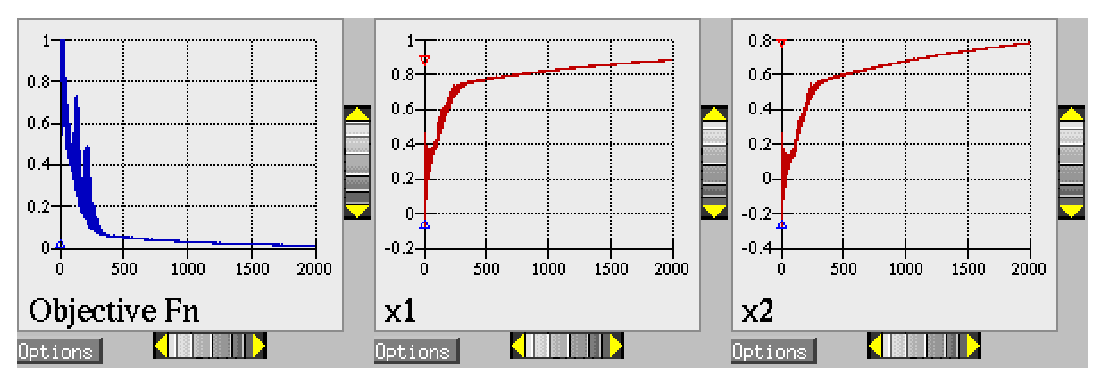
\includegraphics[width=\textwidth]{images/dak_graphics_ps_opt}}\\
  \multicolumn{2}{c}{(a)}\\
  \qquad\\
  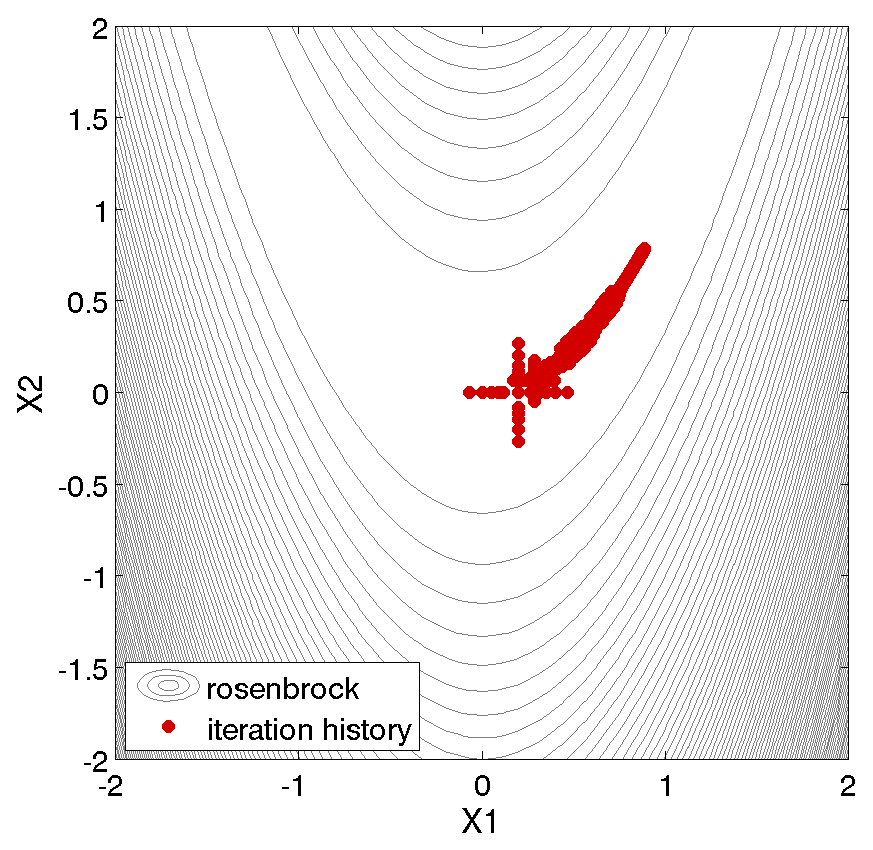
\includegraphics[height=2.5in]{images/rosen_ps_opt_pts} &
  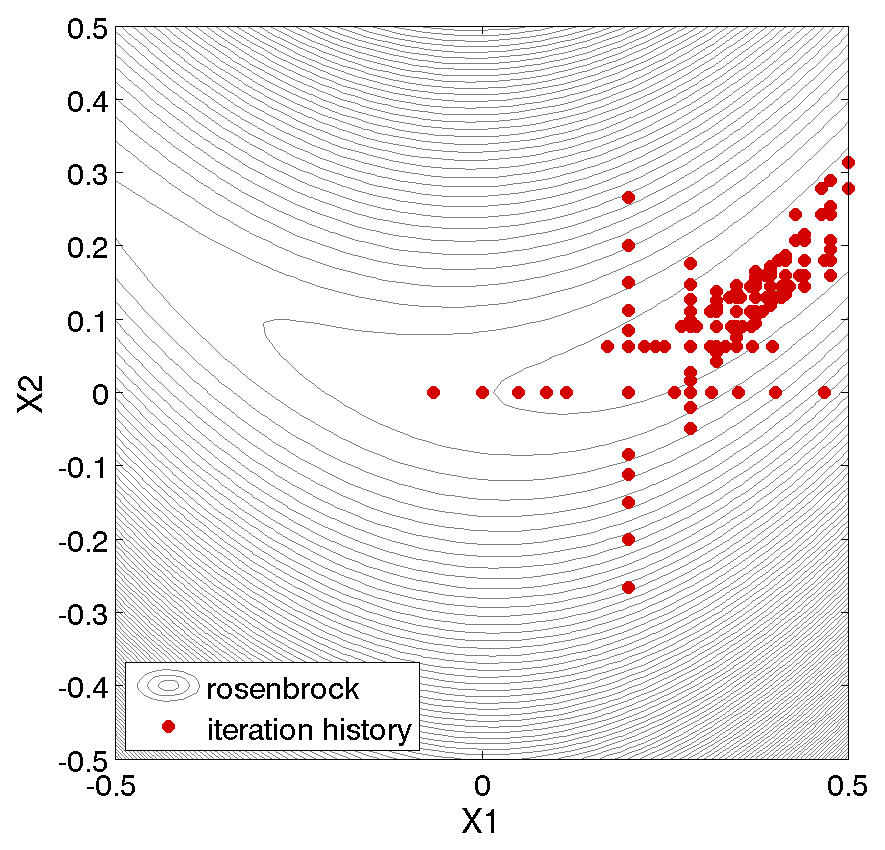
\includegraphics[height=2.5in]{images/rosen_ps_opt_pts2} \\
  (b) & (c)
  \end{tabular}
  \caption{Rosenbrock pattern search optimization example: (a) screen
    capture of the Dakota graphics, (b) sequence of design points
    (dots) evaluated and (c) close-up view illustrating the shape of
    the coordinate pattern used. }
  \label{opt:methods:gradientfree:local:example:ps_graphics}
\end{figure}

While pattern search algorithms are useful in many optimization
problems, this example shows some of the drawbacks to this algorithm.
While a pattern search method may make good initial progress towards
an optimum, it is often slow to converge. On a smooth, differentiable
function such as Rosenbrock's function, a nongradient-based method
will not be as efficient as a gradient-based method. However, there
are many engineering design applications where gradient information is
inaccurate or unavailable, which renders gradient-based optimizers
ineffective. Thus, pattern search algorithms are often good choices in
complex engineering applications when the quality of gradient data is
suspect.

\subsection{Derivative-Free Global Methods}
\label{opt:methods:gradientfree:global}

The discussion of derivative-free global methods is identical to that
in~\ref{opt:methods:gradientfree:local}, so we forego repeating it
here.  There are two types of global optimization methods in Dakota.

\subsubsection{Method Descriptions}
\label{opt:methods:gradientfree:global:descriptions}

{\bf Evolutionary Algorithms (EA)} are based on Darwin's theory of
survival of the fittest. The EA algorithm starts with a randomly
selected population of design points in the parameter space, where the
values of the design parameters form a ``genetic string,'' analogous
to DNA in a biological system, that uniquely represents each design
point in the population. The EA then follows a sequence of
generations, where the best design points in the population (i.e.,
those having low objective function values) are considered to be the
most ``fit'' and are allowed to survive and reproduce. The EA
simulates the evolutionary process by employing the mathematical
analogs of processes such as natural selection, breeding, and
mutation. Ultimately, the EA identifies a design point (or a family of
design points) that minimizes the objective function of the
optimization problem. An extensive discussion of EAs is beyond the
scope of this text, but may be found in a variety of sources (cf.,
~\cite{Haf92} pp. 149-158;~\cite{Gol89}). EAs available in Dakota
include \texttt{coliny\_ea}, \texttt{soga}, and \texttt{moga}.  The
latter is specifically designed for multi-objective problems,
discussed further in~\ref{opt:additional}.  All variants can optimize
over discrete variables, including discrete string variables, in
addition to continuous variables.  We note that an experimental branch
and bound capability is being matured to provide a gradient-based
approach to solving mixed variable global optimization problems.  One
key distinction is that it does not handle categorical variables
(e.g., string variables).  The branch and bound method is discussed
further in Section~\ref{adv_meth:minlp}.

{\bf DIvision of RECTangles (DIRECT)}~\cite{Gab01} balances local
search in promising regions of the design space with global search in
unexplored regions.  It adaptively subdivides the space of feasible
design points to guarantee that iterates are generated in the
neighborhood of a global minimum in finitely many iterations.  Dakota
includes two implementations (\texttt{ncsu\_direct} and
\texttt{coliny\_direct}.  In practice, DIRECT has proven an effective
heuristic for many applications.  For some problems, the
\texttt{ncsu\_direct} implementation has outperformed the
\texttt{coliny\_direct} implementation.  \texttt{ncsu\_direct} can
accommodate only bound constraints, while \texttt{coliny\_direct}
handles nonlinear constraints using a penalty formulation of the
problem.

{\bf Efficient Global Optimization (EGO)} is a global optimization
technique that employs response surface surrogates~\cite{Jon98,Hua06}.
In each EGO iteration, a Gaussian process (GP) approximation for the
objective function is constructed based on sample points of the true
simulation.  The GP allows one to specify the prediction at a new
input location as well as the uncertainty associated with that
prediction.  The key idea in EGO is to maximize an Expected
Improvement Function (EIF), defined as the expectation that any point
in the search space will provide a better solution than the current
best solution, based on the expected values and variances predicted by
the GP model.  It is important to understand how the use of this EIF
leads to optimal solutions.  The EIF indicates how much the objective
function value at a new potential location is expected to be less than
the predicted value at the current best solution.  Because the GP
model provides a Gaussian distribution at each predicted point,
expectations can be calculated.  Points with good expected values and
even a small variance will have a significant expectation of producing
a better solution (exploitation), but so will points that have
relatively poor expected values and greater variance (exploration).
The EIF incorporates both the idea of choosing points which minimize
the objective and choosing points about which there is large
prediction uncertainty (e.g., there are few or no samples in that area
of the space, and thus the probability may be high that a sample value
is potentially lower than other values).  Because the uncertainty is
higher in regions of the design space with few observations, this
provides a balance between exploiting areas of the design space that
predict good solutions, and exploring areas where more information is
needed.

There are two major differences between our implementation and that of
~\cite{Jon98}: we do not use a branch and bound method to find points
which maximize the EIF.  Rather, we use the DIRECT algorithm.  Second,
we allow for multiobjective optimization and nonlinear least squares
including general nonlinear constraints.  Constraints are handled
through an augmented Lagrangian merit function approach (see
Surrogate-Based Minimization chapter in Dakota Theory
Manual~\cite{TheoMan}).

\subsubsection{Examples}
\label{opt:methods:gradientfree:global:example}

{\bf Evolutionary algorithm:} In contrast to pattern search
algorithms, which are local optimization methods, evolutionary
algorithms (EA) are global optimization methods. As was described
above for the pattern search algorithm, the Rosenbrock function is not
an ideal test problem for showcasing the capabilities of evolutionary
algorithms. Rather, EAs are best suited to optimization problems that
have multiple local optima, and where gradients are either too
expensive to compute or are not readily available.

\begin{figure}[ht!]
  \centering
  \begin{bigbox}
    \begin{small}
      \verbatimtabinput[8]{rosen_opt_ea.in}
    \end{small}
  \end{bigbox}
  \caption{Rosenbrock evolutionary algorithm optimization example: the
  Dakota input file --
see \texttt{Dakota/examples/users/rosen\_opt\_ea.in} }
  \label{opt:methods:gradientfree:global:example:rosenbrock_ea}
\end{figure}

Figure~\ref{opt:methods:gradientfree:global:example:rosenbrock_ea}
shows a Dakota input file that uses an EA to minimize the Rosenbrock
function. For this example the EA has a population size of 50. At the
start of the first generation, a random number generator is used to
select 50 design points that will comprise the initial
population. \emph{[A specific seed value is used in this example to
  generate repeatable results, although, in general, one should use
  the default setting which allows the EA to choose a random seed.]} A
two-point crossover technique is used to exchange genetic string
values between the members of the population during the EA breeding
process. The result of the breeding process is a population comprised
of the 10 best ``parent'' design points (elitist strategy) plus 40 new
``child'' design points. The EA optimization process will be
terminated after either 100 iterations (generations of the EA) or
2,000 function evaluations. The EA software available in Dakota
provides the user with much flexibility in choosing the settings used
in the optimization process. See~\cite{RefMan} and~\cite{Har06} for
details on these settings.

The EA optimization results printed at the end of this file show that
the best design point found was $(x_1,x_2) = (0.98,0.95)$. The file
\texttt{ea\_tabular.dat.sav} provides a listing of the design
parameter values and objective function values for all 2,000 design
points evaluated during the running of the EA. Figure~
\ref{opt:methods:gradientfree:global:example:rosenbrock_ea_graphics}(a)
shows the population of 50 randomly selected design points that
comprise the first generation of the EA, and
Figure~\ref{opt:methods:gradientfree:global:example:rosenbrock_ea_graphics}(b)
shows the final population of 50 design points, where most of the 50
points are clustered near $(x_1,x_2) = (0.98,0.95)$.

\begin{figure}[hbt!]
  \centering
  \begin{tabular}{cc}
  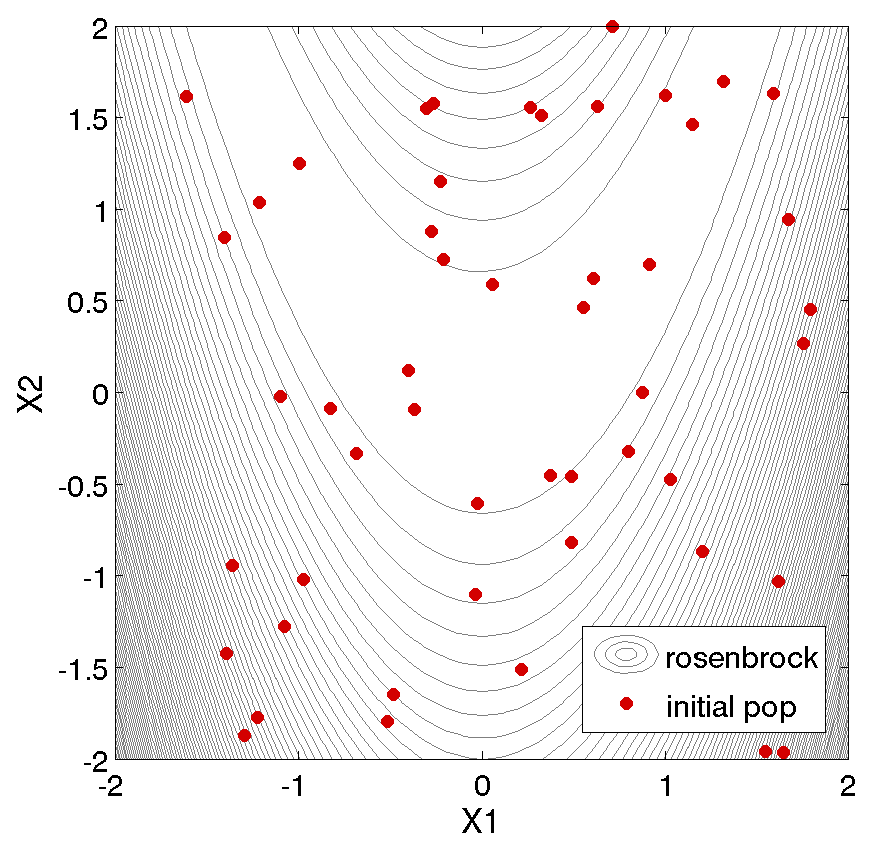
\includegraphics[height=2.5in]{images/rosen_ea_init} &
  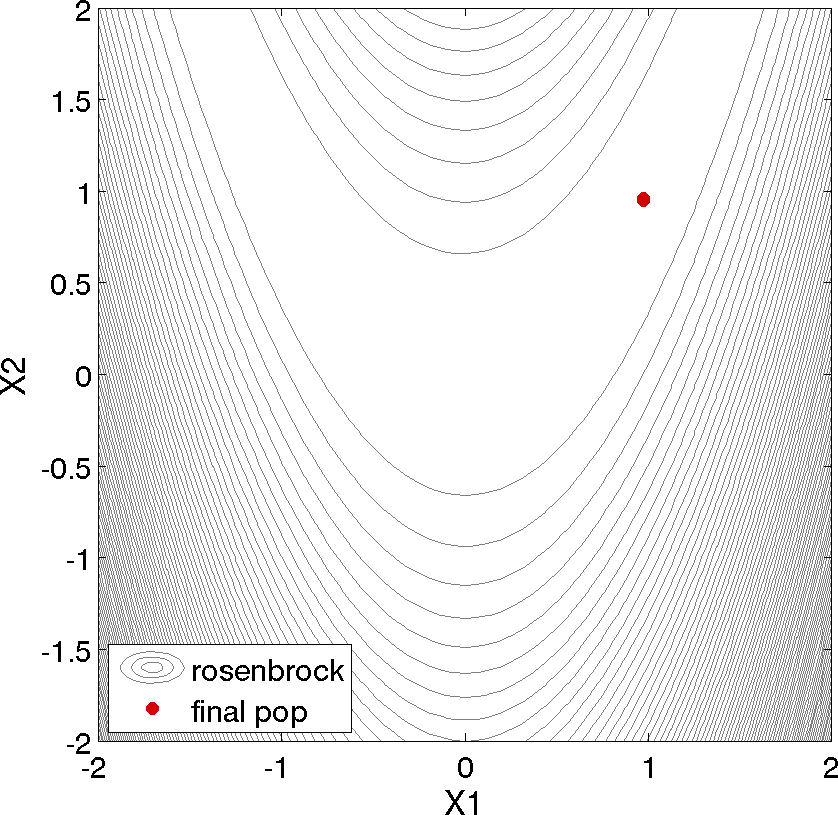
\includegraphics[height=2.5in]{images/rosen_ea_final} \\
  (a) & (b)
  \end{tabular}
  \caption{Rosenbrock evolutionary algorithm optimization example: 50
    design points in the (a) initial and (b) final populations
    selected by the evolutionary algorithm. }
  \label{opt:methods:gradientfree:global:example:rosenbrock_ea_graphics}
\end{figure}

As described above, an EA is not well-suited to an optimization
problem involving a smooth, differentiable objective such as the
Rosenbrock function. Rather, EAs are better suited to optimization
problems where conventional gradient-based optimization fails, such as
situations where there are multiple local optima and/or gradients are
not available. In such cases, the computational expense of an EA is
warranted since other optimization methods are not applicable or
impractical. In many optimization problems, EAs often quickly identify
promising regions of the design space where the global minimum may be
located. However, an EA can be slow to converge to the optimum. For
this reason, it can be an effective approach to combine the global
search capabilities of a EA with the efficient local search of a
gradient-based algorithm in a \emph{hybrid optimization} strategy. In
this approach, the optimization starts by using a few iterations of a
EA to provide the initial search for a good region of the parameter
space (low objective function and/or feasible constraints), and then
it switches to a gradient-based algorithm (using the best design point
found by the EA as its starting point) to perform an efficient local
search for an optimum design point. More information on this hybrid
approach is provided in Section~\ref{adv_meth:hybrid}.

{\bf Efficient Global Optimization:} The method is specified as
\texttt{efficient\_global}.  Currently we do not expose any
specification controls for the underlying Gaussian process model used
or for the optimization of the expected improvement function, which is
currently performed by the NCSU DIRECT algorithm. The only item the
user can specify is a seed which is used in the Latin Hypercube
Sampling to generate the initial set of points which is used to
construct the initial Gaussian process.  An example specification for
the EGO algorithm is shown in Figure~\ref{opt:methods:gradientfree:global:example:egm_rosen}.
\begin{figure}
  \begin{bigbox}
    \begin{small}
      \verbatimtabinput[8]{rosen_opt_ego.in}
    \end{small}
  \end{bigbox}
  \caption{Dakota input file for the efficient global optimization example --
see \texttt{Dakota/examples/users/rosen\_opt\_ego.in} }
  \label{opt:methods:gradientfree:global:example:egm_rosen}
\end{figure}


\section{Additional Optimization Capabilities}
\label{opt:additional}

Dakota provides several capabilities which extend the services
provided by the optimization software packages described in
Sections~\ref{opt:methods:gradient}
through~\ref{opt:methods:gradientfree:global}. Those described in this
section include:
\begin{itemize}
\item {\bf Multiobjective optimization}: There are three capabilities
  for multiobjective optimization in Dakota. The first is MOGA,
  described above in
  Section~\ref{opt:methods:gradientfree:global:descriptions}. The
  second is the Pareto-set strategy, described in
  Section~\ref{adv_meth:pareto}. The third is a weighting factor approach for
  multiobjective reduction, in which a composite objective function is
  constructed from a set of individual objective functions using a
  user-specified set of weighting factors. These latter two approaches
  work with any of the above single objective algorithms. Future
  multiobjective response data transformations for goal programming,
  normal boundary intersection, etc. are planned.
\item {\bf Scaling,} where any optimizer (or least squares solver
  described in Section~\ref{nls:solution}), can accept user-specified
  (and in some cases automatic or logarithmic) scaling of continuous
  design variables, objective functions (or least squares terms), and
  constraints. Some optimization algorithms are sensitive to the
  relative scaling of problem inputs and outputs, and this feature can
  help.
\item {\bf Solvers in shared libraries}: On computer systems that
  permit use of shared libraries (most modern systems), Dakota can
  avail itself of optimization solvers contained in shared libraries.
  This is a first step toward allowing optional parts of Dakota, such
  as proprietary solvers, to be accessed from shared
  libraries.\end{itemize}
The Advanced Methods Chapter~\ref{adv_meth} offers details on the 
following component-based meta-algorithm approaches:
\begin{itemize}
\item \textbf{Sequential Hybrid Minimization}: This meta-algorithm
  allows the user to specify a sequence of minimization methods, with
  the results from one method providing the starting point for the
  next method in the sequence. An example which is useful in many
  engineering design problems involves the use of a nongradient-based
  global optimization method (e.g., genetic algorithm) to identify a
  promising region of the parameter space, which feeds its results
  into a gradient-based method (quasi-Newton, SQP, etc.) to perform an
  efficient local search for the optimum point.

\item \textbf{Multistart Local Minimization}: This meta-algorithm uses
  many local minimization runs (often gradient-based), each of which
  is started from a different initial point in the parameter
  space. This is an attractive approach in situations where multiple
  local optima are known to exist or may potentially exist in the
  parameter space. This approach combines the efficiency of local
  minimization methods with the parameter space coverage of a global
  stratification technique.

\item \textbf{Pareto-Set Minimization}: The Pareto-set minimization
  strategy allows the user to specify different sets of weights for
  either the individual objective functions in a multiobjective
  optimization problem or the individual residual terms in a least
  squares problem. Dakota executes each of these weighting sets as a
  separate minimization problem, serially or in parallel, and then
  outputs the set of optimal designs which define the Pareto
  set. Pareto set information can be useful in making trade-off
  decisions in engineering design problems.
\end{itemize}

\subsection{Multiobjective Optimization}
\label{opt:additional:multiobjective}

Multiobjective optimization means that there are two or more objective
functions that you wish to optimize simultaneously. Often these are
conflicting objectives, such as cost and performance. The answer to a
multi-objective problem is usually not a single point. Rather, it is a
set of points called the Pareto front. Each point on the Pareto front
satisfies the Pareto optimality criterion, which is stated as follows:
a feasible vector $X^{*}$ is Pareto optimal if there exists no other
feasible vector $X$ which would improve some objective without causing
a simultaneous worsening in at least one other objective. Thus, if a
feasible point $X'$ exists that CAN be improved on one or more
objectives simultaneously, it is not Pareto optimal: it is said to be
``dominated'' and the points along the Pareto front are said to be
``non-dominated.''

There are three capabilities for multiobjective optimization in
Dakota. First, there is the MOGA capability described previously in
Section~\ref{opt:methods:gradientfree:global:descriptions}. This is a
specialized algorithm capability. The second capability involves the
use of response data transformations to recast a multiobjective
problem as a single-objective problem. Currently, Dakota supports the
simple weighted sum approach for this transformation, in which a
composite objective function is constructed from a set of individual
objective functions using a user-specified set of weighting
factors. This approach is optimization algorithm independent, in that
it works with any of the optimization methods listed previously in
this chapter.  The third capability is the Pareto-set meta-algorithm
described in Section~\ref{adv_meth:pareto}. This capability also
utilizes the multiobjective response data transformations to allow
optimization algorithm independence; however, it builds upon the basic
approach by computing sets of optima in order to generate a Pareto
trade-off surface.

In the multiobjective transformation approach in which multiple
objectives are combined into one, an appropriate single-objective
optimization technique is used to solve the problem. The advantage of
this approach is that one can use any number of optimization methods
that are especially suited for the particular problem class. One
disadvantage of the weighted sum transformation approach is that a
linear weighted sum objective will only find one solution on the
Pareto front.  Since each optimization of a single weighted objective
will find only one point near or on the Pareto front, many
optimizations need to be performed to get a good parametric
understanding of the influence of the weights.  Thus, this approach
can become computationally expensive.

The selection of a multiobjective optimization problem is made through
the specification of multiple objective functions in the responses
keyword block (i.e., the \texttt{objective\_functions} specification
is greater than \texttt{1}). The weighting factors on these objective
functions can be optionally specified using the \texttt{weights}
keyword (the default is equal weightings). The composite objective
function for this optimization problem, $F$, is formed using these
weights as follows: $F=\sum_{k=1}^{R}w_{k}f_{k}$, where the $f_{k}$
terms are the individual objective function values, the $w_{k}$ terms
are the weights, and $R$ is the number of objective functions. The
weighting factors stipulate the relative importance of the design
concerns represented by the individual objective functions; the higher
the weighting factor, the more dominant a particular objective
function will be in the optimization process. Constraints are not
affected by the weighting factor mapping; therefore, both constrained
and unconstrained multiobjective optimization problems can be
formulated and solved with Dakota, assuming selection of an
appropriate constrained or unconstrained single-objective optimization
algorithm.  Future multiobjective response data transformations for
goal programming, normal boundary intersection, etc. are planned.

\subsubsection{Multiobjective Example 1}
\label{opt:additional:multiobjective:example1}

Figure~\ref{opt:additional:multiobjective:example1:figure01} shows a
Dakota input file for a multiobjective optimization problem based on
the ``textbook'' test problem.  In the standard textbook formulation,
there is one objective function and two constraints. In the
multiobjective textbook formulation, all three of these functions are
treated as objective functions (\texttt{objective\_functions = 3}),
with weights given by the \texttt{weights} keyword. Note that it is
not required that the weights sum to a value of one. The
multiobjective optimization capability also allows any number of
constraints, although none are included in this example.

\begin{figure}
\centering
\begin{bigbox}
\begin{small}
\verbatimtabinput[8]{textbook_opt_multiobj1.in}
\end{small}
\end{bigbox}
\caption{Example Dakota input file for multiobjective optimization --
see \texttt{Dakota/examples/users/textbook\_opt\_multiobj1.in} }
\label{opt:additional:multiobjective:example1:figure01}
\end{figure}

Figure~\ref{opt:additional:multiobjective:example1:figure02} shows an
excerpt of the results for this multiobjective optimization problem,
with output in verbose mode. The data for function evaluation 9 show
that the simulator is returning the values and gradients of the three
objective functions and that this data is being combined by Dakota
into the value and gradient of the composite objective function, as
identified by the header ``\texttt{Multiobjective
  transformation:}''. This combination of value and gradient data from
the individual objective functions employs the user-specified
weightings of \texttt{.7}, \texttt{.2}, and \texttt{.1}. Convergence
to the optimum of the multiobjective problem is indicated in this case
by the gradient of the composite objective function going to zero (no
constraints are active).

\begin{figure}
\centering
\begin{bigbox}
\begin{small}
\begin{verbatim}
   ------------------------------
   Begin Function Evaluation    9
   ------------------------------
   Parameters for function evaluation 9:
                         5.9388064483e-01 x1
                         7.4158741198e-01 x2

   (text_book /tmp/fileFNNH3v /tmp/fileRktLe9)
   Removing /tmp/fileFNNH3v and /tmp/fileRktLe9

   Active response data for function evaluation 9:
   Active set vector = { 3 3 3 } Deriv vars vector = { 1 2 }
                         3.1662048106e-02 obj_fn_1
                        -1.8099485683e-02 obj_fn_2
                         2.5301156719e-01 obj_fn_3
    [ -2.6792982175e-01 -6.9024137415e-02 ] obj_fn_1 gradient
    [  1.1877612897e+00 -5.0000000000e-01 ] obj_fn_2 gradient
    [ -5.0000000000e-01  1.4831748240e+00 ] obj_fn_3 gradient



   -----------------------------------
   Post-processing Function Evaluation
   -----------------------------------
   Multiobjective transformation:
                         4.3844693257e-02 obj_fn
    [  1.3827084219e-06  5.8620632776e-07  ] obj_fn gradient

       7    1 1.0E+00    9  4.38446933E-02 1.5E-06    2 T TT     

    Exit NPSOL - Optimal solution found.

    Final nonlinear objective value =   0.4384469E-01
\end{verbatim}
\end{small}
\end{bigbox}
\caption{Dakota results for the multiobjective optimization example.}
\label{opt:additional:multiobjective:example1:figure02}
\end{figure}

By performing multiple optimizations for different sets of weights, a
family of optimal solutions can be generated which define the
trade-offs that result when managing competing design concerns. This
set of solutions is referred to as the Pareto set.
Section~\ref{adv_meth:pareto} describes an algorithm for
directly generating the Pareto set in order to investigate the
trade-offs in multiobjective optimization problems.

\subsubsection{Multiobjective Example 2}
\label{opt:additional:multiobjective:example2}

This example illustrates the use of multi-objective optimization based
on a genetic algorithm method. This method is called \texttt{moga}. It
is based on the idea that as the population evolves in a GA, solutions
that are non-dominated are chosen to remain in the population.  The
MOGA algorithm has separate fitness assessment and selection operators
called the \texttt{domination\_count} fitness assessor and
\texttt{below\_limit} selector respectively.  This approach of
selection works especially well on multi-objective problems because it
has been specifically designed to avoid problems with aggregating and
scaling objective function values and transforming them into a single
objective. Instead, the fitness assessor works by ranking population
members such that their resulting fitness is a function of the number
of other designs that dominate them. The \texttt{below\_limit}
selector then chooses designs by considering the fitness of each. If
the fitness of a design is above a certain limit, which in this case
corresponds to a design being dominated by more than a specified
number of other designs, then it is discarded. Otherwise it is kept
and selected to go to the next generation. The one catch is that this
selector will require that a minimum number of selections take
place. The \texttt{shrinkage\_percentage} determines the minimum
number of selections that will take place if enough designs are
available. It is interpreted as a percentage of the population size
that must go on to the subsequent generation. To enforce this, the
\texttt{below\_limit} selector makes all the selections it would make
anyway and if that is not enough, it relaxes its limit and makes
selections from the remaining designs. It continues to do this until
it has made enough selections.  The moga method has many other
important features. Complete descriptions can be found in the Dakota
Reference Manual~\cite{RefMan}.
 
We demonstrate the MOGA algorithm on three examples that are taken
from a multiobjective evolutionary algorithm (MOEA) test suite
described by Van Veldhuizen et. al. in~\cite{Coe02}. These three
examples illustrate the different forms that the Pareto set may
take. For each problem, we describe the Dakota input and show a graph
of the Pareto front. These problems are all solved with the
\texttt{moga} method.  The first example is presented below, the other
two examples are presented in the additional examples chapter
~\ref{additional:multiobjective:problem2} and
~\ref{additional:multiobjective:problem3}.

In Van Veldhuizen's notation, the set of all Pareto optimal design
configurations (design variable values only) is denoted $\mathtt{P^*}$
or $\mathtt{P_{true}}$ and is defined as:
\begin{eqnarray*}
  P^*:=\{x\in\Omega\,|\,\neg\exists\,\,
  x^\prime\in\Omega\quad\bar{f}(x^\prime)\preceq\bar{f}(x)\}
\end{eqnarray*}
 
The Pareto front, which is the set of objective function values
associated with the Pareto optimal design configurations, is denoted
$\mathtt{PF^*}$ or $\mathtt{PF_{true}}$ and is defined as:
\begin{eqnarray*}
  PF^*:=\{\bar{u}=\bar{f}=(f_1(x),\ldots,f_k(x))\,|\, x\in P^*\}
\end{eqnarray*}
 
The values calculated for the Pareto set and the Pareto front using
the moga method are close to but not always exactly the true values,
depending on the number of generations the moga is run, the various
settings governing the GA, and the complexity of the Pareto set.
 
The first test problem is a case where $P_{true}$ is connected and
$PF_{true}$ is concave. The problem is to simultaneously optimize
$f_1$ and $f_2$ given three input variables, $x_1$, $x_2$, and $x_3$,
where the inputs are bounded by $-4 \leq x_{i} \leq 4$:
 
Figure~\ref{opt:additional:multiobjective:example2:moga1inp} shows an
input file that demonstrates some of the multi-objective capabilities
available with the moga method.
\begin{figure}[htp!]
  \centering
  \begin{bigbox}
    \begin{small}
      \verbatimtabinput[8]{mogatest1.in}
    \end{small}
  \end{bigbox}
  \caption{Multiple objective genetic algorithm (MOGA) example: the
    Dakota input file --
see \texttt{Dakota/examples/users/mogatest1.in} }
  \label{opt:additional:multiobjective:example2:moga1inp}
\end{figure}
 
In this example, the three best solutions (as specified by
\texttt{final\_solutions} =3) are written to the output. Additionally,
final results from moga are output to a file called
\texttt{finaldata1.dat} in the directory in which you are
running. This \texttt{finaldata1.dat} file is simply a list of inputs
and outputs. Plotting the output columns against each other allows one
to see the Pareto front generated by \texttt{moga}.
Figure~\ref{opt:additional:multiobjective:example2:moga_pareto} shows
an example of the Pareto front for this problem. Note that a Pareto
front easily shows the tradeoffs between Pareto optimal solutions. For
instance, look at the point with f1 and f2 values equal to (0.9,
0.23). One cannot improve (minimize) the value of objective function
f1 without increasing the value of f2: another point on the Pareto
front, (0.63, 0.63) represents a better value of objective f1 but a
worse value of objective f2.
\begin{figure}[ht!]
  \centering
  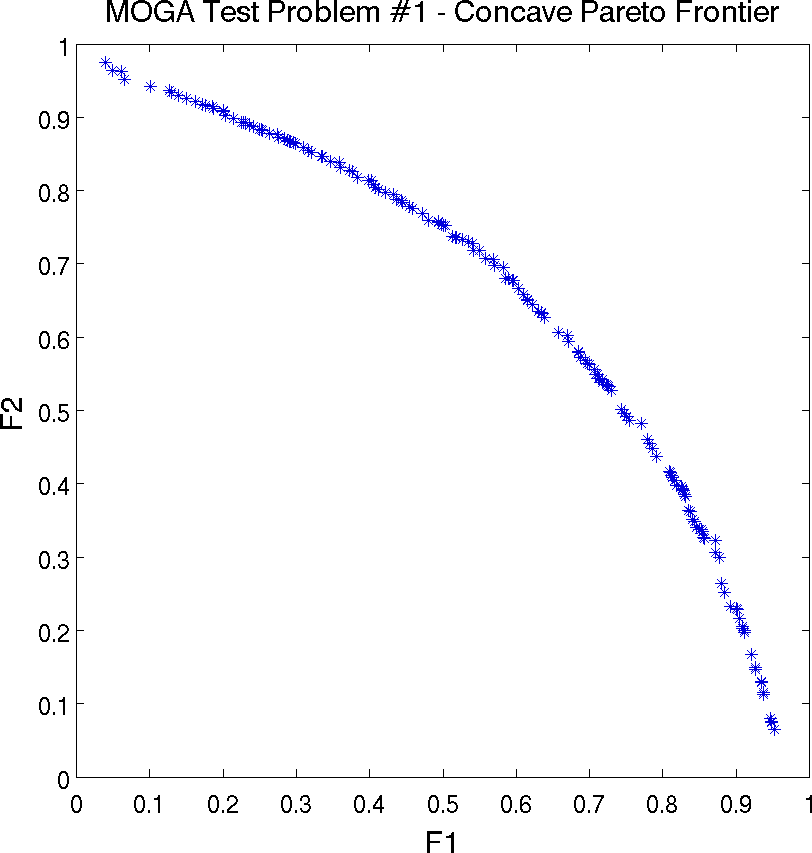
\includegraphics[scale=0.75]{images/dakota_mogatest1_pareto_front}
  \caption{Multiple objective genetic algorithm (MOGA) example: Pareto
  front showing tradeoffs between functions f1 and f2.}
  \label{opt:additional:multiobjective:example2:moga_pareto}
\end{figure}


\subsection{Optimization with User-specified or Automatic Scaling}
\label{opt:additional:scaling}

Some optimization problems involving design variables, objective
functions, or constraints on vastly different scales may be solved
more efficiently if these quantities are adjusted to a common scale
(typically on the order of unity). With any optimizer (or least
squares solver described in Section~\ref{nls:solution}),
user-specified characteristic value scaling may be applied to any of
continuous design variables, functions/residuals, nonlinear inequality
and equality constraints, and linear inequality and equality
constraints. Automatic scaling is available for variables or responses
with one- or two-sided bounds or equalities and may be combined with
user-specified scaling values. Logarithmic ($\log_{10}$) scaling is
available and may also be combined with characteristic values. Log
scaling is not available for linear constraints. Moreover, when
continuous design variables are log scaled, linear constraints are not
permitted in the problem formulation. Discrete variable scaling is not
supported.

Scaling is enabled on a per-method basis for optimizers and least
squares minimizers by including the {\tt scaling} keyword in the
relevant {\tt method} specification in the Dakota input deck. When
scaling is enabled, variables, functions, gradients, Hessians, etc.,
are transformed such that the optimizer iterates in scaled variable
space, whereas evaluations of the computational model as specified in
the interface are performed on the original problem scale. Therefore
using scaling does not require rewriting the interface to the
simulation code. When the {\tt scaling} keyword is omitted, all {\tt
  *\_scale\_types} and {\tt *\_scales} specifications described below
are ignored in the corresponding method, variables, and responses
sections. When the method {\tt output\_level} is set above normal,
scaling initialization and diagnostic information will be printed.

Scaling for a particular variable or response type is enabled through
the {\tt *\_scale\_types} specification (see the Reference Manual
method section and references contained therein for a complete keyword
list). Valid options for this string specification include {\tt
  'none'} (default), {\tt 'value'}, {\tt 'auto'}, or {\tt 'log'}, for
no, characteristic value, automatic, or logarithmic scaling,
respectively (although not all types are valid for scaling all
entities). If a single string is specified with any of these keywords
it will apply to each component of the relevant vector, e.g., {\tt
  cdv\_scale\_types = 'value'} will enable characteristic value
scaling for each continuous design variable.

The user may additionally specify no, one, or a vector of
characteristic scale values through the {\tt *\_scales} specification.
These characteristic values are ignored for scaling type {\tt 'none'},
required for {\tt 'value'}, and optional for {\tt 'auto'} and {\tt
  'log'}. If a single value is specified with any of these keywords it
will apply to each component of the relevant vector, e.g., {\tt
  cdv\_scales = 3.0} will apply a characteristic scaling value of 3.0
to each continuous design variable.

When scaling is enabled, the following procedures determine the
transformations used to scale each component of a variables or
response vector. A warning is issued if scaling would result in
division by a value smaller in magnitude than {\tt 1.0e10*DBL\_MIN}.
User-provided values violating this lower bound are accepted
unaltered, whereas for automatically calculated scaling, the lower
bound is enforced.

\begin{itemize}

\item None ({\tt 'none'}): no scaling performed ({\tt *\_scales}
ignored) on this component.

\item Characteristic value ({\tt 'value'}): the corresponding quantity
  is scaled (divided) by the required characteristic value provided in
  the {\tt *\_scales} specification, and bounds are adjusted as
  necessary. If the value is negative, the sense of inequalities are
  changed accordingly.

\item Automatic ({\tt 'auto'}): First, any characteristic values from
  the optional {\tt *\_scales} specification are applied. Then,
  automatic scaling will be attempted according to the following
  scheme:

  \begin{itemize}
  
  \item two-sided bounds scaled into the interval [0,1];
	
  \item one-sided bounds or targets are scaled by a characteristic
    value to move the bound or target to 1, and the sense of
    inequalities are changed if necessary;

  \item no bounds or targets: no automatic scaling possible for this component
    
  \end{itemize}

  Automatic scaling is not available for objective functions nor least
  squares terms since they lack bound constraints. Further, when
  automatically scaled, linear constraints are scaled by
  characteristic values only, not affinely scaled into [0,1].

\item Logarithmic ({\tt 'log'}): First, any characteristic values from
  the optional {\tt *\_scales} specification are applied. Then,
  $\log_{10}$ scaling is applied. Logarithmic scaling is not available
  for linear constraints. Further, when continuous design variables
  are log scaled, linear constraints are not allowed.

\end{itemize}

Scaling for linear constraints specified through {\tt
  linear\_inequality\_scales} or {\tt linear\_equality\_scales} is
applied {\em after} any (user-specified or automatic) continuous
variable scaling. For example, for scaling mapping unscaled continuous
design variables $x$ to scaled variables $\tilde{x}$:
\[ \tilde{x}^j = \frac{x^j - x^j_O}{x^j_M}, \]
where $x^j_M$ is the final component multiplier and $x^j_O$ the
offset, we have the following matrix system for linear inequality
constraints
\begin{eqnarray*}
& a_L \leq A_i x \leq a_U \\
& a_L \leq A_i \left( \mathrm{diag}(x_M) \tilde{x} + x_O \right) \leq a_U \\
& a_L - A_i x_O \leq A_i \mathrm{diag}(x_M) \tilde{x} \leq a_U - A_i x_O \\
& \tilde{a}_L \leq \tilde{A}_i \tilde{x} \leq \tilde{a}_U,
\end{eqnarray*}
and user-specified or automatically computed scaling multipliers are
applied to this final transformed system, which accounts for any
continuous design variable scaling. When automatic scaling is in use
for linear constraints they are linearly scaled by characteristic
values only, not affinely scaled into the interval $[0,1]$.

\subsubsection{Scaling Example}
\label{opt:additional:scaling:example}

Figure~\ref{opt:additional:scaling:example:figure01} demonstrates the
use of several scaling keywords for the textbook optimization problem.
The continuous design variable {\tt x1} is scaled by a characteristic
value of 4.0, whereas {\tt x2} is scaled automatically into $[0,1]$
based on its bounds. The objective function will be scaled by a factor
of 50.0, then logarithmically, the first nonlinear constraint by a
factor of 15.0, and the second nonlinear constraint is not scaled.

\begin{figure}
\centering
\begin{bigbox}
\begin{small}
\verbatimtabinput[8]{rosen_opt_scaled.in}
\end{small}
\end{bigbox}
\caption{Sample usage of scaling keywords in Dakota input specification --
see \texttt{Dakota/examples/users/rosen\_opt\_scaled.in} }
\label{opt:additional:scaling:example:figure01}
\end{figure}

\subsection{dl\_solver --- Solvers via Shared Libraries}
\label{opt:additional:dlsolver}

On computer systems that permit use of shared libraries (most modern
systems), Dakota can avail itself of optimization solvers contained in
shared libraries.  This is a first step toward allowing optional parts
of Dakota, such as proprietary solvers, to be accessed from shared
libraries. For example, the Dakota source distributions illustrate
making a sample shared-library interface to SNOPT~\cite{GilMS05},
whose use would be specified by
\begin{small}
\begin{verbatim}
    method,
          dl_solver = 'dl_snopt.dll'
\end{verbatim}
\end{small}
The quoted string contains the name of the shared library, optionally
followed by keyword assignments known to the library, such as
\begin{small}
\begin{verbatim}
    method,
          dl_solver = 'dl_snopt.dll outlev = 1'
\end{verbatim}
\end{small}
which would turn on some diagnostic printing in the SNOPT example.

\section{Optimization Usage Guidelines}
\label{opt:usage}

In selecting an optimization method, important considerations include
the type of variables in the problem (continuous, discrete, mixed),
whether a global search is needed or a local search is sufficient, and
the required constraint support (unconstrained, bound constrained, or
generally constrained). Less obvious, but equally important,
considerations include the efficiency of convergence to an optimum
(i.e., convergence rate) and the robustness of the method in the
presence of challenging design space features (e.g., nonsmoothness).

Table~\ref{opt:usage:guideopt} provides a convenient reference for
choosing an optimization method or strategy to match the
characteristics of the user's problem, where blank fields inherit the
value from above. With respect to constraint support, it should be
understood that the methods with more advanced constraint support are
also applicable to the lower constraint support levels; they are
listed only at their highest level of constraint support for brevity.

\begin{table}[hbp]
\centering
\caption{Guidelines for optimization method selection.} 
\label{opt:usage:guideopt}\vspace{2mm}
\begin{tabular}{|c|c|c|}
\hline
\textbf{Method} & \textbf{Desired Problem} & \textbf{Applicable Methods} \\
\textbf{Classification} & \textbf{Characteristics} & \\
\hline
Gradient-Based Local & smooth; continuous variables; no constraints
& optpp\_cg \\
\hline
         & smooth; continuous variables; & dot\_bfgs, dot\_frcg, conmin\_frcg \\
         & bound constraints &  \\
\hline
         & smooth; continuous variables; & npsol\_sqp, nlpql\_sqp, dot\_mmfd, \\
         & bound constraints, & dot\_slp, dot\_sqp,
         conmin\_mfd, \\
         & linear and nonlinear constraints & optpp\_newton,
         optpp\_q\_newton, \\
         &          &optpp\_fd\_newton, \\
         &          & weighted sums (multiobjective), \\
         &          & pareto\_set strategy (multiobjective) \\
\hline
Gradient-Based Global & smooth; continuous variables; & hybrid\_strategy, \\
         &  bound constraints, & multi\_start strategy \\
         &  linear and nonlinear constraints & \\
\hline
Derivative-Free Local & nonsmooth; continuous variables; bound constraints
& optpp\_pds \\
\hline
         & nonsmooth; continuous variables; & asynch\_pattern\_search, \\
         & bound constraints, & coliny\_cobyla, coliny\_pattern\_search, \\
         & linear and nonlinear constraints & coliny\_solis\_wets, \\
         &          & surrogate\_based\_local \\
\hline
         & nonsmooth; continuous variables; &  \\
         & discrete variables; bound constraints, & mesh\_adaptive\_search \\
         & nonlinear constraints &  \\
\hline
Derivative-Free Global & nonsmooth; continuous variables; bound constraints
& ncsu\_direct \\
\hline
         & nonsmooth; continuous variables; & coliny\_direct, efficient\_global, \\
         & bound constraints, & surrogate\_based\_global \\
         & linear and nonlinear constraints & \\
\hline
         & nonsmooth; continuous variables, & coliny\_ea, soga, \\
         & discrete variables; bound constraints, & moga (multiobjective) \\
         & linear and nonlinear constraints & \\
\hline
\end{tabular}
\end{table}

{\bf Gradient-based Methods} \\
Gradient-based optimization methods are highly efficient, with the
best convergence rates of all of the optimization methods. If analytic
gradient and Hessian information can be provided by an application
code, a full Newton method will provide quadratic convergence rates
near the solution. More commonly, only gradient information is
available and a quasi-Newton method is chosen in which the Hessian
information is approximated from an accumulation of gradient data. In
this case, superlinear convergence rates can be obtained. These
characteristics make gradient-based optimization methods the methods
of choice when the problem is smooth, unimodal, and
well-behaved. However, when the problem exhibits nonsmooth,
discontinuous, or multimodal behavior, these methods can also be the
least robust since inaccurate gradients will lead to bad search
directions, failed line searches, and early termination, and the
presence of multiple minima will be missed.

Thus, for gradient-based optimization, a critical factor is the
gradient accuracy. Analytic gradients are ideal, but are often
unavailable. For many engineering applications, a finite difference
method will be used by the optimization algorithm to estimate gradient
values. Dakota allows the user to select the step size for these
calculations, as well as choose between forward-difference and
central-difference algorithms. The finite difference step size should
be selected as small as possible, to allow for local accuracy and
convergence, but not so small that the steps are ``in the noise.''
This requires an assessment of the local smoothness of the response
functions using, for example, a parameter study method. Central
differencing, in general, will produce more reliable gradients than
forward differencing, but at roughly twice the expense.

{\bf Non-gradient-based Methods} \\
Nongradient-based methods exhibit much slower convergence rates for
finding an optimum, and as a result, tend to be much more
computationally demanding than gradient-based methods. Nongradient
local optimization methods, such as pattern search algorithms, often
require from several hundred to a thousand or more function
evaluations, depending on the number of variables, and nongradient
global optimization methods such as genetic algorithms may require
from thousands to tens-of-thousands of function evaluations. Clearly,
for nongradient optimization studies, the computational cost of the
function evaluation must be relatively small in order to obtain an
optimal solution in a reasonable amount of time. In addition,
nonlinear constraint support in nongradient methods is an open area of
research and, while supported by many nongradient methods in Dakota,
is not as refined as constraint support in gradient-based
methods. However, nongradient methods can be more robust and more
inherently parallel than gradient-based approaches. They can be
applied in situations were gradient calculations are too expensive or
unreliable. In addition, some nongradient-based methods can be used
for global optimization which gradient-based techniques, by
themselves, cannot. For these reasons, nongradient-based methods
deserve consideration when the problem may be nonsmooth, multimodal,
or poorly behaved.

{\bf Surrogate-based Methods} \\ Approaches that seek to improve the
effectiveness or efficiency of optimizers and least squares methods
through the use of surrogate models include the surrogate-based local,
surrogate-based global, and efficient global
methods. Section~\ref{adv_meth:sbm} provides further information on
these approaches. The surrogate-based local approach (see
Section~\ref{adv_meth:sbm:sblm}) brings the efficiency of
gradient-based optimization/least squares methods to nonsmooth or
poorly behaved problems by smoothing noisy or discontinuous response
results with a data fit surrogate model (e.g., a quadratic polynomial)
and then minimizing on the smooth surrogate using efficient
gradient-based techniques. The surrogate-based global approach (see
Section~\ref{adv_meth:sbm:sbgm}) similarly employs optimizers/least
squares methods with surrogate models, but rather than localizing
through the use of trust regions, seeks global solutions using global
methods.  And the efficient global approach (see
Section~\ref{opt:methods:gradientfree:global}) uses the specific combination of
Gaussian process surrogate models in combination with the DIRECT
global optimizer. Similar to these surrogate-based approaches, the
hybrid and multistart optimization component-based algorithms seek to bring the
efficiency of gradient-based optimization methods to global
optimization problems. In the former case, a global optimization
method can be used for a few cycles to locate promising regions and
then local gradient-based optimization is used to efficiently converge
on one or more optima. In the latter case, a stratification technique
is used to disperse a series of local gradient-based optimization runs
through parameter space. Without surrogate data smoothing, however,
these strategies are best for smooth multimodal
problems. Section~\ref{adv_meth:hybrid} and
Section~\ref{adv_meth:multistart} provide more information on these
approaches.

\section{Optimization Third Party Libraries}
\label{opt:libraries}

As mentioned in~\ref{opt}, Dakota serves as a delivery vehicle for a
number third-party optimization libraries. The packages are listed
here along with the license status and web page where available.

\begin{itemize}

\item CONMIN (\texttt{conmin\_} methods) License: Public Domain
  (NASA).

\item DOT (\texttt{dot\_} methods) License: commercial; website:
  Vanderplaats Research and Development,
  \url{http://www.vrand.com}. {\em Not included in the open source
    version of Dakota.  Sandia National Laboratories and Los Alamos
    National Laboratory have limited seats for DOT. Other users may
    obtain their own copy of DOT and compile it with the Dakota source
    code.}

\item HOPSPACK (\texttt{asynch\_pattern\_search}) License: LGPL; web
  page: \url{https://software.sandia.gov/trac/hopspack}.

\item JEGA (\texttt{soga}, \texttt{moga}) License: LGPL

\item NCSUOpt (\texttt{ncsu\_direct}) License: MIT

\item NLPQL (\texttt{nlpql\_} methods) License: commercial; website:
  Prof. Klaus Schittkowski,
  \url{http://www.uni-bayreuth.de/departments/math/~kschittkowski/nlpqlp20.htm}). \emph{Not included in the open source version of Dakota.  Users may
    obtain their own copy of NLPQLP and compile it with the Dakota
    source code.}

\item NPSOL (\texttt{npsol\_} methods) License: commercial; website:
  Stanford Business Software
  \url{http://www.sbsi-sol-optimize.com}. {\em Not included in the
    open source version of Dakota.  Sandia National Laboratories,
    Lawrence Livermore National Laboratory, and Los Alamos National
    Laboratory all have site licenses for NPSOL. Other users may
    obtain their own copy of NPSOL and compile it with the Dakota
    source code.}

\item NOMAD (\texttt{mesh\_adaptive\_search}) License: LGPL; website:
  \url{http://www.gerad.ca/NOMAD/Project/Home.html}.

\item OPT++ (\texttt{optpp\_} methods) License: LGPL; website:
  \url{http://csmr.ca.sandia.gov/opt++}.

\item SCOLIB (\texttt{coliny\_} methods) License: BSD; website:
  \url{https://software.sandia.gov/trac/acro/wiki/Packages}

\end{itemize}


\chapter{Nonlinear Least Squares Capabilities}\label{nls}
% TODO: discuss calibration overall, then NLS
\section{Overview}\label{nls:overview}
Any Dakota optimization algorithm can be applied to calibration
problems arising in parameter estimation, system identification, and
test/analysis reconciliation. However, nonlinear least-squares
methods are optimization algorithms that exploit the special structure
of a sum of the squares objective function~\cite{Gil81}.

To exploit the problem structure, more granularity is needed in the
response data than is required for a typical optimization problem.
That is, rather than using the sum-of-squares objective function and
its gradient, least-squares iterators require each term used in the
sum-of-squares formulation along with its gradient. This means that
the $m$ functions in the Dakota response data set consist of the
individual least-squares terms along with any nonlinear inequality and
equality constraints. These individual terms are often called
\emph{residuals} when they denote differences of observed quantities
from values computed by the model whose parameters are being
estimated.

The enhanced granularity needed for nonlinear least-squares algorithms
allows for simplified computation of an approximate Hessian matrix.
In Gauss-Newton-based methods for example, the true Hessian matrix is
approximated by neglecting terms in which residuals multiply Hessians
(matrices of second partial derivatives) of residuals, under the
assumption that the residuals tend towards zero at the solution. As a
result, residual function value and gradient information (first-order
information) is sufficient to define the value, gradient, and
approximate Hessian of the sum-of-squares objective function
(second-order information). See Section~\ref{nls:formulations} for
additional details on this approximation.

In practice, least-squares solvers will tend to be significantly more
efficient than general-purpose optimization algorithms when the
Hessian approximation is a good one, e.g., when the residuals tend
towards zero at the solution. Specifically, they can exhibit the
quadratic convergence rates of full Newton methods, even though only
first-order information is used. Gauss-Newton-based least-squares
solvers may experience difficulty when the residuals at the solution
are significant. Dakota has three solvers customized to take
advantage of the sum of squared residuals structure in this problem
formulation. Least squares solvers may experience difficulty when the
residuals at the solution are significant, although experience has
shown that Dakota's NL2SOL method can handle some problems that are
highly nonlinear and have nonzero residuals at the solution.

\section{Nonlinear Least Squares Fomulations}\label{nls:formulations}

Specialized least squares solution algorithms can exploit the
structure of a sum of the squares objective function for problems of
the form:

\begin{eqnarray}
  \hbox{minimize:} & & f(\mathbf{x}) =
  \sum_{i=1}^{n}[T_i(\mathbf{x})]^2\nonumber\\
  & & \mathbf{x} \in \Re^{n}\nonumber\\
  \hbox{subject to:} & &
  \mathbf{g}_L \leq \mathbf{g(x)} \leq \mathbf{g}_U\nonumber\\
  & & \mathbf{h(x)}=\mathbf{h}_{t}\label{nls:equation02}\\
  & & \mathbf{a}_L \leq \mathbf{A}_i\mathbf{x} \leq
  \mathbf{a}_U\nonumber\\
  & & \mathbf{A}_e\mathbf{x}=\mathbf{a}_{t}\nonumber\\
  & & \mathbf{x}_L \leq \mathbf{x} \leq \mathbf{x}_U\nonumber
\end{eqnarray}

where $f(\mathbf{x})$ is the objective function to be minimized and
$T_i(\mathbf{x})$ is the i$^{\mathrm{th}}$ least squares term. The
bound, linear, and nonlinear constraints are the same as described
previously for (\ref{opt:formulations:equation01}). Specialized least
squares algorithms are generally based on the Gauss-Newton
approximation. When differentiating $f(\mathbf{x})$ twice, terms of
$T_i(\mathbf{x})T''_i(\mathbf{x})$ and $[T'_i(\mathbf{x})]^{2}$
result. By assuming that the former term tends toward zero near the
solution since $T_i(\mathbf{x})$ tends toward zero, then the Hessian
matrix of second derivatives of $f(\mathbf{x})$ can be approximated
using only first derivatives of $T_i(\mathbf{x})$. As a result,
Gauss-Newton algorithms exhibit quadratic convergence rates near the
solution for those cases when the Hessian approximation is accurate,
i.e. the residuals tend towards zero at the solution. Thus, by
exploiting the structure of the problem, the second order convergence
characteristics of a full Newton algorithm can be obtained using only
first order information from the least squares terms.

A common example for $T_i(\mathbf{x})$ might be the difference
between experimental data and model predictions for a response
quantity at a particular location and/or time step, i.e.:

\begin{equation}
  T_i(\mathbf{x}) = R_i(\mathbf{x})-\overline{R_i}
  \label{nls:equation03}
\end{equation}

where $R_i(\mathbf{x})$ is the response quantity predicted by the
model and $\overline{R_i}$ is the corresponding experimental data.
In this case, $\mathbf{x}$ would have the meaning of model parameters
which are not precisely known and are being calibrated to match
available data. This class of problem is known by the terms parameter
estimation, system identification, model calibration, test/analysis
reconciliation, etc.

\section{Nonlinear Least Squares with Dakota}

In order to specify a least-squares problem, the responses section of
the Dakota input should be configured using
\texttt{calibration\_terms} (as opposed to
\texttt{num\_objective\_functions} in the case of optimization). The
calibration terms refer to the residuals (e.g. typically the
differences between the simulation model and the data). Note that
Dakota expects the residuals and not the square of the residuals. Any
linear or nonlinear constraints are handled in an identical way to
that of optimization (see Section~\ref{opt:formulations}; note that
neither Gauss-Newton nor NLSSOL require any constraint augmentation
and NL2SOL supports neither linear nor nonlinear constraints).
Gradients of the least-squares terms and nonlinear constraints are
required and should be specified using either
\texttt{numerical\_gradients}, \texttt{analytic\_gradients}, or
\texttt{mixed\_gradients}. Since explicit second derivatives are not
used by the least-squares methods, the \texttt{no\_hessians}
specification should be used. Dakota's scaling options, described in
Section~\ref{opt:additional:scaling} can be used on least-squares
problems, using the \texttt{calibration\_term\_scales} keyword to
scale least-squares residuals, if desired.

\section{Solution Techniques}\label{nls:solution}

Nonlinear least-squares problems can be solved using the Gauss-Newton
algorithm, which leverages the full Newton method from OPT++, the
NLSSOL algorithm, which is closely related to NPSOL, or the NL2SOL
algorithm, which uses a secant-based algorithm. Details for each are
provided below.

\subsection{Gauss-Newton}\label{nls:solution:gauss}

Dakota's Gauss-Newton algorithm consists of combining an
implementation of the Gauss-Newton Hessian approximation (see
Section~\ref{nls:formulations}) with full Newton optimization
algorithms from the OPT++ package~\cite{MeOlHoWi07} (see
Section~\ref{opt:methods:gradient:descriptions}). The exact objective
function value, exact objective function gradient, and the approximate
objective function Hessian are defined from the least squares term
values and gradients and are passed to the full-Newton optimizer from
the OPT++ software package. As for all of the Newton-based
optimization algorithms in OPT++, unconstrained, bound-constrained,
and generally-constrained problems are supported. However, for the
generally-constrained case, a derivative order mismatch exists in that
the nonlinear interior point full Newton algorithm will require
second-order information for the nonlinear constraints whereas the
Gauss-Newton approximation only requires first order information for
the least squares terms. License: LGPL.

This approach can be selected using
the \texttt{optpp\_g\_newton} method specification. An example
specification follows:
\begin{small}
\begin{verbatim}
    method,
          optpp_g_newton
            max_iterations = 50
            convergence_tolerance = 1e-4
            output debug
\end{verbatim}
\end{small}

Refer to the Dakota Reference Manual~\cite{RefMan} for more detail on the
input commands for the Gauss-Newton algorithm.

The Gauss-Newton algorithm is gradient-based and is best suited for
efficient navigation to a local least-squares solution in the vicinity
of the initial point. Global optima in multimodal design spaces may be
missed. Gauss-Newton supports bound, linear, and nonlinear
constraints. For the nonlinearly-constrained case, constraint Hessians
(required for full-Newton nonlinear interior point optimization
algorithms) are approximated using quasi-Newton secant updates. Thus,
both the objective and constraint Hessians are approximated using
first-order information.

\subsection{NLSSOL}\label{nls:solution:nlssol}

The NLSSOL algorithm is bundled with NPSOL. It uses an SQP-based
approach to solve generally-constrained nonlinear least-squares
problems. It periodically employs the Gauss-Newton Hessian
approximation to accelerate the search. Like the Gauss-Newton
algorithm of Section~\ref{nls:solution:gauss}, its derivative order is
balanced in that it requires only first-order information for the
least-squares terms and nonlinear constraints. License: commercial;
see NPSOL~\ref{opt:methods:gradient:descriptions}.

This approach can be selected using the \texttt{nlssol\_sqp} method
specification. An example specification follows:
\begin{small}
\begin{verbatim}
    method,
          nlssol_sqp
            convergence_tolerance = 1e-8
\end{verbatim}
\end{small}

Refer to the Dakota Reference Manual~\cite{RefMan} for more detail on the
input commands for NLSSOL.

\subsection{NL2SOL}\label{nls:solution:nl2sol}

The NL2SOL algorithm~\cite{Den81} is a secant-based least-squares
algorithm that is $q$-superlinearly convergent. It adaptively chooses
between the Gauss-Newton Hessian approximation and this approximation
augmented by a correction term from a secant update. NL2SOL tends to
be more robust (than conventional Gauss-Newton approaches) for
nonlinear functions and ``large residual'' problems, i.e.,
least-squares problems for which the residuals do not tend towards
zero at the solution. License: publicly available.

\subsection{Additional Features and Future plans}\label{nls:solution:future}

Dakota can calculate confidence intervals on estimated parameters.
These are determined for individual parameters; they are not joint
confidence intervals. The intervals reported are 95\% intervals
around the estimated parameters, and are calculated as the optimal
value of the estimated parameters $+/-$ a t-test statistic times the
standard error (SE) of the estimated parameter vector. The SE is
based on a linearization approximation involving the matrix of the
derivatives of the model with respect to the derivatives of the
estimated parameters. In the case where these gradients are extremely
inaccurate or the model is very nonlinear, the confidence intervals
reported are likely to be inaccurate as well. Future work on
generating confidence intervals on the estimated parameters for
nonlinear least-squares methods will involve adding Bonferroni
confidence intervals and one or two methods for calculating joint
confidence intervals (such as a linear approximation and the F-test
method). See~\cite{Seb03} and~\cite{Vug07} for more details about
confidence intervals. Note that confidence intervals are not
calculated when scaling is used, when the number of least-squares
terms is less than the number of parameters to be estimated, or when
using numerical gradients.

Dakota also allows a form of weighted least squares. The user can
specify a set of weights that are used to weight each residual term
using the keyword \texttt{calibration\_weights}. Note that these
weights must be pre-determined by the user and entered in the Dakota
input file: they are not calculated on-the-fly. The user can also
specify scaling for the least-squares terms. Scaling is applied
before weighting; usually one or the other would be applied but not
both. The Responses section in the Dakota Reference
Manual~\cite{RefMan} has more detail about weighting and scaling of
the residual terms.

The least-squares branch in Dakota is an area of continuing
enhancements, particularly through the addition of new least-squares
algorithms. One potential future addition is the orthogonal distance
regression (ODR) algorithms which estimate values for both independent
and dependent parameters.

\section{Examples}\label{nls:examples}

Both the Rosenbrock and textbook example problems can be formulated as
nonlinear least-squares problems. Refer to Chapter~\ref{additional}
for more information on these formulations.
%Figure~\ref{nls:figure01}
%shows an excerpt from output for the Rosenbrock example solved by
%the Gauss-Newton method.
%
%\begin{figure}
%\begin{bigbox}
%\begin{small}
%\begin{verbatim}
%     Active response data for function evaluation 1:
%     Active set vector = { 3 3 } Deriv vars vector = { 1 2 }
%                          -4.4000000000e+00 least_sq_term_1
%                           2.2000000000e+00 least_sq_term_2
%      [  2.4000000000e+01  1.0000000000e+01 ] least_sq_term_1 gradient
%      [ -1.0000000000e+00  0.0000000000e+00 ] least_sq_term_2 gradient
%\end{verbatim}
%\end{small}
%\end{bigbox}
%\caption{Example of intermediate output from a Gauss-Newton method.}
%\label{nls:figure01}
%\end{figure}

Figure~\ref{nls:figure02} shows an excerpt from the output 
obtained when running NL2SOL on a five-dimensional problem. 
Note that the optimal parameter estimates are printed, 
followed by the residual norm and values of the individual 
residual terms, followed by the confidence intervals on the parameters. 

\begin{figure}
\begin{bigbox}
\begin{small}
\begin{verbatim}
<<<<< Iterator nl2sol completed.
<<<<< Function evaluation summary: 27 total (26 new, 1 duplicate)
<<<<< Best parameters          =
                      3.7541004764e-01 x1
                      1.9358463401e+00 x2
                     -1.4646865611e+00 x3
                      1.2867533504e-02 x4
                      2.2122702030e-02 x5
<<<<< Best residual norm =  7.3924926090e-03; 0.5 * norm^2 =  2.7324473487e-05
<<<<< Best residual terms      =
                     -2.5698266189e-03
                      4.4759880011e-03
                      9.9223430643e-04
                     -1.0634409194e-03

...

Confidence Interval for x1 is [  3.7116510206e-01,  3.7965499323e-01 ]
Confidence Interval for x2 is [  1.4845485507e+00,  2.3871441295e+00 ]
Confidence Interval for x3 is [ -1.9189348458e+00, -1.0104382765e+00 ]
Confidence Interval for x4 is [  1.1948590669e-02,  1.3786476338e-02 ]
Confidence Interval for x5 is [  2.0289951664e-02,  2.3955452397e-02 ]

\end{verbatim}
\end{small}
\end{bigbox}
\caption{Example of confidence intervals on optimal parameters}
\label{nls:figure02}
\end{figure}

The analysis driver script (the script being driven by Dakota) has to
perform several tasks in the case of parameter estimation using
nonlinear least-squares methods. The analysis driver script must: (1)
read in the values of the parameters supplied by Dakota; (2) run the
computer simulation with these parameter values; (3) retrieve the
results from the computer simulation; (4) compute the difference
between each computed simulation value and the corresponding
experimental or measured value; and (5) write these residuals
(differences) to an external file that gets passed back to
Dakota. Note there will be one line per residual term, specified with
\texttt{calibration\_terms} in the Dakota input file. It is the last
two steps which are different from most other Dakota applications.

To simplify specifying a least squares problem, a user may specify a
data file containing experimental results or other calibration data.
This file may be specified with \texttt{calibration\_data\_file}.  In
this case, Dakota will calculate the residuals (that is, the
simulation model results minus the experimental results), and the
user-provided script can omit this step: the script can just return
the simulation outputs of interest. An example of this can be found in
the file named
\texttt{Dakota/examples/users/textbook\_nls\_datafile.in}.  In this
example, there are 3 residual terms. The data file of experimental
results associated with this example is
\texttt{textbook\_nls\_datafile.lsq.dat}.  These three values are
subtracted from the least-squares terms to produce residuals for the
nonlinear least-squares problem.  Note that the file may be annotated
(specified by \texttt{annotated}) or freeform (specified by
\texttt{freeform}). The number of experiments in the calibration data
file may be specified with \texttt{num\_experiments}, with one row of
data per experiment, or with {\tt num\_experiments}, together with
{\tt num\_replicates} for each experiment.  When multiple experiments
or replicates are present, the total number of least squares terms
will be expanded by the total number of rows of data.

Finally, this data file may contain additional information than just
the observed experimental responses. If the observed data has
measurement error associated with it, this can be specified in columns
of such error data after the response data.  The number of calibration
terms which have associated error in the data set is given by
\texttt{num\_std\_deviations}. Additionally, there is sometimes the
need to specify configuration variables.  These are often used in
Bayesian calibration analysis. These are specified as
\texttt{num\_config\_variables}. If the user specifies a positive
number of configuration variables, it is expected that they will occur
in the text file before the responses.

\section{Usage Guidelines}\label{nls:usage}

% TODO: borrow from and refer to opt.

Calibration problems can be transformed to general optimization problems 
where the objective is some type of aggregated error metric.  For 
example, the objective could be the sum of squared error terms. 
However, it also could be the mean of the absolute value of the error 
terms, the maximum difference between the simulation results and 
observational results, etc. In all of these cases, one can 
pose the calibration problem as an optimization problem that can be 
solved by any of Dakota's optimizers.  In this situation, when 
applying an general optimization solver to a calibration problem,
the guidelines in Table~\ref{opt:usage} still apply. 

In some cases, it will be better to use a nonlinear least-squares
method instead of a general optimizer to determine optimal parameter 
values which result in simulation responses that ``best fit'' the 
observational data.  Nonlinear least squares methods exploit the 
special structure of a sum of the squares objective function. They 
can be much more efficient than general optimizers.  However, 
these methods require the gradients of the function with 
respect to the parameters being calibrated.  If the model 
is not able to produce gradients, one can use finite differencing 
to obtain gradients.  However, the gradients must be reasonably 
accurate for the method to proceed. Note that the nonlinear 
least-squares methods only operate on a sum of squared errors 
as the objective. Also, the user must return each residual term 
separately to Dakota, whereas the user can return an aggregated 
error measure in the case of general optimizers.

The three nonlinear least-squares methods are the Gauss-Newton method in 
OPT++, NLSSOL, and NL2SOL.  Any of these may be tried;  
they give similar performance on many problems. 
NL2SOL tends to be more robust than Gauss-Newton, especially for nonlinear 
functions and large-residual problems where one is not able to drive 
the residuals to zero at the solution.  NLSSOL does require 
that the user has the NPSOL library.   
Note that all of these methods are local in the sense that they are 
gradient-based and depend on an initial starting point.  Often they 
are used in conjunction with a multi-start method, to perform 
several repetitions of the optimization at different starting 
points in the parameter space.  Another approach is to use 
a general global optimizer such as a genetic algorithm or 
DIRECT as mentioned above.  This can be 
much more expensive, however, in terms of the number of function 
evaluations required. 

\chapter{Surrogate-Based Minimization}\label{sbm}

\section{Overview}\label{sbm:overview}

Surrogate models approximate an original, high fidelity ``truth''
model, typically at reduced computational cost.  In Dakota, several
surrogate model selections are possible, which are categorized as data
fits, multifidelity models, and reduced-order models, as described in
Section~\ref{models:surrogate}.  In the context of minimization
(optimization or calibration), surrogate models can speed convergence
by reducing function evaluation cost or smoothing noisy response
functions.  Three categories of surrogate-based minimization are
discussed in this chapter:
\begin{itemize}
\item Trust region-managed surrogate-based local minimization, with
  data fit surrogate, multifidelity models, or reduced-order models.

\item Surrogate-based global minimization, where a single surrogate is
  built (and optionally iteratively updated) over the whole design
  space.

\item Efficient global minimization: nongradient-based constrained and
  unconstrained optimization and nonlinear least squares based on
  Gaussian process models, guided by an expected improvement function.
\end{itemize}

\section{Surrogate-Based Local Minimization}\label{sbm:sblm}

In the surrogate-based local minimization method (keyword:
\texttt{surrogate\_based\_local}) the minimization algorithm operates
on a surrogate model instead of directly operating on the
computationally expensive simulation model. The surrogate model can be
based on data fits, multifidelity models, or reduced-order models, as
described in Section~\ref{models:surrogate}. Since the surrogate will
generally have a limited range of accuracy, the surrogate-based local
algorithm periodically checks the accuracy of the surrogate model
against the original simulation model and adaptively manages the
extent of the approximate optimization cycles using a trust region
approach.

%The surrogate-based local method in
%Dakota can be implemented using heuristic rules (less expensive) or
%provably-convergent rules (more expensive). The heuristic approach
%is particularly effective on real-world engineering design problems
%that contain nonsmooth features (e.g., slope discontinuities,
%numerical noise) where gradient-based optimization methods often have
%trouble, and where the computational expense of the simulation
%precludes the use of nongradient-based methods.

Refer to the Dakota Theory Manual~\cite{TheoMan} for algorithmic
details on iterate acceptance, merit function formulations,
convergence assessment, and constraint relaxation.


\subsection{SBO with Data Fits}\label{sbm:sblm:surface}

When performing SBO with local, multipoint, and global data fit
surrogates, it is necessary to regenerate or update the data fit for
each new trust region.  In the global data fit case, this can mean
performing a new design of experiments on the original high-fidelity
model for each trust region, which can effectively limit the approach
to use on problems with, at most, tens of variables.
Figure~\ref{fig:sbo_df} displays this case.  However, an important
benefit of the global sampling is that the global data fits can tame
poorly-behaved, nonsmooth, discontinuous response variations within
the original model into smooth, differentiable, easily navigated
surrogates.  This allows SBO with global data fits to extract the
relevant global design trends from noisy simulation data.

\begin{wrapfigure}{r}{.3\textwidth}
  \centering
  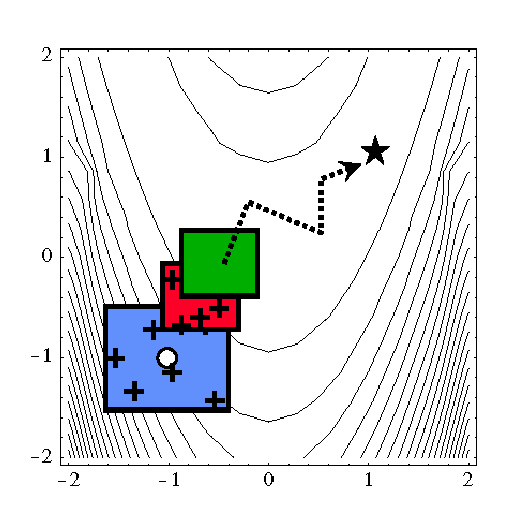
\includegraphics[width=.3\textwidth]{images/sbo_df}
  \caption{SBO iteration progression for global data fits.}
  \label{fig:sbo_df}
\end{wrapfigure}
When enforcing local consistency between a global data fit surrogate
and a high-fidelity model at a point, care must be taken to balance
this local consistency requirement with the global accuracy of the
surrogate.  In particular, performing a correction on an existing
global data fit in order to enforce local consistency can skew the
data fit and destroy its global accuracy.  One approach for achieving
this balance is to include the consistency requirement within the data
fit process by constraining the global data fit calculation (e.g.,
using constrained linear least squares).  This allows the data fit to
satisfy the consistency requirement while still addressing global
accuracy with its remaining degrees of freedom.
% Use figure from Theresa's paper?  Use equations from notes?
Embedding the consistency within the data fit also reduces the
sampling requirements.  For example, a quadratic polynomial normally
requires at least $(n+1)(n+2)/2$ samples for $n$ variables to perform
the fit.  However, with an embedded first-order consistency constraint
at a single point, the minimum number of samples is reduced by $n+1$ 
to $(n^2+n)/2$.
% With gradient information in each sample, this can be further
% reduced to ceil(n+2/2) samples.
%This corresponds to defining the terms of a symmetric Hessian matrix
%and points to an alternate approach.  Rather than enforcing
%consistency through constrained least squares, one can embed
%consistency directly by employing a Taylor series centered at the
%point of local consistency enforcement and globally estimating the
%higher order terms.  In the quadratic polynomial example, a
%second-order Taylor series with globally estimated Hessian terms
%requires the same $(n^2+n)/2$ samples and directly satisfies
%first-order consistency.  To further reduce sampling requirements in
%this case, one can choose to perform only partial updates (e.g., the
%diagonal) of the Hessian matrix~\cite{Per02}.

% Additional research area: Exploiting variance estimators to guide
% global search (e.g., kriging)

In the local and multipoint data fit cases, the iteration progression
will appear as in Fig.~\ref{fig:sbo_mh}.  Both cases involve a single
new evaluation of the original high-fidelity model per trust region,
with the distinction that multipoint approximations reuse information
from previous SBO iterates.  Like model hierarchy surrogates, these
techniques scale to larger numbers of design variables.  Unlike model
hierarchy surrogates, they generally do not require surrogate
corrections, since the matching conditions are embedded in the
surrogate form (as discussed for the global Taylor series approach
above).  The primary disadvantage to these surrogates is that the
region of accuracy tends to be smaller than for global data fits and
multifidelity surrogates, requiring more SBO cycles with smaller trust
regions.
%In SBO with surface fit functions, a sequence of optimization
%subproblems are evaluated, each of which is confined to a subset of
%the parameter space known as a ``trust region.'' Inside each trust
%region, Dakota's data sampling methods are used to evaluate the
%response quantities at a small number (order $10^{1}$ to $10^{2}$) of
%design points. Next, multidimensional surface fitting is performed to
%create a surrogate function for each of the response quantities.
%Finally, optimization is performed using the surrogate functions in
%lieu of the actual response quantities, and the optimizer's search is
%limited to the region inside the trust region bounds. A validation
%procedure is then applied to compare the predicted improvement in the
%response quantities to the actual improvement in the response
%quantities. Based on the results of this validation, the optimum
%design point is either accepted or rejected and the size of the trust
%region is either expanded, contracted, or left unchanged. The sequence
%of optimization subproblems continues until the SBO strategy
%convergence criteria are satisfied
More information on the design of experiments methods is available in
Chapter~\ref{dace}, and the data fit surrogates are described in
Section~\ref{models:surrogate:datafit}.

Figure~\ref{sbm:sblm_rosen} shows a Dakota input file that implements
surrogate-based optimization on Rosenbrock's function.
The first method keyword block contains the SBO 
keyword \texttt{surrogate\_based\_local}, plus the commands for
specifying the trust region size and scaling factors. The optimization
portion of SBO, using the CONMIN Fletcher-Reeves conjugate gradient method,
is specified in the following keyword blocks for
\texttt{method}, \texttt{model}, \texttt{variables}, and
\texttt{responses}.  The model used by the optimization method 
specifies that a global surrogate will be used to map variables into
responses (no \texttt{interface} specification is used by the
surrogate model). The global surrogate is constructed using a DACE
method which is identified with the \texttt{`SAMPLING'} identifier.
This data sampling portion of SBO is specified in the final set of
keyword blocks for \texttt{method}, \texttt{model},
\texttt{interface}, and \texttt{responses} (the earlier 
\texttt{variables} specification is reused). This example problem uses 
the Latin hypercube sampling method in the LHS software to select 10
design points in each trust region. A single surrogate model is
constructed for the objective function using a quadratic polynomial.
The initial trust region is centered at the design point
$(x_1,x_2)=(-1.2,1.0)$, and extends $\pm 0.4$ (10\% of the global
bounds) from this point in the $x_1$ and $x_2$ coordinate directions.
\begin{figure}
  \begin{bigbox}
    \begin{tiny}
      \verbatimtabinput[8]{rosen_opt_sbo.in}
    \end{tiny}
  \end{bigbox}
  \caption{Dakota input file for the surrogate-based local optimization
    example --
see \texttt{Dakota/examples/users/rosen\_opt\_sbo.in} }
  \label{sbm:sblm_rosen}
\end{figure}

If this input file is executed in Dakota, it will converge to the
optimal design point at $(x_{1},x_{2})=(1,1)$ in approximately 800
function evaluations. While this solution is correct, it is obtained
at a much higher cost than a traditional gradient-based optimizer
(e.g., see the results obtained in Section~\ref{tutorial:examples:optimization}).
This demonstrates that the SBO method with global data fits is not
really intended for use with smooth continuous optimization problems;
direct gradient-based optimization can be more efficient for such
applications. Rather, SBO with global data fits is best-suited for the
types of problems that occur in engineering design where the response
quantities may be discontinuous, nonsmooth, or may have multiple local
optima~\cite{Giu02}. In these types of engineering design problems,
traditional gradient-based optimizers often are ineffective, whereas
global data fits can extract the global trends of interest despite the
presence of local nonsmoothness (for an example problem with multiple
local optima, look in \texttt{Dakota/test} for the file
\texttt{dakota\_sbo\_sine\_fcn.in}~\cite{Giu00}).

The surrogate-based local minimizer is only mathematically
guaranteed to find a local minimum. However, in practice, SBO can often find 
the global minimum.  Due to the random sampling method used within the
SBO algorithm, the SBO method will solve a given problem a little differently 
each time it is run (unless the user specifies a particular random
number seed in the dakota input file as is shown in Figure~\ref{sbm:sblm_rosen}). 
Our experience on the quasi-sine function mentioned above is that if 
you run this problem 10 times with the same starting conditions but different 
seeds, then you will find the global minimum in about 70-80\% of the trials.
This is good performance for what is mathematically only a local optimization method.

\subsection{SBO with Multifidelity Models}\label{sbm:sblm:multifidelity}

When performing SBO with model hierarchies, the low-fidelity model is
normally fixed, requiring only a single high-fidelity evaluation to
compute a new correction for each new trust region.
Figure~\ref{fig:sbo_mh} displays this case.  This renders the
multifidelity SBO technique more scalable to larger numbers of design
variables since the number of high-fidelity evaluations per iteration
(assuming no finite differencing for derivatives) is independent of
the scale of the design problem.  However, the ability to smooth
poorly-behaved response variations in the high-fidelity model is lost,
and the technique becomes dependent on having a well-behaved
low-fidelity model\footnote{It is also possible to use a hybrid data
fit/multifidelity approach in which a smooth data fit of a noisy low
fidelity model is used in combination with a high fidelity model}.  In
addition, the parameterizations for the low and high-fidelity models
may differ, requiring the use of a mapping between these
parameterizations.  Space mapping, corrected space mapping, POD
mapping, and hybrid POD space mapping are being explored for this
purpose~\cite{Rob06a,Rob06b}.

\begin{wrapfigure}{r}{.3\textwidth}
  \centering
  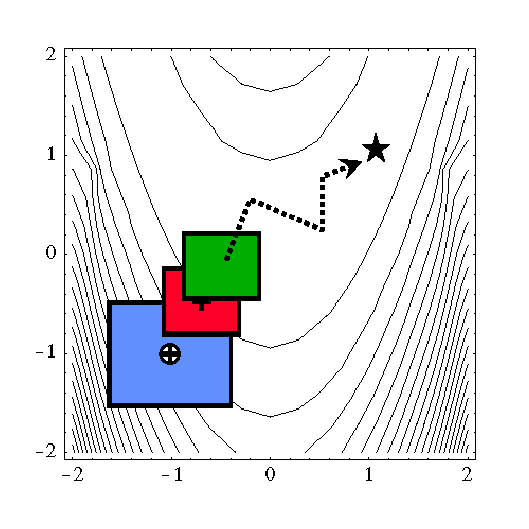
\includegraphics[width=.3\textwidth]{images/sbo_mh}
  \caption{SBO iteration progression for model hierarchies.}
  \label{fig:sbo_mh}
\end{wrapfigure}
%\begin{figure}
%\epsfxsize 3in
%\centerline{\epsfbox{sbo_mh.eps}}
%\caption{SBO iteration progression for model hierarchies.}
%\label{fig:sbo_mh}
%\end{figure}

When applying corrections to the low-fidelity model, there is no
concern for balancing global accuracy with the local consistency
requirements.  However, with only a single high-fidelity model evaluation
at the center of each trust region, it is critical to use the best
correction possible on the low-fidelity model in order to achieve
rapid convergence rates to the optimum of the high-fidelity
model~\cite{Eld04}.

%SBO can also be applied with multifidelity, or hierarchical, models,
%i.e., where one has available both a high-fidelity computational model
%and a low-fidelity computational model. This situation can occur when
%the low-fidelity model neglects some physical phenomena (e.g.,
%viscosity, heat transfer, etc.) that are included in the high-fidelity
%model, or when the low-fidelity model has a lower resolution
%computational mesh than the high-fidelity model. In many cases, the
%low-fidelity model can serve as a surrogate for the high-fidelity
%model during the optimization process. Thus, the low-fidelity model
%can be used in SBO in a manner similar to the use of surface fit
%models described in Section~\ref{sbm:sblm:surface}. A key difference
%in SBO with hierarchical surrogates is that a design of experiments
%using the high-fidelity model is not required; rather high-fidelity
%evaluations are only needed at the center of the current trust-region
%and the predicted optimum point in order to correct the low-fidelity
%model and verify improvement, respectively. Another difference is that
%one of the four types of correction described in
%Section~\ref{sbm:sblm:surface} is required for SBO with multifidelity
%models.

A multifidelity test problem named
\texttt{dakota\_sbo\_hierarchical.in} is available in
\texttt{Dakota/test} to demonstrate this SBO approach. This test
problem uses the Rosenbrock function as the high fidelity model and a
function named ``lf\_rosenbrock'' as the low fidelity model. Here,
lf\_rosenbrock is a variant of the Rosenbrock function (see
\texttt{Dakota\_Source/test/lf\_rosenbrock.C} for formulation) with the
minimum point at $(x_1,x_2)=(0.80,0.44)$, whereas the minimum of the
original Rosenbrock function is $(x_1,x_2)=(1,1)$. Multifidelity SBO
locates the high-fidelity minimum in 11 high fidelity evaluations for
additive second-order corrections and in 208 high fidelity evaluations
for additive first-order corrections, but fails for zeroth-order
additive corrections by converging to the low-fidelity minimum.

\subsection{SBO with Reduced Order Models}\label{sbm:sblm:rom}

When performing SBO with reduced-order models (ROMs), the ROM is
mathematically generated from the high-fidelity model.  A critical
issue in this ROM generation is the ability to capture the effect of
parametric changes within the ROM.  Two approaches to parametric ROM
are extended ROM (E-ROM) and spanning ROM (S-ROM)
techniques~\cite{Wei06}.  Closely related techniques include tensor
singular value decomposition (SVD) methods~\cite{Lat00}.  In the
single-point and multipoint E-ROM cases, the SBO iteration can appear
as in Fig.~\ref{fig:sbo_mh}, whereas in the S-ROM, global E-ROM, and
tensor SVD cases, the SBO iteration will appear as in
Fig.~\ref{fig:sbo_df}.  In addition to the high-fidelity model
analysis requirements, procedures for updating the system matrices and
basis vectors are also required.

Relative to data fits and multifidelity models, ROMs have some
attractive advantages.  Compared to data fits such as regression-based
polynomial models, they are more physics-based and would be expected
to be more predictive (e.g., in extrapolating away from the immediate
data).  Compared to multifidelity models, ROMS may be more practical
in that they do not require multiple computational models or meshes
which are not always available.  The primary disadvantage is potential
invasiveness to the simulation code for projecting the system using
the reduced basis.


\section{Surrogate-Based Global Minimization}\label{sbm:sbgm}

Surrogate-based global minimization differs from the surrogate-based
local minimization approach discussed in the previous section in
several ways: it is not a trust-region approach; initially there is
one global surrogate constructed over a set of sample points and the
optimizer operates on that surrogate (as opposed to adaptively
selecting points and re-building a surrogate in each trust region);
and there is no guarantee of convergence.

The \texttt{surrogate\_based\_global} method was developed to address
two needs.  The first is the case where a user wishes to use existing
function evaluations or a fixed sample size (perhaps based on
computational cost and allocation of resources) to build a surrogate
once and optimize on it.  In this case (a single global optimization
on a surrogate model), the set of surrogate building points is
determined in advance as opposed to the trust-region local surrogate
optimization in which the number of ``true'' function evaluations
depends on the location and size of the trust region, the goodness of
the surrogate within the trust-region, and problem characteristics.

In the second \texttt{surrogate\_based\_global} use case, we want to
update the surrogate, but globally.  That is, we add points to the
sample set used to create the surrogate, rebuild the surrogate, and
then perform another global optimization on the new surrogate.  Thus,
surrogate-based global optimization can be used in an iterative
scheme.  In one iteration, minimizers of the surrogate model are
found, and a selected subset of these are passed to the next
iteration.  In the next iteration, these surrogate points are
evaluated with the ``truth'' model, and then added to the set of
points upon which the next surrogate is constructed.  This presents a
more accurate surrogate to the minimizer at each subsequent iteration,
presumably driving to optimality quickly.  Note that a global
surrogate is constructed using the same bounds in each iteration.
This approach has no guarantee of convergence.

The surrogate-based global method was originally designed for MOGA (a
multi-objective genetic algorithm).  Since genetic algorithms often
need thousands or tens of thousands of points to produce optimal or
near-optimal solutions, surrogates can help by reducing the necessary
truth model evaluations.  Instead of creating one set of surrogates
for the individual objectives and running the optimization algorithm
on the surrogate once, the idea is to select points along the
(surrogate) Pareto frontier, which can be used to supplement the
existing points.  In this way, one does not need to use many points
initially to get a very accurate surrogate.  The surrogate becomes
more accurate as the iterations progress.

Most single objective optimization methods will return only a single
optimal point.  In that case, only one point from the surrogate model
will be evaluated with the ``true'' function and added to the pointset
upon which the surrogate is based.  In this case, it will take many
iterations of the surrogate-based global optimization for the approach
to converge, and its utility may not be as great as for the
multi-objective case when multiple optimal solutions are passed from
one iteration to the next to supplement the surrogate.  Note that the
user has the option of appending the optimal points from the surrogate
model to the current set of truth points or using the optimal points
from the surrogate model to replace the optimal set of points from the
previous iteration.  Although appending to the set is the default
behavior, at this time we strongly recommend using the option
\texttt{replace\_points} because it appears to be more accurate and
robust.

When using the surrogate-based global method, we first recommend
running one optimization on a single surrogate model. That is, set
\texttt{max\_iterations} to 1.  This will allow one to get a sense of
where the optima are located and also what surrogate types are the
most accurate to use for the problem.  Note that by fixing the seed of
the sample on which the surrogate is built, one can take a Dakota
input file, change the surrogate type, and re-run the problem without
any additional function evaluations by specifying the use of the
dakota restart file which will pick up the existing function
evaluations, create the new surrogate type, and run the optimization
on that new surrogate.  Also note that one can specify that surrogates
be built for all primary functions and constraints or for only a
subset of these functions and constraints.  This allows one to use a
"truth" model directly for some of the response functions, perhaps due
to them being much less expensive than other functions.  Finally, a
diagnostic threshold can be used to stop the method if the surrogate
is so poor that it is unlikely to provide useful points.  If the
goodness-of-fit has an R-squared value less than 0.5, meaning that
less than half the variance of the output can be explained or
accounted for by the surrogate model, the surrogate-based global
optimization stops and outputs an error message.  This is an arbitrary
threshold, but generally one would want to have an R-squared value as
close to 1.0 as possible, and an R-squared value below 0.5 indicates a
very poor fit.

For the surrogate-based global method, we initially recommend a small
number of maximum iterations, such as 3--5, to get a sense of how the
optimization is evolving as the surrogate gets updated globally.  If
it appears to be changing significantly, then a larger number (used in
combination with restart) may be needed.

Figure~\ref{sbm:sbgm_moga} shows a Dakota input file that implements
surrogate-based global optimization on a multi-objective test function. 
The first method keyword block contains the
keyword \texttt{surrogate\_based\_global}, plus the commands for
specifying five as the maximum iterations and the option to replace 
points in the global surrogate construction. The method block identified 
as MOGA specifies a multi-objective genetic algorithm optimizer and its 
controls.  The model keyword block specifies a surrogate model.  
In this case, a \texttt{gaussian\_process} model is used as a surrogate. 
The \texttt{dace\_method\_pointer} specifies that the surrogate will be 
build on 100 Latin Hypercube samples with a seed = 531.
The remainder of the input specification deals with the interface 
to the actual analysis driver and the 2 responses being returned 
as objective functions from that driver. 

\begin{figure}
  \begin{bigbox}
    \begin{scriptsize}
      \verbatimtabinput[8]{mogatest1_opt_sbo.in}
    \end{scriptsize}
  \end{bigbox}
  \caption{MOGA example -- 
see \texttt{Dakota/examples/users/mogatest1\_opt\_sbo.in} }
  \label{sbm:sbgm_moga}
\end{figure}
 
\section{Efficient Global Minimization}\label{sbm:egm}

Efficient Global Optimization (EGO) is a global optimization technique
that employs response surface surrogates~\cite{Jon98,Hua06}.  In each
EGO iteration, a Gaussian process (GP) approximation for the objective
function is constructed based on sample points of the true simulation.
The GP allows one to specify the prediction at a new input location as
well as the uncertainty associated with that prediction.  The key idea
in EGO is to maximize an Expected Improvement Function (EIF), defined
as the expectation that any point in the search space will provide a
better solution than the current best solution, based on the expected
values and variances predicted by the GP model.  It is important to
understand how the use of this EIF leads to optimal solutions.  The
EIF indicates how much the objective function value at a new potential
location is expected to be less than the predicted value at the
current best solution.  Because the GP model provides a Gaussian
distribution at each predicted point, expectations can be calculated.
Points with good expected values and even a small variance will have a
significant expectation of producing a better solution (exploitation),
but so will points that have relatively poor expected values and
greater variance (exploration).  The EIF incorporates both the idea of
choosing points which minimize the objective and choosing points about
which there is large prediction uncertainty (e.g., there are few or no
samples in that area of the space, and thus the probability may be
high that a sample value is potentially lower than other values).
Because the uncertainty is higher in regions of the design space with
few observations, this provides a balance between exploiting areas of
the design space that predict good solutions, and exploring areas
where more information is needed.

There are two major differences between our implementation and that of
~\cite{Jon98}: we do not use a branch and bound method to find points
which maximize the EIF.  Rather, we use the DIRECT algorithm.  Second,
we allow for multiobjective optimization and nonlinear least squares
including general nonlinear constraints.  Constraints are handled
through an augmented Lagrangian merit function approach (see
Surrogate-Based Minimization chapter in Dakota Theory
Manual~\cite{TheoMan}).

The method is specified as \texttt{efficient\_global}.  Currently we
do not expose any specification controls for the underlying Gaussian
process model used or for the optimization of the expected improvement
function, which is currently performed by the NCSU DIRECT
algorithm. The only item the user can specify is a seed which is 
used in the Latin Hypercube Sampling to generate the initial 
set of points which is used to construct the initial Gaussian process. 
An example specification for the EGO algorithm is shown in
Figure~\ref{sbm:egm_rosen}.
\begin{figure}
  \begin{bigbox}
    \begin{small}
      \verbatimtabinput[8]{rosen_opt_ego.in}
    \end{small}
  \end{bigbox}
  \caption{Dakota input file for the efficient global optimization example --
see \texttt{Dakota/examples/users/rosen\_opt\_ego.in} }
  \label{sbm:egm_rosen}
\end{figure}


\chapter{Advanced Strategies}\label{strat}

\section{Overview}\label{strat:overview}

DAKOTA's strategy capabilities were developed in order to provide a
control layer for managing multiple iterators and models. It was
driven by the observed need for ``meta-optimization'' and other high
level systems analysis procedures in real-world engineering design
problems. This capability allows the use of existing iterative
algorithm and computational model software components as building
blocks to accomplish more sophisticated studies, such as hybrid
minimization, multistart local minimization, Pareto optimization, or
mixed integer nonlinear programming (MINLP).  Other strategy-like
capabilities are enabled by the model recursion capabilities described
in Chapter~\ref{models}.  When these model recursion specifications
are sufficient to completely describe a multi-iterator, multi-model
solution approach, then a separate strategy specification is not used
(see Section~\ref{models:ex} for examples).  In addition, some
previous strategy capabilities (i.e., the surrogate-based minimization
approaches descibed in Chapter~\ref{sbm}) have migrated into the
method specification to allow their componentization and reuse
elsewhere.  This trend will continue in future releases with migration
of the MINLP strategy to the method specification, such that only the
most generic coordination approaches will remain.

\section{Hybrid Minimization}\label{strat:hybrid}

In the hybrid minimization strategy (keyword: \texttt{hybrid}), a
sequence of minimization methods are applied to find an optimal design
point. The goal of this strategy is to exploit the strengths of
different minimization algorithms through different stages of the
minimization process. Global/local optimization hybrids (e.g., genetic
algorithms combined with nonlinear programming) are a common example
in which the desire for a global optimum is balanced with the need for
efficient navigation to a local optimum. An important related feature
is that the sequence of minimization algorithms can employ models of
varying fidelity. In the global/local case, for example, it would
often be advantageous to use a low-fidelity model in the global search
phase, followed by use of a more refined model in the local search
phase.

The specification for hybrid minimization involves a list of
method identifier strings, and each of the corresponding method
specifications has the responsibility for identifying the model
specification (which may in turn identify variables, interface, and
responses specifications) that each method will use (see the DAKOTA
Reference Manual~\cite{RefMan} and the example discussed below).
Currently, only the sequential hybrid approach is available. The
\texttt{embedded} and \texttt{collaborative} approaches are
not fully functional at this time.

In the \texttt{sequential} hybrid minimization approach, a sequence
of minimization methods is invoked in the order specified in the
DAKOTA input file. In the default mode, 
the best solution from each method is used as the
starting point for the following method. If the user specifies
\texttt{num\_solutions\_transferred} and the method returns multiple 
optimal solutions (for example, with an evolutionary algorithm or DIRECT or 
a sampline method), then the specified number of solutions from the previous 
method will be used to initialize the subsequent method.  If the subsequent 
method cannot accept multiple input points (currently only a few methods 
such as the genetic algorithms in JEGA allow multiple input points), then 
multiple instances of the subsequent method are generated, each one 
initialized by one of the optimal solutions from the previous method. 
For example, if LHS sampling were run as the first method and 
the number of solutions transferred was 10 and the DOT conjugate gradient 
was the second method, there would be 10 instances of \texttt{dot\_frcg} 
started, each with a separate LHS sample solution as its initial point. 
Method switching is governed
by the separate convergence controls of each method; that is,
\emph{each method is allowed to run to its own internal definition of
completion without interference}. Individual method completion may be
determined by convergence criteria (e.g.,
\texttt{convergence\_tolerance}) or iteration limits (e.g.,
\texttt{max\_iterations}).  The \texttt{adaptive} option
is similar, with the difference that the progress of each method is
monitored and method switching is enforced according to
externally-defined relative progress metrics.  

%The \texttt{embedded} approach is restricted to special tightly-coupled
%hybrid algorithms in which local searches are used periodically to
%accelerate a global search.  These hybrids do not contain a discrete
%method switch, but rather repeatedly apply a local algorithm within
%the context of the global algorithm.

Figure~\ref{strat:figure01} shows a DAKOTA input file that specifies
a sequential hybrid optimization strategy to solve the
``textbook'' optimization test problem. This input file is named
\texttt{dakota\_hybrid.in} in the \texttt{Dakota/test} directory.
The three optimization methods are identified using the
\texttt{method\_list} specification in the strategy section of the
input file. The identifier strings listed in the specification are
`\texttt{GA}' for genetic algorithm, `\texttt{PS}' for pattern search,
and `\texttt{NLP}' for nonlinear programming. Following the strategy
keyword block are the three corresponding method keyword blocks. Note
that each method has a tag following the \texttt{id\_method} keyword
that corresponds to one of the method names listed in the strategy
keyword block. By following the identifier tags from \texttt{method}
to \texttt{model} and from \texttt{model} to \texttt{variables},
\texttt{interface}, and \texttt{responses}, it is easy to see the
specification linkages for this problem. The GA optimizer runs first
and uses model `\texttt{M1}' which includes variables `\texttt{V1}',
interface `\texttt{I1}', and responses `\texttt{R1}'. Once the GA is
complete, the PS optimizer starts from the best GA result and again
uses model `\texttt{M1}'. Since both GA and PS are nongradient-based
optimization methods, there is no need for gradient or Hessian
information in the `\texttt{R1}' response keyword block. The NLP
optimizer runs last, using the best result from the PS method as its
starting point.  It uses model `\texttt{M2}' which includes the same
`\texttt{V1}' and `\texttt{I1}' keyword blocks, but uses the responses
keyword block `\texttt{R2}' since the full Newton optimizer used in
this example (\texttt{optpp\_newton}) needs analytic gradient and
Hessian data to perform its search.
\begin{figure}
  \centering
  \begin{bigbox}
    \begin{tiny}
      \verbatimtabinput[8]{dakota_hybrid.in}
    \end{tiny}
  \end{bigbox}
  \caption{DAKOTA input file for a hybrid optimization strategy.}
  \label{strat:figure01}
\end{figure}

\section{Multistart Local Minimization}\label{strat:multistart}

A simple, heuristic, global minimization technique is to use many
local minimization runs, each of which is started from a different
initial point in the parameter space. This is known as multistart
local minimization. This is an attractive strategy in situations where
multiple local optima are known or expected to exist in the parameter
space. However, there is no theoretical guarantee that the global
optimum will be found. This approach combines the efficiency of local
minimization methods with a user-specified global stratification
(using a specified \texttt{starting\_points} list, a number of
specified \texttt{random\_starts}, or both; see the DAKOTA Reference
Manual~\cite{RefMan} for additional specification details). Since
solutions for different starting points are independent, parallel
computing may be used to concurrently run the local minimizations.

An example input file for multistart local optimization on the
``quasi\_sine'' test function (see \texttt{quasi\_sine\_fcn.C} in
\texttt{Dakota/test}) is shown in Figure~\ref{strat:figure02}. The
strategy keyword block in the input file contains the keyword
\texttt{multi\_start}, along with the set of starting points (3 random 
and 5 listed) that will be used for the optimization runs. The other
keyword blocks in the input file are similar to what would be used in
a single optimization run.

\begin{figure}
  \centering
  \begin{bigbox}
    \begin{small}
      \verbatimtabinput[8]{dakota_multistart.in}
    \end{small}
  \end{bigbox}
  \caption{DAKOTA input file for a multistart local optimization strategy.}
  \label{strat:figure02}
\end{figure}

The \texttt{quasi\_sine} test function has multiple local minima, but
there is an overall trend in the function that tends toward the global
minimum at $(x1,x2)=(0.177,0.177)$. See~\cite{Giu00} for more
information on this test function. Figure~\ref{strat:figure03} shows
the results summary for the eight local optimizations performed. From
the five specified starting points and the 3 random starting points
(as identified by the \texttt{x1}, \texttt{x2} headers), the eight
local optima (as identified by the \texttt{x1*},
\texttt{x2*} headers) are all different and only one of the local
optimizations finds the global minimum.

\begin{figure}
\centering
\begin{bigbox}
\begin{footnotesize}
\begin{verbatim}
<<<<< Results summary:
   set_id             x1             x2            x1*            x2*         obj_fn 
        1           -0.8           -0.8  -0.8543728666  -0.8543728666   0.5584096919 
        2           -0.8            0.8  -0.9998398719    0.177092822    0.291406596 
        3            0.8           -0.8    0.177092822  -0.9998398719    0.291406596 
        4            0.8            0.8   0.1770928217   0.1770928217   0.0602471946 
        5              0              0  0.03572926375  0.03572926375  0.08730499239 
        6  -0.7767971993  0.01810943539  -0.7024118387  0.03572951143   0.3165522387 
        7  -0.3291571008  -0.7697378755   0.3167607374  -0.4009188363   0.2471403213 
        8   0.8704730469   0.7720679005    0.177092899   0.3167611757  0.08256082751 
\end{verbatim}
\end{footnotesize}
\end{bigbox}
\caption{DAKOTA results summary for a multistart local optimization strategy.}
\label{strat:figure03}
\end{figure}

\section{Pareto Optimization}\label{strat:pareto}

The Pareto optimization strategy (keyword: \texttt{pareto\_set}) is
one of three multiobjective optimization capabilities discussed in
Section~\ref{opt:additional:multiobjective}. In the Pareto
optimization strategy, multiple sets of multiobjective weightings are
evaluated. The user can specify these weighting sets in the strategy
keyword block using a \texttt{multi\_objective\_weight\_sets} list, a
number of \texttt{random\_weight\_sets}, or both (see the DAKOTA
Reference Manual~\cite{RefMan} for additional specification details).
Figure~\ref{strat:figure04} shows the input commands from the file
\texttt{dakota\_pareto.in} in the \texttt{Dakota/test} directory.

DAKOTA performs one multiobjective optimization problem for each set
of multiobjective weights. The collection of computed optimal
solutions form a Pareto set, which can be useful in making trade-off
decisions in engineering design. Since solutions for different
multiobjective weights are independent, parallel computing may be used
to concurrently execute the multiobjective optimization problems.

Figure~\ref{strat:figure05} shows the results summary for the
Pareto-set optimization strategy. For the four multiobjective
weighting sets (as identified by the \texttt{w1}, \texttt{w2},
\texttt{w3} headers), the local optima (as identified by the
\texttt{x1}, \texttt{x2} headers) are all different and correspond to
individual objective function values of ($f_1,f_2,f_3$) =
(0.0,0.5,0.5), (13.1,-1.2,8.16), (532.,33.6,-2.9), and (0.125,0.0,0.0)
(note: the composite objective function is tabulated under the
\texttt{obj\_fn} header).  The first three solutions reflect exclusive
optimization of each of the individual objective functions in turn,
whereas the final solution reflects a balanced weighting and the
lowest sum of the three objectives.  Plotting these ($f_1,f_2,f_3$)
triplets on a 3-dimensional plot results in a Pareto surface (not
shown), which is useful for visualizing the trade-offs in the
competing objectives.

\begin{figure}
  \centering
  \begin{bigbox}
    \begin{small}
      \verbatimtabinput[8]{dakota_pareto.in}
    \end{small}
  \end{bigbox}
  \caption{DAKOTA input file for the Pareto optimization strategy.}
  \label{strat:figure04}
\end{figure}

\begin{figure}
\centering
\begin{bigbox}
\begin{scriptsize}
\begin{verbatim}
<<<<< Results summary:
   set_id             w1             w2             w3             x1             x2         obj_fn
        1              1              0              0   0.9996554048    0.997046351 7.612301561e-11
        2              0              1              0            0.5            2.9           -1.2
        3              0              0              1            5.8 1.12747589e-11           -2.9
        4          0.333          0.333          0.333            0.5   0.5000000041       0.041625
\end{verbatim}
\end{scriptsize}
\end{bigbox}
\caption{DAKOTA results summary for the Pareto-set optimization
  strategy.}
\label{strat:figure05}
\end{figure}

\section{Mixed Integer Nonlinear Programming (MINLP)}\label{strat:minlp}

\emph{For DAKOTA 5.1, branch and bound is currently inoperative due to 
ongoing restructuring of PICO and its incorporation into COLINY.
This will be supported again in future releases.}

Many nonlinear optimization problems involve a combination of discrete
and continuous variables. These are known as mixed integer nonlinear
programming (MINLP) problems. A typical MINLP optimization problem is
formulated as follows:

\begin{eqnarray}
  \hbox{minimize:} & & f(\mathbf{x,d})\nonumber\\
  \hbox{subject to:} & & \mathbf{g}_{L} \leq \mathbf{g(x,d)}
    \leq \mathbf{g}_{U}\nonumber\\
  & & \mathbf{h(x,d)}=\mathbf{h}_{t}\label{strat:equation01}\\
  & & \mathbf{x}_{L} \leq \mathbf{x} \leq \mathbf{x}_{U}\nonumber\\
  & & \mathbf{d} \in \{-2,-1,0,1,2\}\nonumber
\end{eqnarray}

where $\mathbf{d}$ is a vector whose elements are integer values. In
situations where the discrete variables can be temporarily relaxed
(i.e., noncategorical discrete variables, see
Section~\ref{variables:design:ddv}), the branch-and-bound
algorithm can be applied. Categorical variables (e.g., true/false
variables, feature counts, etc.) that are not relaxable cannot be used
with the branch and bound strategy.  During the branch and bound
process, the discrete variables are treated as continuous variables
and the integrality conditions on these variables are incrementally
enforced through a sequence of optimization subproblems.  By the end
of this process, an optimal solution that is feasible with respect to
the integrality conditions is computed.

DAKOTA's branch and bound strategy (keyword:
\texttt{branch\_and\_bound}) can solve optimization problems having
either discrete or mixed continuous/discrete variables. This strategy
uses the parallel branch-and-bound algorithm from the PICO software
package~\cite{Eck97,Eck01} to generate a series of optimization
subproblems (``branches''). These subproblems are solved as continuous
variable problems using any of DAKOTA's nonlinear optimization
algorithms (e.g., DOT, NPSOL). When a solution to a branch is feasible
with respect to the integrality constraints, it provides an upper
bound on the optimal objective function, which can be used to prune
branches with higher objective functions that are not yet
feasible. Since solutions for different branches are independent,
parallel computing may be used to concurrently execute the
optimization subproblems.

PICO, by itself, targets the solution of mixed integer linear
programming (MILP) problems, and through coupling with DAKOTA's
nonlinear optimizers, is extended to solution of MINLP problems. In
the case of MILP problems, the upper bound obtained with a feasible
solution is an exact bound and the branch and bound process is
provably convergent to the global minimum. For nonlinear problems
which may exhibit nonconvexity or multimodality, the process is
heuristic in general, since there may be good solutions that are
missed during the solution of a particular branch. However, the
process still computes a series of locally optimal solutions, and is
therefore a natural extension of the results from local optimization
techniques for continuous domains. Only with rigorous global
optimization of each branch can a global minimum be guaranteed when
performing branch and bound on nonlinear problems of unknown
structure.

In cases where there are only a few discrete variables and when the
discrete values are drawn from a small set, then it may be reasonable
to perform a separate optimization problem for all of the possible
combinations of the discrete variables. However, this brute force
approach becomes computationally intractable if these conditions are
not met. The branch-and-bound algorithm will generally require
solution of fewer subproblems than the brute force method, although it
will still be significantly more expensive than solving a purely
continuous design problem.

\subsection{Example MINLP Problem}\label{strat:minlp:example}

As an example, consider the following MINLP problem~\cite{Eld99}:

\begin{eqnarray}
  \hbox{minimize:} & &
  f(\mathbf{x})=\sum_{i=1}^{6}(x_{i}-1.4)^{4}\nonumber\\
  & & g_{1}=x_{1}^{2}-\frac{x_{2}}{2} \leq 0\nonumber\\
  & & g_{2}=x_{2}^{2}-\frac{x_{1}}{2} \leq 0\label{strat:equation02}\\
  & & -10 \leq x_{1},x_{2},x_{3},x_{4} \leq 10\nonumber\\
  & & x_{5},x_{6} \in \{0,1,2,3,4\}\nonumber
\end{eqnarray}

This problem is a variant of the textbook test problem described in
Section~\ref{additional:textbook}. In addition to the introduction of
two integer variables, a modified value of $1.4$ is used inside the
quartic sum to render the continuous solution a non-integral solution.
%Figure~\ref{strat:figure06} shows a DAKOTA input file for solving this
%problem. This input file is named \texttt{dakota\_bandb.in} in the
%\texttt{Dakota/test} directory. Note the specification for the
%discrete variables, where lower and upper bounds are given. The
%discrete variables can take on any integer value within these bounds.

%\begin{figure}
%  \centering
%  \begin{bigbox}
%    \begin{small}
%      \verbatimtabinput[8]{dakota_bandb.in}
%    \end{small}
%  \end{bigbox}
%  \caption{DAKOTA input file for the branch-and-bound strategy for
%    solving MINLP optimization problems.}
%  \label{strat:figure06}
%\end{figure}

Figure~\ref{strat:figure07} shows the sequence of branches generated
for this problem.  The first optimization subproblem relaxes the
integrality constraint on parameters $x_{5}$ and $x_{6}$, so that $0
\leq x_{5} \leq 4$ and $0 \leq x_{6} \leq 4$. The values for $x_{5}$
and $x_{6}$ at the solution to this first subproblem are
$x_{5}=x_{6}=1.4$.  Since $x_{5}$ and $x_{6}$ must be integers, the
next step in the solution process ``branches'' on parameter $x_{5}$ to
create two new optimization subproblems; one with $0 \leq x_{5} \leq
1$ and the other with $2 \leq x_{5} \leq 4$.  Note that, at this first
branching, the bounds on $x_{6}$ are still $0 \leq x_{6} \leq 4$.
Next, the two new optimization subproblems are solved.  Since they are
independent, they can be performed in parallel.  The branch-and-bound
process continues, operating on both $x_{5}$ and $x_{6}$ , until a
optimization subproblem is solved where $x_{5}$ and $x_{6}$ are
integer-valued. At the solution to this problem, the optimal values
for $x_{5}$ and $x_{6}$ are $x_{5}=x_{6}=1$.

\begin{figure}
  \centering
  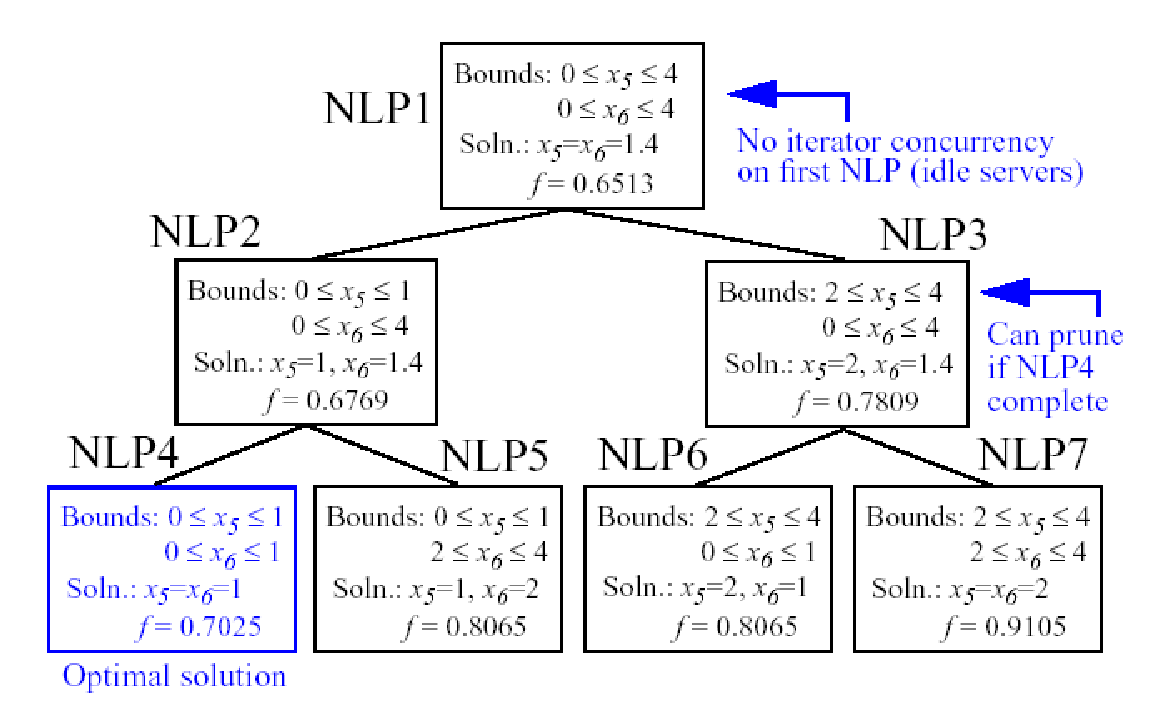
\includegraphics[scale=0.75]{images/branch_history}
  \caption{Branching history for example MINLP optimization problem.}
  \label{strat:figure07}
\end{figure}

In this example problem, the branch-and-bound algorithm executes as
few as five and no more than seven optimization subproblems to reach
the solution. For comparison, the brute force approach would require
25 optimization problems to be solved (i.e., five possible values for
each of $x_{5}$ and $x_{6}$ ).

%In the example given above, the discrete variables are integer-valued.
%In some cases, the discrete variables may be real-valued, such as $x
%\in \{0.0,0.5,1.0,1.5,2.0\}$.  The branch-and-bound algorithm is
%restricted to work with integer values. Therefore, it is up to the
%user to perform a transformation between the discrete integer values
%from DAKOTA and the discrete real values that are passed to the
%simulation code (see Section~\ref{variables:design:ddv}).  When
%integrality is not being relaxed, a common mapping is to use the
%integer value from DAKOTA as the index into a vector of discrete real
%values.  However, when integrality is relaxed, additional logic for
%interpolating between the discrete real values is needed.
% Note: it should be straightforward to extend MINLP to support
% general discrete variables, if PICO would support it.  Does this
% come up in MILP for logistics, etc.?

\chapter{Models}\label{models}

\section{Overview}\label{models:overview}

Chapters~\ref{ps} through~\ref{nls} presented the different
``iterators'' (or methods) available in Dakota.  An iterator iterates
on a model in order to map a set of variables into a set of responses.
This model may involve a simple mapping involving a single interface,
or it may involve recursions using sub-iterator and sub-models.  These
recursion capabilities were developed in order to provide mechanisms
for ``nesting,'' ``layering,'' and ``recasting'' of software
components, which allows the use of these components as building
blocks to accomplish more sophisticated studies, such as
surrogate-based optimization or optimization under uncertainty.  In a
nested relationship, a sub-iterator is executed using its sub-model
for every evaluation of the nested model.  In a layered relationship,
on the other hand, sub-iterators and sub-models are used only for
periodic updates and verifications.  And in a recast relationship, the
input variable and output response definitions in a sub-model are
reformulated in order to support new problem definitions.  In each of
these cases, the sub-model is of arbitrary type, such that model
recursions can be chained together in as long of a sequence as needed
(e.g., layered containing nested contained layered containing single
in Section~\ref{adv_models:ouu:sb}).  Figure~\ref{model:hier} displays
the model class hierarchy from the Dakota Developers
Manual~\cite{DevMan}, with derived classes for single models, nested
models, recast models, and two types of surrogate models: data fit and
hierarchical/multifidelity.  A third type of derived surrogate model
supporting reduced-order models (ROM) is planned for future releases.

\begin{figure}
  \centering 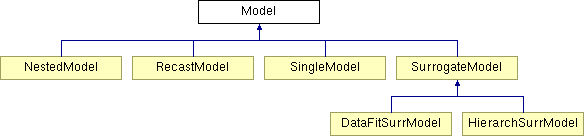
\includegraphics[scale=0.65]{images/classDakota_1_1Model}
  \caption{The Dakota model class hierarchy.}  \label{model:hier}
\end{figure}

Section~\ref{models:single} describes single models;
Section~\ref{models:recast} describes recast models;
Section~\ref{models:surrogate} describes surrogate models of the data
fit, multifidelity, and ROM type; and Section~\ref{models:nested}
describes nested models.  Finally, Chapter~\ref{adv_models} presents
a number of advanced examples demonstrating these model recursions.

\section{Single Models}\label{models:single}

The single model is the simplest model type.  It uses a single
interface instance (see Chapter~\ref{interfaces}) to map variables
(see Chapter~\ref{variables}) into responses (see
Chapter~\ref{responses}).  There is no recursion in this case.  Refer
to the Models chapter in the Dakota Reference Manual~\cite{RefMan} for
additional information on the single model specification.

\section{Recast Models}\label{models:recast}

The recast model is not directly visible to the user within the input
specification.  Rather, it is used ``behind the scenes'' to recast the
inputs and outputs of a sub-model for the purposes of reformulating
the problem posed to an iterator.  Examples include variable and
response scaling (see Section~\ref{opt:additional:scaling}),
transformations of uncertain variables and associated response
derivatives to employ standardized random variables (see
Sections~\ref{uq:reliability} and~\ref{uq:expansion}), multiobjective
optimization (see Section~\ref{opt:additional:multiobjective}), merit
functions (see Section~\ref{sbm:sblm}), and expected
improvement/feasibility (see Sections~\ref{sbm:egm}
and~\ref{uq:reliability:global}).  Refer to the Dakota Developers
Manual~\cite{DevMan} for additional details on the mechanics of
recasting problem formulations.

\section{Surrogate Models}\label{models:surrogate}

Surrogate models are inexpensive approximate models that are intended
to capture the salient features of an expensive high-fidelity model.
They can be used to explore the variations in response quantities over
regions of the parameter space, or they can serve as inexpensive
stand-ins for optimization or uncertainty quantification studies (see,
for example, the surrogate-based optimization strategy in
Section~\ref{sbm}).  Surrogate models supported in Dakota can be
categorized into three types: data fits, multifidelity, and
reduced-order model surrogates.  An overview and discussion of
surrogate correction is provided here, with details following.

\subsection{Overview of Surrogate Types}


Data fitting methods involve construction of an approximation or
surrogate model using data (response values, gradients, and Hessians)
generated from the original truth model.  Data fit methods can be
further categorized as local, multipoint, and global approximation
techniques, based on the number of points used in generating the data
fit.  Local methods involve response data from a single point in
parameter space.  Available local techniques currently include:

\textbf{Taylor Series Expansion}: This is a local first-order or
second-order expansion centered at a single point in the parameter space.

Multipoint approximations involve response data from two or more
points in parameter space, often involving the current and previous
iterates of a minimization algorithm.  Available techniques currently
include:

\textbf{TANA-3}: This multipoint approximation uses a two-point
exponential approximation~\cite{Xu98,Fad90} built with response value
and gradient information from the current and previous iterates.

Global methods, often referred to as \emph{response surface methods},
involve many points spread over the parameter ranges of interest.
These surface fitting methods work in conjunction with the sampling
methods and design of experiments methods described in
Section~\ref{capabilities:sampling}.

\textbf{Polynomial Regression}: First-order (linear), second-order
(quadratic), and third-order (cubic) polynomial response surfaces
computed using linear least squares regression methods. Note: there is
currently no use of forward- or backward-stepping regression methods
to eliminate unnecessary terms from the polynomial model.

\textbf{Gaussian Process (GP) or Kriging Interpolation}
Dakota contains two implementations of Gaussian process, also known as 
Kriging ~\cite{Giu98}, spatial interpolation.  One of these resides in 
the Surfpack sub-package of Dakota, the other resides in Dakota itself.
Both versions use the Gaussian correlation function with parameters that
are selected by Maximum Likelihood Estimation (MLE). This correlation 
function results in a response surface that is $C^\infty$-continuous.
Prior to Dakota 5.2, the Surfpack GP was referred to as the ``Kriging'' 
model and the Dakota version was labeled as the ``Gaussian Process.''  
These terms are now used interchangeably.  As of Dakota 5.2,the 
Surfpack GP is used by default.  For now the user still has the option 
to select the Dakota GP, but the Dakota GP is deprecated and will be 
removed in a future release.
\begin{itemize}
\item \textbf{Surfpack GP}: Ill-conditioning due to a poorly spaced sample 
      design is handled by discarding points that contribute the least 
      unique information to the correlation matrix.  Therefore, the points 
      that are discarded are the ones that are easiest to predict.  The 
      resulting surface will exactly interpolate the data values at the 
      retained points but is not guaranteed to interpolate the discarded 
      points.
\item \textbf{Dakota GP}: Ill-conditioning is handled by adding a jitter 
      term or ``nugget'' to diagonal elements of the correlation matrix. 
      When this happens, the Dakota GP may not exactly interpolate the 
      data values.
\end{itemize}

\textbf{Artificial Neural Networks}: An implementation of the
stochastic layered perceptron neural network developed by Prof. D. C.
Zimmerman of the University of Houston~\cite{Zim96}. This neural network
method is intended to have a lower training (fitting) cost than
typical back-propagation neural networks.

\textbf{Multivariate Adaptive Regression Splines (MARS)}: Software
developed by Prof. J. H. Friedman of Stanford University~\cite{Fri91}.
The MARS method creates a $C^2$-continuous patchwork of splines in the
parameter space.

\textbf{Radial Basis Functions (RBF)}:  Radial basis functions are 
functions whose value typically depends on the distance from a center point, 
called the centroid.  The surrogate model approximation is constructed
as the weighted sum of individual radial basis functions. 

\textbf{Moving Least Squares (MLS)}: Moving Least Squares can be 
considered a more specialized version of linear regression models.
MLS is a weighted least squares approach where the weighting is 
``moved'' or recalculated for every new point where 
a prediction is desired.~\cite{Nea04} 

%\textbf{Orthogonal Polynomials}: This technique involves the use of
%multivariate orthogonal polynomials as a global basis for surrogate
%modeling.  These multivariate polynomials are constructed as a product
%of particular univariate orthogonal polynomials, including Hermite,
%Legendre, Laguerre, Jacobi, and generalized Laguerre polynomials,
%which are defined as functions of standard normal, standard uniform,
%standard exponential, standard beta, and standard gamma random
%variables, respectively.  Given the probabilistic interpretation of
%the approximation variables, this data fit is primarily used for
%uncertainty quantification, and in particular, polynomial chaos
%expansions.

In addition to data fit surrogates, Dakota supports multifidelity 
and reduced-order model approximations:

\textbf{Multifidelity Surrogates}: Multifidelity modeling involves the
use of a low-fidelity physics-based model as a surrogate for the
original high-fidelity model.  The low-fidelity model typically
involves a coarser mesh, looser convergence tolerances, reduced
element order, or omitted physics.  It is a separate model in its own
right and does not require data from the high-fidelity model for
construction.  Rather, the primary need for high-fidelity evaluations
is for defining correction functions that are applied to the
low-fidelity results.

\textbf{Reduced Order Models}: A reduced-order model (ROM) is
mathematically derived from a high-fidelity model using the technique
of Galerkin projection.  By computing a set of basis functions (e.g.,
eigenmodes, left singular vectors) that capture the principal dynamics
of a system, the original high-order system can be projected to a much
smaller system, of the size of the number of retained basis functions.

\subsection{Correction Approaches}

Each of the surrogate model types supports the use of correction
factors that improve the local accuracy of the surrogate models. The
correction factors force the surrogate models to match the true
function values and possibly true function derivatives at the center
point of each trust region. Currently, Dakota supports either zeroth-,
first-, or second-order accurate correction methods, each of which can
be applied using either an additive, multiplicative, or combined
correction function. For each of these correction approaches, the
correction is applied to the surrogate model and the corrected model
is then interfaced with whatever algorithm is being employed.  The
default behavior is that no correction factor is applied.

The simplest correction approaches are those that enforce consistency
in function values between the surrogate and original models at a
single point in parameter space through use of a simple scalar offset
or scaling applied to the surrogate model.  First-order corrections
such as the first-order multiplicative correction (also known as beta
correction~\cite{Cha93}) and the first-order additive
correction~\cite{Lew00} also enforce consistency in the gradients and
provide a much more substantial correction capability that is
sufficient for ensuring provable convergence in SBO algorithms (see
Section~\ref{sbm:sblm}).  SBO convergence rates can be further
accelerated through the use of second-order corrections which also
enforce consistency in the Hessians~\cite{Eld04}, where the
second-order information may involve analytic, finite-difference, or
quasi-Newton Hessians.

Correcting surrogate models with additive corrections involves
\begin{equation}
\hat{f_{hi_{\alpha}}}({\bf x}) = f_{lo}({\bf x}) + \alpha({\bf x}) 
\label{eq:correct_val_add}
\end{equation}
where multifidelity notation has been adopted for clarity.  For
multiplicative approaches, corrections take the form
\begin{equation}
\hat{f_{hi_{\beta}}}({\bf x}) = f_{lo}({\bf x}) \beta({\bf x})
\label{eq:correct_val_mult}
\end{equation}
where, for local corrections, $\alpha({\bf x})$ and $\beta({\bf x})$
are first or second-order Taylor series approximations to the exact
correction functions:
\begin{eqnarray}
\alpha({\bf x}) & = & A({\bf x_c}) + \nabla A({\bf x_c})^T 
({\bf x} - {\bf x_c}) + \frac{1}{2} ({\bf x} - {\bf x_c})^T 
\nabla^2 A({\bf x_c}) ({\bf x} - {\bf x_c}) \label{eq:taylor_a} \\
\beta({\bf x})  & = & B({\bf x_c}) + \nabla B({\bf x_c})^T 
({\bf x} - {\bf x_c}) + \frac{1}{2} ({\bf x} - {\bf x_c})^T \nabla^2 
B({\bf x_c}) ({\bf x} - {\bf x_c}) \label{eq:taylor_b}
\end{eqnarray}
where the exact correction functions are
\begin{eqnarray}
A({\bf x}) & = & f_{hi}({\bf x}) - f_{lo}({\bf x})       \label{eq:exact_A} \\
B({\bf x}) & = & \frac{f_{hi}({\bf x})}{f_{lo}({\bf x})} \label{eq:exact_B}
\end{eqnarray}
Refer to \cite{Eld04} for additional details on the derivations.

A combination of additive and multiplicative corrections can provide
for additional flexibility in minimizing the impact of the correction
away from the trust region center.  In other words, both additive and
multiplicative corrections can satisfy local consistency, but through
the combination, global accuracy can be addressed as well.  This
involves a convex combination of the additive and multiplicative
corrections:
\begin{equation}
\hat{f_{hi_{\gamma}}}({\bf x}) = \gamma \hat{f_{hi_{\alpha}}}({\bf x}) +
(1 - \gamma) \hat{f_{hi_{\beta}}}({\bf x}) \label{eq:combined_form}
\end{equation}
where $\gamma$ is calculated to satisfy an additional matching
condition, such as matching values at the previous design iterate.

%It should be noted that in both first order correction methods, the
%function $\hat{f}(x)$ matches the function value and gradients of
%$f_{t}(x)$ at $x=x_{c}$. This property is necessary in proving that
%the first order-corrected SBO algorithms are provably convergent to a
%local minimum of $f_{t}(x)$.  However, the first order correction
%methods are significantly more expensive than the zeroth order
%correction methods, since the first order methods require computing
%both $\nabla f_{t}(x_{c})$ and $\nabla f_{s}(x_{c})$.  When the SBO
%strategy is used with either of the zeroth order correction methods,
%or with no correction method, convergence is not guaranteed to a local
%minimum of $f_{t}(x)$. That is, the SBO strategy becomes a heuristic
%optimization algorithm. From a mathematical point of view this is
%undesirable, but as a practical matter, the heuristic variants of SBO
%are often effective in finding local minima.

%\emph{Usage guidelines:}
%\begin{itemize}
%\item Both the \texttt{additive zeroth\_order} and
%  \texttt{multiplicative zeroth\_order} correction methods are
%  ``free'' since they use values of $f_{t}(x_{c})$ that are normally
%  computed by the SBO strategy.
%
%\item The use of either the \texttt{additive first\_order} method or
%  the \texttt{multiplicative first\_order} method does not necessarily
%  improve the rate of convergence of the SBO algorithm.
%
%\item When using the first order correction methods, the
%  \texttt{TRUE\_FCN\_GRAD} response keywords must be modified (see
%  bottom of Figure~\ref{sbm:sblm_rosen}) to allow either analytic or
%  numerical gradients to be computed. This provides the gradient data
%  needed to compute the correction function.
%
%\item For many computationally expensive engineering optimization
%  problems, gradients often are too expensive to obtain or are
%  discontinuous (or may not exist at all). In such cases the heuristic
%  SBO algorithm has been an effective approach at identifying optimal
%  designs~\cite{Giu02}.
%\end{itemize}

\subsection{Data Fit Surrogate Models}\label{models:surrogate:datafit}

A surrogate of the {\em data fit} type is a non-physics-based
approximation typically involving interpolation or regression of a set
of data generated from the original model.  Data fit surrogates can be
further characterized by the number of data points used in the fit,
where a local approximation (e.g., first or second-order Taylor
series) uses data from a single point, a multipoint approximation
(e.g., two-point exponential approximations (TPEA) or two-point
adaptive nonlinearity approximations (TANA)) uses a small number of
data points often drawn from the previous iterates of a particular
algorithm, and a global approximation (e.g., polynomial response
surfaces, kriging/gaussian\_process, neural networks, radial basis 
functions, splines)
uses a set of data points distributed over the domain of interest,
often generated using a design of computer experiments.

Dakota contains several types of surface fitting methods that can be
used with optimization and uncertainty quantification methods and
strategies such as surrogate-based optimization and optimization under
uncertainty. These are: polynomial models (linear, quadratic, and
cubic), first-order Taylor series expansion, kriging spatial
interpolation, artificial neural networks, multivariate adaptive
regression splines, radial basis functions, and moving least squares. 
With the exception of Taylor series methods, all of the above methods 
listed in the previous sentence are accessed in Dakota through the 
Surfpack library.  All of these surface fitting methods can be
applied to problems having an arbitrary number of design parameters.
However, surface fitting methods usually are practical only for
problems where there are a small number of parameters (e.g., a maximum
of somewhere in the range of 30-50 design parameters). The
mathematical models created by surface fitting methods have a variety
of names in the engineering community. These include surrogate models,
meta-models, approximation models, and response surfaces. For this
manual, the terms surface fit model and surrogate model are used.

The data fitting methods in Dakota include software developed by
Sandia researchers and by various researchers in the academic
community.

\subsubsection{Procedures for Surface Fitting}\label{models:surf:procedures}

The surface fitting process consists of three steps: (1) selection of
a set of design points, (2) evaluation of the true response quantities
(e.g., from a user-supplied simulation code) at these design points,
and (3) using the response data to solve for the unknown coefficients
(e.g., polynomial coefficients, neural network weights, kriging
correlation factors) in the surface fit model. In cases where there is
more than one response quantity (e.g., an objective function plus one
or more constraints), then a separate surface is built for each
response quantity. Currently, the surface fit models are built using
only 0$^{\mathrm{th}}$-order information (function values only), although
extensions to using higher-order information (gradients and Hessians)
are possible. Each surface fitting method employs a different
numerical method for computing its internal coefficients. For example,
the polynomial surface uses a least-squares approach that employs a
singular value decomposition to compute the polynomial coefficients,
whereas the kriging surface uses Maximum Likelihood Estimation to
compute its correlation coefficients. More information on the
numerical methods used in the surface fitting codes is provided in the
Dakota Developers Manual~\cite{DevMan}.

The set of design points that is used to construct a surface fit model
is generated using either the DDACE software package~\cite{TonXX} or the
LHS software package~\cite{Ima84}. These packages provide a variety of
sampling methods including Monte Carlo (random) sampling, Latin
hypercube sampling, orthogonal array sampling, central composite
design sampling, and Box-Behnken sampling. More information on these
software packages is provided in Chapter~\ref{dace}.

\subsubsection{Taylor Series}\label{models:surf:taylor}

The Taylor series model is purely a local approximation method. That
is, it provides local trends in the vicinity of a single point in
parameter space. The first-order Taylor series expansion is:
\begin{equation}
\hat{f}({\bf x}) \approx f({\bf x}_0) + \nabla_{\bf x} f({\bf x}_0)^T 
({\bf x} - {\bf x}_0) \label{eq:taylor1}
\end{equation}
and the second-order expansion is:
\begin{equation}
\hat{f}({\bf x}) \approx f({\bf x}_0) + \nabla_{\bf x} f({\bf x}_0)^T 
({\bf x} - {\bf x}_0) + \frac{1}{2} ({\bf x} - {\bf x}_0)^T 
\nabla^2_{\bf x} f({\bf x}_0) ({\bf x} - {\bf x}_0) \label{eq:taylor2}
\end{equation}

where ${\bf x}_0$ is the expansion point in $n$-dimensional parameter
space and $f({\bf x}_0)$, $\nabla_{\bf x} f({\bf x}_0)$, and
$\nabla^2_{\bf x} f({\bf x}_0)$ are the computed response value,
gradient, and Hessian at the expansion point, respectively.  As
dictated by the responses specification used in building the local
surrogate, the gradient may be analytic or numerical and the Hessian
may be analytic, numerical, or based on quasi-Newton secant updates.

In general, the Taylor series model is accurate only in the region of
parameter space that is close to ${\bf x}_0$ . While the accuracy is
limited, the first-order Taylor series model reproduces the correct
value and gradient at the point $\mathbf{x}_{0}$, and the second-order
Taylor series model reproduces the correct value, gradient, and
Hessian. This consistency is useful in provably-convergent
surrogate-based optimization. The other surface fitting methods do not
use gradient information directly in their models, and these methods
rely on an external correction procedure in order to satisfy the
consistency requirements of provably-convergent SBO.

\subsubsection{Two Point Adaptive Nonlinearity Approximation}\label{models:surf:tana}

The TANA-3 method~\cite{Xu98} is a multipoint approximation method
based on the two point exponential approximation~\cite{Fad90}. This
approach involves a Taylor series approximation in intermediate
variables where the powers used for the intermediate variables are
selected to match information at the current and previous expansion
points.  The form of the TANA model is:

\begin{equation}
\hat{f}({\bf x}) \approx f({\bf x}_2) + \sum_{i=1}^n 
\frac{\partial f}{\partial x_i}({\bf x}_2) \frac{x_{i,2}^{1-p_i}}{p_i} 
(x_i^{p_i} - x_{i,2}^{p_i}) + \frac{1}{2} \epsilon({\bf x}) \sum_{i=1}^n 
(x_i^{p_i} - x_{i,2}^{p_i})^2 \label{eq:tana_f}
\end{equation}

where $n$ is the number of variables and:

\begin{eqnarray}
p_i & = & 1 + \ln \left[ \frac{\frac{\partial f}{\partial x_i}({\bf x}_1)}
{\frac{\partial f}{\partial x_i}({\bf x}_2)} \right] \left/ 
\ln \left[ \frac{x_{i,1}}{x_{i,2}} \right] \right. \label{eq:tana_pi} \\
\epsilon({\bf x}) & = & \frac{H}{\sum_{i=1}^n (x_i^{p_i} - x_{i,1}^{p_i})^2 + 
\sum_{i=1}^n (x_i^{p_i} - x_{i,2}^{p_i})^2} \label{eq:tana_eps} \\
H & = & 2 \left[ f({\bf x}_1) - f({\bf x}_2) - \sum_{i=1}^n 
\frac{\partial f}{\partial x_i}({\bf x}_2) \frac{x_{i,2}^{1-p_i}}{p_i} 
(x_{i,1}^{p_i} - x_{i,2}^{p_i}) \right] \label{eq:tana_H}
\end{eqnarray}

and ${\bf x}_2$ and ${\bf x}_1$ are the current and previous expansion
points.  Prior to the availability of two expansion points, a
first-order Taylor series is used.

\subsubsection{Linear, Quadratic, and Cubic Polynomial Models}\label{models:surf:polynomial}

Linear, quadratic, and cubic polynomial models are available in
Dakota. The form of the linear polynomial model is

\begin{equation}
  \hat{f}(\mathbf{x}) \approx c_{0}+\sum_{i=1}^{n}c_{i}x_{i}
  \label{models:surf:equation01}
\end{equation}

the form of the quadratic polynomial model is:

\begin{equation}
  \hat{f}(\mathbf{x}) \approx c_{0}+\sum_{i=1}^{n}c_{i}x_{i}
  +\sum_{i=1}^{n}\sum_{j \ge i}^{n}c_{ij}x_{i}x_{j}
  \label{models:surf:equation02}
\end{equation}

and the form of the cubic polynomial model is:

\begin{equation}
  \hat{f}(\mathbf{x}) \approx c_{0}+\sum_{i=1}^{n}c_{i}x_{i}
  +\sum_{i=1}^{n}\sum_{j \ge i}^{n}c_{ij}x_{i}x_{j}
  +\sum_{i=1}^{n}\sum_{j \ge i}^{n}\sum_{k \ge j}^{n}
  c_{ijk}x_{i}x_{j}x_{k}
  \label{models:surf:equation03}
\end{equation}

In all of the polynomial models, $\hat{f}(\mathbf{x})$ is the response
of the polynomial model; the $x_{i},x_{j},x_{k}$ terms are the
components of the $n$-dimensional design parameter values; the $c_{0}$
, $c_{i}$ , $c_{ij}$ , $c_{ijk} $ terms are the polynomial
coefficients, and $n$ is the number of design parameters.  The number
of coefficients, $n_{c}$, depends on the order of polynomial model and
the number of design parameters. For the linear polynomial:

\begin{equation}
  n_{c_{linear}}=n+1
  \label{models:surf:equation04}
\end{equation}

for the quadratic polynomial:

\begin{equation}
  n_{c_{quad}}=\frac{(n+1)(n+2)}{2}
  \label{models:surf:equation05}
\end{equation}

and for the cubic polynomial:

\begin{equation}
  n_{c_{cubic}}=\frac{(n^{3}+6 n^{2}+11 n+6)}{6}
  \label{models:surf:equation06}
\end{equation}

There must be at least $n_{c}$ data samples in order to form a fully
determined linear system and solve for the polynomial coefficients. In
Dakota, a least-squares approach involving a singular value
decomposition numerical method is applied to solve the linear system.

The utility of the polynomial models stems from two sources: (1) over
a small portion of the parameter space, a low-order polynomial model
is often an accurate approximation to the true data trends, and (2)
the least-squares procedure provides a surface fit that smooths out
noise in the data. For this reason, the surrogate-based optimization
strategy often is successful when using polynomial models,
particularly quadratic models. However, a polynomial surface fit may
not be the best choice for modeling data trends over the entire
parameter space, unless it is known a priori that the true data trends
are close to linear, quadratic, or cubic. See~\cite{Mye95} for more
information on polynomial models.

\subsubsection{Kriging/Gaussian-Process Spatial Interpolation Models}
\label{models:surf:kriging}
In Dakota 5.2, we have 2 versions of spatial interpolation models.
One is located in Dakota itself and the other in the Surfpack subpackage 
of Dakota which can be compiled in a stand alone mode.  These models
are denoted as \texttt{kriging dakota} and \texttt{kriging surfpack} or 
as \texttt{gaussian\_process dakota} and 
\texttt{gaussian\_process surfpack}.  In prior Dakota releases, the 
\texttt{dakota} version was referred to as the \texttt{gaussian\_process} 
model while the \texttt{surfpack} version was referred to as the 
\texttt{kriging} model.  As of DAKTOA 5.2, specifying only 
\texttt{gaussian\_process} or \texttt{kriging} will default to the
\texttt{surfpack} version in all contexts except Bayesian calibration.  
For now, both versions are supported but the \texttt{dakota} version is 
deprecated and intended to be removed in a future release.  The two 
\texttt{kriging} or \texttt{gaussian\_process} models are very similar: 
the differences between them are explained in more detail below.

The Kriging, also known as Gaussian process (GP), method uses techniques 
developed in the geostatistics and spatial statistics communities 
(~\cite{Cre91},~\cite{Koe96}) to produce smooth surface fit models of the 
response values from a set of data points.  The number of times the 
fitted surface is differentiable will depend on the correlation function 
that is used.  Currently, the Gaussian correlation function is the only 
option for either version included in Dakota; this makes the GP model 
$C^{\infty}$-continuous.  The form of the GP model is

\begin{equation}
  \hat{f}(\underline{x}) \approx \underline{g}(\underline{x})^T\underline{\beta} +
  \underline{r}(\underline{x})^{T}\underline{\underline{R}}^{-1}(\underline{f}-\underline{\underline{G}}\ \underline{\beta})
  \label{models:surf:equation08}
\end{equation}

where $\underline{x}$ is the current point in $n$-dimensional parameter
space; $\underline{g}(\underline{x})$ is the vector of trend basis 
functions evaluated at $\underline{x}$; $\underline{\beta}$ is a vector
containing the generalized least squares estimates of the trend basis 
function coefficients; $\underline{r}(\underline{x})$ is the correlation 
vector of terms between $\underline{x}$ and the data points;
$\underline{\underline{R}}$ is the correlation matrix for all of the 
data points; $\underline{f}$ is the vector of response values; and 
$\underline{\underline{G}}$ is the matrix containing the trend basis 
functions evaluated at all data points.  The terms in the correlation 
vector and matrix are computed using a Gaussian correlation function 
and are dependent on an $n$-dimensional vector of correlation parameters,
$\underline{\theta} = \{\theta_{1},\ldots,\theta_{n}\}^T$. By default, 
Dakota determines the value of $\underline{\theta}$ using a Maximum
Likelihood Estimation (MLE) procedure.  However, the user can also opt 
to manually set them in the \texttt{gaussian\_process surfpack}
model by specifying a vector of correlation lengths, 
$\underline{l}=\{\l_{1},\ldots,\l_{n}\}^T$ where 
$\theta_i=1/(2 l_i^2)$. This definition of correlation lengths makes 
their effect on the GP model's behavior directly analogous to the 
role played by the standard deviation in a normal (a.k.a. Gaussian) 
distribution.  In the \texttt{gaussian\_process surpack} model, we used 
this analogy to define a small feasible region in which to search for 
correlation lengths.  This region should (almost) always contain some 
correlation matrices that are well conditioned and some that are optimal, 
or at least near optimal. More details on Kriging/GP models may be 
found in~\cite{Giu98}.

Since a GP has a hyper-parametric error model, it can be used 
to model surfaces with slope discontinuities along with multiple 
local minima and maxima. GP interpolation is useful for both 
SBO and OUU, as well as for studying the global response value trends 
in the parameter space. This surface fitting method needs a 
minimum number of design points equal to the sum of the number of 
basis functions and the number of dimensions, $n$, but it is 
recommended to use at least double this amount.
%$n_{c_{quad}}$ design points when possible (refer to
%Section~\ref{models:surf:polynomial} for $n_{c}$ definitions).

The GP model is guaranteed to pass through all of the response 
data values that are used to construct the model. Generally, this is a
desirable feature. However, if there is considerable numerical noise
in the response data, then a surface fitting method that provides some
data smoothing (e.g., quadratic polynomial, MARS) may be a better
choice for SBO and OUU applications. Another feature of the GP
model is that the predicted response values, $\hat{f}(\underline{x})$,
decay to the trend function, 
$\underline{g}(\underline{x})^T\underline{\beta}$, when $\underline{x}$ 
is far from any of the data points from which the GP model was 
constructed (i.e., when the model is used for extrapolation). 

As mentioned above, there are two \texttt{gaussian\_process} models 
in Dakota 5.2, the \texttt{surfpack} version and the \texttt{dakota}
version.  More details on the \texttt{gaussian\_process dakota}
model can be found in~\cite{McF08}. The differences between these 
models are as follows: 

\begin{itemize}
\item Trend Function:  The GP models incorporate a parametric trend 
      function whose purpose is to capture large-scale variations. In 
      both models, the trend function can be a constant, linear,or 
      reduced quadratic (main effects only, no interaction terms) 
      polynomial.  This is specified by the keyword \texttt{trend}
      followed by one of \texttt{constant}, \texttt{linear}, or 
      \texttt{reduced\_quadratic} (in Dakota 5.0 and earlier, the reduced 
      quadratic option for the \texttt{dakota} version was selected using 
      the keyword, \texttt{quadratic}). The \\
      \texttt{gaussian\_process surfpack} model has the additional option 
      of a full (i.e. it includes interaction terms) quadratic polynomial; 
      this is accessed by following the \texttt{trend} keyword with 
      \texttt{quadratic}.
\item Correlation Parameter Determination: Both of the 
      \texttt{gaussian\_process} models use a Maximum Likelihood Estimation 
      (MLE) approach to find the optimal values of the hyper-parameters 
      governing the mean and correlation functions. By default both models 
      use the global optimization method called DIRECT, although they search 
      regions with different extents. For the 
      \texttt{gaussian\_process dakota} model, DIRECT is the only option.  
      The \texttt{gaussian\_process surfpack} model has several options for 
      the optimization method used.  These are specified by the 
      \texttt{optimization\_method} keyword followed by one of these strings:
      \begin{itemize}
      \item \texttt{'global'} which uses the default DIRECT optimizer,
      \item \texttt{'local'} which uses the CONMIN optimizer,
      \item \texttt{'sampling'} which generates several random guesses and 
            picks the candidate with greatest likelihood, and
      \item \texttt{'none'} 
      \end{itemize} 
      The \texttt{'none'} option, and the starting location of the 
      \texttt{'local'} optimization, default to the center, in 
      log(correlation length) scale, of the of small feasible region.  
      However, these can also be user specified with the 
      \texttt{correlation\_lengths} keyword followed by a list of $n$ real 
      numbers.  The total number of evaluations of the 
      \texttt{gaussian\_process surfpack} model's likelihood function can 
      be controlled using the \texttt{max\_trials} keyword followed by a 
      positive integer.  Note that we have found the \texttt{'global'} 
      optimization method to be the most robust.
\item Ill-conditioning.  One of the major problems in determining 
      the governing values for a Gaussian process or Kriging model is 
      the fact that the correlation matrix can easily become 
      ill-conditioned when there are too many input points close together.
      Since the predictions from the Gaussian process model involve 
      inverting the correlation matrix, ill-conditioning can lead to poor 
      predictive capability and should be avoided. The 
      \texttt{gaussian\_process surfpack} model defines a small feasible 
      search region for correlation lengths, which should (almost) always 
      contain some well conditioned correlation matrices. In Dakota 5.1, 
      the \texttt{kriging} (now \texttt{gaussian\_process surfpack} or
      \texttt{kriging surfpack}) model avoided 
      ill-conditioning by explicitly excluding poorly conditioned 
      $\underline{\underline{R}}$ from consideration on the basis of their 
      having a large (estimate of) condition number; this constraint acted 
      to decrease the size of admissible correlation lengths.  Note that a
      sufficiently bad sample design could require correlation lengths to 
      be so short that any interpolatory Kriging/GP model would become 
      inept at extrapolation and interpolation. \\ \\
      The \texttt{gaussian\_process dakota} model has two features to 
      overcome ill-conditioning.  The first is that the algorithm will 
      add a small amount of noise to the diagonal elements of the matrix 
      (this is often referred to as a ``nugget'') and sometimes this is 
      enough to improve the conditioning.  The second is that the user 
      can specify to build the GP based only on a subset of points.  The 
      algorithm chooses an ``optimal'' subset of points (with respect to 
      predictive capability on the remaining unchosen points) using a 
      greedy heuristic. This option is specified with the keyword 
      \texttt{point\_selection} in the input file.\\ \\
      As of Dakota 5.2, the \texttt{gaussian\_process surfpack} model has 
      a similar capability. Points are {\bf not} discarded prior to the 
      construction of the model.  Instead, within the maximum likelihood 
      optimization loop, when the correlation matrix  violates the 
      explicit (estimate of) condition number constraint, the 
      \texttt{gaussian\_process surfpack} model will perform a pivoted 
      Cholesky factorization of the correlation matrix.  A bisection search 
      is then used to efficiently find the last point for which the 
      reordered correlation matrix is not too ill-conditioned. Subsequent 
      reordered points are excluded from the GP/Kriging model for the 
      current set of correlation lengths, i.e. they are not used to 
      construct this GP model or compute its likelihood. When necessary, 
      the \texttt{gaussian\_process surfpack} model will automatically 
      decrease the order of the polynomial trend function.  Once the 
      maximum likelihood optimization has been completed, the subset of 
      points that is retained will be the one associated with the most 
      likely set of correlation lengths.  Note that a matrix being 
      ill-conditioned means that its rows or columns contain a significant 
      amount of duplicate information.  Since the points that were 
      discarded were the ones that contained the least unique information, 
      they should be the ones that are the easiest to predict and provide 
      maximum improvement of the condition number.  However, the 
      \texttt{gaussian\_process surfpack} model is not guaranteed to 
      exactly interpolate the discarded points.  Warning: when two very 
      nearby points are on opposite sides of a discontinuity, it is 
      possible for one of them to be discarded by this approach.\\ \\
      Note that a pivoted Cholesky factorization can be significantly
      slower than the highly optimized implementation of non-pivoted 
      Cholesky factorization in typical LAPACK distributions.  A 
      consequence of this is that the \texttt{gaussian\_process surfpack}
      model can take significantly more time to build than the 
      \texttt{gaussian\_process dakota} version.  However, tests indicate
      that the \texttt{gaussian\_process surfpack} version will often be
      more accurate and/or require fewer evaluations of the true function 
      than the \texttt{gaussian\_process dakota}.  For this reason, the
      \texttt{gaussian\_process surfpack} version is the default 
      option as of Dakota 5.2. 
\item Gradient Enhanced Kriging (GEK). As of Dakota 5.2, the 
      \texttt{use\_derivatives}  keyword will cause the 
      \texttt{gaussian\_process surfpack} model to be built from a 
      combination of function value and gradient information.  The 
      \texttt{gaussian\_process dakota} model does not have this 
      capability.  Incorporating gradient information will only be 
      beneficial if accurate and inexpensive derivative information is 
      available, and the derivatives are not infinite or nearly so.  Here 
      ``inexpensive'' means that the cost of evaluating a function value 
      plus gradient is comparable to the cost of evaluating only the 
      function value, for example gradients computed by analytical, 
      automatic differentiation, or continuous adjoint techniques. It is 
      not cost effective to use derivatives computed by finite differences.
      In tests, GEK models built from finite difference derivatives were 
      also significantly less accurate than those built from analytical 
      derivatives.  Note that GEK's correlation matrix tends to have a 
      significantly worse condition number than Kriging for the same 
      sample design.\\ \\
      This issue was addressed by using a pivoted Cholesky 
      factorization of Kriging's correlation matrix (which is a small 
      sub-matrix within GEK's correlation matrix) to rank points by how 
      much unique information they contain. This reordering is then 
      applied to whole points (the function value at a point immediately 
      followed by gradient information at the same point) in GEK's 
      correlation matrix.  A standard non-pivoted Cholesky is then 
      applied to the reordered GEK correlation matrix and a bisection 
      search is used to find the last equation that meets the constraint on 
      the (estimate of) condition number. The cost of performing pivoted
      Cholesky on Kriging's correlation matrix is usually negligible 
      compared to the cost of the non-pivoted Cholesky factorization of 
      GEK's correlation matrix.  In tests, it also resulted in more
      accurate GEK models than when pivoted Cholesky or 
      whole-point-block pivoted Cholesky was performed on GEK's 
      correlation matrix.
\end{itemize}

\subsubsection{Artificial Neural Network (ANN) Models}\label{models:surf:ann}

The ANN surface fitting method in Dakota employs a stochastic layered
perceptron (SLP) artificial neural network based on the direct
training approach of Zimmerman~\cite{Zim96}. The SLP ANN method is
designed to have a lower training cost than traditional ANNs. This is
a useful feature for SBO and OUU where new ANNs are constructed many
times during the optimization process (i.e., one ANN for each response
function, and new ANNs for each optimization iteration). The form of
the SLP ANN model is

\begin{equation}
  \hat{f}(\mathbf{x}) \approx
  \tanh(\tanh((\mathbf{x A}_{0}+\theta_{0})\mathbf{A}_{1}+\theta_{1}))
  \label{models:surf:equation09}
\end{equation}

where $\mathbf{x}$ is the current point in $n$-dimensional parameter
space, and the terms
$\mathbf{A}_{0},\theta_{0},\mathbf{A}_{1},\theta_{1}$ are the matrices
and vectors that correspond to the neuron weights and offset values in
the ANN model. These terms are computed during the ANN training
process, and are analogous to the polynomial coefficients in a
quadratic surface fit. A singular value decomposition method is used
in the numerical methods that are employed to solve for the weights
and offsets.

The SLP ANN is a non parametric surface fitting method. Thus, along
with kriging and MARS, it can be used to model data trends that have
slope discontinuities as well as multiple maxima and minima. However,
unlike kriging, the ANN surface is not guaranteed to exactly match the
response values of the data points from which it was constructed. This
ANN can be used with SBO and OUU strategies. As with kriging, this ANN
can be constructed from fewer than $n_{c_{quad}}$ data points,
however, it is a good rule of thumb to use at least $n_{c_{quad}}$
data points when possible.

\subsubsection{Multivariate Adaptive Regression Spline (MARS) Models}\label{models:surf:mars}

This surface fitting method uses multivariate adaptive regression
splines from the MARS3.5 package~\cite{Fri91} developed at Stanford
University. 

The form of the MARS model is based on the following expression:

\begin{equation}
  \hat{f}(\mathbf{x})=\sum_{m=1}^{M}a_{m}B_{m}(\mathbf{x})
  \label{models:surf:equation10}  
\end{equation}

where the $a_{m}$ are the coefficients of the truncated power basis
functions $B_{m}$, and $M$ is the number of basis functions. The MARS
software partitions the parameter space into subregions, and then
applies forward and backward regression methods to create a local
surface model in each subregion. The result is that each subregion
contains its own basis functions and coefficients, and the subregions
are joined together to produce a smooth, $C^{2}$-continuous surface
model.

MARS is a nonparametric surface fitting method and can represent
complex multimodal data trends. The regression component of MARS
generates a surface model that is not guaranteed to pass through all
of the response data values. Thus, like the quadratic polynomial
model, it provides some smoothing of the data. The MARS reference
material does not indicate the minimum number of data points that are
needed to create a MARS surface model. However, in practice it has
been found that at least $n_{c_{quad}}$, and sometimes as many as 2 to
4 times $n_{c_{quad}}$, data points are needed to keep the MARS
software from terminating.  Provided that sufficient data samples can
be obtained, MARS surface models can be useful in SBO and OUU
applications, as well as in the prediction of global trends throughout
the parameter space.

\subsubsection{Radial Basis Functions}\label{models:surf:rbf}

Radial basis functions are functions whose value typically depends on the 
distance from a center point, called the centroid, ${\bf c}$. 
The surrogate model approximation is then built up as the sum of K 
weighted radial basis functions: 

\begin{equation}
  \hat{f}({\bf x})=\sum_{k=1}^{K}w_{k}\phi({\parallel {\bf x} - {\bf c_{k}} \parallel})
  \label{models:surf:equation11}  
\end{equation}

where the $\phi$ are the individual radial basis functions.  
These functions can be of any form, but often a Gaussian bell-shaped 
function or splines are used.  
Our implementation uses a Gaussian radial basis function. 
The weights are determined via a linear least squares solution approach.
See~\cite{Orr96} for more details.

\subsubsection{Moving Least Squares}\label{models:surf:mls}

Moving Least Squares can be considered a more specialized 
version of linear regression models.  In linear regression, 
one usually attempts to minimize the sum of the squared residuals, 
where the residual is defined as the difference between the 
surrogate model and the true model at a fixed number of points. 
In weighted least squares, the residual terms are weighted so the 
determination of the optimal coefficients governing the polynomial 
regression function, denoted by $\hat{f}({\bf x})$, are obtained by 
minimizing the weighted sum of squares at N data points: 

\begin{equation}
  \sum_{n=1}^{N}w_{n}({\parallel \hat{f}({\bf x_{n}})-f({\bf x_{n}})\parallel})
  \label{models:surf:equation12}  
\end{equation}

Moving least squares is a further generalization of weighted least squares
where the weighting is ``moved'' or recalculated for every new point where 
a prediction is desired.~\cite{Nea04}  The implementation of 
moving least squares 
is still under development.  We have found that it works well 
in trust region methods where the surrogate model is constructed in 
a constrained region over a few points.  It does not appear to be working 
as well globally, at least at this point in time.

\subsection{Multifidelity Surrogate Models} \label{models:surrogate:multifid}

A second type of surrogate is the {\em model hierarchy} type (also
called multifidelity, variable fidelity, variable complexity, etc.).
In this case, a model that is still physics-based but is of lower
fidelity (e.g., coarser discretization, reduced element order, looser
convergence tolerances, omitted physics) is used as the surrogate in
place of the high-fidelity model.  For example, an inviscid,
incompressible Euler CFD model on a coarse discretization could be
used as a low-fidelity surrogate for a high-fidelity Navier-Stokes
model on a fine discretization.

\subsection{Reduced Order Models} \label{models:surrogate:rom}

A third type of surrogate model involves {\em reduced-order modeling}
techniques such as proper orthogonal decomposition (POD) in
computational fluid dynamics (also known as principal components
analysis or Karhunen-Loeve in other fields) or spectral decomposition
(also known as modal analysis) in structural dynamics.  These
surrogate models are generated directly from a high-fidelity model
through the use of a reduced basis (e.g., eigenmodes for modal
analysis or left singular vectors for POD) and projection of the
original high-dimensional system down to a small number of generalized
coordinates.  These surrogates are still physics-based (and may
therefore have better predictive qualities than data fits), but do not
require multiple system models of varying fidelity (as required for
model hierarchy surrogates).

\subsection{Surrogate Model Selection}

This section offers some guidance on choosing from among the available
surrogate model types.

\begin{itemize}
\item For Surrogate Based Local Optimization, i.e. the 
      \texttt{surrogate\_based\_local} method, with a trust region, either
      \texttt{surrogate} \texttt{local} \texttt{taylor\_series} or
      \texttt{surrogate} \texttt{multipoint} \texttt{tana} will probably 
      work best.  If for some reason you wish or need to use a global 
      surrogate (not recommended) then the best of these options is likely 
      to be either 
      \texttt{surrogate} \texttt{global} 
      \texttt{gaussian\_process} \texttt{surfpack} or
      \texttt{surrogate} \texttt{global} \texttt{moving\_least\_squares}.
\item For Efficient Global Optimization (EGO), i.e. the 
      \texttt{efficient\_global} method, the default\\
      \texttt{gaussian\_process} \texttt{surfpack}  
      is likely to find a more optimal value and/or use fewer true 
      function evaluations than the alternative,
      \texttt{gaussian\_process} \texttt{dakota}.  However, the 
      \texttt{surfpack} version will likely take more time to build 
      than the \texttt{dakota} version.  Note that currently the 
      \texttt{use\_derivatives} keyword is not recommended for use with
      EGO based methods.
\item For EGO based global interval estimation (EGIE), i.e. the 
      \texttt{global\_interval\_est} \texttt{ego} method, 
      the default \texttt{gaussian\_process} \texttt{surfpack} will
      likely work better than the alternative \texttt{gaussian\_process} 
      \texttt{dakota}.
\item For Efficient Global Reliability Analysis (EGRA), i.e. the 
      \texttt{global\_reliability} method the \texttt{surfpack} and 
      \texttt{dakota} versions of the gaussian process tend to give 
      similar answers with the \texttt{dakota} version tending to use
      fewer true function evaluations.  Since this is based on EGO, it
      is likely that the default \texttt{surfpack} version is more 
      accurate, although this has not been rigorously demonstrated.
\item For EGO based Dempster-Shafer Theory of Evidence, i.e. the 
      \texttt{global\_evidence} \texttt{ego} method, the default
      \texttt{gaussian\_process} \texttt{surfpack} will often use
      significantly fewer true function evaluations than the 
      alternative \texttt{gaussian\_process} \texttt{dakota}.
\item When using a global surrogate to extrapolate, either the
      \texttt{gaussian\_process} \texttt{surfpack} or 
      \texttt{polynomial} \texttt{quadratic} or 
      \texttt{polynomial} \texttt{cubic} is recommended.
\item When there is over roughly two or three thousand data points 
      and you wish to interpolate (or approximately interpolate) then 
      a Taylor series, Radial Basis Function Network, or Moving Least
      Squares fit is recommended.  The only reason that the 
      \texttt{gaussian\_process} \texttt{surfpack} model is not 
      recommended is that it can take a considerable amount of time
      to construct when the number of data points is very large.  Use 
      of the third party MARS package included in Dakota is generally 
      discouraged.
\item In other situations that call for a global surrogate, the 
      \texttt{gaussian\_process} \texttt{surfpack} is generally 
      recommended.  The \texttt{use\_derivatives} keyword will 
      only be useful if accurate and an inexpensive derivatives 
      are available. Finite difference derivatives are disqualified 
      on both counts.  However, derivatives generated by analytical,
      automatic differentiation, or continuous adjoint techniques
      can be appropriate.  Currently, first order derivatives, i.e.
      gradients, are the highest order derivatives that can be used
      to construct the \texttt{gaussian\_process} \texttt{surfpack}
      model; Hessians will not be used even if they are available.
\end{itemize}

\section{Nested Models} \label{models:nested}

Nested models utilize a sub-iterator and a sub-model to perform a
complete iterative study as part of every evaluation of the model.
This sub-iteration accepts variables from the outer level, performs
the sub-level analysis, and computes a set of sub-level responses
which are passed back up to the outer level.  As described in the
Models chapter of the Reference Manual~\cite{RefMan}, mappings are
employed for both the variable inputs to the sub-model and the
response outputs from the sub-model.

In the variable mapping case, primary and secondary variable
mapping specifications are used to map from the top-level variables
into the sub-model variables.  These mappings support three
possibilities in any combination: (1) insertion of an active top-level
variable value into an identified sub-model distribution parameter for
an identified active sub-model variable, (2) insertion of an active
top-level variable value into an identified active sub-model variable
value, and (3) addition of an active top-level variable value as an
inactive sub-model variable, augmenting the active sub-model
variables.

In the response mapping case, primary and secondary response
mapping specifications are used to map from the sub-model responses
back to the top-level responses.  These specifications provide
real-valued multipliers that are applied to the sub-iterator response
results to define the outer level response set.  These nested data
results may be combined with non-nested data through use of the 
``optional interface'' component within nested models.

Several examples of nested model usage are provided in Chapter~\ref{adv_models}.

\section{Nested Models}\label{capabilities:nested}
Nested models utilize a sub-iterator and a sub-model to perform a
complete iterative study as part of every evaluation of the model.
This sub-iteration accepts variables from the outer level, performs
the sub-level analysis, and computes a set of sub-level responses
which are passed back up to the outer level.  The nested model
constructs admit a wide variety of multi-iterator, multi-model
solution approaches.  For example, optimization within optimization
(for hierarchical multidisciplinary optimization), uncertainty
quantification within uncertainty quantification (for second-order
probability), uncertainty quantification within optimization (for
optimization under uncertainty), and optimization within uncertainty
quantification (for uncertainty of optima) are all supported, with and
without surrogate model indirection.  Three important examples are
highlighted: mixed epistemic-aleatory uncertainty quantification, 
optimization under uncertainty, and surrogate-based uncertainty quantification.

\textbf{Mixed Epistemic-Aleatory Uncertainty Quantification}: Mixed
uncertainty quantification (UQ) refers to capabilities for performing
UQ calculations on both epistemic uncertainties (also known as
reducible uncertainties resulting from a lack of knowledge) and
aleatory uncertainties (also known as irreducible uncertainties that
are inherent variabilities).  Mixed UQ approaches employ nested models
to embed one uncertainty quantification within another.  The outer
level UQ is commonly linked to epistemic uncertainties, and the inner
UQ is commonly linked to aleatory uncertainties.  We have three main
approaches: interval-valued probability, second-order probability, and
nested Dempster-Shafer.  In interval-valued probability, the outer
level generates sets of realizations, typically from sampling within
interval distributions.  These realizations define values for the
epistemic variables used in a probabilistic analysis for the inner
level UQ (e.g. which may involve sampling over aleatory variables).
In interval-valued probability, we generate intervals on statistics
from the inner loop.  In second-order probability, the outer level
also generates sets of realizations, from sampling from distributions
on the epistemic variables.  These outer loop values then define
values for distribution parameters used in the inner level UQ.  The
term ``second-order'' derives from this use of distributions on
distributions and the generation of statistics on statistics.  Dakota
includes capability to use interval analysis to perform the outer loop
calculations (e.g. find intervals on inner loop statistics).  Interval
analysis can use efficient optimization methods to obtain interval
bound estimates.  Nested Dempster-Shafer refers to using
Dempster-Shafer evidence theory on the outer loop, and an aleatory UQ
method such as sampling or stochastic expansions on the inner loop.
Evidence theory results in measures of belief and plausibility, so in a
nested context, this produces belief and plausibility bounds on inner
loop statistics.  More on mixed UQ approaches can be found
in~\cite{Eld09b} and ~\cite{Eld11}.

\textbf{Optimization Under Uncertainty (OUU)}: Many real-world
engineering design problems contain stochastic features and must be
treated using OUU methods such as robust design and reliability-based
design. For OUU, the uncertainty quantification methods of Dakota are
combined with optimization algorithms. This allows the user to
formulate problems where one or more of the objective and constraints
are stochastic. Due to the computational expense of both optimization
and UQ, the simple nesting of these methods in OUU can be
computationally prohibitive for real-world design problems. For this
reason, surrogate-based optimization under uncertainty (SBOUU),
reliability-based design optimization (RBDO), polynomial chaos-based
design optimization (PCBDO), and stochastic collocation-based design
optimization (SCBDO) methods have been developed which can reduce the
overall expense by orders of magnitude. OUU methods are an active
research area.

\textbf{Surrogate-Based Uncertainty Quantification (SBUQ)}: 
Since many uncertainty quantification (UQ) methods are computationally
costly, requiring many function evaluations to obtain accurate
estimates of moments or percentile values of an output distribution,
one may wish to embed surrogate models within the UQ process in order
to reduce expense.  By evaluating the true function on a fixed, small
set of samples and using these sample evaluations to create a response
surface approximation (e.g. a surrogate model or meta-model) of the
underlying ``true'' function, the subsequent evaluation of the UQ
results (using thousands or millions of samples) based on the
approximation can obtain estimates of the mean, variance, and
percentiles of the response at much lower overall cost.

Additional information on these nested approaches is provided in
Section~\ref{models:nested} and Chapter~\ref{adv_models}.

\chapter{Variables}\label{variables}

\section{Overview}\label{variables:overview}

The \texttt{variables} specification in a DAKOTA input file specifies
the parameter set to be iterated by a particular method. In the case
of an optimization study, these variables are adjusted in order to
locate an optimal design; in the case of parameter studies/sensitivity
analysis/design of experiments, these parameters are perturbed to
explore the parameter space; and in the case of uncertainty analysis,
the variables are associated with distribution/interval
characterizations which are used to compute corresponding
distribution/interval characterizations for response functions. To
accommodate these and other types of studies, DAKOTA supports design,
uncertain, and state variable types for continuous and discrete
variable domains, where uncertain types can be further categorized as
either aleatory or epistemic and discrete domains can be further
categorized as discrete range, discrete integer set, or discrete real
set.

This chapter will present a brief overview of the types of variables
and their uses, as well as cover some user issues relating to file
formats and the active set vector.  For a detailed description of
variables section syntax and example specifications, refer to the
Variables Commands chapter in the DAKOTA Reference Manual~\cite{RefMan}.


\section{Design Variables}\label{variables:design}


Design variables are those variables which are modified for the
purposes of computing an optimal design. These variables may be
continuous (real-valued between bounds), discrete range
(integer-valued between bounds), discrete set of integers
(integer-valued from finite set), and discrete set of reals
(real-valued from finite set).

\subsection{Continuous Design Variables}\label{variables:design:cdv}

The most common type of design variables encountered in engineering
applications are of the continuous type. These variables may assume
any real value (e.g., \texttt{12.34}, \texttt{-1.735e+07}) within
their bounds. All but a handful of the optimization algorithms in
DAKOTA support continuous design variables exclusively.

\subsection{Discrete Design Variables}\label{variables:design:ddv}

Engineering design problems may contain discrete variables such as
material types, feature counts, stock gauge selections, etc. These
variables may assume only a fixed number of values, as compared to
a continuous variable which has an uncountable number of possible 
values within its range.  Discrete variables may involve a range 
of consecutive integers ($x$ can be any integer between 
\texttt{1} and \texttt{10}), a set of integer values ($x$ can 
be \texttt{101}, \texttt{212}, or \texttt{355}), or a set of real 
values (e.g., $x$ can be \texttt{4.2}, \texttt{6.4}, or \texttt{8.5}).

Discrete variables may be classified as either ``categorical'' or
``noncategorical.''  In the latter noncategorical case, the discrete
requirement can be relaxed during the solution process since the model
can still compute meaningful response functions for values outside the
allowed discrete range or set. For example, a discrete variable
representing the thickness of a structure is generally a
noncategorical variable since it can assume a continuous range of
values during the algorithm iterations, even if it is desired to have
a stock gauge thickness in the end. In the former categorical case,
the discrete requirement cannot be relaxed since the model cannot
obtain a solution for values outside the range or set. For example,
feature counts are generally categorical discrete variables, since
most computational models will not support a non-integer value for the
number of instances of some feature (e.g., number of support brackets).

Gradient-based optimization methods cannot be directly applied to
problems with discrete variables since derivatives only exist for a
variable continuum. For problems with noncategorical variables, branch
and bound techniques can be used to relax the discrete requirements
and apply gradient-based methods to a series of generated
subproblems. For problems with categorical variables,
nongradient-based methods (e.g., \texttt{coliny\_ea}) are commonly
used. 
%Branch and bound techniques are discussed in
%Section~\ref{strat:minlp} and nongradient-based methods are further
%described in Chapter~\ref{opt}.

In addition to engineering applications, many non-engineering
applications in the fields of scheduling, logistics, and resource
allocation contain discrete design parameters. Within the Department
of Energy, solution techniques for these problems impact programs in
stockpile evaluation and management, production planning,
nonproliferation, transportation (routing, packing, logistics),
infrastructure analysis and design, energy production, environmental
remediation, and tools for massively parallel computing such as domain
decomposition and meshing.

\subsubsection{Discrete Design Integer Variables}\label{variables:design:ddiv}

There are two types of discrete design integer variables supported by
DAKOTA.
\begin{itemize}

\item  The \texttt{discrete\_design\_range} specification supports a
range of consecutive integers between specified \texttt{lower\_bounds}
and \texttt{upper\_bounds}.

\item The \texttt{discrete\_design\_set\_integer} specification supports 
a set of enumerated integer values through the \texttt{set\_values} 
specification.  The set of values specified is stored internally as an 
STL set container, which enforces an ordered, unique representation of 
the integer data.  Underlying this set of ordered, unique integers is a 
set of indices that run from 0 to one less than the number of set values.
These indices are used by some iterative algorithms (e.g., parameter 
studies, SCOLIB iterators) for simplicity in discrete value enumeration 
when the actual corresponding set values are immaterial.  In the case of 
parameter studies, this index representation is exposed through certain 
step and partition control specifications (see Chapter~\ref{ps}).

\end{itemize}

\subsubsection{Discrete Design Real Variables}\label{variables:design:ddrv}

There is one type of discrete design real variable supported by
DAKOTA.
\begin{itemize}

\item The \texttt{discrete\_design\_set\_real} specification
specification supports a set of enumerated real values through the
\texttt{set\_values} specification.  As for the discrete integer
set variables described in Section~\ref{variables:design:ddiv},
internal storage of the set values is ordered and unique and an
underlying index representation is exposed for the specification of
some iterative algorithms.

\end{itemize}


\section{Uncertain Variables}\label{variables:uncertain}


Deterministic variables (i.e., those with a single known value) do not
capture the behavior of the input variables in all situations. In many
cases, the exact value of a model parameter is not precisely known. An
example of such an input variable is the thickness of a heat treatment
coating on a structural steel I-beam used in building construction.
Due to variabilities and tolerances in the coating process, the
thickness of the layer is known to follow a normal distribution with a
certain mean and standard deviation as determined from experimental
data. The inclusion of the uncertainty in the coating thickness is
essential to accurately represent the resulting uncertainty in the
response of the building.

\subsection{Aleatory Uncertain Variables}\label{variables:uncertain:auv}

Aleatory uncertainties are irreducible variabilities inherent in
nature.  They are characterized by having a sufficiently rich set of
data as to allow modeling using probability distributions, and
probabilistic methods are commonly used for propagating nput aleatory
uncertainties described by probability distribution specifications.
The two following sections describe the continuous and discrete
aleatory uncertain variables supported by DAKOTA.

For aleatory random variables, DAKOTA supports a user-supplied
correlation matrix to provide correlations among the input
variables. By default, the correlation matrix is set to the identity
matrix, i.e., no correlation among the uncertain variables.

For additional information on random variable probability
distributions, refer to~\cite{Hal00} and~\cite{Swi04}. Refer to the DAKOTA
Reference Manual~\cite{RefMan} for more detail on the uncertain variable
specifications and to Chapter~\ref{uq} for a description of methods
available to quantify the uncertainty in the response.

\subsubsection{Continuous Aleatory Uncertain Variables}\label{variables:uncertain:cauv}

\begin{itemize}

\item Normal: a probability distribution characterized by a mean and 
  standard deviation. Also referred to as Gaussian. Bounded normal is
  also supported by some methods with an additional specification of
  lower and upper bounds.

\item Lognormal: a probability distribution characterized by a mean 
  and either a standard deviation or an error factor. The natural
  logarithm of a lognormal variable has a normal distribution. Bounded
  lognormal is also supported by some methods with an additional
  specification of lower and upper bounds.

\item Uniform: a probability distribution characterized by a lower bound 
  and an upper bound.  Probability is constant between the bounds.

\item Loguniform: a probability distribution characterized by a lower 
  bound and an upper bound.  The natural logarithm of a loguniform
  variable has a uniform distribution.

\item Triangular: a probability distribution characterized by a mode, a 
  lower bound, and an upper bound.

\item Exponential: a probability distribution characterized by a beta parameter.

\item Beta: a flexible probability distribution characterized by a lower 
  bound and an upper bound and alpha and beta parameters.  The uniform 
  distribution is a special case.

\item Gamma: a flexible probability distribution characterized by alpha 
  and beta parameters.  The exponential distribution is a special case.

\item Gumbel: the Type I Largest Extreme Value probability distribution.  
  Characterized by alpha and beta parameters.

\item Frechet: the Type II Largest Extreme Value probability distribution.  
  Characterized by alpha and beta parameters.

\item Weibull: the Type III Smallest Extreme Value probability distribution.  
  Characterized by alpha and beta parameters.

\item Histogram Bin: an empirically-based probability distribution 
  characterized by a set of $(x,y)$ pairs that map out
  histogram bins (a continuous interval with associated bin count).

\end{itemize}

\subsubsection{Discrete Aleatory Uncertain Variables}\label{variables:uncertain:dauv}

The following types of discrete aleatory uncertain variables are available:

\begin{itemize}

\item Poisson: integer-valued distribution used to predict the number of 
  discrete events that happen in a given time interval.

\item Binomial: integer-valued distribution used to predict 
  the number of failures in a number of independent tests or trials.

\item Negative Binomial: integer-valued distribution used to predict the
  number of times to perform a test to have a target number of successes.

\item Geometric: integer-valued distribution used to model the number of 
  successful trials that might occur before a failure is observed.

\item Hypergeometric: integer-valued distribution used to model the number 
  of failures observed in a set of tests that has a known proportion of 
  failures.

\item Histogram Point: an empirically-based probability distribution 
  characterized by a set of real-valued $(x,y)$ pairs that map out
  histogram points (a discrete point value with associated count).

\end{itemize}


\subsection{Epistemic Uncertain Variables}\label{variables:uncertain:euv}

Epistemic uncertainties are reducible uncertainties resulting from a
lack of knowledge.  For epistemic uncertainties, data is generally
sparse, making the use of probability theory questionable and leading
to nonprobabilistic methods based on interval specifications  DAKOTA
currently supports one epistemic uncertain variable type.

\subsubsection{Continuous Epistemic Uncertain Variables}\label{variables:uncertain:ceuv}

\begin{itemize}

\item Interval: an interval-based specification characterized by sets of
  lower and upper bounds and Basic Probability Assignments (BPAs)
  associated with each interval.  The intervals may be overlapping,
  contiguous, or disjoint, and a single interval (with probability =
  1) per variable is an important special case.  The interval
  distribution is not a probability distribution, as the exact
  structure of the probabilities within each interval is not known.
  It is commonly used with epistemic uncertainty methods.

\end{itemize}

\section{State Variables}\label{variables:state}

State variables consist of ``other'' variables which are to be mapped
through the simulation interface, in that they are not to be used for
design and they are not modeled as being uncertain. State variables
provide a convenient mechanism for parameterizing additional model
inputs which, in the case of a numerical simulator, might include
solver convergence tolerances, time step controls, or mesh fidelity
parameters. For additional model parameterizations involving strings
(e.g., ``mesh1.exo''), refer to the analysis components specification
described in Section~\ref{variables:parameters:standard} and in the
Interface Commands chapter of the DAKOTA Reference
Manual~\cite{RefMan}.  Similar to the design variables discussed in
Section~\ref{variables:design}, state variables can be a continuous
range (real-valued between bounds), a discrete range (integer-valued
between bounds), a discrete integer-valued set, or a discrete
real-valued set.

State variables, as with other types of variables, are viewed
differently depending on the method in use. Since these variables are
neither design nor uncertain variables, algorithms for optimization,
least squares, and uncertainty quantification do not iterate on these
variables; i.e., they are not active and are hidden from the
algorithm. However, DAKOTA still maps these variables through the
user's interface where they affect the computational model in use.
This allows optimization, least squares, and uncertainty
quantification studies to be executed under different simulation
conditions (which will result, in general, in different results).
Parameter studies and design of experiments methods, on the other
hand, are general-purpose iterative techniques which do not draw a
distinction between variable types. They include state variables in
the set of variables to be iterated, which allows these studies to
explore the effect of state variable values on the response data of
interest.

In the future, state variables might be used in direct coordination
with an optimization, least squares, or uncertainty quantification
algorithm. For example, state variables could be used to enact model
adaptivity through the use of a coarse mesh or loose solver tolerances
in the initial stages of an optimization with continuous model
refinement as the algorithm nears the optimal solution.

\section{Mixed Variables}\label{variables:mixed}

As alluded to in the previous section, the iterative method selected
for use in DAKOTA determines what subset, or view, of the variables
data is active in the iteration. The general case of having a mixture
of various different types of variables is supported within all of the
DAKOTA methods even though certain methods will only modify certain
types of variables (e.g., optimizers and least squares methods only
modify design variables, and uncertainty quantification methods, with
the exception of \texttt{all\_variables} mode, only utilize uncertain
variables).  This implies that variables which are not under the
direct control of a particular iterator will be mapped through the
interface in an unmodified state. This allows for a variety of
parameterizations within the model in addition to those which are
being used by a particular iterator, which can provide the convenience
of consolidating the control over various modeling parameters in a
single file (the DAKOTA input file). An important related point is
that the variable set that is active with a particular iterator is the
same variable set for which derivatives are typically computed (see
Section~\ref{responses:active}).

\section{DAKOTA Parameters File Data Format}\label{variables:parameters}

Simulation interfaces which employ system calls and forks to create
separate simulation processes must communicate with the simulation
code through the file system. This is accomplished through the reading
and writing of parameters and results files. DAKOTA uses a particular
format for this data input/output. Depending on the user's interface
specification, DAKOTA will write the parameters file in either
standard or APREPRO format (future XML formats are planned). The
former option uses a simple ``\texttt{value tag}'' format, whereas the
latter option uses a ``\texttt{\{ tag = value \}}'' format for
compatibility with the APREPRO utility~\cite{Sja92} (as well as
DPrePro, BPREPRO, and JPrePost variants).

\subsection{Parameters file format (standard)}\label{variables:parameters:standard}

Prior to invoking a simulation, DAKOTA creates a parameters file which
contains the current parameter values and a set of function requests.
The standard format for this parameters file is shown in
Figure~\ref{variables:figure01}.

\begin{figure}
  \centering
  \begin{bigbox}
  \begin{alltt}
    <int>    variables
    <double> <label_cdv\(\sb{i}\)>         (i = 1 to n\(\sb{cdv}\))
    <int>    <label_ddiv\(\sb{i}\)>        (i = 1 to n\(\sb{ddiv}\))
    <double> <label_ddrv\(\sb{i}\)>        (i = 1 to n\(\sb{ddrv}\))
    <double> <label_cauv\(\sb{i}\)>        (i = 1 to n\(\sb{cauv}\))
    <int>    <label_dauiv\(\sb{i}\)>       (i = 1 to n\(\sb{dauiv}\))
    <double> <label_daurv\(\sb{i}\)>       (i = 1 to n\(\sb{daurv}\))
    <double> <label_ceuv\(\sb{i}\)>        (i = 1 to n\(\sb{ceuv}\))
    <int>    <label_deuiv\(\sb{i}\)>       (i = 1 to n\(\sb{deuiv}\))
    <double> <label_deurv\(\sb{i}\)>       (i = 1 to n\(\sb{deurv}\))
    <double> <label_csv\(\sb{i}\)>         (i = 1 to n\(\sb{csv}\))
    <int>    <label_dsiv\(\sb{i}\)>        (i = 1 to n\(\sb{dsiv}\))
    <double> <label_dsrv\(\sb{i}\)>        (i = 1 to n\(\sb{dsrv}\)) \color{blue}
    <int>    functions
    <int>    ASV_i:label_response\(\sb{i}\)       (i = 1 to m) \color{red}
    <int>    derivative_variables
    <int>    DVV_i:label_cdv\(\sb{i}\)            (i = 1 to p) \color{green}
    <int>    analysis_components
    <string> AC_i:analysis_driver_name\(\sb{i}\)  (i = 1 to q)
  \end{alltt}
  \end{bigbox}
  \caption{Parameters file data format - standard option.}
  \label{variables:figure01}
\end{figure}

where ``\texttt{<int>}'' denotes an integer value,
``\texttt{<double>}'' denotes a double precision value, and
``\texttt{<string>}'' denotes a string value. Each of the colored
blocks (black for variables, blue for active set vector, red for
derivative variables vector, and green for analysis components)
denotes an array which begins with an array length and a descriptive
tag.  These array lengths are useful for dynamic memory allocation
within a simulator or filter program.

The first array for variables begins with the total number of
variables (\texttt{n}) with its identifier string
``\texttt{variables}.''  The next \texttt{n} lines specify the current
values and descriptors of all of the variables within the parameter
set \emph{in the following order}: continuous design, discrete integer
design (integer range, integer set), discrete real design (real set),
continuous aleatory uncertain (normal, lognormal, uniform, loguniform,
triangular, exponential, beta, gamma, gumbel, frechet, weibull,
histogram bin), discrete integer aleatory uncertain (poisson,
binomial, negative binomial, geometric, hypergeometric), discrete real
aleatory uncertain (histogram point), continuous epistemic uncertain
(interval), discrete integer epistemic uncertain (none at this time),
discrete real epistemic uncertain (none at this time), continuous
state, discrete integer state (integer range, integer set), and
discrete real state (real set) variables. This ordering is consistent
with the lists in
Sections~\ref{variables:design:ddiv}, \ref{variables:uncertain:cauv}
and~\ref{variables:uncertain:dauv}
and the specification order in dakota.input.txt.  The lengths of these
vectors add to a total of $n$ (that is, $n = n_{cdv} + n_{ddiv} +
n_{ddrv} + n_{cauv} + n_{dauiv} + n_{daurv} + n_{ceuv} + n_{deuiv} +
n_{deurv} + n_{csv} + n_{dsiv} + n_{dsrv}$).  If any of the variable
types are not present in the problem, then its block is omitted
entirely from the parameters file.  The tags are the variable
descriptors specified in the user's DAKOTA input file, or if no
descriptors have been specified, default descriptors are used.

The second array for the active set vector (ASV) begins with the total
number of functions (\texttt{m}) and its identifier string
``\texttt{functions}.'' The next \texttt{m} lines specify the request
vector for each of the \texttt{m} functions in the response data set
followed by the tags ``\texttt{ASV\_i:label\_response}'', where the
label is either a user-provided response descriptor or a
default-generated one. These integer codes indicate what data is
required on the current function evaluation and are described further
in Section~\ref{variables:asv}.

The third array for the derivative variables vector (DVV) begins with
the number of derivative variables (\texttt{p}) and its identifier
string ``\texttt{derivative\_variables}.'' The next \texttt{p} lines
specify integer variable identifiers followed by the tags
``\texttt{DVV\_i:label\_cdv}''.  These integer identifiers are used to
identify the subset of variables that are active for the calculation
of derivatives (gradient vectors and Hessian matrices), and correspond
to the list of variables in the first array (e.g., an identifier of 2
indicates that the second variable in the list is active for
derivatives).  The labels are again taken from user-provided or
default variable descriptors.

The final array for the analysis components (AC) begins with the
number of analysis components (\texttt{q}) and its identifier string
``\texttt{analysis\_components}.'' The next \texttt{q} lines provide
additional strings for use in specializing a simulation interface
followed by the tags ``\texttt{AC\_i:analysis\_driver\_name}'', where
\texttt{analysis\_driver\_name} indicates the driver associated with
this component.  These strings are specified in a user's input file
for a set of \texttt{analysis\_drivers} using the
\texttt{analysis\_components} specification.  The subset of the
analysis components used for a particular analysis driver is the set
passed in a particular parameters file.

Several standard-format parameters file examples are shown in
Section~\ref{interfaces:mappings}.

\subsection{Parameters file format (APREPRO)}\label{variables:parameters:aprepro}

For the APREPRO format option, the same data is present and the same
ordering is used as in the standard format. The only difference is
that values are associated with their tags within ``\texttt{\{ tag =
value \}}'' constructs as shown in Figure~\ref{variables:figure02}.
An APREPRO-format parameters file example is shown in
Section~\ref{interfaces:mappings}.

The use of the APREPRO format option allows direct usage of these
parameters files by the APREPRO utility, which is a file pre-processor
that can significantly simplify model parameterization.  Similar
pre-processors include DPrePro, BPREPRO, and JPrePost.  \emph{[Note:
APREPRO is a Sandia-developed pre-processor that is not currently
distributed with DAKOTA.  DPrePro is a Perl script distributed with
DAKOTA that performs many of the same functions as APREPRO, and is
optimized for use with DAKOTA parameters files in either format.
BPREPRO and JPrePost are additional Perl and JAVA tools, respectively,
in use at other sites.]}  When a parameters file in APREPRO format is
included within a template file (using an include directive), the
APREPRO utility recognizes these constructs as variable definitions
which can then be used to populate targets throughout the template
file~\cite{Sja92}.  DPrePro, conversely, does not require the use of
includes since it processes the DAKOTA parameters file and template
simulation file separately to create a simulation input file populated
with the variables data.

\begin{figure}
  \begin{bigbox}
  \centering
  \begin{alltt}
    \{ DAKOTA_VARS = <int> \}
    \{ <label_cdv\(\sb{i}\)> = <double> \}         (i = 1 to n\(\sb{cdv}\))
    \{ <label_ddiv\(\sb{i}\)> = <int> \}           (i = 1 to n\(\sb{ddiv}\))
    \{ <label_ddrv\(\sb{i}\)> = <double> \}        (i = 1 to n\(\sb{ddrv}\))
    \{ <label_cauv\(\sb{i}\)> = <double> \}        (i = 1 to n\(\sb{cauv}\))
    \{ <label_dauiv\(\sb{i}\)> = <int> \}          (i = 1 to n\(\sb{dauiv}\))
    \{ <label_daurv\(\sb{i}\)> = <double> \}       (i = 1 to n\(\sb{daurv}\))
    \{ <label_ceuv\(\sb{i}\)> = <double> \}        (i = 1 to n\(\sb{ceuv}\))
    \{ <label_deuiv\(\sb{i}\)> = <int> \}          (i = 1 to n\(\sb{deuiv}\))
    \{ <label_deurv\(\sb{i}\)> = <double> \}       (i = 1 to n\(\sb{deurv}\))
    \{ <label_csv\(\sb{i}\)> = <double> \}         (i = 1 to n\(\sb{csv}\))
    \{ <label_dsiv\(\sb{i}\)> = <int> \}           (i = 1 to n\(\sb{dsiv}\))
    \{ <label_dsrv\(\sb{i}\)> = <double> \}        (i = 1 to n\(\sb{dsrv}\)) \color{blue}
    \{ DAKOTA_FNS = <int> \}
    \{ ASV_i:label_response\(\sb{i}\) = <int> \}              (i = 1 to m) \color{red}
    \{ DAKOTA_DER_VARS = <int> \}
    \{ DVV_i:label_cdv\(\sb{i}\) = <int> \}                   (i = 1 to p) \color{green}
    \{ DAKOTA_AN_COMPS = <int> \}
    \{ AC_i:analysis_driver_name\(\sb{i}\) = <string> \}      (i = 1 to q)
  \end{alltt}
  \end{bigbox}
  \caption{Parameters file data format - APREPRO option.}
  \label{variables:figure02}
\end{figure}

\section{The Active Set Vector}\label{variables:asv}

The active set vector contains a set of integer codes, one per
response function, which describe the data needed on a particular
execution of an interface. Integer values of 0 through 7 denote a
3-bit binary representation of all possible combinations of value,
gradient, and Hessian requests for a particular function, with the
most significant bit denoting the Hessian, the middle bit denoting the
gradient, and the least significant bit denoting the value. The
specific translations are shown in Table~\ref{variables:table01}.

\begin{table}
  \centering
  \caption{Active set vector integer codes.}
  \label{variables:table01}\vspace{2mm}
  \begin{tabular}{|c|c|l|}
    \hline
    Integer Code & Binary representation & Meaning \\
    \hline
    7 & 111 & Get Hessian, gradient, and value \\
    6 & 110 & Get Hessian and gradient \\
    5 & 101 & Get Hessian and value \\
    4 & 100 & Get Hessian \\
    3 & 011 & Get gradient and value \\
    2 & 010 & Get gradient \\
    1 & 001 & Get value \\
    0 & 000 & No data required, function is inactive \\
    \hline
  \end{tabular}
\end{table}

The active set vector in DAKOTA gets its name from managing the active
set, i.e., the set of functions that are active on a particular
function evaluation. However, it also manages the type of data that is
needed for functions that are active, and in that sense, has an
extended meaning beyond that typically used in the optimization
literature.

\subsection{Active set vector control}\label{variables:asv:control}

Active set vector control may be turned off to allow the user to
simplify the supplied interface by removing the need to check the
content of the active set vector on each evaluation. The Interface
Commands chapter in the DAKOTA Reference Manual~\cite{RefMan} provides
additional information on this option (\texttt{deactivate
active\_set\_vector}).  Of course, this option trades some efficiency
for simplicity and is most appropriate for those cases in which only a
relatively small penalty occurs when computing and returning more data
than may be needed on a particular function evaluation.

\chapter{Interfaces}\label{interfaces}

\section{Overview}\label{interfaces:overview}

The \texttt{interface} specification in a DAKOTA input file controls
details of function evaluations. The mechanisms currently
in place for function evaluations involve interfacing with
one or more computational simulation codes, computing algebraic
mappings, or a combination of the two.

%In the case of use of an approximation in place of an expensive
%simulation code, an \texttt{approximation} interface can be selected
%to make use of surrogate modeling capabilities available within
%DAKOTA.  Surrogate models are discussed further in Chapter~\ref{models}.

This chapter will describe algebraic mappings in
Section~\ref{interfaces:algebraic}, followed by discussion of a
variety of mechanisms for simulation code invocation in
Section~\ref{interfaces:sim}.  This chapter also provides an overview of
simulation interface components, covers issues relating to file
management and presents a number of example data mappings.

For a detailed description of interface specification syntax, refer to
the interface commands chapter in the DAKOTA Reference Manual~\cite{RefMan}.

\section{Algebraic Mappings}\label{interfaces:algebraic}

If desired, one can define algebraic input-output mappings using the
AMPL code~\cite{Fou03} and save these mappings in 3 files:
\texttt{stub.nl}, \texttt{stub.col}, and \texttt{stub.row}, where
\texttt{stub} is a particular root name describing a particular
problem.  These files names can be communicated to DAKOTA using the
\texttt{algebraic\_mappings} input.

DAKOTA will use \texttt{stub.col} and \texttt{stub.row} to obtain
input and output identifier strings, respectively, and will use the
AMPL solver library~\cite{Gay97} to evaluate expressions conveyed
in \texttt{stub.nl}, and, if needed, their first and second
derivatives.

As a simple example (from \texttt{Dakota/test/ampl/fma}), consider
algebraic mappings based on Newton's law $F = m a$.  The
following is an AMPL input file of variable and expression
declarations and output commands:
\begin{center}
\begin{bigbox}
\begin{small}
\verbatimtabinput[8]{../../test/ampl/fma}
\end{small}
\end{bigbox}
\end{center}

When processed by an AMPL processor, three files are created (as
requested by the ``option auxfiles" command).  The first is the \texttt{fma.nl}
file containing problem statistics, expression graphs, bounds, etc.:
\begin{center}
\begin{bigbox}
\begin{small}
\verbatimtabinput[8]{../../test/ampl/fma.nl}
\end{small}
\end{bigbox}
\end{center}

Next, the \texttt{fma.col} file contains the set of variable
descriptor strings:
\begin{center}
\begin{bigbox}
\begin{small}
\verbatimtabinput[8]{../../test/ampl/fma.col}
\end{small}
\end{bigbox}
\end{center}

and the \texttt{fma.row} file contains the set of response descriptor
strings:
\begin{center}
\begin{bigbox}
\begin{small}
\verbatimtabinput[8]{../../test/ampl/fma.row}
\end{small}
\end{bigbox}
\end{center}

The variable and objective function names declared within AMPL should
be a subset of the variable descriptors and response descriptors used
by DAKOTA (see the DAKOTA Reference Manual~\cite{RefMan} for information
on DAKOTA variable and response descriptors).  Ordering of the inputs
and outputs within the AMPL declaration is not important, as DAKOTA
will reorder data as needed.  The following listing shows an excerpt
from \texttt{Dakota/test/dakota\_ampl.in}, which demonstrates a
combined algebraic/simulation-based mapping in which algebraic
mappings from the \texttt{fma} definition are overlaid with
simulation-based mappings from \texttt{text\_book}:
\begin{center}
\begin{bigbox}
\begin{small}
\begin{verbatim}
variables,
        continuous_design = 5
          descriptor    'x1' 'mass' 'a' 'x4' 'v'
          initial_point  0.0  2.0  1.0  0.0  3.0
          lower_bounds  -3.0  0.0 -5.0 -3.0 -5.0
          upper_bounds   3.0 10.0  5.0  3.0  5.0

interface,
        algebraic_mappings = 'ampl/fma.nl'
        system
          analysis_driver = 'text_book'
          parameters_file = 'tb.in'
          results_file    = 'tb.out'
          file_tag

responses,
        response_descriptors = 'force' 'ineq1' 'energy'
        num_objective_functions = 1
        num_nonlinear_inequality_constraints = 1
        num_nonlinear_equality_constraints = 1
        nonlinear_equality_targets = 20.0
        analytic_gradients
        no_hessians
\end{verbatim}
\end{small}
\end{bigbox}
\end{center}
Note that the algebraic inputs and outputs are a subset of the total
inputs and outputs and that DAKOTA will track the algebraic
contributions to the total response set using the order of the
descriptor strings.  In the case where both the algebraic and
simulation-based components contribute to the same function, they are
added together.

To solve \texttt{text\_book} algebraically (refer to
Section~\ref{tutorial:rosenbrock} for definition), the
following AMPL model file could be used
\begin{center}
\begin{bigbox}
\begin{small}
\verbatimtabinput[8]{../../test/ampl/text_book.mod}
\end{small}
\end{bigbox}
\end{center}
Note that the nonlinear constraints should not currently be declared
as constraints within AMPL.  Since the DAKOTA variable bounds and
constraint bounds/targets currently take precedence over any AMPL
specification, the current approach is to declare all AMPL outputs as
objective functions and then map them into the appropriate response
function type (objectives, least squares terms, nonlinear
inequality/equality constraints, or generic response functions) within
the DAKOTA input specification.

\section{Simulation Interfaces}\label{interfaces:sim}

The invocation of a simulation code is performed using either system
calls, forks, or direct function invocations. In the system call and
fork cases, a separate process is created for the simulation and
communication between DAKOTA and the simulation occurs through
parameter and response files. For system call and fork interfaces,
the interface section must specify the details of this data
transfer.  In the direct function case, a separate process is not
created and communication occurs directly through the function
argument list.  Sections~\ref{interfaces:direct} through
\ref{interfaces:which} provide information on the simulation
interfacing approaches.

\subsection{The Direct Function Simulation Interface}\label{interfaces:direct}

The direct function interface may be used to invoke
simulations that are linked into the DAKOTA executable. This
interface eliminates overhead from process creation and file I/O and
can simplify operations on massively parallel computers. These
advantages are balanced with the practicality of converting an
existing simulation code into a library with a subroutine
interface. Sandia codes for structural dynamics (Salinas),
computational fluid dynamics (Sage), and circuit simulation (Xyce) and
external codes such as Phoenix Integration's ModelCenter framework and
The Mathworks' Matlab have been linked in this way, and a direct
interface to Sandia's SIERRA multiphysics framework is under
development. In the latter case, the additional effort is particularly
justified since SIERRA unifies an entire suite of physics codes.
[\emph{Note: the ``sandwich implementation'' of combining a direct
interface plug-in with DAKOTA's library mode is discussed in the
DAKOTA Developers Manual~\cite{DevMan}}].

In addition to direct linking with simulation codes, the direct
interface also provides access to internal polynomial test functions
that are used for algorithm performance and regression testing. The
following test functions are available: \texttt{cantilever},
\texttt{cyl\_head}, \texttt{log\_ratio}, \texttt{rosenbrock},
\texttt{short\_column}, and \texttt{text\_book} (including
\texttt{text\_book1}, \texttt{text\_book2}, \texttt{text\_book3}, and
\texttt{text\_book\_ouu}). While these functions are also available
as external programs in the \texttt{Dakota/test} directory,
maintaining internally linked versions allows more rapid testing. See
Chapter~\ref{additional} for additional information on several of
these test problems. An example input specification for a direct
interface follows:
\begin{small}
\begin{verbatim}
    interface,
            direct
              analysis_driver = 'rosenbrock'
\end{verbatim}
\end{small}

Additional specification examples are provided in
Section~\ref{tutorial:example} and additional information on
asynchronous usage of the direct function interface is provided in
Section~\ref{parallel:SLP:local:direct}.  Guidance for usage of some
particular direct simulation interfaces is in
Section~\ref{advint:existingdirect} and the details of adding a
simulation code to the direct interface are provided in
Section~\ref{advint:direct}.

\subsection{The System Call Simulation Interface}\label{interfaces:system}

The system call approach invokes a simulation code or simulation
driver by using the \texttt{system} function from the standard C
library~\cite{Ker88}. In this approach, the system call creates a new
process that communicates with DAKOTA through parameter and response
files.  The system call approach allows the simulation to be initiated
via its standard invocation procedure (as a ``black box'') and then
coordinated with a variety of tools for pre- and post-processing.
This approach has been widely used in previous
studies~\cite{Eld96a,Eld96b,Eld98b}. The system call approach involves
more process creation and file I/O overhead than the direct function
approach, but this extra overhead is usually insignificant compared
with the cost of a simulation.  An example of a system
call interface specification follows:
\begin{small}
\begin{verbatim}
    interface,
            system
              analysis_driver = 'text_book'
              parameters_file = 'text_book.in'
              results_file    = 'text_book.out'
              file_tag file_save
\end{verbatim}
\end{small}

More detailed examples of using the system call interface are provided
in Section~\ref{tutorial:example:user_supply:optimization1} and in
Section~\ref{advint:building}, and information on asynchronous usage
of the system call interface is provided in
Section~\ref{parallel:SLP:local:system}.

\subsection{The Fork Simulation Interface}\label{interfaces:fork}

The fork simulation interface uses the \texttt{fork}, \texttt{exec},
and \texttt{wait} families of functions to manage simulation codes or
simulation drivers. (In a native MS Windows version of DAKOTA, similar
Win32 functions, such as \texttt{\_spawnvp()}, are used instead.)
Calls to \texttt{fork} or \texttt{vfork} create a
copy of the DAKOTA process, \texttt{execvp} replaces this copy with
the simulation code or driver process, and then DAKOTA uses the
\texttt{wait} or \texttt{waitpid} functions to wait for completion of
the new process. Transfer of variables and response data between
DAKOTA and the simulator code or driver occurs through the file system
in exactly the same manner as for the system call interface. An
example of a fork interface specification follows:
\begin{small}
\begin{verbatim}
    interface,
            fork
              input_filter    = 'test_3pc_if'
              output_filter   = 'test_3pc_of'
              analysis_driver = 'test_3pc_ac'
              parameters_file = 'tb.in'
              results_file    = 'tb.out'
              file_tag
\end{verbatim}
\end{small}

Information on asynchronous usage of the fork interface is provided in
Section~\ref{parallel:SLP:local:fork}.

\subsection{Syntax for Filter and Driver Strings}\label{interfaces:syntax}

With the fork interface, and on most systems, with the system interface
as well, the string values supplied for \texttt{input\_filter}, \texttt{output\_filter},
and \texttt{analysis\_driver} can involve simple Bourne-shell
syntax for specifying environment values that the filter or driver will see.
For example,
\begin{verbatim}
    analysis_driver = 'opfile=myspec outlev=2 mydriver'
\end{verbatim}
would cause \texttt{mydriver} to be invoked with environment
variables \texttt{opfile} and \texttt{outlev} having the
values ``myspec" and ``2", respectively.  If the driver is a
shell script, it can access these values as \texttt{\$opfile} and
\texttt{\$outlev}; a compiled driver can obtain these values
from a function; drivers written in C or C++ can use the standard
\texttt{getenv} function (e.g., invoking \verb@getenv("opfile")@).

Both the values assigned to environment variables and name of the
file invoked as filter or driver can contain spaces, provided that the values
in question are quoted.  Within strings delimited by single quotes,
you can use double quotes for quoting, and vice versa.  For instance,
\begin{verbatim}
    analysis_driver = 'opfile="my spec" "my driver"'
\end{verbatim}
and
\begin{verbatim}
    analysis_driver = "opfile='my spec' 'my driver'"
\end{verbatim}
both specify a driver named ``\texttt{my driver}" and value ``\texttt{my spec}"
for \texttt{\$opfile}.



\subsection{Fork or System Call: Which to Use?}\label{interfaces:which}

The primary operational difference between the fork and system call
simulation interfaces is that, in the fork interface, the
\texttt{fork}/\texttt{exec} functions return a process identifier
that the \texttt{wait}/\texttt{waitpid} functions can use
to detect the completion of a simulation for either synchronous or
asynchronous operations.  The system call simulation interface, on the
other hand, must use a response file detection scheme for this purpose
in the asynchronous case. Thus, an important advantage of the fork
interface over the system call interface is that it avoids the
potential of a file race condition when employing asynchronous local
parallelism (refer to Section~\ref{parallel:SLP:local}). This condition
can occur when the responses file has been created but the writing of
the response data set to this file has not been completed (see
Section~\ref{parallel:SLP:local:system}). While significant care has been
taken to manage this file race condition in the system call case, the
fork interface still has the potential to be more robust when
performing function evaluations asynchronously.

Another advantage of the fork interface is that it has additional
asynchronous capabilities when a function evaluation involves multiple
analyses. As shown in Table~\ref{parallel:table01}, the fork interface
supports asynchronous local and hybrid parallelism modes for managing
concurrent analyses within function evaluations, whereas the system
call interface does not. These additional capabilities again stem from
the ability to track child processes by their process
identifiers.

The only disadvantage to the fork interface compared with
the system interface is that the
\texttt{fork}/\texttt{exec}/\texttt{wait} functions are not part of
the standard C library, whereas the \texttt{system} function is. As a
result, support for implementations of the
\texttt{fork}/\texttt{exec}/\texttt{wait} functions can vary from
platform to platform. At one time, these commands were not available
on some of Sandia's massively parallel computers. However, in the more
mainstream UNIX environments, availability of
\texttt{fork}/\texttt{exec}/\texttt{wait} should not be an issue.

In summary, the system call interface has been a workhorse for many
years and is well tested and proven, but the fork interface
supports additional capabilities and is recommended when managing
asynchronous simulation code executions. Having both interfaces
available has proven to be useful on a number of occasions and they
will both continue to be supported for the foreseeable future.

\section{Simulation Interface Components}\label{interfaces:components}

Figure~\ref{interfaces:bbinterfacecomp} is an extension of
Figure~\ref{introduction:bbinterface} that adds details of the
components that make up each of the simulation interfaces (system
call, fork, and direct).  These components include an
\texttt{input\_filter} (``IFilter''), one or more
\texttt{analysis\_drivers} (``Analysis Code/Driver''), and an
\texttt{output\_filter} (``OFilter''). The input and output filters
provide optional facilities for managing simulation pre- and
post-processing, respectively. More specifically, the input filter can
be used to insert the DAKOTA parameters into the input files required
by the simulator program, and the output filter can be used to recover
the raw data from the simulation results and compute the desired
response data set. If there is a single analysis code, it is often
convenient to combine these pre- and post-processing functions into a
single simulation driver script, and the separate input and output
filter facilities are rarely used in this case. If there are multiple
analysis drivers, however, the input and output filter facilities
provide a convenient means for managing \emph{non-repeated} portions of
the pre- and post-processing for multiple analyses. That is, pre- and
post-processing tasks that must be performed for each analysis can be
performed within the individual analysis drivers, and shared pre- and
post-processing tasks that are only performed once for the set of
analyses can be performed within the input and output filters.

\begin{figure}
  \centering
  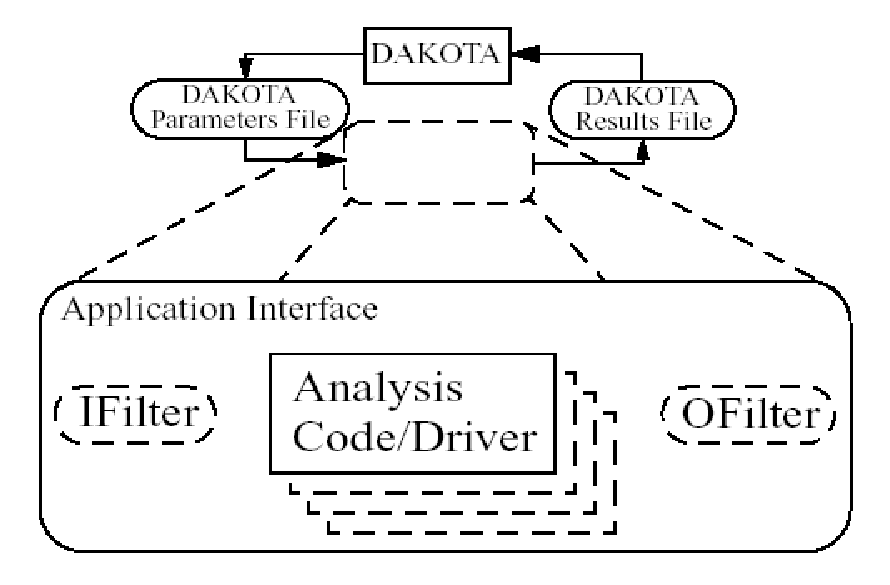
\includegraphics[scale=0.8]{images/dakota_components}
  \caption{Components of the simulation interface}
  \label{interfaces:bbinterfacecomp}
\end{figure}

When spawning function evaluations using system calls or forks, DAKOTA
must communicate parameter and response data with the analysis drivers
and filters through use of the file system. This is accomplished by
passing the names of the parameters and results files on the command
line when executing an analysis driver or filter. The input filter or
analysis driver read data from the parameters file and the output
filter or analysis driver write the appropriate data to the responses
file. While not essential when the file names are fixed, the file
names must be retrieved from the command line when DAKOTA is changing
the file names from one function evaluation to the next (i.e., using
temporary files or root names tagged with numerical identifiers).
In the case of a UNIX C-shell script, the two command line arguments
are retrieved using \texttt{\$argv[1]} and \texttt{\$argv[2]}
(see~\cite{And86}).  Similarly, Bourne shell scripts retrieve the two
command line arguments using \texttt{\$1} and \texttt{\$2}, and Perl
scripts retrieve the two command line arguments using
\texttt{@ARGV[0]} and \texttt{@ARGV[1]}.  In the case of a C or C++
program, command line arguments are retrieved using \texttt{argc}
(argument count) and \texttt{argv} (argument vector)~\cite{Ker88}, and
for Fortran 77, the \texttt{iargc} function returns the argument count
and the \texttt{getarg} subroutine returns command line arguments.

\subsection{Single analysis driver without filters}\label{interfaces:components:single1}

If a single \texttt{analysis\_driver} is selected in the interface
specification and filters are not needed (as indicated by omission of
the \texttt{input\_filter} and \texttt{output\_filter}
specifications), then only one process will appear in the execution
syntax of the simulation interface. An example of this syntax in the
system call case is:
\begin{small}
\begin{verbatim}
    driver params.in results.out
\end{verbatim}
\end{small}

where ``\texttt{driver}'' is the user-specified analysis driver and
``\texttt{params.in}'' and ``\texttt{results.out}'' are the names of the
parameters and results files, respectively, passed on the command
line. In this case, the user need not retrieve the command line
arguments since the same file names will be used each time.

For the same mapping, the fork simulation interface echoes the
following syntax:
\begin{small}
\begin{verbatim}
    blocking fork: driver params.in results.out
\end{verbatim}
\end{small}

for which only a single blocking fork is needed to perform the
evaluation.

Executing the same mapping with the direct simulation interface
results in an echo of the following syntax:
\begin{small}
\begin{verbatim}
    Direct function: invoking driver
\end{verbatim}
\end{small}

where this analysis driver must be linked as a function within
DAKOTA's direct interface (see Section~\ref{advint:direct}). Note that
no parameter or response files are involved, since such values
are passed directly through the function argument lists.

Both the system call and fork interfaces support asynchronous
operations. The asynchronous system call execution syntax involves
executing the system call in the background:
\begin{small}
\begin{verbatim}
    driver params.in.1 results.out.1 &
\end{verbatim}
\end{small}

and the asynchronous fork execution syntax involves use of a
nonblocking fork:
\begin{small}
\begin{verbatim}
    nonblocking fork: driver params.in.1 results.out.1
\end{verbatim}
\end{small}

where file tagging (see Section~\ref{interfaces:file:tagging1}) has
been user-specified in both cases to prevent conflicts between
concurrent analysis drivers. In these cases, the user must retrieve
the command line arguments since the file names change on each
evaluation.  Execution of the direct interface must currently be
performed synchronously since multithreading is not yet supported
(see Section~\ref{parallel:SLP:local:direct}).

\subsection{Single analysis driver with filters}\label{interfaces:components:single2}

When filters are used, the syntax of the system call that DAKOTA
performs is:
\begin{small}
\begin{verbatim}
    ifilter params.in results.out; driver params.in results.out;
         ofilter params.in results.out
\end{verbatim}
\end{small}

in which the input filter (``\texttt{ifilter}''), analysis driver
(``\texttt{driver}''), and output filter (``\texttt{ofilter}'')
processes are combined into a single system call through the use of
semi-colons (see~\cite{And86}). All three portions are
passed the names of the parameters and results files on the command
line.

For the same mapping, the fork simulation interface echoes the
following syntax:
\begin{small}
\begin{verbatim}
    blocking fork: ifilter params.in results.out;
         driver params.in results.out; ofilter params.in results.out
\end{verbatim}
\end{small}

where a series of three blocking forks is used to perform the
evaluation.

Executing the same mapping with the direct simulation interface
results in an echo of the following syntax:
\begin{small}
\begin{verbatim}
    Direct function: invoking { ifilter driver ofilter }
\end{verbatim}
\end{small}

where each of the three components must be linked as a function within
DAKOTA's direct interface. Since asynchronous operations are not yet
supported, execution simply involves invocation of each of the three
linked functions in succession. Again, no files are involved since
parameter and response data are passed directly through the function
argument lists.

Asynchronous executions would appear as follows for the system call
interface:
\begin{small}
\begin{verbatim}
    (ifilter params.in.1 results.out.1; driver params.in.1 results.out.1;
         ofilter params.in.1 results.out.1) &
\end{verbatim}
\end{small}

and, for the fork interface, as:
\begin{small}
\begin{verbatim}
    nonblocking fork: ifilter params.in.1 results.out.1;
         driver params.in.1 results.out.1; ofilter params.in.1 results.out.1
\end{verbatim}
\end{small}

where file tagging of evaluations has again been user-specified in
both cases. For the system call simulation interface, use of
parentheses and semi-colons to bind the three processes into a single
system call simplifies asynchronous process management compared to an
approach using separate system calls. The fork simulation interface,
on the other hand, does not rely on parentheses and accomplishes
asynchronous operations by first forking an intermediate process. This
intermediate process is then reforked for the execution of the input
filter, analysis driver, and output filter. The intermediate process
can be blocking or nonblocking (nonblocking in this case), and the
second level of forks can be blocking or nonblocking (blocking in this
case). The fact that forks can be reforked multiple times using either
blocking or nonblocking approaches provides the enhanced flexibility
to support a variety of local parallelism approaches (see
Chapter~\ref{parallel}).

\subsection{Multiple analysis drivers without filters}\label{interfaces:components:multiple1}

If a list of \texttt{analysis\_drivers} is specified and filters are
not needed (i.e., neither \texttt{input\_filter} nor
\texttt{output\_filter} appears), then the system call syntax
would appear as:
\begin{small}
\begin{verbatim}
    driver1 params.in results.out.1; driver2 params.in results.out.2;
         driver3 params.in results.out.3
\end{verbatim}
\end{small}

where ``\texttt{driver1}'', ``\texttt{driver2}'', and
``\texttt{driver3}'' are the user-specified analysis drivers and
``\texttt{params.in}'' and ``\texttt{results.out}'' are the
user-selected names of the parameters and results files. Note that the
results files for the different analysis drivers have been
automatically tagged to prevent overwriting. This automatic tagging of
\emph{analyses} (see Section~\ref{interfaces:file:tagging2}) is a
separate operation from user-selected tagging of \emph{evaluations}
(see Section~\ref{interfaces:file:tagging1}).

For the same mapping, the fork simulation interface echoes the
following syntax:
\begin{small}
\begin{verbatim}
    blocking fork: driver1 params.in results.out.1;
         driver2 params.in results.out.2; driver3 params.in results.out.3
\end{verbatim}
\end{small}

for which a series of three blocking forks is needed (no reforking of
an intermediate process is required).

Executing the same mapping with the direct simulation interface
results in an echo of the following syntax:
\begin{small}
\begin{verbatim}
    Direct function: invoking { driver1 driver2 driver3 }
\end{verbatim}
\end{small}

where, again, each of these components must be linked within DAKOTA's
direct interface and no files are involved for parameter and response
data transfer.

Both the system call and fork interfaces support asynchronous function
evaluations. The asynchronous system call execution syntax would be
reported as
\begin{small}
\begin{verbatim}
    (driver1 params.in.1 results.out.1.1; driver2 params.in.1 results.out.1.2;
         driver3 params.in.1 results.out.1.3) &
\end{verbatim}
\end{small}

and the nonblocking fork execution syntax would be reported as
\begin{small}
\begin{verbatim}
    nonblocking fork: driver1 params.in.1 results.out.1.1;
         driver2 params.in.1 results.out.1.2; driver3 params.in.1 results.out.1.3
\end{verbatim}
\end{small}

where, in both cases, file tagging of evaluations has been
user-specified to prevent conflicts between concurrent analysis
drivers and file tagging of the results files for multiple analyses is
automatically used. In the fork interface case, an intermediate
process is forked to allow a non-blocking function evaluation, and
this intermediate process is then reforked for the execution of each
of the analysis drivers.

\subsection{Multiple analysis drivers with filters}\label{interfaces:components:multiple2}

Finally, when combining filters with multiple
\texttt{analysis\_drivers}, the syntax of the system call that DAKOTA
performs is:
\begin{small}
\begin{verbatim}
    ifilter params.in.1 results.out.1;
         driver1 params.in.1 results.out.1.1;
         driver2 params.in.1 results.out.1.2;
         driver3 params.in.1 results.out.1.3;
         ofilter params.in.1 results.out.1
\end{verbatim}
\end{small}

in which all processes have again been combined into a single system
call through the use of semi-colons and parentheses. Note that the
secondary file tagging for the results files is only used for the
analysis drivers and not for the filters. This is consistent with the
filters' defined purpose of managing the non-repeated portions of
analysis pre- and post-processing (e.g., overlay of response results
from individual analyses; see Section~\ref{interfaces:file:tagging2}
for additional information).

For the same mapping, the fork simulation interface echoes the
following syntax:
\begin{small}
\begin{verbatim}
    blocking fork: ifilter params.in.1 results.out.1;
         driver1 params.in.1 results.out.1.1;
         driver2 params.in.1 results.out.1.2;
         driver3 params.in.1 results.out.1.3;
         ofilter params.in.1 results.out.1
\end{verbatim}
\end{small}

for which a series of five blocking forks is used (no reforking of an
intermediate process is required).

Executing the same mapping with the direct simulation interface
results in an echo of the following syntax:
\begin{small}
\begin{verbatim}
    Direct function: invoking { ifilter driver1 driver2 driver3 ofilter }
\end{verbatim}
\end{small}

where each of these components must be linked as a function within
DAKOTA's direct interface. Since asynchronous operations are not
supported, execution simply involves invocation of each of the five
linked functions in succession. Again, no files are involved for
parameter and response data transfer since this data is passed
directly through the function argument lists.

Asynchronous executions would appear as follows for the system call
interface:
\begin{small}
\begin{verbatim}
    (ifilter params.in.1 results.out.1;
         driver1 params.in.1 results.out.1.1;
         driver2 params.in.1 results.out.1.2;
         driver3 params.in.1 results.out.1.3;
         ofilter params.in.1 results.out.1) &
\end{verbatim}
\end{small}

and for the fork interface:
\begin{small}
\begin{verbatim}
    nonblocking fork: ifilter params.in.1 results.out.1;
         driver1 params.in.1 results.out.1.1;
         driver2 params.in.1 results.out.1.2;
         driver3 params.in.1 results.out.1.3;
         ofilter params.in.1 results.out.1
\end{verbatim}
\end{small}

where, again, user-selected file tagging of evaluations is combined
with automatic file tagging of analyses. In the fork interface case,
an intermediate process is forked to allow a non-blocking function
evaluation, and this intermediate process is then reforked for the
execution of the input filter, each of the analysis drivers, and the
output filter.

\section{Simulation File Management}\label{interfaces:file}

This section describes some management features used for files that
transfer data between DAKOTA and simulation codes
(i.e., when the system call or fork interfaces are used). These
features can generate unique filenames when
DAKOTA executes programs in parallel and can help one debug
the interface between DAKOTA and a simulation code.

\subsection{File Saving}\label{interfaces:file:saving}

{\bf Before driver execution:} In DAKOTA 5.0 and newer, an existing
results file will be removed immediately prior to executing the
analysis driver.  This new behavior addresses a common user problem
resulting from starting DAKOTA with stale results files in the run
directory.  To override this default behavior and preserve any
existing results files, specify \texttt{allow\_existing\_results}.

{\bf After driver execution:} The \texttt{file\_save} option in the
interface specification allows the user to control whether parameters
and results files are retained or removed from the working directory
after the analysis completes. DAKOTA's default behavior is to remove
files once their use is complete to reduce clutter. If the method
output setting is verbose, a file remove notification will follow the
function evaluation echo, e.g.,
\begin{small}
\begin{verbatim}
    driver /usr/tmp/aaaa20305 /usr/tmp/baaa20305
    Removing /usr/tmp/aaaa20305 and /usr/tmp/baaa20305
\end{verbatim}
\end{small}

However, if \texttt{file\_save} appears in the interface
specification, these files will not be removed. This latter behavior
is often useful for debugging communication between DAKOTA and
simulator programs. An example of a \texttt{file\_save} specification
is shown in the file tagging example below.

\subsection{File Tagging for Evaluations}\label{interfaces:file:tagging1}

When a user provides \texttt{parameters\_file} and
\texttt{results\_file} specifications, the \texttt{file\_tag} option
in the interface specification causes DAKOTA to make the names of
these files unique by appending the function
evaluation number to the root file names. Default behavior is to not
tag these files, which has the advantage of allowing the user to
ignore command line argument passing and always read to and write from
the same file names. However, it has the disadvantage that files may
be overwritten from one function evaluation to the next. When
\texttt{file\_tag} appears in the interface specification, the file names
are made unique by the appended evaluation number. This uniqueness
requires the user's interface to get the names of
these files from the command line. The file tagging feature is most
often used when concurrent simulations are running in a common disk
space, since it can prevent conflicts between the simulations. An
example specification of \texttt{file\_tag} and \texttt{file\_save} is
shown below:
\begin{small}
\begin{verbatim}
    interface,
            system
              analysis_driver = 'text_book'
              parameters_file = 'text_book.in'
              results_file    = 'text_book.out'
              file_tag file_save
\end{verbatim}
\end{small}

\emph{Special case:} When a user specifies names for the parameters
and results files and \texttt{file\_save} is used without
\texttt{file\_tag}, untagged files are used in the function evaluation
but are then moved to tagged files after the function evaluation is
complete, to prevent overwriting files for which a
\texttt{file\_save} request has been given. If the output control is
set to verbose, then a notification similar to the following will
follow the function evaluation echo:
\begin{small}
\begin{verbatim}
    driver params.in results.out
    Files with non-unique names will be tagged to enable file_save:
    Moving params.in to params.in.1
    Moving results.out to results.out.1
\end{verbatim}
\end{small}

\subsection{Temporary Files}\label{interfaces:file:temporary}

If \texttt{parameters\_file} and \texttt{results\_file} are not
specified by the user, temporary files having generated names are used.
For example, a system call to
a single analysis driver might appear as:
\begin{small}
\begin{verbatim}
    driver /usr/tmp/aaaa20305 /usr/tmp/baaa20305
\end{verbatim}
\end{small}

and a system call to an analysis driver with filter programs might appear as:
\begin{small}
\begin{verbatim}
    ifilter /usr/tmp/aaaa22490 usr/tmp/baaa22490;
         driver /usr/tmp/aaaa22490 usr/tmp/baaa22490;
         ofilter /usr/tmp/aaaa22490 /usr/tmp/baaa22490
\end{verbatim}
\end{small}

These files have unique names created by the \texttt{tmpnam}
utility from the C standard library~\cite{Ker88}. This uniqueness requires
the user's interface to get the names of
these files from the command line. File tagging with evaluation number
is unnecessary with temporary files (since they are already
unique); thus, \texttt{file\_tag} requests will be ignored. A
\texttt{file\_save} request will be honored, but it should be used
with care since the temporary file directory could easily become
cluttered without the user noticing.

\subsection{File Tagging for Analysis Drivers}\label{interfaces:file:tagging2}

When multiple analysis drivers are involved in performing a function
evaluation with either the system call or fork simulation interface,
a secondary file tagging is \emph{automatically} used to
distinguish the results files used for the individual analyses. This
applies to both the case of user-specified names for the parameters
and results files and the default temporary file case. Examples
for the former case were shown previously in
Section~\ref{interfaces:components:multiple1} and
Section~\ref{interfaces:components:multiple2}.  The following examples
demonstrate the latter temporary file case. Even though Unix
temporary files have unique names for a particular function
evaluation, tagging is still needed to manage the individual
contributions of the different analysis drivers to the response
results, since the same root results filename is used for each
component. For the system call interface, the syntax would be similar
to the following:
\begin{small}
\begin{verbatim}
    ifilter /var/tmp/aaawkaOKZ /var/tmp/baaxkaOKZ;
         driver1 /var/tmp/aaawkaOKZ /var/tmp/baaxkaOKZ.1;
         driver2 /var/tmp/aaawkaOKZ /var/tmp/baaxkaOKZ.2;
         driver3 /var/tmp/aaawkaOKZ /var/tmp/baaxkaOKZ.3;
         ofilter /var/tmp/aaawkaOKZ /var/tmp/baaxkaOKZ
\end{verbatim}
\end{small}

and, for the fork interface, similar to:
\begin{small}
\begin{verbatim}
    blocking fork:
         ifilter /var/tmp/aaawkaOKZ /var/tmp/baaxkaOKZ;
         driver1 /var/tmp/aaawkaOKZ /var/tmp/baaxkaOKZ.1;
         driver2 /var/tmp/aaawkaOKZ /var/tmp/baaxkaOKZ.2;
         driver3 /var/tmp/aaawkaOKZ /var/tmp/baaxkaOKZ.3;
         ofilter /var/tmp/aaawkaOKZ /var/tmp/baaxkaOKZ
\end{verbatim}
\end{small}

Tagging of results files with an analysis identifier is needed
since each analysis driver must contribute a
user-defined subset of the total response results for the evaluation.
If an output filter is not supplied, DAKOTA will combine these
portions through a simple overlaying of the individual contributions
(i.e., summing the results in \texttt{/var/tmp/baaxkaOKZ.1},
\texttt{/var/tmp/baaxkaOKZ.2}, and \texttt{/var/tmp/baaxkaOKZ.3}). If
this simple approach is inadequate, then an output filter should be
supplied to perform the combination. This is the reason why the
results file for the output filter does not use analysis tagging; it
is responsible for the results combination (i.e., combining
\texttt{/var/tmp/baaxkaOKZ.1}, \texttt{/var/tmp/baaxkaOKZ.2}, and
\texttt{/var/tmp/baaxkaOKZ.3} into \texttt{/var/tmp/baaxkaOKZ}). In
this case, DAKOTA will read only the results file from the output
filter (i.e., \texttt{/var/tmp/baaxkaOKZ}) and interpret it as the
total response set for the evaluation.

Parameters files are not currently tagged with an analysis identifier.
This reflects the fact that DAKOTA does not attempt to subdivide the
requests in the active set vector for different analysis portions.
Rather, the total active set vector is passed to each analysis driver
and the appropriate subdivision of work \emph{must be defined by the
  user}. This allows the division of labor to be very flexible. In
some cases, this division might occur across response functions, with
different analysis drivers managing the data requests for different
response functions. And in other cases, the subdivision might occur
within response functions, with different analysis drivers
contributing portions to each of the response functions. The only
restriction is that each of the analysis drivers must follow the
response format dictated by the total active set vector. For response
data for which an analysis driver has no contribution, 0's must be
used as placeholders.

\subsection{Work Directories}\label{interfaces:workdir}

Sometimes it is convenient for simulators and filters to run in a directory
different from the one where DAKOTA is invoked.  A simulator script
used as an \texttt{analysis\_driver}
can of course change to a different directory if desired (while still arranging
to write a results file in the original directory), but
DAKOTA 5.0 has new facilities that may simplify the creation of
simulator scripts.
% for use with the fork or system interface.
If an interface specification includes the keyword
\begin{small}
\begin{verbatim}
       work_directory
\end{verbatim}
\end{small}
then DAKOTA will arrange for the simulator and any filters to
wake up in the work directory, with \$PATH adjusted (if necessary)
so programs that could be invoked without a relative
path to them (i.e., by a name not involving any slashes) from
DAKOTA's directory can also be invoked from the simulator's (and filter's)
directory.  On occasion, it is convenient for the simulator to have
various files, e.g., data files, available in the directory where it
runs.  If, say, \texttt{my/special/directory} is such a directory
(as seen from DAKOTA's directory), the interface specification
\begin{small}
\begin{verbatim}
       work_directory named 'my/special/directory'
\end{verbatim}
\end{small}
would cause DAKOTA to start the simulator and any filters in that directory.
If the directory did not already exist, DAKOTA would create it
and would remove it after the simulator (or output filter, if specifed)
finished, unless instructed not to do so
by the appearance of \texttt{directory\_save} or its synonym \texttt{dir\_save}
in the interface specification.  If \texttt{named '$...$'} does not
appear, then \texttt{directory\_save} cannot appear either, and
DAKOTA creates a temporary directory (using the \texttt{tmpnam}
function to determine its name) for use by the simulator and any filters.
If you specify \texttt{directory\_tag} (or \texttt{dir\_tag}),
DAKOTA causes each invocation of the simulator and any filters to start in a
a subdirectory of the work directory with a name composed
of the work directory's name followed by a period and the
invocation number (1, 2, $...$); this might be useful in debugging.

Sometimes it can be helpful for the simulator and filters to start in a
new directory populated with some files.  Adding
\begin{small}
\begin{verbatim}
       template_directory 'my/template'
\end{verbatim}
\end{small}
to the work directory specification would cause the
contents of directory \texttt{my/template} to be linked recursively
into the work directory.  Linking makes sense if files are large,
but when practical, it is far more reliable to have
copies of the files; adding \texttt{copy} to the specification
would cause the contents of the template directory to be copied
recursively to the work directory.  The linking or copying does
not replace existing files unless \texttt{replace} also appears
in the specification.  Instead of \texttt{template\_directory} $...$,
you can specify \texttt{template\_files}, followed by one or more
quoted strings, as in
\begin{small}
\begin{verbatim}
       template_files 'zip' 'zap' 'foo/zot'
\end{verbatim}
\end{small}
which would cause \texttt{zip}, \texttt{zap}, and \texttt{foo/zot} to
be linked (or, with \texttt{copy}, copied) recursively to the work
directory.

Here is a summary of possibilities for a work directory specification,
with {\tt\verb=[=$...$\verb=]=} denoting that $...$ is optional:
\begin{small}
\begin{verbatim}
        work_directory [ named '...' ]
          [ directory_tag ]     # or dir_tag
          [ directory_save ]    # or dir_save
          [ template_directory '...' # or template_files '...' '...' ...
             [ copy ]
             [ replace ]
             ]
\end{verbatim}
\end{small}

\section{Parameter to Response Mappings}\label{interfaces:mappings}

In this section, interface mapping examples are presented through the
discussion of several parameters files and their corresponding results
files. A typical input file for 2 variables ($n=2$) and 3 functions
($m=3$) using the standard parameters file format (see
Section~\ref{variables:parameters:standard}) is as follows:
\begin{small}
\begin{verbatim}
                        2 variables
    1.500000000000000e+00 cdv_1
    1.500000000000000e+00 cdv_2
                        3 functions
                        1 ASV_1
                        1 ASV_2
                        1 ASV_3
                        2 derivative_variables
                        1 DVV_1
                        2 DVV_2
                        0 analysis_components
\end{verbatim}
\end{small}
where numerical values are associated with their tags within
``\texttt{value tag}'' constructs. The number of design variables
($n$) and the string ``\texttt{variables}'' are followed by the values
of the design variables and their tags, the number of functions ($m$)
and the string ``\texttt{functions}'', the active set vector (ASV) and
its tags, the number of derivative variables and the string
``\texttt{derivative\_variables}'', the derivative variables vector
(DVV) and its tags, the number of analysis components and the string
``\texttt{analysis\_components}'', and the analysis components array
and its tags.  The descriptive tags for the variables are always
present and they are either the descriptors in the user's variables
specification, if given there, or are default descriptors.  The length
of the active set vector is equal to the number
of functions ($m$). In the case of an optimization data set with an
objective function and two nonlinear constraints (three response
functions total), the first ASV value is associated with the objective
function and the remaining two are associated with the constraints (in
whatever consistent constraint order has been defined by the user).
The DVV defines a subset of the variables used for computing
derivatives.  Its identifiers are 1-based and correspond to the full
set of variables listed in the first array.  Finally, the analysis
components pass additional strings from the user's
\texttt{analysis\_components} specification in a DAKOTA input file
through to the simulator.  They allow the development of simulation
drivers that are more flexible, by allowing them to be passed
additional specifics at run time, e.g., the names of model files such
as a particular mesh to use.

For the APREPRO format option (see
Section~\ref{variables:parameters:aprepro}), the same set of data
appears as follows:
\begin{small}
\begin{verbatim}
    { DAKOTA_VARS     =                      2 }
    { cdv_1           =  1.500000000000000e+00 }
    { cdv_2           =  1.500000000000000e+00 }
    { DAKOTA_FNS      =                      3 }
    { ASV_1           =                      1 }
    { ASV_2           =                      1 }
    { ASV_3           =                      1 }
    { DAKOTA_DER_VARS =                      2 }
    { DVV_1           =                      1 }
    { DVV_2           =                      2 }
    { DAKOTA_AN_COMPS =                      0 }
\end{verbatim}
\end{small}

where the numerical values are associated with their tags within
``\texttt{\{ tag = value \}}'' constructs.

The user-supplied simulation interface, comprised of a simulator
program or driver and (optionally) filter programs, is responsible for
reading the parameters file and creating a results file that contains
the response data requested in the ASV. This response data is written
in the format described in Section~\ref{responses:results}. Since the
ASV contains all ones in this case, the response file corresponding to
the above input file would contain values for the three functions:
\begin{small}
\begin{verbatim}
    1.250000000000000e-01 f
    1.500000000000000e+00 c1
    1.500000000000000e+00 c2
\end{verbatim}
\end{small}

Since function tags are optional, the following would be equally
acceptable:
\begin{small}
\begin{verbatim}
    1.250000000000000e-01
    1.500000000000000e+00
    1.500000000000000e+00
\end{verbatim}
\end{small}

For the same parameters with different ASV components,
\begin{small}
\begin{verbatim}
                        2 variables
    1.500000000000000e+00 cdv_1
    1.500000000000000e+00 cdv_2
                        3 functions
                        3 ASV_1
                        3 ASV_2
                        3 ASV_3
                        2 derivative_variables
                        1 DVV_1
                        2 DVV_2
                        0 analysis_components
\end{verbatim}
\end{small}

the following response data is required:
\begin{small}
\begin{verbatim}
    1.250000000000000e-01 f
    1.500000000000000e+00 c1
    1.500000000000000e+00 c2
    [ 5.000000000000000e-01 5.000000000000000e-01 ]
    [ 3.000000000000000e+00 -5.000000000000000e-01 ]
    [ -5.000000000000000e-01 3.000000000000000e+00 ]
\end{verbatim}
\end{small}
Here, we need not only the function values, but also each of their
gradients. The derivatives are computed with respect to \texttt{cdv\_1}
and \texttt{cdv\_2} as indicated by the DVV values. Another modification
to the ASV components yields the following parameters file:
\begin{small}
\begin{verbatim}
                        2 variables
    1.500000000000000e+00 cdv_1
    1.500000000000000e+00 cdv_2
                        3 functions
                        2 ASV_1
                        0 ASV_2
                        2 ASV_3
                        2 derivative_variables
                        1 DVV_1
                        2 DVV_2
                        0 analysis_components
\end{verbatim}
\end{small}

for which the following results file is needed:
\begin{small}
\begin{verbatim}
    [ 5.000000000000000e-01 5.000000000000000e-01 ]
    [ -5.000000000000000e-01 3.000000000000000e+00 ]
\end{verbatim}
\end{small}
Here, we need gradients for functions \texttt{f} and \texttt{c2}, but
not for \texttt{c1}, presumably since this constraint is inactive.

A full Newton optimizer might make the following request:
\begin{small}
\begin{verbatim}
                        2 variables
    1.500000000000000e+00 cdv_1
    1.500000000000000e+00 cdv_2
                        1 functions
                        7 ASV_1
                        2 derivative_variables
                        1 DVV_1
                        2 DVV_2
                        0 analysis_components
\end{verbatim}
\end{small}

for which the following results file,
\begin{small}
\begin{verbatim}
    1.250000000000000e-01 f
    [ 5.000000000000000e-01 5.000000000000000e-01 ]
    [[ 3.000000000000000e+00 0.000000000000000e+00
       0.000000000000000e+00 3.000000000000000e+00 ]]
\end{verbatim}
\end{small}
containing the objective function, its gradient vector, and its
Hessian matrix, is needed.  Again, the derivatives (gradient vector
and Hessian matrix) are computed with respect to \texttt{cdv\_1} and
\texttt{cdv\_2} as indicated by the DVV values.

Lastly, a more advanced example could have multiple types of variables
present; in this example, 2 continuous design and 3 discrete design
range, 2 normal uncertain, and 3 continuous state and 2 discrete state
range variables.  When a mixture of variable types is present, the
content of the DVV (and therefore the required length of gradient
vectors and Hessian matrices) depends upon the type of study being
performed (see Section~\ref{responses:active}).  For a reliability
analysis problem, the uncertain variables are the active continuous
variables and the following parameters file would be typical:
\begin{small}
\begin{verbatim}
                       12 variables
    1.500000000000000e+00 cdv_1
    1.500000000000000e+00 cdv_2
                        2 ddriv_1
                        2 ddriv_2
                        2 ddriv_3
    5.000000000000000e+00 nuv_1
    5.000000000000000e+00 nuv_2
    3.500000000000000e+00 csv_1
    3.500000000000000e+00 csv_2
    3.500000000000000e+00 csv_3
                        4 dsriv_1
                        4 dsriv_2
                        3 functions
                        3 ASV_1
                        3 ASV_2
                        3 ASV_3
                        2 derivative_variables
                        6 DVV_1
                        7 DVV_2
                        2 analysis_components
                mesh1.exo AC_1
                  db1.xml AC_2
\end{verbatim}
\end{small}

Gradients are requested with respect to variable entries 6 and 7,
which correspond to normal uncertain variables \texttt{nuv\_1} and
\texttt{nuv\_2}.  The following response data would be appropriate:
\begin{small}
\begin{verbatim}
    7.943125000000000e+02 f
    1.500000000000000e+00 c1
    1.500000000000000e+00 c2
    [ 2.560000000000000e+02 2.560000000000000e+02 ]
    [ 0.000000000000000e+00 0.000000000000000e+00 ]
    [ 0.000000000000000e+00 0.000000000000000e+00 ]
\end{verbatim}
\end{small}

In a parameter study, however, no distinction is drawn between
different types of continuous variables, and derivatives would be
needed with respect to all continuous variables ($n_{dvv}=7$ for the
continuous design variables \texttt{cdv\_1} and \texttt{cdv\_2}, the
normal uncertain variables \texttt{nuv\_1} and \texttt{nuv\_2}, and
the continuous state variables \texttt{csv\_1}, \texttt{csv\_2} and
\texttt{csv\_3}).  The parameters file would appear as
\begin{small}
\begin{verbatim}
                       12 variables
    1.500000000000000e+00 cdv_1
    1.500000000000000e+00 cdv_2
                        2 ddriv_1
                        2 ddriv_2
                        2 ddriv_3
    5.000000000000000e+00 nuv_1
    5.000000000000000e+00 nuv_2
    3.500000000000000e+00 csv_1
    3.500000000000000e+00 csv_2
    3.500000000000000e+00 csv_3
                        4 dsriv_1
                        4 dsriv_2
                        3 functions
                        3 ASV_1
                        3 ASV_2
                        3 ASV_3
                        7 derivative_variables
                        1 DVV_1
                        2 DVV_2
                        6 DVV_3
                        7 DVV_4
                        8 DVV_5
                        9 DVV_6
                       10 DVV_7
                        2 analysis_components
                mesh1.exo AC_1
                  db1.xml AC_2
\end{verbatim}
\end{small}

and the corresponding results would appear as
\begin{small}
\begin{verbatim}
    7.943125000000000e+02 f
    1.500000000000000e+00 c1
    1.500000000000000e+00 c2
    [  5.000000000000000e-01  5.000000000000000e-01  2.560000000000000e+02
       2.560000000000000e+02  6.250000000000000e+01  6.250000000000000e+01
       6.250000000000000e+01 ]
    [  3.000000000000000e+00 -5.000000000000000e-01  0.000000000000000e+00
       0.000000000000000e+00  0.000000000000000e+00  0.000000000000000e+00
       0.000000000000000e+00 ]
    [ -5.000000000000000e-01  3.000000000000000e+00  0.000000000000000e+00
       0.000000000000000e+00  0.000000000000000e+00  0.000000000000000e+00
       0.000000000000000e+00 ]
\end{verbatim}
\end{small}

\chapter{Responses}\label{responses}

\section{Overview}\label{responses:overview}

The \texttt{responses} specification in a Dakota input file controls
the types of data that can be returned from an interface during
Dakota's execution. The specification includes the number and type of
response functions (objective functions, nonlinear constraints, calibration 
terms, etc.) as well as availability of first and second
derivatives (gradient vectors and Hessian matrices) for these response
functions.

This chapter will present a brief overview of the response data sets
and their uses, as well as cover some user issues relating to file
formats and derivative vector and matrix sizing. For a detailed
description of responses section syntax and example specifications,
refer to the Responses Commands chapter in the Dakota Reference
Manual~\cite{RefMan}.

\subsection{Response function types}\label{responses:overview:types}

The types of response functions listed in the responses
specification should be consistent with the
iterative technique called for in the method specification:

\begin{itemize}

\item an optimization data set comprised of
  \texttt{num\_objective\_functions},\\
  \texttt{num\_nonlinear\_inequality\_constraints}, and
  \texttt{num\_nonlinear\_equality\_constraints}.  This data set is
  appropriate for use with optimization methods (e.g., the methods in
  Section~\ref{capabilities:optimization1}).
  
\item a calibration data set comprised of 
  \texttt{calibration\_terms},\\
  \texttt{num\_nonlinear\_inequality\_constraints}, and
  \texttt{num\_nonlinear\_equality\_constraints}.  This data set is
  appropriate for use with nonlinear least squares algorithms
  (e.g., the methods in Section~\ref{capabilities:nonlinear}).
  
\item a generic data set comprised of \texttt{num\_response\_functions}.  
  This data set is appropriate for use with uncertainty quantification
  methods (e.g., the methods in Section~\ref{capabilities:uncertainty}).
  
\end{itemize}

Certain general-purpose iterative techniques, such as parameter
studies and design of experiments methods, can be used with any of
these data sets.

\subsection{Gradient availability}\label{responses:overview:gradient}

Gradient availability for these response functions may be described by:

\begin{itemize}

\item \texttt{no\_gradients}: gradients will not be used.

\item \texttt{numerical\_gradients}: gradients are needed and will
  be approximated by finite differences.

\item \texttt{analytic\_gradients}: gradients are needed and will be supplied
  by the simulation code (without any finite differencing by Dakota).

\item \texttt{mixed\_gradients}: the simulation will supply some gradient
  components and Dakota will approximate the others by finite
  differences.

\end{itemize}

The gradient specification also links back to the iterative method
used. Gradients commonly are needed when the iterative
study involves gradient-based optimization, reliability analysis for
uncertainty quantification, or local sensitivity analysis.

\subsection{Hessian availability}\label{responses:overview:hessian}

Hessian availability for the response functions is similar to the
gradient availability specifications, with the addition of support
for ``quasi-Hessians":

\begin{itemize}

\item \texttt{no\_hessians}: Hessians will not be used.

\item \texttt{numerical\_gradients}: Hessians are needed and will be
  approximated by finite differences.  These finite differences may be
  involve first-order differences of gradients (if analytic gradients
  are available for the response function of interest) or second-order 
  differences of function values (in all other cases).

\item \texttt{quasi\_hessians}: Hessians are needed and will be 
  approximated by secant updates (BFGS or SR1) from a series of 
  gradient evaluations.

\item \texttt{analytic\_hessians}: Hessians are needed and are
  available directly from the simulation code.

\item \texttt{mixed\_hessians}: Hessians are needed and will be 
  obtained from a mix of numerical, analytic, and ``quasi" sources.

\end{itemize}

The Hessian specification also links back to the iterative method in
use; Hessians commonly would be used in gradient-based
optimization by full Newton methods or in reliability analysis
with second-order limit state approximations or second-order
probability integrations.

\section{Dakota Results File Data Format}\label{responses:results}

Simulation interfaces using system calls and forks to create
separate simulation processes must communicate with the simulation
through the file system. This is done by reading and
writing files of parameters and results. Dakota uses its own format
for this data input/output. For the results file, only one format is
supported (versus the two parameter-file formats described in
Section~\ref{variables:parameters}). Ordering of response functions is
as listed in Section~\ref{responses:overview:types} (e.g., objective
functions or calibration terms are first, followed by nonlinear
inequality constraints, followed by nonlinear equality constraints).

After a simulation, Dakota expects to read a file
containing responses reflecting the current parameters and
corresponding to the function requests in the active
set vector. The response data must be in the format
shown in Figure \ref{responses:figure01}.

\begin{figure}
  \centering
  \begin{bigbox}
  \begin{alltt}
    <double> <fn_tag\(\sb{1}\)>
    <double> <fn_tag\(\sb{2}\)>
    ...
    <double> <fn_tag\(\sb{m}\)> \color{blue}
    [ <double> <double> .. <double> ]
    [ <double> <double> .. <double> ]
    ...
    [ <double> <double> .. <double> ] \color{red}
    [[ <double> <double> .. <double> ]]
    [[ <double> <double> .. <double> ]]
    ...
    [[ <double> <double> .. <double> ]]
  \end{alltt}
  \end{bigbox}
  \caption{Results file data format.}
  \label{responses:figure01}
\end{figure}

The first block of data (shown in black) conveys the requested function values
and is followed by a block of requested gradients
(shown in blue), followed by a block of requested Hessians (shown
in red). If the amount of data in the file does not match the function
request vector, Dakota will abort execution with an error message.

Function values have no bracket delimiters and \emph{optionally} one
character-string tag per function can be supplied.  These tags are not
used by
Dakota and are only included as an optional field for consistency with
the parameters file format and for backwards compatibility.  If
tags are used, they must be separated from
numeric function values by white space (one or more blanks, tabs, or newline
characters) and there must not
be any white space embedded within a character-string tag (e.g., use
``\texttt{variable1}'' or ``\texttt{variable\_1},'' but not
``\texttt{variable 1}'').

Gradient vectors are surrounded by single brackets
[\ldots$n_{dvv}$-vector of doubles\ldots]. Tags are not used and must
not be present. White space separating the brackets from the data is
optional.

Hessian matrices are surrounded by double brackets
[[\ldots$n_{dvv} \times n_{dvv}$ matrix of doubles\ldots]].  Hessian
components (numeric values for second partial derivatives) are
listed by rows and separated by white space; in particular, they
can be spread across multiple
lines for readability.  Tags are not used and must not be present.
White space after the initial double bracket and before the final one
is optional, but none can appear within the double brackets.

The format of the numeric fields may be floating point or scientific
notation. In the latter case, acceptable exponent characters are
``\texttt{E}'' or ``\texttt{e.}'' A common problem when dealing with
Fortran programs is that a C++ read of a numeric field using
``\texttt{D}'' or ``\texttt{d}'' as the exponent (i.e., a double
precision value from Fortran) may fail or be truncated. In this case,
the ``\texttt{D}'' exponent characters must be replaced either through
modifications to the Fortran source or compiler flags or through a
separate post-processing step (e.g., using the UNIX \texttt{sed}
utility).

\section{Active Variables for Derivatives}\label{responses:active}

An important question for proper management of both gradient and
Hessian data is: if several different types of variables are used,
\emph{for which variables are response function derivatives needed?}
That is, how is $n_{dvv}$ determined?  The short answer is that the
derivative variables vector (DVV) specifies the set of variables to be
used for computing derivatives, and $n_{dvv}$ is the length of this
vector.  The long answer is that, in most cases, the DVV is defined
directly from the set of active continuous variables for the iterative
method in use.

Since methods determine what subset, or view, of the variables is
active in the iteration, it is this same set of variables for which
derivatives are most commonly computed (see also
Section~\ref{variables:mixed}).  Derivatives are never needed with
respect to any discrete variables (since these derivatives do not in
general exist) and the active continuous variables depend on the type
of study being performed. For optimization and calibration problems,
the active continuous variables are the \emph{continuous design
  variables} ($n_{dvv}=n_{cdv}$), since they are the variables the
minimizer manipulates.  Similarly, for uncertainty quantification
methods that use gradient and/or Hessian information, the active
continuous variables are the \emph{continuous uncertain variables}
($n_{dvv}=n_{cauv}$ for aleatory methods, $n_{dvv}=n_{ceuv}$ for
epistemic methods, $n_{dvv}=n_{cauv}+n_{ceuv}$ for methods that handle
both), with the exception of \texttt{all\_variables} mode.  And
lastly, parameter study methods that are cataloging gradient and/or
Hessian information do not draw a distinction among continuous
variables; therefore, the active continuous variables are defined from
\emph{all continuous variables} that are specified
($n_{dvv}=n_{cdv}+n_{cauv}+n_{ceuv}+n_{csv}$).  Additional detail on
these variables views is provided in Table~\ref{responses:active_tab}.

\begin{table}
\centering
\caption{Variable views for different iterators.}
\label{responses:active_tab}\vspace{2mm}
\begin{tabular}{|c|c|c|}
\hline
\textbf{Method} & \textbf{Active view} & \textbf{Derivative variables} \\
\hline
branch and bound         & Merged Design   & $n_{cdv}+n_{ddiv}+n_{ddrv}$ \\
\hline
optimization,            & Mixed Design    & $n_{cdv}$ \\
nonlinear least squares  &                 &           \\
\hline
sampling (standard mode) & Mixed Uncertain & $n_{cauv}+n_{ceuv}$ \\
\hline
local reliability,       & Mixed Aleatory Uncertain & $n_{cauv}$ \\
global reliability (standard mode),  &              &            \\
stochastic expansion (standard mode) &              &            \\
\hline
interval estimation,     & Mixed Epistemic Uncertain & $n_{ceuv}$ \\
evidence                 &                           &            \\
\hline
parameter studies,       & Mixed All & $n_{cdv}+n_{cauv}+n_{ceuv}+n_{csv}$\\
design of experiments,   &           & \\
uncertainty quantification (all\_variables mode) & & \\
\hline
\end{tabular}
\end{table}

In a few cases, derivatives are needed with respect to the
\emph{inactive} continuous variables.  This occurs for nested
iteration where a top-level iterator sets derivative requirements
(with respect to its active continuous variables) on the final
solution of the lower-level iterator (for which the top-level active
variables are inactive).  For example, in an uncertainty analysis
within a nested design under uncertainty algorithm, derivatives of the
lower-level response functions may be needed with respect to the
design variables, which are active continuous variables at the top
level but are inactive within the uncertainty quantification.  These
instances are the reason for the creation and inclusion of the DVV
vector --- to clearly indicate the variables whose partial derivatives
are needed.

In all cases, if the DVV is honored, then the correct derivative
components are returned.  In simple cases, such as optimization and
calibration studies that only specify design variables and for
nondeterministic analyses that only specify uncertain variables,
derivative component subsets are not an issue and the exact content of
the DVV may be safely ignored.

\chapter{Inputs to Dakota}\label{input}

\section{Overview of Inputs}\label{input:overview}

Dakota supports a number of command-line arguments, as described in
Section~\ref{tutorial:installation:running}.  Among these are
specifications for the Dakota input file and, optionally, a restart
file.  The syntax of the Dakota input file is described in detail in
the Dakota Reference Manual~\cite{RefMan}, and the restart file is
described in Chapter~\ref{restart}.

A Dakota input file may be prepared manually with a text editor such
as Emacs, Vi, or WordPad, or it may be defined with the JAGUAR Dakota
graphical user interface.  The JAGUAR Dakota GUI is built on the
Java-based Eclipse Framework \cite{Eclipse} and presents the Dakota
input specification options in synchronized text-editing and graphical
views.  JAGUAR includes templates and wizards for helping create
Dakota studies and can invoke Dakota to run an analysis.  The Dakota
GUI for Linux, Windows, and Mac, is available for download from the
Dakota website \url{http://dakota.sandia.gov/}, along with licensing
information, separate GUI documentation, and installation tips.

\subsection{Tabular Data Formats}\label{input:tabularformat}

The Dakota input file and/or command line may identify additional
files for data import as described in Section~\ref{input:import}.
Some of these files are in tabular data format.

Dakota versions 5.1+ (October 2011) and newer use two formats for
tabular data file input and output.  Tabular data refer to numeric
data in text form related to, e.g., tabular graphics data, least
squares and Bayesian calibration data, samples/points files for
constructing surrogates, pre-run output, and post-run input.  Both
formats are written/read with C++ stream operators/conversions, so
most integer and floating point formats are acceptable for numeric
data.  The formats are:

\begin{itemize}
  \item {\bf Annotated Matrix} (default for all I/O; specified via
    {\tt annotated}): text file with one leading row of comments/column
    labels and one leading column of evaluation/row IDs surrounding
    num\_rows x num\_cols whitespace-separated numeric data, (newlines
    separating rows are not currently required, but may be in the
    future).  The numeric data in a row may correspond to variables,
    variables followed by responses, data point for calibration, etc.,
    depending on context.

   \item {\bf Free-form Matrix} (optional; previously default for
     samples files and least squares data; specified via {\tt
       freeform}): text file with no leading row and no leading
     column.  The num\_rows x num\_cols total numeric data entries may
     appear separated with any whitespace including arbitrary spaces,
     tabs, and newlines.  In this format, vectors may therefore appear
     as a single row or single column (or mixture; entries will
     populate the vector in order).
\end{itemize}

{\bf Attention:} Prior to October 2011, calibration and surrogate data
files were free-form format.  They now default to annotated format,
though {\tt freeform} remains an option.  For both formats, a warning
will be generated if a specific number of data are expected, but extra
is found and an error generated when there is insufficient data.  Some
TPLs like SCOLIB and JEGA manage their own file I/O and only support
the free-form option.

\section{Data Imports}\label{input:import}

The Dakota input file and/or command line may identify additional
files used to import data into Dakota.

\subsection{AMPL algebraic mappings: stub.nl, stub.row, and stub.col}

As described in Section~\ref{interfaces:algebraic}, an AMPL
specification of algebraic input-to-output relationships may be
imported into Dakota and used to define or augment the mappings of a
particular interface.

\subsection{Genetic algorithm population import}

Genetic algorithms (GAs) from the JEGA and SCOLIB packages support a
population import feature using the keywords
\texttt{initialization\_type flat\_file = \emph{STRING}}.  This is
useful for warm starting GAs from available data or previous runs.
Refer to the Method Specification chapter in the Dakota Reference
Manual~\cite{RefMan} for additional information on this specification.
The flat file must be in free-form format as described in
Section~\ref{input:tabularformat}.

\subsection{Calibration (least squares) data import}

Deterministic least squares and Bayesian Calibration methods allow
specification of experimental observations to difference with
responses in calculating a model misfit metric (such as a sum of
squared residuals).  The default file format is {\tt annotated}, but
the {\tt freeform} option is supported.  The data file should contain
one row per experiment.   The columns of the data file contain, in sequence
\begin{itemize}
\item {\bf configuration variables (optional):} state variable values
  indicating the configuration at which this experiment was conducted;
  length must agree with thee number of state variables active in the
  study.
\item {\bf experimental observations (required):} experimental data
  values to difference with model responses; length number of
  responses.
\item {\bf experimental standard deviations (optional):} measurement
  errors (standard deviations) associated with the data; length 1
  (same value for each model response) or num\_responses.
\end{itemize}
See~\ref{nls:examples} and the Dakota Reference Manual Responses
section for further details.

\subsection{PCE coefficient import}

Polynomial chaos expansion (PCE) methods compute coefficients for
response expansions which employ a basis of multivariate orthogonal
polynomials.  Normally, the \texttt{polynomial\_chaos} method
calculates these coefficients based either on a spectral projection or
a linear regression (see Section~\ref{uq:expansion}).  However,
Dakota also supports the option of importing a set of response PCE
coefficients based on the specification \\
\texttt{expansion\_import\_file = \emph{STRING}}.  This is useful for
evaluating moments analytically or computing probabilities numerically
from a known response expansion.  Refer to the Method Specification
chapter in the Dakota Reference Manual~\cite{RefMan} for additional
information on this specification.

\subsection{Surrogate construction from data files}

Global data fit surrogates may be constructed from a variety of data
sources.  One of these sources is an auxiliary data file, as specified
by the keywords \texttt{reuse\_samples points\_file = \emph{STRING}}.
The file may be in annotated (default) or free-form format with
columns corresponding to variables and responses.  Refer to the Model
Specification chapter in the Dakota Reference Manual~\cite{RefMan} for
additional information on this specification.

\subsection{Variables/responses import to post-run}

The post-run mode (supported only for sampling, parameter study, and
DACE methods) requires specification of a file containing parameter
and response data in annotated tabular format (see Section
~\ref{input:tabularformat}; free-form is not supported).  An
evaluation ID column is followed by columns for variables, then those
for responses, with an ignored header row of labels and then one row
per evaluation.  Typically this file would be generated by executing
\texttt{dakota -i dakota.in -pre\_run ::variables.dat} and then adding
columns of response data to variables.dat to make varsresponses.dat.
The file is specified at the command line with:
\begin{small}
\begin{verbatim}
    dakota -i dakota.in -post_run varsresponses.dat::
\end{verbatim}
\end{small}

%PCE coefficients

\chapter{Output from Dakota}\label{output}

\section{Overview of Output Formats}\label{output:overview}

Given an emphasis on complex numerical simulation codes that run on
massively parallel supercomputers, Dakota's output has been designed
to provide a succinct, text-based reporting of the progress of the
iterations and function evaluations performed by an algorithm. In
addition, Dakota provides a tabular output format that is useful for
data visualization with external tools and a basic graphical output
capability that is useful as a monitoring tool. The JAGUAR Dakota GUI
is an emerging capability that will provide more advanced
visualization facilities in time.

\section{Standard Output}\label{output:standard}

Dakota outputs basic information to ``standard out'' (i.e., the
screen) for each function evaluation, consisting of an evaluation
number, parameter values, execution syntax, the active set vector, and
the response data set. To describe the standard output of Dakota,
optimization of the ``container'' problem (see
Chapter~\ref{additional} for problem formulation) is used as an
example. The input file for this example is shown in
Figure~\ref{output:incont}. In this example, there is one equality
constraint, and Dakota's finite difference algorithm is used to
provide central difference numerical gradients to the NPSOL optimizer.
\begin{figure}
  \begin{small}
    \begin{bigbox}
      \verbatimtabinput[8]{container_opt_npsol.in}
    \end{bigbox}
  \end{small}
  \caption{Dakota input file for the ``container'' test problem --
see \texttt{Dakota/examples/users/container\_opt\_npsol.in} }
  \label{output:incont}
\end{figure}

\clearpage

A partial listing of the Dakota output for the container optimization
example follows:
\begin{small}
\begin{verbatim}
Running MPI executable in serial mode.
Dakota version 5.0 released 12/21/2009.
Subversion revision 5635M built Dec 18 2009 17:19:56.
Constructing Single Method Strategy...
Writing new restart file dakota.rst
methodName = npsol_sqp
gradientType = numerical
Numerical gradients using central differences
to be calculated by the dakota finite difference routine.
hessianType = none

>>>>> Running Single Method Strategy.

>>>>> Running npsol_sqp iterator.





                     NPSOL  ---  Version 5.0-2      Sept 1995
                     ========================================

------------------------------------------
Begin Dakota derivative estimation routine
------------------------------------------

>>>>> Initial map for analytic portion of response:

------------------------------
Begin Function Evaluation    1
------------------------------
Parameters for function evaluation 1:
                      4.5000000000e+00 H
                      4.5000000000e+00 D

container container.in.1 container.out.1

Active response data for function evaluation 1:
Active set vector = { 1 1 }
                      1.0713145108e+02 obj_fn
                      8.0444076396e+00 nln_eq_con_1


>>>>> Dakota finite difference gradient evaluation for x[1] + h:

------------------------------
Begin Function Evaluation    2
------------------------------
Parameters for function evaluation 2:
                      4.5045000000e+00 H
                      4.5000000000e+00 D

container container.in.2 container.out.2

Active response data for function evaluation 2:
Active set vector = { 1 1 }
                      1.0719761302e+02 obj_fn
                      8.1159770472e+00 nln_eq_con_1


>>>>> Dakota finite difference gradient evaluation for x[1] - h:

------------------------------
Begin Function Evaluation    3
------------------------------
Parameters for function evaluation 3:
                      4.4955000000e+00 H
                      4.5000000000e+00 D

container container.in.3 container.out.3

Active response data for function evaluation 3:
Active set vector = { 1 1 }
                      1.0706528914e+02 obj_fn
                      7.9728382320e+00 nln_eq_con_1


>>>>> Dakota finite difference gradient evaluation for x[2] + h:

------------------------------
Begin Function Evaluation    4
------------------------------
Parameters for function evaluation 4:
                      4.5000000000e+00 H
                      4.5045000000e+00 D

container container.in.4 container.out.4

Active response data for function evaluation 4:
Active set vector = { 1 1 }
                      1.0727959301e+02 obj_fn
                      8.1876180243e+00 nln_eq_con_1


>>>>> Dakota finite difference gradient evaluation for x[2] - h:

------------------------------
Begin Function Evaluation    5
------------------------------
Parameters for function evaluation 5:
                      4.5000000000e+00 H
                      4.4955000000e+00 D

container container.in.5 container.out.5

Active response data for function evaluation 5:
Active set vector = { 1 1 }
                      1.0698339109e+02 obj_fn
                      7.9013403937e+00 nln_eq_con_1


>>>>> Total response returned to iterator:

Active set vector = { 3 3 } Deriv vars vector = { 1 2 }
                      1.0713145108e+02 obj_fn
                      8.0444076396e+00 nln_eq_con_1
 [  1.4702653619e+01  3.2911324639e+01 ] obj_fn gradient
 [  1.5904312809e+01  3.1808625618e+01 ] nln_eq_con_1 gradient




 Majr Minr    Step  Fun  Merit function Norm gZ  Violtn   nZ Penalty Conv
    0    1 0.0E+00    1  9.90366719E+01 1.6E+00 8.0E+00    1 0.0E+00 F FF     

<SNIP>

>>>>> Dakota finite difference gradient evaluation for x[2] - h:

------------------------------
Begin Function Evaluation   40
------------------------------
Parameters for function evaluation 40:
                      4.9873894231e+00 H
                      4.0230575428e+00 D

container container.in.40 container.out.40

Active response data for function evaluation 40:
Active set vector = { 1 1 }
                      9.8301287596e+01 obj_fn
                     -1.2698647501e-01 nln_eq_con_1


>>>>> Total response returned to iterator:

Active set vector = { 3 3 } Deriv vars vector = { 1 2 }
                      9.8432498116e+01 obj_fn
                     -9.6918029158e-12 nln_eq_con_1
 [  1.3157517860e+01  3.2590159623e+01 ] obj_fn gradient
 [  1.2737124497e+01  3.1548877601e+01 ] nln_eq_con_1 gradient


    7    1 1.0E+00    8  9.84324981E+01 4.8E-11 9.7E-12    1 1.7E+02 T TT     

 Exit NPSOL - Optimal solution found.

 Final nonlinear objective value =    98.43250    

NPSOL exits with INFORM code = 0 (see "Interpretation of output" section in NPSOL manual)

NOTE: see Fortran device 9 file (fort.9 or ftn09)
      for complete NPSOL iteration history.
<<<<< Function evaluation summary: 40 total (40 new, 0 duplicate)
<<<<< Best parameters          =
                      4.9873894231e+00 H
                      4.0270846274e+00 D
<<<<< Best objective function  =
                      9.8432498116e+01
<<<<< Best constraint values   =
                     -9.6918029158e-12
<<<<< Best data captured at function evaluation 36

<<<<< Iterator npsol_sqp completed.
<<<<< Single Method Strategy completed.
Dakota execution time in seconds:
  Total CPU        =       0.09 [parent =   0.082988, child =   0.007012]
  Total wall clock =    0.34364
Exit graphics window to terminate Dakota.
\end{verbatim}
\end{small}

The first block of lines provide a report on the Dakota configuration
and settings. The lines that follow, down to the line 
``\texttt{Exit  NPSOL - Optimal solution found}'', contain information
about the function evaluations that have been requested by NPSOL and
performed by Dakota. Evaluations 6 through 39 have been omitted from
the listing for brevity.

Following the line ``\texttt{Begin Function Evaluation 1}'', the
initial values of the design variables, the syntax of the function
evaluation, and the resulting objective and constraint function values
are listed. The values of the design variables are labeled with the
tags \texttt{H} and \texttt{D}, respectively, according to the
descriptors to these variables given in the input file,
Figure~\ref{output:incont}.  The values of the objective function
and volume constraint are labeled with the tags
\texttt{obj\_fn} and \texttt{nln\_eq\_con\_1}, respectively. Note that
the initial design parameters are infeasible since the equality
constraint is violated ($\ne 0$). However, by the end of the run, the
optimizer finds a design that is both feasible and optimal for this
example. Between the design variables and response values, the content
of the system call to the simulator is displayed as
``\texttt{(container container.in.1 container.out.1)}'', with
\texttt{container} being the name of the simulator and
\texttt{container.in.1} and \texttt{container.out.1} being the names
of the parameters and results files, respectively.

Just preceding the output of the objective and constraint function
values is the line ``\texttt{Active set vector = \{1 1\}}''. The
active set vector indicates the types of data that are required from
the simulator for the objective and constraint functions, and values
of ``\texttt{1}'' indicate that the simulator must return values for
these functions (gradient and Hessian data are not required). For more
information on the active set vector, see Section~\ref{variables:asv}.

Since finite difference gradients have been specified, Dakota computes
their values by making additional function evaluation requests to the
simulator at perturbed parameter values. Examples of the
gradient-related function evaluations have been included in the sample
output, beginning with the line that reads ``\texttt{>>>>> Dakota
  finite difference evaluation for x[1] + h:}''. The resulting finite
difference gradients are listed after function evaluation 5 beginning
with the line ``\texttt{>>>>> Total response returned to iterator:}''.
Here, another active set vector is displayed in the Dakota output
file. The line ``\texttt{Active set vector = \{ 3 3 \}}'' indicates
that the total response resulting from the finite differencing
contains function values and gradients.

The final lines of the Dakota output, beginning with the line
``\texttt{<<<<< Function evaluation summary:}'', summarize the
results of the optimization study. The best values of the optimization
parameters, objective function, and volume constraint are presented
along with the function evaluation number where they occurred, total
function evaluation counts, and a timing summary. In the end, the
objective function has been minimized and the equality constraint has
been satisfied (driven to zero within the constraint tolerance).

The Dakota results are intermixed with iteration information from the
NPSOL library. The lines with the heading ``\texttt{Majr Minr Step Fun
  Merit function Norm gZ Violtn nZ Penalty Conv}'' come from Fortran
write statements within NPSOL. The output is mixed since both Dakota
and NPSOL are writing to the same standard output stream. The relative
locations of these output contributions can vary depending on the
specifics of output buffering and flushing on a particular platform
and depending on whether or not the standard output is being
redirected to a file. In some cases, output from the optimization
library may appear on each iteration (as in this example), and in
other cases, it may appear at the end of the Dakota output. Finally, a
more detailed summary of the NPSOL iterations is written to the
Fortran device 9 file (e.g., \texttt{fort.9} or \texttt{ftn09}).

\section{Tabular Output Data}\label{output:tabular}

Dakota has the capability to print the iteration history in tabular
form to a file. The keyword\\
\texttt{tabular\_graphics\_data} needs to be included in the strategy 
specification (see Figure~\ref{output:incont}). The primary intent
of this capability is to facilitate the transfer of Dakota's iteration
history data to an external mathematical analysis and/or graphics
plotting package (e.g., MATLAB, TECplot, Excel, S-plus, Minitab). Any
evaluations from Dakota's internal finite differencing are suppressed,
which leads to better data visualizations. This suppression of lower
level data is consistent with the data that is sent to the graphics
windows, as described in Section~\ref{output:graphics}. If this data
suppression is undesirable, Section~\ref{restart:utility:tabular}
describes an approach where every function evaluation, even the ones
from finite differencing, can be saved to a file in tabular format.

The default file name for the tabular output data is
``\texttt{dakota\_tabular.dat}'' and the output from the ``container''
optimization problem is shown in Figure~\ref{output:tabcont}. This
annotated tabular format (see Section~\ref{input:tabularformat}) file
contains the complete history of data requests from NPSOL (8 requests
map into a total of 40 function evaluations when including the central
finite differencing). The first column is the data request number, the
second and third columns are the design parameter values (labeled in
the example as ``\texttt{H}'' and ``\texttt{D}''), the fourth column
is the objective function (labeled ``\texttt{obj\_fn}''), and the
fifth column is the nonlinear equality constraint (labeled
``\texttt{nln\_eq\_con\_1}'').

\begin{figure}
\begin{bigbox}
\begin{small}
\begin{verbatim}
%eval_id              H              D         obj_fn   nln_eq_con_1 
       1            4.5            4.5    107.1314511     8.04440764 
       2    5.801246882    3.596476363    94.33737399    -4.59103645 
       3    5.197920019    3.923577479     97.7797214  -0.6780884711 
       4    4.932877133    4.044776216    98.28930566  -0.1410680284 
       5    4.989328733    4.026133158     98.4270019 -0.005324671422 
       6    4.987494493    4.027041977    98.43249058 -7.307058453e-06 
       7    4.987391669     4.02708372    98.43249809 -2.032538049e-08 
       8    4.987389423    4.027084627    98.43249812 -9.691802916e-12 
\end{verbatim}
\end{small}
\end{bigbox}
\caption{Dakota's tabular output file showing the iteration history of
the ``container'' optimization problem.} \label{output:tabcont}
\end{figure}

\section{Graphics Output}\label{output:graphics}

Graphics capabilities are available for monitoring the progress of an
iterative study. The graphics option is invoked by adding the
\texttt{graphics} flag in the strategy specification of the Dakota
input file (see Figure~\ref{output:incont}). The graphics display
the values of each response function (e.g., objective and constraint
functions) and each parameter for the function evaluations in the
study. As for the tabular output described in
Section~\ref{output:tabular}, internal finite difference evaluations
are suppressed in order to omit this clutter from the graphics.
Figure~\ref{output:2dcont} shows the optimization iteration history
for the container example.

If Dakota is executed on a remote machine, the DISPLAY variable in the
user's UNIX environment~\cite{Gil92} may need to be set to the local
machine in order to display the graphics window. 

\begin{figure}
\centering
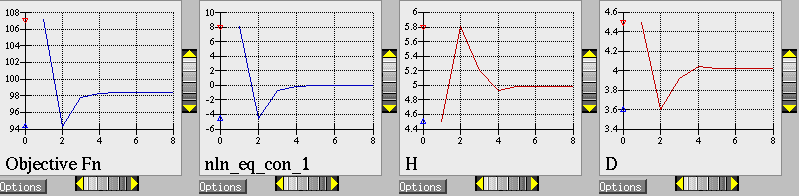
\includegraphics[width=\textwidth]{images/container_graphic}
\caption{Dakota 2D graphics for ``container'' problem showing history of
an objective function, an equality constraint, and two variables.}
\label{output:2dcont}
\end{figure}

The scroll bars which are located on each graph below and to the right
of each plot may be operated by dragging on the bars or pressing the
arrows, both of which result in expansion/contraction of the axis
scale. Clicking on the ``Options'' button results in the window shown
in Figure~\ref{output:2dcontoptions}, which allows the user to include
min/max markers on the vertical axis, vertical and horizontal axis
labels, and a plot legend within the corresponding graphics plot.  In
addition, the values of either or both axes may be plotted using a
logarithmic scale (so long as all plot values are greater than zero)
and an encapsulated postscript (EPS) file, named 
\texttt{dakota\_graphic\_\emph{i}.eps} where \emph{i} is the plot 
window number, can be created using the ``Print'' button.
\begin{figure}
\centering
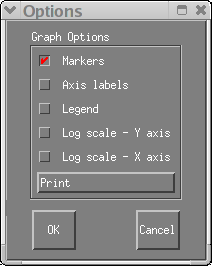
\includegraphics[scale=0.6]{images/container_graphic_options}
\caption{Options for Dakota 2D graphics.}
\label{output:2dcontoptions}
\end{figure}


\section{Error Messages Output}\label{output:error}

A variety of error messages are printed by Dakota in the event that an
error is detected in the input specification. Some of the more common
input errors, and the associated error messages, are described below.
See also the Common Specification Mistakes section in the Dakota
Reference Manual~\cite{RefMan}.

Incorrectly spelled specifications, such as 
\texttt{``numericl\_gradients''}, will result in error messages of the form:
\begin{small}
\begin{verbatim}
    Parser detected syntax error: unrecognized identifier 'numericl_gradients'
      within responses keyword.
    Please refer to the dakota.input.txt distributed with this executable.
\end{verbatim}
\end{small}

The input parser catches syntax errors, but not logic errors. The fact
that certain input combinations are erroneous must be detected after
parsing, at object construction time. For example, if a
\texttt{no\_gradients} specification for a response data set is
combined with selection of a gradient-based optimization method, then
this error must be detected during set-up of the optimizer (see last
line of listing):
\begin{small}
\begin{verbatim}
    Running MPI executable in serial mode.
    Dakota version 4.0 released 05/12/2006.
    Writing new restart file dakota.rst
    Constructing Single Method Strategy...
    methodName = npsol_sqp
    gradientType = none
    hessianType = none

    Error: gradient-based optimizers require a gradient specification.
\end{verbatim}
\end{small}

Another common mistake involves a mismatch between the amount of data
expected on a function evaluation and the data returned by the user's
simulation code or driver. The available response data is specified in
the responses keyword block, and the subset of this data needed for a
particular evaluation is managed by the active set vector. For
example, if Dakota expects function values and gradients to be
returned (as indicated by an active set vector containing 3's), but
the user's simulation code only returns function values, then the
following error message is generated:
\begin{small}
\begin{verbatim}
    At EOF: insufficient data for functionGradient 1
\end{verbatim}
\end{small}

Unfortunately, descriptive error messages are not available for all
possible failure modes of Dakota. If you encounter core dumps,
segmentation faults, or other failures, please request help using the
support mechanisms described on the
\href{http://dakota.sandia.gov/}{Dakota website}.

\section{Variables Output from Pre-run}

The pre-run mode (supported only for select methods) permits
specification of an output file to which Dakota will write parameter
(variables) data in annotated format (see
Section~\ref{input:tabularformat}) with data columns corresponding to
each variable.  This file can be generated with sampling, parameter
study, and DACE methods by invoking
\begin{small}
\begin{verbatim}
    dakota -i dakota.in -pre_run ::variables.dat
\end{verbatim}
\end{small}
for example, to output the variables (samples) in an LHS study.

\chapter{Advanced Simulation Code Interfaces}\label{advint}

\section{Building an Interface to a Engineering Simulation Code}\label{advint:building}

To interface an engineering simulation package to Dakota using one of
the black-box interfaces (system call or fork), pre- and
post-processing functionality typically needs to be supplied (or
developed) in order to transfer the parameters from Dakota to the
simulator input file and to extract the response values of interest
from the simulator's output file for return to Dakota (see
Figures~\ref{intro:bbinterface}
and~\ref{interfaces:bbinterfacecomp}). This is often managed through
the use of scripting languages, such as C-shell~\cite{And86}, Bourne
shell~\cite{Bli96}, Perl~\cite{Wal96}, or Python~\cite{Mar03}. While
these are common and convenient choices for simulation
drivers/filters, it is important to recognize that any executable file
can be used. If the user prefers, the desired pre- and post-processing
functionality may also be compiled or interpreted from any number of
programming languages (C, C++, F77, F95, JAVA, Basic, etc.).

In the \texttt{Dakota/examples/script\_interfaces/generic} directory, a
simple example uses the Rosenbrock test function as a mock engineering
simulation code. Several scripts have been included to demonstrate
ways to accomplish the pre- and post-processing needs. Actual
simulation codes will, of course, have different pre- and
post-processing requirements, and as such, this example serves only to
demonstrate the issues associated with interfacing a
simulator. Modifications will almost surely be required for new
applications.

\subsection{Generic Script Interface Files} 

The {\tt Dakota/generic} directory contains four important files:
\texttt{dakota\_rosenbrock.in} (the Dakota input file),
\texttt{simulator\_script} (the simulation driver script),
\texttt{dprepro} (a pre-processing utility), and \\
\texttt{templatedir/ros.template} (a template simulation input file).

The file \texttt{dakota\_rosenbrock.in} specifies the study that
Dakota will perform and, in the interface section, describes the
components to be used in performing function evaluations. In
particular, it identifies \\ \texttt{simulator\_script} as its
\texttt{analysis\_driver}, as shown in Figure~\ref{advint:figure01}.
\begin{figure}
  \centering
  \begin{bigbox}
    \begin{small}
      \verbatimtabinput[8]{dakota_rosenbrock.in}
    \end{small}
  \end{bigbox}
  \caption{The \texttt{dakota\_rosenbrock.in} input file.}
  \label{advint:figure01}
\end{figure}

The \texttt{simulator\_script} listed in Figure~\ref{advint:figure02}
is a short C-shell driver script that Dakota executes to perform each
function evaluation. The names of the parameters and results files are
passed to the script on its command line; they are
referenced in the script by \texttt{\$argv[1]}
and \texttt{\$argv[2]}, respectively. The \texttt{simulator\_script}
is divided into three parts: pre-processing, analysis, and post-processing.
% is divided into five parts: set up, pre-processing, analysis,
% post-processing, and clean up.

\begin{figure}
  \centering
  \begin{bigbox}
    \begin{small}
      \verbatimtabinput[8]{simulator_script}
    \end{small}
  \end{bigbox}
  \caption{The \texttt{simulator\_script} sample driver script.}
  \label{advint:figure02}
\end{figure}

% The set up portion strips the function evaluation number from
% \texttt{\$argv[1]}and assigns it to the shell variable \texttt{\$num},
% which is then used to create a tagged working directory for a
% particular evaluation. For example, on the first evaluation,
% ``\texttt{1}'' is stripped from ``\texttt{params.in.1}'' in order to
% create ``\texttt{workdir.1}''. The primary reason for creating
% separate working directories is so that the files associated with one
% simulation do not conflict with those for another simulation. This is
% particularly important when executing concurrent simulations in
% parallel (to actually execute function evaluations concurrently,
% uncomment the \texttt{asynchronous} line in \texttt{dakota\_rosenbrock.in}).
% %Once executing within the confines of the working directory, tags on the 
% %files are no longer necessary, and for this reason, the tagged parameters
% %file is moved to a more convenient name of ``\texttt{dakota\_vars}''.

In the pre-processing portion, the \texttt{simulator\_script} uses
\texttt{dprepro}, a parsing utility, to extract the
current variable values from a parameters file (\texttt{\$argv[1]})
and combine them with the simulator template input file
(\texttt{ros.template}) to create a new input file (\texttt{ros.in})
for the simulator. Internal to Sandia, the APREPRO utility is often
used for this purpose. For external sites where APREPRO is not
available, the DPrePro utility mentioned above is an alternative with
many of the capabilities of APREPRO that is specifically tailored for
use with Dakota and is distributed with it (in
\\ \texttt{Dakota/examples/script\_interfaces/generic/dprepro}, or {\tt
Dakota/bin} in a binary distribution).  Additionally, the BPREPRO
utility is another alternative to APREPRO (see~\cite{WalXX}), and at
Lockheed Martin sites, the JPrePost utility is available as a JAVA
pre- and post-processor~\cite{Fla}.  The \texttt{dprepro} script
(usage shown in Figure~\ref{advint:figure03}) will be used here for
simplicity of discussion. It can use either Dakota's \texttt{aprepro}
parameters file format (see
Section~\ref{variables:parameters:aprepro}) or Dakota's standard
format (see Section~\ref{variables:parameters:standard}), so either
option may be selected in the interface section of the Dakota input
file. The \texttt{ros.template} file listed in
Figure~\ref{advint:figure04} is a template simulation input file which
contains targets for the incoming variable values, identified by the
strings ``\texttt{\{x1\}}'' and ``\texttt{\{x2\}}''.  These
identifiers match the variable descriptors specified in
\texttt{dakota\_rosenbrock.in}. The template input file is contrived
as Rosenbrock has nothing to do with finite element analysis; it only
mimics a finite element code to demonstrate the simulator
template process. The \texttt{dprepro} script will search the
simulator template input file for fields marked with curly
brackets and then create a new file (\texttt{ros.in}) by replacing
these targets with the corresponding numerical values for the
variables.  As noted in the usage information for \texttt{dprepro} and
shown in \texttt{simulator\_script}, the names for the Dakota
parameters file (\texttt{\$argv[1]}), template file
(\texttt{ros.template}), and generated input file (\texttt{ros.in})
must be specified in the \texttt{dprepro} command line arguments.

\begin{figure}
  \centering
  \begin{bigbox}
    \begin{small}
      \verbatimtabinput[8]{dprepro_usage}
    \end{small}
  \end{bigbox}
  \caption{Partial listing of the \texttt{dprepro} script.}
  \label{advint:figure03}
\end{figure}

\begin{figure}
  \centering
  \begin{bigbox}
    \begin{small}
      \verbatimtabinput[8]{ros.template}
    \end{small}
  \end{bigbox}
  \caption{Listing of the \texttt{ros.template} file}
  \label{advint:figure04}
\end{figure}

The second part of the script executes the \texttt{rosenbrock\_bb}
simulator. The input and output file names, \texttt{ros.in} and
\texttt{ros.out}, respectively, are hard-coded into the FORTRAN 77
program \texttt{rosenbrock\_bb.f}. When the \texttt{rosenbrock\_bb}
simulator is executed, the values for \texttt{x1} and \texttt{x2} are
read in from \texttt{ros.in}, the Rosenbrock function is evaluated,
and the function value is written out to \texttt{ros.out}.

The third part performs the post-processing and writes the response
results to a file for Dakota to read. Using the UNIX ``\texttt{grep}'' utility, the
particular response values of interest are extracted from the raw
simulator output and saved to a temporary file (\texttt{results.tmp}).
When complete, this file is renamed \texttt{\$argv[2]}, which in this
example is always ``\texttt{results.out}''.
Note that moving or renaming the completed results file
avoids any problems with read race
conditions (see Section~\ref{parallel:SLP:local:system}).

% Finally, in the clean up phase, the working directory is removed to
% reduce the amount of disk storage required to execute the study. If
% data from each simulation needs to be saved, this step can be
% commented out by inserting a ``\texttt{\#}'' character before
% ``\texttt{$\backslash$rm -rf}''.

Because the Dakota input file \texttt{dakota\_rosenbrock.in}
(Figure~\ref{advint:figure01}) specifies
\texttt{work\_directory} and \texttt{directory\_tag} in its interface
section, each invocation of \texttt{simulator\_script} wakes up in
its own temporary directory, which Dakota has populated with the
contents of directory \texttt{templatedir}.  Having a separate directory
for each invocation of \texttt{simulator\_script} simplifies the script
when the Dakota input file specifies \texttt{asynchronous} (so
several instances of \texttt{simulator\_script} might run simultaneously),
as fixed names such as \texttt{ros.in}, \texttt{ros.out}, and \texttt{results.tmp}
can be used for intermediate files.  If neither \texttt{asynchronous} nor
\texttt{file\_tag} is specified, and if there is no need (e.g., for debugging)
to retain intermediate files having fixed names, then \texttt{directory\_tag}
offers no benefit and can be omitted.  An alternative to \texttt{directory\_tag}
is to proceed as earlier versions of this chapter --- prior to Dakota 5.0's
introduction of \texttt{work\_directory} --- recommended:  add two more
steps to the \texttt{simulator\_script},
an initial one to create a temporary directory explicitly and
copy \texttt{templatedir} to it if needed, and a final step to remove the temporary
directory and any files in it.

When \texttt{work\_directory} is specified, Dakota adjusts the \texttt{\$PATH} seen
by \texttt{simulator\_script} so that simple program names
%in the \texttt{simulator\_script}
(i.e., names not containing a slash) that
are visible in Dakota's directory will also be visible in the work directory.
Relative path names ---
involving an intermediate slash but not an initial one,
such as \texttt{./rosenbrock\_bb} or \texttt{a/bc/rosenbrock\_bb} ---
will only be visible in the work directory if a \texttt{template\_directory}
or \texttt{template\_files} specification (see \S\ref{interfaces:workdir})
has made them visible there.

As an example of the data flow on a particular function evaluation,
consider evaluation 60. The parameters file for this evaluation consists of:
\begin{small}
\begin{verbatim}
    { DAKOTA_VARS     =                      2 }
    { x1              =  1.638247697999295e-01 }
    { x2              =  2.197298209103481e-02 }
    { DAKOTA_FNS      =                      1 }
    { ASV_1           =                      1 }
    { DAKOTA_DER_VARS =                      2 }
    { DVV_1           =                      1 }
    { DVV_2           =                      2 }
    { DAKOTA_AN_COMPS =                      0 }
\end{verbatim}
\end{small}

This file is called \texttt{workdir/workdir.60/params.in} if the line
\begin{small}
\begin{verbatim}
 	  named 'workdir' file_save  directory_save
\end{verbatim}
\end{small}
in Figure~\ref{advint:figure01} is uncommented.
The first portion of the file indicates that there are two variables,
followed by new values for variables \texttt{x1} and \texttt{x2}, and
one response function (an objective function), followed by an active
set vector (ASV) value of \texttt{1}. The ASV indicates the need to
return the value of the objective function for these parameters (see
Section~\ref{variables:asv}).  The \texttt{dprepro} script reads the
variable values from this file, namely \texttt{1.638247697999295e-01}
and \texttt{2.197298209103481e-02} for \texttt{x1} and \texttt{x2}
respectively, and substitutes them in the \texttt{\{x1\}} and
\texttt{\{x2\}} fields of the \texttt{ros.template} file. The final
three lines of the resulting input file (\texttt{ros.in}) then appear
as follows:
\begin{small}
\begin{verbatim}
    variable 1 1.638247697999295e-01
    variable 2 2.197298209103481e-02
    end
\end{verbatim}
\end{small}

where all other lines are identical to the template file. The
\texttt{rosenbrock\_bb} simulator accepts \texttt{ros.in} as its input
file and generates the following output to the file \texttt{ros.out}:
\begin{small}
\begin{verbatim}
    Beginning execution of model: Rosenbrock black box
    Set up complete.
    Reading nodes.
    Reading elements.
    Reading materials.
    Checking connectivity...OK
    *****************************************************

    Input value for x1 =  0.1638247697999295E+00
    Input value for x2 =  0.2197298209103481E-01

    Computing solution...Done
    *****************************************************
    Function value =  0.7015563957680092E+00
    Function gradient = [ -0.1353509902591768E+01 -0.9731146217930163E+00 ]
\end{verbatim}
\end{small}

Next, the appropriate values are extracted from the raw simulator output
and returned in the results file. This post-processing is relatively
trivial in this case, and the \texttt{simulator\_script} uses the
\texttt{grep} and \texttt{cut} utilities to extract the value from the
``\texttt{Function value}" line of the \texttt{ros.out} output file and save it to
\texttt{\$argv[2]}, which is the \texttt{results.out} file for this
evaluation. This single value provides the objective function value
requested by the ASV.

After 132 of these function evaluations, the following Dakota output
shows the final solution using the \\ \texttt{rosenbrock\_bb} simulator:
\begin{small}
\begin{verbatim}
    Exit NPSOL - Optimal solution found.

    Final nonlinear objective value =   0.1165704E-06

   NPSOL exits with INFORM code = 0 (see "Interpretation of output" section in NPSOL manual)

   NOTE: see Fortran device 9 file (fort.9 or ftn09)
         for complete NPSOL iteration history.

   <<<<< Iterator npsol_sqp completed.
   <<<<< Function evaluation summary: 132 total (132 new, 0 duplicate)
   <<<<< Best parameters          =
                         9.9965861667e-01 x1
                         9.9931682203e-01 x2
   <<<<< Best objective function  =
                      1.1657044253e-07
   <<<<< Best data captured at function evaluation 130

   <<<<< Iterator npsol_sqp completed.
   <<<<< Single Method Strategy completed.
   Dakota execution time in seconds:
     Total CPU        =       0.12 [parent =   0.116982, child =   0.003018]
     Total wall clock =    1.47497
\end{verbatim}
\end{small}

\subsection{Adapting These Scripts to Another Simulation}

To adapt this approach for use with another simulator, several steps
need to be performed:

\begin{enumerate}
\item Create a template simulation input file by identifying the fields
  in an existing input file that correspond to the variables of
  interest and then replacing them with \texttt{\{\}} identifiers
  (e.g. \texttt{\{cdv\_1\}}, \texttt{\{cdv\_2\}}, etc.) which match
  the Dakota variable descriptors. Copy this template input file to a
  templatedir that will be used to create working directories for the
  simulation.

\item Modify the \texttt{dprepro} arguments in
  \texttt{simulator\_script} to reflect names of the Dakota parameters
  file (previously ``\texttt{\$argv[1]}''), template file name
  (previously ``\texttt{ros.template}'') and generated input file
  (previously ``\texttt{ros.in}''). Alternatively, use APREPRO,
  BPREPRO, or JPrePost to perform this step (and adapt the syntax
  accordingly).

\item Modify the analysis section of \texttt{simulator\_script} to
  replace the \texttt{rosenbrock\_bb} function call with the new
  simulator name and command line syntax (typically including the
  input and output file names).

\item Change the post-processing section in \texttt{simulator\_script}
  to reflect the revised extraction process. At a minimum, this would
  involve changing the \texttt{grep} command to reflect the name of
  the output file, the string to search for, and the characters to cut
  out of the captured output line. For more involved post-processing
  tasks, invocation of additional tools may have to be added to the
  script.

\item Modify the \texttt{dakota\_rosenbrock.in} input file to reflect,
  at a minimum, updated variables and responses specifications.
\end{enumerate}

These nonintrusive interfacing approaches can be used to rapidly
interface with simulation codes. While generally custom for each new
application, typical interface development time is on the order of an
hour or two. Thus, this approach is scalable when dealing with many
different application codes. Weaknesses of this approach include the
potential for loss of data precision (if care is not taken to preserve
precision in pre- and post-processing file I/O), a lack of robustness
in post-processing (if the data capture is too simplistic), and
scripting overhead (only noticeable if the simulation time is on the
order of a second or less).

If the application scope at a particular site is more focused and only
a small number of simulation codes are of interest, then more
sophisticated interfaces may be warranted. For example, the economy of
scale afforded by a common simulation framework justifies additional
effort in the development of a high quality Dakota interface. In these
cases, more sophisticated interfacing approaches could involve a more
thoroughly developed black box interface with robust support of a
variety of inputs and outputs, or it might involve intrusive
interfaces such as the direct simulation interface discussed below in
Section~\ref{advint:direct} or the SAND interface described in
Section~\ref{intro:coupling}.

\subsection{Additional Examples}

A variety of additional examples of black-box interfaces to simulation
codes are maintained in the\\
\texttt{Dakota/examples/script\_interfaces} directory in the source
code distribution.


\section{Developing a Direct Simulation Interface}\label{advint:direct}

If a more efficient interface to a simulation is desired (e.g., to
eliminate process creation and file I/O overhead) or if a targeted
computer architecture cannot accommodate separate optimization and
simulation processes (e.g., due to lightweight operating systems on
compute nodes of large parallel computers), then linking a simulation
code directly with Dakota may be desirable. This is an advanced
capability of Dakota, and it requires a user to have access to (and
knowledge of) the Dakota source code, as well as the source code of
the simulation code.

Three approaches are outlined below for developing direct linking
between Dakota and a simulation: extension, derivation, and
sandwich. For additional information, refer to ``Interfacing with
Dakota as a Library'' in the Dakota Developers Manual~\cite{DevMan}.

Once performed, Dakota can bind with the new direct simulation
interface using the \texttt{direct} interface specification in
combination with an \texttt{analysis\_driver}, \texttt{input\_filter}
or \texttt{output\_filter} specification that corresponds to the name
of the new subroutine.

\subsection{Extension}\label{advint:direct:extension}

The first approach to using the direct function capability with a new
simulation (or new internal test function) involves \emph{extension}
of the existing \textbf{DirectFnApplicInterface} class to include new
simulation member functions.  In this case, the following steps are
performed:
\begin{enumerate}
\item The functions to be invoked (analysis programs, input and
  output filters, internal testers) must have their main programs
  changed into callable functions/subroutines.

\item The resulting callable function can then be added directly
  to the private member functions in \textbf{DirectFnApplicInterface}
  if this function will directly access the Dakota data structures
  (variables, active set, and response attributes of the class). It is
  more common to add a wrapper function to
  \textbf{DirectFnApplicInterface} which manages the Dakota data
  structures, but allows the simulator subroutine to retain a level of
  independence from Dakota (see Salinas, ModelCenter, and Matlab
  wrappers as examples).

\item The if-else blocks in the \textbf{derived\_map\_if()},
  \textbf{derived\_map\_ac()}, and \textbf{derived\_map\_of()} member
  functions of the \textbf{DirectFnApplicInterface} class must be
  extended to include the new function names as options. If the new
  functions are class member functions, then Dakota data access may be
  performed through the existing class member attributes and data
  objects do not need to be passed through the function parameter
  list. In this case, the following function prototype is appropriate:
\begin{small}
\begin{verbatim}
    int function_name();
\end{verbatim}
\end{small}
  If, however, the new function names are not members of the
  \textbf{DirectFnApplicInterface} class, then an \texttt{extern}
  declaration may additionally be needed and the function prototype
  should include passing of the Variables, ActiveSet, and Response
  data members:
\begin{small}
\begin{verbatim}
    int function_name(const Dakota::Variables& vars,
                      const Dakota::ActiveSet& set, Dakota::Response& response);
\end{verbatim}
\end{small}

\item The Dakota system must be recompiled and linked with the new
  function object files or libraries.
\end{enumerate}

Various header files may have to be included, particularly within the
\textbf{DirectFnApplicInterface} class, in order to recognize new
external functions and compile successfully. Refer to the Dakota
Developers Manual~\cite{DevMan} for additional information on the
\textbf{DirectFnApplicInterface} class and the Dakota data types.

\subsection{Derivation}\label{advint:direct:derivation}

As described in ``Interfacing with Dakota as a Library'' in the Dakota
Developers Manual~\cite{DevMan}, a derivation approach can be employed
to further increase the level of independence between Dakota and the
host application.  In this case, rather than \emph{adding} a new
function to the existing \textbf{DirectFnApplicInterface} class, a new
interface class is derived from \textbf{DirectFnApplicInterface} which
\emph{redefines} the \textbf{derived\_map\_if()},
\textbf{derived\_map\_ac()}, and \textbf{derived\_map\_of()} virtual 
functions.

% Note: this approach has benefits primarily in library mode
In the approach of Section~\ref{advint:direct:sandwich} below, the 
class derivation approach avoids the need to recompile the Dakota 
library when the simulation or its direct interface class is modified.

\subsection{Sandwich}\label{advint:direct:sandwich}

In a ``sandwich'' implementation, a simulator provides both the
``front end'' and ``back end'' with Dakota sandwiched in the middle.
To accomplish this approach, the simulation code is responsible for
interacting with the user (the front end), links Dakota in as a
library (refer to ``Interfacing with Dakota as a Library'' in the
Dakota Developers Manual~\cite{DevMan}), and plugs in a derived direct
interface class to provide a closely-coupled mechanism for performing
function evaluations (the back end).  This approach makes Dakota
services available to other codes and frameworks and is currently used
by Sandia codes such as Xyce (electrical simulation), Sage (CFD), and
SIERRA (multiphysics).


\section{Existing Direct Interfaces to External Simulators}\label{advint:existingdirect}

In addition to built-in polynomial test functions described in
Section~\ref{interfaces:direct}, Dakota includes direct interfaces to
Sandia's Salinas code for structural dynamics, Phoenix Integration's
ModelCenter framework, The Mathworks' Matlab scientific computing
environment, Scilab (as described in Section~\ref{scilab}), and
Python.  While these can be interfaced to with a script-based
approach, some usability and efficiency gains may be realized by
re-compiling Dakota with these direct interfaces enabled.  Some
details on Matlab and Python interfaces are provided here.  Note that
these capabilities permit using Matlab or Python to evaluate a
parameter to response mapping; they do not make Dakota algorithms
available as a service, i.e., as a Matlab toolbox or Python module.

\subsection{Matlab}\label{advint:existingdirect:matlab} 

Dakota's direct function interface includes the capability to invoke
Matlab for function evaluations, using the Matlab engine API.  When
using this close-coupling, the Matlab engine is started once when
Dakota initializes, and then during analysis function evaluations are
performed exchanging parameters and results through the Matlab C API.
This eliminates the need to use the file system and the expense of
initializing the Matlab engine for each function evaluation.

The Dakota/Matlab interface has been built and tested on 32-bit Linux
with Matlab 7.0 (R14) and on 64-bit Linux with Matlab 7.1 (R14SP3).
Configuration support for other platforms is included, but is
untested.  Builds on other platforms or with other versions of Matlab
may require modifications to Dakota including its build system

To use the Dakota/Matlab interface, Dakota must be configured and
compiled with the Matlab feature enabled.  The Mathworks only provides
shared object libraries for its engine API, so Dakota must be
dynamically linked to at least the Matlab libraries.  To compile
Dakota with the Matlab interface enabled, set the CMake variable {\tt
  DAKOTA\_MATLAB:BOOL=ON}, possibly with {\tt
  MATLAB\_DIR:FILEPATH=/path/to/matlab}, where \\ {\tt MATLAB\_DIR} is the
root of your Matlab installation (it should be a directory containing
directories bin/YOURPLATFORM and extern/include).

Since the Matlab libraries are linked dynamically, they must be
accessible at compile time and at run time. Make sure the path to the
appropriate Matlab shared object libraries is on your 
{\tt LD\_LIBRARY\_PATH}.  For example to accomplish this in BASH on
32-bit Linux, one might type
\begin{verbatim}
export LD_LIBRARY_PATH=/usr/local/matlab/bin/glnx86:$LD_LIBRARY_PATH
\end{verbatim} %$
or add such a command to the .bashrc file.  Then proceed with
compiling as usual.

Example files corresponding to the following tutorial are available in \\ 
{\tt Dakota/examples/linked\_interfaces/Matlab}.

\subsubsection{Dakota/Matlab input file specification}

The Matlab direct interface is specified with {\tt direct, matlab}
keywords in an interface specification.  The Matlab m-file which
performs the analysis is specified through the {\tt analysis\_drivers}
keyword.  Here is a sample Dakota {\tt interface} specification:
\begin{small}
\begin{verbatim}
  interface,
    matlab
      analysis_drivers = 'myanalysis.m'
\end{verbatim} 
\end{small}

Multiple Matlab analysis drivers are supported.  Multiple analysis
components are supported as for other interfaces as described in
Section~\ref{interfaces:components}.  The {\tt .m} extension in the
{\tt analysis\_drivers} specification is optional and will be stripped
by the interface before invoking the function.  So {\tt myanalysis}
and {\tt myanalysis.m} will both cause the interface to attempt to
execute a Matlab function {\tt myanalysis} for the evaluation.

\subsubsection{Matlab .m file specification}

The Matlab analysis file {\tt myanalysis.m} must define a Matlab
function that accepts a Matlab structure as its sole argument and
returns the same structure in a variable called {\tt Dakota}.  A
manual execution of the call to the analysis in Matlab should
therefore look like:
\begin{small}
\begin{verbatim}
  >> Dakota = myanalysis(Dakota)
\end{verbatim} 
\end{small}
Note that the structure named Dakota will be pushed into the Matlab
workspace before the analysis function is called.  The structure
passed from Dakota to the analysis m-function contains essentially the
same information that would be passed to a Dakota direct function
included in {\tt DirectApplicInterface.C}, with fields shown in
Figure~\ref{advint:figure:matlabparams}.

\begin{figure}
\centering
\begin{bigbox}
\begin{small}
\begin{verbatim}
Dakota.
  numFns              number of functions (responses, constraints)
  numVars             total number of variables
  numACV              number active continuous variables
  numADIV             number active discrete integer variables
  numADRV             number active discrete real variables
  numDerivVars        number of derivative variables specified in directFnDVV
  xC                  continuous variable values ([1 x numACV]) 
  xDI                 discrete integer variable values ([1 x numADIV])
  xDR                 discrete real variable values ([1 x numADRV])
  xCLabels            continuous var labels (cell array of numACV strings)
  xDILabels           discrete integer var labels (cell array of numADIV strings)
  xDRLabels           discrete real var labels (cell array of numADIV strings)
  directFnASV         active set vector ([1 x numFns])
  directFnDVV         derivative variables vector ([1 x numDerivVars])
  fnFlag              nonzero if function values requested
  gradFlag            nonzero if gradients requested
  hessFlag            nonzero if hessians requested
  currEvalId          current evaluation ID
\end{verbatim}
\end{small}
\end{bigbox}
\caption{Dakota/Matlab parameter data
structure.\label{advint:figure:matlabparams}}
\end{figure}

The structure {\tt Dakota} returned from the analysis must contain a
subset of the fields shown in
Figure~\ref{advint:figure:matlabresponse}.  It may contain additional
fields and in fact is permitted to be the structure passed in,
augmented with any required outputs.
\begin{figure} \centering
\begin{bigbox}
\begin{small}
\begin{verbatim}
Dakota.
  fnVals      ([1 x numFns], required if function values requested)
  fnGrads     ([numFns x numDerivVars], required if gradients  requested)
  fnHessians  ([numFns x numDerivVars x numDerivVars], 
               required if hessians requested)
  fnLabels    (cell array of numFns strings, optional)
  failure     (optional: zero indicates success, nonzero failure
\end{verbatim}
\end{small}
\end{bigbox}
\caption{Dakota/Matlab response data
structure.\label{advint:figure:matlabresponse}}
\end{figure}

An example Matlab analysis driver {\tt rosenbrock.m} for the
Rosenbrock function is shown in Figure
~\ref{advint:figure:matlabrosen}.
\begin{figure} \centering
\begin{bigbox}
\begin{tiny}
\begin{verbatim}
function Dakota = rosenbrock(Dakota)

  Dakota.failure = 0;

  if ( Dakota.numVars ~= 2 | Dakota.numADV | ...
      ( ~isempty( find(Dakota.directFnASM(2,:)) | ...
      find(Dakota.directFnASM(3,:)) ) & Dakota.numDerivVars ~= 2 ) )
    
    sprintf('Error: Bad number of variables in rosenbrock.m fn.\n');
    Dakota.failure = 1;

  elseif (Dakota.numFns > 2) 
  
    % 1 fn -> opt, 2 fns -> least sq
    sprintf('Error: Bad number of functions in rosenbrock.m fn.\n');
    Dakota.failure = 1;

  else
 
    if Dakota.numFns > 1 
      least_sq_flag = true;
    else
      least_sq_flag = false;
    end

    f0 = Dakota.xC(2)-Dakota.xC(1)*Dakota.xC(1);
    f1 = 1.-Dakota.xC(1);
  
    % **** f:
    if (least_sq_flag) 
      if Dakota.directFnASM(1,1)
        Dakota.fnVals(1) = 10*f0;
      end
      if Dakota.directFnASM(1,2)
        Dakota.fnVals(2) = f1;
      end
    else
      if Dakota.directFnASM(1,1)
        Dakota.fnVals(1) = 100.*f0*f0+f1*f1;
      end
    end
  
    % **** df/dx:
    if (least_sq_flag)
      if Dakota.directFnASM(2,1)
        Dakota.fnGrads(1,1) = -20.*Dakota.xC(1);
        Dakota.fnGrads(1,2) =  10.;
      end
      if Dakota.directFnASM(2,2)
        Dakota.fnGrads(2,1) = -1.;
        Dakota.fnGrads(2,2) =  0.;
      end
  
    else 
  
      if Dakota.directFnASM(2,1)
        Dakota.fnGrads(1,1) = -400.*f0*Dakota.xC(1) - 2.*f1;
        Dakota.fnGrads(1,2) =  200.*f0;
      end
      
    end

    % **** d^2f/dx^2:
    if (least_sq_flag)
     
      if Dakota.directFnASM(3,1)
        Dakota.fnHessians(1,1,1) = -20.;
        Dakota.fnHessians(1,1,2) = 0.;
        Dakota.fnHessians(1,2,1) = 0.;
        Dakota.fnHessians(1,2,2) = 0.;
      end
      if Dakota.directFnASM(3,2)
        Dakota.fnHessians(2,1:2,1:2) = 0.;
      end
      
    else
    
      if Dakota.directFnASM(3,1) 
        fx = Dakota.xC(2) - 3.*Dakota.xC(1)*Dakota.xC(1);
        Dakota.fnHessians(1,1,1) = -400.*fx + 2.0;
        Dakota.fnHessians(1,1,2) = -400.*Dakota.xC(1); 
        Dakota.fnHessians(1,2,1) = -400.*Dakota.xC(1);
        Dakota.fnHessians(1,2,2) =  200.;
      end
    
    end
  
    Dakota.fnLabels = {'f1'};
   
  end
\end{verbatim}
\end{tiny}
\end{bigbox}
\caption{Sample Matlab implementation of the Rosenbrock test function
for the Dakota/Matlab interface.\label{advint:figure:matlabrosen}}
\end{figure}

\subsection{Python}\label{advint:existingdirect:python} 

Dakota's Python direct interface has been tested on Linux with Python
2.x.  When enabled, it allows Dakota to make function evaluation calls
directly to an analysis function in a user-provided Python module.
Data may flow between Dakota and Python either in multiply-subscripted
lists or NumPy arrays.

The Python direct interface must be enabled when compiling Dakota.
Set the CMake variable \\ {\tt DAKOTA\_PYTHON:BOOL=ON}, and optionally
{\tt Dakota\_PYTHON\_NUMPY:BOOL=ON} to use Dakota's NumPy array
interface (requires arrayobject.h).  If NumPy is not enabled, Dakota
will use multiply-subscripted lists for data flow.

An example of using the Python direct interface with both lists and
arrays is included in \\
{\tt examples/linked\_interfaces/Python}.  The Python direct driver is
selected with, for example,
\begin{verbatim}
  interface,
    python
      analysis_drivers = 'python_module:analysis_function'
\end{verbatim}
where {\tt python\_module} denotes the module (file {\tt
python\_module.py}) Dakota will attempt to import into the Python
environment and {\tt analysis\_function} denotes the function to call
when evaluating a parameter set.  It is likely necessary to set the
{\tt PYTHONPATH} environment variable to include the location of the
Python module you wish to load.

Whether using the list or array interface, data from Dakota is passed
(via kwargs) into the user function in a dictionary containing the
entries shown in Table~\ref{advint:table:pythonparams}.  The {\tt
analysis\_function} must return a dictionary containing the data
specified by the active set vector with fields ``fns'', ``fnGrads'',
and ``fnHessians'', corresponding to function values, gradients, and
Hessians, respectively.  The function may optionally include a failure
code in ``failure'' (zero indicates success, nonzero failure) and
function labels in ``fnLabels''.  See the linked interfaces example
referenced above for more details.

\begin{table}
\centering
\caption{Data dictionary passed to Python direct interface.}
\label{advint:table:pythonparams}\vspace{2mm}
\begin{tabular}{|l|l|}
\hline
\textbf{Entry Name} & \textbf{Description}  \\
\hline
functions  & number of functions (responses, constraints) \\
variables  & total number of variables \\
cv         & list/array of continuous variable values \\
div        & list/array of discrete integer variable values \\
drv        & list/array of discrete real variable values \\
av         & single list/array of all variable values \\
cv\_labels  & continuous variable labels \\
div\_labels & discrete integer variable labels \\
drv\_labels & discrete real variable labels \\
av\_labels  & all variable labels \\
asv        & active set vector \\
dvv        & derivative variables vector \\
currEvalId & current evaluation ID number \\
\hline
\end{tabular}
\end{table}

\section{Scilab Script and Direct Interfaces}\label{scilab}

Scilab is open source computation software which can be used to
perform function evaluations during Dakota studies, for example to
calculate the objective function in optimization.  Dakota includes
three Scilab interface variants: scripted, linked, and compiled.  In
each mode, Dakota calls Scilab to perform a function evaluation and
then retrieves the Scilab results.  Dakota's Scilab interface was
contributed in 2011 by Yann Collette and Yann Chapalain.  The
Dakota/Scilab interface variants are described next.

\subsection{Scilab Script Interface} 

Dakota distributions include a directory
\texttt{examples/script\_interfaces/Scilab} which demonstrates
script-based interfacing to Scilab.  The {\tt Rosenbrock} subdirectory
contains four notable files:
\begin{itemize}
  \item \texttt{dakota\_scilab\_rosenbrock.in} (the Dakota input file),
  \item \texttt{rosenbrock.sci} (the Scilab computation code),
  \item \texttt{scilab\_rosen\_bb\_simulator.sh} (the analysis driver), and
  \item \texttt{scilab\_rosen\_wrapper.sci} (Scilab script).
\end{itemize}

The \texttt{dakota\_scilab\_rosenbrock.in} file specifies the Dakota
study to perform.  The interface type is external ({\tt fork}) and the
shell script \texttt{scilab\_rosen\_bb\_simulator.sh} is the analysis
driver used to perform function evaluations.

The Scilab file \texttt{rosenbrock.sci} accepts variable values and
computes the objective, gradient, and Hessian values of the Rosenbrock
function as requested by Dakota.

The \texttt{scilab\_rosen\_bb\_simulator.sh} is a short shell driver
script, like that described in Section~\ref{advint:building}, that
Dakota executes to perform each function evaluation. Dakota passes
the names of the parameters and results files to this script as
\texttt{\$argv[1]} and \texttt{\$argv[2]}, respectively. The
\texttt{scilab\_rosen\_bb\_simulator.sh} is divided into three parts:
pre-processing, analysis, and post-processing.

In the analysis portion, the \texttt{scilab\_rosen\_bb\_simulator.sh}
uses \texttt{scilab\_rosen\_wrapper.sci} to extract the current
variable values from the input parameters file (\texttt{\$argv[1]})
and communicate them to the computation code in
\texttt{rosenbrock.sci}.  The resulting objective function is
transmitted to Dakota via the output result file (\texttt{\$argv[1]}),
and the driver script cleans up any temporary files.

The directory also includes PID and FemTRUSS examples, which are run
in a similar way.

\subsection{Scilab Linked Interface} 

The Dakota/Scilab linked interface allows Dakota to communicate
directly with Scilab through in-memory data structures, typically
resulting in faster communication, as it does not rely on files or
pipes.  In this mode, Dakota publishes a data structure into the
Scilab workspace, and then invokes the specified Scilab
analysis\_driver directly.  In Scilab, this structure is an mlist
(\url{http://help.scilab.org/docs/5.3.2/en\_US/mlist.html}), with the same
fields as in the Matlab interface~\ref{advint:figure:matlabparams},
with the addition of a field {\tt dakota\_type}, which is used to validate
the names of fields in the data structure.

The linked interface is implemented in source files {\tt
  src/ScilabInterface.[CH]} directory, and must be enabled at compile
time when building Dakota from source by setting {\tt
  DAKOTA\_SCILAB:BOOL=ON}, and setting appropriate environment
variables at compile and run time as described in {\tt README.Scilab}
in \\ {\tt examples/linked\_interfaces/Scilab/}.  This directory also
contains examples for the Rosenbrock and PID problems.

These examples are similar to those in {\tt script\_interfaces}, with
a few notable exceptions:
\begin{enumerate}
\item There is no shell driver script
\item The Dakota input file specifies the interface as 'scilab',
  indicating a direct, internal interface to Scilab using the Dakota
  data structure described above:
\begin{small}
\begin{verbatim}
interface,
  scilab
    analysis_driver = 'rosenbrock.sci'
\end{verbatim} 
\end{small}
\end{enumerate}


\subsection{Scilab Compiled Interface} 

In ``compiled interface'' mode, the Dakota analysis driver is a
lightweight shim, which communicates with the running application code
such as Scilab via named pipes.  It is similar to that for Matlab in
\texttt{examples/compiled\_interfaces/Matlab}, whose README is likely
instructive.  An example of a Scilab compiled interface is included in \\
\texttt{examples/compiled\_interfaces/Scilab/Rosenbrock}.

As with the other Scilab examples, there are computation code and
Dakota input files.  Note the difference in the Dakota input file
\texttt{rosenbrock.in}, where the analysis driver starts the dakscilab
shim program and always evaluates functions, gradients, and Hessians.

\begin{small}
\begin{verbatim}
interface,
  fork
    analysis_driver = '../dakscilab -d -fp "exec fp.sci" -fpp "exec fpp.sci"'
    parameters_file = 'r.in'
    results_file = 'r.out'
    deactivate active_set_vector
\end{verbatim} 
\end{small}

The dakscilab executable results from compiling \texttt{dakscilab.c}
and has the following behavior and options.  The driver dakscilab
launches a server.  This server then facilitates communication between
Dakota and Scilab via named pipes communication. The user can also use
the first named pipe (\texttt{\$\{DAKSCILAB\_PIPE\}1}) to communicate
with the server:
\begin{small}
\begin{verbatim}
    echo dbg scilab_script.sce > ${DAKSCILAB_PIPE}1
    echo quit > ${DAKSCILAB_PIPE}1
\end{verbatim} 
\end{small}
The first command, with the keyword 'dbg', launches the script
scilab\_script.sci for evaluation in Scilab.  It permits to give
instructions to Scilab. The second command 'quit' stops the server.

The dakscilab shim supports the following options for the driver call:
\begin{enumerate}
  \item -s  to start the server
  \item -si to run an init script
  \item -sf to run a final script
  \item -f -fp -fpp to specify names of objective function, gradient
    and hessian, then load them.
\end{enumerate}

For the included PID example, the driver call is 
\begin{small}
\begin{verbatim}
    analysis_driver = '../dakscilab -d -si "exec init_test_automatic.sce;"
                     -sf "exec visualize_solution.sce;" -f "exec f_pid.sci"'
\end{verbatim}
\end{small}

Here there is an initialization script
(\texttt{init\_test\_automatic.sce;}) which is launched before the
main computation.  It initializes a specific Scilab module called
xcos. A finalization script to visualize the xcos solution is also
specified (\texttt{visualize\_solution.sce}). Finally, the objective
function is given with the computation code called
\texttt{f\_pid.sci}.


% LocalWords:  Scilab Yann Collette Chapalain Rosenbrock subdirectory dakota bb
% LocalWords:  scilab rosenbrock rosen argv pre PID FemTRUSS workspace mlist 1i
% LocalWords:  Matlab src ScilabInterface BOOL README dakscilab Hessians dbg si
% LocalWords:  init fp fpp sce xcos pid


\chapter{Parallel Computing}\label{parallel}


\section{Overview}\label{parallel:overview}

This chapter describes the various parallel computing capabilities
provided by DAKOTA.  The range of capabilities is extensive and can be
daunting at first; therefore, this chapter takes an incremental
approach in first describing the simplest single-level parallel
computing models (Section~\ref{parallel:SLP}) using asynchronous
local, message passing, and hybrid approaches.  More advanced uses of
DAKOTA can build on this foundation to exploit multiple levels of
parallelism, as described in Section~\ref{parallel:MLP}.  The chapter
concludes with a discussion of using DAKOTA with applications that run
as independent MPI processes (parallel application tiling, for example
on a large compute cluster).  This last section is a good quick start
for interfacing DAKOTA to your parallel (or serial) application on a
cluster.

%In the following sections, the parallel algorithms available in this
%DAKOTA release are listed followed by descriptions of the software
%components that enable parallelism, approaches for utilizing these
%components, and input specification and execution details for running
%parallel DAKOTA studies.


\subsection{Categorization of parallelism}\label{parallel:overview:cat}

To understand the parallel computing possibilities, it is instructive
to first categorize the opportunities for exploiting parallelism into
four main areas~\cite{Eld98a}, consisting of coarse-grained and
fine-grained parallelism opportunities within algorithms and their
function evaluations:

\begin{enumerate}
\item \emph{Algorithmic coarse-grained parallelism}: This parallelism
  involves the concurrent execution of independent function
  evaluations, where a ``function evaluation'' is defined as a data
  request from an algorithm (which may involve value, gradient, and
  Hessian data from multiple objective and constraint functions). This
  concept can also be extended to the concurrent execution of multiple
  ``iterators'' within a ``strategy.'' Examples of algorithms
  containing coarse-grained parallelism include:
  \begin{itemize}
  \item \emph{Gradient-based algorithms}: finite difference gradient
    evaluations, speculative optimization, parallel line search.

  \item \emph{Nongradient-based algorithms}: genetic algorithms (GAs),
    pattern search (PS), Monte Carlo sampling.

  \item \emph{Approximate methods}: design of computer experiments for
    building surrogate models.

  \item \emph{Concurrent-iterator strategies}: optimization under
    uncertainty, branch and bound, multi-start local search, Pareto
    set optimization, island-model GAs.
  \end{itemize}

\item \emph{Algorithmic fine-grained parallelism}: This involves
  computing the basic computational steps of an optimization algorithm
  (i.e., the internal linear algebra) in parallel. This is primarily
  of interest in large-scale optimization problems and simultaneous
  analysis and design (SAND).

\item \emph{Function evaluation coarse-grained parallelism}: This
  involves concurrent computation of separable parts of a single
  function evaluation. This parallelism can be exploited when the
  evaluation of the response data set requires multiple independent
  simulations (e.g. multiple loading cases or operational
  environments) or multiple dependent analyses where the coupling is
  applied at the optimizer level (e.g., multiple disciplines in the
  individual discipline feasible formulation~\cite{Den94a}).

\item \emph{Function evaluation fine-grained parallelism}: This
  involves parallelization of the solution steps within a single
  analysis code.  The DOE laboratories have developed parallel
  analysis codes in the areas of nonlinear mechanics, structural
  dynamics, heat transfer, computational fluid dynamics, shock
  physics, and many others.
\end{enumerate}

By definition, coarse-grained parallelism requires very little
inter-processor communication and is therefore ``embarrassingly
parallel,'' meaning that there is little loss in parallel efficiency
due to communication as the number of processors increases. However,
it is often the case that there are not enough separable computations
on each algorithm cycle to utilize the thousands of processors
available on MP machines. For example, a thermal safety
application~\cite{Eld96a} demonstrated this limitation with a pattern
search optimization in which the maximum speedup exploiting
\emph{only} coarse-grained algorithmic parallelism was shown to be
limited by the size of the design problem (coordinate pattern search
has at most $2n$ independent evaluations per cycle for $n$ design
variables).

Fine-grained parallelism, on the other hand, involves much more
communication among processors and care must be taken to avoid the
case of inefficient machine utilization in which the communication
demands among processors outstrip the amount of actual computational
work to be performed. For example, a chemically-reacting flow
application~\cite{Eld98a} illustrated this limitation for a simulation
of fixed size in which it was shown that, while simulation run time
did monotonically decrease with increasing number of processors, the
relative parallel efficiency $\hat{E}$ of the computation for fixed
model size decreased rapidly (from $\hat{E} \approx 0.8$ at 64
processors to $\hat{E} \approx 0.4$ at 512 processors). This was due
to the fact that the total amount of computation was approximately
fixed, whereas the communication demands were increasing rapidly with
increasing numbers of processors. Therefore, there is a practical
limit on the number of processors that can be employed for
fine-grained parallel simulation of a particular model size, and only
for extreme model sizes can thousands of processors be efficiently
utilized in studies exploiting fine-grained parallelism alone.

These limitations point us to the exploitation of multiple levels of
parallelism, in particular the combination of coarse-grained and
fine-grained approaches. This will allow us to execute fine-grained
parallel simulations on sets of processors where they are most
efficient and then replicate this efficiency with many coarse-grained
instances.  From a software perspective, coarse-grained parallelism by
itself (many instances of a single-processor simulation) and
fine-grained parallelism by itself (a single instance of a large
multiprocessor simulation) can be considered to cover two ends of a
spectrum, and we are interested in also supporting anywhere in between
(any number of instances of any size simulation).  Single-level
parallelism approaches are described in Section~\ref{parallel:SLP},
and multilevel parallelism approaches are discussed in
Section~\ref{parallel:MLP}.

The available concurrency in function evaluation parallelism is
determined by the aspects of a particular systems analysis
application, and is therefore highly application-dependent.
Algorithmic parallelism, on the other hand, is largely determined by
the selection and configuration of a particular algorithm.  These
selection possibilities within DAKOTA are outlined in the following
section.


\subsection{Parallel DAKOTA algorithms} \label{parallel:algorithms}

In DAKOTA, the following parallel algorithms, comprised of iterators
and strategies, provide support for coarse-grained algorithmic
parallelism.  Note that, even if a particular algorithm is serial in
terms of its data request concurrency, other concurrency sources
(e.g., function evaluation coarse-grained and fine-grained
parallelism) may still be available.

\subsubsection{Parallel iterators}\label{parallel:algorithms:iterators}

\begin{itemize}
\item Gradient-based optimizers: CONMIN, DOT, NLPQL, NPSOL, and OPT++
  can all exploit parallelism through the use of DAKOTA's native finite
  differencing routine (selected with \texttt{method\_source dakota}
  in the responses specification), which will perform concurrent
  evaluations for each of the parameter offsets. For \texttt{n}
  variables, forward differences result in an $n+1$ concurrency and
  central differences result in a $2n+1$ concurrency. In addition,
  CONMIN, DOT, and OPT++ can use speculative gradient
  techniques~\cite{Byr88} to obtain better parallel load balancing. By
  speculating that the gradient information associated with a given
  line search point will be used later and computing the gradient
  information in parallel at the same time as the function values, the
  concurrency during the gradient evaluation and line search phases
  can be balanced. NPSOL does not use speculative gradients since this
  approach is superseded by NPSOL's gradient-based line search in
  user-supplied derivative mode.  NLPQL also supports a distributed
  line search capability for generating concurrency~\cite{Sch04}.

\item Nongradient-based optimizers: HOPSPACK, JEGA methods, and most
  SCOLIB methods support parallelism.  HOPSPACK and SCOLIB methods
  exploit parallelism through the use of DAKOTA's concurrent function
  evaluations; however, there are some limitations on the levels of
  concurrency and asynchrony that can be exploited.  These are detailed
  in the DAKOTA Reference Manual. Serial SCOLIB methods include
  Solis-Wets (\texttt{coliny\_solis\_wets}) and certain
  \texttt{exploratory\_moves} options (\texttt{adaptive\_pattern} and
  \texttt{multi\_step}) in pattern search
  (\texttt{coliny\_pattern\_search}).  OPT++ PDS (\texttt{optpp\_pds})
  and NCSU DIRECT (\texttt{ncsu\_direct}) are also currently serial
  due to incompatibilities in DAKOTA and OPT++/NCSU parallelism
  models.  Finally, \texttt{coliny\_pattern\_search} and
  \texttt{asynch\_pattern\_search} support dynamic job queues managed
  with nonblocking synchronization.

\item Least squares methods: in an identical manner to the
  gradient-based optimizers, NL2SOL, NLSSOL, and Gauss-Newton can
  exploit parallelism through the use of DAKOTA's native finite
  differencing routine. In addition, NL2SOL and Gauss-Newton can use
  speculative gradient techniques to obtain better parallel load
  balancing. NLSSOL does not use speculative gradients since this
  approach is superseded by NLSSOL's gradient-based line search in
  user-supplied derivative mode.

\item Surrogate-based minimizers: \texttt{surrogate\_based\_local},
  \texttt{surrogate\_based\_global}, and \texttt{efficient\_global}
  all support parallelism in the initial surrogate construction, but
  subsequent concurrency varies.  In the case of
  \texttt{efficient\_global}, only a single point is generated for
  evaluation for each subsequent cycle and there is no derivatove
  concurrency for this point.  In the case of
  \texttt{surrogate\_based\_local}, only a single point is generated
  per subsequent cycle, but derivative concurrency for numerical
  gradient or Hessian evaluations may be available.  And in the case
  of \texttt{surrogate\_based\_global}, multiple points may be
  generated on each subsequent cycle, depending on the multipoint
  return capability of specific minimizers.

\item Parameter studies: all parameter study methods (\texttt{vector},
  \texttt{list}, \texttt{centered}, and \texttt{multidim}) support
  parallelism. These methods avoid internal synchronization points, so
  all evaluations are available for concurrent execution.

\item Design of experiments: all \texttt{dace} (\texttt{grid},
  \texttt{random}, \texttt{oas}, \texttt{lhs}, \texttt{oa\_lhs},
  \texttt{box\_behnken}, and \texttt{central\_composite}),
  \texttt{fsu\_quasi\_mc} (\texttt{halton} and \texttt{hammersley}),
  \texttt{fsu\_cvt}, and \texttt{psuade\_moat} methods support
  parallelism.

\item Uncertainty quantification: all nondeterministic methods
  (\texttt{sampling}, \texttt{local\_reliability},
  \texttt{global\_reliability}, \texttt{polynomial\_chaos},
  \texttt{stoch\_collocation},\texttt{local\_interval\_est}, 
  \texttt{global\_interval\_est},\texttt{local\_evidence} and 
  \texttt{global\_evidence})
  support parallelism. In the case of
  \texttt{local\_reliability}, gradient-based optimization is
  involved and parallelism can be exploited through the use of
  DAKOTA's native finite differencing routine.  In the case of
  \texttt{global\_reliability}, EGRA methods support parallelism
  in the initial surrogate construction, but subsequently only
  generate a single point for evaluation per cycle.
\end{itemize}

\subsubsection{Parallel strategies}\label{parallel:algorithms:strategies}

Certain strategies support concurrency in multiple iterator
executions. Currently, the strategies which can exploit this level of
parallelism are:

\begin{itemize}
\item Hybrid minimization: when the sequential hybrid transfers multiple
solution points between methods, single-point minimizers will be executed
concurrently using each of the transferred solution points.

%\item Branch and bound: optimization strategy for mixed-integer nonlinear
%programming with noncategorical discrete variables.

\item Pareto-set optimization: multiobjective optimization strategy for
computing sets of points on the Pareto front of nondominated solutions.

\item Multi-start iteration: strategy for executing multiple instances
of an iterator from different starting points.
\end{itemize}

In the branch and bound case, the available iterator concurrency grows
as the tree develops more branches, so some of the iterator servers
may be idle in the initial phases. Similarly, hybrid minimization will
display varying levels of iterator concurrency based on differing
support of multipoint solution input/output between iterators;
however, the use of multiple parallel configurations among the iterator
sequence should prevent parallel inefficiencies.  Finally, pareto-set
and multi-start have a fixed set of jobs to perform and should exhibit
good load balancing.

\subsubsection{Parallel models}\label{parallel:algorithms:models}

Parallelism support in model classes (see Chapter~\ref{models}) is an
important issue for variable scaling (see
Section~\ref{opt:additional:scaling}) and advanced model recursions
such as surrogate-based minimization, optimization under uncertainty,
and second-order probability (see Chapters~\ref{sbm}
and~\ref{adv_models}).  Support is as follows:

\begin{itemize}
\item Single model: parallelism is managed by the singe interface instance.

\item Recast model: most parallelism is forwarded on to the sub-model.
An exception to this is finite differencing in the presence of
variable scaling.  Since it is desirable to perform offsets in the
scaled space (and avoid minimum step size tolerances), this
parallelism is not forwarded to the sub-model, instead being enacted
at the recast level.

\item Data fit surrogate model: parallelism is supported in the
construction of global surrogate models via the concurrent evaluation
of points generated by design of experiments methods.  Local and
multipoint approximations evaluate only a single point at a time, so
concurrency is available only from any numerical differencing required
for gradient and Hessian data.  Since the top-level iterator is
interfaced only with the (inexpensive) surrogate, no parallelism is
exploited here.  Load balancing can be an important issue when
performing evaluations for update of existing surrogate models.

\item Hierarchical surrogate model: parallelism is supported for both
the low and high fidelity models.  Since the top-level iterator is
interfaced only with the low-fidelity model, and the high-fidelity
model is used only for verifications and correction updating, the
algorithmic coarse-grained parallelism supported by the iterator is
enacted on the low fidelity model and the only parallelism available
for high fidelity executions arises from any numerical differencing
required for high-fidelity gradient and Hessian data.

\item Nested model: Currently, nested models only support concurrency
in the sub-iterator execution on the sub-model.  This means that the
top-level iterator interfaced with the nested model is serialized.  In
future releases, concurrency will be supported at this top level,
allowing techniques such as optimization under uncertainty and
second-order probability (see Section~\ref{models:nested}) to support
concurrent iterator parallelism.
\end{itemize}


\section{Single-level parallelism} \label{parallel:SLP}


DAKOTA's parallel facilities support a broad range of computing
hardware, from custom massively parallel supercomputers on the high
end, to clusters and networks of workstations (NOWs) in the middle
range, to desktop multiprocessors on the low end. Given the reduced
scale in the middle to low ranges, it is more common to exploit only
one of the levels of parallelism; however, this can still be quite
effective in reducing the time to obtain a solution.  Three
single-level parallelism models will be discussed, and are depicted
in Figure~\ref{parallel:figure03}:

\begin{figure}[ht]
  \centering
  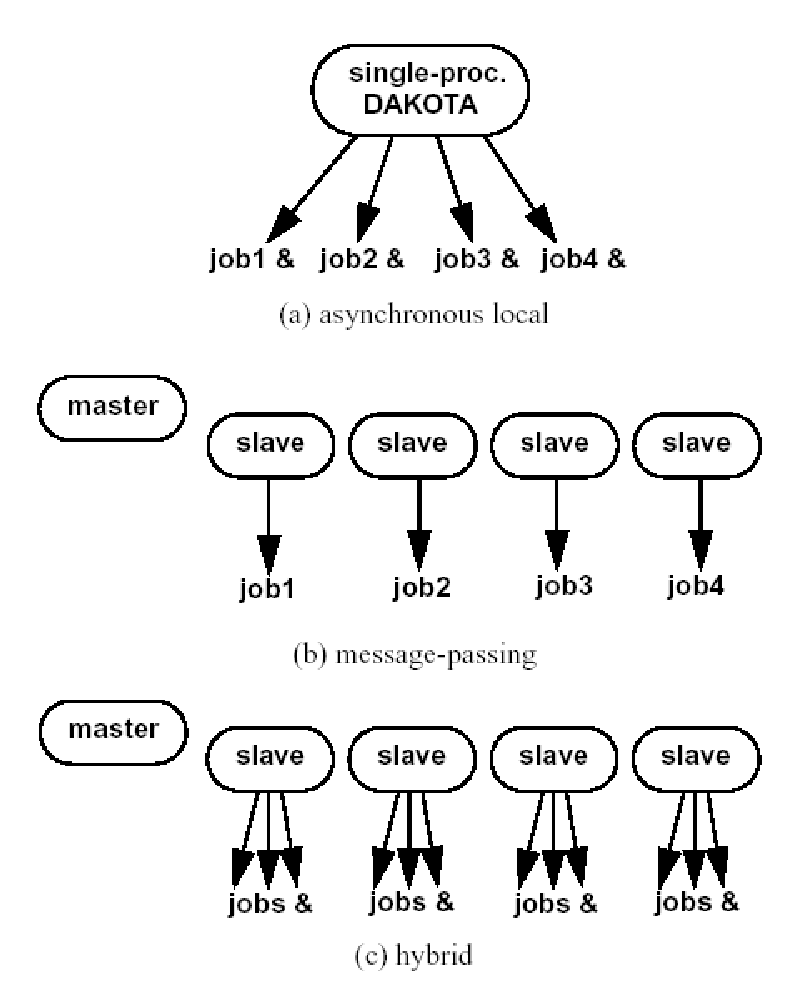
\includegraphics[width=60mm]{images/ex_in_hy_job_management}
  \caption{External, internal, and hybrid job management.}
  \label{parallel:figure03}
\end{figure}

\begin{itemize}
\item \emph{asynchronous local}: DAKOTA executes on a single processor,
but launches multiple jobs concurrently using asynchronous job launching
techniques.

\item \emph{message passing}: DAKOTA executes in parallel using message
passing to communicate between processors.  A single job is launched
per processor using synchronous job launching techniques.

\item \emph{hybrid}: a combination of message passing and asynchronous
local.  DAKOTA executes in parallel across multiple processors and
launches concurrent jobs on each processor.
\end{itemize}

In each of these cases, jobs are executing concurrently and must be
collected in some manner for return to an algorithm.  Blocking and
nonblocking approaches are provided for this, where the blocking
approach is used in most cases:
\begin{itemize}
\item \emph{blocking synchronization}: all jobs in the queue are
completed before exiting the scheduler and returning the set of
results to the algorithm.  The job queue fills and then empties
completely, which provides a synchronization point for the algorithm.

\item \emph{nonblocking synchronization}: the job queue is dynamic,
with jobs entering and leaving continuously.  There are no defined
synchronization points for the algorithm, which requires specialized
algorithm logic (only currently supported by
\texttt{coliny\_pattern\_search} and \texttt{asynch\_pattern\_search}, which
are sometimes referred to as ``fully asynchronous'' algorithms).
\end{itemize}

Given these job management capabilities, it is worth noting that the
popular term ``asynchronous'' can be ambiguous when used in isolation.
In particular, it can be important to qualify whether one is referring
to ``asynchronous job launch'' (synonymous with any of the three
concurrent job launch approaches described above) or ``asynchronous
job recovery'' (synonymous with the latter nonblocking job
synchronization approach).


%\subsection{Local Simulation Invocation Components}\label{parallel:SLP:local}
\subsection{Asynchronous Local Parallelism}\label{parallel:SLP:local}

This section describes software components which manage simulation
invocations local to a processor. These invocations may be either
synchronous (i.e., blocking) or asynchronous (i.e., nonblocking).
Synchronous evaluations proceed one at a time with the evaluation
running to completion before control is returned to DAKOTA.
Asynchronous evaluations are initiated such that control is returned
to DAKOTA immediately, prior to evaluation completion, thereby
allowing the initiation of additional evaluations which will execute
concurrently.

The synchronous local invocation capabilities are used in two
contexts: (1) by themselves to provide serial execution on a single
processor, and (2) in combination with DAKOTA's message-passing
schedulers to provide function evaluations local to each
processor. Similarly, the asynchronous local invocation capabilities
are used in two contexts: (1) by themselves to launch concurrent jobs
from a single processor that rely on external means (e.g., operating
system, job queues) for assignment to other processors, and (2) in
combination with DAKOTA's message-passing schedulers to provide a
hybrid parallelism (see Section~\ref{parallel:SLP:hybrid}).  Thus,
DAKOTA supports any of the four combinations of synchronous or
asynchronous local combined with message passing or without.

Asynchronous local schedulers may be used for managing concurrent
function evaluations requested by an iterator or for managing
concurrent analyses within each function evaluation.  The former
iterator/evaluation concurrency supports either blocking (all jobs in
the queue must be completed by the scheduler) or nonblocking (dynamic
job queue may shrink or expand) synchronization, where blocking
synchronization is used by most iterators and nonblocking
synchronization is used by fully asynchronous algorithms such as
\texttt{asynch\_pattern\_search} and \texttt{coliny\_pattern\_search}.  The
latter evaluation/analysis concurrency is restricted to blocking
synchronization.  The ``Asynchronous Local'' column in
Table~\ref{parallel:table01} summarizes these capabilities.

DAKOTA supports three local simulation invocation approaches based on
the direct function, system call, and fork simulation interfaces.  For
each of these cases, an input filter, one or more analysis drivers,
and an output filter make up the interface, as described in
Section~\ref{interfaces:components}.

\subsubsection{Direct function synchronization}\label{parallel:SLP:local:direct}

The direct function capability may be used synchronously. Synchronous
operation of the direct function simulation interface involves a
standard procedure call to the input filter, if present, followed by
calls to one or more simulations, followed by a call to the output
filter, if present (refer to
Sections~\ref{interfaces:sim}-\ref{interfaces:components} for
additional details and examples). Each of these components must be
linked as functions within DAKOTA. Control does not return to the
calling code until the evaluation is completed and the response object
has been populated.

Asynchronous operation will be supported in the future and will
involve the use of multithreading (e.g., POSIX threads) to accomplish
multiple simultaneous simulations. When spawning a thread (e.g., using
\texttt{pthread\_create}), control returns to the calling code after
the simulation is initiated. In this way, multiple threads can be
created simultaneously. An array of responses corresponding to the
multiple threads of execution would then be recovered in a synchronize
operation (e.g., using \texttt{pthread\_join}).

\subsubsection{System call synchronization}\label{parallel:SLP:local:system}

The system call capability may be used synchronously or
asynchronously. In both cases, the \texttt{system} utility from the
standard C library is used. Synchronous operation of the system call
simulation interface involves spawning the system call (containing
the filters and analysis drivers bound together with parentheses and
semi-colons) in the foreground. Control does not return to the calling
code until the simulation is completed and the response file has been
written. In this case, the possibility of a race condition (see below)
does not exist and any errors during response recovery will cause an
immediate abort of the DAKOTA process (note: detection of the string
``fail'' is not a response recovery error; see Chapter~\ref{failure}).

Asynchronous operation involves spawning the system call in the
background, continuing with other tasks (e.g., spawning other system
calls), periodically checking for process completion, and finally
retrieving the results. An array of responses corresponding to the
multiple system calls is recovered in a synchronize operation.

In this synchronize operation, completion of a function evaluation is
detected by testing for the existence of the evaluation's results file
using the \texttt{stat} utility~\cite{Ker88}. Care must be taken when
using asynchronous system calls since they are prone to the race
condition in which the results file passes the existence test but the
recording of the function evaluation results in the file is
incomplete. In this case, the read operation performed by DAKOTA will
result in an error due to an incomplete data set. In order to address
this problem, DAKOTA contains exception handling which allows for a
fixed number of response read failures per asynchronous system call
evaluation. The number of allowed failures must have a limit, so that
an actual response format error (unrelated to the race condition) will
eventually abort the system. Therefore, to reduce the possibility of
exceeding the limit on allowable read failures, \emph{the user's
interface should minimize the amount of time an incomplete results
file exists in the directory where its status is being tested}. This
can be accomplished through two approaches: (1) delay the creation of
the results file until the simulation computations are complete and
all of the response data is ready to be written to the results file,
or (2) perform the simulation computations in a subdirectory, and as a
last step, move the completed results file into the main working
directory where its existence is being queried.

If concurrent simulations are executing in a shared disk space, then
care must be taken to maintain independence of the simulations. In
particular, the parameters and results files used to communicate
between DAKOTA and the simulation, as well as any other files used by
this simulation, must be protected from other files of the same name
used by the other concurrent simulations. With respect to the
parameters and results files, these files may be made unique through
the use of the \texttt{file\_tag} option (e.g., \texttt{params.in.1},
\texttt{results.out.1}, etc.) or the default UNIX temporary file
option (e.g., \texttt{/var/tmp/aaa0b2Mfv}, etc.). However, if
additional simulation files must be protected (e.g., \texttt{model.i},
\texttt{model.o}, \texttt{model.g}, \texttt{model.e}, etc.), then an
effective approach is to create a tagged working subdirectory for each
simulation instance. Section~\ref{advint:building} provides an example
system call interface that demonstrates both the use of tagged working
directories and the relocation of completed results files to avoid the
race condition.

\subsubsection{Fork synchronization}\label{parallel:SLP:local:fork}

The fork capability is quite similar to the system call; however, it
has the advantage that asynchronous fork invocations can avoid the
results file race condition that may occur with asynchronous system
calls (see Section~\ref{interfaces:which}). The fork interface invokes
the filters and analysis drivers using the \texttt{fork} and
\texttt{exec} family of functions, and completion of these processes
is detected using the \texttt{wait} family of functions. Since
\texttt{wait} is based on a process id handle rather than a file
existence test, an incomplete results file is not an issue.

Depending on the platform, the fork simulation interface executes
either a \texttt{vfork} or a \texttt{fork} call. These calls generate
a new child process with its own UNIX process identification number,
which functions as a copy of the parent process (dakota). The
\texttt{execvp} function is then called by the child process, causing
it to be replaced by the analysis driver or filter. For synchronous
operation, the parent dakota process then awaits completion of the
forked child process through a blocking call to \texttt{waitpid}. On
most platforms, the \texttt{fork/exec} procedure is efficient since it
operates in a copy-on-write mode, and no copy of the parent is
actually created. Instead, the parents address space is borrowed until
the \texttt{exec} function is called.

The \texttt{fork/exec} behavior for asynchronous operation is similar
to that for synchronous operation, the only difference being that
dakota invokes multiple simulations through the \texttt{fork/exec}
procedure prior to recovering response results for these jobs using
the \texttt{wait} function. The combined use of \texttt{fork/exec} and
\texttt{wait} functions in asynchronous mode allows the scheduling of
a specified number of concurrent function evaluations and/or
concurrent analyses.

\subsubsection{Asynchronous Local Example}\label{parallel:SLP:local:ex}

The test file \texttt{Dakota/test/dakota\_dace.in} computes 49
orthogonal array samples, which may be evaluated concurrently using
parallel computing.  When executing DAKOTA with this input file on a
single processor, the following execution syntax may be used:
\begin{small}
\begin{verbatim}
    dakota -i dakota_dace.in
\end{verbatim}
\end{small}

For serial execution (the default), the interface specification within
\texttt{dakota\_dace.in} would appear similar to
\begin{small}
\begin{verbatim}
    interface,
            system
              analysis_driver = 'text_book'
\end{verbatim}
\end{small}

which results in function evaluation output similar to the following
(for \texttt{output} set to \texttt{quiet} mode):
\begin{small}
\begin{verbatim}
    >>>>> Running dace iterator.

    ------------------------------
    Begin Function Evaluation    1
    ------------------------------
    (text_book /tmp/fileG32LEp /tmp/fileP8uYDC)

    ------------------------------
    Begin Function Evaluation    2
    ------------------------------
    (text_book /tmp/fileiqIEEP /tmp/fileBEFlF2)

    <snip>

    ------------------------------
    Begin Function Evaluation   49
    ------------------------------
    (text_book /tmp/file4Xyp2p /tmp/filezCohcE)

    <<<<< Iterator dace completed.
\end{verbatim}
\end{small}
where it is evident that each function evaluation is being performed
sequentially.

For parallel execution using asynchronous local approaches, the DAKOTA
execution syntax is unchanged as DAKOTA is still launched on a single
processor.  However, the interface specification is augmented to
include the \texttt{asynchronous} keyword with optional concurrency
limiter to indicate that multiple \texttt{analysis\_driver} instances
will be executed concurrently:
\begin{small}
\begin{verbatim}
    interface,
            system asynchronous evaluation_concurrency = 4
              analysis_driver = 'text_book'
\end{verbatim}
\end{small}

which results in output excerpts similar to the following:
\begin{small}
\begin{verbatim}
    >>>>> Running dace iterator.

    ------------------------------
    Begin Function Evaluation    1
    ------------------------------
    (Asynchronous job 1 added to queue)

    ------------------------------
    Begin Function Evaluation    2
    ------------------------------
    (Asynchronous job 2 added to queue)

    <snip>

    ------------------------------
    Begin Function Evaluation   49
    ------------------------------
    (Asynchronous job 49 added to queue)

    Blocking synchronize of 49 asynchronous evaluations
    First pass: initiating 4 asynchronous jobs
    Initiating function evaluation 1
    (text_book /tmp/fileG2uzVX /tmp/fileSqceY8) &
    Initiating function evaluation 2
    (text_book /tmp/filegFLu5j /tmp/fileeycMcv) &
    Initiating function evaluation 3
    (text_book /tmp/file8EI3kG /tmp/fileuY2ltR) &
    Initiating function evaluation 4
    (text_book /tmp/fileEZpDC2 /tmp/fileeMDVLd) &
    Second pass: self-scheduling 45 remaining jobs
    Waiting on completed jobs
    Function evaluation 1 has completed
    Initiating function evaluation 5
    (text_book /tmp/file8SWrXo /tmp/filem00Y8z) &
    Function evaluation 2 has completed
    Initiating function evaluation 6
    (text_book /tmp/file6PQ5kL /tmp/filegRydxW) &
    Function evaluation 3 has completed
    Initiating function evaluation 7
    (text_book /tmp/filesjB8J7 /tmp/fileUpr4Wi) &
    Function evaluation 4 has completed
    Initiating function evaluation 8
    (text_book /tmp/fileCI6Bbu /tmp/fileWSBaqF) &

    <snip>

    Function evaluation 49 has completed

    <<<<< Iterator dace completed.
\end{verbatim}
\end{small}
where it is evident that each of the 49 jobs is first queued and then
a blocking synchronization is performed.  This synchronization uses a
simple scheduler that initiates 4 jobs and then replaces completing
jobs with new ones until all 49 are complete.

The default job concurrency for asynchronous local parallelism is all
that is available from the algorithm (49 in this case), which could be
too many for the computational resources or their usage policies.  The
concurrency level specification (4 in this case) instructs the
scheduler to keep 4 jobs running concurrently, which would be
appropriate for, e.g., a dual-processor dual-core workstation.  In
this case, it is the operating system's responsibility to assign the
concurrent \texttt{text\_book} jobs to available processors/cores.
Specifying greater concurrency than that supported by the hardware
will result in additional context switching within a multitasking
operating system and will generally degrade performance.  Note however
that, in this example, there are a total of 5 processes running, one
for DAKOTA and four for the concurrent function evaluations.  Since
the DAKOTA process checks periodically for job completion and sleeps
in between checks, it is relatively lightweight and does not require a
dedicated processor.

\subsubsection{Local evaluation scheduling options}\label{parallel:SLP:local:sched}

The default behavior for asynchronous local parallelism is for DAKOTA
to dispatch the next evaluation the local queue when one completes
(and can optionally be specified by
\texttt{local\_evaluation\_self\_scheduling}.  In some cases, the
simulation code interface benefits from knowing which job number will
replace a completed job.  This includes some modes of application
tiling with certain MPI implementations, where sending a job to the
correct subset of available processors is done with relative node
scheduling.  The keyword
\texttt{local\_evaluation\_static\_scheduling} forces this behavior,
so a completed evaluation will be replaced with one congruent module
the evaluation concurrency.  For example, with 7 concurrent jobs, eval
number 2 will be replaced with eval number 9.  Examples of this usage
can be seen in \texttt{Dakota/examples/parallelism}.


%\subsection{Message Passing Components}\label{parallel:SLP:message}
\subsection{Message Passing Parallelism}\label{parallel:SLP:message}

DAKOTA uses a ``single program-multiple data'' (SPMD) parallel
programming model. It uses message-passing routines from the Message
Passing Interface (MPI) standard~\cite{Gro94},~\cite{Sni96} to
communicate data between processors. The SPMD designation simply
denotes that the same DAKOTA executable is loaded on all processors
during the parallel invocation. This differs from the MPMD model
(``multiple program-multiple data'') which would have the DAKOTA
executable on one or more processors communicating directly with
simulator executables on other processors. The MPMD model has some
advantages, but heterogeneous executable loads are not supported by
all parallel environments. Moreover, the MPMD model requires
simulation code intrusion on the same order as conversion to a
subroutine, so subroutine conversion (see Section~\ref{advint:direct})
in a direct-linked SPMD model is preferred.

\subsubsection{Partitioning}\label{parallel:SLP:message:part}

A level of message passing parallelism can use either of two processor
partitioning models:
\begin{itemize}
\item \emph{Dedicated master}: a single processor is dedicated to
scheduling operations and the remaining processors are split into
server partitions.

\item \emph{Peer partition}: all processors are allocated to server
partitions and the loss of a processor to scheduling is avoided.
\end{itemize}
These models are depicted in Figure~\ref{parallel:figure01}. The peer
partition is desirable since it utilizes all processors for
computation; however, it requires either the use of sophisticated
mechanisms for distributed scheduling or a problem for which static
scheduling of concurrent work performs well (see \emph{Scheduling}
below).  If neither of these characteristics is present, then use of
the dedicated master partition supports a dynamic scheduling which
assures that server idleness is minimized.

\begin{figure}[ht]
  \centering
  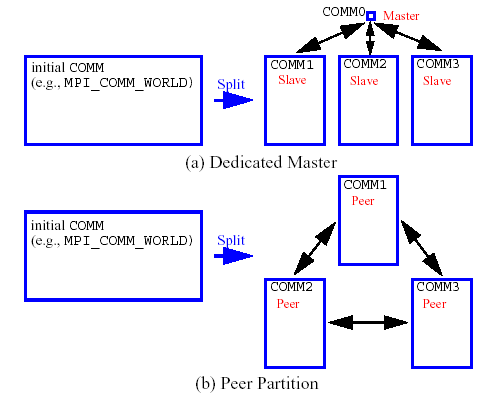
\includegraphics[width=70mm]{images/comm_partitioning}
  \caption{Communicator partitioning models.}
  \label{parallel:figure01}
\end{figure}

\subsubsection{Scheduling}\label{parallel:SLP:message:sched}

The following scheduling approaches are available within a level of
message passing parallelism:

\begin{itemize}
% TO DO: need a more descriptive term, e.g. single-point dedicated
% dynamic scheduling
\item \emph{Self-scheduling}: in the dedicated master model, the master
  processor manages a single processing queue and maintains a
  prescribed number of jobs (usually one) active on each slave. Once a
  slave server has completed a job and returned its results, the
  master assigns the next job to this slave. Thus, the slaves
  themselves determine the schedule through their job completion
  speed. This provides a simple dynamic scheduler in that
  heterogeneous processor speeds and/or job durations are naturally
  handled, provided there are sufficient instances scheduled through
  the servers to balance the variation.

\item \emph{Static scheduling}: if scheduling is statically determined
  at start-up, then no master processor is needed to direct traffic
  and a peer partitioning approach is applicable. If the static
  schedule is a good one (ideal conditions), then this approach will
  have superior performance. However, heterogeneity, when not known
  \emph{a priori}, can very quickly degrade performance since there is
  no mechanism to adapt.
\end{itemize}

%In addition, the following scheduling approach is provided by PICO for
%the scheduling of concurrent optimizations within the branch and bound
%strategy:

%\begin{itemize}
% TO DO: this could become multipoint nondedicated dynamic scheduling
%\item \emph{Distributed scheduling}: in this approach, a peer
%  partition is used and each peer maintains a separate queue of
%  pending jobs. When one peer's queue is smaller than the other
%  queues, it requests work from its peers (prior to idleness). In this
%  way, it can adapt to heterogeneous conditions, provided there are
%  sufficient instances to balance the variation. Each partition
%  performs communication between computations, and no processors are
%  dedicated to scheduling. Furthermore, it distributes scheduling load
%  beyond a single processor, which can be important for large numbers
%  of concurrent jobs (whose scheduling might overload a single master)
%  or for fault tolerance (avoiding a single point of failure).
%  However, it involves relatively complicated logic and additional
%  communication for queue status and job migration, and its
%  performance is not always superior since a partition can become
%  work-starved if its peers are locked in computation (Note: this
%  logic can be somewhat simplified if a separate thread can be created
%  for communication and migration of jobs).
%\end{itemize}

Message passing schedulers may be used for managing concurrent
iterator executions within a strategy, concurrent evaluations within
an iterator, or concurrent analyses within an evaluation.  In each of
these cases, the message passing scheduler is currently restricted to
blocking synchronization, in that all jobs in the queue are completed
before exiting the scheduler and returning the set of results to the
algorithm. Nonblocking message-passing schedulers are under
development for the iterator/evaluation concurrency level in support
of fully asynchronous algorithms which do not contain synchronization
points (e.g., \texttt{asynch\_pattern\_search} and
\texttt{coliny\_pattern\_search}).  Message passing is also used within
a fine-grained parallel analysis code, although this does not involve
the use of DAKOTA schedulers (DAKOTA may, at most, pass a communicator
partition to the simulation).  The ``Message Passing'' column in
Table~\ref{parallel:table01} summarizes these capabilities.

\subsubsection{Message Passing Example}\label{parallel:SLP:message:ex}

Revisiting the test file \texttt{dakota\_dace.in}, DAKOTA will now
compute the 49 orthogonal array samples using a message passing
approach.  In this case, a parallel launch utility is used to execute
DAKOTA across multiple processors using syntax similar to the following:
\begin{small}
\begin{verbatim}
    mpirun -np 5 -machinefile machines dakota -i dakota_dace.in
\end{verbatim}
\end{small}

Since the asynchronous local parallelism will not be used, the
interface specification does not include the \texttt{asynchronous}
keyword and would appear similar to:
\begin{small}
\begin{verbatim}
    interface,
            system
              analysis_driver = 'text_book'
\end{verbatim}
\end{small}

The relevant excerpts from the DAKOTA output for a dedicated master
partition and self-schedule, the default when the maximum concurrency
(49) exceeds the available capacity (5), would appear similar to the
following:
\begin{small}
\begin{verbatim}
    Running MPI executable in parallel on 5 processors.

    -----------------------------------------------------------------------------
    DAKOTA parallel configuration:

    Level                   num_servers    procs_per_server    partition/schedule
    -----                   -----------    ----------------    ------------------
    concurrent iterators         1                5              peer/static
    concurrent evaluations       4                1              ded. master/self
    concurrent analyses          1                1              peer/static
    multiprocessor analysis      1               N/A                N/A

    Total parallelism levels =   1
    -----------------------------------------------------------------------------

    >>>>> Running dace iterator.

    ------------------------------
    Begin Function Evaluation    1
    ------------------------------
    (Asynchronous job 1 added to queue)

    ------------------------------
    Begin Function Evaluation    2
    ------------------------------
    (Asynchronous job 2 added to queue)

    <snip>

    ------------------------------
    Begin Function Evaluation   49
    ------------------------------
    (Asynchronous job 49 added to queue)

    Blocking synchronize of 49 asynchronous evaluations
    First pass: assigning 4 jobs among 4 servers
    Master assigning function evaluation 1 to server 1
    Master assigning function evaluation 2 to server 2
    Master assigning function evaluation 3 to server 3
    Master assigning function evaluation 4 to server 4
    Second pass: self-scheduling 45 remaining jobs
    Waiting on completed jobs
    job 1 has returned from slave server 1
    Master assigning function evaluation 5 to server 1
    job 2 has returned from slave server 2
    Master assigning function evaluation 6 to server 2
    Waiting on completed jobs
    job 3 has returned from slave server 3
    Master assigning function evaluation 7 to server 3
    job 4 has returned from slave server 4
    Master assigning function evaluation 8 to server 4

    <snip>

    job 49 has returned from slave server 2

    <<<<< Iterator dace completed.
\end{verbatim}
\end{small}
where it is evident that each of the 49 jobs is first queued and then
a blocking synchronization is performed.  This synchronization uses a
dynamic scheduler that initiates four jobs by sending a message from
the master to each of the four servers and then replaces completing
jobs with new ones until all 49 are complete.  It is important to note
that job execution local to each of the four servers is synchronous.


\subsection{Hybrid Parallelism}\label{parallel:SLP:hybrid}

The asynchronous local approaches described in
Section~\ref{parallel:SLP:local} can be considered to rely on
\emph{external} scheduling mechanisms, since it is generally the
operating system or some external queue/load sharing software that
allocates jobs to processors. Conversely, the message-passing
approaches described in Section~\ref{parallel:SLP:message} rely on
\emph{internal} scheduling mechanisms to distribute work among
processors. These two approaches provide building blocks which can be
combined in a variety of ways to manage parallelism at multiple
levels. At one extreme, DAKOTA can execute on a single processor and
rely completely on external means to map all jobs to processors (i.e.,
using asynchronous local approaches). At the other extreme, DAKOTA can
execute on many processors and manage all levels of parallelism,
including the parallel simulations, using completely internal
approaches (i.e., using message passing at all levels as in
Figure~\ref{parallel:figure02}). While all-internal or all-external
approaches are common cases, many additional approaches exist between
the two extremes in which some parallelism is managed internally and
some is managed externally.

These combined approaches are referred to as \emph{hybrid}
parallelism, since the internal distribution of work based on
message-passing is being combined with external allocation using
asynchronous local approaches\footnote{The term ``hybrid parallelism''
is often used to describe the combination of MPI message passing and
OpenMP shared memory parallelism models.  This can be considered to be
a special case of the meaning here, as OpenMP is based on threads,
which is analagous to asynchronous local usage of the direct
simulation interface.}.  Figure~\ref{parallel:figure03} depicts the
asynchronous local, message-passing, and hybrid approaches for a
dedicated-master partition. Approaches (b) and (c) both use MPI
message-passing to distribute work from the master to the slaves, and
approaches (a) and (c) both manage asynchronous jobs local to a
processor. The hybrid approach (c) can be seen to be a combination of
(a) and (b) since jobs are being internally distributed to slave
servers through message-passing and each slave server is managing
multiple concurrent jobs using an asynchronous local approach. From a
different perspective, one could consider (a) and (b) to be special
cases within the range of configurations supported by (c). The hybrid
approach is useful for supercomputers that maintain a service/compute
node distinction and for supercomputers or networks of workstations
that involve clusters of symmetric multiprocessors (SMPs). In the
service/compute node case, concurrent multiprocessor simulations are
launched into the compute nodes from the service node partition. While
an asynchronous local approach from a single service node would be
sufficient, spreading the application load by running DAKOTA in
parallel across multiple service nodes results in better
performance~\cite{Eld00}. If the number of concurrent jobs to be
managed in the compute partition exceeds the number of available
service nodes, then hybrid parallelism is the preferred approach. In
the case of a cluster of SMPs (or network of multiprocessor
workstations), message-passing can be used to communicate between
SMPs, and asynchronous local approaches can be used within an
SMP. Hybrid parallelism can again result in improved performance,
since the total number of DAKOTA MPI processes is reduced in
comparison to a pure message-passing approach over all processors.

Hybrid schedulers may be used for managing concurrent evaluations
within an iterator or concurrent analyses within an evaluation.  In
both of these cases, the scheduler is currently restricted to blocking
synchronization, although as for message-passing schedulers described
in Section~\ref{parallel:SLP:message:sched}, nonblocking schedulers
are under development for the iterator/evaluation concurrency level.
The ``Hybrid'' column in Table~\ref{parallel:table01} summarizes these
capabilities.

\subsubsection{Hybrid Example}\label{parallel:SLP:hybrid:ex}

Revisiting the test file \texttt{dakota\_dace.in}, DAKOTA will now
compute the 49 orthogonal array samples using a hybrid approach.  As
for the message passing case, a parallel launch utility is used to
execute DAKOTA across multiple processors:
\begin{small}
\begin{verbatim}
    mpirun -np 5 -machinefile machines dakota -i dakota_dace.in
\end{verbatim}
\end{small}

Since the asynchronous local parallelism will also be used, the
interface specification includes the \texttt{asynchronous}
keyword and appears similar to
\begin{small}
\begin{verbatim}
    interface,
            system asynchronous evaluation_concurrency = 2
              analysis_driver = 'text_book'
\end{verbatim}
\end{small}
In the hybrid case, the specification of the desired concurrency level
must be included, since the default is no longer all available (as it
is for asynchronous local parallelism).  Rather the default is to employ
message passing parallelism, and hybrid parallelism is only available
through the specification of asynchronous concurrency greater than one.

The relevant excerpts of the DAKOTA output for a dedicated master
partition and self schedule, the default when the maximum concurrency
(49) exceeds the maximum available capacity (10), would appear similar
to the following:
\begin{small}
\begin{verbatim}
    Running MPI executable in parallel on 5 processors.

    -----------------------------------------------------------------------------
    DAKOTA parallel configuration:

    Level                   num_servers    procs_per_server    partition/schedule
    -----                   -----------    ----------------    ------------------
    concurrent iterators         1                5              peer/static
    concurrent evaluations       4                1              ded. master/self
    concurrent analyses          1                1              peer/static
    multiprocessor analysis      1               N/A                N/A

    Total parallelism levels =   1
    -----------------------------------------------------------------------------

    >>>>> Running dace iterator.

    ------------------------------
    Begin Function Evaluation    1
    ------------------------------
    (Asynchronous job 1 added to queue)

    ------------------------------
    Begin Function Evaluation    2
    ------------------------------
    (Asynchronous job 2 added to queue)

    <snip>

    ------------------------------
    Begin Function Evaluation   49
    ------------------------------
    (Asynchronous job 49 added to queue)

    Blocking synchronize of 49 asynchronous evaluations
    First pass: assigning 8 jobs among 4 servers
    Master assigning function evaluation 1 to server 1
    Master assigning function evaluation 2 to server 2
    Master assigning function evaluation 3 to server 3
    Master assigning function evaluation 4 to server 4
    Master assigning function evaluation 5 to server 1
    Master assigning function evaluation 6 to server 2
    Master assigning function evaluation 7 to server 3
    Master assigning function evaluation 8 to server 4
    Second pass: self-scheduling 41 remaining jobs
    Waiting on completed jobs

    <snip>

    job 49 has returned from slave server 4

    <<<<< Iterator dace completed.
\end{verbatim}
\end{small}
where it is evident that each of the 49 jobs is first queued and then
a blocking synchronization is performed.  This synchronization uses a
dynamic scheduler that initiates eight jobs by sending two messages to
each of the four servers and then replaces completing jobs with new
ones until all 49 are complete.  It is important to note that job
execution local to each of the four servers is asynchronous.  If the
available capacity was increased to meet or exceed the maximum
concurrency (e.g., mpirun on 10 processors with
\texttt{evaluation\_concurrency = 5}), then a peer partition with
static schedule would be selected by default.


\section{Multilevel parallelism} \label{parallel:MLP}


Parallel computers within the Department of Energy national
laboratories have exceeded a hundred trillion floating point
operations per second (100 TeraFLOPS) in Linpack benchmarks and are
expected to achieve PetaFLOPS speeds in the near future. This
performance is achieved through the use of massively parallel (MP)
processing using $O[10^{3}-10^{4}]$ processors. In order to harness
the power of these machines for performing design, uncertainty
quantification, and other systems analyses, parallel algorithms are
needed which are scalable to thousands of processors.

DAKOTA supports a total of three tiers of scheduling and four levels
of parallelism which, in combination, can minimize efficiency losses
and achieve near linear scaling on MP computers. The four levels are:
\begin{enumerate}
\item concurrent iterators within a strategy (scheduling performed by
  DAKOTA)

\item concurrent function evaluations within each iterator (scheduling
  performed by DAKOTA)

\item concurrent analyses within each function evaluation (scheduling
  performed by DAKOTA)

\item multiprocessor analyses (work distributed by a parallel
  analysis code)
\end{enumerate}
for which the first two are classified as algorithmic coarse-grained
parallelism, the third is function evaluation coarse-grained
parallelism, and the fourth is function evaluation fine-grained
parallelism (see Section~\ref{parallel:overview:cat}). Algorithmic
fine-grained parallelism is not currently supported, although the
development of large-scale parallel SAND techniques is a current
research direction~\cite{Bar01b}.

A particular application may support one or more of these parallelism
types, and DAKOTA provides for convenient selection and combination of
each of the supported levels. If multiple types of parallelism can be
exploited, then the question may arise as to how the amount of
parallelism at each level should be selected so as to maximize the
overall parallel efficiency of the study. For performance analysis of
multilevel parallelism formulations and detailed discussion of these
issues, refer to~\cite{Eld00}.  In many cases, \emph{the user may
simply employ DAKOTA's automatic parallelism configuration facilities,}
which implement the recommendations from the aforementioned paper.

Figure~\ref{fig:mlp_scaling} shows typical fixed-size scaling
performance using a modified version of the extended
\texttt{text\_book} problem (see Section~\ref{additional:textbook}).
Three levels of parallelism (concurrent evaluations within an
iterator, concurrent analyses within each evaluation, and
multiprocessor analyses) are exercised.  Despite the use of a fixed
problem size and the presence of some idleness within the scheduling
at multiple levels, the efficiency is still reasonably
high\footnote{Note that overhead is reduced in these scaling studies
by deactivating the evaluation cache and restart file logging.}.
Greater efficiencies are obtainable for scaled speedup studies (or for
larger problems in fixed-size studies) and for problems optimized for
minimal scheduler idleness (by, e.g., managing all concurrency in as
few scheduling levels as possible).  Note that speedup and efficiency
are measured relative to the case of a single instance of a
multiprocessor analysis, since it was desired to investigate the
effectiveness of the DAKOTA schedulers independent from the efficiency
of the parallel analysis.
\begin{figure}[ht]
  \centering
  \subfigure[Relative speedup.]
    {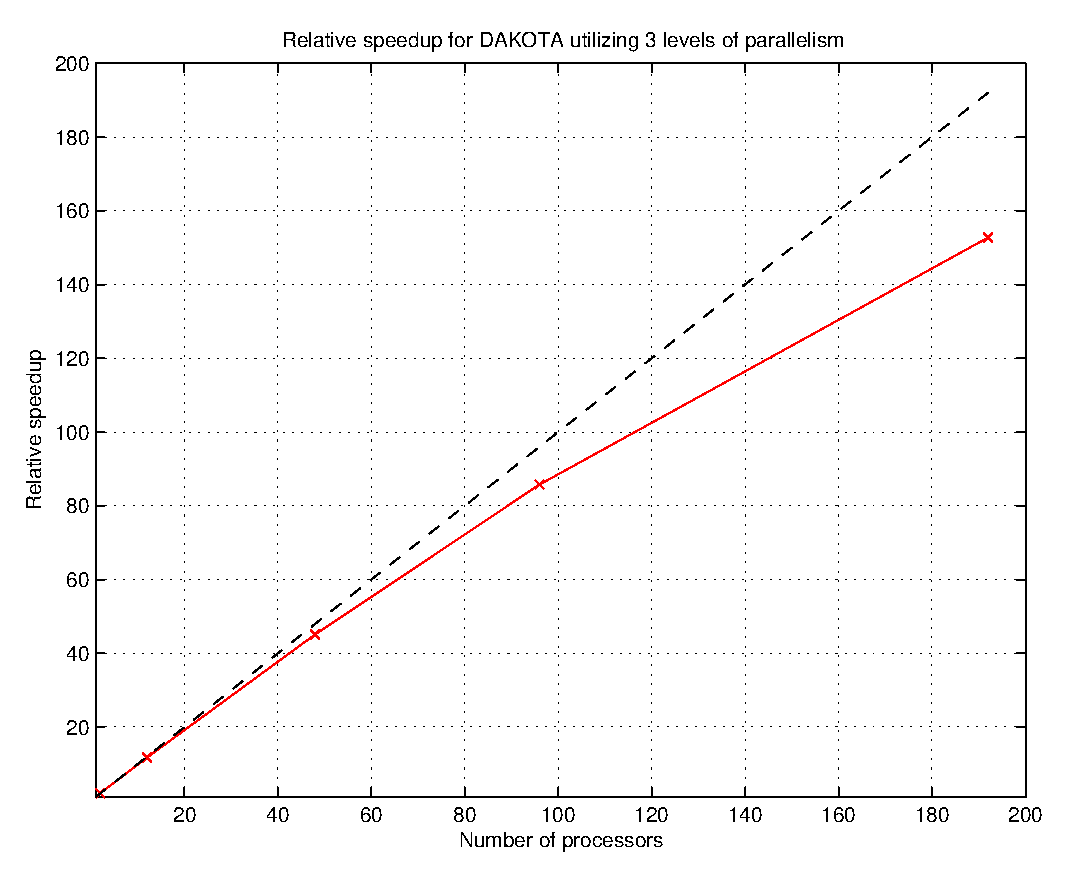
\includegraphics[width=.45\textwidth]{images/mss_rel_speedup_3lev_determ}}
  \subfigure[Relative efficiency.]
    {\includegraphics[width=.45\textwidth]{images/mss_rel_eff_3lev_determ}}
  \caption{Fixed-size scaling results for three levels of parallelism.}
  \label{fig:mlp_scaling}
% The 2 processor run uses a 1/1/1/2 configuration and is as small as can be
% fairly compared for the same level of fine-grained simulation.  The 12, 48,
% 96, and 192 processor runs use 3 levels of parallelism in a 1/eval_srv/3/2
% configuration with eval_srv = 2, 8, 16, and 32, respectively.
\end{figure}

\subsection{Asynchronous Local Parallelism}\label{parallel:MLP:local}

In most cases, the use of asynchronous local parallelism is the
termination point for multilevel parallelism, in that any level of
parallelism lower than an asynchronous local level will be serialized.
The exception to this rule is reforking of forked processes for
concurrent analyses within forked evaluations.  In this case, a new
process is created using fork for one of several concurrent
evaluations; however, the new process is not replaced immediately
using exec.  Rather, the new process is reforked to create additional
child processes for executing concurrent analyses within each
concurrent evaluation process.  This capability is not supported by
system calls and provides one of the key advantages to using fork over
system (see Section~\ref{interfaces:which}).

\subsection{Message Passing Parallelism}\label{parallel:MLP:message}

%\subsection{Communicator partitioning}
%   Lowest level supports single-level options above
\subsubsection{Partitioning of levels}\label{parallel:MLP:message:partitioning}

DAKOTA uses MPI communicators to identify groups of processors. The
global \texttt{MPI\_COMM\_WORLD} communicator provides the total set
of processors allocated to the DAKOTA run. \texttt{MPI\_COMM\_WORLD}
can be partitioned into new intra-communicators which each define a
set of processors to be used for a multiprocessor server. Each of
these servers may be further partitioned to nest one level of
parallelism within the next. At the lowest parallelism level, these
intra-communicators can be passed into a simulation for use as the
simulation's computational context, provided that the simulation has
been designed, or can be modified, to be modular on a communicator
(i.e., it does not assume ownership of \texttt{MPI\_COMM\_WORLD}). New
intra-communicators are created with the \texttt{MPI\_Comm\_split}
routine, and in order to send messages between these
intra-communicators, new inter-communicators are created with calls to
\texttt{MPI\_Intercomm\_create}. To minimize overhead, DAKOTA creates
new intra- and inter-communicators only when the parent communicator
provides insufficient context for the scheduling at a particular
level. In addition, multiple parallel configurations (containing a set
of communicator partitions) can be allocated for use in studies with
multiple iterators and models (e.g., 16 servers of 64 processors each
could be used for iteration on a lower fidelity model, followed by two
servers of 512 processors each for subsequent iteration on a higher
fidelity model).  Each of the parallel configurations are allocated
at object construction time and are reported at the beginning of the
DAKOTA output.

Each tier within DAKOTA's nested parallelism hierarchy can use the
dedicated master and peer partition approaches described in
Section~\ref{parallel:SLP:message:part}. To recursively partition the
subcommunicators of Figure~\ref{parallel:figure01},
\texttt{COMM1/2/3} in the dedicated master or peer partition case
would be further subdivided using the appropriate partitioning model
for the next lower level of parallelism.


\subsubsection{Scheduling within levels}\label{parallel:MLP:message:scheduling}

\begin{figure}[ht]
  \centering
  \includegraphics[width=60mm]{images/recursive_partitioning}
  \caption{Recursive partitioning for nested parallelism.}
  \label{parallel:figure02}
\end{figure}

DAKOTA is designed to allow the freedom to configure each parallelism
level with either the dedicated master partition/self-scheduling
combination or the peer partition/static scheduling combination. In
addition, certain external libraries may provide additional options.
%(e.g., PICO supports distributed scheduling in peer partitions).
As an
example, Figure~\ref{parallel:figure02} shows a case in which a branch
and bound strategy employs peer partition/distributed scheduling at
level 1, each optimizer partition employs concurrent function
evaluations in a dedicated master partition/self-scheduling model at
level 2, and each function evaluation partition employs concurrent
multiprocessor analyses in a peer partition/static scheduling model at
level 3. In this case, \texttt{MPI\_COMM\_WORLD} is subdivided into
\texttt{optCOMM1/2/3/.../$\tau_{1}$}, each \texttt{optCOMM} is further
subdivided into \texttt{evalCOMM0} (master) and
\texttt{evalCOMM1/2/3/.../$\tau_{2}$} (slaves), and each slave
\texttt{evalCOMM} is further subdivided into
\texttt{analCOMM1/2/3/.../$\tau_{3}$}.  Logic for selection of $\tau_i$
is discussed in~\cite{Eld00}.


\subsection{Hybrid Parallelism}\label{parallel:MLP:hybrid}

Hybrid parallelism approaches can take several forms when used in the
multilevel parallel context. A conceptual boundary can be considered
to exist for which all parallelism above the boundary is managed
internally using message-passing and all parallelism below the
boundary is managed externally using asynchronous local approaches.
Hybrid parallelism approaches can then be categorized based on whether
this boundary between internal and external management occurs within a
parallelism level (\emph{intra-level}) or between two parallelism
levels (\emph{inter-level}). In the intra-level case, the jobs for the
parallelism level containing the boundary are scheduled using a hybrid
scheduler, in which a capacity multiplier is used for the number of
jobs to assign to each server. Each server is then responsible for
concurrently executing its capacity of jobs using an asynchronous
local approach. In the inter-level case, one level of parallelism
manages its parallelism internally using a message-passing approach
and the next lower level of parallelism manages its parallelism
externally using an asynchronous local approach. That is, the jobs for
the higher level of parallelism are scheduled using a standard
message-passing scheduler, in which a single job is assigned to each
server. However, each of these jobs has multiple components, as
managed by the next lower level of parallelism, and each server is
responsible for executing these sub-components concurrently using an
asynchronous local approach.

For example, consider a multiprocessor DAKOTA run which involves an
iterator scheduling a set of concurrent function evaluations across a
cluster of SMPs. A hybrid parallelism approach will be applied in
which message-passing parallelism is used between SMPs and
asynchronous local parallelism is used within each SMP. In the hybrid
intra-level case, multiple function evaluations would be scheduled to
each SMP, as dictated by the capacity of the SMPs, and each SMP would
manage its own set of concurrent function evaluations using an
asynchronous local approach. Any lower levels of parallelism would be
serialized. In the hybrid inter-level case, the function evaluations
would be scheduled one per SMP, and the analysis components within
each of these evaluations would be executed concurrently using
asynchronous local approaches within the SMP. Thus, the distinction
can be viewed as whether the concurrent jobs on each server in
Figure~\ref{parallel:figure03}c reflect the same level of parallelism
as that being scheduled by the master (intra-level) or one level of
parallelism below that being scheduled by the master (inter-level).


\section{Capability Summary}\label{parallel:summary}


Table~\ref{parallel:table01} shows a matrix of the supported job
management approaches for each of the parallelism levels, with
supported simulation interfaces and synchronization approaches shown
in parentheses. The concurrent iterator and multiprocessor analysis
parallelism levels can only be managed with message-passing
approaches. In the former case, this is due to the fact that a
separate process or thread for an iterator is not currently supported.
The latter case reflects a finer point on the definition of external
parallelism management. While a multiprocessor analysis can most
certainly be launched (e.g., using \texttt{mpirun}/\texttt{yod}) from
one of DAKOTA's analysis drivers, resulting in a parallel analysis
external to DAKOTA (which is consistent with asynchronous local and
hybrid approaches), this parallelism is not visible to DAKOTA and
therefore does not qualify as parallelism that DAKOTA manages (and
therefore is not included in Table~\ref{parallel:table01}). The
concurrent evaluation and analysis levels can be managed either with
message-passing, asynchronous local, or hybrid techniques, with the
exceptions that the direct interface does not support asynchronous
operations (asynchronous local or hybrid) at either of these levels
and the system call interface does not support asynchronous operations
(asynchronous local or hybrid) at the concurrent analysis level. The
direct interface restrictions are present since multithreading in not
yet supported and the system call interface restrictions result from
the inability to manage concurrent analyses within a nonblocking
function evaluation system call.  Finally, nonblocking synchronization
is only currently supported for asynchronous local parallelism at the
concurrent function evaluation level.  In time, message passing and
hybrid parallelism approaches will also support nonblocking
synchronization at this level.

\begin{table}
  \centering
  \caption{Support of job management approaches within parallelism levels.
  Shown in parentheses are supported simulation interfaces and supported
  synchronization approaches.}
  \label{parallel:table01}\vspace{2mm}
  \begin{tabular}{c||c|c|c|}
    %\hline
    \textbf{Parallelism Level} & \textbf{Asynchronous Local} &
    \textbf{Message Passing} & \textbf{Hybrid} \\
    \hline \hline
    concurrent iterators & & \textbf{X}      & \\
    within a strategy    & & (blocking only) & \\
    \hline
    concurrent function evaluations & \textbf{X} & \textbf{X} & \textbf{X} \\
    within an iterator          & (system, fork) & (system, fork, direct) &
    (system, fork) \\
    & (blocking, nonblocking) & (blocking only) & (blocking only) \\
    \hline
    concurrent analyses & \textbf{X} & \textbf{X} & \textbf{X} \\
    within a function evaluation & (fork only) & (system, fork, direct) &
    (fork only) \\
    & (blocking only) & (blocking only) & (blocking only) \\
    \hline
    fine-grained parallel analysis & & \textbf{X} & \\
    \hline
  \end{tabular}
\end{table}


\section{Running a Parallel DAKOTA Job}\label{parallel:running}


Section~\ref{parallel:SLP} provides a few examples of serial and
parallel execution of DAKOTA using asynchronous local, message
passing, and hybrid approaches to single-level parallelism.  The
following sections provides a more complete discussion of the parallel
execution syntax and available specification controls.


\subsection{Single-processor execution}\label{parallel:running:single}

The command for running DAKOTA on a single-processor and exploiting
asynchronous local parallelism is the same as for running DAKOTA on a
single-processor for a serial study, e.g.:
\begin{small}
\begin{verbatim}
    dakota -i dakota.in > dakota.out
\end{verbatim}
\end{small}

See Section~\ref{tutorial:installation:running} for additional
information on single-processor command syntax.

\subsection{Multiprocessor execution}\label{parallel:running:multiprocessor}

Running a DAKOTA job on multiple processors requires the use of an
executable loading facility such as \texttt{mpirun}, \texttt{mpiexec},
\texttt{poe}, or \texttt{yod}.  On a network of workstations, the
\texttt{mpirun} script is commonly used to initiate a parallel DAKOTA
job, e.g.:
\begin{small}
\begin{verbatim}
    mpirun -np 12 dakota -i dakota.in > dakota.out
    mpirun -machinefile machines -np 12 dakota -i dakota.in > dakota.out
\end{verbatim}
\end{small}
where both examples specify the use of 12 processors, the former
selecting them from a default system resources file and the latter
specifying particular machines in a machine file (see~\cite{Gro96} for
details).

On a massively parallel computer such as ASCI Red, similar facilities
are available from the Cougar operating system via the \texttt{yod}
executable loading facility:
\begin{small}
\begin{verbatim}
    yod -sz 512 dakota -i dakota.in > dakota.out
\end{verbatim}
\end{small}

In each of these cases, MPI command line arguments are used by MPI
(extracted first in the call to \texttt{MPI\_Init}) and DAKOTA command
line arguments are used by DAKOTA (extracted second by DAKOTA's
command line handler). An issue that can arise with these command line
arguments is that the mpirun script distributed with MPICH has been
observed to have problems with certain file path specifications (e.g.,
a relative path such as ``\texttt{../some\_file}''). These path
problems are most easily resolved by using local linkage (all
referenced files or soft links to these files appear in the same
directory).

Finally, when running on computer resources that employ NQS/PBS batch
schedulers, the single-processor \texttt{dakota} command syntax or the
multiprocessor \texttt{mpirun} command syntax might be contained
within an executable script file which is submitted to the batch
queue. For example, on Cplant, the command
\begin{small}
\begin{verbatim}
    qsub -l size=512 run_dakota
\end{verbatim}
\end{small}

could be submitted to the PBS queue for execution. On ASCI Red, the
NQS syntax is similar:
\begin{small}
\begin{verbatim}
    qsub -q snl -lP 512 -lT 6:00:00 run_dakota
\end{verbatim}
\end{small}

These commands allocate 512 compute nodes for the study, and execute
the \texttt{run\_dakota} script on a service node. If this script
contains a single-processor \texttt{dakota} command, then DAKOTA will
execute on a single service node from which it can launch parallel
simulations into the compute nodes using analysis drivers that contain
\texttt{yod} commands (any \texttt{yod} executions occurring at any
level underneath the \texttt{run\_dakota} script are mapped to the 512
compute node allocation). If the script submitted to \texttt{qsub}
contains a multiprocessor \texttt{mpirun} command, then DAKOTA will
execute across multiple service nodes so that it can spread the
application load in either a message-passing or hybrid parallelism
approach. Again, analysis drivers containing \texttt{yod} commands
would be responsible for utilizing the 512 compute nodes. And,
finally, if the script submitted to \texttt{qsub} contains a
\texttt{yod} of the \texttt{dakota} executable, then DAKOTA will
execute directly on the compute nodes and manage all of the
parallelism internally (note that a \texttt{yod} of this type without
a \texttt{qsub} would be mapped to the interactive partition, rather
than to the batch partition).

Not all supercomputers employ the same model for service/compute
partitions or provide the same support for tiling of concurrent
multiprocessor simulations within a single NQS/PBS allocation.  For
this reason, templates for parallel job configuration are being
catalogued within {\tt Dakota/examples/script\_interfaces} and 
\texttt{Dakota/examples/parallelism} (in the software
distributions) that are intended to provide guidance for individual
machine idiosyncrasies.

\section{Specifying Parallelism}\label{parallel:spec}

Given an allotment of processors, DAKOTA contains logic based on the
theoretical work in~\cite{Eld00} to automatically determine an efficient
parallel configuration, consisting of partitioning and scheduling
selections for each of the parallelism levels. This logic accounts for
problem size, the concurrency supported by particular iterative
algorithms, and any user inputs or overrides. The following points are
important components of the automatic configuration logic which can be
helpful in estimating the total number of processors to allocate and
in selecting configuration overrides:

\begin{itemize}
\item If the capacity of the servers in a peer configuration is
  sufficient to schedule all jobs in one pass, then a peer partition
  and static schedule will be selected. If this capacity is not
  sufficient, then a dedicated-master partition and dynamic schedule
  will be used. These selections can be overridden with self/static
  scheduling request specifications for the concurrent iterator,
  evaluation, and analysis parallelism levels. For example, if it is
  known that processor speeds and job durations have little
  variability, then overriding the automatic configuration with a
  static schedule request could eliminate the unnecessary loss of a
  processor to scheduling.

\item With the exception of the concurrent-iterator parallelism level
  (iterator executions tend to have high variability in duration),
  concurrency is pushed up. That is, available processors will be
  assigned to concurrency at the higher parallelism levels first. If
  more processors are available than needed for concurrency at a
  level, then the server size is increased to support concurrency in
  the next lower level of parallelism. This process is continued until
  all available processors have been assigned. These assignments can
  be overridden with a servers specification for the concurrent
  iterator, evaluation, and analysis parallelism levels and with a
  processors per analysis specification for the multiprocessor
  analysis parallelism level. For example, if it is desired to
  parallelize concurrent analyses within each function evaluation,
  then an \texttt{evaluation\_servers = 1} override would serialize
  the concurrent function evaluations level and assure processor
  availability for concurrent analyses.
\end{itemize}

In the following sections, the user inputs and overrides are
described, followed by specification examples for single and
multi-processor DAKOTA executions.

\subsection{The interface specification}\label{parallel:spec:interface}

Specifying parallelism within an interface can involve the use of the
\texttt{asynchronous}, \texttt{evaluation\_concurrency}, and
\texttt{analysis\_concurrency} keywords to specify concurrency local
to a processor (i.e., asynchronous local parallelism). This
\texttt{asynchronous} specification has dual uses:

\begin{itemize}
\item When running DAKOTA on a single-processor, the
  \texttt{asynchronous} keyword specifies the use of asynchronous
  invocations local to the processor (these jobs then rely on external
  means to be allocated to other processors). The default behavior is
  to simultaneously launch all function evaluations available from the
  iterator as well as all available analyses within each function
  evaluation. In some cases, the default behavior can overload a
  machine or violate a usage policy, resulting in the need to limit
  the number of concurrent jobs using the
  \texttt{evaluation\_concurrency} and \texttt{analysis\_concurrency}
  specifications.

\item When executing DAKOTA across multiple processors and managing
  jobs with a message-passing scheduler, the \texttt{asynchronous}
  keyword specifies the use of asynchronous invocations local to each
  server processor, resulting in a hybrid parallelism approach (see
  Section~\ref{parallel:SLP:hybrid}). In this case, the default
  behavior is one job per server, which must be overridden with an
  \texttt{evaluation\_concurrency} specification and/or an
  \texttt{analysis\_concurrency} specification. When a hybrid
  parallelism approach is specified, the capacity of the servers (used
  in the automatic configuration logic) is defined as the number of
  servers times the number of asynchronous jobs per server.
\end{itemize}

In addition, \texttt{evaluation\_servers},
\texttt{evaluation\_self\_scheduling}, and
\texttt{evaluation\_static\_scheduling} keywords can be used to
override the automatic parallelism configuration for concurrent
function evaluations; \texttt{analysis\_servers},
\texttt{analysis\_self\_scheduling}, and
\texttt{analysis\_static\_scheduling} keywords can be used to override
the automatic parallelism configuration for concurrent analyses; and
the \texttt{processors\_per\_analysis} keyword can be used to override
the automatic parallelism configuration for the size of multiprocessor
analyses used in a direct function simulation interface. Each of these
keywords appears as part of the interface commands specification in
the DAKOTA Reference Manual~\cite{RefMan}.

\subsection{The strategy specification}\label{parallel:spec:strategy}

To specify concurrency in iterator executions, the
\texttt{iterator\_servers}, \texttt{iterator\_self\_scheduling}, and
\texttt{iterator\_static\_scheduling} keywords are used to override
the automatic parallelism configuration. See the strategy commands
specification in the DAKOTA Reference Manual~\cite{RefMan} for additional
information.

\subsection{Single-processor DAKOTA specification}\label{parallel:spec:single}

Specifying a single-processor DAKOTA job that exploits parallelism
through asynchronous local approaches (see
Figure~\ref{parallel:figure03}a) requires inclusion of the
\texttt{asynchronous} keyword in the interface specification. Once the
input file is defined, single-processor DAKOTA jobs are executed using
the command syntax described previously in
Section~\ref{parallel:running:single}.

\subsubsection{Example 1}\label{parallel:spec:single:example1}

For example, the following specification runs an NPSOL optimization
which will perform asynchronous finite differencing:
\begin{small}
\begin{verbatim}
    method,
            npsol_sqp

    variables,
            continuous_design = 5
              initial_point  0.2  0.05 0.08 0.2  0.2
              lower_bounds   0.15 0.02 0.05 0.1  0.1
              upper_bounds   2.0  2.0  2.0  2.0  2.0

    interface,
            system,
              asynchronous
              analysis_drivers = 'text_book'

    responses,
            num_objective_functions = 1
            num_nonlinear_inequality_constraints = 2
            numerical_gradients
              interval_type central
              method_source dakota
              fd_gradient_step_size = 1.e-4
            no_hessians
\end{verbatim}
\end{small}

Note that \texttt{method\_source} \texttt{dakota} selects DAKOTA's
internal finite differencing routine so that the concurrency in finite
difference offsets can be exploited. In this case, central
differencing has been selected and 11 function evaluations (one at the
current point plus two offsets in each of five variables) can be
performed simultaneously for each NPSOL response request. These 11
evaluations will be launched with system calls in the background and
presumably assigned to additional processors through the operating
system of a multiprocessor compute server or other comparable method.
The concurrency specification may be included if it is necessary to
limit the maximum number of simultaneous evaluations. For example, if
a maximum of six compute processors were available, the command
\begin{small}
\begin{verbatim}
    evaluation_concurrency = 6
\end{verbatim}
\end{small}
could be added to the \texttt{asynchronous} specification within the
\texttt{interface} keyword from the preceding example.

\subsubsection{Example 2}\label{parallel:spec:single:example2}

If, in addition, multiple analyses can be executed concurrently within
a function evaluation (e.g., from multiple load cases or disciplinary
analyses that must be evaluated to compute the response data set),
then an input specification similar to the following could be used:
\begin{small}
\begin{verbatim}
    method,
            npsol_sqp

    variables,
            continuous_design = 5
              initial_point  0.2  0.05 0.08 0.2  0.2
              lower_bounds   0.15 0.02 0.05 0.1  0.1
              upper_bounds   2.0  2.0  2.0  2.0  2.0

    interface,
            fork
              asynchronous
                evaluation_concurrency = 6
                analysis_concurrency = 3
              analysis_drivers = 'text_book1' 'text_book2' 'text_book3'

    responses,
            num_objective_functions = 1
            num_nonlinear_inequality_constraints = 2
            numerical_gradients
              method_source dakota
              interval_type central
              fd_gradient_step_size = 1.e-4
            no_hessians
\end{verbatim}
\end{small}

In this case, the default concurrency with just an
\texttt{asynchronous} specification would be all 11 function
evaluations and all 3 analyses, which can be limited by the
\texttt{evaluation\_concurrency} and \texttt{analysis\_concurrency}
specifications. The input file above limits the function evaluation
concurrency, but not the analysis concurrency (a specification of 3 is
the default in this case and could be omitted). Changing the input to
\texttt{evaluation\_concurrency = 1} would serialize the function
evaluations, and changing the input to \texttt{analysis\_concurrency = 1}
would serialize the analyses.

\subsection{Multiprocessor DAKOTA specification}\label{parallel:spec:multi}

In multiprocessor executions, server evaluations are synchronous
(Figure~\ref{parallel:figure03}b) by default and the
\texttt{asynchronous} keyword is only used if a hybrid parallelism
approach (Figure~\ref{parallel:figure03}c) is desired. Multiprocessor
DAKOTA jobs are executed using the command syntax described previously
in Section~\ref{parallel:running:multiprocessor}.

\subsubsection{Example 3}\label{parallel:spec:multi:example3}

To run Example 1 using a message-passing approach, the
\texttt{asynchronous} keyword would be removed (since the servers will
execute their evaluations synchronously), resulting in the following
interface specification:
\begin{small}
\begin{verbatim}
    interface,
            system,
              analysis_drivers = 'text_book'
\end{verbatim}
\end{small}

Running DAKOTA on 4 processors (syntax: \texttt{mpirun -np 4 dakota -i
  dakota.in}) would result in the following parallel configuration
report from the DAKOTA output:
\begin{small}
\begin{verbatim}
    -----------------------------------------------------------------------------
    DAKOTA parallel configuration:

    Level                   num_servers    procs_per_server    partition/schedule
    -----                   -----------    ----------------    ------------------
    concurrent iterators         1                4              peer/static
    concurrent evaluations       3                1              ded. master/self
    concurrent analyses          1                1              peer/static
    multiprocessor analysis      1               N/A                N/A

    Total parallelism levels =   1
    -----------------------------------------------------------------------------
\end{verbatim}
\end{small}

The dedicated master partition and self-scheduling algorithm are
automatically selected for the concurrent evaluations parallelism
level since the number of function evaluations (11) is greater than
the maximum capacity of the servers (4). Since one of the processors
is dedicated to being the master, only 3 processors are available for
computation and the 11 evaluations can be completed in approximately 4
passes through the servers. If it is known that there is little
variability in evaluation duration, then this logic could be
overridden to use a static schedule through use of the
\texttt{evaluation\_static\_scheduling} specification:
\begin{small}
\begin{verbatim}
    interface,
            system,
              evaluation_static_scheduling
              analysis_drivers = 'text_book'
\end{verbatim}
\end{small}

Running DAKOTA again on 4 processors (syntax: \texttt{mpirun -np 4
  dakota -i dakota.in}) would now result in this parallel
configuration report:
\begin{small}
\begin{verbatim}
    -----------------------------------------------------------------------------
    DAKOTA parallel configuration:

    Level                   num_servers    procs_per_server    partition/schedule
    -----                   -----------    ----------------    ------------------
    concurrent iterators         1                4              peer/static
    concurrent evaluations       4                1              peer/static
    concurrent analyses          1                1              peer/static
    multiprocessor analysis      1               N/A                N/A

    Total parallelism levels =   1
    -----------------------------------------------------------------------------
\end{verbatim}
\end{small}

Now the 11 jobs will be statically distributed among 4 peer servers,
since the processor previously dedicated to scheduling has been
converted to a compute server. This could be more efficient if the
evaluation durations are sufficiently similar, but there is no
mechanism to adapt to heterogeneity in processor speeds or simulation
expense.

As a related example, consider the case where each of the workstations
used in the parallel execution has multiple processors. In this case,
a hybrid parallelism approach which combines message-passing
parallelism with asynchronous local parallelism (see
Figure~\ref{parallel:figure03}c) would be a good choice. To specify
hybrid parallelism, one uses the same \texttt{asynchronous}
specification as was used for the single-processor examples, e.g.:
\begin{small}
\begin{verbatim}
    interface,
             system
               asynchronous evaluation_concurrency = 3
               analysis_drivers = `text_book'
\end{verbatim}
\end{small}

With 3 function evaluations concurrent on each server, the capacity of
a 4 processor DAKOTA execution (syntax: \texttt{mpirun -np 4 dakota -i
  dakota.in}) has increased to 12 evaluations. Since all 11 jobs can
now be scheduled in a single pass, a static schedule is automatically
selected (without any override request):
\begin{small}
\begin{verbatim}
    -----------------------------------------------------------------------------
    DAKOTA parallel configuration:

    Level                   num_servers    procs_per_server    partition/schedule
    -----                   -----------    ----------------    ------------------
    concurrent iterators         1                4              peer/static
    concurrent evaluations       4                1              peer/static
    concurrent analyses          1                1              peer/static
    multiprocessor analysis      1               N/A                N/A

    Total parallelism levels =   1
    -----------------------------------------------------------------------------
\end{verbatim}
\end{small}

\subsubsection{Example 4}\label{parallel:spec:multi:example4}

To run Example 2 using a message-passing approach, the
\texttt{asynchronous} specification is again removed:
\begin{small}
\begin{verbatim}
    interface,
             fork
               analysis_drivers = `text_book1' `text_book2' `text_book3'
\end{verbatim}
\end{small}

Running this example on 6 processors (syntax: \texttt{mpirun -np 6
  dakota -i dakota.in}) would result in the following parallel
configuration report:
\begin{small}
\begin{verbatim}
    -----------------------------------------------------------------------------
    DAKOTA parallel configuration:

    Level                   num_servers    procs_per_server    partition/schedule
    -----                   -----------    ----------------    ------------------
    concurrent iterators         1                6              peer/static
    concurrent evaluations       5                1              ded. master/self
    concurrent analyses          1                1              peer/static
    multiprocessor analysis      1               N/A                N/A

    Total parallelism levels =   1
    -----------------------------------------------------------------------------
\end{verbatim}
\end{small}

in which all of the processors have been assigned to support
evaluation concurrency due to the ``push up'' automatic configuration
logic. Note that the default configuration could be a poor choice in
this case, since 11 jobs scheduled through 5 servers will likely have
significant idleness towards the end of the scheduling.  To assign
some of the available processors to the concurrent analysis level, the
following input could be used:
\begin{small}
\begin{verbatim}
    interface,
             fork
               analysis_drivers = `text_book1' `text_book2' `text_book3'
               evaluation_static_scheduling
               evaluation_servers = 2
\end{verbatim}
\end{small}

which results in the following 2-level parallel configuration:
\begin{small}
\begin{verbatim}
    -----------------------------------------------------------------------------
    DAKOTA parallel configuration:

    Level                   num_servers    procs_per_server    partition/schedule
    -----                   -----------    ----------------    ------------------
    concurrent iterators         1                6              peer/static
    concurrent evaluations       2                3              peer/static
    concurrent analyses          3                1              peer/static
    multiprocessor analysis      1               N/A                N/A

    Total parallelism levels =   2
    -----------------------------------------------------------------------------
\end{verbatim}
\end{small}

The six processors available have been split into two evaluation
servers of three processors each, where the three processors in each
evaluation server manage the three analyses, one per processor.

Next, consider the following 3-level parallel case, in which
\texttt{text\_book1}, \texttt{text\_book2}, and \texttt{text\_book3}
from the previous examples now execute on two processors each. In this
case, the \texttt{processors\_per\_analysis} keyword is added and the
\texttt{fork} interface is changed to a \texttt{direct} interface
since the fine-grained parallelism of the three simulations is managed
internally:
\begin{small}
\begin{verbatim}
    interface,
             direct
               analysis_drivers = `text_book1' `text_book2' `text_book3'
               evaluation_static_scheduling
               evaluation_servers = 2
               processors_per_analysis = 2
\end{verbatim}
\end{small}

This results in the following parallel configuration for a 12
processor DAKOTA run \\
(syntax: \texttt{mpirun -np 12 dakota -i dakota.in}):
\begin{small}
\begin{verbatim}
    -----------------------------------------------------------------------------
    DAKOTA parallel configuration:

    Level                   num_servers    procs_per_server    partition/schedule
    -----                   -----------    ----------------    ------------------
    concurrent iterators         1               12              peer/static
    concurrent evaluations       2                6              peer/static
    concurrent analyses          3                2              peer/static
    multiprocessor analysis      2               N/A                N/A

    Total parallelism levels =   3
    -----------------------------------------------------------------------------
\end{verbatim}
\end{small}

An important point to recognize is that, since each of the parallel
configuration inputs has been tied to the interface specification up
to this point, these parallel configurations can be reallocated for
each interface in a multi-iterator/multi-model strategy. For example,
a DAKOTA execution on 40 processors might involve the following two
interface specifications:
\begin{small}
\begin{verbatim}
    interface,
            direct,
              id_interface = 'COARSE'
              analysis_driver = 'sim1'
              processors_per_analysis = 5

    interface,
            direct,
              id_interface = 'FINE'
              analysis_driver = 'sim2'
              processors_per_analysis = 10
\end{verbatim}
\end{small}

for which the coarse model would employ 8 servers of 5 processors each
and the fine model would employ 4 servers of 10 processors each.

Next, consider the following 4-level parallel case that employs the
Pareto set optimization strategy. In this case,
\texttt{iterator\_servers} and \texttt{iterator\_static\_scheduling}
requests are included in the strategy specification:
\begin{small}
\begin{verbatim}
    strategy,
             pareto_set
               iterator_servers = 2
               iterator_static_scheduling
               opt_method_pointer = 'NLP'
               random_weight_sets = 4
\end{verbatim}
\end{small}

Adding this strategy specification to the input file from the previous
12 processor example results in the following parallel configuration
for a 24 processor DAKOTA run \\
(syntax: \texttt{mpirun -np 24 dakota -i dakota.in}):
\begin{small}
\begin{verbatim}
    -----------------------------------------------------------------------------
    DAKOTA parallel configuration:

    Level                   num_servers    procs_per_server    partition/schedule
    -----                   -----------    ----------------    ------------------
    concurrent iterators         2               12              peer/static
    concurrent evaluations       2                6              peer/static
    concurrent analyses          3                2              peer/static
    multiprocessor analysis      2               N/A                N/A

    Total parallelism levels =   4
    -----------------------------------------------------------------------------
\end{verbatim}
\end{small}

\subsubsection{Example 5}\label{parallel:spec:multi:example5}

As a final example, consider a multi-start optimization conducted on
384 processors of ASCI Red. A job of this size must be submitted to
the batch queue, using syntax similar to:
\begin{small}
\begin{verbatim}
    qsub -q snl -lP 384 -lT 6:00:00 run_dakota
\end{verbatim}
\end{small}

where the \texttt{run\_dakota} script appears as
\begin{small}
\begin{verbatim}
    #!/bin/sh
    cd /scratch/<some_workdir>
    yod -sz 384 dakota -i dakota.in > dakota.out
\end{verbatim}
\end{small}

and the strategy and interface specifications from the
\texttt{dakota.in} input file appear as
\begin{small}
\begin{verbatim}
    strategy,
            multi_start
              method_pointer = 'CPS'
              iterator_servers = 8
              random_starts = 8

    interface,
            direct,
              analysis_drivers = 'text_book1' 'text_book2' 'text_book3'
              evaluation_servers = 8
              evaluation_static_scheduling
              processors_per_analysis = 2
\end{verbatim}
\end{small}

The resulting parallel configuration is reported as
\begin{small}
\begin{verbatim}
    -----------------------------------------------------------------------------
    DAKOTA parallel configuration:

    Level                   num_servers    procs_per_server    partition/schedule
    -----                   -----------    ----------------    ------------------
    concurrent iterators         8               48              peer/static
    concurrent evaluations       8                6              peer/static
    concurrent analyses          3                2              peer/static
    multiprocessor analysis      2               N/A                N/A

    Total parallelism levels =   4
    -----------------------------------------------------------------------------
\end{verbatim}
\end{small}

Since the concurrency at each of the nested levels has a
multiplicative effect on the number of processors that can be
utilized, it is easy to see how large numbers of processors can be put
to effective use in reducing the time to reach a solution, even when,
as in this example, the concurrency per level is relatively low.


\section{Application Parallelism Use Cases}\label{parallel:application}

This section describes several common use cases for running DAKOTA on
parallel computing clusters with various combinations of DAKOTA and
application parallelism.  In three of the four cases addressed, the
application launched by DAKOTA is assumed MPI-enabled and run as an
independent parallel process.  For demonstration purposes, the
following characteristics are shared among the usage examples:
\begin{itemize}
\item DAKOTA performs a vector parameter study requiring 20 model
evaluations (application runs).

\item For each evaluation, DAKOTA uses a fork simulation interface to
call a shell script {\tt text\_book\_par\_driver} or {\tt
text\_book\_driver} to launch the application.  This script is a
stand-in for a typical DAKOTA-application black box interface (as
described in Chapter~\ref{advint:building}), and includes mock
application input preparation, execution, and postprocessing to return
necessary metrics to DAKOTA.

\item The application executed is a modified version of the text book
example driver, {\tt text\_book\_simple\_par}, capable of parallel
execution, or the standard {\tt text\_book} driver for serial
demonstration.
\end{itemize}

The combinations of DAKOTA and application parallelism are summarized
in Table~\ref{parallel:application:table01}.  In each case, $M$
denotes the total number of processors allocated and $N$ denotes the
number of processors used by a single application analysis.  For most
scenarios, Cases 1--3, where DAKOTA and the application jobs run
within a single cluster processor allocation (queued job), are
preferred.  However for particularly long-running or large jobs, or
platforms that not supporting the first scheduling modes, Case 4 may
be most appropriate.
\begin{table}
  \centering
  \caption{Cases for DAKOTA and application-level parallelism with $M$
  available processors and each application job requiring $N$
  processors.  Cases 1--3 assume that DAKOTA and any application runs
  will execute wholly within a single scheduled job, whereas Case 4 is
  relevant when analysis jobs must be individually submitted to a
  scheduler.}
  \label{parallel:application:table01}\vspace{2mm}
  \begin{tabular}{c|c|c|l}
    {\bf Case} & {\bf DAKOTA} & {\bf Application} & {\bf Notes} \\
    \hline 1 & parallel & serial & $M-1$ (or $M$) simultaneous
    application instances each $N=1$ processor \\ 2 & serial &
    parallel & 1 simultaneous application instance on $N$ processors
    \\ 3 & serial & parallel & $\approx (M-1)/N$ or $\approx M/N$
    simultaneous $N$ processor jobs \\ 4 & serial & parallel & submit
    {\em expensive} $N$ processor application jobs to a scheduler
    (e.g., qsub) \\ \hline
  \end{tabular}
\end{table}

Relevant example files for each case are included in directories {\tt
Dakota/examples/parallelism/Case*} with the DAKOTA distribution.
These typically include a PBS or SLURM job submission script to launch
the DAKOTA study, a DAKOTA input file, and a driver script.

\subsection{Case 1: Multiple serial analysis jobs}

In this case, DAKOTA will launch multiple simultaneous single
processor application runs (massively serial analysis code execution,
an embarrassingly parallel model).  DAKOTA is run in parallel, making
this example an elaboration of the message-passing single-level
parallel mode described in Section~\ref{parallel:SLP}.  Specifically
in this example, DAKOTA is run in parallel with $M=6$ processors
({\tt pbs\_submission}):
\begin{verbatim}
    mpiexec -n 6 dakota dakota_pstudy.in
\end{verbatim}
and its default master-slave schedule will launch $M-1$ simultaneous
analysis jobs, and as each job completes, another will be launched,
until all jobs are complete.  Several options are possible in this
case:
\begin{itemize}

\item If the possible DAKOTA application concurrency equals $M$,
DAKOTA will use a peer-to-peer scheduler, and run the $M$ jobs
concurrently.  When the possible concurrency is greater than $M$,
DAKOTA will by default launch $M-1$ jobs with a master-slave model.
Specifying {\tt static\_schedule} in the DAKOTA input, will override
the default master-slave scheduler and DAKOTA will launch M jobs, but
jobs will be launched blocking, so all M will complete, then another M
will be scheduled.

\item If the analysis is extremely inexpensive, performance may be
improved by launching multiple evaluation jobs local to each DAKOTA
MPI process, specifying
\begin{verbatim}
  asynchronous evaluation_concurrency = [2 or more]
\end{verbatim}

\item It is also possible to launch only one DAKOTA process per node,
and then use either asynchronous local as above, or launch the
application in parallel using only the local processors (shared-memory
MPI parallelism):

\begin{verbatim}
  mpiexec -pernode -n 3 dakota dakota_pstudy.in
\end{verbatim}

\end{itemize}

{\bf Caveat:} This example assumes the application is capable of
serial execution (does not call MPI\_Init), which on some platforms or
MPI implementations is not equivalent to {\tt mpiexec -n 1}.  Some
MPI/scheduler combinations will not permit another MPI process to run
on a resource assigned to the DAKOTA processes.

\subsection{Case 2: One simultaneous parallel analysis job}

This case is relevant for multi-processor analysis jobs, typically
where the analysis is expensive (i.e., is long-running or sufficient
processors are not available to run more than one simultaneous
analysis).  Note that for extremely long-running parallel jobs, Case 4
below may be more appropriate.

In this case, DAKOTA runs in serial
\begin{verbatim}
    dakota dakota_pstudy.in
\end{verbatim}
and the driver script launches the application with {\tt mpiexec -n
K}, where $K \leq M$, to launch the application code within the
processor allocation:
\begin{verbatim}
mpiexec -n 6 text_book_par application.in application.out
\end{verbatim}

\subsection{Case 3: Multiple simultaneous parallel analysis jobs}

In this ``job tiling'' case, a single scheduled processor allocation
is partitioned to run $\approx (M-1)/N$ or $\approx M/N$ parallel
application jobs, each requiring $N$ processors.  We describe two
current ways to accomplish this (though other solutions exist): use
option (a) if the application will work correctly in an MPICH/MVAPICH
environment and option (b) otherwise.

\subsubsection{Mpiexec server mode}

Mpiexec (http://www.osc.edu/~pw/mpiexec/) works in concert with MPICH
implementations, extending mpirun to run jobs in a PBS environment
with additional features.  It offers a background server option which
can be used to tile multiple MPI jobs within a single parallel
resource allocation.  (Note that with MPICH, there is a difference
between {\tt mpirun} and {\tt mpiexec}, unlike with OpenMPI, where
both are typically aliases for {\tt orterun}.)  See the example in
\texttt{Case3\_MPICH}.

In this case, an {\tt mpiexec} server process is started and
backgrounded to service application requests for processors; DAKOTA
runs in serial ({\tt pbs\_submission}):
\begin{verbatim}
mpiexec -server &

dakota dakota_pstudy.in
\end{verbatim}
and asynchronously launches $M/N=3$ evaluations ({\tt dakota\_pstudy.in}):
\begin{verbatim}
interface, application fork, asynchronous evaluation_concurrency = 3
  analysis_driver = 'text_book_par_driver'
\end{verbatim}
The simulator script calls {\tt mpiexec -n 2} to run the analysis in
parallel and the mpiexec server assigns a subset of the available
processors to the particular MPI task ({\tt text\_book\_par}):
\begin{verbatim}
mpiexec -n 2 text_book_simple_par application.in application.out
\end{verbatim}
An error will result if more application tasks are launched than the
processor allocation permits.  An error may result if the application
does not exit cleanly.  At present similar capability is not supported
by OpenMPI, although a daemon mode similar to Mpiexec has been
proposed.

\subsubsection{Relative node scheduling}

This Case 3 variant uses OpenMPI 1.3.3 or newer or SLURM srun relative
node scheduling capability.  It leverages DAKOTA's
\texttt{local\_evaluation\_static\_scheduling} option together with
integer arithmetic to schedule each evaluation on the right subset of
the processor allocation.  For examples, see \texttt{Case3\_MPICH}
(srun variant) and \texttt{Case3\_OpenMPI}.  Similar approaches work
with some AIX/POE installations as well.

\subsubsection{Machinefile management}

This Case 3 variant applies when the application must be compiled with
OpenMPI or another MPI implementation that does not support a server
mode for job tiling, but does support the use of machine files
specifying the resources on which to run the application job.  A set
of scripts are used to manage the partitioning of the $M$ processor
allocation among $N$ analysis jobs, each with a machines file
consisting of a unique subset of the assigned resources.  Note that
this will not work with early OpenMPI versions with some resource
managers (e.g., OpenMPI 1.2 with Torque), where machinefiles, even if
a proper subset of {\tt \$PBS\_NODEFILE}, are ignored.  This will
however work with OpenMPI 1.3 and newer.  See the example in
\texttt{Case3\_MachinefileMgmt}.

In this case the {\tt pbs\_submission} script defines variables
specifying how to create a separate node file for each job and sets up
a set of nodefiles for use by each evaluation. Similarly to Case 3a,
DAKOTA runs in serial and uses asynchronous evaluation concurrency to
launch the jobs.  The {\tt text\_book\_par\_driver} now contains logic
to lock a node file for the application run and return it when
complete.  As each job completes, the next is scheduled.

\subsection{Case 4: Parallel analysis jobs submitted to a queue}

This case describes running DAKOTA to submit parallel jobs to a batch
queue.  This option is likely only useful when the cost of an
individual analysis evaluation is high (such that the job requires far
too many processors or hours to run all the evaluations) and there is
no feedback to DAKOTA required to generate subsequent evaluation
points.  So this scenario is likely more relevant for sensitivity
analysis and uncertainty quantification than optimization.

In the first pass, DAKOTA runs (likely interactively) in serial on a
login node or other node capable of job submission:
\begin{verbatim}
dakota dakota_pstudy.in
\end{verbatim}
For each evaluation, the simulator script ({\tt
text\_book\_par\_driver}) will generate a {\tt pbs\_submission} script
and submit it to the scheduler.  Dummy results are returned to DAKOTA
which will exit when all jobs have been scheduled.

In the second pass, when analysis is complete, the analysis driver is
changed to {\tt post\_process} and DAKOTA is executed on a login node
to collect the results of the study.

\chapter{Dakota Usage Guidelines}\label{usage}

\section{Problem Exploration}\label{usage:exploration}

The first objective in an analysis is to characterize the problem so
that appropriate algorithms can be chosen. In the case of
optimization, typical questions that should be addressed include: Are
the design variables continuous, discrete, or mixed? Is the problem
constrained or unconstrained? How expensive are the response functions
to evaluate? Will the response functions behave smoothly as the design
variables change or will there be nonsmoothness and/or
discontinuities? Are the response functions likely to be multimodal,
such that global optimization may be warranted? Is analytic gradient
data available, and if not, can I calculate gradients accurately and
cheaply? Additional questions that are pertinent for characterization
of uncertainty quantification problems include: Can I accurately model
the probabilistic distributions of my uncertain variables? Are the
response functions relatively linear? Am I interested in a full random
process characterization of the response functions, or just
statistical results?

If there is not sufficient information from the problem description to
answer these questions, then additional problem characterization
activities may be warranted. One particularly useful characterization
activity that Dakota enables is parameter space exploration through
the use of parameter studies and design of experiments methods. The
parameter space can be systematically interrogated to create
sufficient information to evaluate the trends in the response
functions and to determine if these trends are noisy or smooth,
unimodal or multimodal, relatively linear or highly nonlinear, etc. In
addition, the parameter studies may reveal that one or more of the
parameters do not significantly affect the results and can be removed
from the problem formulation. This can yield a potentially large
savings in computational expense for the subsequent studies. Refer to
Chapters~\ref{ps} and~\ref{dace} for additional information on
parameter studies and design of experiments methods.

\section{Optimization Method Selection}\label{usage:selection}

In selecting an optimization method, important considerations include
the type of variables in the problem (continuous, discrete, mixed),
whether a global search is needed or a local search is sufficient, and
the required constraint support (unconstrained, bound constrained,
or generally constrained). Less obvious, but equally important,
considerations include the efficiency of convergence to an optimum
(i.e., convergence rate) and the robustness of the method in the
presence of challenging design space features (e.g., nonsmoothness).

Gradient-based optimization methods are highly efficient, with the
best convergence rates of all of the optimization methods. If analytic
gradient and Hessian information can be provided by an application
code, a full Newton method will provide quadratic convergence rates
near the solution. More commonly, only gradient information is
available and a quasi-Newton method is chosen in which the Hessian
information is approximated from an accumulation of gradient data. In
this case, superlinear convergence rates can be obtained. These
characteristics make gradient-based optimization methods the methods
of choice when the problem is smooth, unimodal, and
well-behaved. However, when the problem exhibits nonsmooth,
discontinuous, or multimodal behavior, these methods can also be the
least robust since inaccurate gradients will lead to bad search
directions, failed line searches, and early termination, and the
presence of multiple minima will be missed.

Thus, for gradient-based optimization, a critical factor is the
gradient accuracy. Analytic gradients are ideal, but are often
unavailable. For many engineering applications, a finite difference
method will be used by the optimization algorithm to estimate gradient
values. Dakota allows the user to select the step size for these
calculations, as well as choose between forward-difference and
central-difference algorithms. The finite difference step size should
be selected as small as possible, to allow for local accuracy and
convergence, but not so small that the steps are ``in the noise.'' 
This requires an assessment of the local smoothness of the response
functions using, for example, a parameter study method.  Central
differencing, in general, will produce more reliable gradients than
forward differencing, but at roughly twice the expense.

Nongradient-based methods exhibit much slower convergence rates for
finding an optimum, and as a result, tend to be much more
computationally demanding than gradient-based methods. Nongradient
local optimization methods, such as pattern search algorithms, often
require from several hundred to a thousand or more function
evaluations, depending on the number of variables, and nongradient
global optimization methods such as genetic algorithms may require
from thousands to tens-of-thousands of function evaluations. Clearly,
for nongradient optimization studies, the computational cost of the
function evaluation must be relatively small in order to obtain an
optimal solution in a reasonable amount of time. In addition,
nonlinear constraint support in nongradient methods is an open area of
research and, while supported by many nongradient methods in Dakota,
is not as refined as constraint support in gradient-based
methods. However, nongradient methods can be more robust and more
inherently parallel than gradient-based approaches. They can be
applied in situations were gradient calculations are too expensive or
unreliable. In addition, some nongradient-based methods can be used
for global optimization which gradient-based techniques, by
themselves, cannot. For these reasons, nongradient-based methods
deserve consideration when the problem may be nonsmooth, multimodal,
or poorly behaved.

Approaches that seek to improve the effectiveness or efficiency of
optimizers and least squares methods through the use of surrogate
models include the surrogate-based local, surrogate-based global, and
efficient global methods.  Chapter~\ref{sbm} provides further
information on these approaches.  The surrogate-based local approach
(see Section~\ref{sbm:sblm}) brings the efficiency of gradient-based
optimization/least squares methods to nonsmooth or poorly behaved
problems by smoothing noisy or discontinuous response results with a
data fit surrogate model (e.g., a quadratic polynomial) and then
minimizing on the smooth surrogate using efficient gradient-based
techniques.  The surrogate-based global approach (see
Section~\ref{sbm:sbgm}) similarly employs optimizers/least squares
methods with surrogate models, but rather than localizing through the
use of trust regions, seeks global solutions using global methods.
And the efficient global approach (see Section~\ref{sbm:egm}) uses the
specific combination of Gaussian process surrogate models in
combination with the DIRECT global optimizer.  Similar to these
surrogate-based approaches, the hybrid and multistart optimization
strategies seek to bring the efficiency of gradient-based optimization
methods to global optimization problems.  In the former case, a global
optimization method can be used for a few cycles to locate promising
regions and then local gradient-based optimization is used to
efficiently converge on one or more optima. In the latter case, a
stratification technique is used to disperse a series of local
gradient-based optimization runs through parameter space.  Without
surrogate data smoothing, however, these strategies are best for
smooth multimodal problems. Section~\ref{strat:hybrid} and
Section~\ref{strat:multistart} provide more information on these
approaches.

Table~\ref{usage:guideopt} provides a convenient reference for
choosing an optimization method or strategy to match the
characteristics of the user's problem, where blank fields inherit the
value from above. With respect to constraint support, it should be
understood that the methods with more advanced constraint support are
also applicable to the lower constraint support levels; they are
listed only at their highest level of constraint support for brevity.

\begin{table}
\centering
\caption{Guidelines for optimization and nonlinear least squares method 
selection.}
\label{usage:guideopt}\vspace{2mm}
\begin{tabular}{|c|c|c|c|c|}
\hline
\textbf{Variable} & \textbf{Function} & \textbf{Solution} &
\textbf{Constraints} & \textbf{Applicable Methods} \\
\textbf{Type} & \textbf{Surface} & \textbf{Type} & & \\

\hline
continuous & smooth & local opt & none & optpp\_cg \\
\hline
      & & & bounds   & dot\_bfgs, dot\_frcg, conmin\_frcg \\
\hline
      & & & general  & npsol\_sqp, nlpql\_sqp, dot\_mmfd, dot\_slp, \\
      & & &          & dot\_sqp, conmin\_mfd, optpp\_newton, \\
      & & &          & optpp\_q\_newton, optpp\_fd\_newton \\
\hline
      & & local least sq & bounds  & nl2sol \\
\hline
      & &                & general & nlssol\_sqp, optpp\_g\_newton \\
\hline
      & & local multiobjective & general & weighted sums (one soln), \\
      & &                      &      & pareto\_set strategy (multiple solns) \\
%\hline
%     & & local large- & general & (planned: reduced\_sqp) \\
%     & & scale opt    &         &                         \\
\hline
      & & global opt      & general & hybrid strategy, multi\_start strategy \\
\hline
      & & global least sq & general & hybrid strategy, multi\_start strategy \\
%\hline
%      & nonsmooth & local opt & none & \\
\hline
      & nonsmooth & local opt & bounds & optpp\_pds \\
\hline
      & & & general & asynch\_pattern\_search, coliny\_cobyla, \\
      & & &         & coliny\_pattern\_search, coliny\_solis\_wets \\
\hline
      & & local/global opt      & general & surrogate\_based\_local \\
\hline
      & & local/global least sq & general & surrogate\_based\_local \\
\hline
      & & global opt            & bounds  & ncsu\_direct \\
\hline
      & &          & general & coliny\_ea, coliny\_direct, efficient\_global, \\
      & &          &         & soga, surrogate\_based\_global \\
\hline
  & & global least sq & general & efficient\_global, surrogate\_based\_global \\
\hline
      & & global multiobjective & general & moga (multiple solns) \\
\hline
discrete       & n/a & global opt & general  & soga, coliny\_ea \\
categorical    &     &            &          & \\
\hline
               &     & global multiobjective & general & moga (multiple solns)\\
\hline
discrete       & n/a & local opt  & general  & branch\_and\_bound strategy \\
noncategorical &     &            &          & \\
\hline
mixed          & nonsmooth & global opt & general & soga, coliny\_ea\\
categorical    &           &            &         & \\
\hline
               & & global multiobjective & general & moga (multiple solns) \\
\hline
mixed          & smooth  & local opt & general & branch\_and\_bound strategy \\
noncategorical &         &           &         & \\
\hline
\end{tabular}
\end{table}

\section{UQ Method Selection}\label{usage:uq}

The need for computationally efficient methods is further amplified in
the case of the quantification of uncertainty in computational
simulations. Sampling-based methods are the most robust uncertainty
techniques available, are applicable to almost all simulations, and
possess rigorous error bounds; consequently, they should be used
whenever the function is relatively inexpensive to compute. However,
in the case of terascale computational simulations, the number of
function evaluations required by traditional techniques such as Monte
Carlo and Latin hypercube sampling (LHS) quickly becomes prohibitive,
especially if tail statistics are needed.  Additional sampling options
include quasi-Monte Carlo (QMC) sampling and importance sampling (IS), 
%or Markov Chain Monte Carlo (MCMC) sampling
and incremental sampling may also be used to incrementally add samples 
to an existing sample set.

Alternatively, one can apply the traditional sampling techniques to a
surrogate function approximating the expensive computational
simulation (see Section~\ref{adv_models:sbuq}). However, if this
approach is selected, the user should be aware that it is very
difficult to assess the accuracy of the results obtained. Unlike
the case of surrogate-based local minimization (see
Section~\ref{sbm:sblm}), there is no simple pointwise calculation to
verify the accuracy of the approximate results. This is due to the
functional nature of uncertainty quantification, i.e. the accuracy of
the surrogate over the entire parameter space needs to be considered,
not just around a candidate optimum as in the case of surrogate-based
local. This issue especially manifests itself when trying to estimate
low probability events such as the catastrophic failure of a system.

Another class of UQ methods known as local reliability methods (e.g.,
MV, AMV/AMV$^2$, AMV+/AMV$^2$+, TANA, and FORM/SORM) are more
computationally efficient in general than the sampling methods and are
effective when applied to reasonably well-behaved response functions;
i.e., functions that are smooth, unimodal, and linear or mildly
nonlinear. They can be used to provide qualitative sensitivity
information concerning which uncertain variables are important (with
relatively few function evaluations), or compute full cumulative or
complementary cumulative response functions (with additional
computational effort).  Since they rely on gradient calculations to
compute local optima (most probable points of failure), they scale
well for increasing numbers of random variables, but issues with
nonsmooth, discontinuous, and multimodal response functions are
relevant concerns. In addition, even if there is a single MPP and it
is calculated accurately, first-order and second-order integrations
may fail to accurately capture the shape of the failure domain.  In
these cases, adaptive importance sampling around the MPP can be
helpful.  Overall, local reliability methods should be used with some
care and their accuracy should be verified whenever possible.

An effective alternative to local reliability analysis when confronted
with nonsmooth, multimodal, and/or highly nonlinear response functions
is efficient global reliability analysis (EGRA).  This technique
employs Gaussian process global surrogate models to accurately resolve
the failure domain and then employs multimodal adaptive importance
sampling to resolve the probabilities.  For relatively low dimensional
problems (i.e, on the order of 10 variables), this method displays the
efficiency of local reliability analysis with the accuracy of
exhaustive sampling.  While extremely promising, this method is still
relatively new and is the subject of ongoing refinements as we deploy
it to additional applications.

The next class of UQ methods available in Dakota is comprised of
stochastic expansion methods (polynomial chaos and stochastic
collocation), which are general purpose techniques provided that the
response functions possess finite second order moments. Further, these
methods approximate the full random process/field and capture the
underlying functional relationship between a key response metric and
its random variables, rather than just approximating statistics such
as mean and standard deviation. This class of methods parallels
traditional variational methods in mechanics; in that vein, efforts
are underway to compute rigorous error bounds of the approximations
produced by the methods. Another strength of these methods is their
potential use in a multiphysics environment as a means to propagate
the uncertainty through a series of simulations while retaining as
much information as possible at each stage of the analysis.  The
current challenge in the development of these methods, as for other
global surrogate-based methods, is effective scaling for large numbers
of random variables.  Recent advances in adaptive sparse grid methods 
address some of the scaling issues for stochastic expansion.

The final class of UQ methods available in Dakota are focused on
epistemic uncertainties, or uncertainties resulting from a lack of
knowledge.  In these problems, the assignment of input probability
distributions when data is sparse can be somewhat suspect.  One
approach to handling epistemic uncertainties is Dempster-Shafer theory
of evidence (Dakota methods \texttt{local\_evidence} and 
\texttt{global\_evidence}). Another method is pure interval 
analysis (\texttt{local\_interval\_est} and 
\texttt{global\_interval\_est}), where intervals on inputs are 
mapped to intervals on outputs using optimization methods 

For problems with a mixture of epistemic and aleatoric uncertainties, 
it is desirable to segregate the two uncertainty types within a nested 
analysis, allowing stronger probabilistic inferences for the portion
of the problem where they are appropriate.  In this nested approach, an outer 
epistemic level selects realizations of epistemic parameters (augmented
variables) and/or realizations of random variable distribution
parameters (inserted variables) from intervals.  These realizations
define the probability distributions for an inner aleatoric level
performing probabilistic analyses.  In the case where the outer loop
is an interval propagation approach (\texttt{local\_interval\_est} or 
\texttt{global\_interval\_est}), the nested approach is
known as second-order probability (see also Section~\ref{models:nested})
and the study generates a family of CDF/CCDF respresentations known as a 
``horse tail'' plot.  In the case where the outer loop is an 
evidence-based approach (\texttt{local\_evidence} or 
\texttt{global\_evidence}), the approach generates epistemic belief 
and plausibility bounds on aleatory statistics.

The recommendations for UQ methods are summarized in Table~\ref{usage:guideuq}.

\begin{table}
\centering
\caption{Guidelines for UQ method selection.} \label{usage:guideuq}\vspace{2mm}
\begin{tabular}{|c|c|c|}
\hline
\textbf{Method} & \textbf{Desired Problem} & \textbf{Applicable Methods} \\
\textbf{Classification} & \textbf{Characteristics} & \\
\hline
Sampling & nonsmooth, multimodal response functions;       & sampling 
(Monte Carlo or LHS) \\
         & response evaluations are relatively inexpensive & \\
\hline
Local       & smooth, unimodal response functions; & local\_reliability
(MV, AMV/AMV$^2$,\\
reliability & larger sets of random variables & AMV+/AMV$^2$+, TANA, 
FORM/SORM) \\
\hline
Global      & nonsmooth, multimodal response functions; & 
global\_reliability \\
reliability & low dimensional     & \\
\hline
Stochastic & nonsmooth, multimodal response functions; & 
polynomial\_chaos, \\
expansions & low dimensional; capture of functional    & 
stoch\_collocation\\
           & form useful for subsequent analyses       & \\
\hline
Epistemic & uncertainties are poorly characterized &
interval: local\_interval\_est, \\
 & & global\_interval\_est, sampling; \\
 & & BPA: local\_evidence, \\
 & & global\_evidence \\
\hline
Mixed UQ  & some uncertainties are poorly characterized &
nested UQ (second-order probability, \\
 & & mixed evidence) with epistemic outer loop \\
 & & and aleatory inner loop, sampling \\
\hline
\end{tabular}
\end{table}

\section{Parameter Study/DOE/DACE/Sampling Method Selection}\label{usage:ps}

Parameter studies, classical design of experiments (DOE),
design/analysis of computer experiments (DACE), and sampling methods
share the purpose of exploring the parameter space.  If directed
studies with a defined structure are desired, then parameter study
methods (see Chapter~\ref{ps}) are recommended. For example, a quick
assessment of the smoothness of a response function is best addressed
with a vector or centered parameter study. Also, performing local
sensitivity analysis is best addressed with these methods. If,
however, a global space-filling set of samples is desired, then the
DOE, DACE, and sampling methods are recommended (see
Chapter~\ref{dace}).  These techniques are useful for scatter plot and
variance analysis as well as surrogate model construction. The
distinction between DOE and DACE methods is that the former are
intended for physical experiments containing an element of
nonrepeatability (and therefore tend to place samples at the extreme
parameter vertices), whereas the latter are intended for repeatable
computer experiments and are more space-filling in nature. The
distinction between DOE/DACE and sampling is drawn based on the
distributions of the parameters.  DOE/DACE methods typically assume
uniform distributions, whereas the sampling approaches in Dakota
support a broad range of probability distributions. To use
\texttt{sampling} in a design of experiments mode (as opposed to
an uncertainty quantification mode), the \texttt{all\_variables} flag
should be included in the method specification of the Dakota input
file.

These method selection recommendations are summarized in
Table~\ref{usage:guidepsdace}.

\begin{table}
\centering
\caption{Guidelines for selection of parameter study, DOE, DACE, and
sampling methods.}
\label{usage:guidepsdace}\vspace{2mm}
\begin{tabular}{|c|c|c|}
\hline
\textbf{Method} & \textbf{Applications} & \textbf{Applicable Methods} \\
\textbf{Classification} & & \\
\hline
parameter study & sensitivity analysis,    & centered\_parameter\_study, \\
                & directed parameter space & list\_parameter\_study, \\
                & investigations           & multidim\_parameter\_study, \\
                &                          & vector\_parameter\_study \\
\hline
classical design & physical experiments    & dace (box\_behnken, \\
of experiments   & (parameters are         & central\_composite) \\
                 & uniformly distributed)  & \\
                 &                         & \\
\hline
design of computer & variance analysis,     & dace (grid, random,
                                              oas, lhs, oa\_lhs), \\
experiments        & space filling designs  & fsu\_quasi\_mc (halton, 
                                              hammersley), \\
                   & (parameters are        & fsu\_cvt, psuade\_moat \\
                   & uniformly distributed) & \\
\hline
sampling           & space filling designs      & sampling
                                                  (Monte Carlo or LHS) \\
                   & (parameters have general   & with all\_variables flag \\
                   & probability distributions) & \\
\hline
\end{tabular}
\end{table}

\section{Surrogate Model Selection}\label{usage:model}
Surrogate models provide an approximation to an original, high 
fidelity "truth" model. These are useful both directly, to interpolate
or extrapolate data without running the possibly expensive simulator, 
and as a way to reduce the cost of optimization (see Chapter \ref{sbm} 
for more details) and uncertainty quantification (see Chapter \ref{uq}).
This section is intended to provide some rudimentary advice regarding 
when to choose which model.  

\newpage
{\large Recommendations:}
\begin{itemize}
\item For Surrogate Based Local Optimization, i.e. the 
      \texttt{surrogate\_based\_local} method, with a trust region, either
      \texttt{surrogate} \texttt{local} \texttt{taylor\_series} or
      \texttt{surrogate} \texttt{multipoint} \texttt{tana} will probably 
      work best.  If for some reason you wish or need to use a global 
      surrogate (not recommended) then the best of these options is likely 
      to be either 
      \texttt{surrogate} \texttt{global} 
      \texttt{gaussian\_process} \texttt{surfpack} or
      \texttt{surrogate} \texttt{global} \texttt{moving\_least\_squares}.
\item For Efficient Global Optimization (EGO), i.e. the 
      \texttt{efficient\_global} method, the default\\
      \texttt{gaussian\_process} \texttt{surfpack}  
      is likely to find a more optimal value and/or use fewer true 
      function evaluations than the alternative,
      \texttt{gaussian\_process} \texttt{dakota}.  However, the 
      \texttt{surfpack} version will likely take more time to build 
      than the \texttt{dakota} version.  Note that currently the 
      \texttt{use\_derivatives} keyword is not recommended for use with
      EGO based methods.
\item For EGO based global interval estimation (EGIE), i.e. the 
      \texttt{global\_interval\_est} \texttt{ego} method, 
      the default \texttt{gaussian\_process} \texttt{surfpack} will
      likely work better than the alternative \texttt{gaussian\_process} 
      \texttt{dakota}.
\item For Efficient Global Reliability Analysis (EGRA), i.e. the 
      \texttt{global\_reliability} method the \texttt{surfpack} and 
      \texttt{dakota} versions of the gaussian process tend to give 
      similar answers with the \texttt{dakota} version tending to use
      fewer true function evaluations.  Since this is based on EGO, it
      is likely that the default \texttt{surfpack} version is more 
      accurate, although this has not been rigorously demonstrated.
\item For EGO based Dempster-Shafer Theory of Evidence, i.e. the 
      \texttt{global\_evidence} \texttt{ego} method, the default
      \texttt{gaussian\_process} \texttt{surfpack} will often use
      significantly fewer true function evaluations than the 
      alternative \texttt{gaussian\_process} \texttt{dakota}.
\item When using a global surrogate to extrapolate, either the
      \texttt{gaussian\_process} \texttt{surfpack} or 
      \texttt{polynomial} \texttt{quadratic} or 
      \texttt{polynomial} \texttt{cubic} is recommended.
\item When there is over roughly two or three thousand data points 
      and you wish to interpolate (or approximately interpolate) then 
      a Taylor series, Radial Basis Function Network, or Moving Least
      Squares fit is recommended.  The only reason that the 
      \texttt{gaussian\_process} \texttt{surfpack} model is not 
      recommended is that it can take a considerable amount of time
      to construct when the number of data points is very large.  Use 
      of the third party MARS package included in Dakota is generally 
      discouraged.
\item In other situations that call for a global surrogate, the 
      \texttt{gaussian\_process} \texttt{surfpack} is generally 
      recommended.  The \texttt{use\_derivatives} keyword will 
      only be useful if accurate and an inexpensive derivatives 
      are available. Finite difference derivatives are disqualified 
      on both counts.  However, derivatives generated by analytical,
      automatic differentiation, or continuous adjoint techniques
      can be appropriate.  Currently, first order derivatives, i.e.
      gradients, are the highest order derivatives that can be used
      to construct the \texttt{gaussian\_process} \texttt{surfpack}
      model; Hessians will not be used even if they are available.
\end{itemize}
      
\chapter{Restart Capabilities and Utilities}\label{restart}

\section{Restart Management}\label{restart:management}

Dakota was developed for solving problems that require multiple calls
to computationally expensive simulation codes. In some cases you may
want to conduct the same optimization, but to a tighter final
convergence tolerance. This would be costly if the entire optimization
analysis had to be repeated. Interruptions imposed by computer usage
policies, power outages, and system failures could also result in
costly delays. However, Dakota automatically records the variable and
response data from all function evaluations so that new executions of
Dakota can pick up where previous executions left off.

The Dakota restart file (e.g., \texttt{dakota.rst}) is written in a
binary format, leveraging the Boost.Serialization library. While the
cross-platform portability may NOT be as general as, say, the XDR standard,
experience has shown it to be a sufficiently portable format to meet
most users needs.  Caution should be exercised to ensure consistent
endian-ness of the computer architectures involved when attempting to leverage
the restart capability in a multi-host environment.  For example, if a little
endian host is used to create the restart file, it can only be reliably ported
and read on a host that is also little endian.  As shown in
Section~\ref{tutorial:installation:running},
the primary restart commands for Dakota are
\texttt{-read\_restart}, \texttt{-write\_restart}, and \texttt{-stop\_restart}.

To write a restart file using a particular name, the
\texttt{-write\_restart} command line input (may be abbreviated as
\texttt{-w}) is used:
\begin{small}
\begin{verbatim}
    dakota -i dakota.in -write_restart my_restart_file
\end{verbatim}
\end{small}
If no \texttt{-write\_restart} specification is used, then Dakota will
still write a restart file, but using the default name
\texttt{dakota.rst} instead of a user-specified name.  To turn restart
recording off, the user may select \texttt{deactivate restart\_file}
in the \texttt{interface} specification (refer to the Interface
Commands chapter in the Dakota Reference Manual~\cite{RefMan} for
additional information).  This can increase execution speed and reduce
disk storage requirements, but at the expense of a loss in the ability
to recover and continue a run that terminates prematurely.  Obviously,
this option is not recommended when function evaluations are costly or
prone to failure. Please note that using the \texttt{deactivate restart\_file}
specification will result in a zero length restart file
with the default name dakota.rst.

To restart Dakota from a restart file, the \texttt{-read\_restart}
command line input (may be abbreviated as \texttt{-r}) is used:
\begin{small}
\begin{verbatim}
    dakota -i dakota.in -read_restart my_restart_file
\end{verbatim}
\end{small}

If no \texttt{-read\_restart} specification is used, then Dakota will
not read restart information from any file (i.e., the default is no
restart processing).

A new Dakota feature (as of version 6.0) is an input file specification block
providing users with additional control in the management of the function
evaluation cache, duplicate evaluation detection, and restart data file
entries.  In the interface’s analysis driver definition, it is possible to
provide a deactivate specification block; for example ‘deactivate
strict_cache_equality’.  It should be noted that, by default, Dakota's
evaluation cache and restart capabilities are based on strict binary equality.  
This provides a performance advantage, as it permits a hash-based data
structure to be used to search the evaluation cache.  The use of the
‘deactivate strict_cache_equality’ keywords may prevent cache misses, which can
occur when attempting to use a restart file on a machine different from the one 
on which it was generated.  Specifying those keywords in the Dakota input file 
when performing a restart calculation should be considered judiciously, on a
case-by-case basis, since there will be a performance penalty for the
non-hashed (significantly slower) evaluation cache lookups for duplicate
detection.  That said, there are situations in which it is desirable to accept
the performance hit of the slower cache lookups (for example a computationally
expensive analysis driver).

If the \texttt{-write\_restart} and \texttt{-read\_restart}
specifications identify the same file (including the case where
\texttt{-write\_restart} is not specified and \texttt{-read\_restart}
identifies \texttt{dakota.rst}), then new evaluations will be appended
to the existing restart file. If the \texttt{-write\_restart} and
\texttt{-read\_restart} specifications identify different files, then
the evaluations read from the file identified by
\texttt{-read\_restart} are first written to the
\texttt{-write\_restart} file. Any new evaluations are then appended
to the \texttt{-write\_restart} file. In this way, restart operations
can be chained together indefinitely with the assurance that all of
the relevant evaluations are present in the latest restart file.

To read in only a portion of a restart file, the
\texttt{-stop\_restart} control (may be abbreviated as \texttt{-s}) is
used to specify the number of entries to be read from the
database. Note that this integer value corresponds to the restart
record processing counter (as can be seen when using the
\texttt{print} utility; see Section~\ref{restart:utility:print} below),
which may differ from the evaluation numbers used in the previous run
if, for example, any duplicates were detected (since these duplicates
are not recorded in the restart file).  In the case of a
\texttt{-stop\_restart} specification, it is usually desirable to
specify a new restart file using \texttt{-write\_restart} so as to
remove the records of erroneous or corrupted function evaluations. For
example, to read in the first 50 evaluations from
\texttt{dakota.rst}:
\begin{small}
\begin{verbatim}
    dakota -i dakota.in -r dakota.rst -s 50 -w dakota_new.rst
\end{verbatim}
\end{small}

The \texttt{dakota\_new.rst} file will contain the 50 processed
evaluations from \texttt{dakota.rst} as well as any new evaluations.
All evaluations following the 50$^{\mathrm{th}}$ in \texttt{dakota.rst}
have been removed from the latest restart record.

Dakota's restart algorithm relies on its duplicate detection
capabilities. Processing a restart file populates the list of function
evaluations that have been performed. Then, when the study is
restarted, it is started from the beginning (not a ``warm'' start) and
many of the function evaluations requested by the iterator are
intercepted by the duplicate detection code. This approach has the
primary advantage of restoring the complete state of the iteration
(including the ability to correctly detect subsequent duplicates) for
all iterators and multi-iterator methods without the need for
iterator-specific restart code. However, the possibility exists for
numerical round-off error to cause a divergence between the
evaluations performed in the previous and restarted studies. This has
been extremely rare to date.

\section{The Dakota Restart Utility}\label{restart:utility}

The Dakota restart utility program provides a variety of facilities
for managing restart files from Dakota executions. The executable
program name is \texttt{dakota\_restart\_util} and it has the
following options, as shown by the usage message returned when
executing the utility without any options:
\begin{small}
\begin{verbatim}
Usage: "dakota_restart_util print <restart_file>"
       "dakota_restart_util to_neutral <restart_file> <neutral_file>"
       "dakota_restart_util from_neutral <neutral_file> <restart_file>"
       "dakota_restart_util to_pdb <restart_file> <pdb_file>"
       "dakota_restart_util to_tabular <restart_file> <text_file>"
       "dakota_restart_util remove <double> <old_restart_file>
          <new_restart_file>"
       "dakota_restart_util remove_ids <int_1> ... <int_n> <old_restart_file>
          <new_restart_file>"
       "dakota_restart_util cat <restart_file_1> ... <restart_file_n>
          <new_restart_file>"
\end{verbatim}
\end{small}

Several of these functions involve format conversions. In particular,
the binary format used for restart files can be converted to ASCII
text and printed to the screen, converted to and from a neutral file
format, converted to a PDB format for use at Lawrence Livermore
National Laboratory, or converted to a tabular format for importing
into 3rd-party graphics programs. In addition, a restart file with
corrupted data can be repaired by value or id, and multiple restart
files can be combined to create a master database.

\subsection{Print}\label{restart:utility:print}

The \texttt{print} option is quite useful for interrogating the
contents of a particular restart file, since the binary format is not
convenient for direct inspection. The restart data is printed in full
precision, so that exact matching of points is possible for restarted
runs or corrupted data removals. For example, the following command
\begin{small}
\begin{verbatim}
    dakota_restart_util print dakota.rst
\end{verbatim}
\end{small}

results in output similar to the following (from the
example in Section~\ref{additional:cylinder}):
\begin{small}
\begin{verbatim}
    ------------------------------------------
    Restart record    1  (evaluation id    1):
    ------------------------------------------
    Parameters:
                          1.8000000000000000e+00 intake_dia
                          1.0000000000000000e+00 flatness

    Active response data:
    Active set vector = { 3 3 3 3 }
                         -2.4355973813420619e+00 obj_fn
                         -4.7428486677140930e-01 nln_ineq_con_1
                         -4.5000000000000001e-01 nln_ineq_con_2
                          1.3971143170299741e-01 nln_ineq_con_3
     [ -4.3644298963447897e-01  1.4999999999999999e-01 ] obj_fn gradient
     [  1.3855136437818300e-01  0.0000000000000000e+00 ] nln_ineq_con_1 gradient
     [  0.0000000000000000e+00  1.4999999999999999e-01 ] nln_ineq_con_2 gradient
     [  0.0000000000000000e+00 -1.9485571585149869e-01 ] nln_ineq_con_3 gradient

    ------------------------------------------
    Restart record    2  (evaluation id    2):
    ------------------------------------------
    Parameters:
                          2.1640000000000001e+00 intake_dia
                          1.7169994018008317e+00 flatness

    Active response data:
    Active set vector = { 3 3 3 3 }
                         -2.4869127192988878e+00 obj_fn
                          6.9256958799989843e-01 nln_ineq_con_1
                         -3.4245008972987528e-01 nln_ineq_con_2
                          8.7142207937157910e-03 nln_ineq_con_3
     [ -4.3644298963447897e-01  1.4999999999999999e-01 ] obj_fn gradient
     [  2.9814239699997572e+01  0.0000000000000000e+00 ] nln_ineq_con_1 gradient
     [  0.0000000000000000e+00  1.4999999999999999e-01 ] nln_ineq_con_2 gradient
     [  0.0000000000000000e+00 -1.6998301774282701e-01 ] nln_ineq_con_3 gradient

    ...<snip>...

    Restart file processing completed: 11 evaluations retrieved.
\end{verbatim}
\end{small}

\subsection{To/From Neutral File Format}\label{restart:utility:neutral}

A Dakota restart file can be converted to a neutral file format using
a command like the following:
\begin{small}
\begin{verbatim}
    dakota_restart_util to_neutral dakota.rst dakota.neu
\end{verbatim}
\end{small}
which results in a report similar to the following:
\begin{small}
\begin{verbatim}
    Writing neutral file dakota.neu
    Restart file processing completed: 11 evaluations retrieved.
\end{verbatim}
\end{small}

Similarly, a neutral file can be returned to binary format using a
command like the following:
\begin{small}
\begin{verbatim}
    dakota_restart_util from_neutral dakota.neu dakota.rst
\end{verbatim}
\end{small}
which results in a report similar to the following:
\begin{small}
\begin{verbatim}
    Reading neutral file dakota.neu
    Writing new restart file dakota.rst
    Neutral file processing completed: 11 evaluations retrieved.
\end{verbatim}
\end{small}

The contents of the generated neutral file are similar to the 
following (from the first two records for the
example in Section~\ref{additional:cylinder}):
\begin{small}
\begin{verbatim}
    6 7 2 1.8000000000000000e+00 intake_dia 1.0000000000000000e+00 flatness 0 0 0 0
    NULL 4 2 1 0 3 3 3 3 1 2 obj_fn nln_ineq_con_1 nln_ineq_con_2 nln_ineq_con_3
      -2.4355973813420619e+00 -4.7428486677140930e-01 -4.5000000000000001e-01
       1.3971143170299741e-01 -4.3644298963447897e-01  1.4999999999999999e-01
       1.3855136437818300e-01  0.0000000000000000e+00  0.0000000000000000e+00
       1.4999999999999999e-01  0.0000000000000000e+00 -1.9485571585149869e-01 1
    6 7 2 2.1640000000000001e+00 intake_dia 1.7169994018008317e+00 flatness 0 0 0 0
    NULL 4 2 1 0 3 3 3 3 1 2 obj_fn nln_ineq_con_1 nln_ineq_con_2 nln_ineq_con_3
      -2.4869127192988878e+00 6.9256958799989843e-01 -3.4245008972987528e-01
       8.7142207937157910e-03 -4.3644298963447897e-01  1.4999999999999999e-01
       2.9814239699997572e+01  0.0000000000000000e+00  0.0000000000000000e+00
       1.4999999999999999e-01  0.0000000000000000e+00 -1.6998301774282701e-01 2
\end{verbatim}
\end{small}

This format is not intended for direct viewing (\texttt{print} should
be used for this purpose). Rather, the neutral file capability has
been used in the past for managing portability of restart data across
platforms of dissimilar endian-ness of the computer architectures (e.g.
creator of the file was little endian but need exists to run dakota with
restart on a big endian host. The neutral file format has also been
shown to be useful for for advanced repair of restart records
(in cases where the techniques of Section~\ref{restart:utility:removal} 
were insufficient).

\subsection{To Tabular Format}\label{restart:utility:tabular}

Conversion of a binary restart file to a tabular format enables
convenient import of this data into 3rd-party post-processing tools
such as Matlab, TECplot, Excel, etc. This facility is nearly identical
to the \texttt{tabular\_graphics\_data} option in the Dakota input
file specification (described in Section~\ref{output:tabular}), but
with two important differences:
\begin{enumerate}
\item No function evaluations are suppressed as they are with
  \texttt{tabular\_graphics\_data} (i.e., any internal finite
  difference evaluations are included).
\item The conversion can be performed posthumously, i.e., for Dakota
  runs executed previously.
\end{enumerate}

An example command for converting a restart file to tabular format is:
\begin{verbatim}
    dakota_restart_util to_tabular dakota.rst dakota.m
\end{verbatim}
which results in a report similar to the following:
\begin{verbatim}
    Writing tabular text file dakota.m
    Restart file processing completed: 10 evaluations tabulated.
\end{verbatim}

The contents of the generated tabular file are similar to the following 
(from the example in Section~\ref{additional:textbook:examples:gradient2}).
Note that while evaluations resulting from numerical derivative offsets would be
reported (as described above), derivatives returned as part of the
evaluations are not reported (since they do not readily fit within a
compact tabular format):
\begin{small}
\begin{verbatim}
%eval_id             x1             x2         obj_fn nln_ineq_con_1 nln_ineq_con_2
       1            0.9            1.1         0.0002           0.26           0.76
       2   0.6433962264   0.6962264151   0.0246865569  0.06584549662   0.1630331079
       3   0.5310576935   0.5388046558  0.09360081618  0.01261994597  0.02478161031
       4    0.612538853   0.6529854907  0.03703861037  0.04871110113   0.1201206246
       5   0.5209215947   0.5259311717   0.1031862798  0.00839372202  0.01614279999
       6   0.5661606434   0.5886684401  0.06405197568  0.02620365411  0.06345021064
       7   0.5083873357    0.510239856   0.1159458957 0.003337755086 0.006151042802
       8   0.5001577143   0.5001800249   0.1248312163 6.772666885e-05 0.0001012002012
       9   0.5000000547   0.5000000598   0.1249999428 2.485652461e-08 3.238746073e-08
      10            0.5            0.5          0.125 2.942091015e-15 3.60822483e-15
\end{verbatim}
\end{small}

\subsection{Concatenation of Multiple Restart Files}\label{restart:utility:concatenation}

In some instances, it is useful to combine restart files into a single
master function evaluation database. For example, when constructing a
data fit surrogate model, data from previous studies can be pulled in
and reused to create a combined data set for the surrogate fit. An
example command for concatenating multiple restart files is:
\begin{small}
\begin{verbatim}
    dakota_restart_util cat dakota.rst.1 dakota.rst.2 dakota.rst.3 dakota.rst.all
\end{verbatim}
\end{small}
which results in a report similar to the following:
\begin{verbatim}
    Writing new restart file dakota.rst.all
    dakota.rst.1 processing completed: 10 evaluations retrieved.
    dakota.rst.2 processing completed: 110 evaluations retrieved.
    dakota.rst.3 processing completed: 65 evaluations retrieved.
\end{verbatim}

The \texttt{dakota.rst.all} database now contains 185 evaluations and
can be read in for use in a subsequent Dakota study using the
\texttt{-read\_restart} option to the \texttt{dakota} executable (see
Section~\ref{restart:management}).

\subsection{Removal of Corrupted Data}\label{restart:utility:removal}

On occasion, a simulation or computer system failure may cause a
corruption of the Dakota restart file. For example, a simulation crash
may result in failure of a post-processor to retrieve meaningful data.
If 0's (or other erroneous data) are returned from the user's
\texttt{analysis\_driver}, then this bad data will get recorded in the
restart file. If there is a clear demarcation of where corruption
initiated (typical in a process with feedback, such as gradient-based
optimization), then use of the \texttt{-stop\_restart} option for the
\texttt{dakota} executable can be effective in continuing the study
from the point immediately prior to the introduction of bad data. If,
however, there are interspersed corruptions throughout the restart
database (typical in a process without feedback, such as sampling),
then the \texttt{remove} and \texttt{remove\_ids} options of
\texttt{dakota\_restart\_util} can be useful.

An example of the command syntax for the \texttt{remove} option is:
\begin{small}
\begin{verbatim}
    dakota_restart_util remove 2.e-04 dakota.rst dakota.rst.repaired
\end{verbatim}
\end{small}
which results in a report similar to the following:
\begin{small}
\begin{verbatim}
    Writing new restart file dakota.rst.repaired
    Restart repair completed: 65 evaluations retrieved, 2 removed, 63 saved.
\end{verbatim}
\end{small}
where any evaluations in \texttt{dakota.rst} having an active response
function value that matches \texttt{2.e-04} within machine precision
are discarded when creating \texttt{dakota.rst.repaired}.

An example of the command syntax for the \texttt{remove\_ids} option is:
\begin{small}
\begin{verbatim}
    dakota_restart_util remove_ids 12 15 23 44 57 dakota.rst dakota.rst.repaired
\end{verbatim}
\end{small}
which results in a report similar to the following:
\begin{small}
\begin{verbatim}
    Writing new restart file dakota.rst.repaired
    Restart repair completed: 65 evaluations retrieved, 5 removed, 60 saved.
\end{verbatim}
\end{small}
where evaluation ids \texttt{12}, \texttt{15}, \texttt{23},
\texttt{44}, and \texttt{57} have been discarded when creating
\texttt{dakota.rst.repaired}. An important detail is that, unlike the 
\texttt{-stop\_restart} option which operates on restart record numbers 
(see Section~\ref{restart:management})), the \texttt{remove\_ids}
option operates on evaluation ids.  Thus, removal is not necessarily
based on the order of appearance in the restart file. This distinction
is important when removing restart records for a run that contained
either asynchronous or duplicate evaluations, since the restart
insertion order and evaluation ids may not correspond in these cases
(asynchronous evaluations have ids assigned in the order of job
creation but are inserted in the restart file in the order of job
completion, and duplicate evaluations are not recorded which
introduces offsets between evaluation id and record number). This can
also be important if removing records from a concatenated restart
file, since the same evaluation id could appear more than once. In
this case, all evaluation records with ids matching the
\texttt{remove\_ids} list will be removed.

If neither of these removal options is sufficient to handle a
particular restart repair need, then the fallback position is to
resort to direct editing of a neutral file (refer to
Section~\ref{restart:utility:neutral}) to perform the necessary
modifications.

\chapter{Simulation Failure Capturing}\label{failure}

DAKOTA provides the capability to manage failures in simulation codes
within its system call, fork, and direct simulation interfaces (see
Section~\ref{interfaces:sim} for simulation interface descriptions).
Failure capturing consists of three operations: failure detection,
failure communication, and failure mitigation.

\section{Failure detection}\label{failure:detection}

Since the symptoms of a simulation failure are highly code and
application dependent, it is the user's responsibility to detect
failures within their \texttt{analysis\_driver},
\texttt{input\_filter}, or \texttt{output\_filter}. One popular 
example of simulation monitoring is to rely on a simulation's internal
detection of errors.  In this case, the UNIX \texttt{grep} utility can
be used within a user's driver/filter script to detect strings in
output files which indicate analysis failure. For example, the
following simple C shell script excerpt
\begin{verbatim}
    grep ERROR analysis.out > /dev/null
    if ( $status == 0 )
      echo "FAIL" > results.out
    endif
\end{verbatim}

will pass the \texttt{if} test and communicate simulation failure to
DAKOTA if the \texttt{grep} command finds the string \texttt{ERROR}
anywhere in the \texttt{analysis.out} file. The \texttt{/dev/null}
device file is called the ``bit bucket'' and the \texttt{grep} command
output is discarded by redirecting it to this destination. The
\texttt{\$status} shell variable contains the exit status of the last
command executed~\cite{And86}, which is the exit status of \texttt{grep}
in this case (0 if successful in finding the error string, nonzero
otherwise). For Bourne shells~\cite{Bli96}, the \texttt{\$?} shell
variable serves the same purpose as \texttt{\$status} for C shells. In
a related approach, if the return code from a simulation can be used
directly for failure detection purposes, then \texttt{\$status} or
\texttt{\$?} could be queried immediately following the simulation
execution using an \texttt{if} test like that shown above.

If the simulation code is not returning error codes or providing
direct error diagnostic information, then failure detection may
require monitoring of simulation results for sanity (e.g., is the mesh
distorting excessively?) or potentially monitoring for continued
process existence to detect a simulation segmentation fault or core
dump. While this can get complicated, the flexibility of DAKOTA's
interfaces allows for a wide variety of user-defined monitoring
approaches.

\section{Failure communication}\label{failure:communication}

Once a failure is detected, it must be communicated so that DAKOTA can
take the appropriate corrective action. The form of this communication
depends on the type of simulation interface in use.

In the system call and fork simulation interfaces, a detected
simulation failure is communicated to DAKOTA through the results file.
Instead of returning the standard results file data, the string
``\texttt{fail}'' should appear at the beginning of the results file.
Any data appearing after the fail string will be ignored. Also,
DAKOTA's detection of this string is case insensitive, so
``\texttt{FAIL}'', ``\texttt{Fail}'', etc., are equally valid.

In the direct simulation interface case, a detected simulation
failure is communicated to DAKOTA through the return code provided by
the user's \texttt{analysis\_driver},
\texttt{input\_filter}, or \texttt{output\_filter}. As shown in
Section~\ref{advint:direct:extension}, the prototype for simulations
linked within the direct interface includes an integer return code.
This code has the following meanings: zero (false) indicates that all
is normal and nonzero (true) indicates an exception (i.e., a
simulation failure).

\section{Failure mitigation}\label{failure:mitigation}

Once the analysis failure has been communicated, DAKOTA will attempt
to recover from the failure using one of the following four
mechanisms, as governed by the interface specification in the user's
input file (see the Interface Commands chapter in the DAKOTA Reference
Manual~\cite{RefMan} for additional information).

\subsection{Abort (default)}\label{failure:mitigation:abort}

If the \texttt{abort} option is active (the default), then DAKOTA will
terminate upon detecting a failure. Note that if the problem causing
the failure can be corrected, DAKOTA's restart capability (see
Chapter~\ref{restart}) can be used to continue the study.

\subsection{Retry}\label{failure:mitigation:retry}

If the \texttt{retry} option is specified, then DAKOTA will re-invoke
the failed simulation up to the specified number of retries. If the
simulation continues to fail on each of these retries, DAKOTA will
terminate. The retry option is appropriate for those cases in which
simulation failures may be resulting from transient computing
environment issues, such as shared disk space, software license
access, or networking problems.

\subsection{Recover}\label{failure:mitigation:recover}

If the \texttt{recover} option is specified, then DAKOTA will not
attempt the failed simulation again. Rather, it will return a ``dummy''
set of function values as the results of the function evaluation. The
dummy function values to be returned are specified by the user. Any
gradient or Hessian data requested in the active set vector will be
zero. This option is appropriate for those cases in which a failed
simulation may indicate a region of the design space to be avoided and
the dummy values can be used to return a large objective function or 
constraint violation which will discourage an optimizer from further
investigating the region.

\subsection{Continuation}\label{failure:mitigation:continuation}

If the \texttt{continuation} option is specified, then DAKOTA will
attempt to step towards the failing ``target'' simulation from a nearby
``source'' simulation through the use of a continuation algorithm. This
option is appropriate for those cases in which a failed simulation may
be caused by an inadequate initial guess. If the ``distance'' between
the source and target can be divided into smaller steps in which
information from one step provides an adequate initial guess for the
next step, then the continuation method can step towards the target in
increments sufficiently small to allow for convergence of the
simulations.

When the failure occurs, the interval between the last successful
evaluation (the source point) and the current target point is halved
and the evaluation is retried. This halving is repeated until a
successful evaluation occurs. The algorithm then marches towards the
target point using the last interval as a step size. If a failure
occurs while marching forward, the interval will be halved again. Each
invocation of the continuation algorithm is allowed a total of ten
failures (ten halvings result in up to 1024 evaluations from source to
target) prior to aborting the DAKOTA process.

While DAKOTA manages the interval halving and function evaluation
invocations, the user is responsible for managing the initial guess
for the simulation program. For example, in a GOMA input
file~\cite{Sch95}, the user specifies the files to be used for reading
initial guess data and writing solution data. When using the last
successful evaluation in the continuation algorithm, the translation
of initial guess data can be accomplished by simply copying the
solution data file leftover from the last evaluation to the initial
guess file for the current evaluation (and in fact this is useful for
all evaluations, not just continuation). However, a more general
approach would use the \emph{closest} successful evaluation (rather
than the \emph{last} successful evaluation) as the source point in the
continuation algorithm. This will be especially important for nonlocal
methods (e.g., genetic algorithms) in which the last successful
evaluation may not necessarily be in the vicinity of the current
evaluation. This approach will require the user to save and manipulate
previous solutions (likely tagged with evaluation number) so that the
results from a particular simulation (specified by DAKOTA after
internal identification of the closest point) can be used as the
current simulation's initial guess.  This more general approach is not
yet supported in DAKOTA.

\section{Special values} \label{failure:special}

In IEEE arithmetic, ``NaN'' indicates ``not a number'' and
$\pm$``Inf'' or $\pm$``Infinity" indicates positive or negative infinity.  These special
values may be returned directly in function evaluation results from a
simulation interface or they may be specified in a user's input file
within the \texttt{recover} specification described in
Section~\ref{failure:mitigation:recover}.  There is a key difference
between these two cases.  In the former case of direct simulation
return, failure mitigation can be managed on a per response function
basis.  When using \texttt{recover}, however, the failure applies to
the complete set of simulation results.

In both of these cases, the handling of NaN or Inf is managed using
iterator-specific approaches.  Currently, nondeterministic sampling
methods (see Section~\ref{uq:sampling}) and the NL2SOL method
for nonlinear least squares (see \S\ref{nls:solution:nl2sol}) are the only methods with
special numerical exception handling:  the sampling methods simply omit any samples
that are not finite from the statistics generation, and NL2SOL treats
NaN or Infinity in a residual vector (i.e., values in a results file
for a function evaluation) computed for a trial step as an indication
that the trial step was too long and violates an unstated constraint;
NL2SOL responds by trying a shorter step.

\chapter{Additional Examples}\label{additional}

This chapter contains additional examples of DAKOTA methods and
verification test problems. While the test problems and binary
analysis drivers are principally managed in {\tt Dakota/test}, many
extracted input files are also included in {\tt Dakota/examples/methods} 
for user convenience.

\section{Textbook Examples}\label{additional:textbook}

The two-variable version of the ``textbook'' test problem provides
a nonlinearly constrained optimization test case. It is formulated as:
\begin{eqnarray}
\texttt{minimize }
& & f = (x_1-1)^{4}+(x_2-1)^{4}     \nonumber \\
\texttt{subject to }
& & g_1 = x_1^2-\frac{x_2}{2} \le 0 \nonumber \\
& & g_2 = x_2^2-\frac{x_1}{2} \le 0 \label{additional:textbook_f} \\
& &  0.5 \le x_1 \le 5.8            \nonumber \\
& & -2.9 \le x_2 \le 2.9            \nonumber
\end{eqnarray}

Contours of this example problem are illustrated in
Figure~\ref{additional:textbook_prob}(a), with a close-up view of
the feasible region given in
Figure~\ref{additional:textbook_prob}(b).

\begin{figure}[htp!]
  \centering
  \begin{tabular}{cc}
  \includegraphics[height=2.5in]{images/textbook_contours} &
  \includegraphics[height=2.5in]{images/textbook_closeup} \\
  (a) & (b) \\
  \end{tabular}
  \caption{Contours of the textbook problem (a) on the $[-3,4] \times
    [-3,4]$ domain and (b) zoomed into an area containing the
    constrained optimum point $(x_1,x_2) = (0.5,0.5)$. The
    feasible region lies at the intersection of the two constraints
    $g_1$ (solid) and $g_2$ (dashed).}
  \label{additional:textbook_prob}
\end{figure}

For the textbook test problem, the unconstrained minimum occurs at
$(x_1,x_2) = (1,1)$. However, the inclusion of the constraints
moves the minimum to $(x_1,x_2) = (0.5,0.5)$.
Equation~\ref{additional:textbook_f} presents the 2-dimensional
form of the textbook problem. An extended formulation is stated as
\begin{eqnarray}
\texttt{minimize }   & & f = \sum_{i=1}^{n}(x_i-1)^4 \nonumber\\
\texttt{subject to } & & g_1 = x_1^2-\frac{x_2}{2} \leq 0
  \label{additional:tbe}\\
  & & g_2=x_2^2-\frac{x_1}{2} \leq 0\nonumber\\
  & & 0.5 \leq x_1 \leq 5.8\nonumber\\
  & & -2.9 \leq x_2 \leq 2.9\nonumber
\end{eqnarray}
where $n$ is the number of design variables. The objective function is
designed to accommodate an arbitrary number of design variables in
order to allow flexible testing of a variety of data sets. Contour
plots for the $n=2$ case have been shown previously in
Figure~\ref{additional:textbook_prob}.

For the optimization problem given in Equation~\ref{additional:tbe}, the
unconstrained solution\\(\texttt{num\_nonlinear\_inequality\_constraints} 
set to zero) for two design variables is:
\begin{eqnarray*}
    x_1 &=& 1.0 \\
    x_2 &=& 1.0
\end{eqnarray*}
with
\begin{eqnarray*}
    f^{\ast} &=& 0.0
\end{eqnarray*}

The solution for the optimization problem constrained by $g_1$\\
(\texttt{num\_nonlinear\_inequality\_constraints} set to one) is:
\begin{eqnarray*}
    x_1 &=& 0.763 \\
    x_2 &=& 1.16
\end{eqnarray*}
with
\begin{eqnarray*}
      f^{\ast} &=& 0.00388 \\
    g_1^{\ast} &=& 0.0 ~~\mathrm{(active)}
\end{eqnarray*}

The solution for the optimization problem constrained by $g_1$ and $g_2$\\
(\texttt{num\_nonlinear\_inequality\_constraints} set to two) is:
\begin{eqnarray*}
    x_1 &=& 0.500 \\
    x_2 &=& 0.500
\end{eqnarray*}
with
\begin{eqnarray*}
      f^{\ast} &=& 0.125 \\
    g_1^{\ast} &=& 0.0 ~~\mathrm{(active)} \\
    g_2^{\ast} &=& 0.0 ~~\mathrm{(active)}
\end{eqnarray*}

Note that as constraints are added, the design freedom is restricted
(the additional constraints are active at the solution) and an
increase in the optimal objective function is observed.

\subsection{Examples}\label{additional:textbook:examples}

\subsubsection{Gradient-based Constrained Optimization}\label{additional:textbook:examples:gradient2}

This example demonstrates the use of a gradient-based optimization
algorithm on a nonlinearly constrained problem. The 
DAKOTA input file for this example problem is
shown in Figure~\ref{additional:textbook_grad_constr}. This
input file is similar to the input file for the unconstrained
gradient-based optimization example problem involving the Rosenbrock
function, seen in Section~\ref{tutorial:examples:optimization}. 
Note the addition of commands in the responses block of
the input file that identify the number and type of constraints, along
with the upper bounds on these constraints. The commands
\texttt{direct} and \texttt{analysis\_driver = 'text\_book'} specify
that DAKOTA will use its internal version of the textbook problem.

\begin{figure}[ht!]
  \centering
  \begin{bigbox}
    \begin{small}
      \verbatimtabinput[8]{dakota_textbook.in}
    \end{small}
  \end{bigbox}
  \caption{Textbook gradient-based constrained optimization example:
    the DAKOTA input file.}
  \label{additional:textbook_grad_constr}
\end{figure}

The following command runs this example problem:
\begin{small}
\begin{verbatim}
    dakota dakota_textbook.in > textbook.out
\end{verbatim}
\end{small}

The \texttt{conmin\_mfd} keyword in Figure~\ref{additional:textbook_grad_constr} 
tells DAKOTA to use the CONMIN package's implementation of the
Method of Feasible Directions (see Section~\ref{opt:software:conmin} 
for more details). 
% A significantly faster alternative is the DOT package's 
% Modified Method of Feasible Directions, i.e. \texttt{dot\_mmfd} (see 
% Section~\ref{opt:software:dot} for more details). However, DOT is 
% licensed software that may not be available on a particular system. If it 
% is installed on your system and DAKOTA has been compiled without the 
% \texttt{--without-dot} flag, you may use it by commenting out the line with
% \texttt{conmin\_mfd} and uncommenting the line with \texttt{dot\_mmfd}.

The file \texttt{textbook.out.sav} is included in
\texttt{Dakota/examples/tutorial} for comparison purposes. The
results of the optimization example are listed at the end of
the \texttt{textbook.out} file. This information shows that the
optimizer stopped at the point $(x_1,x_2) = (0.5,0.5)$, where both
constraints are approximately satisfied, and where the objective function value is
$0.128$. The progress of the optimization algorithm is shown in
Figure~\ref{additional:textbook_grad_constr_graphics}(a) where the
dots correspond to the end points of each iteration in the algorithm. The
starting point is $(x_1,x_2) = (0.9,1.1)$, where both constraints
are violated. The optimizer takes a
sequence of steps to minimize the objective function while reducing
the infeasibility of the constraints.
The optimization graphics are also shown in
Figure~\ref{additional:textbook_grad_constr_graphics}(b).

\begin{figure}[ht!]
  \centering
  \begin{tabular}{c}
  \includegraphics[width=\textwidth]{images/textbook_opt_hist}\\
  (a)\\
  \qquad\\
  \includegraphics[height=2.5in]{images/textbook_history} \\
  (b)
  \end{tabular}
  \caption{Textbook gradient-based constrained optimization example:
    (a) screen capture of the DAKOTA graphics shows how the objective
    function was reduced during the search for a feasible design point
    and (b) iteration history (iterations marked by solid dots).}
  \label{additional:textbook_grad_constr_graphics}
\end{figure}

\subsubsection{Least Squares Optimization}\label{additional:textbook:least}

This test problem may also be used to exercise least squares
solution methods by modifying the problem formulation to:
\begin{equation}
\texttt{minimize } (f)^2+(g_1)^2+(g_2)^2 \label{additional:tbls}
\end{equation}

This modification is performed by simply changing the responses
specification for the three functions from
\texttt{num\_objective\_functions = 1} and
\texttt{num\_nonlinear\_inequality\_constraints = 2} to \\
\texttt{num\_least\_squares\_terms = 3}. Note that the two problem
formulations are not equivalent and have different solutions.

Another way to exercise the least squares methods which would be
equivalent to the optimization formulation would be to select the
residual functions to be $(x_{i}-1)^2$. However, this formulation
requires modification to \texttt{Dakota/test/text\_book.C} and will
not be presented here. Equation~\ref{additional:tbls}, on the other
hand, can use the existing \texttt{text\_book.C} without modification.
Refer to Section~\ref{additional:rosenbrock} for an example of
minimizing the same objective function using both optimization and
least squares approaches.

The solution for the least squares problem given in 
Equation~\ref{additional:tbls} is:
\begin{eqnarray*}
    x_1 &=& 0.566 \\
    x_2 &=& 0.566
\end{eqnarray*}
with the residual functions equal to
\begin{eqnarray*}
      f^{\ast} &=& 0.0713 \\
    g_1^{\ast} &=& 0.0371 \\
    g_2^{\ast} &=& 0.0371
\end{eqnarray*}
and a minimal sum of the squares of $0.00783$.

This study requires selection of \texttt{num\_least\_squares\_terms = 3} 
in the responses specification and selection of either 
\texttt{optpp\_g\_newton}, \texttt{nlssol\_sqp}, or \texttt{nl2sol} in 
the method specification.

\subsubsection{Other Optimization Methods}

% The \texttt{dakota\_textbook.in} file provided in the
% \texttt{Dakota/examples/tutorial} directory selects a \\
% \texttt{conmin\_mfd}
% \texttt{dot\_mmfd} 
% optimizer to perform constrained minimization using
% the \texttt{text\_book} simulator. 
Additional gradient-based methods
that can be used include methods from the
DOT, 
%CONMIN, 
NPSOL, NLPQL, and OPT++ packages.
In addition the unconstrained least squares formulation of
Equation~\ref{additional:tbls} can be solved using OPT++ Gauss-Newton,
NLSSOL, and NL2SOL methods.

A hybrid optimization strategy can also be demonstrated on the
\texttt{text\_book} problem. The \texttt{dakota\_hybrid.in} file
provided in {\tt Dakota/examples/methods} starts with a
\texttt{coliny\_ea} solution which feeds its best point into a
\texttt{coliny\_pattern\_search} optimization which feeds its best
point into \texttt{optpp\_newton}. While this approach is overkill for
such a simple problem, it is useful for demonstrating the coordination
between multiple methods in the hybrid strategy.

In addition, \texttt{Dakota/test/dakota\_textbook\_3pc.in}
demonstrates the use of a 3-piece interface to perform the parameter
to response mapping, and \texttt{Dakota/test/dakota\_textbook\_lhs.in}
demonstrates the use of Latin hypercube Monte Carlo sampling for
assessing probability of failure as measured by specified response
levels.

\subsubsection{Reliability Methods}\label{additional:textbook:examples:reliability}

Reliability methods provide an alternative approach to uncertainty
quantification which can be less computationally demanding than
sampling techniques. Reliability methods for uncertainty
quantification are based on probabilistic approaches that compute
approximate response function distribution statistics based on
specified uncertain variable distributions. These response statistics
include response mean, response standard deviation, and cumulative or
complementary cumulative distribution functions (CDF/CCDF). These
methods are often more efficient at computing statistics in the tails
of the response distributions (events with low probability) than
sampling based approaches since the number of samples required to
resolve a low probability can be prohibitive.

Figure~\ref{additional:textbook_mv} shows the DAKOTA input file for an
example problem that demonstrates the simplest reliability method,
called the mean value method (also referred to as the Mean Value First
Order Second Moment method). It is specified with method keyword
\texttt{local\_reliability}. This method calculates the mean and
variance of the response function based on information about the mean
and variance of the inputs and gradient information at the mean of the
inputs. The mean value method is extremely cheap computationally (only
five runs were required for the textbook function), but can be quite
inaccurate, especially for nonlinear problems and/or problems with
uncertain inputs that are significantly non-normal. More detail on the
mean value method can be found in the Local Reliability Methods
section of the DAKOTA Theory Manual~\cite{TheoMan}, and more detail on
reliability methods in general (including the more advanced methods)
is found in Section~\ref{uq:reliability}.

Example output from the mean value method is displayed in 
Figure~\ref{additional:results_mv}. Note that since the mean of both inputs
is 1, the mean value of the output for response 1 is zero. 
However, the mean values of the constraints are both 0.5. 
The mean value results indicate that variable x1 is more 
important in constraint 1 while x2 is more important in constraint 2, 
which is the case based on Equation~\ref{additional:textbook_f}.

This DAKOTA input file is executed using the following command:
\begin{small}
\begin{verbatim}
         dakota dakota_mv.in > mv.out
\end{verbatim}
\end{small}
See the file \texttt{mv.out.sav} in \texttt{Dakota/examples/tutorial} 
for comparison with results from DAKOTA. 

\begin{figure}[ht!]
  \centering
  \begin{bigbox}
    \begin{small}
      \verbatimtabinput[8]{dakota_mv.in}
    \end{small}
  \end{bigbox}
  \caption{Mean Value Reliability Method: the DAKOTA input file.}
  \label{additional:textbook_mv}
\end{figure}

\begin{figure}
\centering
\begin{bigbox}
\begin{small}
\begin{verbatim}
-----------------------------------------------------------------
MV Statistics for response_fn_1:
  Approximate Mean Response                  =  0.0000000000e+00
  Approximate Standard Deviation of Response =  0.0000000000e+00
  Importance Factors not available.
MV Statistics for response_fn_2:
  Approximate Mean Response                  =  5.0000000000e-01
  Approximate Standard Deviation of Response =  1.0307764064e+00
  Importance Factor for variable TF1ln       =  9.4117647059e-01
  Importance Factor for variable TF2ln       =  5.8823529412e-02
MV Statistics for response_fn_3:
  Approximate Mean Response                  =  5.0000000000e-01
  Approximate Standard Deviation of Response =  1.0307764064e+00
  Importance Factor for variable TF1ln       =  5.8823529412e-02
  Importance Factor for variable TF2ln       =  9.4117647059e-01
-----------------------------------------------------------------
\end{verbatim}
\end{small}
\end{bigbox}
\caption{Results of the Mean Value Method on the Textbook Function}
\label{additional:results_mv}
\end{figure}



\section{Rosenbrock Examples}\label{additional:rosenbrock}

The Rosenbrock function~\cite{Gil81} is a well known benchmark problem
for optimization algorithms. Its standard two-dimensional formulation
can be stated as
\begin{equation}
\texttt{minimize } f=100(x_2-x_1^2)^2+(1-x_1)^2 \label{additional:rosenstd}
\end{equation}
Two $n$-dimensional formulations are present in the literature.
First, \cite{Noc99} formulates an ``extended Rosenbrock'' as:
\begin{equation}
f = \sum_{i=1}^{n/2} \left[ \alpha (x_{2i}-x_{2i-1}^2)^2+(1-x_{2i-1})^2 \right]
\label{additional:rosenexd}
\end{equation}
Second, \cite{Sch87} formulates a ``generalized Rosenbrock'' as:
\begin{equation}
f = \sum_{i=1}^{n-1} \left[ 100 (x_{i+1}-x_i^2)^2+(1-x_i)^2 \right]
\label{additional:rosengen}
\end{equation}
These formulations are not currently supported in DAKOTA's
system/fork interfaces, but are supported in the direct interface.

%\begin{equation}
%f = \sum_{i=1}^{n/2} \left[ e^{-x^2_{2i-1}} + 10 e^{-x^2_{2i}} \right]
%\label{additional:gerstner_aniso1}
%\end{equation}
%\begin{equation}
%f = exp\left(-\sum_{i=1}^{n/2} \left[ 10 x^2_{2i-1} + 5 x^2_{2i} \right]\right)
%\label{additional:gerstner_aniso3}
%\end{equation}

Surface and contour plots for this function have been shown previously
in Figure~\ref{tutorial:rosenbrock_prob}. This example problem
may also be used to exercise least squares solution methods by
recasting the problem formulation into:
\begin{equation}
\texttt{minimize } f = (f_1)^2+(f_2)^2 \label{additional:rosenls}
\end{equation}
where
\begin{equation}
f_1 = 10 (x_2 - x_1^2) \label{additional:rosenr1}
\end{equation}
and
\begin{equation}
f_2 = 1 - x_1 \label{additional:rosenr2}
\end{equation}
are residual terms. In this case (unlike the least squares
modification in Section~\ref{additional:textbook}), the two problem
formulations are equivalent and have identical solutions.

\subsection{Examples}\label{additional:rosenbrock:examples}

\subsubsection{Vector Parameter Study}\label{additional:rosenbrock:examples:vector}

In addition to the multidimensional parameter study, DAKOTA can
perform a vector parameter study, i.e., a parameter study between any
two design points in an \emph{n}-dimensional parameter space.

An input file for the vector parameter study is shown in Figure~
\ref{additional:rosenbrock_vector}. The primary differences
between this input file and the previous input file are found in the
\emph{variables} and \emph{method} sections. In the variables section,
the keywords for the bounds are removed and replaced with the keyword
\texttt{initial\_point} that specifies the starting point for the
parameter study. In the method section, the
\texttt{vector\_parameter\_study} keyword is used. The
\texttt{final\_point} keyword indicates the stopping point for the
parameter study, and \texttt{num\_steps} specifies the number of steps
taken between the initial and final points in the parameter study.

\begin{figure}[ht!]
  \centering
  \begin{bigbox}
    \begin{small}
      \verbatimtabinput[8]{dakota_rosenbrock_vector.in}
    \end{small}
  \end{bigbox}
  \caption{Rosenbrock vector parameter study example: the DAKOTA input
  file.}
  \label{additional:rosenbrock_vector}
\end{figure}

The vector parameter study example problem is executed using the command
\begin{small}
\begin{verbatim}
    dakota dakota_rosenbrock_vector.in > vector.out
\end{verbatim}
\end{small}

Figure~\ref{additional:rosenbrock_vector_graphics}(a) shows the
graphics output created by DAKOTA. For this study, the simple DAKOTA
graphics are more useful for visualizing the
results. Figure~\ref{additional:rosenbrock_vector_graphics}(b)
shows the locations of the 11 sample points generated in this study.
It is evident from these figures that the parameter study starts
within the banana-shaped valley, marches up the side of the hill, and
then returns to the valley. The output file \texttt{vector.out.sav} is
provided in the \texttt{Dakota/examples/tutorial} directory.

In addition to the vector and multidimensional examples shown, DAKOTA
also supports list and centered parameter study methods. Refer to
Chapter~\ref{ps} for additional information.

\begin{figure}[htp!]
  \centering
  \begin{tabular}{c}
  \includegraphics[width=\textwidth]{images/dak_graphics_vector}\\
  (a)\\
  \qquad\\
  \includegraphics[height=2.5in]{images/rosen_vect_pts} \\
  (b)
  \end{tabular}
  \caption{Rosenbrock vector parameter study example: (a) screen
    capture of the DAKOTA graphics and (b) location of the design
    points (dots) evaluated.}
  \label{additional:rosenbrock_vector_graphics}
\end{figure}

\subsubsection{Nonlinear Least Squares Methods for Optimization}\label{additional:rosenbrock:examples:nonlinear}

Least squares methods are often used for calibration or parameter
estimation, that is, to seek parameters maximizing agreement of models
with experimental data. Both the Rosenbrock and textbook example
problems can be formulated as least-squares minimization problems (see
Section~\ref{additional:textbook} and
Section~\ref{additional:rosenbrock}). For example, the Rosenbrock
problem can be cast as:
\begin{equation}
\texttt{minimize } (f_1)^2 + (f_2)^2
\end{equation}

where $f_1 = 10(x_2-x_1^2)$ and $f_2 = (1-x_1)$. When
using a least-squares approach to minimize a function, each of the
least-squares terms $f_1, f_2,\ldots$ is driven toward zero. This
formulation permits the use of specialized algorithms that can be more
efficient than general purpose optimization algorithms. See
Chapter~\ref{nls} for more detail on the algorithms used for least-squares
minimization, as well as a discussion on the types of
engineering design problems (e.g., parameter estimation) that can make
use of the least-squares approach.

Figure~\ref{additional:rosenbrock_nls} is a listing of the DAKOTA input
file \texttt{dakota\_rosenbrock\_ls.in}. This differs from the input
file shown in Figure~\ref{tutorial:rosenbrock_grad} in several key
areas. The responses block of the input file uses the keyword
\texttt{calibration\_terms = 2} instead of
\texttt{objective\_functions = 1}.
%The keywords in the interface block show that the Unix fork method
%is used to run the C++ analysis code named \texttt{rosenbrock}.
The method block of the input file shows that the NL2SOL
algorithm~\cite{Den81} (\texttt{nl2sol}) is used in this example. (The
Gauss-Newton, NL2SOL, and NLSSOL SQP algorithms are currently
available for exploiting the special mathematical structure of least
squares minimization problems).

\begin{figure}[ht!]
  \centering
  \begin{bigbox}
    \begin{small}
      \verbatimtabinput[8]{dakota_rosenbrock_ls.in}
    \end{small}
  \end{bigbox}
  \caption{Rosenbrock nonlinear least squares example: the DAKOTA input file.}
  \label{additional:rosenbrock_nls}
\end{figure}

The input file listed in Figure~\ref{additional:rosenbrock_nls} is
executed using the command:
\begin{small}
\begin{verbatim}
    dakota dakota_rosenbrock_ls.in > leastsquares.out
\end{verbatim}
\end{small}

The file \texttt{leastsquares.out.sav} is included
\texttt{Dakota/examples/tutorial} for comparison purposes. The
optimization results at the end of this file show that the least
squares minimization approach has found the same optimum design point,
$(x1,x2) = (1.0,1.0)$, as was found using the conventional
gradient-based optimization approach. The iteration history of the
least squares minimization is given in
Figure~\ref{additional:rosenbrock_nls_graphics}, and shows that 14
function evaluations were needed for convergence. In this example the
least squares approach required about half the number of function
evaluations as did conventional gradient-based optimization.
In many cases a good least squares algorithm will converge more rapidly
in the vicinity of the solution.

\begin{figure}[ht!]
  \centering
  \includegraphics[height=4in]{images/nonlin_paramest_hist}
  \caption{Rosenbrock nonlinear least squares example: iteration
    history for least squares terms $f_1$ and $f_2$.}
  \label{additional:rosenbrock_nls_graphics}
\end{figure}

\subsubsection {Least Squares Optimization}\label{additional:rosenbrock:examples:lsq}

In the \texttt{Dakota/test} directory, the \texttt{rosenbrock}
executable (compiled from \texttt{rosenbrock.C}) checks the number of
response functions passed in the parameters file and returns either an
objective function (as computed from
Equation~\ref{additional:rosenstd}) for use with optimization methods
or two least squares terms (as computed from
Equations~\ref{additional:rosenr1}-\ref{additional:rosenr2}) for use
with least squares methods. Both cases support analytic gradients of
the function set with respect to the design variables. The
\texttt{dakota\_rosenbrock.in} input file can be used to solve both
problems by toggling settings in the method and responses
specifications. To run the optimization solution, select
\texttt{num\_objective\_functions = 1} in the responses specification,
and select an optimizer (e.g., \texttt{optpp\_q\_newton}) in the
method specification, e.g., as shown in \\ {\tt
Dakota/examples/methods/dakota\_addtnl\_rosen\_opt.in}:
\begin{center}
  \begin{small}
    \begin{bigbox}
      \verbatimtabinput[8]{dakota_addtnl_rosen_opt.in}
    \end{bigbox}
  \end{small}
\end{center}

To run the least squares solution, the responses specification is
changed to \texttt{num\_least\_squares\_terms = 2} and the method
specification is changed to a least squares method, e.g.,
\texttt{optpp\_g\_newton}, as shown in {\tt
Dakota/examples/methods/dakota\_addtnl\_rosen\_ls.in}:
\begin{center}
  \begin{small}
    \begin{bigbox}
      \verbatimtabinput[8]{dakota_addtnl_rosen_ls.in}
    \end{bigbox}
  \end{small}
\end{center}

\subsubsection{Nongradient-based Optimization via Pattern Search}\label{additional:rosenbrock:examples:nongradient1}

In addition to gradient-based optimization algorithms, DAKOTA also
contains a variety of nongradient-based algorithms. One particular
nongradient-based algorithm for local optimization is known as pattern
search (see Chapter~\ref{introduction} for a discussion of local
versus global optimization). The DAKOTA input file shown in
Figure~\ref{additional:rosenbrock_patternsearch} applies a pattern
search method to minimize the Rosenbrock function. While this
provides for an interesting comparison to the previous example
problems in this chapter, the Rosenbrock function is not the best test
case for a pattern search method. That is, pattern search methods are
better suited to problems where the gradients are too expensive to
evaluate, inaccurate, or nonexistent --- situations common among many
engineering optimization problems. It also should be noted that
nongradient-based algorithms generally are applicable only to
unconstrained or bound-constrained optimization problems, although the
inclusion of general linear and nonlinear constraints in
nongradient-based algorithms is an active area of research in the
optimization community. For most users who wish to use
nongradient-based algorithms on constrained optimization problems, the
easiest route is to create a penalty function, i.e., a composite
function that contains the objective function and the constraints,
external to DAKOTA and then optimize on this penalty function. Most
optimization textbooks will provide guidance on selecting and using
penalty functions.

The DAKOTA input file shown in
Figure~\ref{additional:rosenbrock_patternsearch} is similar to the
input file for the gradient-based optimization, except it has a
different set of keywords in the method block of the input file, and
the gradient specification in the responses block has been changed
to \texttt{no\_gradients}. The pattern search optimization algorithm
used is part of the SCOLIB library~\cite{Har06}. See the DAKOTA
Reference Manual~\cite{RefMan} for more information on the
\emph{methods} block commands that can be used with SCOLIB
algorithms.

\begin{figure}[ht!]
  \centering
  \begin{bigbox}
    \begin{small}
      \verbatimtabinput[8]{dakota_rosenbrock_ps_opt.in}
    \end{small}
  \end{bigbox}
  \caption{Rosenbrock pattern search optimization example: the DAKOTA input file.}
  \label{additional:rosenbrock_patternsearch}
\end{figure}

This DAKOTA input file is executed using the following command:
\begin{small}
\begin{verbatim}
    dakota dakota_rosenbrock_ps_opt.in > ps_opt.out
\end{verbatim}
\end{small}

The file \texttt{ps\_opt.out.sav} is included in the
\texttt{Dakota/examples/tutorial} directory. For this run, the
optimizer was given an initial design point of $(x_1,x_2)
  = (0.0,0.0)$ and was limited to 2000 function evaluations. In this
case, the pattern search algorithm stopped short of the optimum at
$(x_1,x_2) = (1.0,1,0)$, although it was making progress
in that direction when it was terminated. (It would have
reached the minimum point eventually.)

The iteration history is provided in Figures~
\ref{additional:rosenbrock_patternsearch_graphics}(a) and (b), which show
the locations of the function evaluations used in the pattern search
algorithm.
Figure~\ref{additional:rosenbrock_patternsearch_graphics}(c)
provides a close-up view of the pattern search function evaluations
used at the start of the algorithm. The coordinate pattern is clearly
visible at the start of the iteration history, and the decreasing size
of the coordinate pattern is evident at the design points move toward
$(x_1,x_2) = (1.0,1.0)$.

\begin{figure}[ht!]
  \centering
  \begin{tabular}{cc}
  \multicolumn{2}{c}
	      {\includegraphics[width=\textwidth]{images/dak_graphics_ps_opt}}\\
  \multicolumn{2}{c}{(a)}\\
  \qquad\\
  \includegraphics[height=2.5in]{images/rosen_ps_opt_pts} &
  \includegraphics[height=2.5in]{images/rosen_ps_opt_pts2} \\
  (b) & (c)
  \end{tabular}
  \caption{Rosenbrock pattern search optimization example: (a) screen
    capture of the DAKOTA graphics, (b) sequence of design points
    (dots) evaluated and (c) close-up view illustrating the shape of
    the coordinate pattern used. }
  \label{additional:rosenbrock_patternsearch_graphics}
\end{figure}

While pattern search algorithms are useful in many optimization
problems, this example shows some of the drawbacks to this algorithm.
While a pattern search method may make good initial progress towards
an optimum, it is often slow to converge. On a smooth, differentiable
function such as Rosenbrock's function, a nongradient-based method
will not be as efficient as a gradient-based method. However, there
are many engineering design applications where gradient information is
inaccurate or unavailable, which renders gradient-based optimizers
ineffective. Thus, pattern search algorithms (and other
nongradient-based algorithms such as genetic algorithms as discussed in the
next section) are often good choices in complex engineering applications
when the quality of gradient data is suspect.

\subsubsection{Nongradient-based Optimization via Evolutionary Algorithm}\label{additional:rosenbrock:examples:nongradient2}

In contrast to pattern search algorithms, which are local optimization
methods, evolutionary algorithms (EA) are global optimization
methods. As was described above for the pattern search algorithm, the
Rosenbrock function is not an ideal test problem for showcasing the
capabilities of evolutionary algorithms. Rather, EAs are best suited
to optimization problems that have multiple local optima, and where
gradients are either too expensive to compute or are not readily available.

Evolutionary algorithms are based on Darwin's theory of survival of
the fittest. The EA algorithm starts with a randomly selected
population of design points in the parameter space, where the values
of the design parameters form a ``genetic string,'' analogous
to DNA in a biological system, that uniquely represents each design
point in the population. The EA then follows a sequence of
generations, where the best design points in the population (i.e.,
those having low objective function values) are considered to be the
most ``fit'' and are allowed to survive and reproduce. The EA
simulates the evolutionary process by employing the mathematical
analogs of processes such as natural selection, breeding, and
mutation. Ultimately, the EA identifies a design point (or a family of
design points) that minimizes the objective function of the
optimization problem. An extensive discussion of EAs is beyond the
scope of this text, but may be found in a variety of sources (cf.,
~\cite{Haf92} pp. 149-158;~\cite{Gol89}). Currently, the EAs available
in DAKOTA include a genetic algorithm for problems involving discrete
variables and an evolution strategy with self-adaptation for problems
with continuous variables. Details of these algorithms are given in
the DAKOTA Reference Manual~\cite{RefMan}. The SCOLIB library, which
provides the EA software that has been linked into DAKOTA, is
described in~\cite{Har06}.

\begin{figure}[ht!]
  \centering
  \begin{bigbox}
    \begin{small}
      \verbatimtabinput[8]{dakota_rosenbrock_ea_opt.in}
    \end{small}
  \end{bigbox}
  \caption{Rosenbrock evolutionary algorithm optimization example: the
  DAKOTA input file.}
  \label{additional:rosenbrock_ea}
\end{figure}

Figure~\ref{additional:rosenbrock_ea} shows a DAKOTA input file that
uses an EA to minimize the Rosenbrock function. For this
example the EA has a population size of 50. At the start of the first
generation, a random number generator is used to select 50 design
points that will comprise the initial population. \emph{[A specific
  seed value is used in this example to generate repeatable results,
  although, in general, one should use the default setting which
  allows the EA to choose a random seed.]} A two-point crossover
technique is used to exchange genetic string values between the
members of the population during the EA breeding process. The result
of the breeding process is a population comprised of the 10 best
``parent'' design points (elitist strategy) plus 40 new ``child''
design points. The EA optimization process will be terminated after
either 100 iterations (generations of the EA) or 2,000 function
evaluations. The EA software available in DAKOTA provides the user
with much flexibility in choosing the settings used in the
optimization process. See~\cite{RefMan} and~\cite{Har06} for details on these
settings.

The following command runs DAKOTA on the input file:
\begin{small}
\begin{verbatim}
    dakota dakota_rosenbrock_ea_opt.in > ea_opt.out
\end{verbatim}
\end{small}

A corresponding output file named \texttt{ea\_opt.out.sav} appears in
\texttt{Dakota/examples/tutorial}. The EA optimization results
printed at the end of this file show that the best design point found
was $(x_1,x_2) = (0.98,0.95)$. The file
\texttt{ea\_tabular.dat.sav} provides a listing of the design
parameter values and objective function values for all 2,000 design
points evaluated during the running of the EA. Figure~
\ref{additional:rosenbrock_ea_graphics}(a) shows the population of
50 randomly selected design points that comprise the first generation
of the EA, and Figure~\ref{additional:rosenbrock_ea_graphics}(b)
shows the final population of 50 design points, where most of the 50
points are clustered near $(x_1,x_2) = (0.98,0.95)$.

\begin{figure}[hbt!]
  \centering
  \begin{tabular}{cc}
  \includegraphics[height=2.5in]{images/rosen_ea_init} &
  \includegraphics[height=2.5in]{images/rosen_ea_final} \\
  (a) & (b)
  \end{tabular}
  \caption{Rosenbrock evolutionary algorithm optimization example: 50
    design points in the (a) initial and (b) final populations
    selected by the evolutionary algorithm. }
  \label{additional:rosenbrock_ea_graphics}
\end{figure}

As described above, an EA is not well-suited to an optimization
problem involving a smooth, differentiable objective such as the
Rosenbrock function. Rather, EAs are better suited to optimization
problems where conventional gradient-based optimization fails, such as
situations where there are multiple local optima and/or gradients are
not available. In such cases, the computational expense of an EA is
warranted since other optimization methods are not applicable or
impractical. In many optimization problems, EAs often quickly identify
promising regions of the design space where the global minimum may be
located. However, an EA can be slow to converge to the optimum. For
this reason, it can be an effective approach to combine the global
search capabilities of a EA with the efficient local search of a
gradient-based algorithm in a \emph{hybrid optimization} strategy. In
this approach, the optimization starts by using a few iterations of a
EA to provide the initial search for a good region of the parameter
space (low objective function and/or feasible constraints), and then
it switches to a gradient-based algorithm (using the best design point
found by the EA as its starting point) to perform an efficient local
search for an optimum design point. More information on this hybrid
approach is provided in Chapter~\ref{strat}.

In addition to the evolutionary algorithm capabilities in the
\texttt{coliny\_ea} method, there is a single-objective genetic algorithm
method called \texttt{soga}.
%The major differences are that
%\texttt{soga} allows a warm start (e.g., you can read in starting
%solutions from a file), and it allows one to specify a mix of
%continuous and discrete design variables.
For more information on \texttt{soga}, see Chapter~\ref{opt}.

\subsubsection{Uncertainty Quantification using Polynomial Chaos Expansions}\label{additional:rosenbrock:examples:pce}
The term ``Polynomial Chaos'' refers to the representation of a stochastic 
process as a polynomial expansion in random (or stochastic) variables. This 
representation acts as a response surface that maps stochastic inputs to 
stochastic outputs. Desired statistics can then be obtained from the 
response surface either analytically or by re-sampling the fast surrogate.
Exponential convergence of the error with increasing polynomial order can 
be obtained by using (an) orthogonal polynomial series whose weighting 
function(s) is/are the probability density functions of the stochastic 
inputs. Coefficients in the Chaos expansion are determined through
orthogonal projection. For non-intrusive implementations, such as in DAKOTA,
numerical integration via quadrature or cubature is used to evaluate the 
orthogonal projections. Additional details regarding the method are 
provided in Section~\ref{uq:expansion}.

A typical DAKOTA input file for performing an uncertainty
quantification using polynomial chaos expansions is shown in
Figure~\ref{additional:pce}, \texttt{dakota\_pce.in}.
In this example, we compute CDF
probabilities for six response levels of Rosenbrock's function. Since
Rosenbrock is a fourth order polynomial and we employ a fourth-order
expansion using an optimal basis (Legendre for uniform random
variables), we can readily obtain a polynomial expansion which exactly
matches the Rosenbrock function. In this example, we select Gaussian
quadratures using an anisotropic approach (fifth-order quadrature in
$x_1$ and third-order quadrature in $x_2$), resulting in a total of
15 function evaluations to compute the PCE coefficients.

\begin{figure}
  \centering
  \begin{bigbox}
    \begin{small}
      \verbatimtabinput[8]{dakota_pce.in}
    \end{small}
  \end{bigbox}
\caption{DAKOTA input file for performing UQ using polynomial chaos expansions.}
\label{additional:pce}
\end{figure}

The tensor product quadature points upon which the expansion is calculated 
are shown in Figure~\ref{additional:rosen_pce_points}. 
The tensor product generates
all combinations of values from each individual dimension: it is an 
all-way pairing of points.

\begin{figure}[ht!]
  \centering
  \includegraphics[height=2.5in]{images/rosen_pce_pts}
  \caption{Rosenbrock polynomial chaos example: tensor product quadrature points.}
  \label{additional:rosen_pce_points}
\end{figure}

Once the expansion coefficients have been calculated, some statistics
are available analytically and others must be evaluated numerically.
For the numerical portion, the input file specifies the use of 10000
samples, which will be evaluated on the expansion to compute the CDF
probabilities. In Figure~\ref{additional:pce_out}, excerpts from the results
summary are presented, where we first see a summary of the PCE
coefficients which exactly reproduce Rosenbrock for a Legendre
polynomial basis. The analytic statistics for mean, standard
deviation, and COV are then presented. For example, the mean is 455.66 
and the standard deviation is 606.56. The moments are followed 
by global sensitivity indices (Sobol indices).This example shows that variable 
x1 has the largest main effect (0.497) as compared with variable 
x2 (0.296) or the interaction between x1 and x2 (0.206). 
After the global sensitivity indices, the local, analytic random 
variable sensitivities are presented, evaluated at the mean values.
Finally, we see the numerical results for the CDF probabilities based
on 10000 samples performed on the expansion. For example, 
the probability that the Rosenbrock function is less than 100 
over these two uncertain variables is 0.342. Note that this is a very similar 
estimate to what was obtained using 200 Monte Carlo samples, with 
fewer function evaluations.
\begin{figure}
\centering
\begin{bigbox}
%\begin{footnotesize}
\begin{scriptsize}
\begin{verbatim}
Polynomial Chaos coefficients for response_fn_1:
        coefficient   u1   u2
        ----------- ---- ----
   4.5566666667e+02   P0   P0
  -4.0000000000e+00   P1   P0
   9.1695238095e+02   P2   P0
  -9.9475983006e-14   P3   P0
   3.6571428571e+02   P4   P0
  -5.3333333333e+02   P0   P1
  -3.9968028887e-14   P1   P1
  -1.0666666667e+03   P2   P1
  -3.3573144265e-13   P3   P1
   1.2829737273e-12   P4   P1
   2.6666666667e+02   P0   P2
   2.2648549702e-13   P1   P2
   4.8849813084e-13   P2   P2
   2.8754776338e-13   P3   P2
  -2.8477220582e-13   P4   P2
-------------------------------------------------------------------
Statistics derived analytically from polynomial expansion:

Moment-based statistics for each response function:
                            Mean           Std Dev          Skewness          Kurtosis
response_fn_1
  expansion:    4.5566666667e+02  6.0656024184e+02
  numerical:    4.5566666667e+02  6.0656024184e+02  1.9633285271e+00  3.3633861456e+00

Covariance among response functions:
[[  3.6791532698e+05 ]] 

Local sensitivities for each response function evaluated at uncertain variable means:
response_fn_1:
 [ -2.0000000000e+00  2.4055757386e-13 ] 

Global sensitivity indices for each response function:
response_fn_1 Sobol indices:
                                  Main             Total
                      4.9746891383e-01  7.0363551328e-01 x1
                      2.9636448672e-01  5.0253108617e-01 x2
                           Interaction
                      2.0616659946e-01 x1 x2 

Statistics based on 10000 samples performed on polynomial expansion:

Probability Density Function (PDF) histograms for each response function:
PDF for response_fn_1:
          Bin Lower          Bin Upper      Density Value
          ---------          ---------      -------------
   6.8311107124e-03   1.0000000000e-01   2.0393073423e-02
   1.0000000000e-01   1.0000000000e+00   1.3000000000e-02
   1.0000000000e+00   5.0000000000e+01   4.7000000000e-03
   5.0000000000e+01   1.0000000000e+02   1.9680000000e-03
   1.0000000000e+02   5.0000000000e+02   9.2150000000e-04
   5.0000000000e+02   1.0000000000e+03   2.8300000000e-04
   1.0000000000e+03   3.5755437782e+03   5.7308286215e-05

Level mappings for each response function:
Cumulative Distribution Function (CDF) for response_fn_1:
     Response Level  Probability Level  Reliability Index  General Rel Index
     --------------  -----------------  -----------------  -----------------
   1.0000000000e-01   1.9000000000e-03
   1.0000000000e+00   1.3600000000e-02
   5.0000000000e+01   2.4390000000e-01
   1.0000000000e+02   3.4230000000e-01
   5.0000000000e+02   7.1090000000e-01
   1.0000000000e+03   8.5240000000e-01
-------------------------------------------------------------------
\end{verbatim}
\end{scriptsize}
%\end{footnotesize}
\end{bigbox}
\caption{Excerpt of UQ output for polynomial chaos example.}
\label{additional:pce_out}
\end{figure}



\subsection{Optimization Results}\label{additional:rosenbrock:results}

The optimal solution, solved either as a least squares problem or an
optimization problem, is:
\begin{eqnarray*}
    x_1 &=& 1.0 \\
    x_2 &=& 1.0
\end{eqnarray*}
with
\begin{eqnarray*}
    f^{\ast} &=& 0.0
\end{eqnarray*}

In comparing the two approaches, one would expect the Gauss-Newton
approach to be more efficient since it exploits the special-structure
of a least squares objective function and, in this problem, the
Gauss-Newton Hessian is a good approximation since the least squares
residuals are zero at the solution. From a good initial guess, this
expected behavior is clearly demonstrated. Starting from
\texttt{cdv\_initial\_point = 0.8, 0.7}, the \texttt{optpp\_g\_newton}
method converges in only 3 function and gradient evaluations while the
\texttt{optpp\_q\_newton} method requires 27 function and gradient
evaluations to achieve similar accuracy. Starting from a poorer
initial guess (e.g., \texttt{cdv\_initial\_point = -1.2, 1.0}), the
trend is less obvious since both methods spend several evaluations
finding the vicinity of the minimum (total function and gradient
evaluations = 45 for \texttt{optpp\_q\_newton} and 29 for
\texttt{optpp\_g\_newton}). However, once the vicinity is located and
the Hessian approximation becomes accurate, convergence is much more
rapid with the Gauss-Newton approach.

Shown below is the complete DAKOTA output for the
\texttt{optpp\_g\_newton} method starting from\\
\texttt{cdv\_initial\_point = 0.8, 0.7}:
\begin{small}
\begin{verbatim}
Running MPI executable in serial mode.
DAKOTA version 5.0+ developmental release.
Subversion revision 172 built Dec  8 2010 17:35:13.
Constructing Single Method Strategy...
Writing new restart file dakota.rst
methodName = optpp_g_newton
gradientType = analytic
hessianType = none

>>>>> Running Single Method Strategy.

>>>>> Running optpp_g_newton iterator.

------------------------------
Begin Function Evaluation    1
------------------------------
Parameters for function evaluation 1:
                      8.0000000000e-01 x1
                      7.0000000000e-01 x2

rosenbrock /tmp/file4t29aW /tmp/filezGeFpF

Active response data for function evaluation 1:
Active set vector = { 3 3 } Deriv vars vector = { 1 2 }
                      6.0000000000e-01 least_sq_term_1
                      2.0000000000e-01 least_sq_term_2
 [ -1.6000000000e+01  1.0000000000e+01 ] least_sq_term_1 gradient
 [ -1.0000000000e+00  0.0000000000e+00 ] least_sq_term_2 gradient




------------------------------
Begin Function Evaluation    2
------------------------------
Parameters for function evaluation 2:
                      9.9999528206e-01 x1
                      9.5999243139e-01 x2

rosenbrock /tmp/fileSaxQHo /tmp/fileHnU1Z7

Active response data for function evaluation 2:
Active set vector = { 3 3 } Deriv vars vector = { 1 2 }
                     -3.9998132761e-01 least_sq_term_1
                      4.7179363810e-06 least_sq_term_2
 [ -1.9999905641e+01  1.0000000000e+01 ] least_sq_term_1 gradient
 [ -1.0000000000e+00  0.0000000000e+00 ] least_sq_term_2 gradient




------------------------------
Begin Function Evaluation    3
------------------------------
Parameters for function evaluation 3:
                      9.9999904377e-01 x1
                      9.9999808276e-01 x2

rosenbrock /tmp/filedtRtlR /tmp/file3kUVGA

Active response data for function evaluation 3:
Active set vector = { 3 3 } Deriv vars vector = { 1 2 }
                     -4.7950734494e-08 least_sq_term_1
                      9.5622502239e-07 least_sq_term_2
 [ -1.9999980875e+01  1.0000000000e+01 ] least_sq_term_1 gradient
 [ -1.0000000000e+00  0.0000000000e+00 ] least_sq_term_2 gradient




------------------------------
Begin Function Evaluation    4
------------------------------
Parameters for function evaluation 4:
                      9.9999904377e-01 x1
                      9.9999808276e-01 x2

Duplication detected: analysis_drivers not invoked.

Active response data retrieved from database:
Active set vector = { 2 2 } Deriv vars vector = { 1 2 }
 [ -1.9999980875e+01  1.0000000000e+01 ] least_sq_term_1 gradient
 [ -1.0000000000e+00  0.0000000000e+00 ] least_sq_term_2 gradient


<<<<< Function evaluation summary: 4 total (3 new, 1 duplicate)
<<<<< Best parameters          =
                      9.9999904377e-01 x1
                      9.9999808276e-01 x2
<<<<< Best residual norm =  9.5742653315e-07; 0.5 * norm^2 =  4.5833278319e-13
<<<<< Best residual terms      =
                     -4.7950734494e-08
                      9.5622502239e-07
<<<<< Best data captured at function evaluation 3
Confidence Interval for x1 is [  9.9998687852e-01,  1.0000112090e+00 ]
Confidence Interval for x2 is [  9.9997372187e-01,  1.0000224436e+00 ]

<<<<< Iterator optpp_g_newton completed.
<<<<< Single Method Strategy completed.
DAKOTA execution time in seconds:
  Total CPU        =       0.01 [parent =   0.017997, child =  -0.007997]
  Total wall clock =  0.0672231
\end{verbatim}
\end{small}

\section{Herbie, Smooth Herbie, and Shubert Example}
% need to update citation from ToAppear to a date when it does appear 
Lee, et al. \cite{herbiefunc} developed the Herbie function as a 2D
test problem for surrogate-based optimization. However, since it is
separable and each dimension is identical it is easily generalized to
an arbitrary number of dimensions. The generalized (to $M$
dimensions) Herbie function is
\begin{displaymath}
{\rm herb}(\underline{x})=-\prod_{k=1}^M w_{herb}\left(x_k\right)
\end{displaymath}
where 
\begin{displaymath}
w_{herb}\left(x_k\right)=\exp(-(x_k-1)^2)+\exp(-0.8(x_k+1)^2)-0.05\sin\left(8\left(x_k+0.1\right)\right).
\end{displaymath}
The Herbie function's high frequency sine component creates a large
number of local minima and maxima, making it a significantly more
challenging test problem. However, when testing a method's ability to
exploit smoothness in the true response, it is desirable to have a
less oscillatory function. For this reason, the ``smooth Herbie''
test function omits the high frequency sine term but is otherwise
identical to the Herbie function. The formula for smooth Herbie is
\begin{displaymath}
{\rm herb_{sm}}(\underline{x})=-\prod_{k=1}^M w_{sm}\left(x_k\right)
\end{displaymath}
where 
\begin{displaymath}
w_{sm}\left(x_k\right)=\exp(-(x_k-1)^2)+\exp(-0.8(x_k+1)^2).
\end{displaymath}
Two dimensional versions of the \texttt{herbie} and \texttt{smooth\_herbie} 
test functions are plotted in Figure~\ref{fig:2D_herbie__smooth_herbie}.
\begin{figure}
  \centering
  \centerline{\includegraphics[scale=1.0]{images/DAK5pt2_2D__herbie__smooth_herbie}}
  \caption{Plots of the \texttt{herbie} (left) and
           \texttt{smooth\_herbie} (right) test functions in 2
           dimensions. They can accept an arbitrary number of
           inputs. The direction of the z-axis has been reversed 
           (negative is up) to better view the functions' minima.}
  \label{fig:2D_herbie__smooth_herbie}
\end{figure}

Shubert is another separable (and therefore arbitrary dimensional) 
test function. Its analytical formula is
\begin{displaymath}
{\rm shu}(\underline{x})=\prod_{k=1}^M w_{shu}\left(x_k\right)
\end{displaymath}
where 
\begin{displaymath}
w_{shu}\left(x_k\right)=\sum_{i=1}^5 i\cos((i+1)x_k+i)
\end{displaymath}
The 2D version of the \texttt{shubert} function is shown in 
Figure~\ref{fig:2D_shubert}. 

The DAKOTA input file \texttt{dakota\_separable\_ego\_5D.in} shows how
to use efficient global optimization (ego) to minimize the 5D version
of any of these 3 separable functions. Note that in the variables
section the \texttt{5*} preceding the values -2.0 and 2.0 for the
\texttt{lower\_bounds} and \texttt{upper\_bounds}, respectively, tells
DAKOTA to repeat them 5 times. The ``interesting'' region for each 
of these functions is $-2\le x_k \le 2$ for all dimensions.
\begin{center}
  \begin{small}
    \begin{bigbox}
      \verbatimtabinput[8]{dakota_separable_ego_5D.in}
    \end{bigbox}
  \end{small}
\end{center}

\begin{figure}
  \centering
  \centerline{\includegraphics[scale=1.0]{images/DAK5pt2_2D_shubert}}
  \caption{Plot of the \texttt{shubert} test function in 2 dimensions.
           It can accept an arbitrary number of inputs.}
  \label{fig:2D_shubert}
\end{figure}

\section{Cylinder Head Example}\label{additional:cylinder}

The cylinder head example problem is stated as:
\begin{eqnarray}
\texttt{minimize }   & & f=-1\bigg(\frac{\mathtt{horsepower}}{250}+
  \frac{\mathtt{warranty}}{100000}\bigg) \nonumber\\
\texttt{subject to } & & \sigma_{max} \leq 0.5 \sigma_{yield}
  \label{additional:cylhead}\\
                     & & \mathtt{warranty} \geq 100000          \nonumber\\
                     & & \mathtt{time_{cycle}} \leq 60          \nonumber\\
                     & & 1.5 \leq \mathtt{d_{intake}} \leq 2.164\nonumber\\
                     & & 0.0 \leq \mathtt{flatness} \leq 4.0    \nonumber
\end{eqnarray}

This formulation seeks to simultaneously maximize normalized engine
horsepower and engine warranty over variables of valve intake diameter
($\mathtt{d_{intake}}$) in inches and overall head flatness
($\mathtt{flatness}$) in thousandths of an inch subject to inequality
constraints that the maximum stress cannot exceed half of yield, that
warranty must be at least 100000 miles, and that manufacturing cycle
time must be less than 60 seconds. Since the constraints involve
different scales, they should be nondimensionalized (note: the
nonlinear constraint scaling described in
Section~\ref{opt:additional:scaling} can now do this
automatically). In addition, they can be converted to the standard
1-sided form $g(\mathbf{x}) \leq 0$ as follows:
\begin{eqnarray}
  & & g_1=\frac{2\sigma_{\mathtt{max}}}{\sigma_{\mathtt{yield}}}-1 \leq 0
  \nonumber\\
  & & g_2=1-\frac{\mathtt{warranty}}{100000} \leq 0
  \label{additional:cylheadaltg}\\
  & & g_3=\frac{\mathtt{time_{cycle}}}{60}-1 \leq 0\nonumber
\end{eqnarray}

The objective function and constraints are related analytically to the
design variables according to the following simple expressions:
\begin{eqnarray}
\mathtt{warranty}     &=& 100000+15000(4-\mathtt{flatness})\nonumber\\
\mathtt{time_{cycle}} &=& 45+4.5(4-\mathtt{flatness})^{1.5}\nonumber\\
\mathtt{horsepower}   &=& 250+200\bigg(\frac{\mathtt{d_{intake}}}{1.833}-1\bigg)
  \label{additional:cylheadexp}\\
\sigma_{\mathtt{max}} &=& 750+\frac{1}{(\mathtt{t_{wall}})^{2.5}}\nonumber\\
\mathtt{t_{wall}}     &=& \mathtt{offset_{intake}-offset_{exhaust}}-
  \frac{(\mathtt{d_{intake}-d_{exhaust}})}{2}\nonumber
\end{eqnarray}

where the constants in Equation~\ref{additional:cylheadaltg} and
Equation~\ref{additional:cylheadexp} assume the following values:
$\sigma_{\mathtt{yield}}=3000$, $\mathtt{offset_{intake}}=3.25$,
$\mathtt{offset_{exhaust}}=1.34$, and $\mathtt{d_{exhaust}}=1.556$.

\subsection{Methods}\label{additional:cylinder:methods}

In the \texttt{Dakota/test} directory, the
\texttt{dakota\_cyl\_head.in} input file is used to execute a variety
of tests using the cylinder head example. One of these tests is shown
below and is available directly in \\ {\tt
Dakota/examples/methods/dakota\_addtnl\_cylhead.in}:
\begin{center}
  \begin{small}
    \begin{bigbox}
      \verbatimtabinput[8]{dakota_addtnl_cylhead.in}
    \end{bigbox}
  \end{small}
\end{center}

The interface keyword specifies use of the \texttt{cyl\_head}
executable (compiled from \texttt{Dakota/test/cyl\_head.C}) as the
simulator. The variables and responses keywords specify the data sets
to be used in the iteration by providing the initial point,
descriptors, and upper and lower bounds for two continuous design
variables and by specifying the use of one objective function, three
inequality constraints, and numerical gradients in the problem. The
method keyword specifies the use of the \texttt{npsol\_sqp} method to
solve this constrained optimization problem. No strategy keyword is
specified, so the default \texttt{single\_method} strategy is used.

\subsection{Optimization Results}\label{additional:cylinder:results}

The solution for the constrained optimization problem is:
\begin{eqnarray*}
    \mathrm{intake\_dia} &=& 2.122 \\
    \mathrm{flatness}    &=& 1.769
\end{eqnarray*}
with
\begin{eqnarray*}
      f^{\ast} &=& -2.461 \\
    g_1^{\ast} &=&  0.0    ~~\mathrm{(active)} \\
    g_2^{\ast} &=& -0.3347 ~~\mathrm{(inactive)} \\
    g_3^{\ast} &=&  0.0    ~~\mathrm{(active)}
\end{eqnarray*}
which corresponds to the following optimal response quantities:
\begin{eqnarray*}
    \mathrm{warranty}        &=& 133472 \\
    \mathrm{cycle\_time}     &=& 60 \\
    \mathrm{wall\_thickness} &=& 0.0707906 \\
    \mathrm{horse\_power}    &=& 281.579 \\
    \mathrm{max\_stress}     &=& 1500
\end{eqnarray*}

The final report from the DAKOTA output is as follows:
\begin{small}
\begin{verbatim}
    <<<<< Iterator npsol_sqp completed.					 
    <<<<< Function evaluation summary: 55 total (55 new, 0 duplicate)	 
    <<<<< Best parameters          =					 
                          2.1224188322e+00 intake_dia			 
                          1.7685568331e+00 flatness
    <<<<< Best objective function  =					 
                         -2.4610312954e+00
    <<<<< Best constraint values   =		 
                          1.8407497748e-13
                         -3.3471647504e-01
                          0.0000000000e+00
    <<<<< Best data captured at function evaluation 51
    <<<<< Single Method Strategy completed.
    DAKOTA execution time in seconds:					 
      Total CPU        =       0.04 [parent =   0.031995, child =   0.008005]
      Total wall clock =   0.232134
\end{verbatim}
\end{small}

\section{Container Example}\label{additional:container}

For this example, suppose that a high-volume manufacturer of light
weight steel containers wants to minimize the amount of raw sheet
material that must be used to manufacture a 1.1 quart
cylindrical-shaped can, including waste material. Material for the
container walls and end caps is stamped from stock sheet material of
constant thickness. The seal between the end caps and container wall
is manufactured by a press forming operation on the end caps. The end
caps can then be attached to the container wall forming a seal through
a crimping operation.
\begin{figure}
  \centering
  \includegraphics[scale=0.4]{images/end_cap}
  \caption{Container wall-to-end-cap seal}
  \label{additional:figure01}
\end{figure}

For preliminary design purposes, the extra material that would
normally go into the container end cap seals is approximated by
increasing the cut dimensions of the end cap diameters by 12\% and the
height of the container wall by 5\%, and waste associated with
stamping the end caps in a specialized pattern from sheet stock is
estimated as 15\% of the cap area. The equation for the area of the
container materials including waste is

\[
A=2 \times \left(\begin{array}{c}
    \mathtt{end\hbox{ }cap}\\
    \mathtt{waste}\\
    \mathtt{material}\\
    \mathtt{factor}
  \end{array} \right)
\times \left(\begin{array}{c}
    \mathtt{end\hbox{ }cap}\\
    \mathtt{seal}\\
    \mathtt{material}\\
    \mathtt{factor}
  \end{array} \right)
\times \left(\begin{array}{c}
    \mathtt{nominal}\\
    \mathtt{end\hbox{ }cap}\\
    \mathtt{area}
  \end{array} \right)
+ \left(\begin{array}{c}
    \mathtt{container}\\
    \mathtt{wall\hbox{ }seal}\\
    \mathtt{material}\\
    \mathtt{factor}
  \end{array} \right)
\times \left(\begin{array}{c}
    \mathtt{nominal}\\
    \mathtt{container}\\
    \mathtt{wall\hbox{ }area}
  \end{array} \right)
\]

or
\begin{equation}
A=2(1.15)(1.12)\pi\frac{D^2}{4}+(1.05)\pi DH \label{additional:contA}
\end{equation}

where $D$ and $H$ are the diameter and height of the finished product
in units of inches, respectively. The volume of the finished product
is specified to be
\begin{equation}
  V=\pi\frac{D^2H}{4}=(1.1\mathtt{qt})(57.75 \mathtt{in}^3/\mathtt{qt})
  \label{additional:contV}
\end{equation}

The equation for area is the objective function for this problem; it
is to be minimized. The equation for volume is an equality constraint;
it must be satisfied at the conclusion of the optimization problem.
Any combination of $D$ and $H$ that satisfies the volume constraint is
a \textbf{feasible} solution (although not necessarily the optimal
solution) to the area minimization problem, and any combination that
does not satisfy the volume constraint is an \textbf{infeasible}
solution. The area that is a minimum subject to the volume constraint
is the \textbf{optimal} area, and the corresponding values for the
parameters $D$ and $H$ are the optimal parameter values.

It is important that the equations supplied to a numerical
optimization code be limited to generating only physically realizable
values, since an optimizer will not have the capability to
differentiate between meaningful and nonphysical parameter values. It
is often up to the engineer to supply these limits, usually in the
form of parameter bound constraints. For example, by observing the
equations for the area objective function and the volume constraint,
it can be seen that by allowing the diameter, $D$, to become negative,
it is algebraically possible to generate relatively small values for
the area that also satisfy the volume constraint. Negative values for
$D$ are of course physically meaningless. Therefore, to ensure that
the numerically-solved optimization problem remains meaningful, a
bound constraint of $-D \leq 0$ must be included in the optimization
problem statement. A positive value for $H$ is implied since the
volume constraint could never be satisfied if $H$ were negative.
However, a bound constraint of $-H \leq 0$ can be added to the
optimization problem if desired. The optimization problem can then be
stated in a standardized form as
\begin{eqnarray}
\texttt{minimize}   & & 2(1.15)(1.12)\pi\frac{D^2}{4}+(1.05)^2\pi DH\nonumber\\
\texttt{subject to} & & \pi\frac{D^2H}{4}=
  (1.1\mathtt{qt})(57.75 \mathtt{in}^3/\mathtt{qt}) \label{additional:contFH}\\
                    & & -D \leq 0\hbox{, }-H \leq 0\nonumber
\end{eqnarray}

A graphical view of the container optimization problem appears in
Figure~\ref{additional:figure02}. The 3-D surface defines the area,
$A$, as a function of diameter and height. The curved line that
extends across the surface defines the areas that satisfy the volume
equality constraint, $V$. Graphically, the container optimization
problem can be viewed as one of finding the point along the constraint
line with the smallest 3-D surface height in
Figure~\ref{additional:figure02}. This point corresponds to the
optimal values for diameter and height of the final product.

\begin{figure}
  \centering
  \includegraphics[scale=0.5]{images/graphical_container_opt}
  \caption{A graphical representation of the container optimization
    problem.}
  \label{additional:figure02}
\end{figure}

The input file for this test problem is named
\texttt{dakota\_container.in} in the directory \\
\texttt{Dakota/examples/methods}. The solution to this example
problem is $(H,D)=(4.99,4.03)$, with a minimum area of 98.43
$\mathtt{in}^2$ .

The final report from the DAKOTA output is as follows:
\begin{small}
\begin{verbatim}
    <<<<< Iterator npsol_sqp completed.
    <<<<< Function evaluation summary: 40 total (40 new, 0 duplicate)
    <<<<< Best parameters          =
                          4.9873894231e+00 H
                          4.0270846274e+00 D
    <<<<< Best objective function  =
                          9.8432498116e+01
    <<<<< Best constraint values   =
                         -9.6301439045e-12
    <<<<< Best data captured at function evaluation 36
    <<<<< Single Method Strategy completed.
    DAKOTA execution time in seconds:
      Total CPU        =      0.18 [parent =      0.18, child =         0]
      Total wall clock =  0.809126
\end{verbatim}
\end{small}

% Begin UQ testers

\section{Log Ratio Example}\label{additional:logratio}

This test problem, mentioned previously in
Section~\ref{uq:reliability:ex}, has a limit state function defined by
the ratio of two lognormally-distributed random variables.
\begin{equation}
g({\bf x}) = \frac{x_1}{x_2}
\end{equation}
The distributions for both $x_1$ and $x_2$ are Lognormal(1, 0.5) with
a correlation coefficient between the two variables of 0.3.

First-order and second-order reliability analysis are performed in the
\texttt{dakota\_logratio.in} and \\
\texttt{dakota\_logratio\_taylor2.in} input files in {\tt
Dakota/test}, respectively. For RIA, 24 response levels (.4, .5, .55,
.6, .65, .7, .75, .8, .85, .9, 1, 1.05, 1.15, 1.2, 1.25, 1.3, 1.35,
1.4, 1.5, 1.55, 1.6, 1.65, 1.7, and 1.75) are mapped into the
corresponding cumulative probability levels. For PMA, these 24
probability levels (the fully converged results from RIA FORM) are
mapped back into the original response levels.
Figure~\ref{fig:log_ratio_cdf} overlays the computed CDF values for a
number of first-order reliability method variants as well as a Latin
Hypercube reference solution of $10^6$ samples.
\begin{figure}
\centering
\centerline{\includegraphics[scale=0.5]{images/log_ratio_cdf_ria}
            \includegraphics[scale=0.5]{images/log_ratio_cdf_pma}}
(a) RIA methods\hspace{2.5in}(b) PMA methods
\caption{Lognormal ratio cumulative distribution function, RIA/PMA methods.}
\label{fig:log_ratio_cdf}
\end{figure}

\section{Steel Section Example}\label{additional:steel_section}

This test problem is used extensively in~\cite{Hal00}. It involves a
W16x31 steel block of A36 steel that must carry an applied
deterministic bending moment of 1140 kip-in. For DAKOTA, it has been
used as a verification test for second-order integrations in
reliability methods. The limit state function is defined as:
\begin{equation}
g({\bf x}) = F_y Z - 1140
\end{equation}
where $F_y$ is Lognormal(38., 3.8), $Z$ is Normal(54., 2.7), and the
variables are uncorrelated.

The \texttt{Dakota/test/dakota\_steel\_section.in} input file computes
a first-order CDF probability of $p(g \leq 0.)$ = 1.297e-07 and a
second-order CDF probability of $p(g \leq 0.)$ = 1.375e-07. This
second-order result differs from that reported in~\cite{Hal00}, since
DAKOTA uses the Nataf nonlinear transformation to u-space (see MPP
Search Methods block in Reliability Methods chapter of DAKOTA Theory
Manual~\cite{TheoMan}) and \cite{Hal00} uses a linearized
transformation.

\section{Portal Frame Example}\label{additional:portal_frame}

This test problem is taken from~\cite{Tve90,Hon99}. It involves a
plastic collapse mechanism of a simple portal frame. It also has been
used as a verification test for second-order integrations in 
reliability methods. The limit state function is defined as:
\begin{equation}
g({\bf x}) = x_1 + 2 x_2 + 2 x_3 + x_4 - 5 x_5 - 5 x_6
\end{equation}
where $x_1 - x_4$ are Lognormal(120., 12.), $x_5$ is Lognormal(50.,
15.), $x_6$ is Lognormal(40., 12.), and the variables are uncorrelated.

While the limit state is linear in x-space, the nonlinear
transformation of lognormals to u-space induces curvature. The
\texttt{Dakota/test/dakota\_portal\_frame.in} input file computes a
first-order CDF probability of $p(g \leq 0.)$ = 9.433e-03 and a
second-order CDF probability of $p(g \leq 0.)$ = 1.201e-02. These
results agree with the published results from the literature.

% Begin UQ/OUU testers

\section{Short Column Example}\label{additional:short_column}

This test problem involves the plastic analysis and design of a short
column with rectangular cross section (width $b$ and depth $h$) having
uncertain material properties (yield stress $Y$) and subject to
uncertain loads (bending moment $M$ and axial force $P$)~\cite{Kus97}.
The limit state function is defined as:
\begin{equation}
g({\bf x}) = 1 - \frac{4M}{b h^2 Y} - \frac{P^2}{b^2 h^2 Y^2}
\end{equation}

The distributions for $P$, $M$, and $Y$ are Normal(500, 100),
Normal(2000, 400), and Lognormal(5, 0.5), respectively, with a
correlation coefficient of 0.5 between $P$ and $M$ (uncorrelated
otherwise). The nominal values for $b$ and $h$ are 5 and 15,
respectively.

\subsection{Uncertainty Quantification}

First-order and second-order reliability analysis are performed in the
\texttt{dakota\_short\_column.in} and \\
\texttt{dakota\_short\_column\_taylor2.in} input files in {\tt
Dakota/test}, respectively. For RIA, 43 response levels (-9.0, -8.75,
-8.5, -8.0, -7.75, -7.5, -7.25, -7.0, -6.5, -6.0, -5.5, -5.0, -4.5,
-4.0, -3.5, -3.0, -2.5, -2.0, -1.9, -1.8, -1.7, -1.6, -1.5, -1.4,
-1.3, -1.2, -1.1, -1.0, -0.9, -0.8, -0.7, -0.6, -0.5, -0.4, -0.3,
-0.2, -0.1, 0.0, 0.05, 0.1, 0.15, 0.2, 0.25) are mapped into the
corresponding cumulative probability levels. For PMA, these 43
probability levels (the fully converged results from RIA FORM) are
mapped back into the original response levels.
Figure~\ref{fig:short_col_cdf} overlays the computed CDF values for
several first-order reliability method variants as well as a Latin
Hypercube reference solution of $10^6$ samples.

\begin{figure}
\centering
\centerline{\includegraphics[scale=0.5]{images/short_col_cdf_ria}
            \includegraphics[scale=0.5]{images/short_col_cdf_pma}}
(a) RIA methods\hspace{2.75in}(b) PMA methods
\caption{Short column cumulative distribution function, RIA/PMA methods.}
\label{fig:short_col_cdf}
\end{figure}

\subsection{Reliability-Based Design Optimization}

The short column example problem is also amenable to RBDO. An
objective function of cross-sectional area and a target reliability
index of 2.5 (cumulative failure probability $p(g \le 0) \le 0.00621$) 
are used in the design problem:
\begin{eqnarray}
\min       & & bh \nonumber \\
{\rm s.t.} & & \beta \geq 2.5 \nonumber \\
           & &  5.0 \leq b \leq 15.0 \nonumber \\
           & & 15.0 \leq h \leq 25.0
\end{eqnarray}
As is evident from the UQ results shown in
Figure~\ref{fig:short_col_cdf}, the initial design of $(b, h) = (5,
15)$ is infeasible and the optimization must add material to obtain
the target reliability at the optimal design $(b, h) = (8.68, 25.0)$.
Simple bi-level, fully analytic bi-level, and sequential RBDO methods
are explored in {\tt Dakota/test} inputs \\
\texttt{dakota\_rbdo\_short\_column.in},
\texttt{dakota\_rbdo\_short\_column\_analytic.in}, and\\
\texttt{dakota\_rbdo\_short\_column\_trsb.in}, with results as
described in~\cite{Eld05,Eld06a}.

\section{Cantilever Example}\label{additional:cantilever}

This test problem is adapted from the reliability-based design
optimization literature~\cite{Sue01},~\cite{Wu01} and involves a simple
uniform cantilever beam as shown in Figure~\ref{additional:figure03}.

\begin{figure}
  \centering
  \includegraphics[scale=0.5]{images/cantilever_beam}
  \caption{Cantilever beam test problem.}
  \label{additional:figure03}
\end{figure}

The design problem is to minimize the weight (or, equivalently, the
cross-sectional area) of the beam subject to a displacement constraint
and a stress constraint. Random variables in the problem include the
yield stress $R$ of the beam material, the Young's modulus $E$ of the
material, and the horizontal and vertical loads, $X$ and $Y$, which
are modeled with normal distributions using $N(40000, 2000)$,
$N(2.9E7, 1.45E6)$, $N(500, 100)$, and $N(1000, 100)$, respectively.
Problem constants include $L = 100\mathtt{in}$ and $D_{0} = 2.2535
\mathtt{in}$. The constraints have the following analytic form:
\begin{eqnarray}
\mathtt{stress}&=&\frac{600}{w t^2}Y+\frac{600}{w^2t}X \leq R
  \label{additional:cant}\\
\mathtt{displacement}&=&\frac{4L^3}{E w t}
  \sqrt{\bigg(\frac{Y}{t^2}\bigg)^2+\bigg(\frac{X}{w^2}\bigg)^2}
  \leq D_{0} \nonumber
\end{eqnarray}
or when scaled:
\begin{eqnarray}
  g_{S}&=&\frac{\mathtt{stress}}{R}-1 \leq 0\label{additional:cantscale}\\
  g_{D}&=&\frac{\mathtt{displacement}}{D_{0}}-1 \leq 0\nonumber\\
\end{eqnarray}

\subsection{Deterministic Optimization Results}\label{additional:cantilever:deterministic}

If the random variables $E$, $R$, $X$, and $Y$ are fixed at their
means, the resulting deterministic design problem can be formulated as
\begin{eqnarray}
\texttt{minimize }   & & f = w t            \nonumber\\
\texttt{subject to } & & g_{S} \leq 0 \label{additional:cantopt}\\
                     & & g_{D} \leq 0       \nonumber\\
                     & & 1.0 \leq w \leq 4.0\nonumber\\
                     & & 1.0 \leq t \leq 4.0\nonumber
\end{eqnarray}
and can be solved using the \texttt{Dakota/test/dakota\_cantilever.in}
file. This input file manages a variety of tests, of which a sample is
shown below \\
(\texttt{Dakota/examples/methods/dakota\_addtnl\_cantilever.in}):
\begin{center}
  \begin{small}
    \begin{bigbox}
      \verbatimtabinput[8]{dakota_addtnl_cantilever.in}
    \end{bigbox}
  \end{small}
\end{center}

The deterministic solution is $(w,t)=(2.35,3.33)$ with an objective
function of $7.82$. The final report from the DAKOTA output is as
follows:
\begin{small}
\begin{verbatim}
    <<<<< Iterator npsol_sqp completed.
    <<<<< Function evaluation summary: 33 total (33 new, 0 duplicate)
    <<<<< Best parameters          =
                          2.3520341271e+00 beam_width
                          3.3262784077e+00 beam_thickness
                          4.0000000000e+04 R
                          2.9000000000e+07 E
                          5.0000000000e+02 X
                          1.0000000000e+03 Y
    <<<<< Best objective function  =
                          7.8235203313e+00
    <<<<< Best constraint values   =
                         -1.6009000260e-02
                         -3.7083558446e-11
    <<<<< Best data captured at function evaluation 31
    <<<<< Single Method Strategy completed.
    DAKOTA execution time in seconds:
      Total CPU        =       0.03 [parent =   0.027995, child =   0.002005]
      Total wall clock =   0.281375
\end{verbatim}
\end{small}

\subsection{Stochastic Optimization Results}\label{additional:cantilever:stochastic}

If the normal distributions for the random variables $E$, $R$, $X$,
and $Y$ are included, a stochastic design problem can be formulated as
\begin{eqnarray}
\texttt{minimize }   & & f = w t            \nonumber\\
\texttt{subject to } & & \beta_{D} \geq 3   \label{additional:cantouu}\\
                     & & \beta_{S} \geq 3   \nonumber\\
                     & & 1.0 \leq w \leq 4.0\nonumber\\
                     & & 1.0 \leq t \leq 4.0\nonumber
\end{eqnarray}
where a 3-sigma reliability level (probability of failure = 0.00135 if
responses are normally-distributed) is being sought on the scaled
constraints. Optimization under uncertainty solutions to the
stochastic problem are described in~\cite{Eld02,Eld05,Eld06a}, for
which the solution is $(w,t)=(2.45,3.88)$ with an objective function
of $9.52$. This demonstrates that a more conservative design is
needed to satisfy the probabilistic constraints.

\subsection{Interval Analysis}\label{tutorial:example:uncert_quant:interval}

Interval analysis is often used to model epistemic uncertainty. 
In interval analysis, one assumes that nothing is known about 
an epistemic uncertain variable except that its value lies 
somewhere within an interval. In this situation, it is NOT 
assumed that the value has a uniform probability of occuring 
within the interval. Instead, the interpretation is that 
any value within the interval is a possible value or a potential 
realization of that variable. In interval analysis, the 
uncertainty quantification problem is one of determining the 
resulting bounds on the output (defining the output interval) 
given interval bounds on the inputs. Again, any output response 
that falls within the output interval is a possible output 
with no frequency information assigned to it.

We can do interval analysis using either
\texttt{global\_interval\_est} or \texttt{local\_interval\_est}.
In the global approach, one uses either a global optimization 
method or a sampling method to assess the bounds, whereas the 
local method uses gradient information in a derivative-based 
optimization approach. 
 
An example of interval estimation 
is found in the test file \texttt{dakota\_uq\_interval.in}, 
and also in Figure~\ref{additional:interval}, with example results in 
Figure~\ref{additional:interval_out}. This example is a demonstration 
of calculating interval bounds for three outputs of the cantilever beam 
problem. The cantilever beam problem is described in detail in 
Section~\ref{additional:cantilever}. Given input intervals of [1,10] on 
beam width and beam thickness, we can see that the interval estimate of 
beam weight is approximately [1,100].

\begin{figure}
  \centering
  \begin{bigbox}
    \begin{small}
      \verbatimtabinput[8]{dakota_uq_interval.in}
    \end{small}
  \end{bigbox}
\caption{DAKOTA input file for performing UQ using interval analysis.}
\label{additional:interval}
\end{figure}

\begin{figure}
\centering
\begin{bigbox}
\begin{small}
\begin{verbatim}
------------------------------------------------------------------
Min and Max estimated values for each response function:
weight:  Min = 1.0000169352e+00  Max = 9.9999491948e+01
stress:  Min = -9.7749994284e-01  Max = 2.1499428450e+01
displ:  Min = -9.9315672724e-01  Max = 6.7429714485e+01
-----------------------------------------------------------------
\end{verbatim}
\end{small}
\end{bigbox}
\caption{Excerpt of UQ output for interval example.}
\label{additional:interval_out}
\end{figure}

\section{Steel Column Example}\label{additional:steel_column}

This test problem involves the trade-off between cost and
reliability for a steel column~\cite{Kus97}. The cost is defined as
\begin{equation}
Cost = b d + 5 h
\end{equation}
where $b$, $d$, and $h$ are the means of the flange breadth, flange
thickness, and profile height, respectively. Nine uncorrelated random
variables are used in the problem to define the yield stress $F_s$
(lognormal with $\mu/\sigma$ = 400/35 MPa), dead weight load $P_1$
(normal with $\mu/\sigma$ = 500000/50000 N), variable load $P_2$
(gumbel with $\mu/\sigma$ = 600000/90000 N), variable load $P_3$
(gumbel with $\mu/\sigma$ = 600000/90000 N), flange breadth $B$
(lognormal with $\mu/\sigma$ = $b$/3 mm), flange thickness $D$
(lognormal with $\mu/\sigma$ = $d$/2 mm), profile height $H$
(lognormal with $\mu/\sigma$ = $h$/5 mm), initial deflection $F_0$
(normal with $\mu/\sigma$ = 30/10 mm), and Young's modulus $E$ (Weibull
with $\mu/\sigma$ = 21000/4200 MPa). The limit state has the
following analytic form:
\begin{equation}
g = F_s - P \left( \frac{1}{2 B D} + 
\frac{F_0}{B D H} \frac{E_b}{E_b - P} \right)\\
\end{equation}
where
\begin{eqnarray}
P   & = & P_1 + P_2 + P_3 \\
E_b & = & \frac{\pi^2 E B D H^2}{2 L^2}
\end{eqnarray}
and the column length $L$ is 7500 mm.

This design problem (\texttt{dakota\_rbdo\_steel\_column.in} in
\texttt{Dakota/test}) demonstrates design variable insertion into
random variable distribution parameters through the design of the mean
flange breadth, flange thickness, and profile height. The RBDO
formulation maximizes the reliability subject to a cost constraint:
\begin{eqnarray}
{\rm maximize }   & & \beta                   \nonumber \\
{\rm subject to } & & Cost  \leq 4000.       \nonumber \\
                  & & 200.0 \leq b \leq 400.0 \\
                  & &  10.0 \leq d \leq  30.0 \nonumber \\
                  & & 100.0 \leq h \leq 500.0 \nonumber
\end{eqnarray}
which has the solution ($b$, $d$, $h$) = (200.0, 17.50, 100.0) with a
maximal reliability of 3.132.

\section{Multiobjective Examples}\label{additional:multiobjective}

Multiobjective optimization means that there are two or more
objective functions that you wish to optimize simultaneously. Often
these are conflicting objectives, such as cost and performance. The
answer to a multi-objective problem is usually not a single point.
Rather, it is a set of points called the Pareto front. Each point
on the Pareto front satisfies the Pareto optimality criterion, i.e.,
locally there exists no other feasible vector that would improve some
objective without causing a simultaneous worsening in at least one
other objective. Thus a feasible point $X^\prime$ from which
small moves improve one or more objectives without worsening
any others is not Pareto optimal: it is said to be ``dominated''
and the points along the Pareto front are said to be
``non-dominated''.

Often multi-objective problems are addressed by simply assigning
weights to the individual objectives, summing the weighted
objectives, and turning the problem into a single-objective one
which can be solved with a variety of optimization techniques. While
this approach provides a useful ``first cut'' analysis (and is
supported within DAKOTA---see Section~\ref{opt:additional}), this
approach has many limitations. The major limitation is that a
local solver with a weighted sum objective will only find one
% optimal solutions if the true Pareto front is nonconvex. %Hogwash!
point on the Pareto front; if one wants to understand
the effects of changing weights, this method can be computationally
expensive. Since each optimization of a single weighted objective
will find only one point on the Pareto front, many
optimizations must be performed to get a good parametric
understanding of the influence of the weights and to achieve a good
sampling of the entire Pareto frontier.

Starting with version 3.2 of DAKOTA, a capability to perform
multi-objective optimization based on a genetic algorithm method has
been available. This method is called \texttt{moga}. It is based on
the idea that as the population evolves in a GA, solutions that are
non-dominated are chosen to remain in the population. Until version
4.0 of DAKOTA, there was a selection\_type choice of domination\_count
that performed a custom fitness assessment and selection operation
together. As of version 4.0 of DAKOTA, that functionality has been
broken into separate, more generally usable fitness assessment and
selection operators called the domination\_count fitness assessor and
below\_limit selector respectively. The effect of using these two
operators is the same as the previous behavior of the
domination\_count selector. This means of selection works especially
well on multi-objective problems because it has been specifically
designed to avoid problems with aggregating and scaling objective
function values and transforming them into a single
objective. Instead, the fitness assessor works by ranking population
members such that their resulting fitness is a function of the number
of other designs that dominate them. The below\_limit selector then
chooses designs by considering the fitness of each. If the fitness of
a design is above a certain limit, which in this case corresponds to a
design being dominated by more than a specified number of other
designs, then it is discarded. Otherwise it is kept and selected to go
to the next generation. The one catch is that this selector will
require that a minimum number of selections take
place. The \texttt{shrinkage\_percentage} determines the minimum number of
selections that will take place if enough designs are available. It is
interpreted as a percentage of the population size that must go on to
the subsequent generation. To enforce this, the below\_limit selector
makes all the selections it would make anyway and if that is not
enough, it relaxes its limit and makes selections from the remaining
designs. It continues to do this until it has made enough selections.
The moga method has many other important features. Complete
descriptions can be found in the DAKOTA Reference Manual~\cite{RefMan}.


There are three examples %in the test directory ({\tt
%Dakota/test/dakota\_mogatest.in}) 
that are taken from a multiobjective %there are no examples in test dir. they are in tutorial and methods, but should all be moved to methods
evolutionary algorithm (MOEA) test suite described by Van Veldhuizen
et. al. in~\cite{Coe02}. These three examples 
illustrate the different forms that the Pareto set may take. For each
problem, we describe the DAKOTA input and show a graph of the Pareto
front. These problems are all solved with the \texttt{moga} method.
In Van Veldhuizen's notation, the set of all Pareto optimal design
configurations (design variable values only) is denoted $\mathtt{P^*}$
or $\mathtt{P_{true}}$ and is defined as:
\begin{eqnarray*}
  P^*:=\{x\in\Omega\,|\,\neg\exists\,\,
  x^\prime\in\Omega\quad\bar{f}(x^\prime)\preceq\bar{f}(x)\}
\end{eqnarray*}

The Pareto front, which is the set of objective function values
associated with the Pareto optimal design configurations, is denoted
$\mathtt{PF^*}$ or $\mathtt{PF_{true}}$ and is defined as:
\begin{eqnarray*}
  PF^*:=\{\bar{u}=\bar{f}=(f_1(x),\ldots,f_k(x))\,|\, x\in P^*\}
\end{eqnarray*}

The values calculated for the Pareto set and the Pareto front using
the moga method are close to but not always exactly the true values,
depending on the number of generations the moga is run, the various
settings governing the GA, and the complexity of the Pareto set.

Sections~\ref{opt:software} and~\ref{opt:additional} provide more
information on multiobjective optimization.


\subsection{Multiobjective Test Problem 1}\label{additional:multiobjective:problem1}

The first test problem is a case where $P_{true}$ is connected and
$PF_{true}$ is concave. The problem is to simultaneously optimize
$f_1$ and $f_2$ given three input variables, $x_1$, $x_2$, and
$x_3$, where the inputs are bounded by $-4 \leq x_{i} \leq 4$:

Figure~\ref{additional:moga1inp} shows an input file that
demonstrates some of the multi-objective capabilities available with
the moga method.
\begin{figure}[htp!]
  \centering
  \begin{bigbox}
    \begin{small}
      \verbatimtabinput[8]{dakota_mogatest1.in}
    \end{small}
  \end{bigbox}
  \caption{Multiple objective genetic algorithm (MOGA) example: the
    DAKOTA input file.}
  \label{additional:moga1inp}
\end{figure}

%This example has three input variables and two objectives.
% The example uses objectives different from the Rosenbrock
% function because we wanted to demonstrate the capability on a problem
% with two conflicting objectives. 
%This example is taken from a testbed
%of multi-objective problems~\cite{Coe02}. 
In this example, the three best 
solutions (as specified by \texttt{final\_solutions} =3) are written to the 
output. Additionally, final results from moga
are output to a file called \texttt{finaldata1.dat} in the directory in
which you are running. This \texttt{finaldata1.dat} file is simply a
list of inputs and outputs. Plotting the output columns against each
other allows one to see the Pareto front generated by \texttt{moga}.
Figure~\ref{additional:moga_pareto} shows an example of the Pareto
front for this problem. Note that a Pareto front easily shows the
tradeoffs between Pareto optimal solutions. For example, look at the
point with f1 and f2 values equal to (0.9, 0.23). One cannot improve
(minimize) the value of objective function f1 without increasing the
value of f2: another point on the Pareto front, (0.63, 0.63) represents
a better value of objective f1 but a worse value of objective f2.
\begin{figure}[ht!]
  \centering
  \includegraphics[scale=0.75]{images/dakota_mogatest1_pareto_front}
  \caption{Multiple objective genetic algorithm (MOGA) example: Pareto
  front showing tradeoffs between functions f1 and f2.}
  \label{additional:moga_pareto}
\end{figure}

\subsection{Multiobjective Test Problem 2}\label{additional:multiobjective:problem2}

The second test problem is a case where both $\mathtt{P_{true}}$ and
$\mathtt{PF_{true}}$ are disconnected. $\mathtt{PF_{true}}$ has four
separate Pareto curves. The problem is to simultaneously optimize
$f_1$ and $f_2$ given two input variables, $x_1$ and $x_2$,
where the inputs are bounded by $0 \leq x_{i} \leq 1$, and:
\begin{eqnarray*}
f_1(x) &=& x_1 \\
f_2(x) &=& (1+10x_2) \times \left[1-\bigg(\frac{x_1}{1+10x_2}\bigg)^2-
\frac{x_1}{1+10x_2}\sin(8\pi x_1)\right]
\end{eqnarray*}

The input file for this example is shown in
Figure~\ref{additional:moga2inp} and provided in \\ {\tt
Dakota/examples/methods/dakota\_mogatest2.in} . It differs from
Figure~\ref{additional:moga1inp} in the variables specification, in
the use of the \texttt{mogatest2} executable (compiled from
\texttt{Dakota/test/mogatest2.C}) as the simulator, and in the
\texttt{max\_function\_evaluations} and \texttt{crossover\_type} MOGA
controls. The Pareto front is shown in
Figure~\ref{additional:moga2front}. Note the discontinuous nature of
the front in this example.

\begin{figure}
  \centering
  \begin{bigbox}
    \begin{small}
      \verbatimtabinput[8]{dakota_mogatest2.in}
    \end{small}
  \end{bigbox}
  \caption{DAKOTA input file specifying the use of MOGA on mogatest2}
  \label{additional:moga2inp}
\end{figure}

\begin{figure}
  \centering
  \includegraphics[scale=0.75]{images/dakota_mogatest2_pareto_front}
  \caption{Pareto Front showing Tradeoffs between Function F1 and
    Function F2 for mogatest2}
  \label{additional:moga2front}
\end{figure}

\subsection{Multiobjective Test Problem 3}\label{additional:multiobjective:problem3}

The third test problem is a case where $\mathtt{P_{true}}$ is
disconnected but $\mathtt{PF_{true}}$ is connected. It is called the
Srinivas problem in the literature (cite). This problem also has two
nonlinear constraints. The problem is to simultaneously optimize
$f_1$ and $f_2$ given two input variables, $x_1$ and $x_2$,
where the inputs are bounded by $-20 \leq x_{i} \leq 20$, and:
\begin{eqnarray*}
f_1(x) &=& (x_1-2)^2+(x_2-1)^2+2 \\
f_2(x) &=& 9x_1-(x_2-1)^2
\end{eqnarray*}

The constraints are:
\begin{eqnarray*}
0 &\leq& x_1^2+x_2^2-225 \\
0 &\leq& x_1-3x_2+10
\end{eqnarray*}

The input file for this example is shown in
Figure~\ref{additional:moga3inp} and provided in \\ {\tt
Dakota/examples/methods/dakota\_mogatest3.in}. It differs from
Figure~\ref{additional:moga2inp} in the variables and responses
specifications, in the use of the \texttt{mogatest3} executable
(compiled from \texttt{Dakota/test/mogatest3.C}) as the simulator, and
in the \texttt{max\_function\_evaluations} and \texttt{mutation\_type}
MOGA controls. The Pareto set is shown in
Figure~\ref{additional:moga3set}. Note the discontinuous nature of the
Pareto set (in the design space) in this example. The Pareto front is
shown in Figure~\ref{additional:moga3front}.
%Again, note the unusual nature of this Pareto example (these figures 
%agree reasonably well with the Srinivas problem results shown in the 
%literature).

\begin{figure}
  \centering
  \begin{bigbox}
    \begin{small}
      \verbatimtabinput[8]{dakota_mogatest3.in}
    \end{small}
  \end{bigbox}
  \caption{DAKOTA input file specifying the use of MOGA on mogatest3}
  \label{additional:moga3inp}
\end{figure}

\begin{figure}
  \centering
  \includegraphics[scale=0.75]{images/dakota_mogatest3_pareto_set}
  \caption{Pareto Set of Design Variables corresponding to the Pareto
    front for mogatest3}
  \label{additional:moga3set}
\end{figure}

\begin{figure}
  \centering
  \includegraphics[scale=0.75]{images/dakota_mogatest3_pareto_front}
  \caption{Pareto Front showing Tradeoffs between Function F1 and
    Function F2 for mogatest3}
  \label{additional:moga3front}
\end{figure}

\section{Morris example}\label{additional:morris}

Morris~\cite{Mor91} includes a screening design test problem with a
single-output analytical test function. The output depends on 20
inputs with first- through fourth-order interaction terms, some having
large fixed coefficients and others small random coefficients. Thus
the function values generated depend on the random number generator
employed in the function evaluator. The computational model is:

\begin{align*}
y = &\;\beta_0 + \sum_{i=1}^{20}{\beta_i w_i} + \sum_{i<j}^{20}{\beta_{i,j} w_i w_j} + \sum_{i<j<l}^{20}{\beta_{i,j,l} w_i w_j w_l} \\
    &+  \sum_{i<j<l<s}^{20}{\beta_{i,j,l,s} w_i w_j w_l w_s},
\end{align*}
where $w_i = 2(x_i-0.5)$ except for $i=3, 5, \mbox{ and } 7$, where $w_i=2(1.1x_i/(x_i+0.1) - 0.5)$. Large-valued coefficients are assigned as 
\begin{align*}
&\beta_i = +20 & &i=1,\ldots,10; \;&\beta_{i,j} = -15& &i,j = 1, \ldots, 6; \\
&\beta_{i,j,l} = -10& &i,j,l=1,\ldots,5; \;&\beta_{i,j,l,s} = +5& &i,j,l,s = 1, \ldots, 4.
\end{align*}
The remaining first- and second-order coefficients $\beta_i$ and
$\beta_{i,j}$, respectively, are independently generated from a
standard normal distribution (zero mean and unit standard deviation);
the remaining third- and fourth-order coefficients are set to zero.

Examination of the test function reveals that one should be able to
conclude the following (stated and verified computationally
in~\cite{Sal04}) for this test problem:
\begin{enumerate}
\item the first ten factors are important;
\item of these, the first seven have significant effects involving
      either interactions or curvatures; and
\item the other three are important mainly because of their first-order
      effect.
\end{enumerate}

The dakota test input {\tt Dakota/test/dakota\_psuade.in} exercises
the MOAT algorithm described in Section~\ref{dace:psuade} on the
Morris problem. The DAKOTA output obtained is shown in
Figures~\ref{FIG:moat:out_preamble} and~\ref{FIG:moat:out_results}.
\begin{figure}[ht!]
\centering
\begin{bigbox}
\begin{small}
\begin{verbatim}
Running MPI executable in serial mode.
DAKOTA version 5.0+ developmental release.
Subversion revision 172 built Dec  8 2010 17:35:13.
Constructing Single Method Strategy...
Writing new restart file dakota.rst
methodName = psuade_moat
gradientType = none
hessianType = none

>>>>> Running Single Method Strategy.

>>>>> Running psuade_moat iterator.

PSUADE DACE method = psuade_moat Samples = 84 Seed (user-specified) = 500
            Partitions = 3 (Levels = 4)
\end{verbatim}
\end{small}
\end{bigbox}
\caption[DAKOTA initialization output for PSUADE
MOAT.]{\label{FIG:moat:out_preamble} DAKOTA initialization output for
the PSUADE MOAT method on the Morris test problem showing the study
parameters.}
\end{figure}
\begin{figure}[ht!]
\centering
\begin{bigbox}
\begin{small}
\begin{verbatim}
>>>>>> PSUADE MOAT output for function 0:

*************************************************************
*********************** MOAT Analysis ***********************
-------------------------------------------------------------
Input   1 (mod. mean & std) =   9.5329e+01   9.0823e+01 
Input   2 (mod. mean & std) =   6.7297e+01   9.5242e+01 
Input   3 (mod. mean & std) =   1.0648e+02   1.5479e+02 
Input   4 (mod. mean & std) =   6.6231e+01   7.5895e+01 
Input   5 (mod. mean & std) =   9.5717e+01   1.2733e+02 
Input   6 (mod. mean & std) =   8.0394e+01   9.9959e+01 
Input   7 (mod. mean & std) =   3.2722e+01   2.7947e+01 
Input   8 (mod. mean & std) =   4.2013e+01   7.6090e+00 
Input   9 (mod. mean & std) =   4.1965e+01   7.8535e+00 
Input  10 (mod. mean & std) =   3.6809e+01   3.6151e+00 
Input  11 (mod. mean & std) =   8.2655e+00   1.0311e+01 
Input  12 (mod. mean & std) =   4.9299e+00   7.0591e+00 
Input  13 (mod. mean & std) =   3.5455e+00   4.4025e+00 
Input  14 (mod. mean & std) =   3.4151e+00   2.4905e+00 
Input  15 (mod. mean & std) =   2.5143e+00   5.5168e-01 
Input  16 (mod. mean & std) =   9.0344e+00   1.0115e+01 
Input  17 (mod. mean & std) =   6.4357e+00   8.3820e+00 
Input  18 (mod. mean & std) =   9.1886e+00   2.5373e+00 
Input  19 (mod. mean & std) =   2.4105e+00   3.1102e+00 
Input  20 (mod. mean & std) =   5.8234e+00   7.2403e+00 
<<<<< Function evaluation summary: 84 total (84 new, 0 duplicate)
\end{verbatim}
\end{small}
\end{bigbox}
\caption[DAKOTA analysis output for PSUADE
MOAT.]{\label{FIG:moat:out_results} DAKOTA analysis output for the
PSUADE MOAT method on the Morris problem showing the modified
mean and standard deviation of the elementary effect corresponding to
each input factor.}
\end{figure}
The MOAT analysis output reveals that each of the desired observations
can be made for the test problem. These are also reflected in
Figure~\ref{FIG:mustar_sigma}. The modified mean (based on averaging
absolute values of elementary effects) shows a clear difference in
inputs 1--10 as compared to inputs 11--20. The standard deviation of
the (signed) elementary effects indicates correctly that inputs 1--7
have substantial interaction-based or nonlinear effect on the output,
while the others have less. While some of inputs 11--20 have
nontrivial values of $\sigma$, their relatively small modified means
$\mu^*$ indicate they have little overall influence.

\begin{figure}[ht!]
\centering
\includegraphics[width=\textwidth]{images/moat_mustar_sigma}
\caption{\label{FIG:mustar_sigma} Standard deviation of elementary
effects plotted against modified mean for Morris for each of 20
inputs. Red circles 1--7 correspond to inputs having interactions or
nonlinear effects, blue squares 8--10 indicate those with mainly
linear effects, and black Xs denote insignificant inputs.}
\end{figure}



\bibliographystyle{plain}
\bibliography{Users}

\begin{SANDdistribution}
  % ACADEMIA

  % INDUSTRY

  % LABS

  % SANDIA INTERNAL  
  %\SANDdistInternal{1}{MailStop}{Name}{Organization}
  \SANDdistInternal{10}{1318}{B.~M.~Adams}{1411}

  % Housekeeping copies necessary for every unclassified report:
  \SANDdistInternal{1}{9018}{Central Technical Files}{8940-2}
  \SANDdistInternal{2}{0899}{Technical Library}{4916}
  \SANDdistInternal{2}{0619}{Review \& Approval Desk}{4916}

  % If report has a Patent Caution or Patent Interest, add this:
  %\SANDdistInternal{3}{0161}{Patent and Licensing Office}{4916}
\end{SANDdistribution}

\end{document}
